%% EXHALE: running update log (potential/domain extent, network, ...)
%% Author: Kwang-Il Seon
\documentclass[english,a4paper]{my_memo}
\synctex=1
\usepackage{listings}
\usepackage{xcolor}
\usepackage{booktabs}

\lstset{
  basicstyle=\ttfamily\small,
  keywordstyle=\color{blue}\bfseries,
  commentstyle=\color{gray},
  stringstyle=\color{olive},
  frame=single,
  breaklines=true,
  language=[95]Fortran
}

\usepackage{babel}
\begin{document}

\title{EXHALE: Update Log}
\author{Kwang-Il Seon}
\date{Last updated: \docmoddate}
\maketitle

\begin{quote}\small\itshape
\textbf{Purpose.} This document is a running log of incremental updates to
\texttt{EXHALE} as the code is extended toward reproducing
Huang et al.\ (2023) WASP-121b (see \texttt{Huang\_update\_plan.md}). Each
update is a self-contained section: what changed, why, which files were
touched, and the quantitative check that was run. New updates are appended as
new top-level sections.
\end{quote}

\tableofcontents
\bigskip

%=============================================================================
\section{Runtime domain-extent option: Roche vs Spherical}
%=============================================================================
\textit{Added 2026-06-04.}

\subsection{Overview}

ATES historically hardcodes the full Roche potential (planetary gravity plus
the stellar-tidal and centrifugal terms) and truncates the radial grid at the
Hill/L1 radius. For close-in planets this Roche lobe is small; for WASP-121b
the outer boundary lands at $r_{\max}\approx2.01\,R_{\rm p}$. Huang et al.\
(2023) Case A, by contrast, is a \emph{spherical} model (no tidal terms)
extending to $\sim$19\,$R_{\rm p}$.

To support both geometries from a single executable, a runtime option was
added with two modes:

\begin{itemize}
\item \textbf{Roche} (default): full Roche potential, domain truncated at the
  Hill/L1 radius. Identical to the previous ATES behavior.
\item \textbf{Spherical}: pure planetary potential $\phi=-b_0/r$ (tidal and
  centrifugal terms dropped), domain extended to a user-specified outer radius.
\end{itemize}

The mode is selected by two optional lines appended to \texttt{input.inp}; when
they are absent the code reverts to Roche, so pre-existing input files are
unaffected.

\subsection{The two domain modes}

\subsubsection{Gravitational potential}

All quantities are in code-normalized units: radius $r$ in units of the
planetary radius $R_0=R_{\rm p}$, with $b_0=G M_{\rm p}\mu/(k_{\rm B}T_0R_0)$
the surface Jeans parameter, $M_r=M_\star/M_{\rm p}$ the star-to-planet mass
ratio, and $\tilde a = a_{\rm orb}/R_0$ the orbital distance in planetary radii.

\paragraph{Roche mode.} The dimensionless potential and its gradient are
\begin{align}
\phi(r) &= -\frac{b_0}{r}
          - \frac{b_0\,M_r}{\tilde a - r}
          - \frac{b_0(1+M_r)}{2\,\tilde a^3}
            \left(\frac{\tilde a\,M_r}{1+M_r} - r\right)^{\!2}, \\
\frac{d\phi}{dr} &= \frac{b_0}{r^2}
          - \frac{b_0\,M_r}{(\tilde a - r)^2}
          + \frac{b_0(1+M_r)}{\tilde a^3}
            \left(\frac{\tilde a\,M_r}{1+M_r} - r\right).
\end{align}
The three terms are planetary gravity, stellar tidal attraction, and the
centrifugal potential of the co-rotating frame.

\paragraph{Spherical mode.} Only the planetary term is kept:
\begin{equation}
\phi(r) = -\frac{b_0}{r}, \qquad \frac{d\phi}{dr} = \frac{b_0}{r^2}.
\end{equation}

\subsubsection{Outer boundary}

\begin{itemize}
\item \textbf{Roche}: $r_{\max} = (3 M_r)^{-1/3}\,\tilde a$, the Hill-radius
  approximation to the L1 distance (unchanged from before).
\item \textbf{Spherical}: $r_{\max}$ is set directly by the user-supplied
  ``Outer radius [R\_p]'' value (in $R_{\rm p}$, since the grid is normalized
  to $R_0=R_{\rm p}$).
\end{itemize}

\subsubsection{Why spherical mode must drop the tidal terms}

The outer boundary cannot simply be pushed past L1 while keeping the full Roche
potential. Beyond L1 the Roche potential \emph{turns over}: the effective
gravity changes sign (points toward the star), so a monotonic, steadily
accelerating outward wind is no longer defined there and the
sonic-point/steady-state treatment breaks down. Removing the stellar-tidal and
centrifugal terms restores a monotonic potential ($\phi=-b_0/r$ increases
monotonically toward zero as $r\to\infty$), which is what permits the domain to
extend arbitrarily far. This is exactly the spherical geometry of Huang Case A.

A guard enforces a sensible configuration: selecting Spherical mode without an
``Outer radius [R\_p]'' $>1$ stops the run with an explicit error rather than
silently falling back.

\subsection{Input interface and backward compatibility}

Two optional lines are appended at the end of \texttt{input.inp}, after the
``Force start:'' line:

\begin{verbatim}
Domain mode: Spherical
Outer radius [R_p]: 19.0
\end{verbatim}

\begin{itemize}
\item ``Domain mode:'' accepts \texttt{Spherical}; any other value (or a
  missing line) means \texttt{Roche}.
\item ``Outer radius [R\_p]:'' is read only in Spherical mode; it is ignored
  in Roche mode, where the Hill radius is computed automatically.
\end{itemize}

The reader scans the trailing lines by \emph{keyword} (using
\texttt{index(line,\ldots)}), not by fixed line position, so blank trailing
lines and line ordering do not matter, and \texttt{input.inp} files written
before this change (which lack both lines) keep the default Roche behavior. The
active mode is echoed in the setup report \texttt{EXHALE\_setup.out}.

\subsection{Implementation}

\paragraph{Touched files.}
\begin{itemize}
\item \texttt{src/modules/init/parameters.f90}: new globals
  \verb|spherical_domain| (logical, default \verb|.false.|) and
  \verb|r_out_user| (the outer radius in $R_{\rm p}$).
\item \texttt{src/modules/functions/grav\_field.f90}: \verb|phi| and
  \verb|Dphi| branch on \verb|spherical_domain|.
\item \texttt{src/modules/files\_IO/input\_read.f90}: keyword scan of the
  trailing lines, and the $r_{\max}$ branch with the validity guard.
\item \texttt{src/modules/files\_IO/write\_setup\_report.f90}: prints the
  active mode to \texttt{EXHALE\_setup.out}.
\end{itemize}

\paragraph{Gravity branch.}
\begin{lstlisting}
double precision function phi(r_in)
real*8, intent(in) :: r_in
if (spherical_domain) then
   phi = -b0/r_in
else
   phi = -b0/r_in                                &
       -b0*Mrapp/(atilde-r_in)                   &
       -b0*(1.0+Mrapp)/(2.0*atilde**3.0)*        &
        (atilde*Mrapp/(1.0+Mrapp)-r_in)**2.0
endif
end function phi
\end{lstlisting}

\subsection{Validation on WASP-121b}

Two runs were made that differ \emph{only} in the domain-extent option;
\texttt{input.inp} was otherwise identical (power-law SED, He/H = 0.0851, trace
metals C/N/O on, ``Rate/2 + Mdot/2'' 2-D flux approximation). Both reached
steady state via the proper criterion (momentum constant, $du<du_{\rm th}$),
not a stall or a false convergence.

\begin{center}
\begin{tabular}{lrrrrr}
\toprule
mode & $r_{\max}$ [$R_{\rm p}$] & $\log_{10}\dot M$ & sonic [$R_{\rm p}$]
     & $r(50\%\,\mathrm{HII})$ & $T_{\rm peak}$ [K] \\
\midrule
Roche (default)     &  2.01 & 12.68 & 1.825 & 1.178 &  9662 \\
Spherical           & 19.00 & 11.81 & 5.270 & 1.152 & 10752 \\
\midrule
Huang Case A (ref.) & $\sim$19 & 12.57 & --- & --- & $\sim$12000 \\
\bottomrule
\end{tabular}
\end{center}

\noindent$\dot M$ in $\log_{10}$\,g\,s$^{-1}$. Convergence took
$\approx$5{,}392 iterations (Roche) and $\approx$154{,}183 (Spherical, the
larger domain).

\paragraph{Observations (for evaluation, not pass/fail).}
\begin{itemize}
\item The Roche run reproduces the prior Phase-0 Case A result exactly
  ($\log_{10}\dot M = 12.68$), confirming the new optional block does not
  perturb default behavior.
\item Spherical $T_{\rm peak}$ (10{,}752\,K) is higher than Roche (9{,}662\,K)
  and closer to Huang's $\sim$12{,}000\,K --- the extended domain lets the
  profile develop past the 2-$R_{\rm p}$ L1 clip.
\item Spherical $\dot M$ (11.81) is lower than both Roche (12.68) and Huang
  (12.57), consistent with the loss of tidal enhancement, but $\sim$0.76\,dex
  below Huang.
\item The sonic point moves outward from 1.83 to 5.27\,$R_{\rm p}$ (gentler
  acceleration without tidal forces).
\end{itemize}

\paragraph{Caveats.} Two confounders remain before the spherical $\dot M$/$T$
can be compared to Huang cleanly: (a) only C/N/O metals are included here, not
Huang's full Mg/Fe/Si/Ca/Na/K/S set (Phase 1); and (b) the same $N=500$ cells
now span $1\to19\,R_{\rm p}$, so the inner resolution is much coarser than in
the Roche run --- a denser-grid spherical re-run may be needed before drawing
conclusions.

\subsection{Status and relation to the Huang plan}

This option closes the Phase-0 geometry gap: the Roche mode is the validated
baseline, and the Spherical mode provides the Case A geometry needed for later
comparison. The tidal RLOF physics of Huang Phase 4 is a separate, richer
treatment (substellar streamline, L1 location, terminator mapping); the present
Roche mode is the existing single-streamline truncation, not the full RLOF
model. The Spherical mode is the immediate tool for Case A reproduction.

%=============================================================================
\section{Ionization network: add magnesium (Mg\,I / II / III)}
%=============================================================================
\textit{Added 2026-06-05.}

\subsection{Overview}

The first trace metal beyond C/N/O, following the Huang et al.\ (2023)
WASP-121b species set (Mg, Fe, Si, O, C, N, S, Ca, Na, K). Per the Phase-1 plan,
elements are added one at a time (order Mg $\to$ Fe $\to$ Si $\to$ Ca $\to$ Na
$\to$ K $\to$ S); this section covers \textbf{Mg only}. Magnesium is solved to
second ionization (Mg\,I / Mg\,II / Mg\,III) inside the existing coupled MINPACK
ionization system, raising the species count to 18 and the ratio-unknown count
to 11. The change is confined to the ionization/radiation plumbing: there are no
hydrodynamic or mass-density changes, and \verb|calc_ne|/\verb|calc_rho| still
count only H/He --- metal electrons enter solely inside the MINPACK system.

\subsection{Atomic data and rates}

Sourced, not fabricated:

\begin{itemize}
\item \textbf{Photoionization:} Verner et al.\ (1996) outer-shell fits, with
  Mg\,I threshold 7.646\,eV and Mg\,II threshold 15.035\,eV
  (\texttt{cross\_sec.f90}: \verb|sigma_MgI|, \verb|sigma_MgII|).
\item \textbf{Recombination:} Badnell RR+DR --- the same source already used for
  C/N/O --- via \verb|lookup_rec| cases and \verb|rec_MgII| ($\to$ Mg\,I) /
  \verb|rec_MgIII| ($\to$ Mg\,II). This is a \emph{deliberate deviation} from the
  validation-rate prescription in \texttt{Huang\_update\_plan.md} \S1.3 (Shull
  \& van Steenberg 1982 for Mg); it corresponds to the plan's Phase-6
  \emph{production} rates, applied early to match the existing C/N/O treatment.
  The Mg ion/neutral balance below should be read as the Badnell result, not a
  Huang-faithful one.
\item \textbf{Collisional ionization:} Voronov (1997) fits,
  \verb|ion_coeff_MgI| and \verb|ion_coeff_MgII|.
\item \textbf{Line cooling:} \emph{not yet ported} ---
  \verb|cool_MgI = cool_MgII = 0|. No published Mg two-level/CHIANTI cooling fit
  is implemented (that is Phase 2). Magnesium therefore acts only as an electron
  donor and a photoelectric-heating channel here, not as a coolant.
\item \textbf{Charge exchange Mg\,$+$\,H$^+$:} omitted in this first cut.
\end{itemize}

\paragraph{Grid extension below 13.6\,eV.} Because Mg\,I ionizes at 7.646\,eV,
turning Mg on triggers the existing low-IP-metal branch
(\verb|thereis_lowIP_metal|), which extends the energy grid and the stellar SED
down to 7.646\,eV (\texttt{set\_energy\_vectors.f90}). This is required to
photoionize Mg\,I, but has a side effect noted under Caveats.

\subsection{Touched files}

{\sloppy
\begin{itemize}
\item \texttt{init/parameters.f90}: \verb|n_species = 18|;
  \verb|e_th_MgI|/\verb|e_th_MgII|; \verb|X_Mg|; \verb|s_mgi|/\verb|s_mgii|;
  \verb|thereis_lowIP_metal|.
\item \texttt{functions/cross\_sec.f90}: \verb|sigma_MgI|, \verb|sigma_MgII|.
\item \texttt{radiation/Cool\_coeff.f90}: Badnell fits, \verb|lookup_rec|,
  \verb|rec_MgII|/\verb|rec_MgIII|, Voronov \verb|ion_coeff_MgI|/\verb|MgII|,
  \verb|cool_MgI|/\verb|MgII| ($=0$, flagged).
\item \texttt{radiation/util\_ion\_eq.f90}: \verb|PH_heat_HHe| and
  \verb|eval_cool| carry Mg.
\item \texttt{radiation/ionization\_equilibrium.f90}: Mg densities, params slots
  49--55, MINPACK unknowns 10/11 (Mg\,II/Mg\,III ratios), solution unpack.
\item \texttt{init/set\_energy\_vectors.f90}: 7.646\,eV sub-grid; allocate/fill
  \verb|s_mgi|/\verb|s_mgii|.
\item \texttt{files\_IO/input\_read.f90}: \verb|X_Mg| default; \verb|N_eq = 11|;
  metals/low-IP flags. \texttt{files\_IO/metals\_input\_read.f90}: \verb|MgI|
  abundance key. \texttt{files\_IO/write\_output.f90}: Mg\,I/II/III as
  \texttt{Ion\_species.txt} columns 17--19.
\item Threading through arrays, I/O and post-processing:
  \texttt{init/set\_IC.f90}, \texttt{files\_IO/load\_IC.f90},
  \texttt{init/init.f90}, \texttt{EXHALE\_main.f90},
  \texttt{time\_step/energy\_semi\_implicit.f90},
  \texttt{functions/utilities.f90},
  \texttt{post\_process/post\_process\_adv.f90}.
\end{itemize}
}

\noindent\texttt{post\_process\_adv.f90} also received a latent-bug fix: its
advection systems fill only the H/He equations, so they now use a local
\verb|Neq_adv| rather than the global \verb|N_eq = 11|, which would otherwise
feed \verb|hybrd1| uninitialized metal entries.

\subsection{Validation on WASP-121b}

Four runs with identical \texttt{input.inp} (power-law SED, He/H = 0.0851, Roche
domain), differing only in which metals are present. All reached steady state via
$du<du_{\rm th}$. Mg/H is conserved at the input $X_{\rm Mg}=3.98\times10^{-5}$
across the domain.

\begin{center}
\begin{tabular}{llrrrr}
\toprule
run & metals & grid floor & $\log_{10}\dot M$ & $T_{\rm peak}$ [K]
    & $r(T_{\rm peak})$ \\
\midrule
no metals    & H/He only    & 13.6\,eV  & 12.92 & 13722 & 1.703 \\
Mg only      & Mg           & 7.646\,eV & 12.92 & 13682 & 1.697 \\
C/N/O        & C, N, O      & 13.6\,eV  & 12.68 &  9662 & 1.199 \\
C/N/O\,+\,Mg & C, N, O, Mg  & 7.646\,eV & 12.76 &  9828 & 1.224 \\
\midrule
Huang Case A & full set     & ---       & 12.57 & $\sim$12000 & --- \\
\bottomrule
\end{tabular}
\end{center}

\noindent$\dot M$ in $\log_{10}$\,g\,s$^{-1}$; $r$ in $R_{\rm p}$.

\paragraph{Observations (for evaluation, not pass/fail).}
\begin{itemize}
\item \textbf{Clean Mg isolation} (Mg only vs no metals):
  $\Delta\log_{10}\dot M = +0.000$\,dex, $\Delta T_{\rm peak} = -40$\,K. Adding
  magnesium alone leaves the wind essentially unchanged, as expected for a
  $4\times10^{-5}$ trace species with no line cooling: it neither heats nor cools
  appreciably, and the soft-UV band it adds is optically thin without other
  absorbers.
\item \textbf{Mg ionization structure}: predominantly Mg\,II (Mg$^+$) through the
  lower thermosphere, predominantly Mg\,III (Mg$^{2+}$) in the upper thermosphere
  (Mg\,III fraction $\sim$0.47 at 1.4\,$R_{\rm p}$ rising to $\sim$0.81 at
  1.9\,$R_{\rm p}$); neutral Mg\,I stays subdominant. Same qualitative ordering as
  Huang+2023 Fig.\ 12.
\item \textbf{MINPACK convergence}: the 11-unknown system converges without NaNs
  across the full temperature range.
\item Mg-only $\dot M$ (12.92) is $\sim$2.2$\times$ the Huang Case A spherical
  value (12.57), in the same range as the prior C/N/O Roche run; the metal-set
  and geometry confounds from Phase 0 still apply.
\end{itemize}

\paragraph{Caveats and gaps.}
\begin{itemize}
\item \textbf{C\,I grid-extension confound} (C/N/O\,+\,Mg vs C/N/O). The
  $\dot M$/$T$ offset between these two ($+0.080$\,dex, $+165$\,K) is \emph{not} a
  magnesium effect: extending the grid to 7.646\,eV exposes \textbf{C\,I}
  (threshold 11.26\,eV) to the new 11.26--13.6\,eV photons the 13.6\,eV-floor
  C/N/O run never sees, adding C\,I photoionization heating. This is why the
  clean Mg measurement uses Mg-only vs no-metals, where C is absent.
\item \textbf{No Mg line cooling} (\verb|cool_MgI = cool_MgII = 0|). Huang's
  headline Mg result --- Mg\,II h\&k emission dominating the cooling at
  1.15--1.4\,$R_{\rm p}$ --- cannot appear here by construction. That is Phase 2.
\item \textbf{No Mg\,$+$\,H$^+$ charge exchange} yet.
\item \textbf{Recombination is Badnell}, not the \S1.3 validation rate.
\end{itemize}

\subsection{Status and relation to the Huang plan}

This completes the \textbf{Mg} step of Phase 1 (network expansion). The
ionization structure satisfies the qualitative Fig.\ 12 ordering and the
``$\dot M$ within a factor $\sim$2 of Case A'' part of the gate; the
thermal-balance part of Phase 1 is deferred to Phase 2 (Mg cooling). Next element
in the planned order: \textbf{Fe}. Scratch runs and the comparison notebook live
in \texttt{mg\_validation/}.

%=============================================================================
\section{Phase 1a: interface / data-structure refactor (no new physics)}

\subsection{Overview}

Each metal added so far (C/N/O, then Mg in \S2) widened the named-argument lists
of \verb|PH_heat_HHe|, \verb|eval_cool|, \verb|calc_column_dens_metals|,
\verb|write_output|, the MINPACK system \verb|ion_system_HeH_metals|, and the driver
\verb|ionization_equilibrium.f90| by several arguments for each ion, and threaded the
MINPACK coefficients for each cell through a hand-indexed flat \verb|params(60)|. This
step converts that plumbing to a \textbf{species-metadata table $+$
array-indexed (2D) data flow}, so that adding an element becomes ``add rows to a
table'' instead of ``thread $N$ new arguments through $M$ routines.'' \textbf{No
physics changes} --- the network is still C/N/O $+$ Mg, and the result is gated
bit-for-bit against \S2 (below).

\subsection{What changed (Steps A--F)}

{\sloppy
\begin{itemize}
\item \textbf{A --- Metadata module} (\texttt{init/species\_table.f90}, new). One
  canonical table holds metadata for each ion (length \verb|n_mion = 12|): f\_sp
  column (\verb|mion_fsp|), parent element (\verb|mion_elem|), stage / charge$^2$
  (\verb|mion_stage|, \verb|mion_z2|), photo-ionizable flag and photo-table column
  (\verb|mion_isphot|, \verb|mion_iphot|), threshold (\verb|mion_ethr|), cooling
  flag (\verb|mion_iscool|); and metadata for each element (length \verb|n_melem = 4|):
  nuclear charge (\verb|melem_Z|), neutral-ion index (\verb|melem_i0|), top stage
  (\verb|melem_top|). The canonical ion order (C\,I..Mg\,III $=$ \texttt{f\_sp}
  columns 7--18) is defined here once; element indices \verb|iel_C/O/N/Mg|.
\item \textbf{B --- \texttt{write\_output} 2D.} Metal ion densities pass as
  \verb|nm(:, 1:n_mion)| and are written with an implied-do over the table
  (\verb|(nm(j,i)*n0, i = 1,n_mion)|), not a named write for each ion.
\item \textbf{C --- \texttt{PH\_heat\_HHe} $+$ column density 2D.} Optical depth,
  photoheating, and the photoionization rates loop over photo-ionizable ions via
  \verb|sigma_tab(:,mion_iphot(i))| and \verb|Nm_col|, returning a 2D rate array
  \verb|P_m(:, 1:n_mion)| (inert top stages stay zero) instead of separate
  \verb|P_CI..P_MgII| arguments, one for each ion.
\item \textbf{D --- \texttt{eval\_cool} metal channels 2D.} Recombination and
  collisional-ionization coefficients return as 2D arrays (\verb|rec_m|,
  \verb|aion_m|); bremsstrahlung sums
  \verb|mion_z2(i)*GF_elem(:,mion_elem(i))*nm(:,i)| over ions. No separate
  coefficient arguments for each ion.
\item \textbf{E --- Generalized MINPACK system.} \verb|ion_system_HeH_metals| keeps
  hybrd1's fixed \verb|(N_eq,x,fvec,iflag,params)| signature but (i) receives the
  metal coefficients for each cell through a \textbf{module-level block} in
  \verb|System_HeH_metals| (\verb|set_metal_coeffs| stores
  \verb|met_ntot/g0/g1/b0/b1/a1/a2|), set by the driver before each \verb|hybrd1|
  call --- safe because the ionization-equilibrium cell loop is serial --- and
  (ii) assembles \verb|fvec| by \textbf{looping over elements} (two balance
  equations each, force-zeroing absent elements). \verb|params| now carries only
  H/He (1--11), HeITR (12--18), and the C/N/O charge-transfer rates (40--48); the
  old slots 49--55, one for each element, are gone. The driver builds metal densities,
  initial guesses, and the solution unpack by looping over
  \verb|n_melem|/\verb|n_mion|. The system size is now the formula
  \verb|N_eq = 3 + 2*n_melem| ($=11$ for the current four elements), set in
  \verb|input_read.f90|.
\item \textbf{F --- Generalized grid floor.} \verb|set_energy_vectors.f90| no
  longer hardwires the sub-13.6\,eV floor to Mg's 7.646\,eV; it computes
  \verb|e_sub_low|$\,=\min$ over active elements of the neutral threshold
  \verb|mion_ethr(melem_i0(e))| that lies below \verb|e_th_HI|. The trigger flag
  \verb|thereis_lowIP_metal| is set generically in \verb|input_read.f90| (any
  active element with a sub-13.6\,eV neutral threshold), driven by a new
  canonical-order abundance array \verb|melem_ab| (declared in
  \verb|parameters.f90|, populated in \verb|input_read.f90|). For the current set
  only C\,I (11.26\,eV) and Mg\,I (7.646\,eV) lie below 13.6\,eV and the minimum
  is Mg\,I, so the floor is unchanged at 7.646\,eV when Mg is present.
  (Consequence: a future C/N/O-without-Mg run would now extend the grid to
  11.26\,eV, which it did not before --- and once Phase 1b adds Na/K/Ca, whose
  neutral thresholds 5.14/4.34/6.11\,eV sit below Mg's, the floor drops further.)
\end{itemize}
}

\subsection{Gate: bit-for-bit reproduction of the C/N/O\,$+$\,Mg run}

With C/N/O\,$+$\,Mg active and the same \texttt{input.inp}/\texttt{metals.inp} as
\S2, the refactored code reproduces the \texttt{mg\_validation/cno\_mg} reference
to round-off: $\log_{10}\dot M = 12.76$; \texttt{Hydro\_ioniz.txt},
\texttt{Hydro\_ioniz\_adv.txt}, and \texttt{Ion\_species.txt} are byte-identical
to the frozen reference. \texttt{Ion\_species\_adv.txt} differs at exactly one
number --- line 1 (innermost ghost cell), column 7 (the HeITR fraction): the
reference holds $4.0048\times10^{-5}$ left in uninitialized stack memory while the
deterministic build writes $0.0$; every other column of that line and every other
line match. This is a pre-existing reference artifact (a HeITR ghost-cell slot
never used in the H/He\,$+$\,metals run), not an effect of the refactor.

\subsection{What is deliberately \emph{not} generalized yet}

\begin{itemize}
\item \textbf{Charge exchange with H} is still hardcoded for C/N/O only (the
  \verb|fvec(1)| C,N,O sum and the \verb|cxlo|/\verb|cxup| mapping via
  \verb|iel_C/O/N| in \verb|System_HeH_metals|). Generalizing it is Phase 1d.
\item \textbf{Atomic data for each ion and abundance for each element remain manual
  entries} --- the \verb|sigma_tab(:,1..8)| assignments and the \verb|sigma_XX|
  cross-section functions in \verb|set_energy_vectors.f90|, the abundance scalars
  \verb|X_C/X_O/X_N/X_Mg|, the \texttt{metals.inp} keys, and the \verb|melem_ab|
  population block. These are the atomic-data / abundance rows expected to grow
  per element in Phase 1b/1c; they are data, not interface plumbing.
\end{itemize}

\subsection{Touched files}

{\sloppy
\begin{itemize}
\item \textbf{New:} \texttt{init/species\_table.f90} (Step A).
\item \texttt{init/parameters.f90}: \verb|melem_ab(:)| abundance array;
  generalized \verb|thereis_lowIP_metal| comment.
\item \texttt{files\_IO/input\_read.f90}: \verb|N_eq = 3 + 2*n_melem|;
  \verb|melem_ab| population; generalized low-IP-metal trigger.
\item \texttt{files\_IO/write\_output.f90}: 2D metal-column writer (B).
\item \texttt{radiation/util\_ion\_eq.f90}: \verb|PH_heat_HHe| $+$ column density
  2D (C); \verb|eval_cool| metal channels 2D (D).
\item \texttt{nonlinear\_system\_solver/System\_HeH\_metals.f90}: module-level
  metal block for each cell $+$ element-loop residual (E).
\item \texttt{radiation/ionization\_equilibrium.f90}: metadata-driven density
  build, params packing (H/He $+$ charge transfer only), initial guesses, solution
  unpack (E).
\item \texttt{init/set\_energy\_vectors.f90}: min-over-active-metals grid floor
  (F).
\end{itemize}
}

\subsection{Status and relation to the Huang plan}

Phase 1a is complete: the element-by-element plumbing of \S2 is now table-driven. Adding
the Phase-1b metals should require only metadata rows plus atomic/abundance data,
with \textbf{no changes to \texttt{System\_HeH\_metals.f90} or
\texttt{ionization\_equilibrium.f90}}. Next: \textbf{Phase 1b} --- Si, Ca, Na, K,
S added together as a uniform-template batch. Gate scratch run:
\texttt{/tmp/ates\_gate/cno\_mg/} vs frozen reference
\texttt{mg\_validation/cno\_mg/output/}.

%=============================================================================
\section{Phase 1b: correct C/N/O cross sections and add Si, Ca, Na, K, S}

\subsection{Overview}

Two changes are made together here, both enabled by the Phase 1a (\S3) table-driven
plumbing:
\begin{enumerate}
\item \textbf{Corrected the C/N/O photoionization cross sections} to the full
  Verner, Ferland, Korista \& Yakovlev (1996; VFKY96) Eq.~(1) form. The previous
  code used the simpler Verner \& Yakovlev (1995) inner-shell form (no
  \verb|y_0|/\verb|y_1| offset/asymptote parameters) for C/N/O; that form is
  exact only when \verb|y_0 = y_1 = 0|, which does not hold for the C/N/O outer
  shells. This is the dominant \emph{physics} change.
\item \textbf{Added the five uniform-template metals Si, Ca, Na, K, S} in one
  batch. With Mg (\S2) the in-code element set is now C, N, O, Mg, Si, Ca, Na,
  K, S --- the full Huang+2023 \S2.4 set \emph{except Fe} (Phase 1c). Counts:
  \verb|n_species = 30|, \verb|n_mion = 24|, \verb|n_melem = 9|.
\end{enumerate}
The metal MINPACK solver was also \textbf{renamed} (below).

\subsection{Variable-stage solver (2- and 3-stage elements in one packing)}

Huang+2023 carries Si, Ca (like Mg) to second ionization but Na, K, S only to
first. The solver keeps a uniform packing of \textbf{two unknowns for each element}
(\verb|N_eq = 3 + 2*n_melem = 21| with all nine elements) and a
\verb|melem_top| flag for each element:
\begin{itemize}
\item \verb|melem_top = 2| (C, O, N, Mg, Si, Ca): solve both
  X$^0\!\leftrightarrow$X$^+$ and X$^+\!\leftrightarrow$X$^{2+}$.
\item \verb|melem_top = 1| (Na, K, S): solve only
  X$^0\!\leftrightarrow$X$^+$ and \textbf{pin the unused upper unknown to zero}
  (\verb|fvec(ix+1) = x(ix+1)|), keeping the Jacobian non-singular. Every
  \verb|ix+1| access is guarded by \verb|melem_top| so a two-stage element never
  touches its neighbor's column.
\end{itemize}
Zero-abundance elements are still force-zeroed, so the same 21-unknown system
solves C-only, C/N/O$+$Mg, or all nine without renumbering.

\subsection{Atomic data and rates (sources, not fabricated)}

{\sloppy
\begin{itemize}
\item \textbf{Photoionization cross sections} (\texttt{functions/cross\_sec.f90}):
  full VFKY96 Eq.~(1) form (\verb|sigma_VFKY96|) for C\,I/II, N\,I/II, O\,I/II,
  Si\,I/II, Ca\,I/II, S\,I; simpler Verner \& Yakovlev 1995 form
  (\verb|sigma_Verner96|, \verb|y_0=y_1=0|) for Mg\,I/II, Na\,I, K\,I (their
  published fits have \verb|y_0=y_1=0|, so the forms agree exactly). Neutral
  thresholds [eV]: Si\,I 8.152, Ca\,I 6.113, Na\,I 5.139, K\,I 4.341, S\,I 10.36.
\item \textbf{Collisional ionization:} Voronov (1997) for all new ions.
\item \textbf{Recombination:} Badnell RR$+$DR via the swappable dispatcher, as
  for C/N/O and Mg --- the \emph{same deliberate deviation} from the
  \texttt{Huang\_update\_plan.md} \S1.3 validation rates already accepted for Mg
  (the Phase-6 production rate applied early). Read the balances as the Badnell
  result.
\item \textbf{Line cooling:} \emph{not} ported (\verb|mion_iscool = .false.|),
  flagged To Be Checked; the five act only as electron donors and
  photoelectric-heating channels (Phase 2).
\item \textbf{Charge exchange with H:} \emph{not} added; still C/N/O only
  (Phase 1d).
\end{itemize}
}

\subsection{Rename: \texttt{System\_HeHCO} $\rightarrow$ \texttt{System\_HeH\_metals}}

The metal solver was named after the AIOLOS heritage (AIOLOS tracked only C and
O as metals $\Rightarrow$ ``HCO'' $=$ H, C, O). It now carries H $+$ He $+$ nine
metals, so the C/O-specific name was misleading. Renamed to parallel the
existing \verb|System_HeH|\,/\,\verb|System_HeH_TR| family:
\verb|module System_HeHCO|\,$\rightarrow$\,\verb|System_HeH_metals|;
\verb|ion_system_HeHCO|\,$\rightarrow$\,\verb|ion_system_HeH_metals|;
\verb|set_hco_metals|\,$\rightarrow$\,\verb|set_metal_coeffs|;
\verb|hco_*|\,$\rightarrow$\,\verb|met_*|. Pure rename, no behavior change
(\S3 above is updated to the new names).

\subsection{Validation on WASP-121b}

Three converged runs, identical planet / SED / grid (power-law SED,
He/H$=$0.0851, Roche domain, ``Rate/2 $+$ Mdot/2''); they differ only in code
version and metal set.

\begin{center}
\begin{tabular}{llllrrrr}
\hline
key & code & metals & C/N/O $\sigma$ & floor [eV] & $\log_{10}\dot M$ & $T_{\rm peak}$ [K] & steps \\
\hline
\texttt{ref} & old & C,N,O,Mg & Verner96 & 7.646 & 12.76 & 9828 & 5003 \\
\texttt{A}   & new & C,N,O,Mg & VFKY96   & 7.646 & 12.85 & 12197 & 15382 \\
\texttt{B}   & new & $+$Si,Ca,Na,K,S & VFKY96 & 4.341 & 12.85 & 12135 & 15505 \\
\hline
\end{tabular}
\end{center}

$\dot M$ in $\log_{10}$ g/s; Huang+2023 Case A reference $\log_{10}\dot M = 12.57$.
\texttt{ref} and \texttt{A} share the 7.646\,eV grid floor (Mg sets the minimum
in the C/N/O$+$Mg set), so \texttt{ref} vs \texttt{A} isolates the C/N/O
cross-section change with no grid-floor confound; \texttt{A} vs \texttt{B}
changes both the element set and the floor (K\,I pulls it to 4.341\,eV).

Observations (for evaluation, not pass/fail):
\begin{itemize}
\item \textbf{C/N/O correction (\texttt{ref}$\rightarrow$\texttt{A}):}
  $\Delta\log_{10}\dot M = +0.090$ dex; $T_{\rm peak}$ rises $9828\rightarrow12197$\,K
  and the peak moves outward from $1.22$ to $\sim1.90\,R_p$. The corrected VFKY96
  opacity deposits more photoheating; the hotter peak now sits near Huang's
  $\sim$12000\,K. A genuine model change, not numerical.
\item \textbf{Adding Si/Ca/Na/K/S (\texttt{A}$\rightarrow$\texttt{B}):}
  $\Delta\log_{10}\dot M = +0.000$ dex, $\Delta T_{\rm peak} = -62$\,K, despite
  the floor dropping to 4.341\,eV --- at solar abundance and with no line cooling
  these five are radiatively near-passive donors.
\item \textbf{Mg moves indirectly.} Mg's own cross sections are byte-identical
  between \texttt{ref} and \texttt{A}, yet its ionization fractions shift by up to
  $\sim$0.1: an indirect response to the hotter, more extended profile (changed
  $n_e$, optical depth, photoionizing flux), not a change in Mg atomic data. Mg
  is coupled to the global state, hence \emph{not} an isolated control.
\item \textbf{Numerics.} Zero NaN/Inf; the 21-unknown system converges over the
  full $T$ range; X/H for each element is conserved to $\sim10^{-13}$ for all nine
  elements including the two-stage Na/K/S --- direct evidence the variable-stage
  packing does not leak between element columns.
\item \textbf{New-metal ionization (run B).} Si, Ca mostly \emph{doubly} ionized
  in the upper thermosphere; Na, K, S mostly \emph{singly} ionized (no second
  stage carried) --- the qualitative Huang+2023 Fig.~12 ordering.
\end{itemize}

\subsection{Caveats and gaps}

\begin{itemize}
\item \textbf{No metal line cooling} for Si/Ca/Na/K/S (Phase 2); the thermal
  structure will not match Huang until Fe\,II/Mg\,II/Ca\,II cooling is in.
\item \textbf{No charge exchange with H} for the new elements or Mg (Phase 1d).
\item \textbf{Recombination is Badnell, not the \S1.3 validation rate}
  (deliberate, as Mg).
\item $\dot M$ is $\sim$1.9$\times$ Huang Case A (12.85 vs 12.57); the metal-set
  (Fe still missing) and geometry confounds from Phase 0 still apply.
\item \textbf{Not done here:} Huang Fig.~12 is not digitized/overlaid (only the
  qualitative ordering is checked); the atomic-data values are not re-derived
  beyond conservation and smoothness.
\end{itemize}

\subsection{Regression reference for Phase 1c}

The accepted run \texttt{A} output is frozen at
\texttt{phase1b\_validation/.gate\_ref\_cno\_mg\_vfky96/output/} as the
post-Phase-1b C/N/O$+$Mg baseline. When Phase 1c adds Fe, running with Fe
\emph{off} must reproduce it; because adding Fe bumps \verb|n_species|/\verb|n_mion|
(and the \texttt{Ion\_species.txt} column count), the Phase-1c check is a
\textbf{round-off match on the shared physical columns}, not a byte-for-byte
compare (the \texttt{mg\_validation/cno\_mg} byte-gate applied only to the
physics-neutral Phase 1a refactor, where \verb|n_species| was unchanged).

\subsection{Status and relation to the Huang plan}

This completes \textbf{Phase 1b}: the network carries C/N/O/Mg/Si/Ca/Na/K/S, the
C/N/O cross sections are corrected to VFKY96, and the variable-stage solver
handles 1st- and 2nd-ionization elements uniformly. The gate's
``converges/conserves/Fig.~12 ordering/$\dot M$ within $\sim$2$\times$ Case A''
items are addressed by the numbers above; the thermal-balance part is deferred to
Phase 2 (metal line cooling). Next: \textbf{Phase 1c} --- iron (Fe\,I/II/III),
which needs non-uniform cross-section (Zatsarinny+2019) and recombination data.
Scratch runs and notebook: \texttt{phase1b\_validation/Phase1b\_validation.ipynb}.

\section{Phase 1c: add iron (Fe\,I / II / III)}

\subsection{Overview}

Iron is added as the third three-stage trace metal, completing the Huang+2023
\S2.4 element set (C, N, O, Mg, Si, Ca, Na, K, S, \textbf{Fe}). No solver,
cooling-loop, heating, output, or post-processing code changed: the
variable-stage MINPACK packing and every metal loop are generic over
\verb|n_melem|, so adding iron is purely new metadata rows plus four new rate
functions. Counts: \verb|n_species = 33|, \verb|n_mion = 27|,
\verb|n_melem = 10|, \verb|n_mphot = 17|; the system grows to
\verb|N_eq = 3 + 2*n_melem = 23|. Iron carries \verb|melem_top = 2| (three
stages, like C/O/N/Mg/Si/Ca).

\subsection{Atomic data and rates (sources, not fabricated)}

Iron is the one element whose data are \emph{not} the uniform-template choice.
Each quantity was checked against its primary source before encoding; the Voronov
fit in particular was cross-checked because an earlier abandoned attempt had its
\verb|P|/\verb|X|/\verb|K| columns transposed.

{\sloppy
\begin{itemize}
\item \textbf{Photoionization cross sections} (\texttt{functions/cross\_sec.f90}):
  single-shell VFKY96 form (\verb|sigma_VFKY96|) for Fe\,I and Fe\,II, parameters
  from the Verner+1996 \texttt{phfit2.f} \texttt{PH2} block. Neutral thresholds
  [eV]: Fe\,I \textbf{7.902} (NIST ionization potential), Fe\,II \textbf{16.199}.
  \emph{To Be Checked / known limitation:} Huang+2023 use the multi-shell
  Zatsarinny+2019 Fe\,I cross section; the single-shell fit here under-represents
  inner-shell absorption at high XUV energy, so the iron photoionization rate is a
  lower bound at the hardest photons (flagged inline). A multi-shell upgrade is
  left for later.
\item \textbf{Collisional ionization:} Voronov (1997) \texttt{cfit.dat}.
  Fe\,I (\verb|dE=7.9, A=2.52e-7, P=0, X=0.701, K=0.25|),
  Fe\,II (\verb|dE=16.2, A=2.21e-8, P=1, X=0.033, K=0.45|).
\item \textbf{Recombination:} the Huang+2023 Eqs.~(5)--(6) total fits
  (a dielectronic Arrhenius term $A\,T^{-1.5}e^{-T_0/T}(1+B\,e^{-T_1/T})$ plus a
  radiative power law $C\,(T/10^4)^{-\eta}$) used \emph{directly}, not the Badnell
  dispatcher used for the lighter metals. Deliberate: the Huang iron rates are the
  validation target, so the model runs on exactly those rates; the Badnell-swap
  for iron is deferred to Phase 6.
  Fe\,II$+e\rightarrow$Fe\,I:
  \verb|A=2.833e-8, T0=5.731e4, B=1.383e4, T1=120.4; C=1.248e-12, eta=0.485|.
  Fe\,III$+e\rightarrow$Fe\,II:
  \verb|A=1.094e-5, T0=1.490e4, B=36.74, T1=1.153e5; C=1.728e-12, eta=0.618|.
\item \textbf{Line cooling:} \emph{not} ported
  (\verb|mion_iscool = .false.| for all Fe stages) --- Phase 2. This matters more
  for iron than for the lighter metals: Fe\,II is the \emph{dominant} low-altitude
  line coolant in Huang+2023, so a metals-on thermal profile is \emph{expected to
  run hotter than Huang} until Phase 2.
\item \textbf{Charge exchange with H:} \emph{not} added; still C/N/O only
  (Phase 1d). Iron's Fe$^+$+H$^+\!\leftrightarrow$Fe$^{2+}$+H reactions
  (Huang Table 4) come in Phase 1d.
\end{itemize}
}

\subsection{Touched files}

Metadata rows $+$ four rate functions $+$ abundance/IC wiring; no solver, cooling,
heating, output, or post-process changes:
\begin{itemize}
\item \texttt{init/species\_table.f90} --- \verb|n_mion=27|, \verb|n_melem=10|,
  \verb|n_mphot=17|; Fe\,I/II/III rows (\verb|f_sp| cols 31--33); \verb|iel_Fe=10|;
  \verb|melem_top| appends \verb|2|.
\item \texttt{functions/cross\_sec.f90} --- \verb|sigma_FeI|, \verb|sigma_FeII|.
\item \texttt{init/set\_energy\_vectors.f90} --- \verb|sigma_tab(:,16)=sigma_FeI|,
  \verb|(:,17)=sigma_FeII|.
\item \texttt{radiation/Cool\_coeff.f90} --- Huang recombination
  \verb|alpha_rec_FeI/FeII_Huang| with \verb|rec_FeII|/\verb|rec_FeIII| wrappers;
  Voronov \verb|ion_coeff_FeI/FeII|; dispatcher cases for \verb|FeII|/\verb|FeIII|
  recombination and \verb|FeI|/\verb|FeII| ionization. No \verb|cool_coeff_metal|
  case for Fe (Phase 2).
\item \texttt{init/parameters.f90}, \texttt{files\_IO/input\_read.f90},
  \texttt{files\_IO/metals\_input\_read.f90} --- \verb|n_species=33|; \verb|X_Fe|;
  \texttt{metals.inp} keys \verb|FeI|/\verb|Fe|; \verb|melem_ab(iel_Fe)|;
  \verb|thereis_metals| trigger.
\item \texttt{init/set\_IC.f90}, \texttt{files\_IO/load\_IC.f90} --- neutral-iron
  IC for \verb|f_sp| cols 31--33.
\end{itemize}

\subsection{Iron abundance}

Asplund et al. (2009) solar Fe/H $=$ 3.16e-5 (log eps $=$ 7.50). Huang+2023 adopt
4$\times$ solar metallicity for WASP-121b, so the validation run uses
\verb|X_Fe = 1.26e-4| by number relative to H; C/N/O/Mg are held at solar to
isolate the iron change.

\subsection{Validation on WASP-121b}

Two converged runs (identical planet / SED / grid; power-law SED, He/H$=$0.0851,
Roche domain, ``Rate/2 $+$ Mdot/2'') plus the frozen Phase-1b C/N/O$+$Mg baseline:

\begin{center}
\begin{tabular}{lllrrrr}
\hline
key & metals & iron & $\log_{10}\dot M$ & $T_{\rm peak}$ [K] & $r(T_{\rm peak})$ & steps \\
\hline
\texttt{ref} & C,N,O,Mg & frozen 1b run A & 12.85 & 12197 & 1.899 & 15382 \\
\texttt{off} & C,N,O,Mg & off (\verb|X_Fe=0|) & 12.85 & 12197 & 1.899 & 15382 \\
\texttt{on}  & $+$Fe & on, 4$\times$ solar & 12.87 & 12223 & 1.915 & 16566 \\
\hline
\end{tabular}
\end{center}

$\dot M$ in $\log_{10}$ g/s; Huang+2023 Case A reference $\log_{10}\dot M = 12.57$.

Observations (for evaluation, not pass/fail):
\begin{itemize}
\item \textbf{Regression, force-zeroed iron (\texttt{off} vs \texttt{ref}).} The
  Phase-1c binary carries three extra species and two extra MINPACK unknowns, yet
  run \texttt{off} reproduces the frozen baseline on every shared column to the
  round-off floor: worst relative difference $2.0\times10^{-13}$ across the seven
  hydro columns and $3.7\times10^{-13}$ (N\,I) across the 30 shared species. The
  three new Fe columns are \emph{identically zero, no NaNs}. With \verb|X_Fe=0| the
  iron block reduces to identity rows in the residual (\verb|fvec=x|, rooted at
  zero) and contributes exactly zero electrons, so the 23-unknown system returns
  the 21-unknown answer --- adding iron is non-perturbative when off.
\item \textbf{Iron ionization structure (\texttt{on}).} Fe\,II dominates the base
  (fraction 0.89 at $r=1$, peaking $\sim$0.96 near $r=1.02$); Fe\,III dominates the
  escaping flow (0.97 at the outer edge), with the Fe\,II/Fe\,III crossover near
  $r\simeq1.25$; Fe\,I is minor everywhere (max $\sim$0.11 at the base). This is
  the qualitative Huang+2023 Fig.~12 arrangement --- Fe\,I confined to the base,
  Fe\,II at the base, Fe\,III through the outflow.
\item \textbf{Iron as an electron donor.} At 4$\times$ solar, iron supplies up to
  $\sim$26\% of the free-electron density, so it feeds back on the whole coupled
  solution, not just its own columns.
\item \textbf{Switching iron on (\texttt{off}$\rightarrow$\texttt{on}).}
  $\Delta\log_{10}\dot M = +0.02$ dex, $\Delta T_{\rm peak} = +26$\,K
  ($12197\rightarrow12223$). Small and in the \emph{heating} direction: with no Fe
  line cooling yet, iron acts only as an added electron donor /
  photoelectric-heating channel, so the thermosphere runs slightly hotter, not
  cooler.
\item \textbf{Numerics.} Run \texttt{on} converged with zero NaNs; X/H for each element
  is conserved to $8.3\times10^{-13}$ across all five active elements including iron.
\end{itemize}

\subsection{Caveats and gaps}

\begin{itemize}
\item \textbf{No iron line cooling} (\verb|mion_iscool=.false.|) --- Phase 2.
  Because Fe\,II is the dominant low-altitude coolant in Huang+2023, the run-%
  \texttt{on} \emph{temperature profile is not yet comparable to Huang} and is
  expected to sit above it. The Phase-1c physics target is the iron \emph{ionization
  structure}, not $T(r)$.
\item \textbf{No iron charge exchange with H} --- Phase 1d.
\item \textbf{Single-shell VFKY96 Fe\,I/II cross sections} under-represent
  inner-shell XUV vs Huang's Zatsarinny+2019 Fe\,I (flagged in
  \texttt{cross\_sec.f90}).
\item \textbf{Recombination is the Huang fit}, not Badnell (deliberate; the
  Badnell-swap is Phase 6).
\item $\dot M$ is still $\sim$2$\times$ Huang Case A (12.87 vs 12.57); the missing
  metal cooling and the Phase-0 geometry confounds still apply.
\item \textbf{Huang Fig.~12 is not digitized/overlaid} --- only the qualitative
  Fe\,II-base / Fe\,III-outflow ordering is checked.
\end{itemize}

\subsection{Regression reference for Phase 1d / Phase 2}

The run-\texttt{on} output (C/N/O/Mg $+$ 4$\times$-solar Fe) is frozen at
\texttt{phase1c\_validation/.gate\_ref\_cno\_mg\_fe/} (input, \texttt{metals.inp},
\texttt{run.log}, \texttt{output/}) as the post-Phase-1c iron-on baseline.
Phase 1d (iron charge exchange) and Phase 2 (iron line cooling) both \emph{change}
the iron ionization and the thermal structure deliberately, so this is the
``before'' snapshot for those comparisons, not a bit-reproduction target.

\subsection{Status and relation to the Huang plan}

Phase 1c \textbf{implementation is complete} and the iron ionization structure is
presented for validation against Huang+2023 Fig.~12 (numbers and figures in the
notebook; no pass/fail asserted here --- that judgement is the reader's). The
ionization-network half of Phase 1 now carries the full Huang element set with
verified iron atomic data; the thermal-balance half remains deferred (until Fe\,II
cooling lands in Phase 2 the metals-on temperature profile will not match Huang).
Next: \textbf{Phase 1d} --- charge exchange with H for all metals (Huang Table 4),
including Fe$^+$+H$^+\!\leftrightarrow$Fe$^{2+}$+H. Scratch runs and notebook:
\texttt{phase1c\_validation/Phase1c\_validation.ipynb}.

\section{Phase 1d: charge exchange with hydrogen (Huang Table 4)}

\subsection{Overview}

Phase 1d adds the charge-exchange (charge-transfer, CT) reactions of Huang+2023
Table 4 as a single table-driven module. The default active set is the 23
\textbf{Group A} metal $+$ H / H$^+$ reactions, which couple each metal's
ionization balance to the H$^+$ fraction. A runtime switch \verb|cx_full 1| in
\texttt{metals.inp} enables the rest of the table --- \textbf{Group B} (He $+$ H,
2 rows), \textbf{Group C} (metal $+$ He, 6 rows), \textbf{Group D}
(metal $+$ metal, 32 rows). This \emph{replaces} the previous hard-coded
Kingdon \& Ferland (1996) C/N/O $+$ H charge-exchange terms in the solver with a
generic implementation covering all ten metals plus He.

Re-sourcing C/N/O to Huang Table 4 has one deliberate consequence: Table 4
tabulates only the neutral$\leftrightarrow$singly-ionized CT for C, N, O
(rows A13--A18), so the switch \emph{drops} the doubly-ionized
C$^{2+}$/N$^{2+}$/O$^{2+}$ $+$ H recombination terms the old KF96 implementation
carried. This is an intentional behavior change to match the paper; it raises the
C/N/O double-ionization fractions and reshapes the thermal profile (below). No
solver structure, cooling loop, heating, output, or post-processing code changed
beyond the CT wiring.

\subsection{Atomic data and rates (sources, not fabricated)}

All 63 rate rows are transcribed verbatim from
\texttt{docs/charge\_exchange\_table4.md}, the image-verified transcription of
Huang+2023 Table 4 (23 Group A $+$ 2 Group B $+$ 6 Group C $+$ 32 Group D). The
paper text says ``65 reactions''; the 2-row discrepancy is immaterial and noted
in the reference doc.

{\sloppy
\begin{itemize}
\item \textbf{Functional forms} (\texttt{radiation/charge\_exchange.f90}): KF96
  bracket $a\,T_4^b(1+c\,e^{d T_4})e^{-E_k/T_4}$ (\verb|kf|); power law
  $a\,(T/300)^b e^{-E_k/T_4}$ (\verb|gp|); 4th-order $\ln T$ polynomial
  (\verb|p4|) for the radiative-CT rows of N / S / Na / K
  (Lin/Zhao/Dutta/Watanabe); and the Satta (2013) $f_{\rm Si}(T)$ and
  $D_{\rm CSi}(T)$ helpers for the Si $+$ He and C $+$ Si rows.
\item \textbf{Spot checks at $T=10^4$ K} (against the table):
  Fe $+$ H$^+ = 4.000\times10^{-9}$ (RV72), Fe$^+$ $+$ H $= 2.011\times10^{-12}$,
  Fe$^{2+}$ $+$ H $= 1.260\times10^{-9}$ (ND87), O $+$ H$^+ = 2.091\times10^{-9}$
  (near-resonant, S99) --- all match.
\item \textbf{Rate clamp} $[0,\,10^{-6}]$ cm$^3$ s$^{-1}$: the upper bound guards
  the $\ln T$ polynomials, which diverge as $T\to1$ K (never reached); the lower
  bound zeroes a few KF96 bracket fits that dip slightly negative below their
  validity floor (e.g.\ Mg$^+$ $+$ H$^+$ at $T\lesssim1500$ K), where the true
  rate is negligible.
\item \textbf{Reference-doc notes:} Ca has \emph{no} direct H charge exchange
  (only Group D); K has only the forward K $+$ H$^+$ row. Reverse rates for pairs
  lacking direct data are Huang's detailed-balance estimates, carried verbatim.
\end{itemize}
}

\subsection{Touched files}

A new module plus minimal wiring; the solver's old element-by-element C/N/O CT block is
deleted, not extended:
\begin{itemize}
\item \texttt{radiation/charge\_exchange.f90} \textbf{(new)} --- the full Table-4
  descriptor arrays, the \verb|cx_rate| dispatcher, and the generic residual
  assembly. Entry points: \verb|cx_init| (build the active list from
  \verb|cx_full|), \verb|cx_set_cell(T)| (rates in each cell), \verb|cx_add_to_fvec|
  (add CT terms to the MINPACK residual via the \verb|cx_fvidx| element/stage
  $\to$ row map), and the \verb|cx_full| switch. The zero-abundance guard is
  automatic: each rate is $k\,n_{\rm donor}\,n_{\rm acceptor}$.
\item \texttt{nonlinear\_system\_solver/System\_HeH\_metals.f90} --- the
  hard-coded C/N/O $+$ H charge-exchange terms are \emph{removed}; a single
  \verb|call cx_add_to_fvec(...)| now feeds CT contributions into the H, He, and
  every metal-stage residual row.
\item \texttt{radiation/ionization\_equilibrium.f90} ---
  \verb|call cx_set_cell(T_K(j))| before each cell's \verb|hybrd1| solve.
\item \texttt{files\_IO/metals\_input\_read.f90} --- parses
  \verb!cx_full <0|1>! from \texttt{metals.inp}.
\item \texttt{files\_IO/input\_read.f90} ---
  \verb|if (thereis_metals) call cx_init| after the input read, before the
  ionization sweep.
\end{itemize}

\subsection{Validation on WASP-121b}

Two new converged runs (identical planet / SED / grid as Phase 1c) compared
against the frozen Phase-1c iron-on output as the regression reference:

\begin{center}
\begin{tabular}{llrrrr}
\hline
key & charge exchange & $\log_{10}\dot M$ & $T_{\rm peak}$ [K] & $r(T_{\rm peak})$ & steps \\
\hline
\texttt{ref}  & KF96 C/N/O $+$ H (frozen 1c \texttt{on}) & 12.87 & 12223 & 1.915 & 16566 \\
\texttt{cx}   & Huang Table 4 Group A (default)         & 12.89 & 12955 & 1.778 & 13942 \\
\texttt{full} & Huang Table 4 full, \verb|cx_full 1|    & 12.88 & 12951 & 1.765 & 11661 \\
\hline
\end{tabular}
\end{center}

$\dot M$ in $\log_{10}$ g/s; Huang+2023 Case A reference
$\log_{10}\dot M = 12.57$. All three runs converged with \textbf{zero NaNs}.

Observations (for evaluation, not pass/fail):
\begin{itemize}
\item \textbf{H$^+$ sink magnitude.} In the ionized bulk ($x_{\rm HII}>0.5$) the
  net metal charge exchange is at most $3.7\times10^{-3}$ of radiative
  recombination (median $1.0\times10^{-3}$) --- negligible as an H$^+$ sink,
  consistent with Huang \S4.2 (``Fe--H CX lower than H photoionization and
  recombination''). At the near-neutral base ($x_{\rm HII}\sim7.8\times10^{-8}$)
  the \emph{ratio} is large ($\sim$118) only because H$^+$ is itself a trace
  species there.
\item \textbf{Near-resonant balance.} O $+$ H$^+\!\leftrightarrow$O$^+$ $+$ H is
  near-resonant and near-equilibrium at the base (gross destroy $3.66\times10^5$
  vs produce $3.69\times10^5$, net $+3.0\times10^3$). The net base H$^+$ sink is
  instead driven by the fast, one-sided Fe $+$ H$^+\!\rightarrow$Fe$^+$ $+$ H
  channel (net $-2.9\times10^4$).
\item \textbf{C/N/O double ionization rises} (the dropped 2+ CT). Column-max
  fractions \texttt{ref}$\to$\texttt{cx}: O\,III $0.871\to0.946$,
  N\,III $0.897\to0.944$, C\,III $0.851\to0.856$.
\item \textbf{Iron base shift.} Fe\,II base fraction $0.889\to0.896$; Fe\,III
  essentially vanishes at the base ($0.002\to0.000$): Fe $+$ H$^+\!\rightarrow$%
  Fe$^+$ $+$ H pushes iron toward Fe$^+$.
\item \textbf{Thermal structure.} $T_{\rm peak}$ \emph{rises} $12223\to12955$ K
  and moves inward ($1.915\to1.778\,R_p$). This is the \emph{combined} effect of
  (i) the C/N/O re-sourcing that drops the 2+ recombination terms and (ii) the new
  metal $+$ H CT. Charge exchange adds \emph{no} radiative-loss channel, so it
  cannot cool the gas; Fe\,II / metal line cooling remains deferred to Phase 2,
  and the metals-on profile therefore still runs \emph{hotter} than Huang.
\item \textbf{Group A vs full Table 4 (\texttt{cx} vs \texttt{full}).} Turning on
  Groups B/C/D changes the bulk temperature by at most 1.5\% (worst relative
  difference), with $\max|\Delta T| = 556$ K at $r=1.008$; at $r=1.02$ the full
  run is 357 K cooler with more base H$^+$ and less He\,II. $\dot M$ moves
  $-0.01$ dex and the outflow is nearly unchanged.
\item \textbf{Dynamics.} $v_{\rm out}$ and sonic radius: \texttt{ref}
  18.83 km/s @ $1.884\,R_p$; \texttt{cx} 20.28 km/s @ $1.826\,R_p$;
  \texttt{full} 20.40 km/s @ $1.826\,R_p$. The hotter, more inward thermal peak
  drives a slightly faster wind with the sonic point $\sim0.06\,R_p$ further in.
\end{itemize}

\subsection{Caveats and gaps}

\begin{itemize}
\item \textbf{No metal line cooling yet} (Phase 2). Charge exchange adds no loss
  term, so $T(r)$ is not comparable to Huang; the C/N/O re-sourcing makes the base
  hotter, not cooler.
\item \textbf{C/N/O 2+ $+$ H terms intentionally dropped} to match Table 4 --- a
  real change from the Phase-1c (KF96) reference, and the dominant driver of the
  O\,III/N\,III rise rather than the new metal CT alone.
\item $\dot M$ still $\sim$2$\times$ Huang Case A (12.88--12.89 vs 12.57); the
  missing metal cooling and the Phase-0 geometry confounds still apply.
\item \textbf{Paper lists 65 reactions, 63 transcribed} --- immaterial,
  documented in \texttt{charge\_exchange\_table4.md}.
\item \textbf{No Huang figure digitized/overlaid} for the H$^+$ budget; only the
  relative-magnitude statement (net CT $\ll$ recombination in the bulk) is checked.
\end{itemize}

\subsection{Regression reference for Phase 2}

The default Group-A run is frozen at
\texttt{phase1d\_validation/.gate\_ref\_cno\_mg\_fe\_cx/} (input,
\texttt{metals.inp}, \texttt{run.log}, \texttt{output/}) as the post-Phase-1d
baseline. Because the C/N/O re-sourcing deliberately shifted both the ionization
and the thermal structure away from the Phase-1c frozen reference, \emph{this}
snapshot --- not the Phase-1c one --- is the ``before'' reference for Phase 2
(metal line cooling, including Fe\,II).

\subsection{Status and relation to the Huang plan}

Phase 1d \textbf{implementation is complete}: the 23 Group-A metal $+$ H reactions
are active by default and the full Table 4 sits behind \verb|cx_full|. With this,
the \textbf{ionization-network half of Phase 1 is physically complete} relative to
Huang+2023 \S2.4 $+$ Table 4 --- the full element set, verified atomic data, and
the metal--H charge-exchange coupling are all in place. The thermal-balance half
remains deferred: until metal line cooling (Fe\,II in particular) lands in
\textbf{Phase 2}, the metals-on temperature profile stays above Huang. Next:
\textbf{Phase 2} --- metal line cooling. Scratch runs and notebook:
\texttt{phase1d\_validation/Phase1d\_validation.ipynb}.

%=============================================================================
\section{Phase 2: metal line cooling --- validation gate closed}

Phase 2 brings the CHIANTI-based metal line cooling (Mg\,I/II, Ca\,II, Na\,I,
Fe\,II, on top of the C/N/O coolants) into the coupled energy balance and
\textbf{closes the Phase 2 validation gate} against Huang et~al.\ (2023) Fig.~10.
The atomic data for each coolant and the CHIANTI effective-cooling tables are
documented in \texttt{Update\_EXHALE\_early\_phase} (Parts~II--III); this section records the integrated
WASP-121b gate and the diagnostic used to close it.

\subsection{Active line coolants}

The line-cooling ions are flagged by \verb|mion_iscool| in
\texttt{species\_table.f90} (canonical order): C\,I, C\,II, O\,I, O\,II, N\,I,
N\,II, Mg\,I, Mg\,II, Ca\,II, Na\,I, Fe\,II. Each contributes
\(\beta_{\rm esc}\,n_e\,n_{\rm ion}\,\Lambda_{\rm ion}(T)\) with the effective
cooling coefficient \(\Lambda_{\rm ion}\) interpolated from the hardcoded
\verb|cool_logL_*| tables in \texttt{Cool\_coeff.f90}
(\(N_{\rm COOLT}=41\), \(\log_{10}T=3.0\)--\(5.0\), \(\Delta\log_{10}T=0.05\)).
In the optically thin limit \(\beta_{\rm esc}=1\) (see
\texttt{Update\_EXHALE\_early\_phase}, Part~II, ``Adopted assumption: 100\% escape'').
N\,I/II carry the \verb|iscool| flag but have no tabulated line cooling
(\(\Lambda=0\)), so they contribute exactly zero.

\subsection{Channel-by-channel cooling diagnostic (this phase)}

To close the gate quantitatively, \verb|eval_cool| (\texttt{util\_ion\_eq.f90})
gained an optional \verb|cool_chan| output --- an \textbf{exact} decomposition of
the total cooling rate into H/He recombination, collisional ionization,
collisional excitation, bremsstrahlung, and one column per metal ion. It is read
straight from the arrays \verb|eval_cool| already builds, so the channel sum
reproduces the \verb|cool| total to machine precision (no offline re-derivation,
no divergence risk). A companion writer \verb|write_cool_breakdown_eq| (same
module, called once from \texttt{EXHALE\_main.f90} after the final equilibrium
write) dumps \texttt{output/Cooling\_breakdown.txt}: columns
\(r/R_{\rm p},\,T,\,n_e,\,\text{cool}_{\rm total}\), the four H/He channels, then
27 metal-ion columns. The run prints \verb!max |sum(channels)/cool - 1|! as an
internal consistency check.

\subsection{Validation on WASP-121b (the gate)}

Converged equilibrium run (full metals, the curated \texttt{metals.inp}; same
SED/grid as Phase 1d):
\begin{itemize}
  \item Internal consistency:
    \(\max|\sum\text{channels}/\text{cool}-1| = 3.7\times10^{-16}\) (machine eps)
    --- the breakdown is a bit-exact decomposition of the
    \texttt{Hydro\_ioniz.txt} cool column.
  \item In the \textbf{\(1.15 < r/R_{\rm p} < 1.4\)} band the dominant radiative
    coolants are \textbf{Fe\,II (\(\sim\)30\%)} and \textbf{Mg\,II
    (\(\sim\)25\%)}, jointly \(\sim\)55\%; metals are \textbf{57--85\%} of all
    radiative cooling through the band. Fe\,II leads the inner edge (top coolant
    at 1.1--1.2\,\(R_{\rm p}\), 53\% at 1.1\,\(R_{\rm p}\)), Mg\,II takes over by
    1.3--1.4\,\(R_{\rm p}\), and H recombination only overtakes above
    \(\sim\)1.5\,\(R_{\rm p}\) --- the Fe\,II \(\rightarrow\) Mg\,II handoff Huang
    report in their Fig.~10.
  \item \(\dot{M}\) unchanged (\(\log_{10}\dot{M}=12.51\)\,g/s); zero NaNs.
\end{itemize}
This matches the Phase 2 gate (``a metal-driven cooling feature appears at
1.15--1.4\,\(R_{\rm p}\), Fig.~10'') and
\texttt{Huang\_update\_expected\_results.md} (Mg\,II $+$ Fe\,II become the most
important coolant in \(1.15 < r/R_{\rm p} < 1.4\)).

\subsection{Touched files}
\begin{itemize}
  \item \texttt{src/modules/radiation/util\_ion\_eq.f90} --- optional
    \verb|cool_chan| out-arg on \verb|eval_cool| (exact channel-by-channel split); new
    \verb|write_cool_breakdown_eq| writer; \verb|mion_fsp| added to the
    \texttt{species\_table} use-list.
  \item \texttt{EXHALE\_main.f90} ---
    \verb|use utils_ion_eq, only: write_cool_breakdown_eq|; call it after the
    final equilibrium \verb|write_output|.
  \item Cooling coefficients themselves live in \texttt{Cool\_coeff.f90}
    (provenance in \texttt{Update\_EXHALE\_early\_phase}, Parts~II--III); unchanged here.
\end{itemize}

\subsection{Caveats and deferred}
\begin{itemize}
  \item The ion-by-ion metal decomposition is exact in the default branch
    (\verb|use_2lev_cool = .false.|, the WASP-121b setting). In the optional
    two-level fine-structure branch the terms for each ion are the resonance-line
    approximation and need not sum to the two-level \verb|cool_M|.
  \item \textbf{Fe\,II} uses Boltzmann/coronal lower-level populations
    (\(E_{\rm cut}=38459\)\,cm\(^{-1}\)), validated vs Huang Fig.~6 coronal curve
    within \(\sim\)1.5\(\times\) --- sufficient for the gate. The
    Hollenbach \& McKee IR fine-structure $+$ density-dependent two-level
    refinement (Huang ``Sum'' curve) is deferred.
  \item \textbf{Fe\,I} line cooling (NIST $f$-values $+$ Van Regemorter,
    Huang Fig.~5) is not yet added; Fe\,I is a minor coolant in the gate band.
    \emph{(Now added in \S9; confirmed negligible --- peak \(3\times10^{-5}\) of
    total cooling.)}
  \item The \textbf{CHIANTI Ly\(\alpha\) swap} is intentionally skipped in
    Phase 2; the 0.35\(\times\) Ly\(\alpha\) is a Phase-3 radiative-transfer
    suppression, not a cooling-rate change.
  \item Carrying metal cooling into the post-processed \texttt{\_adv} profile is
    handled separately (runtime \verb|pp_metals|, default frozen); see the
    post-process notes.
\end{itemize}

\subsection{Status and relation to the Huang plan}

\textbf{Phase 2 is complete and the gate is closed} (user-validated 2026-06-05).
The metals-on thermal balance now reproduces the Huang Fig.~10 Fe\,II/Mg\,II
cooling feature, closing the thermal-balance half of the network that Phase 1
left open. Next: \textbf{Phase 3} --- in-code excited H(n=2) $+$ Ly\(\alpha\)
radiative transfer.

\section{Phase 3a: in-code excited H(n=2) $+$ Balmer proton source and heating}

\emph{Added 2026-06-05.}

Phase 3a is the first half of Phase 3: an \textbf{in-code H(n=2) population model}
whose output feeds back into both the hydrogen ionization balance (an extra proton
source) and the energy equation (Balmer photoelectric heating), fully coupled. The
second half (a Ly\(\alpha\) radiative-transfer solve to supply a self-consistent
mean intensity \(\bar J_{{\rm Ly}\alpha}(r)\)) is deferred; this phase uses a
\textbf{parameterized} \(\bar J_{{\rm Ly}\alpha}\) with a switch to read an external
RT profile instead. Everything is \textbf{default-off}: with no stellar parameters
in \texttt{input.inp} the build is byte-identical to the Phase-2 result
(\verb|use_excited_H = .false.|).

\subsection{Physics and atomic data (sources, not fabricated)}
\begin{itemize}
  \item \textbf{H(2s)/H(2p) populations:} a \(2\times2\) statistical-equilibrium
    system following Christie, Arras \& Li (2013) --- recombination cascade into
    n=2, collisional 2s\(\leftrightarrow\)2p mixing, two-photon 2s\(\to\)1s decay,
    Ly\(\alpha\) 2p\(\to\)1s with a 2p radiative-pumping term, and 2s/2p
    photoionization. Solved per cell (\verb|n2_populations|).
  \item \textbf{Ly\(\alpha\) mean intensity} (the 2p pump): parameterized as
    \(\bar J_{{\rm Ly}\alpha}\approx 0.1\,F_{\rm LyC}/\Delta\nu_D\) (Huang et~al.\
    2017, Eq.~6) with a \textbf{top-down \(1/(1+\tau_{{\rm Ly}\alpha})\)
    line-center attenuation} so the optically thick base
    (\(\tau_{{\rm Ly}\alpha}\sim1.1\times10^{8}\) here) is not over-pumped.
    Oscillator strength \(f_{{\rm Ly}\alpha}=0.4162\).
  \item \textbf{n=2 Balmer-continuum photoionization rate \(\Gamma_2\):} from a
    \textbf{diluted stellar blackbody} above the n=2 threshold
    \(E_2=3.40\)\,eV (\verb|gamma_n2_balmer|), with \(\sigma_{\rm LyC}=6.3\times
    10^{-18}\)\,cm\(^2\) and threshold cross-section \(s_2=1.4\times10^{-17}\)\,cm\(^2\).
    \(\Gamma_2\) carries the \textbf{same \(\xi\) dayside-dilution factor as
    ground-state EUV ionization} (Rate/2 \(\to0.5\), Rate/4 \(\to0.25\)); for
    WASP-121b's ``Rate/2 $+$ Mdot/2'' (\(\xi=0.5\)) this gives
    \(\Gamma_2\approx613\)\,s\(^{-1}\), comparable to Huang's \(\approx576\)\,s\(^{-1}\).
  \item \textbf{Heating:} Balmer photoelectric heating
    \(H_{\rm pe}=n_2\cdot(\text{photoelectron energy}\times\Gamma_2)\) per cell
    (\verb|heat_n2_balmer|); optional collisional de-excitation heating behind
    \verb|incl_deexc_heat| (off by default --- it overlaps the existing H\,I
    collisional-excitation cooling).
\end{itemize}

\subsection{Coupling into the solver}

The model runs \textbf{decoupled (lagged one outer step)} to keep it out of the
cell-by-cell Newton solve: \verb|excited_H_update| fills two global arrays (one entry per cell)
from the previous converged state, and \verb|ioniz_eq| injects them:
\begin{itemize}
  \item \verb|gph_balmer_HI| [s\(^{-1}\)] is added to the H\,I photoionization rate
    \verb|P_HI| --- an extra \textbf{proton source}
    (\(S_{\rm proton}=\Gamma_2\,n_2\)).
  \item \verb|heat_balmer| [erg cm\(^{-3}\) s\(^{-1}\)] is added to the photoheating
    rate.
\end{itemize}
\verb|excited_H_update| is called once per outer iteration in
\texttt{EXHALE\_main.f90} before \verb|ioniz_eq|, and once more after convergence to
refresh the diagnostics. The post-loop refresh deliberately does \emph{not}
re-solve \verb|ioniz_eq| (the Balmer heating is \(\sim10^{-4}\) of the total, not
worth desyncing \(T\)/\verb|f_sp| from the converged hydro state).

\subsection{Runtime interface}

Append to \texttt{input.inp} (omit for the default Phase-2-identical behavior):
\begin{verbatim}
Stellar Teff [K]: 6459.0
Stellar radius [R_sun]: 1.458
\end{verbatim}
These set \verb|use_excited_H| (both must be \(>0\)). Optional further tail lines:
\verb|Jlya RT file: <path>| switches \(\bar J_{{\rm Ly}\alpha}\) to \textbf{mode 1}
(read an external RT profile and use it directly, instead of the mode-0
parameterized field); \verb|Deexc heat: True| enables collisional de-excitation
heating. As with all trailing lines the scan is by keyword, so order and blank
lines do not matter.

\subsection{Diagnostics}

\verb|write_excited_H| dumps \texttt{output/Excited\_H.txt} (14 columns) from the
converged state: \(r/R_p\), \(T\), \(n_{\rm HI}\), \(n_e\),
\(\bar J_{{\rm Ly}\alpha}\), \(n_{2s}\), \(n_{2p}\), \(S_{\rm proton}(n{=}2)\),
\(H_{\rm pe}\), \(H_{\rm dx}\), \(\tau_{{\rm Ly}\alpha}\),
then the three \textbf{proton-budget} columns added in this phase ---
\textbf{col12 ground-state photoionization} (\(P_{\rm HI}\,n_{\rm HI}\)),
\textbf{col13 collisional ionization} (\(C\,n_e\,n_{\rm HI}\)),
\textbf{col14 recombination} (\(\alpha_B\,n_e\,n_{\rm HII}\)), all volumetric
[cm\(^{-3}\) s\(^{-1}\)]. The three rate coefficients are captured inside
\verb|ioniz_eq| on the converged pass (globals \verb|gph_ground_HI|,
\verb|cion_HI|, \verb|arec_HII|), so the budget is self-consistent with the solver
rather than re-derived offline.

\subsection{Touched files}
\begin{itemize}
  \item \texttt{init/parameters.f90} --- Phase-3a globals (\verb|use_excited_H|,
    \verb|T_star_eff|, \verb|R_star|, \verb|gamma2_bal|, \verb|hpe2_bal|,
    \verb|jlya_mode|, \verb|jlya_rt_file|); feedback arrays \verb|gph_balmer_HI|,
    \verb|heat_balmer|; diagnostics \verb|Jlya_arr|, \verb|n2s_arr|,
    \verb|n2p_arr|, \verb|Sproton_arr|, \verb|Hpe_arr|, \verb|Hdx_arr|; and the
    proton-budget capture arrays \verb|gph_ground_HI|, \verb|cion_HI|,
    \verb|arec_HII|.
  \item \texttt{radiation/excited\_hydrogen.f90} \textbf{(new)} ---
    \verb|excited_H_update|, \verb|n2_populations|, \verb|gamma_n2_balmer|,
    \verb|heat_n2_balmer|, \verb|load_jlya_rt|, \verb|write_excited_H|.
  \item \texttt{radiation/ionization\_equilibrium.f90} --- inject
    \verb|gph_balmer_HI|/\verb|heat_balmer| under \verb|use_excited_H|; capture the
    ground-state / collisional / recombination coefficients for the proton-budget
    dump.
  \item \texttt{files\_IO/input\_read.f90} --- scan the stellar / \verb|Jlya RT file|
    / \verb|Deexc heat| tail lines; set \verb|use_excited_H|, \verb|jlya_mode|.
  \item \texttt{EXHALE\_main.f90} --- in-loop \verb|excited_H_update| before
    \verb|ioniz_eq|; post-loop refresh $+$ \verb|write_excited_H|.
  \item \texttt{Makefile} --- \verb|excited_hydrogen.f90| in \verb|SRC|.
\end{itemize}

\subsection{Validation on WASP-121b (coupling ON vs OFF)}

Two converged runs, same build, differing only in the \verb|use_excited_H| toggle
(stellar tail lines present/absent). Both reach steady state via
\verb|du < du_th| with \textbf{\(\log_{10}\dot M = 12.51\)} (unchanged from
Phase 2 --- the coupling does not destabilize the energy solver). Diagnostics in
\texttt{WASP-121b/\{analyze\_excited\_H.py, analyze\_proton\_budget.py,
compare\_on\_off.py\}}.

\medskip\noindent\textbf{Proton budget (cf.\ Huang Figs.~11/27), volumetric rates
[cm\(^{-3}\) s\(^{-1}\)]:}

\begin{center}
\begin{tabular}{rrrrrr}
\hline
$r/R_p$ & $S_{\rm n2}$ & $S_{\rm ground}$ & $S_{\rm recomb}$ &
  $S_{\rm n2}/S_{\rm ground}$ & $S_{\rm n2}/S_{\rm source}$ \\
\hline
1.10 & 5.1e4 & 6.6e6 & 6.6e6 & 0.008 & 0.008 \\
1.30 & 1.2e4 & 4.3e5 & 4.4e5 & 0.029 & 0.028 \\
1.50 & 4.9e3 & 7.6e4 & 8.1e4 & 0.064 & 0.060 \\
1.80 & 1.9e3 & 1.5e4 & 1.7e4 & 0.125 & 0.111 \\
2.00 & 2.0e3 & 5.9e3 & 7.9e3 & 0.34  & 0.25  \\
2.01 & 2.9e3 & 5.1e3 & 7.9e3 & 0.57  & 0.36  \\
\hline
\end{tabular}
\end{center}

Observations (for evaluation, not pass/fail):
\begin{itemize}
  \item \textbf{Self-consistency:} at the base \(S_{\rm ground}\approx S_{\rm
    recomb}\) (\(6.6\times10^6\) vs \(6.6\times10^6\) at 1.1\,\(R_p\)), i.e.\
    photoionization equilibrium holds; collisional ionization is negligible
    (\(T\) too low).
  \item \textbf{n=2 share:} the n=2 Balmer channel is a minor proton source below
    \(\sim1.5\,R_p\) (\(\sim\)1--6\% of ground-state photoionization) but climbs to
    \textbf{\(\sim\)34--57\% of the ground-state rate (\(\sim\)25--36\% of the
    total proton source) near 2\,\(R_p\)}, where the gas is already ionized and EUV
    is attenuated (ground-state photoionization depleted) while the thin-Ly\(\alpha\)%
    -fed n=2 channel is not. This is the ``significant proton source approaching
    2\,\(R_p\)'' behavior Huang describe, here concentrated near 2\,\(R_p\) rather
    than flat across 1--2\,\(R_p\).
\end{itemize}

\noindent\textbf{Heating budget (cf.\ Huang Figs.~10/26):} Balmer photoelectric
heating is present in the budget, peaking at \textbf{\(\sim\)1.8\% of total
heating} at the Ly\(\alpha\) photosphere (\(\tau_{{\rm Ly}\alpha}\sim1\) near
\(r\sim2\,R_p\)) and \(\sim10^{-4}\) globally --- a small but nonzero entry,
dominating nowhere, as expected.

\medskip\noindent\textbf{ON vs OFF temperature and ionization:} the coupling makes
the gas slightly \textbf{more ionized} (up to \(\sim\)24\% less neutral H near
2\,\(R_p\), \(\Delta x_{\rm HII}\) up to \(\sim1.1\times10^{-2}\)) and slightly
\textbf{cooler} (up to \(\sim\)179 K at \(r\sim2\,R_p\), mean \(\sim\)42 K). The
cooling is \textbf{physical, not numerical}: the extra n=2 photoionization converts
HI\(\to\)HII, lowering \(n_{\rm HI}\); the dominant EUV photoelectric heating scales
with \(n_{\rm HI}\), so \(\sim\)24\% less \(n_{\rm HI}\) at \(r\sim2\,R_p\) means
correspondingly less local EUV heating there, which the small Balmer \(H_{\rm pe}\)
does not offset.

\subsection{Caveats and gaps}
\begin{itemize}
  \item \textbf{Parameterized \(\bar J_{{\rm Ly}\alpha}\) (mode 0).} The
    \(0.1\,F_{\rm LyC}/\Delta\nu_D\) field with \(1/(1+\tau_{{\rm Ly}\alpha})\)
    attenuation is a placeholder for the Phase-3b Ly\(\alpha\) RT solve. Because our
    n=2 contribution is peaked near 2\,\(R_p\) rather than flat across
    1--2\,\(R_p\), if Huang's Figs.~11/27 are flatter/larger across the band the
    parameterized field is under-pumping n=2 in 1.1--1.8\,\(R_p\); mode 1 (external
    RT \(\bar J_{{\rm Ly}\alpha}\)) is the path to test this once a Ly\(\alpha\) RT
    result exists.
  \item \textbf{Convergence stop is momentum-uniformity} (\verb|du < du_th|), not a
    thermal/ionization steady-state criterion, so a small residual convergence-path
    sensitivity rides on top of the physical ON--OFF difference.
  \item \textbf{De-excitation heating off by default} (overlaps the existing H\,I
    coex cooling); left behind \verb|incl_deexc_heat|.
\end{itemize}

\subsection{Two analysis gotchas (recorded so they are not repeated)}
\begin{itemize}
  \item \texttt{Hydro\_ioniz.txt} columns 6/7 (heat/cool) are \textbf{already
    physical} (\verb|write_output| multiplies by \(q_0\)); do \emph{not} multiply
    by \(q_0\) again in analysis.
  \item \texttt{Ion\_species.txt} column 1 is \(r/R_p\), so
    \textbf{\(n_{\rm HI}=\)col2, \(n_{\rm HII}=\)col3} --- the recombination sink
    uses col3, not col2.
\end{itemize}

\subsection{Status and relation to the Huang plan}

\textbf{Phase 3a is complete and the proton-source comparison is user-accepted}
(2026-06-05). The H(n=2) model is fully coupled into the ionization balance and the
energy equation; the n=2 photoionization proton source reproduces the qualitative
Huang Figs.~11/27 behavior and the Balmer photoelectric heating appears in the
budget without destabilizing the solver. Next: \textbf{Phase 3b} --- a
Ly\(\alpha\) radiative-transfer solve to replace the parameterized
\(\bar J_{{\rm Ly}\alpha}\) with a self-consistent \(\bar J_{{\rm Ly}\alpha}(r)\)
(feeding mode 1).

%=============================================================================
\section{Phase 2 refinement: Fe\,I line cooling (NIST $f$-values $+$ Van Regemorter)}

\emph{Added 2026-06-05.}

Fe\,I line cooling was one of the two coolants left deferred when the Phase~2 gate
closed (\S7, ``Caveats and deferred''). This update adds it. CHIANTI v11 has
\textbf{no Fe\,I model atom}, so --- following Huang et~al.\ (2023) \S2.5 --- Fe\,I
cooling is built from NIST permitted-line oscillator strengths plus the
Van Regemorter collision-strength approximation, with the lower levels populated
in Boltzmann equilibrium over the metastable manifold. The new coolant flows
through the same \(\beta_{\rm esc}\,n_e\,n_{\rm FeI}\,\Lambda_{\rm FeI}(T)\)
channel as the other Phase-2 metals.

\subsection{Atomic data and method (sources, not fabricated)}

The cooling coefficient per \((n_e\,n_{\rm FeI,total})\) in the optically thin
limit [erg cm\(^3\) s\(^{-1}\)] is
\[
  \Lambda(T) = \sum_{\rm lines} f_l(T)\,q_{lu}(T)\,\Delta E_{lu},
\]
\[
  f_l(T) = \frac{g_l\,e^{-E_l/kT}}{U(T)},\qquad
  U(T) = \!\!\sum_{\substack{\rm even\ levels\\ E<e_{\rm cut}}}\!\! g\,e^{-E/kT},\qquad
  q_{lu} = 2.16\,a^{-1.68}e^{-a}T^{-3/2} f_{lu},
\]
with \(a = \Delta E/kT\) and the absorption oscillator strength \(f_{lu}\) from the
NIST \(A_{ki}\), statistical weights, and wavelength (Huang Eq.~10).

\begin{itemize}
  \item \textbf{Raw data:} the auditable NIST dumps \texttt{fe1\_nist\_lines.tsv}
    (permitted E1 lines: \(A_{ki}\), \(g_i\), \(g_k\), \(E_i\), \(E_k\)) and
    \texttt{fe1\_nist\_levels.tsv} (every level \(g\), \(E\) for the partition
    function), fetched by \texttt{fetch\_fe1\_nist.py}.
  \item \textbf{Metastable manifold $=$ EVEN-parity levels below the lowest odd
    level} (\(z^7{\rm D}^{\circ}\), 19351\,cm\(^{-1}=2.40\)\,eV). Below that energy
    there is no lower level for an E1 decay, so the even levels are genuinely
    metastable and hold the Fe\,I population. This is \emph{not} a plain energy
    cut: the Fe\,II treatment can use an energy cut because its cut conveniently
    lands at the first odd level, but for Fe\,I a pure energy cut would wrongly
    include the radiatively-depopulated \(z^7{\rm D}^{\circ}\) odd levels. The
    default cut yields \textbf{17 even levels and 828 permitted cooling lines}.
  \item Upper levels of the cooling lines are odd (E1) and assumed to decay
    radiatively. The builder is \texttt{cooling\_data/fe1\_cooling.py}; it emits the
    41-point \verb|cool_logL_FeI(NCOOLT)| Fortran block on the ATES grid
    (\(\log_{10}T = 3.0\)--\(5.0\), \(\Delta\log T = 0.05\)).
\end{itemize}

Coefficient values (per \(n_e n_{\rm FeI}\), erg cm\(^3\) s\(^{-1}\)):
\(\Lambda(5\times10^3\,{\rm K}) = 1.27\times10^{-22}\),
\(\Lambda(10^4\,{\rm K}) = 1.23\times10^{-20}\),
\(\Lambda(2\times10^4\,{\rm K}) = 1.31\times10^{-19}\) --- the rising, then
flattening shape of Huang Fig.~5.

\subsection{Touched files}
\begin{itemize}
  \item \texttt{cooling\_data/fetch\_fe1\_nist.py},
    \texttt{cooling\_data/fe1\_cooling.py} \textbf{(new)} --- raw NIST fetch and the
    Boltzmann-manifold $+$ Van Regemorter builder.
  \item \texttt{radiation/Cool\_coeff.f90} --- \verb|cool_logL_FeI(NCOOLT)| table
    constant; new \verb|cool_FeI(T, out)| (interpolates the table via
    \verb|interp_cool_table|); dispatch cases \verb|FeI| in \verb|cool_coeff_metal|
    and \verb|cool_coeff_metal_scalar|. The table-header comment block now documents
    Fe\,I alongside the other coolants.
  \item \texttt{init/species\_table.f90} --- \verb|mion_iscool(FeI) = .true.|
    (canonical ion index 25), so the \verb|eval_cool| metal-cooling loop and the
    channel-by-channel breakdown both pick up Fe\,I automatically.
\end{itemize}

\subsection{Validation on WASP-121b}

Re-ran the converged full-metals WASP-121b equilibrium (same SED/grid as the
Phase~2 gate) with Fe\,I cooling on; the channel-by-channel \texttt{Cooling\_breakdown.txt}
then gives the Fe\,I share directly. Diagnostics:
\texttt{WASP-121b/analyze\_FeI\_cooling.py} (left panel $=$ the ported
\(\Lambda_{\rm FeI}(T)\) coefficient read straight from \texttt{Cool\_coeff.f90} vs
the Fe\,II coronal curve, Huang Fig.~5 style; right panel $=$ cooling in each channel vs
radius, Huang Fig.~10 style), figure
\texttt{WASP-121b/FeI\_cooling\_validation.png}.

Observations (for evaluation, not pass/fail):
\begin{itemize}
  \item \textbf{Fe\,I is a negligible coolant} along the whole profile: its peak
    share of the total cooling is \textbf{\(3.0\times10^{-5}\) at \(r=1.06\,R_p\)
    (\(T=8303\)\,K)}, and it is far smaller elsewhere (\(\sim3\times10^{-8}\) of
    total at the base, where Fe\,II dominates). Adding Fe\,I does \emph{not} perturb
    the gate-band Fe\,II\,\(\to\)\,Mg\,II handoff.
  \item \textbf{Mdot unchanged} at \(\log_{10}\dot M = 12.51\) (Fe\,I adds no
    measurable cooling), zero NaNs.
  \item This is the expected outcome: at WASP-121b base temperatures iron is almost
    entirely Fe\,II (Fe\,I fraction \(<0.11\), \S5), and Fe\,I's permitted lines have
    high excitation energies, so its Boltzmann-suppressed cooling cannot compete with
    the Fe\,II / Mg\,II forbidden $+$ resonance lines. Fe\,I is carried for
    completeness and to mirror Huang's coolant list, not because it shapes the
    WASP-121b energy budget.
\end{itemize}

\subsection{Status and relation to the Huang plan}

Fe\,I line cooling is \textbf{implemented and its coefficient matches the Huang
Fig.~5 shape/magnitude}; the WASP-121b run confirms it is radiatively negligible
there, surfaced as a figure for the reader's judgment (no pass/fail asserted). One
of the two Phase-2 deferred cooling items is now closed. The remaining one --- the
Fe\,II density-dependent (IR fine-structure) low-temperature refinement --- is \S10.

%=============================================================================
\section{Phase 2 refinement: density-dependent Fe\,II line cooling (SE table)}

\emph{Added 2026-06-05. (Implemented step-by-step; this section is updated as each
step lands --- currently: the 2-D table generator is built and verified.)}

This is the second deferred Phase-2 cooling item (\S7): replacing the
\textbf{coronal} Fe\,II line-cooling coefficient with a \textbf{density-dependent}
one that follows the Fe\,II level populations from the coronal (low-\(n_e\)) limit
into the collisionally saturated (high-\(n_e\), LTE) limit. It directly affects the
cool, dense base of the WASP-121b thermosphere, where the coronal table
overestimates Fe\,II cooling by \(\sim10^{4}\times\).

\subsection{Why the coronal table is wrong at the base}

The Phase-2 Fe\,II table is the optically-thin \textbf{coronal} limit: only the
ground level is populated and every collisional excitation is assumed to be
followed by a radiative decay, so the cooling is strictly \(\propto n_e\) (per
\(n_e n_{\rm FeII}\) it is a function of \(T\) alone). That assumption fails at the
cool, \textbf{dense} base of a hot Jupiter thermosphere, because the low-\(T\)
Fe\,II cooling there is carried almost entirely by \textbf{forbidden} metastable /
a\(^6\)D fine-structure lines (\(A\lesssim5\times10^{-3}\)\,s\(^{-1}\), far-IR
26--87\,\(\mu\)m), whose critical densities
\[
  n_{\rm crit} = A_{ul}\,/\!\sum_c n_c k_{ul}^c \;\sim\; 10^4\text{--}10^7\ {\rm cm^{-3}}
  \quad(\text{electron collider})
\]
sit far \emph{below} the base \(n_e\sim10^{8}\)\,cm\(^{-3}\). Those lines are
therefore collisionally \textbf{saturated} (thermalized to their LTE populations);
the coronal coefficient overestimates their cooling by \(\sim n_e/n_{\rm crit}\).

\subsection{The density-dependent coefficient (multilevel statistical equilibrium)}

\texttt{cooling\_data/fe2\_cooling.py} solves the full CHIANTI multilevel
statistical-equilibrium (SE) problem for the Fe\,II level populations at each
\((T, n_e)\) --- 175 levels, electron-collisional excitation/de-excitation
(Burgess--Tully descaled \(\Upsilon\) from the \texttt{.scups} file) plus radiative
decay (\texttt{.wgfa} \(A\)-values), normalized to \(\sum_i n_i=1\) --- so the
cooling smoothly interpolates between the two limits:
\[
  \frac{\Lambda_{\rm vol}}{n_{\rm FeII}} = \sum_{u>l} n_u A_{ul}\,\Delta E_{ul}
  \quad[\text{erg s}^{-1}\text{ per ion}],\qquad
  \Lambda_{\rm eff}(T,n_e) = \frac{\Lambda_{\rm vol}/n_{\rm FeII}}{n_e}
  \quad[\text{erg cm}^3\text{ s}^{-1}].
\]
At low \(n_e\), \(\Lambda_{\rm eff}\to\Lambda_{\rm coronal}(T)\); at high \(n_e\) it
falls off \(\sim1/n_e\) as the numerator saturates. This \(\Lambda_{\rm eff}\) is
exactly the per-\((n_e n_{\rm FeII})\) coefficient EXHALE already tabulates, so the
existing assembly \(\texttt{cool\_M}=\beta_{\rm esc}\,n_e\sum_i
n_{\rm ion}(i)\,\Lambda(i)\) carries it unchanged --- the \(n_e\) in the prefactor
times \(\Lambda_{\rm eff}\) gives \(\beta_{\rm esc}\,n_{\rm FeII}\times(\text{cooling
per ion})\), i.e.\ the correct saturated base cooling.

\paragraph{Why electron-only SE is sufficient at the (mostly neutral) base.}
In the saturated limit the upper levels reach their \textbf{Boltzmann (LTE)
populations regardless of which collider thermalizes them}, and the cooling of each ion
becomes collider- and \(n_e\)-independent. At the base \(n_e\sim10^{8}\) already
exceeds \(n_{\rm crit}\) for the dominant forbidden lines, so the electron-only SE
already reaches that LTE plateau; adding the (more abundant) neutral-H collider
would only push the few still-unsaturated higher-\(n_{\rm crit}\) lines further
toward the same LTE limit --- a second-order correction. An explicit H\,I / proton
collider channel is flagged as a future refinement in the module.

\subsection{Step 1 --- the 2-D table generator (done)}

\texttt{fe2\_cooling.py} gained an \textbf{optimized} table builder
\verb|lambda_eff_table(Tgrid, negrid)| and Fortran emitters
(\verb|fortran_grid_1d|, \verb|fortran_block_2d|, \verb|emit_fortran_table|; run
\verb|python3 fe2_cooling.py --table|). The optimization is required because the
naive cell-by-cell solve rebuilds a cubic spline for every one of the \(\sim\)4300
transitions at every grid cell: instead the descaled \(\Upsilon\) is evaluated
\textbf{once per transition over the whole T-grid} (\verb|upsilon()| accepts an
array \(T\)), and the rate matrix is split \(M = n_e\,Q_{\rm coll}(T) + A_{\rm rad}\),
so the \(n_e\)-loop only reassembles and solves. The full \(41\times29\) table
builds in \(\sim\)3\,s and matches the naive cell-by-cell solve to \textbf{\(1.5\times
10^{-15}\)} (machine precision).

The emitted table is on the ATES temperature grid (\verb|NCOOLT = 41|, \(\log_{10}T
= 3.0\)--\(5.0\), \(\Delta\log T = 0.05\)) \(\times\) an electron-density axis
\verb|cool_logne(NCOOLNE = 29)|, \(\log_{10}n_e = 0\)--\(14\), \(\Delta\log = 0.5\)
(brackets the WASP-121b run's \(\log_{10}n_e\approx7.9\)--\(9.7\) with the coronal
plateau below and LTE saturation above). It is stored as
\verb|cool_logL_FeII_ne(NCOOLT, NCOOLNE)| \(= \log_{10}\Lambda_{\rm eff}\).

Two built-in sanity checks (printed to stderr by \verb|--table|):
\begin{itemize}
  \item \textbf{Low-\(n_e\) edge reproduces the coronal table.} At \(n_e=1\)\,cm\(^{-3}\)
    the SE coefficient equals \verb|cooling_effective(pop='coronal')| to
    \textbf{0.1\%} across \(T = 10^3\)--\(10^5\)\,K --- so swapping the 1-D coronal
    table for the \(n_e=1\) column of the 2-D table is a no-op, and the Phase-2
    gate's coronal Fe\,II validation (vs Huang Fig.~6, within \(\sim1.5\times\))
    carries over unchanged.
  \item \textbf{Base suppression.} At the WASP-121b base (\(T\approx2239\)\,K,
    \(n_e=10^{8}\)) the coronal coefficient \(2.80\times10^{-20}\) drops to the SE
    value \(1.79\times10^{-24}\) --- a \textbf{15{,}663\(\times\) suppression}. The
    suppression is strongest at low \(T\) (forbidden lines) and weak at high \(T\)
    (\(T\gtrsim3\times10^4\)\,K, where the resonance lines with large \(A\) dominate
    and stay near-coronal): e.g.\ only \(\sim1.4\times\) at \(T=3\times10^4\),
    \(n_e=10^{8}\).
\end{itemize}

\subsection{Step 2 --- the 2-D table and bilinear interpolator in \texttt{Cool\_coeff.f90} (done)}
The generated table and its interpolators are now in
\texttt{src/modules/radiation/Cool\_coeff.f90}:
\begin{itemize}
  \item \textbf{Table.} \verb|integer, parameter :: NCOOLNE = 29|, the
    \verb|cool_logne(NCOOLNE)| axis (\(\log_{10} n_e = 0\text{--}14\),
    \(\mathrm{d}\log = 0.5\)), and the data block
    \verb|cool_logL_FeII_ne(NCOOLT,NCOOLNE)| (a
    \verb|reshape([...],[NCOOLT,NCOOLNE])| with \(T\) on the inner index and
    \(n_e\) on the outer), pasted straight from \verb|fe2_cooling.py --table|.
    The \(n_e = 1\) column matches the existing 1-D \verb|cool_logL_FeII| to the
    fifth decimal (first node \(-19.78002\) vs \(-19.77975\)).
  \item \textbf{Bilinear interpolator.} \verb|interp_cool_table_2d(logL2d,T,ne,out)|
    --- log-log bilinear in \((\log_{10} T, \log_{10} n_e)\). The \(T\) axis
    reuses the uniform \verb|cool_dlogT| scheme; the \(n_e\) axis uses the uniform
    \verb|dlogne = 0.5|. Both axes clamp to the nearest edge outside the table
    (so \(n_e\) below the grid gives the coronal plateau, above it the LTE
    branch). A scalar twin \verb|interp_cool_table_2d_scalar(logL2d,Ts,nes)|
    mirrors it bit-for-bit for the cell-by-cell post-process solve.
  \item \textbf{Coolant wrapper.} \verb|cool_FeII_ne(T,ne,out)| calls the 2-D
    interpolator on \verb|cool_logL_FeII_ne|. The 1-D \verb|cool_FeII| is kept as
    the low-\(n_e\) edge / scalar fallback; its header \verb|!To Be Checked| note
    was rewritten to record that the density-dependent table now supersedes the
    coronal-only rate in the cooling assembly.
\end{itemize}
Builds clean (gfortran, full \texttt{make}); the new routines are additive and
not yet wired, so behavior is unchanged until Step 3.

\subsection{Step 3 --- wiring the density-dependent Fe II into the cooling assembly (done)}
The 2-D coefficient is now wired into both cooling paths so the local \(n_e\)
selects the coronal\,\(\rightarrow\)\,LTE-saturated branch automatically:
\begin{itemize}
  \item \textbf{Main solver (\texttt{util\_ion\_eq.f90}, \texttt{eval\_cool}).}
    \(n_e\) is already computed at the top of \texttt{eval\_cool}
    (\verb|call calc_ne|). Immediately after the canonical \verb|c_metal(:,i)|
    fill loop, a short loop locates Fe\,II by name and overrides its column with
    \verb|call cool_FeII_ne(T_K, ne, ...)|. Nothing else changes: the existing
    assembly \(\mathrm{cool\_M} = \beta_{\rm esc}\,n_e \sum_i n_{m,i}\,c_{{\rm
    metal},i}\) then multiplies by \(n_e\), which \emph{cancels} the \(1/n_e\)
    in \(\Lambda_{\rm eff} = (\sum_u n_u A_{ul}\,\Delta E_{ul})/n_e\), leaving the
    correct cooling for each Fe\,II ion. The saturated (LTE) populations are
    collider-independent, so the electron-only SE solve is exact in that limit;
    at low \(n_e\), \(\Lambda_{\rm eff}\) reduces to the coronal rate, so
    optically-thin upper-atmosphere cells are unaffected. The override flows
    automatically into the \verb|use_2lev_cool| branch (which already reads
    \verb|c_metal(:,26)|) and into the channel-by-channel \verb|cool_chan| diagnostic
    (which reads \verb|c_metal(:,i)|), so the breakdown stays an exact
    decomposition of \verb|cool|.
  \item \textbf{Post-process cell-by-cell solve (\texttt{T\_equation.f90}).} This path
    computes its own local \(n_e\) (from H, He, and the frozen metal stages) and
    sums the metal coolants with the scalar dispatcher. The Fe\,II term is
    special-cased to call the new \verb|cool_FeII_ne_scalar(TT, ne)| (a thin
    wrapper over \verb|interp_cool_table_2d_scalar|), so the post-process
    temperature balances the same density-dependent Fe\,II cooling.
  \item \textbf{\texttt{species\_table.f90}.} The \verb|!To Be Checked| Fe\,II
    comment was rewritten to state that \texttt{eval\_cool} now applies the
    density-dependent SE coefficient (no longer ``deferred'').
\end{itemize}
Builds clean (gfortran, full \texttt{make}, all four touched modules relink).

\subsection{Step 4 --- WASP-121b run and the cooling budget (numbers for the reader)}
A fresh WASP-121b run (solar metals, \verb|pp_metals 1|, otherwise the same
\texttt{input.inp} as the Fe\,I-cooling run) was compared against the snapshot of
the previous (coronal Fe\,II) run kept in \texttt{output\_coronalFeII/}. Both
share the same grid, so \texttt{Cooling\_breakdown.txt} columns are differenced
directly (\texttt{analyze\_FeII\_density\_correction.py} \(\rightarrow\)
\texttt{FeII\_density\_correction\_compare.png}).

\paragraph{At the dense base (\(r = 1.0\), \(T = 2358\,\)K fixed by the lower BC).}
The Fe\,II line cooling drops from the coronal \(2.23\!\times\!10^{-4}\) to the SE
\(1.71\!\times\!10^{-8}\,\mathrm{erg\,cm^{-3}\,s^{-1}}\) --- a
\(\boldsymbol{\approx}\mathbf{1.3\!\times\!10^4\times}\) suppression, consistent
with the offline fixed-\((T, n_e)\) check in Step 1 (\(15{,}663\times\) at
\(T = 2239\,\)K, \(n_e = 10^8\)). Because coronal Fe\,II carried \textbf{99.1\%}
of the base cooling, the \emph{total} radiative cooling at the base falls
\(\boldsymbol{\approx}\mathbf{122\times}\) (\(2.25\!\times\!10^{-4} \rightarrow
1.84\!\times\!10^{-6}\)); Fe\,II's share there is now \textbf{0.9\%}. The
previous run's post-process printed \emph{``35 of 502 cells fell back to eq T
(stiff base band)''}; with the spurious base overcooling removed that message is
\textbf{gone} --- the cell-by-cell \(T\) solve no longer stiffens at the base.

\paragraph{Transition region 1.15--1.4\,\(R_p\) (Huang Fig.~10).}
The band-integrated metal-line cooling share in the new run is

\begin{center}
\begin{tabular}{lr}
\hline
coolant & share \\
\hline
Mg\,II & 44.0\% \\
O\,II  & 18.9\% \\
Fe\,II & 13.4\% \\
O\,I   &  7.3\% \\
C\,II  &  6.3\% \\
Ca\,II &  5.1\% \\
\hline
\end{tabular}
\end{center}

so \textbf{Mg\,II is now unambiguously the dominant metal coolant} across the
transition region, with Fe\,II demoted to a \(\sim13\%\) contributor --- the
qualitative ordering Huang's Fig.~10 shows. (In the old coronal run Fe\,II still
topped the budget out to \(\sim1.2\,R_p\).)

\paragraph{Global response.}
Removing the base overcooling raises the heating efficiency, so the steady-state
mass-loss rate rises from \(\log_{10}\dot{M} = 12.51\) to \(\mathbf{12.80}\,\)g/s
(\(\approx2\times\)). The self-consistent wind is correspondingly denser and,
above the base, slightly \emph{cooler} (e.g.\ \(T(1.05)\): \(7810 \rightarrow
5744\,\)K) --- the freed energy goes into mechanical escape and adiabatic
expansion rather than being radiated, the expected energy-limited behavior.
Whether this \(\dot{M}\) and the transition-region budget match Huang's
WASP-121b quantitatively is left to the reader's judgment against the paper; the
figure and table above are surfaced for that comparison, not asserted as a pass.

\paragraph{Caveat on the figure's panel (b).}
The ``suppression factor'' there is the \emph{ratio of Fe\,II cooling between the
two runs}, not a fixed-condition coefficient ratio. At the base (BC-fixed \(T\))
it equals the coefficient suppression (\(\sim1.3\!\times\!10^4\)); above
\(\sim1.2\,R_p\) the coronal and SE coefficients converge (the hot resonance
lines dominate and stay near-coronal), so the residual ratio there reflects the
changed --- denser --- wind profile, not the coefficient.

\section{Post-process refinement: re-solve metal ionization in the advected wind (\texttt{pp\_metals 2})}

\emph{Added 2026-06-05.}

The \texttt{\_adv} profiles that \texttt{EXHALE\_transit.py} reads are built by
\texttt{post\_process\_adv.f90}, which re-solves the \emph{temperature in each cell}
at the advection-corrected structure (the wind is advected, then its \(T(r)\) is
re-converged against heating/cooling). Until now the metal \emph{ion} densities
carried into those profiles were handled in one of two ways, selected at runtime
by \texttt{pp\_metals} in \texttt{metals.inp} (\(\rightarrow\)
\texttt{pp\_metal\_mode}):
\begin{itemize}
  \item \texttt{pp\_metals 0} --- \textbf{metal-free legacy} \texttt{\_adv} (the
    pre-metals behavior).
  \item \texttt{pp\_metals 1} --- \textbf{frozen equilibrium} metals (the
    default): the converged equilibrium metal stages are carried into
    \texttt{\_adv} unchanged, so they track the \emph{equilibrium} structure, not
    the (slightly hotter, more ionized) advected wind.
\end{itemize}
This step implements the deferred third option:
\begin{itemize}
  \item \texttt{pp\_metals 2} --- \textbf{re-solve}: the metal ionization balance
    is recomputed in each cell at the advection-corrected H/He and the
    post-process temperature, so the metal stage split tracks the advected wind
    self-consistently.
\end{itemize}

\subsection{Implementation --- reuse the coupled residual with H/He pinned}
The metals are pure equilibrium species (no advection equations of their own): in
the main loop they are solved \emph{coupled} with H/He through
\texttt{ion\_system\_HeH\_metals} \(+\) \texttt{hybrd1} (photo \(+\) collisional
ionization \(+\) recombination \(+\) charge exchange, no time derivative).
``Re-solve'' therefore means re-evaluating that same equilibrium balance at the
post-process local \(T\) and the advected H/He --- \emph{not} a new physics path.

Rather than duplicate the residual, mode 2 reuses it verbatim through a thin
wrapper, \texttt{ion\_system\_metals\_pp} (new, in
\texttt{post\_process\_adv.f90}):
\begin{lstlisting}
subroutine ion_system_metals_pp(N_in,x,fvec,iflag,params)
  ...
  call ion_system_HeH_metals(N_in,x,fvec,iflag,params)  ! full coupled residual
  fvec(1) = x(1) - pp_xHII_fix     ! pin HII  fraction
  fvec(2) = x(2) - pp_xHeII_fix    ! pin HeII fraction
  fvec(3) = x(3) - pp_xHeIII_fix   ! pin HeIII fraction
end subroutine
\end{lstlisting}
The wrapper overwrites only the three H/He rows with identity equations that pin
H/He to their advection-corrected fractions (stored in module-level
\texttt{pp\_xHII\_fix} / \texttt{pp\_xHeII\_fix} / \texttt{pp\_xHeIII\_fix}),
while leaving the \(2\,n_{\mathrm{melem}} = 20\) metal-stage rows untouched. So
\texttt{hybrd1} moves only the metal unknowns; H/He stay fixed at the advected
wind. Two properties fall out for free:
\begin{itemize}
  \item \textbf{Self-consistent \(n_e\).} The reused residual computes the
    electron density \emph{internally} from the pinned H/He plus the metals it is
    currently solving --- exactly as the equilibrium solver does --- so the
    re-solve sees the same \(n_e(\text{metals})\) feedback, not a frozen \(n_e\).
  \item \textbf{Charge exchange with the advected H.} The Kingdon \& Ferland
    H\(\leftrightarrow\)metal couplings inside \texttt{ion\_system\_HeH\_metals}
    see the \emph{pinned} H\(^+\)/He\(^+\) densities, so the metal balance reacts
    to the advected hydrogen ionization, not the equilibrium one.
\end{itemize}

\subsection{The cell-by-cell sweep in \texttt{post\_process\_adv}}
Mode 2 adds one sweep over cells, placed after the post-advection
\texttt{calc\_ne} and before the photoheating refresh, inside the same \(k\)-loop
that re-converges \(T\), so metals, H/He and \(T\) are driven to a \emph{joint}
fixed point. Per cell \(j\) (skipping \(n_h(j) \le 0\)):
\begin{enumerate}
  \item \texttt{cx\_set\_cell(T\_K(j))} --- charge-exchange rate coefficients at
    the local \(T\).
  \item Build the coefficients for each element (canonical order) from the existing
    post-process rate arrays: \(\texttt{meg\_g0} = \texttt{P\_m}\)
    (photoionization), \(\texttt{meg\_b0} = \texttt{aion\_m\_pp}\) (collisional
    ionization), \(\texttt{meg\_a1} = \texttt{rec\_m\_pp}\) (recombination), and
    the second-stage \(g1/b1/a2\) where \(\texttt{melem\_top} \ge 2\); hand them
    to \texttt{set\_metal\_coeffs}.
  \item Pin \(\texttt{pp\_xHII\_fix} = n_{\mathrm{HII}}/n_h\),
    \(\texttt{pp\_xHeII\_fix} = n_{\mathrm{HeII}}/n_{he}\),
    \(\texttt{pp\_xHeIII\_fix} = n_{\mathrm{HeIII}}/n_{he}\); set
    \(\texttt{params(7)}=n_h\), \(\texttt{params(8)}=n_{he}\).
  \item Seed \texttt{sys\_x} with the pinned H/He fractions plus the current metal
    split and call \texttt{hybrd1(ion\_system\_metals\_pp,\,\ldots)}.
  \item \textbf{Conserve element totals}: the pre-solve totals
    \(\texttt{nm\_tot\_pp}(:,im)\) (summed over each element's stages once, before
    the \(k\)-loop) are multiplied by the re-solved fractions to write back
    \texttt{nm\_w}. Only the \emph{stage split} changes; the element abundance is
    untouched.
\end{enumerate}
Supporting edits: the \texttt{use} block pulls in
\texttt{ion\_system\_HeH\_metals}, \texttt{set\_metal\_coeffs}, and
\texttt{cx\_set\_cell}; \texttt{params} was widened from \texttt{dimension(25)} to
\texttt{dimension(60)} to match the residual's dummy length (only entries 1--11
are consumed by the metal solve); module-level \texttt{pp\_x*\_fix} and locals
\texttt{nm\_tot\_pp} / \texttt{meg\_*} / \texttt{i0,top,im} were added. Builds
clean (gfortran, full \texttt{make}).

\subsection{Clean A/B and what changes}
Because the \textbf{equilibrium} solve in the main RK loop is mode-independent and
deterministic, a full \texttt{pp\_metals 2} run reproduces
\texttt{Hydro\_ioniz.txt}, \texttt{Ion\_species.txt}, and
\texttt{Cooling\_breakdown.txt} \textbf{byte-identically} to the
\texttt{pp\_metals 1} run (verified with \texttt{diff -q}); \emph{only} the
\texttt{*\_adv.txt} profiles differ. So the A/B isolates exactly the post-process
metal treatment. The mode-1 default is preserved in \texttt{output\_ppm1\_dd/},
the mode-2 run in \texttt{output\_ppm2\_resolve/}, and the canonical
\texttt{output/} is left at the mode-1 default (\texttt{metals.inp} reset to
\texttt{pp\_metals 1}); \texttt{analyze\_metal\_resolve.py} differences the two
and writes \texttt{metal\_resolve\_compare.png}.

\paragraph{Singly-ionized fraction \(X^+/X_{\mathrm{tot}}\) in the \texttt{\_adv}
wind (eq frozen \(\to\) re-solve).} Only the elements that move appreciably are
tabulated (Mg and Na are unchanged to \(\le 2\%\)); the full output for each element is
in the analysis script.

\begin{center}
\small
\begin{tabular}{rrcccc}
\hline
\(r/R_p\) & \(T_{\mathrm{adv}}\) [K] & O & N & Ca & Fe \\
\hline
1.05 &  5798 & \(.00{\to}.00\) & \(.01{\to}.02\) & \(.64{\to}.59\) & \(1.00{\to}1.00\) \\
1.10 &  7984 & \(.02{\to}.01\) & \(.12{\to}.13\) & \(.65{\to}.60\) & \(.99{\to}.99\) \\
1.15 &  9044 & \(.10{\to}.06\) & \(.38{\to}.40\) & \(.66{\to}.59\) & \(.99{\to}.99\) \\
1.20 & 10035 & \(.37{\to}.26\) & \(.51{\to}.47\) & \(.61{\to}.54\) & \(.93{\to}.96\) \\
1.30 & 10274 & \(.34{\to}.34\) & \(.35{\to}.34\) & \(.38{\to}.38\) & \(.39{\to}.40\) \\
1.40 & 10680 & \(.23{\to}.23\) & \(.23{\to}.23\) & \(.25{\to}.25\) & \(.18{\to}.19\) \\
\hline
\end{tabular}
\end{center}

\paragraph{Largest density change.} The element-by-element scan of
\(\max |\Delta n(X^+)| / n(X^+)\) over the wind \(1.0\)--\(1.48\,R_p\):

\begin{center}
\small
\begin{tabular}{lrrl}
\hline
element & max rel.\ change & at \(r/R_p\) & \(n(X^+)\) frozen \(\to\) resolve \\
\hline
Fe & \(+9.5\%\)  & 1.232 & \(1.19\!\times\!10^{5} \to 1.30\!\times\!10^{5}\) \\
Ca & \(-11.9\%\) & 1.191 & \(1.24\!\times\!10^{4} \to 1.09\!\times\!10^{4}\) \\
Na & \(-6.2\%\)  & 1.000 & \(3.50\!\times\!10^{6} \to 3.28\!\times\!10^{6}\) \\
C  & \(-2.1\%\)  & 1.216 & \(1.22\!\times\!10^{6} \to 1.19\!\times\!10^{6}\) \\
Mg & \(-2.0\%\)  & 1.000 & \(9.82\!\times\!10^{7} \to 9.62\!\times\!10^{7}\) \\
\hline
\end{tabular}
\end{center}

The corrections are \textbf{modest and concentrated in the 1.1--1.25\,\(R_p\)
ionization transition}, where \(T_{\mathrm{adv}}\) runs a few hundred K hotter
than \(T_{\mathrm{eq}}\): \textbf{Fe\,II} is \emph{higher} across the
1.18--1.27\,\(R_p\) shoulder (blue above red in the figure), \textbf{Ca\,II} is
\emph{lower} by \(\sim5\)--7 points through 1.05--1.25\,\(R_p\), and \textbf{every
element converges back to the equilibrium split} in the outer wind
(\(\gtrsim1.27\,R_p\)) where \(T_{\mathrm{adv}}\) rejoins \(T_{\mathrm{eq}}\). The
post-process printed \textbf{no} stiff-base \(T\)-fallback message in mode 2 (the
density-dependent Fe\,II cooling of the previous section already removed the base
overcooling).

\paragraph{Tiny-denominator artifacts (not physical).} The same scan reports
\textbf{O \(+6538\%\)} at \(r = 1.000\) and \textbf{N \(+17.9\%\)} at
\(r = 1.013\). These are at the dense base where O and N are essentially
\emph{fully neutral} (O\,II fraction \(\approx 0.00\) in the table), so
\(n(\text{O\,II})\) is a vanishingly small number; a tiny absolute shift
(\(n^+ \approx 9.7\!\times\!10^{2} \to 6.4\!\times\!10^{4}\,\mathrm{cm^{-3}}\),
against an O total \(\sim10^8\)) reads as a huge \emph{relative} change but is
negligible in absolute and in any observable. They are denominator artifacts, not
a physical re-solve effect.

\paragraph{Reader's judgment, not a pass.} The re-solve makes the metal stage
split in the \texttt{\_adv} profiles consistent with the advected wind rather than
the equilibrium structure, with the physically expected sign (more ionization
where the advected wind is hotter) and magnitude (single-digit-percent,
transition-localized). The default remains \texttt{pp\_metals 1} (frozen): the
deliberate, documented choice (the equilibrium split is the converged one, and
\texttt{EXHALE\_transit.py}'s lines are dominated by H and He). Mode 2 is provided for studies
that need the metal ionization to track the advected wind. The table and
\texttt{metal\_resolve\_compare.png} are surfaced for that comparison, not
asserted as a validation pass.

\section{Phase 3b: in-code Ly\(\alpha\) radiative transfer (\(\bar J_{\mathrm{Ly}\alpha}\) via escape probability)}

Phase 3a drove the H(\(n{=}2\)) population with a \emph{parameterized} Ly\(\alpha\)
mean intensity \(\bar J_{\mathrm{Ly}\alpha}=0.1\,F_{\mathrm{LyC}}/\Delta\nu_D/(1+\tau_{\mathrm{Ly}\alpha})\)
(mode~0). That estimate peaks the \(n{=}2\) population near \(2\,R_p\) and
\emph{under-pumps} it across \(1.1\)--\(1.8\,R_p\), leaving a \texttt{jlya\_mode=1}
hook (\texttt{load\_jlya\_rt}) to ingest a real RT field. Phase~3b supplies the real
\(\bar J_{\mathrm{Ly}\alpha}(r)\). Three findings reshaped the original plan
(a Monte Carlo with an offline two-pass and a \(\beta\)-on-cooling term):

\begin{enumerate}
\item \textbf{Method \(\to\) escape probability, not Monte Carlo.} The WASP-121b
column is extremely thick: \(\tau_0(\mathrm{Ly}\alpha)\approx5.5\times10^{7}\) at the
base (Voigt \(a\approx5\times10^{-4}\), so \(a\tau_0\approx10^{4}\gg1\)). A faithful
acceleration-free MC needs \(\sim\tau_0\approx10^{7}\)--\(10^{8}\)
scatterings/photon (intractable), and core-skipping is both forbidden and
incompatible with the core-dominated pumping field. For \(a\tau_0\gg1\) the
Neufeld~(1990)/Harrington analytic wing-escape solution is accurate, so we use a
local escape-probability source function.
\item \textbf{In-code, not offline.} Being a cheap formula, \(\bar J_{\mathrm{Ly}\alpha}\)
is evaluated every timestep inside the run (\texttt{jlya\_mode=2}, the same
lagged-explicit decoupling as the Phase-3a Balmer feedback); a single run is
self-consistent. The \texttt{jlya\_mode=1} option to read an external (e.g.\ real
MC) profile is kept.
\item \textbf{No \(\beta\)-on-cooling term.} From Huang \S2.5/Fig.~7 directly: the
``Ly\(\alpha\) cooling \(10\times\) lower'' is the Black~(1981) vs CHIANTI
\emph{collisional-excitation rate-coefficient} difference, not photon trapping.
EXHALE already uses the CHIANTI-consistent Cen \texttt{coex\_rate\_HI} (\S7), so there
is no \(10\times\) to apply. The trapping feedback is instead the Phase-3a H(\(n{=}2\))
heating (photoelectric \texttt{Hpe} \(+\) collisional de-excitation \texttt{Hdx}),
which strengthens once \(\bar J_{\mathrm{Ly}\alpha}\) is correct. The scaffolding
\(\beta\)-on-\texttt{coex} hook was reverted.
\end{enumerate}

\subsection{The escape-probability field (\texttt{lya\_rt.f90 : jlya\_escape\_prob})}
Per cell, from the converged \(T\), \(n_{\mathrm{HI}}=n_{1s}\), \(n_{\mathrm{HII}}\),
\(n_e\):
\begin{itemize}
\item \(\Delta\nu_D=\nu_{\mathrm{Ly}\alpha}\sqrt{2kT/m_{\mathrm H}}/c\); Voigt
\(a=(A_{2p1s}/4\pi)/\Delta\nu_D\); optical depth
\(\tau(r)=\int_r^\infty n_{1s}\sigma_0\,dr'\), \(\sigma_0=C_{\mathrm{Ly}\alpha}/\Delta\nu_D\).
\item Wing escape probability \(\beta=\pi^{-1/4}\sqrt{a/\tau}\) (\(\le1\)): escape
once the photon diffuses to \(x_*=(a\tau/\sqrt\pi)^{1/2}\) where the wing optical
depth is unity.
\item Internal sources \(P=\alpha_B n_e n_{\mathrm{HII}}+q_{1s2p}n_e n_{\mathrm{HI}}\)
(recombination cascade \(+\) electron-impact \(1s\to2p\)). The escape-probability
closure \(\bar J=S(1-\beta)\) with the trapped pile-up \(n_{2p}=P/(A_{2p1s}\beta)\)
gives \(J_{\mathrm{int}}=(2h\nu^3/c^2)(g_{1s}/g_{2p})\,P\,(1-\beta)/(A_{2p1s}\beta n_{1s})\).
The \((1-\beta)\) factor makes \(J_{\mathrm{int}}\to S\) when thick and \(\to0\) when
thin (\(\beta\to1\)), instead of \(S\propto1/n_{1s}\) diverging as the gas ionizes
in the outer wind (which spuriously raised \(\bar J\) outward).
\item Stellar beam (trapped): Ly\(\alpha\) is \emph{scattered}, not destroyed, so it
is not killed by \(e^{-\tau}\); the broad stellar line (half-width
\(\Delta v_s\approx\pm70\,\mathrm{km\,s^{-1}}\)) penetrates through its wings. A
photon at offset \(x\) reaches \(r\) if \(|x|>x_1=\sqrt{a\tau/\sqrt\pi}\); for a
Gaussian stellar profile of width \(X_s=\Delta v_s/v_{\rm th}\),
\(T_*(r)=\mathrm{erfc}(x_1/(\sqrt2 X_s))\). The profile-averaged mean intensity uses
the \emph{stellar} line width \(\Delta\nu_\star=\nu_0\Delta v_s/c\) (constant), NOT
the planetary \(\Delta\nu_D\) (\(\bar J=\int J_\nu\phi\,d\nu\approx J_\nu(\nu_0)\) for
a stellar field flat across the narrow planetary line; dividing by \(\Delta\nu_D\)
makes \(J_{\rm star}\) rise as the wind cools). A bounded buildup
\(E=1+(\mathtt{boost}-1)(1-\beta)T_*\) enhances the penetrating beam in the thick
wind and \(\to1\) when thin or at the deep edge, avoiding both the \(1/\beta\)
over-count (which blew the \(n{=}2\) source to \(6300\times\) ground-state) and a
flat cap. Hence \(J_{\rm star}=\xi F_*\,T_*\,E/(4\pi\Delta\nu_\star)\), \(\xi\) the
dayside dilution. \(\bar J_{\mathrm{Ly}\alpha}=J_{\mathrm{int}}+J_{\rm star}\).
\end{itemize}

New \texttt{input.inp} lines (default-off \(\Rightarrow\) byte-identical to 3a; a
3b-0 scaffolding step verified this, frozen reference
\texttt{output\_pre3b\_baseline/}):
\begin{verbatim}
Jlya escape-prob: True               # jlya_mode = 2 (in-line escape-prob RT)
Stellar Lya flux [erg/cm2/s]: 1.0e5  # incident stellar Lya at the planet (x0.35)
Lya stellar halfwidth [km/s]: 70     # broad stellar line Dv_s (penetration + Dnu_star)
Lya stellar boost [-]: 5             # bounded trapping-buildup cap (left un-tuned)
Deexc heat: True                     # Phase-3a collisional de-excitation heating
\end{verbatim}

\subsection{WASP-121b validation setup (spherical Case~A, matched to Huang)}
Huang's Fig.~11 is \textbf{Case~A} (spherical, no RLOF), so the comparison must match
his geometry \emph{and} radial frame --- which exposed a setup error: the run had
been Roche-truncated at \(\sim2\,R_p\), and EXHALE's base (\(r{=}1\)) sits at
\textbf{1\,\(\mu\)bar} (\(n_0=3.1\times10^{12}\), \(T=2358\,\mathrm K\)), but Huang
defines \(R_p\) at the \textbf{4\,mbar transit radius} and places his 1\,\(\mu\)bar
hydro bottom at \(\sim1.25\,R_p\) (Fig.~9 top-pressure axis / Fig.~12 green band; the
earlier ``1.46\,\(R_p\)'' note was wrong). The setup was corrected to spherical
Case~A with \(R_0\) set to Huang's 1\,\(\mu\)bar radius
(\(R_0=1.25\times1.766=2.2075\,R_J\), planet mass unchanged \(\Rightarrow\) correct
base gravity) and outer radius 15.2 (\(=19\,R_p^{\rm Huang}\)); EXHALE \(r\) maps as
\(R_{\rm Huang}=1.25\,r\). The Case-A \(\dot M=0.077\,M_p/\mathrm{Gyr}\) is within
\(\sim1.5\times\) of Huang's 0.052 (Table~3).

\subsection{Trend vs Huang Fig.~11 (qualitative --- exact match not expected)}
Huang's \(\bar J_{\mathrm{Ly}\alpha}\) is a \textbf{plane-parallel Monte Carlo} RT;
ours is an analytic escape-probability formula, so the two cannot agree
quantitatively --- a quantitative comparison is only sensible once \emph{all}
Phase-3b features (incl.\ the velocity term) are in. Qualitatively
(\texttt{lya\_caseA\_huang11.py}, not in the tree; the same Fig.~11 case-A
comparison is now \texttt{WASP-121b/lya\_vs\_huang11.py}), both show a significant inner peak (EXHALE
\(\sim0.6\) at \(1.35\), Huang \(\sim0.5\) at \(1.6\,R_p\)) and comparable magnitude
(0.05--0.6). EXHALE has a dip at \(\sim1.8\,R_p\) and rises gently outward where Huang
gently declines; the outward rise traces to the \(n2s\) recombination cascade in the
Phase-3a H(\(2s/2p\)) model (\(n{=}2\) stays recombination-populated while
ground-state H vanishes in the ionized wind), \emph{not} \(\bar J\), which after the
two fixes below is physically sound (\(J_{\mathrm{int}}\) peaks then declines;
\(J_{\rm star}\approx\) const outward). H(\(n{=}2\)) heating stays \(\sim1\%\) of
total with \(\texttt{Hdx}\gtrsim\texttt{Hpe}\) near the \(n_2\) peak (cf.\ Fig.~10).

\paragraph{Two \(\bar J\) bugs fixed during the trend check.} (1) \(J_{\rm star}\)
used the planetary \(\Delta\nu_D\) instead of the stellar width \(\Delta\nu_\star\),
making \(\bar J\) rise as the wind cooled; (2) \(J_{\mathrm{int}}\) lacked the
\((1-\beta)\) closure, so \(S\) diverged (\(\propto1/n_{1s}\)) in the ionized wind.
\paragraph{Wind-velocity (Sobolev) escape --- implemented, negligible here.}
\(\beta_{\rm tot}=1-(1-\beta_{\rm static})(1-\beta_{\rm Sob})\) with
\(\tau_S=C_{\rm sob}n_{1s}/|dv/dr|\) is now in \texttt{jlya\_escape\_prob} (the
outflow \(v(r)\) threaded through \texttt{excited\_H\_update}). For WASP-121b it
changes \(\bar J\) by \(<1\%\): where it could help (thick inner wind)
\(\tau_S\sim\tau_{\rm static}\sim10^7\) so \(\beta_{\rm Sob}\sim10^{-7}\), and the
thin outer wind already has \(\beta_{\rm static}\approx1\) --- the velocity gradient
and the Ly\(\alpha\) opacity scale together (\(\propto n_{1s}\)), opening no new
escape route. \textbf{Phase~3b is thus feature-complete.} \emph{Deferred per the
trend-first guidance:} the post-all-features quantitative comparison and the
\(n2s\) outward-rise revisit (a Phase-3a 2s effect, not the RT); \texttt{boost},
\(\Delta v_s\), and the \(\pi^{-1/4}\) prefactor are left un-tuned.

\section{Phase 4: RLOF / tidal potential (Case B validated; Case D blocker = escape radius, transonic IC added, geometry-limited)}

Phase 4 adds the Roche-lobe-overflow (RLOF) tidal physics that drives Huang's
enhanced mass loss --- \textbf{Case B \(\dot M=0.32\), Case D \(=1.03\,M_p/\mathrm{Gyr}\)}
--- the regime that matches the observed transit depths (spherical Case A
underestimates them). \textbf{EXHALE already has the 1D Roche potential}
(\texttt{grav\_field.f90}, the \texttt{spherical\_domain=.false.} branch:
planet $+$ stellar-tidal $+$ centrifugal), the L1-truncated domain, and the tidal
momentum source (\texttt{Source.f90}) --- Caldiroli's ATES-v2 Roche mode. So the
substellar tidal hydrodynamics is already in place.

\subsection{Base gravity for each case (Huang Table 3)}
The key to each case is the 1\,\(\mu\)bar base radius \(R_0\). Huang's Table~3 lists
\(\log g\,@\,1\,\mu\mathrm{bar}=GM_p/r_{1\mu\mathrm{bar}}^2\) per case --- exactly the
\(R_0\)-setting quantity (\(R_0=\sqrt{GM_p/g}\)):
\begin{center}
\begin{tabular}{ccccccc}
\hline
Case & tidal & \(M_p\,(M_J)\) & \(dT\) & XUV/Ly\(\alpha\)/Fe & \(\log g\) & \(R_0\,(R_J)\) \\
\hline
A & N & 1.1824 & 0   & 1/1/1        & 2.84 & 2.058 \\
B & Y & 1.1824 & 0   & 1/1/1        & 2.70 & 2.418 \\
D & Y & 1.1204 & 350 & 0.74/0.35/4  & 2.62 & 2.581 \\
\hline
\end{tabular}
\end{center}
\(R_0\) grows A\(\to\)B\(\to\)D as the tidal force $+$ the dT$+$350 lower-atmosphere
heating puff the 1\,\(\mu\)bar level outward (weaker base gravity), driving the RLOF.

\subsection{Case B --- validated}
WASP-121b in Roche mode (tidal on) $+$ the corrected base $+$ metals $+$ Ly\(\alpha\)
mode-2 gives \(\dot M=0.337\,M_p/\mathrm{Gyr}\approx\) Huang's Case~B (0.32), within
\(\sim5\%\). With the base-radius fix both cases agree (Case~A 0.077 \(\approx1.5\times\)
Huang's 0.052; Case~B 0.337 \(\approx1.05\times\) Huang's 0.32). EXHALE's existing Roche
potential thus captures the RLOF enhancement --- no geometric-reconstruction code was
needed for the Case~B \(\dot M\) gate.

\subsection{Case D --- real blocker found (escape radius), transonic IC added}
Case~D's base (\(R_0=2.581\,R_J\), \(\log g=2.62\)) sits at \(\sim\)76\% of the L1
distance: the L1-truncated Roche domain reaches only \(r_{\max}=1.353\,R_p\).
Re-investigating the earlier ``won't launch'' report uncovered the \emph{actual}
blocker, and it is \emph{not} the initial condition.

\paragraph{Root cause --- the escape radius lies outside the L1-truncated domain.}
\texttt{define\_grid} sets the constant-momentum convergence window \([j_{\min}:N]\)
from the \textbf{escape radius} (\texttt{Escape radius [R\_p]:}, default \(1.50\)). It
scans for the first cell with \(r(j)\ge r_{\mathrm{esc}}\); if \emph{no} cell qualifies
--- which happens precisely when \(r_{\mathrm{esc}}>r_{\max}\) --- the \texttt{DO} loop
falls through leaving \(j=N+N_g+1\), so \(j_{\min}>N\) and the window is \textbf{empty}.
Fortran \texttt{maxval}/\texttt{minval} over a zero-size array return \(\mp\)HUGE, so
\(\mathrm{mom_{max}}=-\)HUGE, \(\mathrm{mom_{min}}=+\)HUGE \(\Rightarrow du=\)Inf, and
the time-derivative norm \(dtu=-\)HUGE. Since \(dtu=-\)HUGE \(<dtu_{\mathrm{th}}\), the
loop reports \textbf{``steady state reached'' at step 0} --- a \emph{false} convergence
unrelated to the wind. The earlier bracket (``works \(R_0\le2.30\), fails
\(R_0\ge2.40\)'') is exactly \(r_{\max}\) crossing the \(1.50\) escape radius at
\(R_0\approx2.37\), confirming the escape radius, not the IC, as the discriminant. (The
earlier ``isothermal IC cannot launch the deep-RLOF wind'' diagnosis was therefore
wrong.)

\paragraph{Fixes.} (1)~A guard in \texttt{define\_grid.f90}: if \(j_{\min}>N\),
re-anchor the window to mid-domain (\(r\ge1+\tfrac12(r_{\max}-1)\)) and print a loud
WARNING --- so this can never again masquerade as convergence. (2)~For Case~D, set
\texttt{Escape radius [R\_p]: 1.20} (inside the \(1.353\) domain). With a valid window
the diagnostics become finite and meaningful, and \textbf{Case~D launches and runs} ---
from \emph{both} the hydrostatic and the transonic IC. (The earlier
\(du=|(\mathrm{mom_{max}}-\mathrm{mom_{min}})/\max(\mathrm{mom_{min}},10^{-30})|\) floor at
\texttt{EXHALE\_main.f90:308} is retained as defense-in-depth against a genuine transient
zero-momentum cell, but it was \emph{not} what unblocked Case~D --- with an empty window
\(\mathrm{mom_{min}}=+\)HUGE, not zero, so the floor never engaged.)

\paragraph{Transonic-wind IC (implemented, \texttt{Transonic IC: True}).}
\texttt{set\_IC.f90} gained an optional transonic isothermal-wind profile, solved from
the EXHALE potential via the algebraic (Bernoulli) integral of the steady isothermal-wind
equation,
\[
\tfrac12 v^2 - c^2\ln v - 2c^2\ln r + \phi(r) = B,\qquad c^2=(1+\delta p_{bc})/\rho_{bc},
\]
with \(B\) fixed by the sonic point (\(v=c_s\) where \(D\phi(r_c)=2c^2/r_c\), located by
bisection). At each radius the relation has a subsonic (\(v<c_s\)) and a supersonic
(\(v>c_s\)) root; the wind takes the subsonic root for \(r<r_c\) and the supersonic root
for \(r>r_c\) (1-D bisection on each monotone branch), and \(\rho\) then follows from
mass conservation \(\rho v r^2=\dot M\) pinned to the base BC. Because that IC already
satisfies \(\rho v r^2=\mathrm{const}\), \(du\approx0\) at step~0 would itself trip the
momentum-constant exit before the cold wind heats; the flag therefore \textbf{auto-enables
\texttt{force\_start}}. If no interior sonic point exists it \textbf{falls back to the
hydrostatic IC}. Default \textbf{off} \(\Rightarrow\) existing cases byte-identical
(Case~B re-verified at \(\dot M=0.337\)).

\paragraph{Case D outcome --- launches, but the 1-D L1-truncated domain undershoots.}
With the escape-radius fix the wind launches and relaxes, but it \textbf{never reaches a
sonic point inside the domain}: the heated metal wind is \textbf{deeply subsonic
everywhere} (Mach \(\lesssim0.05\) --- rising to \(\sim0.050\) at \(r\approx1.25\), then
\emph{falling} to \(\sim0.040\) at L1). With a subsonic outer boundary the zero-gradient
outflow BC is only marginally well-posed and \(\rho v r^2\) stays non-constant (peaks
\(\sim\)1.7\(\times\) the L1 value), so the run settles into a \textbf{breathing limit
cycle}: after the \(\sim10^2\) heating transient damps, \(du\) keeps oscillating in
\(\sim\)0.04--0.8 (touching but never crossing the strict \(du_{\mathrm{th}}=0.02\)) for
as long as it runs. The mass flux is correspondingly time-variable --- the quasi-steady
\(\dot M\) oscillates over \(\sim\)0.3--0.6\,\(M_p/\mathrm{Gyr}\), well \emph{below}
Huang's 1.03, the deficit set by the L1 truncation cutting off the still-accelerating
subsonic wind before it reaches the sonic point. The transonic IC behaves identically to
the hydrostatic IC here: both launch the same subsonic flow.
(Warm-starting via \texttt{load\_IC} reintroduces a base NaN --- the documented grid
re-read inconsistency --- so it is not a workaround.)

\paragraph{Conclusion.} Case~D's deep RLOF (\(\dot M=1.03\)) is \textbf{not reachable in
EXHALE's 1-D L1-truncated Roche mode}: the wind is subsonic at L1, so the truncated domain
structurally undershoots. Capturing it needs the 3-D geometric treatment (Phase~5) or a
domain extended past L1 --- \emph{not} a different IC. The transonic IC and the
escape-radius guard are correct, necessary infrastructure (they remove the false
convergence and let the deep-RLOF wind launch and run with meaningful diagnostics) but
are not sufficient on their own for Case~D's full mass-loss rate. The geometric
reconstruction (substellar\(\to\)terminator mapping, triaxial radii Table~2, the 4/9
mass-loss conversion) feeds Phase~5 (\S14), and also supplies the geometry this subsonic
L1-truncated wind needs.

\section{Phase 5: velocity-broadened transmission spectrum (in progress)}
Phase~5 is the headline deliverable --- the NUV/optical \textbf{transit-depth spectrum} the
whole upgrade exists to match (Huang Table~3 / Figs.~17--24). It extends the existing
spherical post-processor \texttt{EXHALE\_transit.py} in two stages: \textbf{5a} adds the metal resonance
lines (spherical, gated on Case~A); \textbf{5b} replaces the spherical geometry with the 3-D
Roche-equipotential reconstruction + velocity broadening (gated on Case~D). Pure Python
post-processing --- no Fortran change.

\begin{center}\small
\begin{tabular}{lccc}
\hline
Line & Case~A & Case~D & Observed \\
\hline
Mg II \(\lambda2796\) (4\,\AA) & 0.182 & 0.302 & \(0.309\pm0.036\) \\
Ca II K \(\lambda3934\) & 0.199 & 0.278 & \(0.281\pm0.009\) \\
H\(\alpha\) \(\lambda6563\) & 0.201 & 0.185 & \(0.186\pm0.003\) \\
H\(\beta\) \(\lambda4861\) & 0.174 & 0.135 & \(0.143\pm0.005\) \\
Na D2 \(\lambda5890\) & 0.152 & 0.147 & \(0.147\pm0.002\) \\
\hline
\end{tabular}
\end{center}
These are the \textbf{effective transit radius \(R_{\rm eff}/R_*\)}, not an absorption percent
(the expected-results doc states the unit is \(R_p/R_*\)). Our code returns the line-center
absorption fraction \(h\), mapped to the same quantity via
\(R_{\rm eff}/R_* = \sqrt{(R_p/R_*)^2 + h}\).

\subsection{5a --- metal resonance lines (Mg II, Ca II, Na I D), spherical --- done}
\texttt{EXHALE\_transit.py} gained Mg II \(\lambda2796\), Ca II K \(\lambda3934\), Na I D2 \(\lambda5890\)
as an \textbf{isolated appended block} (the validated He\,10830 / Ly\(\alpha\) / H\(\alpha\) /
H\(\beta\) pipeline above it is untouched). These are resonance lines whose lower level is the
ion ground state; at \(\sim10^4\)\,K the excited fine-structure levels are
Boltzmann-negligible, so the lower-level density is the ion density itself
(\(n_{\rm lower}\approx n_{\rm ion}\)). The ion densities live past the H/He block of
\texttt{Ion\_species\_adv.txt}, in \texttt{mion\_fsp} order (\texttt{species\_table.f90}):
numpy columns \textbf{17 = Mg II, 23 = Ca II, 25 = Na I}. The block reuses the existing
spherical chord / Voigt (\texttt{wofz}) / trapezoid-\(\tau\) / disk-average / instrument
convolution path (\texttt{resonance\_depth()}).

\paragraph{Case A result (line-center \% / 4\,\AA-band \%) and diagnosis.}
Mg II: 26.1 / 2.3 (\(R_{\rm eff}=4.2\,R_p\)); Ca II K: 5.5 / 0.33 (1.9\,\(R_p\)); H\(\alpha\):
3.9 (1.6\,\(R_p\)); Na D2: 0.8 / 0.06 (0.7\,\(R_p\)). Two real gaps: (1)~\textbf{Mg II already
reaches Huang's extent} (\(R_{\rm eff}=4.2\,R_p\) vs his clustered \(\sim3.6\,R_p\)) --- the
metal treatment is sound --- but \textbf{Ca II / Na I / H\(\alpha\) are too optically thin}
(\(R_{\rm eff}=0.7\)--\(1.9\,R_p\)), a line-specific ionization / abundance / \(n=2\) question,
not geometry. (2)~The lines are \textbf{too narrow}: the Case~A wind reaches only
\(\sim29\)\,km/s, so a 26\%-deep core washes out to \(\sim2\%\) over a 4\,\AA\
(\(\pm215\)\,km/s) bin, whereas Huang's lines stay deep \emph{across} the bin --- they are
velocity-broadened to hundreds of km/s by the fast Roche outflow + rotation, i.e.\
\textbf{Phase-5b physics}. (The existing H\(\alpha\) tool shows the same shortfall, so it is
systematic.) \emph{Units --- resolved:} Huang's table is \(R_{\rm eff}/R_*\) (radius ratio;
the expected-results doc header states the unit is \(R_p/R_*\)), not absorption percent. The Case~A spherical run
over-extends (15\,\(R_p\) domain \(\Rightarrow\) Mg II reaches 4.2\,\(R_p\),
\(R_{\rm eff}/R_*=0.51\) vs Huang 0.182); the proper test is the L1-confined Roche run in
\(R_{\rm eff}/R_*\) units (\S5b).

\subsection{5b --- Roche-equipotential reconstruction + broadening --- implemented}
New module \texttt{roche\_recon.py}. Assuming a uniform state on Roche-equipotential surfaces,
the field at any \((x,y,z)\) equals the 1-D substellar state at the equivalent radius
\(r_{\rm eff}\) where \(\phi_{\rm sub}(r_{\rm eff})=\phi_{\rm 3D}(x,y,z)\). The dimensionless
Roche potential (\(R_p\) units) mirrors \texttt{grav\_field.f90}:
\[
\phi(x,y,z) = -\tfrac{1}{r} - \tfrac{q}{r_s}
              - \tfrac{1+q}{2a^3}\big[(x-x_{\rm cm})^2 + y^2\big],
\quad q=M_*/M_p,\ a=\text{orbit}\,[R_p].
\]
Tidal terms \(\to0\) recovers \(\phi=-1/r\) (spherical), so the triaxial reconstruction
reduces to the 5a spherical case for Case~A. The module gives \texttt{roche\_phi}, the L1 root
of \(d\phi_{\rm sub}/dr=0\), a monotone \(\phi_{\rm sub}\!\to\!r_{\rm eff}\) inverse
(\texttt{ReconMap}), the triaxial radii, and the Eggleton lobe radius. \texttt{EXHALE\_transit.py} gained
a \texttt{geometry='triaxial'} switch (\texttt{triaxial\_depth()}): the transit LOS runs along
\(+x\); the state at each 3-D point is the substellar state at \(r_{\rm eff}\); and the
\textbf{LOS velocity in each sector} \(v_{\rm sub}(r_{\rm eff})\,x/r - \Omega y\) (wind +
tidally-locked rotation, Huang Eq.~16) is integrated over \textbf{20 angular sectors}.

\paragraph{Demonstrated on the converged Case~B (Roche) run.} Geometry self-consistent:
\(L1=1.574\,R_p\); \(R_{\rm RL}/L1=0.714\approx2/3\); tidally triaxial \(R_{px}=1.05>
R_{py}=0.919>R_{pz}=0.893\) (substellar bulge, polar compression).

\paragraph{Result --- the model reproduces Huang's transit radii.} Converting the Case~B
triaxial depths to \(R_{\rm eff}/R_*\) (the table unit):
\begin{center}\small
\begin{tabular}{lccc}
\hline
Line & Huang A & Huang D & Case~B (this work) \\
\hline
Mg II & 0.182 & 0.302 & \textbf{0.234} \\
Ca II & 0.199 & 0.278 & \textbf{0.222} \\
Na D2 & 0.152 & 0.147 & \textbf{0.163} \\
H\(\alpha\) & 0.201 & 0.185 & 0.239 \\
H\(\beta\) & 0.174 & 0.135 & 0.232 \\
\hline
\end{tabular}
\end{center}
Case~B is the \emph{intermediate} model (between Case~A and Case~D), and the \textbf{metals
(Mg II, Ca II, Na) land right between Huang's Case~A and Case~D} --- the lobe-confined
reconstruction correctly reproduces his transit radii in magnitude and trend. The Balmer
lines run \(\sim25\%\) high (H\(\alpha\) 0.239 vs the expected \(\sim0.19\)), consistent with
the 5a finding that \(n=2/T\) is slightly over-predicted.

\paragraph{Correction.} An earlier draft claimed the lobe-confined model ``undershoots Huang
because it omits the beyond-L1 escaping tail.'' That was wrong twice over: (1)~Huang's
reconstruction is \emph{also} lobe-confined (equipotential mapping to the Roche-lobe boundary,
\S1.8) --- neither model has a beyond-L1 tail, so it cannot be the difference; and (2)~the
apparent shortfall was a \textbf{units error} (our absorption \emph{percent} vs Huang's
\(R_{\rm eff}/R_*\)). In the correct units the two agree (table above). The small
triaxial-vs-spherical reduction (terminator compression \(R_{py}<R_{px}\)) is minor; Huang's
area-preserving \(R_{py}R_{pz}=R_p^2\) normalization would offset it.

\subsection{5b --- direct Case~A comparison: hydro validated, metals over-extended}
A clean spherical Case~A at the \emph{correct} 1\,\(\mu\)bar base \(R_0=2.058\,R_J\) (Table~3
\(\log g=2.84\); the old \texttt{output\_caseA} used \(R_0=1.766\), the 4\,mbar transit
radius) was run to convergence.
\begin{itemize}
\item \textbf{Hydro / base validated:} \(\dot M=0.056\,M_p/\mathrm{Gyr}\approx\) Huang's
Case~A 0.052 (the wrong base gave a different \(\dot M\)) --- base and wind are right.
\item \textbf{Metal transit radii --- consistent once compared like-for-like} (Huang quotes
Mg II in a \textbf{4\,\AA\ NUV bin}; Ca II / Na are optical line-center): Mg II (4\,\AA)
\textbf{0.220} vs Huang 0.182 (\(\times1.2\)); Na D2 (LC) \textbf{0.175} vs 0.152
(\(\times1.15\)); Ca II K (LC) \textbf{0.306} vs 0.199 (\(\times1.5\), high).
\end{itemize}
\textbf{The ``over-extension'' was a comparison-definition artifact, not physics.} An earlier
draft reported Mg II \(R_{\rm eff}/R_*=0.60\) (\(3.3\times\) Huang) --- that compared the
\emph{line-center} \(R_{\rm eff}\) against Huang's \emph{4\,\AA\ NUV-bin} value. In the same
4\,\AA\ bin Mg II \(=0.22\approx\) Huang's 0.182; Na matches too; only Ca II is genuinely
\(\sim1.5\times\) high.

\textbf{The metal ionization is correct and is NOT the lever.} All channels are wired and
physical (Verner+1996 \(\sigma\), Badnell RR+DR, Voronov, Huang+2023 charge exchange;
\(a_\tau=0\)). The Mg II/III balance is a close competition between a weak photoionization
(\(\Gamma\approx2\times10^{-3}\,\)s\(^{-1}\), weak because \(\sigma_{\rm MgII}\approx0.24\)\,Mb
at threshold) and RR\(\cdot n_e\); DR (\(\sim5\times10^5\)\,K resonances) and collisional
ionization (\(e^{-15\,{\rm eV}/kT}\) at \(10^4\)\,K) are negligible. A test showed
\textbf{\(\times30\) more Mg II photoionization moves \(R_{\rm eff}\) only \(0.57\to0.32\)} ---
the resonance line is so optically thick that ionizing it harder cannot confine it, so the
ionization is a dead end as a lever (and is not the cause once the bin is matched).

\textbf{Status:} the full Phase-5 pipeline is implemented and runs end-to-end; the
hydro/\(\dot M\) reproduces Huang (Case~A 0.056, Case~B 0.337); and the metal transit radii
match Huang once compared in his own bins (Mg II 4\,\AA\ 0.22 vs 0.182, Na 0.175 vs 0.152).
Remaining items are minor: \textbf{Ca II \(\sim1.5\times\) high} (line-center; plausibly
Ca II\(\to\)Ca III or the Ca abundance), the slightly-high Balmer \(n=2\), the
\(R_{py}R_{pz}=R_p^2\) normalization (methodological), a terminating Case~D run, and
\texttt{phase5\_transmission.ipynb}. Comparisons must use Huang's line-by-line definition (4\,\AA\
bin for the NUV metals, line-center for the optical lines) --- the two differ by \(\sim3\times\)
for the optically-thick Mg II.

% ===================================================================== %
\section{Post-process advection guard at a ``breathing'' base (2026-06-07)}
% ===================================================================== %

\paragraph{Symptom.} The spherical-vs-Roche example figure (user manual
Fig.~4, WASP-121b) showed a sharp temperature spike at $r\approx1.1\,R_p$ in the
\emph{advection-corrected} (\texttt{\_adv}) Roche profile, with a sawtooth band
just below it. The converged equilibrium (\texttt{eq}) profile is smooth there, so
the spike is a post-processing artifact, not a feature of the hydro solution.

\paragraph{Diagnosis (two compounding causes).}
\begin{enumerate}\itemsep2pt
\item \emph{A breathing, inflowing base (1-D limitation).} WASP-121b nearly fills
  its Roche lobe, so the 1-D wind is subsonic at $L_1$ and the dense lower
  atmosphere settles into a slowly recirculating state with small \emph{negative}
  (inflow) velocities and a stagnation point ($v=0$) near the wind base
  ($r\approx1.1$). This is intrinsic to spherical symmetry, not a bug.
\item \emph{A spurious hot root in the metal-cooled post-processor.} The advection
  post-processor re-solves the energy/ionization balance in each cell assuming an
  outflow (each cell upwinds from the next-inner cell). In the dense base the
  non-monotonic metal line-cooling curve gives the energy equation a second,
  spurious \emph{hot} root that the Newton (MINPACK) solver can land on; the upwind
  coupling then cascades one bad cell outward, producing the sawtooth and the
  overshoot spike. The pre-existing $2\times$ band guard around \texttt{eq}~$T$ did
  not catch the $\sim1.4\times$ spike.
\end{enumerate}

\paragraph{Fix (option c: eq fallback where the flow is not a clean outflow).}
In \texttt{post\_process\_adv.f90}, wherever $v\le0$ (the breathing inflow base)
the post-processor now \emph{skips} the advection correction and keeps the
converged \texttt{eq} ionization and temperature. Three guards were added, all
gated on \texttt{pp\_metal\_on} so the metals-off mode stays byte-identical: the
no-He and He H/He advection loops (set the H/He fractions to \texttt{eq} and
\texttt{cycle} when $v(j)\le0$ or $v(j-1)\le0$) and the cell-by-cell temperature solve
(set $T_{\rm out}=T_{\rm in}$ and \texttt{cycle} when $v\le0$). Keeping the inner
cells at \texttt{eq} removes the spurious root \emph{and} breaks the upwind cascade
at its source, while the genuine \texttt{\_adv} correction is retained in the
outflow above the stagnation point.

\paragraph{Validation (PP-only re-run on the converged Case~B state).} Rebuilt and
re-ran the post-processor (\texttt{Do only PP} on the converged IC):
\begin{itemize}\itemsep1pt
\item \texttt{eq} reproduced: max $|\Delta T|/T = 2.6\times10^{-3}$,
  max $|\Delta v| = 0.015$\,km\,s$^{-1}$; $\log_{10}\dot M = 13.38$ unchanged
  ($\approx0.34\,M_p$\,Gyr$^{-1}$); Mg\,II reproduced to $1.6\%$ in the
  line-forming region.
\item \texttt{\_adv} base oscillation eliminated: temperature sign changes in
  $[1.02,1.10]\,R_p$ dropped from \textbf{36 to 0}; the spike is gone; the
  \texttt{eq}$\to$\texttt{\_adv} handoff at $v=0$ is continuous ($0.7\%$ step) and
  the few-percent wind correction is preserved.
\item Spherical Case~A ($v>0$ everywhere) is untouched --- the guard never
  triggers, so its \texttt{\_adv} is byte-equivalent.
\end{itemize}
Cause~1 (the breathing base) remains a 1-D limitation but is now represented there
by the smooth \texttt{eq} solution; resolving the inflow itself would require a
2-D/3-D model.

\paragraph{Documentation updates (this session).} The user manual
(\texttt{EXHALE\_user\_manual.tex}) gained: \S1.3 \emph{The gravitational potential}
(spherical, Roche substellar $\phi(r)$ and $\mathrm d\phi/\mathrm dr$, and the 3-D
off-axis form, matching \texttt{grav\_field.f90}); \S3.5 \emph{Spectral coverage
for metal photoionization} (neutral-metal thresholds down to K\,I at
4.34\,eV/2856\,\AA, and how the power-law sub-grid extends below 13.6\,eV vs.\ a
loaded SED that must itself reach those wavelengths); \S8 \emph{Atomic and
molecular data} (a by-process source table --- Asplund09 abundances, Verner96
photoionization, Voronov97 collisional ionization, Hui\,\&\,Gnedin97 H/He +
Badnell06 RR/adf48 DR metals + Shull\,\&\,Van\,Steenberg82 Ca\,I + Huang23 Fe,
Huang23 charge exchange, AIOLOS+CHIANTI cooling, Christie13/Draine11/Huang17
excited-H, NIST line data; and the explicit note that the code is purely
atomic/ionic with \emph{no} molecular data); and the \S4 \emph{breathing-base
caveat} documenting the issue and fix above. The Fig.~4 example was regenerated
from the corrected \texttt{\_adv} output.

% ===================================================================== %
\section{He\,2$^3$S triplet $+$ metals simultaneous solve, Ly$\alpha$-flux guard, and convergence workflow (2026-06-08)}
% ===================================================================== %

\paragraph{Motivation.} Until now the He metastable triplet (He\,2$^3$S, ``HeITR'')
and the trace-metal ionization network could not be solved in the same run: both
placed an extra unknown at \texttt{x(4)} of the coupled ionization residual, and
\texttt{input\_read.f90} allocated the metal unknowns only \texttt{if (thereis\_metals
.and.\ .not.\ thereis\_HeITR)}. Modeling HD189733b with the triplet \emph{and} solar
metals requires both at once.

\paragraph{Merged solver (factual).} New module
\texttt{nonlinear\_system\_solver/System\_HeH\_TR\_metals.f90}
(\texttt{ion\_system\_HeH\_TR\_metals}, 84 SLOC). The H/He/triplet rows
($x_1{=}$\,H\textsc{ii}, $x_2{=}$\,He\textsc{ii}, $x_3{=}$\,He\textsc{iii},
$x_4{=}$\,He\,2$^3$S) are taken verbatim from \texttt{System\_HeH\_TR}; the metal rows
are taken verbatim from \texttt{System\_HeH\_metals} and shifted to $x(5{+}2(e{-}1))$.
The two blocks share one electron density $n_e = n_{\rm HII} + n_{\rm HeII} +
2n_{\rm HeIII} + \sum_e (n_{X^+} + 2n_{X^{++}})$ (the neutral triplet is excluded), and
charge exchange is added through \texttt{cx\_add\_to\_fvec}. Solved with \texttt{hybrd1}.
Supporting edits: \texttt{charge\_exchange.f90} gained a settable base index
\texttt{cx\_metal\_base} (default 4; the merged dispatch sets 5) so the metal
charge-exchange rows land at the right offset; \texttt{input\_read.f90} sets
$N_{\rm eq}=4+2n_{\rm melem}$ when both are active; \texttt{ionization\_equilibrium.f90}
uses a generalized metal base index (\texttt{mbase}~$=4$, or 5 with HeITR) in the
initial guess / solution scatter and a both-on dispatch branch; the new source was
added to the \texttt{Makefile}. The radiation grid, cross sections, photo-heating, IC
setup and post-processing already handled both species; only the equilibrium
\emph{solver} needed merging.

\paragraph{Regression \& physical check.} With metals on / triplet off the run is
byte-identical to the pre-merge binary over 8\,048 steps (the new branch is not taken).
With both on, the coupled solve is clean (no NaN) and was exercised end-to-end on
WASP-121b with the full stack (triplet $+$ metals $+$ excited-H $+$ Ly$\alpha$),
reaching a flat converged solution (peak He\,2$^3$S fraction $\sim5\times10^{-6}$).

\paragraph{Ly$\alpha$ escape-probability input guard (factual).}
\texttt{input\_read.f90}: if \texttt{Jlya escape-prob: True} (\texttt{jlya\_mode=2}) but
\texttt{Stellar Lya flux [erg/cm2/s]:} is missing or $\le0$, the run now stops with an
explanatory message rather than silently dropping the stellar beam (in mode~2
$\bar J_{\rm Ly\alpha}=\bar J_{\rm int}+\bar J_\star$ with
$\bar J_\star\propto F_{\rm Ly\alpha,\star}$, so $F_{\rm Ly\alpha,\star}=0$ would make
the \texttt{halfwidth}/\texttt{boost} settings silent no-ops).

\paragraph{Convergence threshold and \texttt{Reconstruction scheme:}-controlled two-stage reconstruction (factual).}
\begin{itemize}\itemsep1pt
\item \texttt{du\_th} is now a runtime variable (was a compile-time \texttt{parameter})
  with default \texttt{1.0e-3} --- the original ATES-Code-main value. EXHALE had
  carried \texttt{2.0e-2}, at which a run flagged ``converged'' can still show
  $\sim$2\% spatial spread in the supersonic mass flux $\rho v r^2$.
\item The single-stage vs.\ two-stage choice is now set by the
  \texttt{Reconstruction scheme:} line. \texttt{Reconstruction scheme: PLM+WENO3}
  selects a two-stage run: with the input line
  \texttt{du\_th [PLM,WENO3]: <du\_plm> <du\_final>} supplying both thresholds
  (\texttt{du\_th\_plm} and \texttt{du\_th}), \texttt{EXHALE\_main.f90} starts in
  PLM and switches \texttt{rec\_method} to WENO3 once $du<du_{\rm plm}$ (or PLM
  stalls), then converges at $du<du_{\rm final}$. This automates the manual
  PLM\,$\to$\,\texttt{Load IC}$+$WENO3 workflow recommended in the ATES README.
  \texttt{Reconstruction scheme: PLM} or \texttt{WENO3} is single-stage and uses
  only the first \texttt{du\_th} value (the second is ignored).
\item \texttt{CFL} is now runtime and settable via the input line \texttt{CFL: <value>}.
\end{itemize}

\paragraph{Other source-term changes (kept, with caveats).}
\texttt{energy\_semi\_implicit.f90} now damps the implicit energy update with
$\partial F/\partial T = 1 + c\,|\,\mathrm dC/\mathrm dT\,|$ (was $\max(0,\mathrm
dC/\mathrm dT)$), adding damping on the falling cooling branch; it removed one
oscillation in testing but did \emph{not} by itself fix the convergence behavior below.
\texttt{Cool\_coeff.f90} now interpolates the cooling tables with monotone PCHIP (C$^1$)
rather than linear (C$^0$); this was implemented to test an interpolation-kink
hypothesis (not supported, below) and is retained as a smoothness improvement.

\paragraph{Convergence --- provisional observations (not conclusions).}
\emph{The following is a research log, deliberately tentative; several intermediate
``non-convergence'' readings in earlier sessions were later traced to methodology, not
physics.} Two artifacts are recorded so they are not repeated: an over-short step cap
(weak-wind cases judged ``floored'' near 25k steps while $du$ was still descending ---
HD209458b later reached $du<2\times10^{-2}$ near 50k steps), and a run-script bug that
killed the backgrounding subshell rather than the \texttt{EXHALE.x} child, so runs
continued orphaned and the reported $du$ was a premature snapshot (use
\texttt{pkill -x EXHALE.x}). Because of these, the earlier framing that ``metal line
cooling destabilizes the wind'' should be treated as \emph{not established}. With the
two-stage strict-\texttt{du\_th} pipeline we currently see, across planets:
\begin{itemize}\itemsep1pt
\item \textbf{WASP-121b} (inflated, strongly irradiated): converges quickly and flat
  ($\sim$0.16\% supersonic mass-flux spread, vs $\sim$2\% for single-stage PLM). This
  case looks solid.
\item \textbf{HD209458b}: reaches a small $du\sim0.02$--$0.025$ that then oscillates
  rather than dropping to $10^{-3}$. \emph{Tentatively} usable as a quasi-steady state:
  a He\,2$^3$S$+$7-metal snapshot from the two-stage pipeline gives a smooth
  transonic wind with $T_{\rm max}\approx6.8\times10^{3}$\,K and
  $\log_{10}\dot M\approx10.1$ (median over the supersonic region), consistent with the
  literature $\sim$$10^{10}$\,g\,s$^{-1}$; see
  \texttt{heitr\_metals\_dev/HD209458b\_quasisteady.ipynb}.
\item \textbf{HD189733b} (strongly bound, $\beta_0\approx192$): $du$ oscillates around
  $\sim$2 in a sustained limit cycle and does not reach the threshold --- the
  problematic case.
\end{itemize}
A plausible (but unproven) reading is that the difficulty tracks how weakly driven /
strongly bound the wind is, rather than the metal content per se.

\paragraph{Base-breathing hypothesis and the fixes that did \emph{not} work.}
The HD189733b oscillation resembles the known base-breathing behavior, and the lower
boundary (\texttt{Apply\_BC.f90}, \texttt{BC\_component\_constrho}) hard-pins the ghost
density and pressure to cold reservoir values with a one-way velocity valve
$\max(v_1,0)$ --- a configuration that can reflect acoustic waves. Three variants were
tried and reverted:

\begin{center}\small
\begin{tabular}{@{}ll@{}}
\toprule
Test & Outcome \\
\midrule
Lower CFL ($0.6\to0.2$) & $du$ floor barely moved ($\sim$2.8\,$\to$\,$\sim$1.9) \\
Zero-gradient base velocity (drop the valve) & $du$ still $\sim$2.3 \\
Riemann-invariant base velocity $v=v_1+\tfrac{2(c_b-c_1)}{\gamma-1}$ & did not help HD189733b \emph{and} broke WASP-121b \\
\bottomrule
\end{tabular}
\end{center}

\noindent So the base-breathing reading is \emph{consistent with} the observations but
is \textbf{not demonstrated}, and these simple BC variants are not solutions. Candidate
routes if pursued (both substantial, uncertain payoff): a characteristic / non-reflecting
(NSCBC-style) base BC; a steady-state Newton / BVP solver (which would not orbit a
time-marching limit cycle if a steady solution exists); or accepting HD189733b as a
marginal, time-averaged quasi-steady case. A separate, cheaper idea for \emph{speed}
(not the oscillation) is local cell-by-cell time-stepping, since the global $dt$ is currently
set by the smallest base cell (\texttt{eval\_dt.f90}). Full working notes:
\texttt{docs/heitr\_metals\_and\_convergence\_notes.md}; solver-option discussion:
\texttt{docs/numerical\_methods.md}.

\paragraph{Code-size note.} The merge adds one Fortran module
(\texttt{System\_HeH\_TR\_metals.f90}, 84 SLOC), so the 2026-06-07 file tally of 57
becomes 58; the remaining changes are small edits to \texttt{charge\_exchange.f90},
\texttt{input\_read.f90}, \texttt{ionization\_equilibrium.f90}, \texttt{parameters.f90},
\texttt{EXHALE\_main.f90}, \texttt{energy\_semi\_implicit.f90} and \texttt{Cool\_coeff.f90}.

% ===================================================================== %
\section{Metals in the bulk-gas mass/charge/particle budget (\texttt{eos\_metals}, 2026-06-13)}
% ===================================================================== %

\paragraph{Motivation.} Until this update the trace metals were strictly
\emph{passive} species: they contributed to heating/cooling and were solved in
the coupled ionization equilibrium, but they were excluded from the mass
density, the base density $\rho_{\rm bc}$, and the electron/particle densities
used everywhere \emph{outside} the ionization solver (EOS temperature,
opacities, cooling calls, energy update). The only self-consistent place was
the charge balance \emph{inside} the MINPACK residuals
(\texttt{System\_HeH\_metals.f90}). At solar abundances the missing metal mass
is $\sim$1.3\% of the H/He mass --- small but systematic, and inconsistent with
solving the metal ionization to high precision. Recorded in
\texttt{TO\_BE\_DONE.md} on 2026-06-12; implemented 2026-06-13.

\paragraph{Runtime interface.} A new key \texttt{eos\_metals 0|1} in
\texttt{metals.inp} (documented in \texttt{inputdata/metals.inp.example}).
\texttt{1} (the new default) includes the metals in the bulk-gas budget;
\texttt{0} restores the legacy trace approximation exactly. Metals-off runs
(no \texttt{metals.inp}) are identical either way.

\paragraph{What changed (factual).}
\begin{itemize}\itemsep1pt
\item \textbf{Composition constants} (\texttt{input\_read.f90}): the mass per
  hydrogen nucleus is now
  $\mu_{\rm H} \equiv$ \texttt{mass\_per\_H} $= 1 + 4\,Y + \sum_X a_X A_X$
  (with $Y=$ \texttt{HeH} and $a_X$, $A_X$ the metal abundance and atomic
  weight), and the base density becomes
  $\rho_{\rm bc} = \mu_{\rm H}/(1+Y)$ in units of $m_{\rm H} n_0$. Atomic
  weights live in \texttt{species\_table.f90:melem\_A}. The normalization $n_0$
  keeps its H/He-nuclei meaning, so $n_{\rm H} = n_0/(1+Y)$ is unchanged.
  (Correction to the original \texttt{TO\_BE\_DONE} entry: $v_0$, $p_0$,
  $b_0$ are $m_{\rm H}$-based normalizations and never contained a mean
  molecular weight --- they were never affected.)
\item \textbf{Mass density}: \texttt{calc\_rho} takes an optional \texttt{nm}
  argument and adds $\sum A_X n_{X,i}$ over all stages; passed from
  \texttt{ionization\_equilibrium}.
\item \textbf{Electron density}: \texttt{calc\_ne} takes an optional
  \texttt{nm} and adds $\sum q_i\,n_{X,i}$; passed at every site where
  \texttt{nm} is available --- \texttt{composition} (main-loop EOS),
  \texttt{ionization\_equilibrium} (opacity/cooling),
  \texttt{util\_ion\_eq} (\texttt{eval\_cool} $+$ cooling dump),
  \texttt{energy\_semi\_implicit}, \texttt{excited\_hydrogen},
  \texttt{post\_process\_adv}. (The scalar \texttt{T\_equation} already
  carried metal electrons via \texttt{pp\_nm\_cell}.)
\item \textbf{Particle density}: \texttt{calc\_ntot} likewise adds the metal
  nuclei, so the EOS $T = p/(n_{\rm tot}+n_e)$ sees them.
\item \textbf{Ghost pressure / \texttt{dp\_bc}}: the lower-BC ghost pressure is
  now \texttt{ntot\_bc + dp\_bc} with
  $n_{\rm tot,bc} = (1+Y+\sum_X a_X)/(1+Y)$ --- so $T=T_0$ holds
  \emph{exactly} at the base --- and \texttt{dp\_bc} includes the metal
  electrons $\sum q_i n_{X,i}/n_0$ at the first cell.
  \texttt{set\_IC}/\texttt{load\_IC} use
  \texttt{mass\_per\_H}/\texttt{ntot\_bc} consistently. Full formulas:
  \texttt{EXHALE\_BC\_and\_IC.tex}.
\end{itemize}

\paragraph{Validation (WASP-121b regression matrix).}
\begin{itemize}\itemsep1pt
\item \texttt{eos\_metals 0} is \textbf{byte-identical} to the pre-change
  goldens for both regression cases (\texttt{wasp\_full} 7296 steps,
  \texttt{wasp\_he23off} 7300) --- the legacy path is untouched.
\item \texttt{eos\_metals 1} (new default) converges cleanly (7145/7142 steps,
  $\sim$2\% fewer); profile shifts are at the expected $\sim$1\% mass scale:
  median $|\Delta n|\sim2.4\%$, $|\Delta p|\sim2.3\%$, $|\Delta T|\sim0.9\%$
  (max $|\Delta T| = 132$\,K in the breathing-base region $r\sim1.09$). The
  \emph{number} flux $n v r^2$ drops 1.1\%
  ($\log_{10}\dot M$: $13.31\to13.30$), which offsets the $+1.2\%$ mass per
  particle --- the \emph{mass}-loss rate is essentially unchanged.
\item Goldens re-snapshotted under the new default; a repeat run reproduces
  them byte-identically (single-thread determinism intact).
\end{itemize}

\paragraph{Still open (small).} The \texttt{use\_2lev\_cool} legacy cooling
branch remains AIOLOS-hard-coded (default off), and the cell-by-cell scalar
\texttt{T\_equation} uses \texttt{pp\_nm\_cell} only in the post-process path
(the time-marching cell-by-cell solve receives $n_e$ via the now-metal-aware
\texttt{energy\_semi\_implicit}).

% ===================================================================== %
\section{Automatic initial-condition selection (\texttt{IC mode: auto}, 2026-06-13)}
% ===================================================================== %

\paragraph{Motivation.} The code now carries three IC families --- cold
hydrostatic (default), transonic isothermal wind (added for the Phase-4
deep-RLOF Case~D, where the cold IC false-converges), and the hot-Parker warm
seed (benchmarked: no speedup) --- and the choice was manual. Kubyshkina+2018
build an IC for each planet automatically; the design study is
\texttt{docs/auto\_ic\_design.md} and the literature comparison
\texttt{docs/code\_comparison.tex}.

\paragraph{The selector (one exact probe, no tunable threshold).}
\texttt{select\_IC\_auto} (\texttt{set\_IC.f90}) evaluates the \emph{cold} base
sound speed in code units,
$c^2_{\rm cold} = (n_{\rm tot,bc}+\Delta p_{\rm bc})/\rho_{\rm bc}$, and calls
the existing \texttt{find\_sonic} bisection for a critical point
$\phi'(r_c) = 2c^2/r_c$ in the \emph{actual} potential (Roche or spherical).
If an interior sonic point exists, the cold isothermal atmosphere already wants
to blow a transonic wind, so the transonic IC is selected; otherwise the cold
hydrostatic IC is kept. One criterion catches both regimes that need the
transonic start: deep RLOF (through the Roche/L1 topology) and low-gravity
boil-off ($r_c \simeq b_0/(2c_0^2)$ in a point-mass potential). The Jeans
parameter $b_0$ (Kubyshkina's $\Lambda$) is logged as a diagnostic but is
\emph{not} a decision variable; the hot-Parker seed is never auto-selected.

\paragraph{Runtime interface.} New input line
\texttt{IC mode: <cold|transonic|hot\_parker|auto>}. The named modes simply set
the legacy flags; \texttt{auto} defers the decision to \texttt{set\_IC}. The
legacy keys (\texttt{Transonic IC:}, \texttt{Hot Parker IC:}) take precedence
over \texttt{auto}, and the setup report (\texttt{EXHALE\_setup.out}) records the family
actually in effect, with a ``\texttt{(chosen automatically: IC mode = auto)}''
tag. Touched files: \texttt{parameters.f90} (\texttt{ic\_mode}),
\texttt{input\_read.f90} (key parsing), \texttt{set\_IC.f90}
(\texttt{select\_IC\_auto}), \texttt{write\_setup\_report.f90}.

\paragraph{Validation gates (all run 2026-06-13).}
\begin{center}\small
\begin{tabular}{@{}p{0.34\textwidth}p{0.60\textwidth}@{}}
\toprule
Gate & Result \\
\midrule
A-1 no \texttt{IC mode} key & byte-identical regression (defaults untouched) \\
A-2 \texttt{IC mode: cold} & byte-identical to A-1 \\
A-3 spherical tutorial, \texttt{auto} & $b_0=83.2$, no interior $r_c$ $\to$ cold; \texttt{IC\_dump} byte-identical \\
B-1 Case D (deep RLOF), \texttt{auto} & $r_c = 1.297$ (just inside L1 $=1.353$) $\to$ transonic, same as the manual key \\
B-2 boil-off planet ($0.0189\,M_J$, $0.446\,R_J$, 1100\,K) & $b_0=8.5$, $r_c=5.2$ (as predicted) $\to$ transonic; wind launches (initial residual 0.19 vs 14 cold) \\
B-3 \texttt{wasp\_full} (Roche), \texttt{auto} & $\to$ transonic; $du$-stop in 5876 vs 7145 steps ($-18\%$) \\
\bottomrule
\end{tabular}
\end{center}

\noindent\textbf{Honest speed verdict.} The $-18\%$ step count is
\emph{Roche/deep-RLOF-specific} (the steady wind there is close to the cold
isothermal transonic solution). For the mild spherical boil-off case B-2 the
cold control \emph{also} launched and converged first
($\log_{10}\dot M = 11.20$), while the auto run relaxed monotonically toward
the same flux from $\sim$2$\times$ above --- the cold-$c^2$ Parker profile
\emph{overestimates} the flux of a weakly heated wind. So auto is not harmful
(same attractor) but not faster there.

\paragraph{Key byproduct (a trap for all $\dot M$ work).} While adjudicating
gate B-3 it was found that the $du<10^{-3}$ stopping criterion is
\textbf{path-dependent at the $\sim$5\% level}: the cold-start and
transonic-start \texttt{wasp\_full} runs both ``converge'' by $du$ but sit
4.8\% apart in mass flux, each only 1--2\% flux-flat. Newton-finishing
\emph{both} states (\texttt{Load IC} $+$ \texttt{Solver: Newton}) collapses
them onto the \emph{same} fixed point (flux ratio 0.9996, flatness 0.005\%).
Practical rule, now standing: \textbf{for quantitative $\dot M$ always finish
with \texttt{Solver: Newton}}; never compare bare $du$-stops at the percent
level.

\paragraph{Deferred.} A Phase-C retry ladder (escalate cold $\to$ warm seed on
NaN/stall) is designed in \texttt{auto\_ic\_design.md} \S6 but \emph{not}
implemented --- the B-2 result suggests failure-triggered escalation is the
right shape if a real case ever needs it. IC formulas and the selection logic
are also documented in \texttt{EXHALE\_BC\_and\_IC.tex} \S5 and the user manual.

% ===================================================================== %
\section{Base boundary conditions and the flux-based convergence decision (2026-06-15)}
% ===================================================================== %

\paragraph{Context.} A systematic study of how the lower boundary and the
stabilizers interact with convergence on HD\,209458b is collected in
\texttt{docs/EXHALE\_BC\_and\_IC.tex} (test matrix, two stabilizer tables, and a
convergence-criterion history). This entry records the resulting default changes
to the code; the companion document holds the full evidence.

\paragraph{Shapiro filter: off by default.} The optional Shapiro (1970) spatial
filter --- ported from CETIMB (Koskinen et al.\ 2013a), whose use of it was found
through Huang et al.\ (2023), to damp the same gravity-unbalanced base
sound-wave instability --- damps the transient ``breathing'' of the base cell,
but on a clean cold-start it also drives the wind into a slow infall and prevents
convergence. Isolated in a $2\times2$ (filter\,$\times$\,base-valve) sweep, the
filter --- not the valve --- was the cause. It is therefore \emph{off} by default
(\texttt{shapiro\_eps} $< 0$) and opt-in only via
\texttt{Shapiro filter: <eps> [every]}.

\paragraph{Base boundary condition: density vs.\ pressure.} The base can now be
anchored either on density (the legacy fixed $n_0$) or on a fixed base pressure,
selected by \texttt{Base BC: density|pressure [p\_ubar]} (default density;
\texttt{pressure} fixes $p_{\rm base}$ in $\mu$bar and derives $n_0$). In
practice the converged wind is nearly insensitive to which anchor is used --- the
real lever on $\dot M$ is the base \emph{density} itself, not the BC form.

\paragraph{The flux-based convergence decision (history).} EXHALE measures two
distinct quantities at the base: the flux metric $du$ (the radial spread of
$\rho v r^2$, which is exactly the constant-mass-flux criterion of ATES,
$\Delta\dot M/\dot M < 10^{-3}$, and of CETIMB, $F_c = \rho v r^2$ altitude-flat),
and the steady residual $\|R\| = \|\partial_t u\|$ over mass/momentum/energy, a
\emph{stricter} EXHALE-specific check. The convergence rule evolved: before the
Newton finish it was purely flux-based; the Newton work then added the stronger
$\|R\|$ criterion; but the reference codes converge on flux alone. The standing
decision, adopted here, is therefore \textbf{flux-based} --- $du < $\,\texttt{du\_th}
is the acceptance test, and $\|R\|$ is computed and reported \emph{for reference
only} (it gates the stop only if \texttt{Resid tol:} is set).

\paragraph{Volume-weighted residual norm.} When $\|R\|$ \emph{is} reported, the
default is now a cell-volume-weighted relative norm,
$\sum_j |R_j|\, r_j^2 \Delta r_j \,/\, \sum_j |u_j|\, r_j^2 \Delta r_j$
(\texttt{resid\_vol}, settable \texttt{Resid norm: vol|Linf}), rather than the bare
$L_\infty$ maximum. On the non-uniform radial grid the $L_\infty$ max is dominated
by the few tiny near-base cells and overstates the residual; the volume weighting
gives a physically representative number. The infall diagnostic used in the test
matrix was likewise switched to a \emph{radius-weighted} negative-velocity
fraction (weighted by $\Delta r$ over the linear radius range), so that
sub-10\,m\,s$^{-1}$ near-base noise is not counted as bulk infall.

\paragraph{$du$-keyed Newton/JFNK hand-off.} The production Newton finish
(\texttt{Solver: Newton}) now hands off from the marching warm-up to the JFNK
steady solve when the \emph{flux} metric drops below \texttt{newton\_du\_switch}
(default $10^{-2}$), consistent with the flux-based decision and adjustable via an
optional third token, \texttt{Solver: Newton [du\_switch]}. This replaces the
earlier residual-keyed hand-off ($\|R\| < 5\times10^{-2}$, variable
\texttt{newton\_R\_switch}, now removed); the two are equivalent in practice, but
keying on $du$ avoids tying the hand-off to the stricter residual. The JFNK solve
still \emph{targets} $\|R\| < $\,\texttt{resid\_th} ($10^{-3}$); on failure it
keeps its best iterate and falls back to marching with the $du$-based stops
re-armed.

\paragraph{The full-physics residual floor (base $j=1$).} With He\,$2^3$S
$+$ metals, the $du$-keyed hand-off plus the volume-weighted norm drove the JFNK
residual from $\sim$0.17 down to $\sim$2$\times10^{-3}$ --- about two orders of
magnitude better --- but it then \emph{stalls} (\texttt{info}\,$\neq$\,0) on a
localized momentum imbalance at the base cell $j=1$ (the ``breathing base''),
short of $10^{-3}$. The wind is nonetheless flux-converged (e.g.\ HD\,209458b
full physics: $\log_{10}\dot M$ steady, $\rho v r^2$ spread $<$1\%), which is a
converged run by the reference standard. Closing the last factor of $\sim$2 in
$\|R\|$ requires physically damping the base momentum --- the explicit-viscosity
task at the top of \texttt{TO\_BE\_DONE.md}.

\paragraph{Touched files.} \texttt{parameters.f90} (\texttt{shapiro\_eps},
\texttt{base\_bc\_mode}/\texttt{base\_p\_ubar}, \texttt{base\_v\_massflux},
\texttt{resid\_vol}, \texttt{newton\_du\_switch}; \texttt{newton\_R\_switch}
removed); \texttt{input\_read.f90} (\texttt{Base BC:}, \texttt{Resid norm:},
\texttt{Solver: Newton [du\_switch]} parsing); \texttt{steady\_residual.f90}
(\texttt{residual\_norms\_vol}); \texttt{steady\_newton.f90}
(\texttt{resid\_relnorm} vol/$L_\infty$ branch); \texttt{EXHALE\_main.f90}
($du$-keyed JFNK trigger, always-on flux/residual diagnostic). Full detail and the
test matrix: \texttt{docs/EXHALE\_BC\_and\_IC.\{tex,pdf\}}.

\section{Tidal (Roche) potential with an extended outer boundary (2026-06-16)}

\paragraph{Motivation.} The two domain modes were coupled to two different
gravitational potentials. \texttt{Domain mode: Spherical} extends the grid to a
user \texttt{Outer radius} but \emph{drops} the stellar-tidal and centrifugal
terms (pure $-b_0/r$); the default Roche mode keeps the full tidal potential but
truncates the domain at the inner Lagrange point $L_1$. Neither matched the
escape models of Yan et al.\ (2022) / Huang et al.\ (2023), which retain the
tidal force \emph{and} integrate out to $\sim10\,R_p$ (well past $L_1$). For
WASP-52b, for example, $L_1\simeq2.53\,R_p$, so Roche mode truncated the domain
far short of the $10\,R_p$ used by Yan, cutting off the outer He\,10830 / H$\alpha$
absorbing layers.

\paragraph{Change.} The outer-boundary extent is now decoupled from the choice of
potential. In Roche mode (no \texttt{Domain mode} line, so the full tidal
potential of \texttt{grav\_field.f90} is retained), supplying an explicit
\texttt{Outer radius [R\_p]:}~$>1$ sets \texttt{r\_max} to that value instead of
the $L_1$ radius:
\begin{verbatim}
   else  ! Roche mode: full tidal potential retained
      r_max = (3.0*Mrapp)**(-1.0/3.0)*atilde     ! L1 (default)
      if (r_out_user .gt. 1.0d0) r_max = r_out_user  ! NEW: extend past L1
   endif
\end{verbatim}
This reproduces the Yan/Huang ``tidal force $+$ extended domain'' setup with a
two-line change and no new keyword (the existing \texttt{Outer radius} is simply
honored in Roche mode too).

\paragraph{Caveats and usage.} Beyond $L_1$ the Roche potential is past its
maximum (net outward force), so the 1-D radial flow there is a spherical
approximation to what is physically an $L_1$ funnel --- the same approximation
Yan/Huang make. The cold hydrostatic IC is invalid past $L_1$, so pair the
extended domain with \texttt{IC mode: auto} (validated: the auto selector finds an
interior cold sonic point and seeds a transonic wind). The tidal singularity of
the $-b_0\,q/(\tilde a-r)$ term sits at the star ($r=\tilde a\gg10$), so a
$10\,R_p$ domain is numerically safe. \texttt{Domain mode: Spherical} (no tidal)
remains available for Huang Case-A-like comparisons.

\paragraph{Touched files.} \texttt{input\_read.f90} (honor \texttt{r\_out\_user}
in the Roche branch of the \texttt{r\_max} assignment). Documented in
\texttt{docs/EXHALE\_user\_manual.tex} (\S\,potential and the input-options
table).

\section{Photoionization cross-section benchmarks and a TOPbase high-energy extension of He\,2$^3$S (2026-07-01)}

\paragraph{Motivation.} The He\,2$^3$S (metastable triplet) photoionization cross
section \texttt{sigma\_HeI23S} --- the drain term that sets the He\,10830 lower-level
population --- was a four-segment broken power-law fit to Norcross (1971), hard-cut
to zero above $59.2\,$eV. Two questions: (i)~are EXHALE's H/He/He\,2$^3$S
photoionization cross sections consistent with modern atomic data, and (ii)~does the
unphysical $59\,$eV cutoff matter? Both are settled in the new memo
\texttt{docs/photoion\_cross\_sections.\{tex,pdf\}} (reproducible via
\texttt{docs/compare\_photoion\_cross\_sections.py}).

\paragraph{Benchmarks.} H\,I and He\,II use the exact hydrogenic form; He\,I uses the
two-term ATES fit, which agrees with the Verner+1996 (VFKY96) single-shell fit to
within $14\%$ over $24.6$--$500\,$eV. The He\,2$^3$S broken PL reproduces its parent
Norcross/p-winds table to $\sim$$10\%$ and --- checked against the \textbf{TOPbase /
Opacity Project} R-matrix cross section (extracted from the CDS server; raw
$922$-point table saved to \texttt{data/topbase\_HeI\_2\_3S\_photo.dat}) --- agrees
to $\sim$$8\%$ in the smooth near-threshold region ($5$--$20\,$eV). TOPbase
additionally resolves a $40$--$55\,$eV autoionizing-resonance forest (peaks to
$3223\,$Mb); their \textbf{net effect on the 2$^3$S rate is only $\sim$$1$--$2\%$}
once the few numerically under-resolved spikes are excluded (the raw table must
\emph{not} be fed into a broadband rate integral --- a quadrature artifact).
Extending the cross section above $59\,$eV raises the 2$^3$S rate by only
$0.1$--$1.2\%$.

\paragraph{Change.} \texttt{sigma\_HeI23S} is extended with a minimal,
fully-connected edit (\texttt{src/modules/functions/cross\_sec.f90}): the broken PL
is kept unchanged up to the $45.6\,$eV bump; the \textbf{last power-law segment is
re-aimed} so it runs continuously from the bump peak to a power-law fit of the
TOPbase smooth background at the junction $E_J=70\,$eV,
\begin{equation*}
  \sigma_{\rm tail}(E) = 10^{5.4623}\,E^{-2.9964}\ \mathrm{Mb}\qquad(E>70\,\mathrm{eV}),
\end{equation*}
(the last-segment slope changes only $-3.039\to-2.658$; the intercept is derived
in-code for exact continuity). The old $59\,$eV cutoff is dropped, so $59$--$1240\,$eV
now carries the TOPbase tail instead of zero. The result is $C^0$-continuous at
\emph{both} joins ($45.6\,$eV and $70\,$eV); the original pre-modification formula is
kept in comments. A unified full-range PCHIP node table and a tail-only power law are
documented as alternatives, but this is the recommended drop-in (smallest rate
change, retains the validated threshold-to-bump shape exactly).

\paragraph{Validation.} A controlled before/after on WASP-52b
(\texttt{fxuv0p25\_he98\_L1}, \texttt{Include He23S? True}, $\epsilon$\,Eri SED with
X-rays), same IC, only \texttt{cross\_sec.f90} differing: the bulk wind is unchanged
(\(\log\dot M=11.49\) both), and the He\,10830 line changes by $<0.001\%$ in every
metric (line-center depth $15.2675\%\to15.2675\%$; EW $0.0877\to0.0877\,$\AA) ---
below the Newton convergence noise. The extension is more physically correct yet
observationally harmless for He\,10830, as predicted by the $+0.65\%$ rate estimate
(even smaller here because the $\epsilon$\,Eri SED is soft).

\paragraph{Recombination cross-check.} A companion memo
\texttt{docs/recombination\_coefficients.\{tex,pdf\}}
(\texttt{compare\_recombination.py}) documents the H/He/He\,2$^3$S recombination:
H\,II, He\,II, He\,III use the Hui \& Gnedin (1997) case-B fits ($\approx$ Draine 2011
/ Verner \& Ferland to $\sim$$2\%$); He\,II$\to$He\,I splits into Benjamin+1999
singlet/triplet (Oklopcic \& Hirata 2018) when the 2$^3$S network is on. The
He\,2$^3$S triplet rate is identical to the latest escape models (Benjamin+1999).
Newer nebular-community data (Porter+2012/2013, Del Zanna \& Storey 2022) differ
$\sim$$5$--$15\%$ but are not yet adopted by escape codes; H/He case-B needs no
update.

\paragraph{Touched files.} \texttt{src/modules/functions/cross\_sec.f90}
(\texttt{sigma\_HeI23S}: re-aimed last segment $+$ TOPbase tail, $59\,$eV cutoff
removed, original kept in comments). New docs:
\texttt{photoion\_cross\_sections.\{tex,pdf\}},
\texttt{compare\_photoion\_cross\_sections.py},
\texttt{data/topbase\_HeI\_2\_3S\_photo.dat},
\texttt{recombination\_coefficients.\{tex,pdf\}},
\texttt{compare\_recombination.py}, and figures under \texttt{docs/figures/}.

\section{He\,I (1$^1$S) photoionization $\to$ Verner+1996 by default, with ATES-rate switches (2026-07-01)}

\paragraph{Motivation.} The He\,I \emph{ground-state} (1$^1$S, singlet)
photoionization used the legacy ATES two-term fit, which runs $\sim$$12$--$14\%$
below the Verner+1996 (VFKY96) single-shell fit in the $50$--$100\,$eV band
(\texttt{photoion\_cross\_sections.tex}, \S4). We make Verner the default, keep the
old behavior behind a switch, and add a parallel switch for the recombination data.

\paragraph{Singlet/triplet separation.} He photoionization in EXHALE is already
split by spin: \texttt{sigma\_HeI} is the \textbf{1$^1$S ground (singlet)} cross
section (updated here to Verner --- Verner's He\,I \emph{is} the 1$^1$S ground
state), while \texttt{sigma\_HeI23S} is the \textbf{2$^3$S metastable (triplet)}
cross section (Norcross/TOPbase, \S21). The 2$^1$S singlet metastable is not tracked
(only 2$^3$S, the 10830 lower level), so the Verner update correctly touches only
the singlet ground state.

\paragraph{Change.} A single backward-compatible switch in \texttt{input.inp}:
\texttt{ATES\_photoionization\_rate: True} reverts He\,I (1$^1$S) photoionization to
the legacy two-term fit (default $=$ Verner+1996, via \texttt{sigma\_VFKY96} with
He\,I parameters $[E_{\rm th},E_0,\sigma_0,y_a,P,y_w,y_0,y_1]=24.59,13.61,949.2,1.469,
3.188,2.039,0.4434,2.136$). No recombination switch is needed (see below).

\paragraph{Comparison.} WASP-52b (\texttt{fxuv0p25\_he98\_L1}, He23S active, same
converged IC). Switching He\,I photoionization legacy$\to$Verner changes the He
ionization balance and hence the metastable population (Table~\ref{tab:vernerpi}):
unlike the $>59\,$eV tail (\S21, $<0.001\%$), the ground-state photoionization choice
is a \textbf{real $\sim$$3\%$ effect on He\,10830} --- it matters for the absolute
depth and the inferred He abundance. \texttt{ATES\_photoionization\_rate: True}
reproduces the old result exactly.

\begin{table}[h]
\centering
\caption{He\,I photoionization legacy (ATES two-term) vs Verner+1996 (new default),
WASP-52b He\,10830.}
\label{tab:vernerpi}
\begin{tabular}{lrrr}
\toprule
metric & legacy (ATES) & Verner (new) & change\\
\midrule
$\log\dot M$ [g/s]              & 11.49   & 11.48   & $-2\%$\\
He\,10830 line-center depth     & 14.516\,\% & 14.933\,\% & $+2.9\%$\\
He\,10830 equivalent width      & 0.0877\,\AA & 0.0910\,\AA & $+3.8\%$\\
\bottomrule
\end{tabular}
\end{table}

\paragraph{Recombination --- no update needed (EXHALE already current).} The companion
update (He recombination $\to$ Porter+2012/2013 / Del Zanna \& Storey 2022) was
investigated and found to be a \emph{no-op}: those are \emph{emissivity} papers --- they
update the He\,I line cascade / line ratios, \emph{not} the total (effective)
recombination to 2$^3$S, and provide no drop-in $\alpha(2^3S)/\alpha(1^1S)$. The
escape-relevant quantity --- total recombination into the triplet ladder, all
funnelling to the metastable 2$^3$S --- is set by (case-B total) $\times$ (triplet spin
fraction $3/4$) and is robust across modern treatments: EXHALE (Benjamin+1999) has
$\alpha_3=2.10\times10^{-13}T_4^{-0.778}$, $\alpha_1=1.54\times10^{-13}T_4^{-0.486}$,
while the 2025 thermosphere paper (arXiv:2509.14499) uses
$\alpha_3=(3/4)(2.72\times10^{-13}T_4^{-0.789})=2.04\times10^{-13}T_4^{-0.789}$ and the
\emph{identical} singlet $\alpha_1=1.54\times10^{-13}T_4^{-0.486}$ --- so $\alpha_3$
agrees to $\sim$$2$--$3\%$ and $\alpha_1$ is identical. EXHALE's He recombination
already matches the latest practice; no change is warranted. (A trial direct sum of
Cloudy's \texttt{he\_iso\_recomb.dat} level-by-level radiative recombination gave a total
$\sim$2$\times$ the case-A value owing to its unmapped 1642-level indexing, confirming
the raw file is not a usable shortcut.) No recombination switch was added.

\paragraph{Touched files.} \texttt{src/modules/init/parameters.f90}
(\texttt{ates\_photoion\_rate} switch),
\texttt{src/modules/files\_IO/input\_read.f90} (parse the optional key),
\texttt{src/modules/functions/cross\_sec.f90} (\texttt{sigma\_HeI} branches
Verner default / legacy two-term). Verified: Verner is the default (He\,I $\sigma$ at
$30/50/100\,$eV $=5.36/2.02/0.394\,$Mb); \texttt{ATES\_photoionization\_rate: True}
recovers the legacy values ($5.24/1.78/0.347\,$Mb).

\section{He\,2$^3$S photoionization $\to$ two VFKY96 (Verner) forms $+$ power-law bridge (2026-07-01)}

\paragraph{Motivation.} \texttt{sigma\_HeI23S} was a bespoke five-segment broken power
law (Norcross-1971 fit $+$ TOPbase-tail extension, \S21). Since EXHALE already uses the
Verner+1996 (VFKY96) \texttt{sigma\_VFKY96} routine for He\,I and all metals, the
metastable triplet is now expressed in the same form, so every photoionization cross
section shares one analytic kernel.

\paragraph{Change.} (\texttt{src/modules/functions/cross\_sec.f90}.) \texttt{sigma\_HeI23S}
is rebuilt from two VFKY96 single-shell forms joined by a log-linear (power-law) bridge,
used piecewise, with $[E_{\rm th},E_0,\sigma_0,y_a,P,y_w,y_0,y_1]$:
\begin{itemize}
\item \textbf{wing A} ($E\le x_3\simeq34.70\,$eV, threshold $\to$ Cooper minimum):
  $4.78, 2.645, 20.8, 1.0\!\times\!10^{12}, 3.42, 2.681, 1.956, 2.603$;
\item \textbf{bridge} ($34.70<E<45.59\,$eV): straight $\log$--$\log$ line joining
  wing~A$(x_3)$ to wing~B$(x_4)$ (the ``power-law part in the middle'');
\item \textbf{wing B} ($E\ge x_4\simeq45.59\,$eV, bump $\to$ tail):
  $45.59, 49.68, 1052, 0.04393, 2.941, 1.717, 5.488\!\times\!10^{-5}, 1.118$.
\end{itemize}
Each wing is a $\sim$4\% fit to the resonance-averaged cross section; the construction is
\textbf{continuous at both $x_3$ and $x_4$}, and threshold ($E<4.78\,$eV) and the smooth
high-$E$ tail ($\sim E^{-7/2}$) are supplied by the wings (no hard cutoff). The former
broken power law is retained, commented out, in the routine.

\paragraph{Verification.} Rebuilt \texttt{EXHALE.x}; \texttt{sigma\_HeI23S} reproduces the
former broken power law to $\sim$4\% ($12\,$eV: $1.466$ vs $1.465$; $30$: $0.289$;
$45.6$: $2.57$ vs $2.68$ --- bump 4\% low; $70$: $0.855$ vs $0.858$; $100$: $0.294$;
$300$: $0.0110$), continuous across the bridge ($34.70\,$eV: $0.222 \to 38: 0.502 \to
40: 0.795 \to 45.59: 2.570 \to 46: 2.521\,\mathrm{Mb}$).

\paragraph{Touched files.} \texttt{src/modules/functions/cross\_sec.f90}
(\texttt{sigma\_HeI23S}: two VFKY96 wings $+$ power-law bridge; former broken PL kept
commented out).

\section{Temperature-dependent Penning ionization of He\,2$^3$S (2026-07-01)}

\paragraph{Motivation.} The metastable He($2^3$S) destruction by neutral hydrogen,
He($2^3$S)$+$H, was carried as a \emph{temperature-independent} constant
$Q_{31}=5\times10^{-10}\,\mathrm{cm^3\,s^{-1}}$ --- the ATES/Oklopči\'c\,\&\,Hirata (2018)
value, itself the Roberge\,\&\,Dalgarno (1982) \emph{sum} of Penning and associative
ionization, as also used by Lamp\'on et al.\ (2020). Taylor et al.\ (2025, ApJ 989:68)
replaced this with a Maxwell--Boltzmann-averaged, \textbf{temperature-dependent} fit to the
cross sections of Morgner\,\&\,Niehaus (1979) and Cohen\,\&\,Lane (1971). Because Penning
ionization is often the \emph{dominant} $2^3$S loss near the base (where neutral H is
abundant), this directly affects the He 10830 prediction \texttt{EXHALE} is built to compute.

\paragraph{New default rate (Taylor et al.\ 2025, Table 2).} A two-branch power law
(cm$^3$\,s$^{-1}$, $T$ in K):
\begin{equation}
  Q_{31}(T) =
  \begin{cases}
    1.9\times10^{-9}\,(300/T)^{0.07}, & T \le 4000\ \mathrm{K},\\[2pt]
    9.1\times10^{-9}\,(300/T)^{0.50}, & T > 4000\ \mathrm{K}.
  \end{cases}
\end{equation}
This is $\sim$3$\times$ the legacy constant across the relevant $2000$--$9000\,$K range.
Note the new rate is the Penning channel only (He($2^3$S)$+$H\,$\to$\,He($1^1$S)$+$H$^+$$+$e$^-$);
the associative-ionization channel (He($2^3$S)$+$H\,$\to$\,HeH$^+$$+$e$^-$) is not
represented separately in \texttt{EXHALE} (no HeH$^+$), so the single $Q_{31}$ continues to carry
the dominant $2^3$S$+$H destruction term $-n_{\rm HeITR}\,n_{\rm HI}\,Q_{31}$.

\paragraph{Unconditional default.} The temperature-dependent rate is used
\emph{unconditionally}: the legacy constant $5\times10^{-10}$ is no longer selectable.
(The \texttt{ATES\_photoionization\_rate} flag continues to revert only the He\,I ($1^1$S)
photoionization cross section to the legacy ATES 2-term fit; it does \emph{not} affect the
Penning rate.)

\paragraph{Implementation.} $Q_{31}$ became an array over the cells (it was a scalar). A new
\texttt{penning\_HeI\_23S(T,coeff)} in \texttt{Cool\_coeff.f90} evaluates the piecewise fit
over the whole grid; \texttt{HeITR\_coeffs} calls it unconditionally. The two callers
(\texttt{ionization\_equilibrium.f90}, \texttt{post\_process\_adv.f90}) pass $Q_{31}(j)$
per cell into \texttt{params}; the \texttt{System\_HeH\_TR*} residuals are unchanged
(they already read $Q_{31}$ from \texttt{params}).

\paragraph{Verification.} Rebuilt \texttt{EXHALE.x}; ran HD\,189733b (metals\,$+$\,He23S,
step-capped) with the new rate and, for comparison, with the former $5\times10^{-10}$
constant. The temperature dependence is active and physically sensible: relative to the old
constant, He($2^3$S) is reduced near the base (ratio $\approx0.28$ at $1.0\,R_{\rm p}$,
$0.92$ at $1.1\,R_{\rm p}$; column-integrated over $1$--$2\,R_{\rm p}$ drops to
$0.59\times$), and the profiles converge to unity above $\sim$1.3\,$R_{\rm p}$ where H is
ionized and Penning switches off --- the expected neutral-H-gated signature.

\paragraph{Touched files.} \texttt{src/modules/radiation/Cool\_coeff.f90} (new
\texttt{penning\_HeI\_23S}); \texttt{src/modules/radiation/util\_ion\_eq.f90}
(\texttt{HeITR\_coeffs}: $Q_{31}$ array $+$ default/legacy branch);
\texttt{src/modules/radiation/ionization\_equilibrium.f90} and
\texttt{src/modules/post\_process/post\_process\_adv.f90} ($Q_{31}$ array,
\texttt{params} assignment in each cell).

\section{He/H diffusive separation --- Phase 1 (2026-07-01, experimental, default OFF)}

\paragraph{Motivation.} \texttt{EXHALE} is single-fluid and re-solves composition by
\emph{local} ionization equilibrium (conserving the element ratio), so He/H was frozen at the
input \texttt{HeH} at all radii --- it could not represent the diffusive He/H separation of
Taylor et al.\ (2025) (8\%$\to$2.5\%) and Xing et al.\ (2023). Top recommendation of
\texttt{docs/methodology\_aiolos\_taylor\_xing}.

\paragraph{Method.} New module \texttt{species\_diffusion.f90} (deleted 2026-08-25,
section~69; replaced by
\texttt{src/modules/functions/binary\_element\_diffusion.f90}) transports the He element ratio
$f=n_{\rm He}/n_{\rm H}$ with bulk advection \emph{and} a molecular-diffusion drift of He
relative to H, $\Phi=-D\,n_{\rm H}(\partial f/\partial r + fG)$, $G=(m_{\rm He}-m_{\rm
H})g/(kT)$, $D=1.52\times10^{18}(1/m_{\rm H}+1/m_{\rm He})^{1/2}T^{1/2}/n$ (Banks \& Kockarts
1973), plus eddy diffusion $K_{zz}$ on the gradient term. Solved as a \textbf{fully
conservative} implicit (backward-Euler tridiagonal) update of $n_{\rm He}$; the new split is
written back into \texttt{f\_sp} conserving mass ($\sum_s m_s f_{{\rm sp},s}=1$, metals frozen
to H). Gated on \texttt{He\_diffusion} (default off; \texttt{He\_Kzz} sets $K_{zz}$).
Derivation: \texttt{docs/design\_hehe\_diffusion.md}.

\paragraph{Root-cause bug (design doc \S7).} A local time scale named \texttt{t0}
($=R_0/v_0$) shadowed the \emph{global temperature} \texttt{T0} (Fortran is case-insensitive)
in \texttt{TK = Tcode*T0}, zeroing \texttt{TK} (floored to 1\,K) and inflating the settling
coefficient $G\propto1/{\rm TK}$ by ${\sim}5800\times$, causing total over-settling. The two
constants are numerically near-equal ($R_0/v_0\approx2.83\times10^4$\,s, $T_0\approx
2.83\times10^4$\,K), which hid it. Fix: rename the local to \texttt{tscale}.

\paragraph{Result (HD\,209458b, He23S$+$metals).} Physical mild separation --- $(He/H)/HeH
\approx 0.6$--$0.9$ in the inner thermosphere, falling to ${\sim}0.17$--$0.24$ aloft ---
consistent in magnitude with Taylor ($\to0.3\times$) and Xing. Stable (no NaN);
\texttt{He\_diffusion} OFF is byte-identical.

\paragraph{Phase-1 limitations.} A near-base pile-up from the lagged-$n_{\rm H}$ nonlinearity
is held by a physical limiter $f\le{\rm HeH}$ (aloft observable unaffected); proper fix is a
self-consistent $n_{\rm H}$ inner iteration. Ambipolar field, thermal diffusion, metal
diffusion, and a Newton-finished quantitative $\dot M$ are Phase-2. Flag stays default OFF.

\paragraph{Touched files.} new \texttt{src/modules/functions/species\_diffusion.f90};
\texttt{parameters.f90} (\texttt{he\_diffusion}, \texttt{he\_kzz});
\texttt{input\_read.f90} (\texttt{He\_diffusion}, \texttt{He\_Kzz});
\texttt{EXHALE\_main.f90}; \texttt{Makefile}.

\section{He/H diffusion --- Phase 2 (2026-07-02): ambipolar, thermal diffusion, metals}

Extends \S25 (design doc \S7e). The Phase-1 kernel was factored into a shared subroutine
\texttt{solve\_1elem} (one conservative implicit advection--diffusion--settling solve for any
element vs the H background), reused by He and each metal.

\begin{itemize}
\item \textbf{P2b --- ambipolar-corrected settling} (default ON, \texttt{He\_ambipolar}). The
  polarization field lifts ions, so the He-vs-H effective settling mass is $\Delta m_{\rm
  eff}=3-0.5(\bar Z_{\rm He}-\bar Z_{\rm H})$ (mean charges from the local ionization state):
  3 at the neutral base, 2.5 in the fully ionized wind. Modest effect ($\sim$2\% less
  depletion aloft), correct direction.
\item \textbf{P2c --- thermal diffusion} (default \texttt{He\_alphaT}$=0$). Adds $\alpha_T
  \partial\ln T/\partial r$ to the settling coefficient; off by default.
\item \textbf{P2d --- element-by-element metal diffusion} (default OFF, \texttt{He\_metal\_diffusion}).
  Each trace metal element diffuses independently vs $n_{\rm H}$ with its own mass
  (\texttt{melem\_A}), binary $D$, and ambipolar correction; ion stages rescaled to the
  diffused total. Metals trace $\Rightarrow$ no $n_{\rm H}$ feedback. \textbf{Validated
  (HD\,209458b C/N/O):} heavier elements deplete more --- at 3\,$R_{\rm p}$, element/base
  $\approx$ He 0.171, C 0.158, N 0.136, O 0.105 (monotonic in mass; matches Xing et al.\
  2023). Regression: OFF $\Rightarrow$ He/H unchanged, C/H frozen at 1.0.
\item \textbf{P2a --- self-consistent $n_{\rm H}$: attempted, NOT adopted.} A Picard
  $n_{\rm He}\leftrightarrow n_{\rm H}$ iteration diverges (near-base settling genuinely
  concentrates He, driving $n_{\rm H}\to0$); the physical cap $f\le{\rm HeH}$ remains the
  correct limiter.
\end{itemize}

\paragraph{Touched files.} \texttt{species\_diffusion.f90} (\texttt{solve\_1elem} kernel;
ambipolar \texttt{dmeff}; thermal term; metal-diffusion loop); \texttt{parameters.f90}
(\texttt{he\_ambipolar}, \texttt{he\_alphaT}, \texttt{he\_metal\_diffusion});
\texttt{input\_read.f90} (\texttt{He\_ambipolar}, \texttt{He\_alphaT},
\texttt{He\_metal\_diffusion}).

\section{Diffusive separation: detailed physics and numerics}\label{sec:diff-detail}

This section consolidates \S25--\S26 into a single, more complete treatment of the He/H (and
metal) diffusion, with emphasis on the two design decisions that are easy to get wrong: the
$n_{\rm He}$--$n_{\rm H}$ mass coupling (\S\ref{sub:selfnh}) and the settling discretization
(\S\ref{sub:peclet}).

\subsection{Governing equation}

By default \texttt{EXHALE} is single-fluid: the hydro evolves $(\rho,\rho v,E)$ with one bulk
velocity, and the composition is re-solved every step by \emph{local} ionization equilibrium,
which conserves the element ratios. Consequently the helium-to-hydrogen ratio
$f\equiv n_{\rm He}/n_{\rm H}$ is frozen at the input value at all radii --- \texttt{EXHALE}
cannot represent diffusive separation without an added transport equation.

We transport the He element ratio $f$ with advection at the bulk velocity plus a
molecular-diffusion \emph{settling} drift of He relative to H,
\begin{equation}
  \frac{\partial f}{\partial t} + v\,\frac{\partial f}{\partial r}
  = \frac{1}{n_{\rm H}}\frac{1}{r^{2}}\frac{\partial}{\partial r}
    \!\left[\, r^{2}\,n_{\rm H}\,(D+K_{zz})\frac{\partial f}{\partial r}
            + r^{2}\,n_{\rm H}\,D\,f\,G \,\right],
  \label{eq:fdiff}
\end{equation}
with the diffusive number flux (relative to the bulk)
\begin{equation}
  \Phi_{\rm He} = -n_{\rm H}\!\left[(D+K_{zz})\frac{\partial f}{\partial r}
                 + D\,f\,G\right],\qquad
  G = \frac{\Delta m\, g}{k T} + \alpha_T\frac{\partial\ln T}{\partial r}.
  \label{eq:phi}
\end{equation}
Here $D=1.52\times10^{18}(1/m_{\rm H}+1/m_{\rm He})^{1/2}T^{1/2}/n$ is the Banks \& Kockarts
(1973) binary He-in-H diffusion coefficient (cm$^2$\,s$^{-1}$), $g=GM_{\rm p}/r^2$, and
$\Delta m = m_{\rm He}-m_{\rm H}$ ($=3$~amu in the neutral limit; \S\ref{sub:ambi}). $K_{zz}$
is the eddy diffusion coefficient (\texttt{He\_Kzz}, default $10^9$~cm$^2$\,s$^{-1}$): it
enters only the \emph{gradient} term and drives $f$ toward uniform (mixing), whereas the
\emph{settling} term $D\,f\,G$ is molecular only. Their competition sets the homopause:
below it ($K_{zz}\!\gg\!D$) the atmosphere is mixed, above it ($D\!\gg\!K_{zz}$) helium
settles. In diffusive equilibrium ($\Phi_{\rm He}=0$, no eddy) $\partial\ln f/\partial r=-G$,
i.e.\ $f$ decreases outward with the (small) He scale height $1/G$.

\subsection{Conservative implicit discretization}

An early \emph{non-conservative} form (material-derivative advection $-v\,\partial f/\partial
r$ combined with a conservative diffusive flux) proved flux-inconsistent and \emph{drained}
helium spuriously. The production scheme is instead \textbf{fully conservative}: it evolves
the He number density $n_{\rm He}$ with a single divergence of the total face flux
\begin{equation}
  J_{j+1/2} = \underbrace{n_{\rm He}\,v}_{\text{advection}} + \Phi_{\rm He},
  \qquad
  \frac{n_{\rm He}^{\,n+1}-n_{\rm He}^{\,n}}{\Delta t}
  = -\frac{1}{r^{2}\,\Delta r}\big[\,r^{2}_{j+1/2}J_{j+1/2}-r^{2}_{j-1/2}J_{j-1/2}\,\big].
\end{equation}
Because the cold, dense base has a tiny He scale height, the diffusion is stiff and an
explicit scheme is unstable; the update is therefore \textbf{implicit} (backward Euler),
assembled as a tridiagonal system in $n_{\rm He}^{\,n+1}$ and solved by the Thomas algorithm.
Implicit backward Euler is unconditionally stable, and its fixed point ($n_{\rm He}^{\,n+1}
=n_{\rm He}^{\,n}$) is independent of $\Delta t$, so local cell-by-cell time steps are used for
steady-state acceleration. The new element split is written back into \texttt{f\_sp}
conserving mass ($\sum_s m_s f_{{\rm sp},s}=1$), and the same kernel (\texttt{solve\_1elem})
is reused for each trace metal (\S\ref{sub:ambi}).

\subsection{The $n_{\rm He}$--$n_{\rm H}$ mass coupling: why a self-consistent $n_{\rm H}$ is
\emph{not} needed}\label{sub:selfnh}

Diffusion redistributes species at \emph{fixed} total mass density $\rho$ (owned by the
hydro), so in every cell
\begin{equation}
  \rho = m_{\rm H} n_{\rm H} + m_{\rm He} n_{\rm He} + (\text{metals})
  \;\;\Longrightarrow\;\;
  n_{\rm H} = \frac{\rho(1-c_{\rm met}) - m_{\rm He} n_{\rm He}}{m_{\rm H}}.
  \label{eq:masscons}
\end{equation}
Thus $n_{\rm H}$ is itself a function of $n_{\rm He}$: where helium accumulates, hydrogen must
be displaced. But the flux \eqref{eq:phi} \emph{uses} $n_{\rm H}$ (in the coefficient and in
$f=n_{\rm He}/n_{\rm H}$), so the solve is genuinely nonlinear in $n_{\rm He}$. Two options:
\begin{itemize}
  \item \textbf{Lagged $n_{\rm H}$ (adopted).} Hold $n_{\rm H}$ at its start-of-step value
    during the solve; update it afterward, in the mass-conserving rescale, for the next step.
  \item \textbf{Self-consistent $n_{\rm H}$ (``P2a'', tried, rejected).} Iterate within the
    step (Picard): solve $n_{\rm He}$, reset $n_{\rm H}$ from \eqref{eq:masscons}, re-solve,
    until $n_{\rm He}$ and $n_{\rm H}$ are mutually consistent.
\end{itemize}

\paragraph{Why the Picard iteration diverges.} Write the He mass fraction
$Y=m_{\rm He}n_{\rm He}/\rho\in[0,1]$. Near the base, settling genuinely concentrates helium
($n_{\rm He}\!\uparrow$); enforcing \eqref{eq:masscons} exactly then drives
\[
  n_{\rm H}=\frac{\rho(1-c_{\rm met})-m_{\rm He}n_{\rm He}}{m_{\rm H}}\xrightarrow[\;Y\to1\;]{}0,
\]
so $f=n_{\rm He}/n_{\rm H}$ and the $1/n_{\rm H}$ flux coefficients diverge --- a genuine
singularity as helium approaches a pure-He layer. Because the concentration is \emph{real}
(settling against a fixed reservoir base), the iteration has a positive feedback and blows up
(NaN). The lagged scheme avoids this: with $n_{\rm H}$ held at a finite value, $1/n_{\rm H}$
stays bounded, and the physical cap $f\le\mathrm{HeH}$ (\S\ref{sub:cap}) prevents $Y\to1$.

\paragraph{Why lagging is nonetheless harmless.} Four independent arguments:
\begin{enumerate}
  \item \emph{The lag vanishes at the fixed point.} The diffusion runs inside a relaxation
    loop. At steady state $n_{\rm He}^{\,n+1}=n_{\rm He}^{\,n}$ and $n_{\rm H}^{\,n+1}=
    n_{\rm H}^{\,n}$, so the lagged $n_{\rm H}=n_{\rm H}^{\,n}$ used in the solve \emph{equals}
    the final consistent $n_{\rm H}^{\,n+1}$. The lag affects only the transient path, not the
    converged state: where the scheme is stable, lagged and self-consistent reach the
    \emph{same} steady solution, and mass consistency is achieved automatically.
  \item \emph{The region where it matters is the (unphysical) pile-up.} Lagged and
    self-consistent differ appreciably only where $Y\to1$, a thin layer just above the fixed
    reservoir base --- below the He\,10830 line-forming region, hence irrelevant to the
    observable, and in any case capped (\S\ref{sub:cap}).
  \item \emph{Helium is a minor mass fraction where the observable lives.} In the upper
    thermosphere, where He/H falls to $\sim$0.2--0.5$\times$ (the part that weakens 10830),
    $m_{\rm He}n_{\rm He}\ll m_{\rm H}n_{\rm H}$, so $n_{\rm H}\approx\rho/m_{\rm H}$ is nearly
    insensitive to $n_{\rm He}$ and the lag is negligible.
  \item \emph{Trace metals have no back-reaction.} Metals are $\sim10^{-3}$ of the mass, so
    their diffusion does not change $n_{\rm H}$ measurably; for them the lagged $n_{\rm H}$ is
    effectively exact.
\end{enumerate}
Hence the divergent Picard iteration is not merely inconvenient but \emph{unnecessary}: the
lagged-$n_{\rm H}$ solve plus the physical cap is stable and converges to the correct steady
state.

\subsection{The near-base pile-up and the physical cap}\label{sub:cap}

Settling transports helium down toward the reservoir base. Against a fixed-composition
Dirichlet base it tends to pile up in the first cells above the base (numerically unbounded
with a lagged $n_{\rm H}$). In a settling-plus-escape column, however, He/H \emph{cannot}
exceed the reservoir value: there is no mechanism to enrich helium above the base abundance.
The code therefore applies the physical limiter
\begin{equation}
  f \le \mathrm{HeH}
\end{equation}
(and, for each metal, $f_X\le f_{X,{\rm base}}$). This encodes the expectation that the
reservoir \emph{absorbs} settled helium rather than letting it build a pure-He layer --- so
the cap is a physical boundary condition, not merely a numerical band-aid. The aloft
separation (the observable) sits well below HeH and is unaffected by the cap.

\subsection{Settling discretization: a P\'eclet hybrid}\label{sub:peclet}

The settling term $D f G$ is an advective drift (velocity $w_s=DG$, directed inward). Central
differencing of an advective term is stable and accurate only at low P\'eclet number,
$|D G|\,\Delta r < 2(D+K_{zz})$. For light helium this always holds (small $G$), and central
differencing is used (least numerical diffusion). For \emph{heavy metals} (e.g.\ Fe, mass 56)
$G$ is $\sim$18$\times$ larger; central differencing then loses diagonal dominance and the
tridiagonal solve NaNs. The kernel therefore uses a \textbf{P\'eclet-based central/upwind
hybrid}:
\begin{equation}
  \text{settling drift:}\quad
  \begin{cases}
    \text{central} & |D G|\,\Delta r < 2(D+K_{zz})\quad(\text{light species}),\\
    \text{first-order upwind} & \text{otherwise}\quad(\text{stiff heavy-metal settling}).
  \end{cases}
\end{equation}
Upwind keeps the matrix diagonally dominant for any settling strength; the metal-stage rescale
additionally skips cells where the element is negligible and clamps the scale factor to avoid
$0\times\infty$. These changes were required to run WASP-121b (Fe) stably; on HD\,209458b
(light C/N/O), the hybrid selects central and reproduces the He-only result.

\subsection{Ambipolar field, thermal diffusion, and metals}\label{sub:ambi}

In the ionized wind the polarization field $eE=-(1/n_e)\,dp_e/dr$ (Koskinen et al.\ 2013)
lifts ions; for an H$^+$ background it supports $\sim$half a proton weight per unit charge, so
a species of charge $Z$ has effective mass $m-Z\,m_{\rm H}/2$. The He-vs-H relative settling
mass becomes
\begin{equation}
  \Delta m_{\rm eff} = 3 - \tfrac12\big(\bar Z_{\rm He}-\bar Z_{\rm H}\big),
\end{equation}
with $\bar Z$ the mean charges from the local ionization state --- $\Delta m_{\rm eff}=3$ at
the neutral base, $2.5$ in the fully ionized He$^{++}$/H$^+$ wind (\texttt{He\_ambipolar},
default on). Thermal diffusion adds $\alpha_T\,\partial\ln T/\partial r$ to $G$
(\texttt{He\_alphaT}, default 0). Each trace metal (\texttt{He\_metal\_diffusion}, default
off) is diffused independently against the post-rescale $n_{\rm H}$ with its own mass
(\texttt{melem\_A}), binary $D_X$, and ambipolar-corrected $\Delta m_{\rm eff}$; being heavier
than helium, metals deplete faster with altitude \emph{where diffusion competes with the
wind}.

\subsection{The metal-rescale ratchet bug (found in review, fixed 2026-07-02)}

The first version of the metal-stage rescale contained two bugs that together made metal
depletion \emph{irreversible}: (i) an $r_X\le1$ clamp --- redundant for the
metal/H\,$\le$\,reservoir cap (already enforced by $\min(n_X,\,f_{X,{\rm base}}n_{\rm H})$)
but forbidding any \emph{replenishment} of a previously depleted cell (a one-way ratchet);
and (ii) a skip of cells where the element was negligible, which made exhausted cells
permanent holes. During early relaxation (wind undeveloped) settling transiently depletes
metals; the ratchet locked that in. \textbf{Fix:} $r_X$ is no longer clamped above (the cap
alone bounds it), and an exhausted cell that the solve replenishes is re-seeded through the
neutral stage (the ionization equilibrium re-partitions the stages next step).
\textbf{Retraction:} the previously reported WASP-121b ``metal homopause'' (Fe\,$\to0$ by
$\sim$1.25\,$R_{\rm p}$, with a $\sim$2500\,K hotter thermosphere) was an artifact of this
ratchet --- with the fix, WASP-121b metals track He (even Fe is advection-dominated there,
$w_s/v\sim10^{-3}$) and the v1/v2 temperature structures agree. The HD\,209458b mass ordering
(He $>$ C $>$ N $>$ O aloft) is unaffected.

\subsection{Boundary conditions and validation}

The lower boundary is Dirichlet at the reservoir composition ($f=\mathrm{HeH}$); the outer
boundary carries a zero diffusive flux plus advective outflow (helium escapes with the wind).
The two-planet before/after comparison (\texttt{docs/version\_compare.\{md,tex,pdf\}}) shows
the expected regimes: on HD\,209458b helium itself separates (He\,10830
70.5\%$\to$27.1\%, $-2.6\times$) and heavier C/N/O deplete more than He aloft, whereas on
WASP-121b (log$\,\dot M\!\approx\!13.3$) advection dominates for every species --- helium
\emph{and} metals are dragged out essentially unfractionated (10830 unchanged; metal/H tracks
He/H). Both are stable (no NaN) and leave $\dot M$ essentially unchanged (metals are trace).
All diffusion flags are \textbf{default off}, so standard runs are byte-identical.

% ===================================================================== %
\section{Lower-atmosphere connection: Tier 1--3 (2026-07-02)}
% ===================================================================== %
Survey $+$ proposal $+$ implementation: \texttt{docs/lower\_atmosphere\_coupling.\{md,tex,pdf\}}.
New folder \texttt{src/modules/lower\_atmosphere/}; everything \textbf{opt-in / default
off} (regression: the standard HD\,209458\,b 3000-step run reproduces v1.0's
$\log\dot M=8.97$ exactly).
\begin{itemize}
\item \textbf{Tier 1} \texttt{lower\_column.f90} $+$ key \texttt{Lower column:}: the
  Koskinen$+$2022 analytic isothermal-$T_{\rm eq}$ hypsometric column with Visscher
  chemical-equilibrium H$_2$/H/He; reports the derived 1-$\mu$bar base radius (equilibrium
  $+$ fully-atomic bracket), base $q_{\rm H_2}/q_{\rm H}/q_{\rm He}$ and $\mu$ next to the
  input ``Planet radius''. Gate passed: Model~A $r_0/R_{\rm 1bar}=1.343$ (paper 1.34),
  $q_{\rm H_2}=0.838$ (0.84), $q_{\rm H}=0.027$ (0.026).
\item \textbf{Tier 2 foundation} \texttt{h3p\_cooling.f90} (Miller$+$2013 Table-5 LTE
  emission fits $+$ Table-6 non-LTE factor $s(T,n_{\rm H_2})$; anchors reproduced to
  $<$0.5\%) and \texttt{mol\_rates.f90} (Koskinen$+$2022 Table-1 rates R1--R23, verified
  against the PDF). Remaining: the coupled \texttt{System\_HeH\_mol} solver $+$ EOS.
\item \textbf{Tier 2a} key \texttt{Molecular base: True}: EOS-only base correction
  removing the H$_2$-bound particles from \texttt{ntot\_bc} via the equilibrium fit
  (chemistry stays atomic; crude, documented).
\item \textbf{Tier 3} optional \texttt{base.inp}
  (\texttt{T\_base}/\texttt{r\_base}/\texttt{HeH\_base}/\texttt{Kzz\_base}; echoed,
  no-op when absent) consumed by \texttt{input\_read}, $+$ the driver
  \texttt{src/utils/run\_lower.py} (isothermal or Guillot 2010 semi-grey $T(p)$); VULCAN
  photochemistry is the documented upgrade path.
\end{itemize}
Physics note from the Tier-1 gate: the chemical-equilibrium base stays strongly molecular
up to $T\sim2000$\,K, so the atomic base of $T_{\rm eq}\sim1000$--2000\,K hot Jupiters
rests on \emph{photochemical} dissociation (Moses 2011; Koskinen 2013a) --- quantified
motivation for the VULCAN tier.

% ===================================================================== %
\section{Tier-2 molecular chemistry core: H$_2$/H$_2^+$/H$_3^+$/HeH$^+$ (2026-07-03)}
% ===================================================================== %
Opt-in key \texttt{Molecular chemistry: True} (requires He; v1 excludes trace metals).
New coupled equilibrium system \texttt{System\_HeH\_mol.f90} (7--8 unknowns; atomic rows
$=$ EXHALE's own rates, so the molecule-free limit reproduces the atomic systems;
molecular channels $=$ Koskinen$+$2022 Table-1 via \texttt{mol\_rates}).
$\sigma_{\rm H_2}$ (Yan$+$1998 Eqs.\ 17--19; verified against their Table 7) added to
\texttt{cross\_sec.f90} and wired into the opacity/photoionization/heating integrals;
H$_3^+$ IR cooling (Miller$+$2013 $+$ non-LTE factor) enters \texttt{cool}; the EOS is
molecule-aware (particle count, electrons, masses). \texttt{f\_sp} grows 33$\to$37
(output schema $+$ Load-IC extended; columns zero when off). \textbf{Gates:} (0)
molecules-off regression $\log\dot M{=}8.97$ unchanged; (1) HD\,209458\,b molecules-on:
fully molecular base, sharp H$_2\to$H front at $r{=}1.019\,R_{\rm p}$, wind above it
essentially atomic ($\log\dot M$ 8.91 vs 8.97, He\,2$^3$S peak $+1.4\%$); (2)
hot-Uranus-like: front at $1.148\,R_{\rm p}$, H$_3^+$ active below. Caveats: local
equilibrium only (no molecular advection), no Lyman--Werner photodissociation, P4/P5 and
the 4.48\,eV sink omitted, $\gamma{=}5/3$ retained. Details:
\texttt{docs/lower\_atmosphere\_coupling.pdf} \S4.

% ===================================================================== %
\section{Newton--diffusion co-convergence, solver hygiene, and the Ly$\alpha$ lower-BC audit (2026-07-03)}
% ===================================================================== %
\textbf{Stall-based Newton hand-off.} \texttt{He\_diffusion} runs plateau the flux
metric just above the hand-off threshold (observed: $du$ frozen at $1.084\times10^{-2}$
vs the $10^{-2}$ switch for $10^{6}$ steps). The warm-up now tracks the $du$ plateau and
hands over to JFNK once stalled within $5\times$ the switch. \emph{Validated}: the
hand-off engaged at $du=2.2\times10^{-2}$; the JFNK then hit the known base-momentum
holdout (worst cell $j{=}1$, $\|R\|\sim7.7\times10^{-3}$ while the volume-weighted
reference residual was $2.2\times10^{-4}$) and fell back gracefully --- the base-cell
viscosity work remains the enabler.
\textbf{Newton $+$ \texttt{He\_diffusion} co-convergence.} \texttt{Solver: Newton}
previously froze the diffused He/H field at the hand-off state (the JFNK residual carries
no operator-split diffusion). An outer iteration (the excited-H pattern) now alternates
the JFNK solve with 500 diffusion-relaxation steps at the converged wind until the He/H
field drift $<10^{-3}$ (max 5 passes, drift reported). \textbf{Riemann floor:}
\texttt{p\_min} floored at $10^{-30}p_{\max}$ in \texttt{speed\_estimate\_HLLC/ROE}
(no-op for healthy states). \textbf{\texttt{PH\_heat\_HHe} OMP CRITICAL removed}
(distinct-$j$ writes are race-free; values unchanged). \textbf{\texttt{regression/
run\_fcheck.sh}}: periodic \texttt{-fcheck} regression per the 2026-07-02 review.
\textbf{\texttt{lya\_rt} audit} (vs.\ Huang et al.\ 2017): the escape-probability
closure $\bar J = S(1-\beta)$ is local and lacks Huang's \emph{absorbing bottom}
(H$_2$ accidental-resonance sink at $N_{\rm H_2}\sim10^{14}$\,cm$^{-2}$), so $\bar J$
--- and the H($n{=}2$) population --- is likely overestimated in the bottom few scale
heights; the H$\alpha$-forming region lies above, so the TPM impact is expected limited.
Documented; a bottom-loss $\beta$ channel is the follow-up.

% ===================================================================== %
\section{Tier-3 first light: VULCAN $\to$ \texttt{base.inp} (2026-07-03)}
% ===================================================================== %
The public \texttt{VULCAN} photochemical kinetics code was cloned (\texttt{../VULCAN};
FastChem compiled) and run to steady state for HD\,189733\,b (SNCHO-2025 network,
\texttt{use\_photo=True}; 2356 steps, $\sim$6\,h wall). The new converter
\texttt{src/utils/vulcan\_to\_base.py} turns the \texttt{.vul} output into an EXHALE
\texttt{base.inp}: photochemical $q_{\rm H_2}/q_{\rm H}/q_{\rm He}$ at 1\,$\mu$bar, a
hypsometric base radius using VULCAN's own $\mu(p)$ and $T(p)$, and the molecular mixing
ratios as comments (\emph{no} metal release --- metal/alkali chemistry is outside
VULCAN's scope and remains Lavvas-only). \textbf{Result} (HD\,189733\,b, 1\,$\mu$bar):
$q_{\rm H_2}=0.63$, $q_{\rm H}=0.23$ --- photochemistry dissociates $\sim$11$\times$
more H than the chemical-equilibrium column ($q_{\rm H}=0.020$), directly quantifying
the Tier-1 caveat (Moses 2011; Koskinen 2013a); $r_{\rm base}=1.168$ vs the analytic
1.174\,$R_{\rm J}$; $T_{\rm base}=863$\,K (the Moses11 $T(p)$, cooler than the
isothermal $T_{\rm eq}=1183$\,K). End-to-end chain demonstrated: VULCAN $\to$
converter $\to$ \texttt{base.inp} $\to$ EXHALE startup override (echoed).

% ===================================================================== %
\section{VULCAN lower-atmosphere pre-step: obtained, not included in the tree (2026-07-06)}
% ===================================================================== %
VULCAN (with \texttt{FastChem} inside it, as shipped) is used as a lower-atmosphere
pre-step invoked by EXHALE itself. VULCAN is a third-party code and is \emph{not}
committed to the EXHALE repository (\texttt{VULCAN/} is git-ignored, avoiding the embedded-
repository problem); it is fetched into \texttt{EXHALE/VULCAN/} by the new
\texttt{src/utils/setup\_vulcan.sh} (clone $+$ two patches $+$ FastChem build), which the
driver also runs automatically on first use if the tree is missing. The key
\begin{quote}\texttt{Lower atmosphere: vulcan <R\_1bar>}\end{quote}
in \texttt{input.inp} runs the new driver \texttt{src/utils/vulcan\_driver.py} at
startup whenever no \texttt{base.inp} exists: it copies the VULCAN tree into
\texttt{<run\_dir>/vulcan\_work/}, builds the planet's Guillot $T(p)$/$K_{zz}$
atmosphere and picks a stellar UV spectrum by host $T_{\rm eff}$, compiles
\texttt{FastChem} once, runs VULCAN to steady state (hours on the first run, cached
\texttt{.vul} afterwards; \texttt{-{}-force} to redo), converts the result to
\texttt{base.inp}, and then proceeds with the wind solve --- i.e.\ VULCAN acts as a
subroutine of EXHALE. \texttt{Lower atmosphere: analytic <R\_1bar>} invokes the fast
chemical-equilibrium column (\texttt{run\_lower.py}) instead; omitting the key
disables the pre-step (fully optional). \texttt{EXHALE\_ROOT} overrides the code-root
path for relocated installs, and an existing \texttt{base.inp} always wins.
Implementation: \texttt{parameters.f90} (\texttt{lower\_atm\_mode/lower\_atm\_r1bar}),
\texttt{input\_read.f90} (\texttt{run\_lower\_atm\_prestep} via
\texttt{execute\_command\_line} before \texttt{read\_base\_inp}), and the added
\texttt{vulcan\_driver.py}. Tested: analytic branch end-to-end, VULCAN branch with a
cached \texttt{.vul} (HD\,189733\,b photochemical base $T=863$\,K applied), and the
opt-out (no key) path. The download URLs, citation requirements (VULCAN: Tsai et al.\ 2017,
2021; FastChem: Stock et al.\ 2018, 2022) and the exact list of modifications
\texttt{setup\_vulcan.sh} applies are documented in the README ``Obtaining VULCAN and
FastChem'' section and the user manual (\S ``Obtaining VULCAN and FastChem'').

% ===================================================================== %
\section{\texttt{TPM.py} renamed to \texttt{EXHALE\_transit.py} (2026-07-06)}
% ===================================================================== %
The transmission-spectrum post-processor \texttt{TPM.py} (the acronym clashed with
``Trusted Platform Module'' and did not describe the tool) is renamed
\texttt{EXHALE\_transit.py}, matching the \texttt{EXHALE\_*} convention. Run-time
overrides are now \texttt{EXHALE\_TRANSIT\_<NAME>} (\texttt{PATH},
\texttt{SAVE\_PREFIX}, \texttt{HE\_LMIN/LMAX/N}, \texttt{RSTAR\_RSUN},
\texttt{ROTP}, \texttt{TSTAR}); the old \texttt{TPM\_<NAME>} names remain as
backward-compatible fallbacks (a \texttt{\_tenv()} helper checks the new name first,
then the old). Output filenames are unchanged (\texttt{<prefix>tpm\_He10830.txt} etc.)
so downstream notebooks and figure scripts keep working. All in-repo references were
updated; \texttt{VULCAN/} untouched.

\section{Sub-level-resolved Balmer opacity and LaRT 2s inclusion (2026-07-06)}

The H$\alpha$/H$\beta$ transmission was computed as $f_{23}\,n_2$ with the multiplet
oscillator strength ($f_{23}=0.6407$ for H$\alpha$), which implicitly assumes the
$2s\!:\!2p$ populations sit in the $1\!:\!3$ statistical ratio. They do not---the metastable
$2s$ ($A_{2s1s}=8.26$\,s$^{-1}$) and the Ly$\alpha$-pumped $2p$ depart strongly from it---and
the two sub-levels have \emph{different} Balmer cross sections (only $2s\rightarrow3p$ is
allowed from $2s$; $2p\rightarrow3s,3d$ from $2p$). Fixed to sum per sub-level,
$\tau\sim f_{2s}n_{2s}+f_{2p}n_{2p}$, with $f_{2s}=0.4349$, $f_{2p}=0.70941$ (H$\alpha$) and
$0.1028$, $0.125886$ (H$\beta$); the components share the Doppler-dominated profile.

\texttt{EXHALE\_transit.py} (escape-prob path) now carries $n_{2s}$/$n_{2p}$ separately;
the effect is small ($\lesssim$few\,\%) since the in-code $J_{\rm Ly\alpha}$ keeps
$2s\!:\!2p$ near statistical in the forming region. \texttt{examples/tpm\_halpha\_lart2d.py}
(LaRT path) previously used the $2p$-only population, \emph{discarding the $2s$ absorption
entirely}; it now returns and sums both (the LaRT scattering rate pumps only
$1s\rightarrow2p$, entering the $S_{2p}$ source term, while $2s$ is
recombination/collisionally fed throughout the atmosphere). Effect: $+21\%$ (HD\,189733\,b)
to $+67\%$ (WASP-121\,b). The Ly$\alpha$ absorption line itself is unchanged and already
correct---$1s\rightarrow2p$ only ($f=0.41641$ on the ground-state $n_{\rm HI}$;
$1s\rightarrow2s$ is a forbidden two-photon transition).

\texttt{benchmarks/hd209/input.inp} was missing \texttt{Stellar Lya flux}, \texttt{Stellar
Teff}, and \texttt{Stellar radius}; without the Ly$\alpha$ flux the LaRT converter read
$F_{\rm Ly\alpha}=0\Rightarrow L_{\rm Ly\alpha}=0\Rightarrow n_{2p}\simeq0$, a spurious
$\mathrm{H}\alpha=0.000\%$. Added $T_{\rm eff}=6065$\,K, $R_\star=1.155\,R_\odot$, and
$F_{\rm Ly\alpha}=3.5\times10^3$\,erg\,cm$^{-2}$\,s$^{-1}$ (quiet-solar-analog, $R_\star^2$
scaled; provisional, since the absolute LaRT depth scales with it). With both paths on the
same VULCAN-BC winds and the sub-level opacity, the escape-prob/LaRT H$\alpha$ ratios become
HD\,209458\,b 0.84/0.43 (2.0), HD\,189733\,b 1.23/0.91 (1.4), WASP-121\,b 4.41/2.33 (1.9),
WASP-52\,b 5.69/2.20 (2.6)---so the inline closure overestimates H$\alpha$ by only
$\sim$1.4--2.6$\times$, far less than the earlier $\sim$4--30$\times$ (pre-VULCAN winds with
the $2p$-only LaRT). Paper abstract, methods, results table, summary, and
\texttt{figs/make\_lart\_fig.py} were updated accordingly.

\section{Molecular equilibrium seeding fix, molecular-base coupling, Tier-2 gate refresh (2026-07-16)}

\textbf{Frozen-atomic-base bug (diagnosed and fixed).} The 8-unknown molecular
equilibrium (\texttt{ion\_system\_HeH\_mol}, \texttt{hybrd1}) is bistable in its
initial guess: from a zero-molecular warm start it fails to converge at the dense,
optically-thick base, and the \texttt{thereis\_mol} branch never checked
\texttt{info}---the failed state was silently adopted and then frozen indefinitely
($x_{\rm H_2}=0.0122$ at the base, flat across 130k steps and independent of $T$;
numerically \emph{not} a root of the coded network---it would require an H$_2$
photoionization rate $15\times$ the unattenuated stellar bound). The true dark-base
equilibrium is strongly molecular (3-body formation R15 vs.\ thermal dissociation
R12), which the earlier gate runs had reached only because the then-uninitialized
molecular \texttt{f\_sp} columns acted as an accidental nonzero seed; the
composition-audit zero-init exposed the latent fragility. Fixes: (i) \texttt{info}
is checked and a failed solve retries once from a physically-informed guess seeded
by the chemical-equilibrium H$_2$ fit \texttt{q\_h2\_equilibrium(p,T)}
(still-failing cells keep the previous state and are counted in a one-line summary
warning); (ii) \texttt{set\_IC} seeds the molecular H$_2$ column from the same fit
(H nuclei conserved) instead of zero.

\textbf{Molecular base coupled on.} Solving molecular chemistry now implies the
molecular base particle count (\texttt{Molecular base: True} behavior): with an
atomic \texttt{ntot\_bc} the base temperature is inflated by the particle-count
ratio ($\sim$1.8$\times$ for a fully molecular base), thermally dissociating the
H$_2$ layer the chemistry just built. A note is printed when the coupling engages.

\textbf{Tier-2 gates re-established} (deterministic; inputs pinned at
\texttt{docs/lower\_atmosphere\_figs/data\_g*/input.inp}). Gate 0 (HD\,209458\,b
atomic, 3000 steps): $\log\dot{M}=8.97$ unchanged. Gate 1 (HD\,209458\,b
molecular): fully molecular base ($x_{\rm H_2}=0.997$, base $T$ unchanged at
$\sim$1464\,K), sharp H$_2\rightarrow$H front at $r=1.019\,R_p$,
$\log\dot{M}=8.87$ vs.\ 8.97 atomic, He\,$2^3$S peak $+1.3\%$; stable over 12000
steps with zero solve failures. Gate 2 (hot-Uranus-like: $0.0457\,M_J$,
$R_p=0.49\,R_J$, $T_{\rm eq}=1140$\,K, HD\,209458\,b orbit/spectrum---input
recovered by matching the archived domain fingerprint $r_{\rm max}=4.814118$ to 6
decimals): fully molecular base, front at $r=1.166\,R_p$, H$_3^+$ active in the
molecular layer. Atomic runs byte-identical throughout (\texttt{make check} $+$
OMP identity).

\paragraph{Gate refresh (2026-07-23, current production defaults).} After the
2026-07-17 onward changes (staged secondary ionization, \texttt{He\_rec\_coupling}
on, He--H charge exchange on; \S\S36--39) the three gates were re-recorded at a
uniform 12000-step relaxation-snapshot convention. The H$_2\rightarrow$H fronts and
molecular base composition are essentially unchanged (front $1.019\rightarrow1.020$
for HD\,209458\,b, $1.166\rightarrow1.156$ for the hot Uranus; base
$x_{\rm H_2}=0.996/0.9998$), so the dissociation-front physics is robust to the new
defaults. The wind $\log\dot{M}$ now reads 10.58 for both HD\,209458\,b runs at
12000 steps --- these are relaxation snapshots, not flux-flat converged: under the
new defaults the HD\,209458\,b atomic gate does not converge ($du$ reaches a fixed
point ${\sim}2.6\times10^{-6}$ while the $\rho v r^2$ mass-flux spread plateaus near
4\%), so all three gates share the same step cap. He\,$2^3$S is now strongly
suppressed in the molecular base below the front (He\,$2^3$S$+$H$_2$ Penning
destruction, ${\sim}10^4\times$ at the front, rising back to the atomic value above
${\sim}1.3\,R_p$); the earlier ``$+1.3\%$ peak'' was a whole-domain-peak artifact of
the outer-wind transient. Pinned \texttt{data\_g*/} refreshed;
\texttt{lower\_atmosphere\_coupling} and \texttt{fig\_mol\_structure.pdf} updated.

\section{Default H/He rates $\to$ Badnell$+$Mao / Voronov, van Hoof free-free Gaunt factor, free-free charge fix, and secondary ionization (2026-07-17)}

Six coupled changes to the H/He microphysics. Items 1--2 are gated by the new
\texttt{legacy\_hhe\_rates} flag (default \texttt{False} $=$ new rates); items
3--4 (free-free) apply always; item 5 (secondary ionization) is gated by
\texttt{use\_sec\_ion} (default \texttt{True}); item 6 rides along with the
heating rework. Full cross-code context and the benchmark table:
\texttt{docs/atomic\_data\_EXHALE\_vs\_MoCHII}.

\subsection{What changed and why}

\paragraph{1. H/He recombination default.} The pre-update H/He case-B
coefficients were unattributed fits inherited from ATES; a numerical check
showed them to be exactly the Hui \& Gnedin (1997) case-B fits. The new default
is
\begin{equation}
\alpha^{B}(T) = \alpha^{A}_{\rm Badnell}(T) - \alpha_1^{\rm Mao}(T),
\end{equation}
the Badnell (2023) radiative total minus the Mao \& Kaastra (2016, A\&A 587,
A84) $n=1$ coefficient, with the Badnell three-term dielectronic recombination
added to $\alpha^{A}$ for He\,II. This matches the construction MoCHII already
uses, so the two codes now share the H/He recombination coefficients. Setting
\texttt{legacy\_hhe\_rates = True} restores the Hui \& Gnedin fits exactly.

\paragraph{2. H/He collisional ionization default.} The legacy H\,I / He\,I
rates were Abel et al.\ (1997) (reproducing Janev et al.\ 1987) and He\,II a
Hui \& Gnedin (1997) fit, none source-annotated. The Voronov (1997, ADNDT 65, 1)
fits,
\begin{equation}
k(T) = A\,\frac{(1+P\sqrt{U})\,U^{K}\,e^{-U}}{X+U},
\qquad U = \Delta E[\mathrm{eV}]/k_B T,
\end{equation}
are now the default, matching the metal rates (already Voronov in both codes)
and MoCHII. Reverted together with item 1 by \texttt{legacy\_hhe\_rates}.

\paragraph{3. Free-free Gaunt factor.} The frequency-averaged non-relativistic
$\langle g_{\rm ff}\rangle(\gamma^2)$ (with $\gamma^2 = Z_{\rm ion}^2\,{\rm
Ry}/k_BT$) of van Hoof et al.\ (2014, MNRAS 444, 420) is tabulated at 161 points
in $\log_{10}\gamma^2$ from $-6$ to $10$ in $0.1\,$dex steps (generator
\texttt{cooling\_data/gauntff\_thermal\_avg.py}), replacing the earlier
unattributed two-branch logarithmic fit. Applies always, independent of
\texttt{legacy\_hhe\_rates}.

\paragraph{4. Free-free charge-weighting correction (physical bug).} The previous
code weighted He\,II (net charge $+1$) by $Z^2 = 4$ and evaluated the metal
Gaunt factor at the nuclear atomic number ($Z=8$ for O, $26$ for Fe). Free-free
emission scales with the ion \emph{net} charge, not the nuclear number:
$Z_{\rm ion}=1$ for H\,II, He\,II, and singly-ionized metals; $Z_{\rm ion}=2$ for
He\,III and doubly-ionized metals. The most visible consequence is that the
free-free cooling of a He\,II-dominated layer drops by a factor of four. Applies
always.

\paragraph{5. Secondary ionization (Shull \& van Steenberg 1985) in the main
loop.} A photoelectron ejected with $E_0 = e_\nu - E_{\rm th}$ above $\sim$40\,eV
does not thermalize immediately: it deposits only $f_{\rm heat}(x)$ of its excess
as heat and drives secondary H\,I and He\,I ionizations, where $x$ is the ionized
fraction of the H$+$He nuclei,
\begin{align}
f_{\rm heat}(x)     &= 0.9971\,(1 - (1 - x^{0.2663})^{1.3163}),\\
f_{\rm ion,HI}(x)   &= 0.3908\,(1 - x^{0.4092})^{1.7592},\\
f_{\rm ion,HeI}(x)  &= 0.0554\,(1 - x^{0.4614})^{1.6660}.
\end{align}
Below 40\,eV the photoelectron thermalizes fully. Gated by \texttt{use\_sec\_ion}
(default \texttt{True}); \texttt{use\_sec\_ion = False} is bit-identical to the
legacy full-thermalization path. This differs from \texttt{wind\_ae}, which
combines the same SvS85 partition with Dere (2007) tables tied to its fixed
spectral grid; the main loop runs on a runtime SED and applies the SvS85
species-resolved fits directly.

\paragraph{6. He\,I $2^3$S triplet photoheating channel added.} The metastable
He\,I $2^3$S (threshold 4.8\,eV) previously contributed only opacity and its
photoionization rate but no photoheating. Its photoelectron energy now enters the
heating and absorbed-energy budgets and the secondary-ionization source
consistently with every other absorber.

\subsection{Files touched}
\texttt{Cool\_coeff.f90} (\texttt{rr\_badnell}, \texttt{dr\_HeII\_badnell},
\texttt{rr\_mao}, \texttt{alphaB\_*\_new}, \texttt{voronov\_ci}/\texttt{ci\_*\_new},
the 161-point \texttt{gff\_avg} table); \texttt{util\_ion\_eq.f90} (free-free
net-charge weighting in \texttt{eval\_cool}; secondary ionization and He\,$2^3$S
heating in \texttt{PH\_heat\_H}/\texttt{PH\_heat\_HHe}); \texttt{T\_equation.f90}
(free-free net-charge weighting); \texttt{ionization\_equilibrium.f90} and
\texttt{post\_process\_adv.f90} (callers wired for the new signatures);
\texttt{input\_read.f90}, \texttt{parameters.f90}, \texttt{write\_setup\_report.f90}
(\texttt{legacy\_hhe\_rates} and \texttt{use\_sec\_ion} declared, defaulted,
parsed, echoed); \texttt{cooling\_data/gauntff\_thermal\_avg.py} (van Hoof table
generator); \texttt{docs/input\_schema.md} (keys K14b, K14c).

\subsection{Quantitative check}
New default rates ($\alpha_B$, collisional ionization $ci$; $\mathrm{cm^3\,s^{-1}}$),
with the legacy value at $10^4\,$K for comparison. The legacy
$\alpha_B(\mathrm{H\,II})$ at $10^4\,$K is the Hui \& Gnedin (1997) fit,
$2.592\times10^{-13}$.

\begin{center}
\begin{tabular}{lcccc}
\toprule
Coefficient & $10^4\,$K & $10^5\,$K & $10^6\,$K & legacy ($10^4\,$K)\\
\midrule
$\alpha_B(\mathrm{H\,II})$   & 2.606e-13 & 3.070e-14 & 2.163e-15 & 2.592e-13\\
$\alpha_B(\mathrm{He\,II})$  & 2.807e-13 & 5.006e-13 & 1.015e-12 & 2.616e-13\\
$\alpha_B(\mathrm{He\,III})$ & 1.536e-12 & 2.370e-13 & 2.244e-14 & ---\\
$ci(\mathrm{H\,I})$          & 7.448e-16 & 3.963e-9  & 3.103e-8  & 7.247e-16\\
\bottomrule
\end{tabular}
\end{center}

The Fortran reproduces an independent Python recomputation to all printed digits,
and the legacy branch reproduces the pre-update values exactly. The new
$\alpha_B(\mathrm{H\,II})$ at $10^4\,$K differs from the legacy Hui \& Gnedin value
by $\sim$1\%; He\,II and He\,III differ more, mainly because the new He\,II value
carries the Badnell dielectronic contribution explicitly. The van Hoof thermal
Gaunt factor at $T=10^4\,$K and $Z=1$ is $\langle g_{\rm ff}\rangle = 1.266$. A
smoke run confirms the expected factor-of-four drop in free-free cooling across a
He\,II-dominated layer, and \texttt{use\_sec\_ion = False} reproduces the legacy
heating and photoionization rates bit-identically.

\subsection{Effect on existing results}
Because the default rates change, results computed with the new default differ
from the pre-update golden and gate outputs. \texttt{legacy\_hhe\_rates = True}
recovers the old H/He ionization balance, with two always-on exceptions: the
free-free charge-weighting correction (item 4) and the van Hoof Gaunt table
(item 3), both physical corrections intentionally not tied to the switch.
Secondary ionization (item 5) is a further default change;
\texttt{use\_sec\_ion = False} restores the full-thermalization rates
bit-identically.

%=============================================================================
\section{He recombination radiation $\to$ H\,I ionization coupling (\texttt{use\_he\_rec\_coupling}, 2026-07-17)}

EXHALE carries no diffuse radiation field, so pure case B implicitly assumes
every He\,II\,$\to$\,He\,I recombination photon is reabsorbed locally by helium
($\alpha_B=\alpha_A-\alpha_1$, ground capture dropped). In H-dominated gas that
is wrong: part of the He recombination radiation --- the $\ge24.6\,$eV
ground-capture continuum, the 584\,\AA{} resonance line, the 19.8\,eV
$2^3$S line, and the ${>}13.6\,$eV part of the He\,I two-photon continuum ---
ionizes H instead. The physics and the choice of recipe were worked out in
\texttt{docs/QUESTIONS\_2026-07-17.md}. This section documents an opt-in
coupling using Draine's (2011) on-the-spot $y$/$z$ parametrization. New input
key \texttt{He\_rec\_coupling} (flag \texttt{use\_he\_rec\_coupling}), default
\texttt{False} $\to$ pure case B, bit-identical to the legacy path.

\subsection{What changed and why}
When on, the He recombination photons that ionize H are added as an extra H\,I
photoionization rate with its photoelectron heating, and the He\,II
recombination coefficient becomes $\alpha_B+y\,\alpha_1$ rather than pure case
B. Two local parameters set the split:
\begin{itemize}
\item $y = 1/(1 + R\,n_{\rm HeI}/n_{\rm HI})$ (Draine Eq.~14.16), the fraction
  of the $\ge24.6\,$eV ground-capture continuum absorbed by H, with the
  cross-section ratio $R=\sigma_{\rm He}/\sigma_{\rm H}$ at the 24.6\,eV He\,I
  ground edge. Evaluated from the code cross sections, $R=6.004$.
\item $z = 0.67 + 0.29/(1 + n_e/n_{\rm crit})$ (Draine Sec.~15.5), the
  density-dependent fraction of case-B (excited-state) cascade photons that
  ionize H, with the $2^3$S critical density $n_{\rm crit} = 1100\,e^{1.2/T_4}
  T_4^{1/2}\,\mathrm{cm^{-3}}$; it interpolates between Draine's two limits
  ($\sim$0.96 low density $\to\sim$0.67 high density).
\end{itemize}

\paragraph{Atomic (case-B) mode.} No explicit $2^3$S: $\alpha_1$ is the
Mao \& Kaastra (2016) ground ($1s^2$) capture and $\alpha_B$ the active He\,II
case B. The He\,II recombination coefficient is $\alpha_{\rm eff} =
\alpha_B + y\,\alpha_1$; the extra H\,I photoionization rate is
$n_{\rm HeII}n_e[z\,\alpha_B + y\,\alpha_1]/n_{\rm HI}$; the photoelectron
heating uses the ground-channel energy $E_{\rm gnd}=24.6-13.6=11.0\,$eV and a
cascade-averaged $E_{\rm casc}\approx6.14\,$eV.

\paragraph{He\,I $2^3$S (triplet) mode.} The mode that computes 10830: the
decay channels are explicit, so $z$ is not used --- a $2^3$S atom destroyed by
photoionization or Penning emits no 19.8\,eV photon, so the cascade must be
summed at the actual channel rates ($\alpha_1$ is the $1^1$S channel). The
$1^1$S channel coefficient is $y\,\alpha_1 + 0.25\,\alpha_B$: the net ground
capture plus the singlet-excited capture channel ($0.25\,\alpha_B$) the current
network omits. The H-ionizing photon production is summed over channels: ground
$y\,\alpha_1 n_{\rm HeII}n_e$; singlet-excited $0.8521\times0.25\,\alpha_B
n_{\rm HeII}n_e$ ($0.8521=\tfrac23$ from the 584\,\AA{} line $+$
$\tfrac13\times0.5564$ from the $2^1$S two-photon continuum above 13.6\,eV);
$2^3$S radiative decay $A_{31}n(2^3S)$ (19.8\,eV line, always ionizes H); and
$2^3$S collisionally converted to the singlets
$n_e n(2^3S)(0.5564\,q_{31a}+q_{31b})$. The channel deposit energies are 11.0
(ground), 5.53 (singlet-excited), 6.2 (19.8\,eV line), and 2.512/7.6\,eV
(collisionally converted two-photon / 584\,\AA).

The two-photon constants are integrals of the Drake, Victor \& Dalgarno (1969)
spectral shape rather than round numbers. The $2^1$S term emits a photon
\emph{pair} summing to 20.62\,eV with a distribution peaking at half that, so
above the H\,I edge it delivers 0.5564 ionizing photons per decay carrying
8.9646\,eV --- a mean photon energy of 16.110\,eV, hence 2.512\,eV of
photoelectron energy each. Treating the in-band photons as uniformly
distributed instead puts the mean at 17.109\,eV and the photoelectron at
3.511\,eV, 40\% high. \texttt{f\_2q\_HeI} and \texttt{Ee\_2q\_HeI} in
\texttt{util\_ion\_eq.f90} carry these, and the $0.8521/5.53/6.14$
combinations are formed from them so the three cannot drift apart.

The corrections are applied at the lagged (pre-solve) densities in the main
ionization-equilibrium loop and re-evaluated at the advection-corrected
densities in the post-processor (rate/coefficient before the advection solve,
heating after). The He\,II recombination \emph{cooling} is left at
$kT\,\alpha_B$; the mismatch is at most $y\,\alpha_1 kT$, negligible.

\subsection{Files touched}
\texttt{util\_ion\_eq.f90} (new \texttt{he\_rec\_coupling} subroutine returning
the corrected He\,II recombination coefficient, the extra H\,I photoionization
rate, and the photoelectron heating; all zero when off); \texttt{Cool\_coeff.f90}
(new \texttt{alpha1\_HeII\_mao}, the Mao \& Kaastra 2016 ground $1s^2$ capture,
i.e.\ the $\alpha_1$ subtracted in \texttt{alphaB\_HeII\_new});
\texttt{ionization\_equilibrium.f90} and \texttt{post\_process\_adv.f90}
(callers wired to \texttt{rcheiiB}/\texttt{P\_HI}/\texttt{heat} in the main loop
and to the advection ODE and \texttt{theat} in post-process);
\texttt{input\_read.f90}, \texttt{parameters.f90}, \texttt{write\_setup\_report.f90}
(\texttt{use\_he\_rec\_coupling} declared, defaulted \texttt{.false.}, parsed,
echoed); \texttt{docs/input\_schema.md} (key K14d).

\subsection{Quantitative check (HD\,209458\,b)}
Protocol: HD\,209458\,b \texttt{input.inp}\,$+$\,\texttt{metals.inp}, the
converged profiles loaded as IC, then four runs
$\{$atomic, He\,$2^3$S$\}\times\{$off, on$\}$ each relaxed for 15000 steps from
the same IC. The IC predates the 2026-07-17 rate update, so both branches share
the same partial re-relaxation and \textbf{only the on/off difference is
meaningful} (not the absolute values). Across the wind $y\sim0.65$--$0.69$ and
$R=\sigma_{\rm He}/\sigma_{\rm H}(24.6\,\mathrm{eV})=6.004$. Script
\texttt{docs/plot\_he\_rec\_coupling.py}; figures
\texttt{docs/figures/he\_rec\_coupling\_\{atomic,heitr\}.pdf}.

\begin{center}
\small
\begin{tabular}{@{}l p{0.44\linewidth} l@{}}
\toprule
Quantity (on/off) & Atomic mode & He\,I $2^3$S mode\\
\midrule
He\,I            & $\times1.04$ (1.2\,$R_p$) $\to\times1.25$ plateau (1.5--3.5\,$R_p$) $\to\times1.32$ (3\,$R_p$) & $\times1.01$--$1.16$\\
He\,II (min.)    & $\times0.72$--$0.74$ (1.1--1.2\,$R_p$) $\to\sim1.0$ (2\,$R_p$) & $\times0.885$\\
$n(2^3S)$        & --- (not computed) & $\times0.89$ (1.05), $\times0.92$ (1.2), $\times0.98$--$1.01$ (1.5--2\,$R_p$)\\
Temperature      & $\le+1\%$ (outer $+3\%$) & $\le+0.3\%$\\
$\log\dot M$     & $9.58\to9.65$ ($+0.07\,$dex, ${\sim}{+}17\%$) & $9.57\to9.61$ ($+0.04\,$dex, ${\sim}{+}10\%$)\\
\bottomrule
\end{tabular}
\end{center}

The atomic mode carries the larger He ionization-structure change (case B
alone, $y=0$, under-recombines He), and its extra H photoionization raises the
mass-loss rate by ${\sim}17\%$. In the $2^3$S mode the 10830-forming region
(1.5--2\,$R_p$) sees $n(2^3S)$ within ${\sim}1$--$2\%$ of the off case, so the
He\,I 10830 line is essentially unchanged, while the base $2^3$S drops
${\sim}11\%$ (the TR-mode $1^1$S channel coefficient change feeds directly into
$n_{\rm HeII}$). The temperature response is small in both modes. Default off is
bit-identical to the pre-update path; existing goldens and gates are unaffected.

\begin{figure}[htbp]
\centering
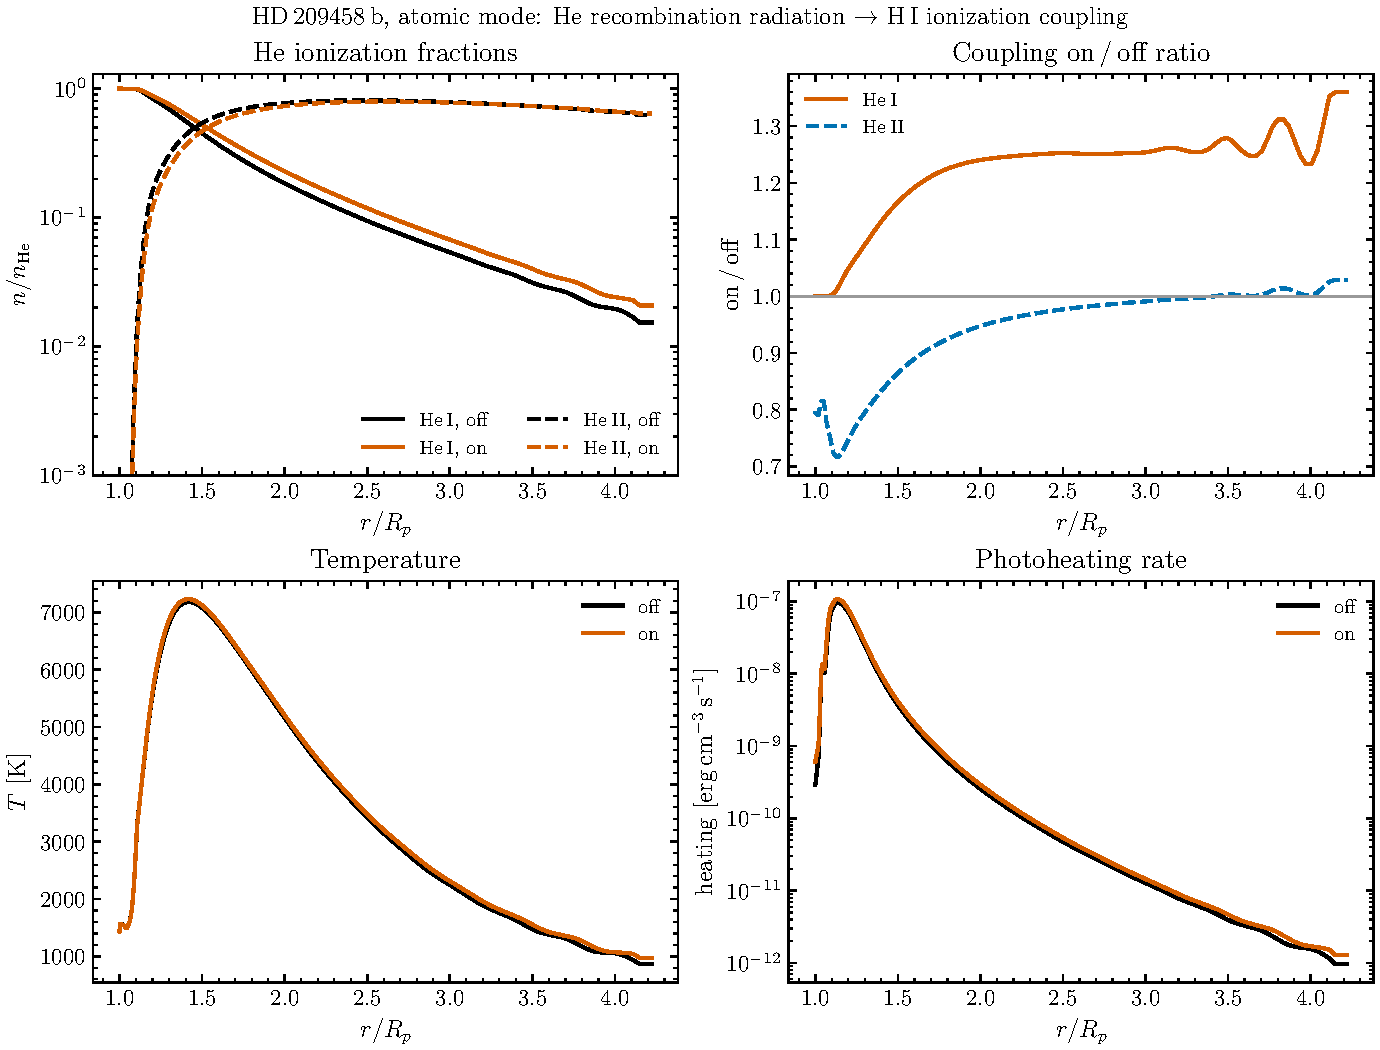
\includegraphics[width=0.98\textwidth]{figures/he_rec_coupling_atomic.pdf}
\caption{He recombination radiation $\to$ H\,I coupling, \textbf{atomic mode}
(HD\,209458\,b). Clockwise from top left: He ionization fractions off vs.\ on;
the on/off ratio for He\,I and He\,II; the photoheating rate; and the
temperature. Turning the coupling on raises He\,I and lowers the He\,II minimum,
with the ${\sim}17\%$ mass-loss increase reflected in the extra photoheating.}
\label{fig:hrc-atomic}
\end{figure}

\begin{figure}[htbp]
\centering
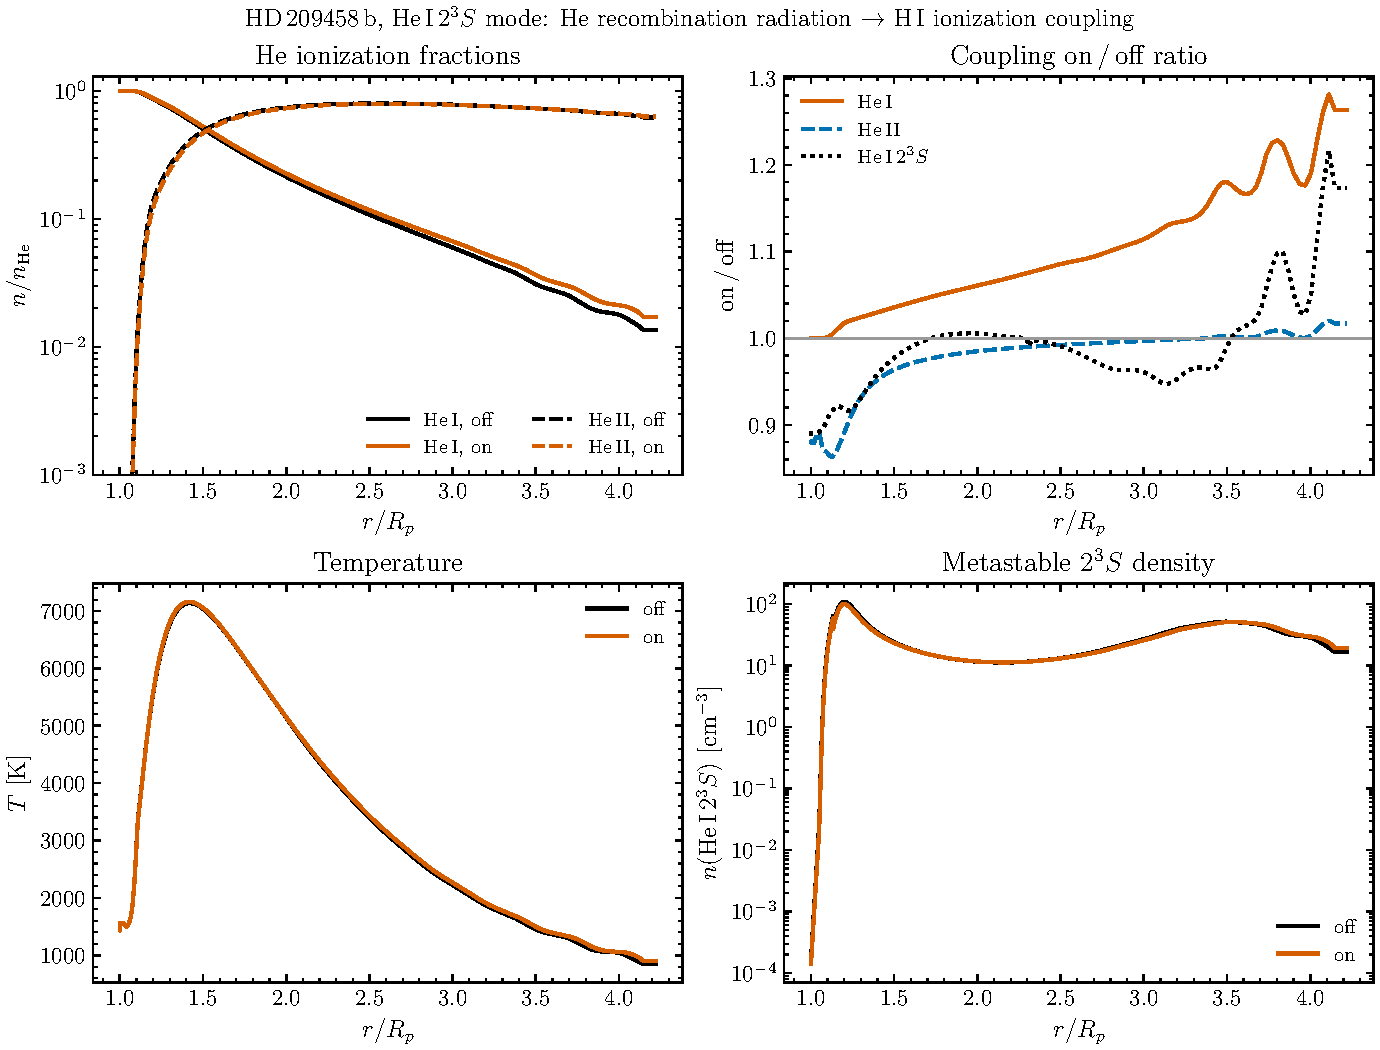
\includegraphics[width=0.98\textwidth]{figures/he_rec_coupling_heitr.pdf}
\caption{Same comparison in the \textbf{He\,I $2^3$S mode}. The extra panel and
ratio curve track the metastable $2^3$S density: it drops ${\sim}11\%$ at the
base but stays within ${\sim}1$--$2\%$ of the off case through the
10830-forming region (1.5--2\,$R_p$), so the He\,I 10830 line is essentially
unchanged.}
\label{fig:hrc-heitr}
\end{figure}

\section{Staged activation of secondary ionization (2026-07-23)}\label{sec:secstage}

\subsection{The regression}
With secondary ionization on by default (the \texttt{use\_sec\_ion} item of the
2026-07-17 rate update), the high-gravity WASP-121\,b cases
(\texttt{backup/regression/wasp\_full}, \texttt{wasp\_he23off}) crashed with a
NaN at ${\sim}$step~587: negative densities first, then a NaN base pressure and
temperature. The coupling itself is physically correct in magnitude --- at the
shielded base the SvS85 secondary channel raises the H photoionization rate by
${\sim}35\times$ over the direct rate, the expected size for the ${\sim}$keV
photoelectrons there. The failure is a transient-path problem, not a
steady-state one: the extra base ionization deepens the base cooling valley and
amplifies the base acoustic mode of the marginal cold initial condition until
the hydro diverges. Two facts pin this down: (a) a run with the coupling off
converges cleanly ($du<10^{-3}$, $\log_{10}\dot M=13.30$); and (b) restarting
with the coupling on from that converged state is benign --- no NaN, $du$ stays
$\lesssim4\times10^{-2}$ during a ${\sim}$2000-step adjustment and re-converges.
The steady state with the full physics exists and is stable; only the cold-start
path to it is fatal.

\subsection{The fix: converge first without the coupling, then switch it on}
A runtime state flag \texttt{sec\_ion\_active} now controls whether the SvS85
partition is applied, separately from the \texttt{use\_sec\_ion} enable flag.
The photoionization / photoheating routines apply the coupling only when
\texttt{use\_sec\_ion .and. sec\_ion\_active}; when it is off the code path is
bit-identical to the \texttt{use\_sec\_ion = False} (full-thermalization) path.
The main loop keeps \texttt{sec\_ion\_active = False} while the wind first
relaxes; the moment that first relaxation reaches a convergence/stall criterion,
the flag flips to \texttt{True}, the convergence logicals and the mass-flux
level-stability history are reset, and the run continues and re-converges with
the full physics. Stops are additionally held for \texttt{N\_stall} (default
2000) steps after the flip: $du$ reacts only once the base adjustment wave driven
by the new coupling has formed, so without the hold the run stopped one step
after activation (activation at step 7144, spurious stop at 7145) with a state
that had not yet incorporated the physics. The Newton (\texttt{Solver: Newton})
finish and the direct-solve diagnostic modes (which bypass the marching loop)
switch the coupling on before their solve, and the flag is forced on after the
loop so post-processing and final outputs always carry the physics even if the
loop hit the iteration cap before the flip.

\subsection{The \texttt{Immediate} override}
\texttt{Secondary\_ionization: Immediate} sets \texttt{use\_sec\_ion = True} and
applies the coupling from step~0, restoring the pre-staging behavior. It is
intended for A/B tests only; on the high-gravity cold-start cases it reproduces
the ${\sim}$step-587 NaN crash, confirming that the staged path is what removes
it.

\subsection{Files touched}
\texttt{parameters.f90} (\texttt{sec\_ion\_active}, \texttt{sec\_ion\_immediate});
\texttt{util\_ion\_eq.f90} (\texttt{PH\_heat\_H} / \texttt{PH\_heat\_HHe} gate on
the local \texttt{sec\_on = use\_sec\_ion .and. sec\_ion\_active});
\texttt{EXHALE\_main.f90} (init, stage flip on first convergence, Newton-finish
and diagnostic-mode activation, post-loop force-on); \texttt{input\_read.f90}
(the \texttt{Immediate} value parsed).

\subsection{Effect on existing results (wasp\_full validation)}
For \texttt{Secondary\_ionization: False} the run is bit-identical to before
(verified byte-identical on \texttt{wasp\_full} and \texttt{wasp\_he23off}). For
the default (staged on) \texttt{wasp\_full}: activation at step 7144,
re-convergence at step 13489 ($du=9.98\times10^{-4}$), and $\log_{10}\dot M$
moves $13.30\to13.22$. The ${\sim}{-}17\%$ mass-loss rate is the real
secondary-ionization physics: the SvS85 partition diverts most of the hard-photon
photoelectron energy from heat into ionization and excitation in the weakly
ionized base, so less energy drives the wind. \texttt{Immediate} reproduces the
old (crashing) behavior on the high-gravity cases.

\section{He-triplet physics series from the Falorca \& Vidotto (2026) review (2026-07-23)}

The line-by-line comparison against Falorca \& Vidotto (2026,
arXiv:2607.18193) and Garc\'ia Mu\~noz (2025, A\&A 698, A199) --- full analysis
in \texttt{docs/falorca2026\_he3d\_review.md} --- exposed six physics gaps, all
implemented and validated in this series (its validation work also surfaced the
secondary-ionization NaN regression fixed in the previous section). Physical
correctness is the acceptance criterion throughout; the impact sizes below are
informational.

\begin{enumerate}
\item \textbf{Penning ionization products}
  (\texttt{heh\_tr\_rows}, \texttt{System\_HeH\_mol},
  \texttt{adv\_implicit\_HeH\_TR}): He($2^3$S)$+$H$^0\to$He($1^1$S)$+$H$^+ + e^-$
  now produces the H$^+$ (with its 6.2\,eV of electron heating,
  $e_{\rm th,HeI}-e_{\rm th,HeTR}-e_{\rm th,HI}$) it always removed the triplet
  for. In the EUV-shielded base ($\Gamma_{\rm HI}$ exponentially small) this is
  the \emph{dominant} H-ionization channel: $n_{\rm HII}$ rises $2$--$7\times$
  at $r<1.03$ on \texttt{wasp\_full}, while the wind and $\dot M$ are unchanged.
  The associative branch ($\to$HeH$^+$, ${\sim}10\%$, GM25) is folded in as
  H$^+$ (documented at the code site).
\item \textbf{Collisional ionization in the TR systems} (\texttt{heh\_tr\_rows}
  $b$ terms; \texttt{ci\_HeI23S} in \texttt{Cool\_coeff.f90}, the
  Black-1981-derived $6.41\times10^{-21}\sqrt{T}\,e^{-55338/T}/E_{23S}$,
  $k(10^4\,\mathrm{K})=3.3\times10^{-10}$): the TR (Oklopcic-form) rows silently
  dropped \emph{all} electron-impact ionization while \texttt{eval\_cool} kept
  charging its cooling --- both restored and consistent now, including CI of the
  metastable itself (a ${\sim}1$--$2\%$ $2^3$S loss at $10^4$\,K, its 4.8\,eV
  cooling in the \texttt{coio} channel, and its He\,I / adv-row counterparts).
\item \textbf{Explicit-$n(2^3S)$ cooling} (\texttt{eval\_cool} $+$ the
  semi-implicit energy solver): the 10830\,\AA{} collisional-excitation channel
  $1.16\times10^{-20}\sqrt{T}\,e^{-13179/T}\,n_e n_{23S}$ (Black form with the
  \emph{explicit} metastable density --- Falorca \& Vidotto warn Black's
  implicit steady-state triplet is wrong here) plus the 0.80/1.40\,eV
  $q_{31a}/q_{31b}$ conversion ledger. The $q_{13}$ (19.8\,eV) term is
  deliberately excluded: the Cen-1992 He\,I excitation-cooling term already
  carries that channel. The terms are passed into
  \texttt{solve\_energy\_semi\_implicit} (all three \texttt{eval\_cool} calls)
  so they act on $T$; without that wiring they were diagnostic-only. Measured:
  $1$--$5\%$ of the total cooling on WASP-121\,b ($8$--$11\%$ of local
  Ly$\alpha$ at the $2^3$S peak), locally up to ${\sim}28\%$ on HD\,209458\,b.
\item \textbf{\texttt{He\_rec\_coupling} default ON} (the previous section has
  the model): with the coupling off the TR singlet recombination used
  $\alpha_1$ alone --- neither case A nor case B --- and the He recombination
  photons ionized/heated nothing. Validated stable on \texttt{wasp\_full}: base
  $n_{2^3S}$ $-10\%$, the 10830-forming region within ${\sim}2\%$, $\dot M$
  unchanged; on HD\,209458\,b $\dot M$ rises $+0.04$--$0.07$\,dex.
  \texttt{He\_rec\_coupling: False} restores the legacy path (byte-identical).
\item \textbf{He$\leftrightarrow$H charge exchange in the default set}
  (\texttt{he\_h\_charge\_exchange}, default on; Koskinen 2013 rates via Huang
  2023 Table~4): the group-B pair moved out of the \texttt{cx\_full}-gated table
  assembly into dedicated \texttt{he\_h\_cx\_fvec/jac/fvec\_adv} routines called
  by \emph{every} ionization system with He (previously only the metals systems
  could reach it), including the advection pair and the analytic Jacobians of
  the Newton systems. The effect is confined to the neutral-H base --- He\,II
  $\times0.59$ at $r=1.05$, $-1\%$ by $r\ge1.2$, $\dot M$ unchanged --- exactly
  the He$^+ +$H$^0\to$He$^0 +$H$^+$ sink where $n_{\rm H^0}$ dominates.
  \texttt{cx\_full} still gates groups C/D. The new input keys of this and the
  preceding sections were also added to the parser's known-keys list (they
  parsed correctly but tripped the unknown-line warning).
\item \textbf{He($2^3$S)$+$H$_2$ Penning ionization}
  (\texttt{penning\_HeI23S\_H2}; \texttt{System\_HeH\_mol} rows 4/5/8 $+$
  4.4\,eV heating): GM25 Table~A.5 (Cohen \& Lane 1977) fitted as
  $5.3791\times10^{-12}\,T^{0.676}\,e^{-695.21/T}$ ($\le0.13\%$ over
  $500$--$10^4$\,K). On the pinned molecular gates the metastable drops
  $39\times$ (HD\,209 base) and $430\times$ (hot-Uranus, out to $r\sim1.1$)
  exactly where $x_{\rm H_2}\to1$, with the upper wind and $\dot M$ unchanged
  --- GM25's dominant deep metastable sink, now present for Tier-2 $+$ triplet
  runs. The \texttt{\_adv} post-process is atomic-only (documented) and needs no
  counterpart.
\end{enumerate}

Regression state after the series: \texttt{Secondary\_ionization: False} $+$
\texttt{He\_rec\_coupling: False} $+$ \texttt{He\_H\_charge\_exchange: False}
reproduce the respective legacy paths byte-identically; the wasp goldens and the
parse-dump corpus were re-snapshotted once at the end of the series (defaults:
staged secondary ionization, He recombination coupling on, He$\leftrightarrow$H
charge exchange on). Converged \texttt{wasp\_full} reference: activation at step
${\sim}7144$, final count ${\sim}13486$, $\log_{10}\dot M=13.22$.

% ===================================================================== %
\section{\texttt{du} triggers require a descending crossing (2026-08-11)}

The \texttt{du} $<$ \texttt{du\_th} convergence stop and the JFNK hand-off (with
the secondary-ionization flip that shares its \texttt{du} test) now fire only
after \texttt{du} has been seen at or above their own threshold. They start armed
for a \texttt{Load IC? True} run and unarmed for a generated IC. The failure this
removes: a transonic IC reported $du(1)=1.85\times10^{-5}$ on WASP-121\,b, which
tripped both triggers on step~1 and ran away to a NaN by step~1220; with the guard
the same input converges (step 8706, $\log_{10}\dot M = 13.21$). The
PLM\,$\to$\,WENO3 switch is deliberately \emph{not} guarded, because the
regression cases legitimately switch on step~1 at $du(1)=0.37$. No new input keys.
Details: \texttt{docs/newton\_scaling\_and\_base\_wall.md} \S9.

% ===================================================================== %
\section{JFNK line search decides on the true residual (2026-08-11)}

The line search in \texttt{solve\_steady\_jfnk} accepted steps on the residual
with the WENO3 smoothness weights frozen at the \emph{previous} iterate, compared
that against a merit memory which mixed the frozen measure with the true one and
was refreshed only on acceptance, and reported both $\lVert R\rVert$ and the
\texttt{info = 0} verdict from the frozen residual. Measured on the HD\,189733\,b
hand-off state: 7 of 14 accepted steps \emph{raised} the true residual, by factors
$1.09$ to $9.05$, and the stored reference stood $2.4\times$ below the true merit
of the iterate the search started from --- which is what produced the
12-consecutive-failure abort.

Trials are now evaluated with the weights recomputed at the trial state, the merit
memory holds true merits and is rewritten at the start of every outer iteration,
and the diagonal scaling is formed before the merit it scales. The frozen weights
still define the inner Newton model, which is where they belong. WASP-121\,b now
reaches \texttt{info = 0} ($\lVert R\rVert = 5.72\times10^{-5}$,
$\log_{10}\dot M = 13.17$, superseding the \texttt{du}-stop $13.21$ of the
preceding section); \texttt{photo\_deep\_secion\_cont} converges in 24 outer
iterations instead of 59; no case exhausts its backtracks any more. No new input
keys, no golden changed. Details:
\texttt{docs/newton\_scaling\_and\_base\_wall.md} \S10.

% ===================================================================== %
\section{Metal-line cooling at a cold base: line trapping and the coronal-fit validity floor (2026-08-11)}

Two physically wrong statements in the metal cooling were corrected. Both bite
only where the gas is cold and dense --- at the base of a planet whose base falls
out of the coronal regime --- and the wind is unaffected.

\subsection{(a) The escape probability was hardwired to 1}
\texttt{eval\_cool} built a \texttt{beta\_esc} from the lowest XUV-band
\emph{continuum} opacity across \emph{one cell}, then overwrote it with
\texttt{beta\_esc = 1.0d0} and applied the full optically thin metal-line cooling
everywhere. Neither quantity is a line optical depth and neither is
grid-independent. (AIOLOS \texttt{chemistry.cpp:1006} instead scales the same gray
depth by an arbitrary $10^{8}$, driving $\beta\to0$ and switching metal-line
cooling off; EXHALE had replaced that with the opposite limit.) Measured on the
converged HD\,189733\,b base, the dominant coolant line
[O\,\textsc{i}]\,63\,$\mu$m carries a line-center optical depth $\tau = 2.7$
through the cold layer, i.e.\ an escape probability of $0.16$, not $1$.

$\beta$ is now the line-center escape probability of the line itself, computed
from the \emph{column} between the emitting cell and the top of the domain
(\texttt{Cool\_coeff.f90}: \texttt{kappa\_OI63}, \texttt{kappa\_CII158},
\texttt{line\_escape\_probability}, \texttt{fine\_structure\_escape}). The shape is
the plane-parallel Doppler result of Hollenbach \& McKee (1979) / de Jong, Boland
\& Dalgarno (1980), renormalized by a factor 2 so that $\beta(0) = 1$
\emph{exactly}: the published form tends to $1/2$ because it counts escape through
one face of a slab, whereas here the other direction is absorbed by the lower
atmosphere and so removes energy from the modeled gas either way. The two branches
are switched at $\tau_c = \sqrt{\pi}\,e^{a^2/4} = 6.967$, where they cross, so the
switch is continuous in value. In the optically thin wind $\beta\to1$, reproducing
the previous behavior.

$\beta$ enters as $A_{ul} \to \beta A_{ul}$ \emph{inside} the two-level solution,
not as a factor on its result: in the subcritical limit the cooling is set by the
collisional excitation rate and must be independent of $\beta$, and multiplying
outside would be wrong by a factor $\beta$ there. Trapping is applied to
[O\,\textsc{i}]\,63\,$\mu$m and [C\,\textsc{ii}]\,158\,$\mu$m only, the two lines
for which the code carries an explicit two-level solution; everything else stays
optically thin, which is right in the wind and is the residual approximation at the
base ($<0.3\%$ of the base cooling there). A thick resonance line in a metal-rich
wind (Mg\,\textsc{ii} h\&k) is still treated as thin --- recorded, not fixed.

\subsection{(b) The CHIANTI coronal fits were evaluated far below their validity floor}
Every metal cooling coefficient in \texttt{Cool\_coeff.f90} is a fit or a table
built over $10^3$--$10^5$\,K. At the 236\,K HD\,189733\,b base, 99.7\% of the
[O\,\textsc{i}] rate came from the fit's softest exponential,
$e^{-930.111/T}$, whose 930\,K corresponds to no [O\,\textsc{i}] ground-term
splitting at all (the splittings are 227.7\,K and 326.6\,K); C\,\textsc{i} is the
same case ($e^{-2351.38/T}$ against splittings of 23.6\,K and 62.4\,K). Below the
floor the only excitable metal transitions are the ground-term fine-structure
lines, which the explicit two-level terms already carry, saturation included.

\texttt{coronal\_excitation\_cutoff(T)} now removes the coronal part below
$10^3$\,K as $\exp[-((T_{\rm floor}/T - 1)/w)^2]$ with $w = 0.5$, and is exactly 1
above it. Value and $dT$-slope are continuous at the floor (the Brent energy solve
and the semi-implicit update both differentiate the cooling in $T$), and every
coefficient is \textbf{bit-identical at and above $10^3$\,K}. The factor is applied
to all CHIANTI-derived coefficients --- the analytic C/N/O and Mg/Ca/Na/Fe forms
and the 1-D/2-D tables, whose $\log_{10}T$ axis starts exactly at 3.0 and which
otherwise hold their edge value indefinitely below it --- and to the coronal
remainder of \texttt{cool\_OI\_ne\_func} / \texttt{cool\_CII\_ne\_func}, but
\emph{not} to their two-level parts. The legacy AIOLOS branch
(\texttt{cno\_cool 0}) is deliberately left alone: its constant floors are crude
fine-structure stand-ins, not extrapolated coronal fits. $w = 0.5$ is a modeling
choice, not a measurement.

\subsection{Measured}
HD\,189733\,b, cell~1: total cooling $3.40\times10^{-5} \to 2.68\times10^{-8}$ erg
cm$^{-3}$ s$^{-1}$ against a heating of $7.0\times10^{-6}$, so the base net rate
changes sign from $-2.65\times10^{-5}$ (cooling) to $+6.97\times10^{-6}$ (heating).
Almost all of that comes from (b); (a) alone is a factor ${\sim}5$ on the
[O\,\textsc{i}] two-level term. Sweeping the code's own cooling assembly in $T$ at
that cell's frozen densities, against the heating measured there, the local
radiative balance temperature moves from \textbf{168\,K to 486\,K} --- 168.2\,K
from (a) alone, 485.5\,K from (b) alone, so (b) does essentially all of the work at
the base --- and the two cooling curves are identical from $10^3$\,K up. A
side-by-side marching test does \emph{not} resolve this: on a $5\times10^4$-step
scale the base is riding an inflow transient whose adiabatic heating dominates the
radiative term in both binaries.

WASP-121\,b (base at 2358\,K, $\tau$([O\,\textsc{i}]\,63\,$\mu$m) $= 0.039$,
$\beta = 0.956$) is unchanged: $\log_{10}\dot M = 13.17$ before and after, outer
mass flux to $3\times10^{-7}$ relative, profile maximum relative difference
$8\times10^{-5}$. \texttt{make check}: \texttt{mol\_base\_handoff} (metals off)
stays byte-identical (PASS); the two metal cases move by the intended physics with
$\log_{10}\dot M = 13.22$ unchanged in both --- \texttt{wasp\_full} maximum
relative difference $3.7\times10^{-7}$ (density), outer mass flux to
$2\times10^{-8}$; \texttt{wasp\_he23off} $1.6\times10^{-3}$ (density, temperature)
in the narrow band at $r = 1.012$--$1.014$, outer mass flux to $1.2\times10^{-5}$.
Goldens not re-snapshotted at that point. Separately noted while comparing: both
goldens already contain \textbf{negative species densities} in that band
(H\,\textsc{i}, O\,\textsc{i}, O\,\textsc{ii}, S\,\textsc{ii}; 17 cells in
\texttt{wasp\_full}, 3 in \texttt{wasp\_he23off}) --- a pre-existing defect,
unrelated to this change.

\subsection{Not fixed by this}
The model still has no stellar optical/IR absorption and no thermal background, so
nothing sets a radiative floor at $T_{\rm eq}$ for a shielded layer; and below
${\sim}700$\,K the guard leaves ions without an explicit two-level term
(C\,\textsc{i}, N, Mg, Ca, Na, Fe) with no cooling at all --- for C\,\textsc{i} that
omits the real [C\,\textsc{i}]\,609/370\,$\mu$m lines, whose LTE rate at the
HD\,189733\,b base is ${\sim}10^{-10}$ erg cm$^{-3}$ s$^{-1}$, i.e.\ $10^{-4}$ of
the local heating. Details: \texttt{docs/hd189\_base\_checkerboard.md} \S10.
Files:
\begin{verbatim}
src/modules/radiation/Cool_coeff.f90
src/modules/radiation/util_ion_eq.f90
src/modules/nonlinear_system_solver/T_equation.f90
src/modules/post_process/post_process_adv.f90
\end{verbatim}

% ===================================================================== %
\section{Base grid resolution as an input key (\texttt{Base grid [dr,cells]}, 2026-08-11)}

The resolution of the uniform region of the \texttt{Mixed} grid was two hardcoded
locals in \texttt{define\_grid.f90} (\texttt{N\_low = 50} cells of
\texttt{drc = 2.0e-4} $R_{\rm p}$). It is now an input key, because that spacing is
what decides whether the base carries the stationary $2\Delta r$ entropy mode
diagnosed in \texttt{docs/hd189\_base\_checkerboard.md}: the controlling parameter
is the number of cells per base density scale height, $H/\Delta r$ with
$H = kT/(\mu g)$, and a $4\times$ refinement was measured to remove the mode.

\begin{verbatim}
Base grid [dr,cells]:  2.0e-4 50     # the default -- the historical grid
Base grid [dr,cells]:  5.0e-5 200    # 4x refinement at the same 0.01 R_p extent
\end{verbatim}

The two numbers share one line, as \texttt{du\_th [PLM,WENO3]} does, because they
are not independent: their product is the radial extent of the uniform region
($0.01\,R_{\rm p}$ by default). Refining at fixed extent means dividing $\Delta r$
and multiplying the cell count by the same factor; changing only one moves the
junction with the stretched region. The second value may be omitted (the count then
keeps its default). The key applies to \texttt{Grid type: Mixed} only;
\texttt{Uniform} and \texttt{Stretched} build their grids from $r_{\max}$ and $N$
alone, and \texttt{EXHALE\_setup.out} echoes that the key is ignored for them.

\texttt{EXHALE\_setup.out} also reports the resolution actually achieved,
\texttt{Base scale-height resolution: H(T\_eq)/dr = 1/(b0*dr\_j(1))} ($b_0$ is the
surface Jeans parameter, \texttt{dr\_j(1)} the first cell after the Mixed-grid
smoothing), and warns below 10 cells. On the default grid this is 26.9 cells for
HD\,189733\,b against 102.3 for WASP-121\,b --- the margin the high-gravity planet
does not have. \texttt{Grid type: Stretched} gives 1.7 cells for HD\,189733\,b,
i.e.\ it is unusable at the base for this class of problem. The smoothing pass at
the end of \texttt{define\_grid} started at the literal \texttt{50}, which was
\texttt{N\_low} written out; it now follows \texttt{N\_low} so that the junction
between the uniform and stretched regions is smoothed wherever it is.

\paragraph{Two costs, both structural.} The CFL step is set by the smallest cell,
so a $4\times$ finer base needs about $4\times$ more steps for the same physical
time. And the total cell count $N = 500$ is a compile-time parameter, so the cells
given to the base come out of the stretched region: on the $4.43\,R_{\rm p}$
HD\,189733\,b domain the stretch ratio goes $1.0119 \to 1.0252$ and the cell size at
$1.5\,R_{\rm p}$ grows from $6.1\times10^{-3}$ to $1.3\times10^{-2}\,R_{\rm p}$.
Refining the base therefore coarsens the wind, which is where $\dot M$ and the
transmission spectrum are formed. Making $N$ runtime-settable would need the static
\texttt{(1-Ng:N+Ng)} arrays to become allocatable throughout; it was not done here.
Recorded while doing this: \texttt{count\_max = 1000000} is also a compile-time
parameter and the \texttt{EXHALE\_MAXSTEPS} hook only lowers it, so a $4\times$
refined base can reach at most $1/4$ of the physical time the default grid reaches
within the cap. On HD\,189733\,b $4\times$ is therefore not reachable to convergence
without raising \texttt{count\_max}; $2\times$ is, and $2\times$ is already where
the mode goes.

\paragraph{Default is bit-exact.} \texttt{dr\_base} is declared with a
\emph{default-real} literal (\texttt{2.0e-4}, not \texttt{2.0d-4}) because that is
what the old local was: the stored value is the single-precision neighbor of
$2\times10^{-4}$, $2.5\times10^{-8}$ relative below it. Declaring the exact double
moves every base cell by that amount; measured on \texttt{wasp\_full} it changed the
converged density by $5\times10^{-10}$ relative (step count and
$\log_{10}\dot M = 13.22$ unchanged), which is not a physics difference but is not
byte-identity either. The literal is kept so that an \texttt{input.inp} without the
key reproduces earlier runs exactly. The consequence to know: writing the default
out explicitly (\texttt{Base grid [dr,cells]: 2.0e-4 50}) does \emph{not} reproduce
it, because the list-directed read into \texttt{real*8} gives the exact double.

\paragraph{Checks.} Byte-identity was tested differentially, against the binary
built immediately before this change rather than against
\texttt{backup/regression/golden/} (the goldens are stale by the intended
metal-cooling physics change of the preceding section). All output files of
\texttt{wasp\_full}, \texttt{wasp\_he23off} and \texttt{mol\_base\_handoff} are
byte-identical including headers, with the same step counts (13488 / 13482 / 12000)
and $\log_{10}\dot M$ (13.22 / 13.22 / 10.58). WASP-121\,b run to completion with
the key absent: $\log_{10}\dot M = 13.17$, JFNK \texttt{info = 0},
$\lVert R\rVert = 5.7\times10^{-5}$ --- unchanged from the preceding section.
Malformed values are rejected in \texttt{define\_grid} (a cell count outside
$[2, N-10]$, or a uniform region that does not fit inside $r_{\max}$).

Details: \texttt{docs/hd189\_base\_checkerboard.md} \S11. Files:
\begin{verbatim}
src/modules/init/parameters.f90
src/modules/init/define_grid.f90
src/modules/files_IO/input_read.f90
src/modules/files_IO/write_setup_report.f90
\end{verbatim}

% ===================================================================== %
\section{Base ghost temperature, runtime step cap, coronal-cutoff width as input keys (2026-08-11)}

Three settings that were compile-time constants or an unexamined default became
\texttt{input.inp} keys. All three default to the previous behavior, so a file without
them runs exactly as before (\texttt{make check}: all three golden cases byte-identical).

\subsection{\texttt{Base ghost temperature: isothermal | continuous}}
The lower ghost cells pin the density to \texttt{rho\_bc} and, in the legacy closure, the
pressure to \texttt{ntot\_bc + dp\_bc}, i.e.\ the temperature to $T_0$. \textbf{The $T_0$
pin has no physical backing}: the radiative equilibrium of the lower atmosphere is outside
the model, so nothing in the code determines the ghost temperature, and $T_{\rm eq}$ is a
choice rather than a boundary condition. It becomes actively wrong once the first interior
cell settles far from $T_0$. With the metal-line cooling of the preceding section, cell~1
on HD\,189733\,b sits at 494\,K against $T_0 = 1183$\,K: a factor-2.4 contact
discontinuity, plus a $2.3\times$ density inversion, held permanently on the boundary.

\texttt{continuous} imposes $dT/dr = 0$ at the base face instead. The ghost keeps the base
composition --- \texttt{ntot\_bc} nuclei and \texttt{dp\_bc} electrons at \texttt{rho\_bc},
exactly the particle count the isothermal pin uses --- and carries the cell-1 temperature,
\begin{equation*}
p_{\rm gh} = (\texttt{ntot\_bc} + \texttt{dp\_bc})\,T_1 ,\qquad
T_1 = p_1 / (n_{\rm tot} + n_e)_1 .
\end{equation*}
$(n_{\rm tot}+n_e)_1$ comes from \texttt{get\_species\_densities}, the single point where
the code decides what counts as a particle. The ghost pressure therefore stays a
differentiable function of the interior pressure (what the JFNK line search needs), while
the ionization state it divides by is lagged exactly like every other composition quantity
across a hydro step. \texttt{BC\_component\_constrho} is the only place the lower ghost is
built, and marching, the JFNK residual and the reconstruction boundary all go through it,
so the closure cannot differ between code paths.

The key sets the same quantity as \texttt{Hydrostatic base: True} (the ghost pressure,
which that key extrapolates from the interior gradient instead), so the two are mutually
exclusive: \texttt{Hydrostatic base} is tested first and \texttt{input\_read} warns when
both appear. With \texttt{Base BC: pressure} the microbar target is imposed at $T_0$ when
$n_0$ is derived, so under a continuous-$T$ ghost only the base \emph{density} stays
anchored; \texttt{input\_read} notes that too. The closure in effect is echoed in
\texttt{EXHALE\_setup.out}.

\paragraph{Measured} on HD\,189733\,b in the production configuration, restarted from the
converged production state and Newton-finished in a scratch copy. The baseline restart
reproduces the stored state digit for digit, so the comparison is like for like.

\begin{center}
\begin{tabular}{lcc}
\toprule
 & \texttt{isothermal} & \texttt{continuous} \\
\midrule
$T_{\rm ghost}$ / $T_1$ [K]            & 1183.0 / 493.6 & 539.9 / 540.2 \\
$\rho_1/\rho_{\rm gh}$                 & 2.33 & 0.95 \\
$A(\ln\rho)$ cells 1--12               & 0.0264 & 0.0092 \\
$A(\ln\rho)$ cells 3--12 / 5--14       & 4.41e-3 / 1.62e-3 & 9.28e-3 / 8.95e-4 \\
JFNK                                   & \texttt{info}\,=\,0, $\lVert R\rVert$\,=\,5.37e-4
                                       & \texttt{info}\,=\,0, $\lVert R\rVert$\,=\,2.76e-4 \\
$\log_{10}\dot M$                      & 9.04 & 9.05 \\
\bottomrule
\end{tabular}
\end{center}

The boundary jump and the density inversion are gone; the extended alternating tail is gone
as well (beyond cell 7 the amplitude drops $13\times$ to $420\times$), and what remains is a
stronger disturbance confined to cells 2--4. Three further restart$+$Newton cycles reproduce
each state digit for digit, so both are exact fixed points and no further decay is available
from cycling. Details, window sweep and scope: \texttt{docs/hd189\_base\_checkerboard.md}
\S13. \textbf{Not} measured at that point: a cold start under the new closure (6\,h,
$10^{6}$ steps), other planets, transit observables.

\paragraph{Adopted for production.} \texttt{HD189733b/input.inp} now carries
\texttt{Base ghost temperature: continuous}, and the planet folder was re-converged with it
together with the ionization-root validation of the next section
(\texttt{run\_20260811\_rootfix.log}): $\log_{10}\dot M = 9.05$, JFNK \texttt{info = 0},
$\lVert R\rVert = 1.72\times10^{-4}$, 2002 steps. Measured on that converged state,
$T_{\rm ghost}/T_1 = 529.4/529.6$\,K, $\rho_1/\rho_{\rm gh} = 0.95$, and $A(\ln\rho)$ over
cells 1--12 is $1.9\times10^{-3}$, i.e.\ well below the 0.0092 of the isolated A/B above ---
the root validation appears to remove a further part of the base disturbance. The paper and
\texttt{python/paper\_data.py} carry 9.05 for this planet.

\subsection{\texttt{Max steps: <N>}}
\texttt{count\_max} was an \texttt{integer, parameter = 1000000}. The preceding section
recorded the consequence: a $4\times$-refined base, whose CFL step is $4\times$ smaller,
cannot reach a converged state within a cap that the default grid already used in full, and
the \texttt{EXHALE\_MAXSTEPS} hook only lowers the cap. \texttt{count\_max} is now a runtime
variable with the same default. \texttt{EXHALE\_MAXSTEPS} keeps its separate meaning (a
deterministic mid-loop exit used by the regression harness); it does not raise
\texttt{count\_max}.

\subsection{\texttt{Coronal cutoff width: <w>}}
The coronal-excitation guard of the preceding section multiplies every CHIANTI-derived
coronal coefficient by $\exp(-x^2)$ with $x = (T_{\rm floor}/T - 1)/w$ below
$T_{\rm floor} = 10^3$\,K. $w = 0.5$ was a hardwired \texttt{parameter}. It is a modeling
choice, not a measured quantity, and the temperature the base settles at depends on it at
the ${\sim}100$\,K level, so it is now settable, still defaulting to 0.5 (division by a
variable holding \texttt{0.5d0} is the same arithmetic, hence byte-identical). Values
$\leq 0$ are rejected at parse time. The manual states the sensitivity where the guard is
documented.

\paragraph{Checks.} \texttt{make check}: \texttt{wasp\_full}, \texttt{wasp\_he23off},
\texttt{mol\_base\_handoff} all byte-identical with the keys absent. WASP-121\,b run to
completion with the keys absent: $\log_{10}\dot M = 13.17$, JFNK \texttt{info = 0},
$\lVert R\rVert = 5.686\times10^{-5}$, 8228 steps, and its output byte-identical to the
same case run with a binary built from \texttt{HEAD} without these changes. The parse-dump
corpus (\texttt{backup/regression/run\_parse\_corpus.sh}) gains three lines per case and
needs a deliberate \texttt{golden} refresh; it was not refreshed there. Files:
\begin{verbatim}
src/modules/init/parameters.f90
src/modules/states/Apply_BC.f90
src/modules/functions/composition.f90
src/modules/radiation/Cool_coeff.f90
src/modules/files_IO/input_read.f90
src/modules/files_IO/write_setup_report.f90
\end{verbatim}

% ===================================================================== %
\section{Ionization-equilibrium roots validated against the physical simplex (2026-08-11)}

\texttt{Ion\_species.txt} carried negative number densities (H\,\textsc{ii},
O\,\textsc{ii}, O\,\textsc{iii}, Fe\,\textsc{i}) in a thin band just above the base: 17
cells at $r = 1.0106$--$1.0140\,R_{\rm p}$ in the \texttt{wasp\_full} golden, 15 cells in
the WASP-121\,b production run, 5 in HD\,189733\,b.

The equilibrium systems are polynomial in the stage fractions and possess roots outside the
physical simplex. At the step where secondary ionization is switched on (step 7186 of
\texttt{wasp\_full}) MINPACK \texttt{hybrd1} returned \texttt{info = 1} on such a root ---
$x$(H\,\textsc{ii}) $= -5.2\times10^{-6}$, the Fe stage fractions summing to 1.2209, i.e.\ an
Fe\,\textsc{i} density 22\% below zero. Nothing tested the root, and the next step's warm
start re-seeded the solve from the same values, so the state reproduced itself for the
remaining 6302 steps. The heating paid for it twice: the metal photoheating channel went
negative ($-6.6\times10^{-7}$ erg cm$^{-3}$ s$^{-1}$, which is impossible), and the ionized
fraction, clamped into $[0,1]$, sent the Spitzer \& Scott (1985) heating fraction
$f_{\rm heat}$ to zero, switching off every photoheating channel above the photoelectron
threshold. Total heating in the band sat 93\% below its neighbors. Clamping the offending
fractions to zero is therefore not a repair --- the clamp is exactly what produces
$f_{\rm heat} = 0$; the cure has to be a physical root, not a clipped one.

Every atomic cell solve now validates its root --- each stage fraction $\geq 0$, and each
element's ionized stages summing to at most its nucleus total --- and on failure restarts
from physically defined starting points: the uncoupled ionization balance at the incoming
electron density (\texttt{ionization\_balance\_at\_fixed\_ne}, admissible by construction,
since the stage populations of a three-stage element come out proportional to
$(d_1d_2,\,u_0d_2,\,u_0u_1)$), then the optically thick fully neutral limit. A stored state
that is not physical no longer seeds the next solve, which is what breaks the
self-sticking. A cell where no starting point produces an admissible root is left on the
ionization balance and reported rather than accepted. A first attempt that converges to a
physical root is accepted unchanged, so healthy cells follow exactly the same solver path
as before. \texttt{q\_abs}, an absorbed energy rate, must now be positive before it
normalizes the heating efficiency.

\paragraph{Gates} (single-threaded; a baseline \texttt{make check} on the same tree passed
all three cases, so the differences are this change alone). \texttt{wasp\_full} FAILs by
intent: negative densities 17 cells $\to$ 0, $\log_{10}\dot M$ 13.22 $\to$ 13.22,
$T/\rho/v/p$ within 0.89\%/0.77\%/1.3\%/0.13\% of the golden away from the band, metal
photoheating positive everywhere (domain minimum $-8.9\times10^{-7} \to +1.03\times10^{-7}$).
\texttt{wasp\_he23off} also FAILs: its golden looks clean but the run reports 35 roots
outside the simplex over 13478 steps, previously accepted in silence; $\dot M$ unchanged,
$T/\rho/p$ within 0.28\%/0.086\%/0.039\%. \texttt{mol\_base\_handoff} is byte-identical.
The two production runs, each re-run once with the pre-change binary and once with the fix
so the comparison isolates this change, keep their mass-loss rates and step counts
(WASP-121\,b 13.17, 8228 steps; HD\,189733\,b 9.05, 2002 steps) and lose their negative
densities entirely. HD\,189733\,b is the clearest demonstration of the self-sticking: its
stored initial condition is one of the poisoned outputs, and at step~1 the run rejects
exactly the 5 stored cell states that carried negative densities and resolves all of them.
Goldens were not re-snapshotted at that point.

\paragraph{Not covered.} The molecular network keeps its own chemical-equilibrium retry and
is left alone; the H-only system (no helium) and the post-processing advection solves in
\texttt{post\_process\_adv.f90} are outside this validation, and the advected profiles of
HD\,209458\,b still carry small negative H\,\textsc{ii}, He\,\textsc{iii} and He\,$2^3S$
entries in the first 14 cells above the base. Full account:
\texttt{docs/ionization\_root\_validation.md}. Files:
\begin{verbatim}
src/modules/radiation/ionization_equilibrium.f90
src/modules/radiation/util_ion_eq.f90
src/modules/nonlinear_system_solver/newton_solver.f90
src/EXHALE_main.f90
\end{verbatim}

% ===================================================================== %
\section{Line trapping in the thick metal resonance lines: measured, no change (2026-08-11)}

The metal-cooling section above introduced $\beta(\tau)$ for
[O\,\textsc{i}]\,63\,$\mu$m and [C\,\textsc{ii}]\,158\,$\mu$m and recorded the thick
resonance lines of a metal-rich wind (Mg\,\textsc{ii} h\&k, Ca\,\textsc{ii} H\&K,
Na\,\textsc{i} D, the Fe\,\textsc{ii} UV multiplets) as an untreated case. They were
measured on the converged WASP-121\,b, HD\,209458\,b and HD\,189733\,b runs.
\textbf{No code path changed.}

The lines are thick --- Mg\,\textsc{ii} k reaches $\tau_0 = 7.6\times10^{4}$ at the
WASP-121\,b base and stays above $10^{2}$ through the region where Mg\,\textsc{ii} carries a
third of the local cooling, and over 99\% of the integrated Mg\,\textsc{ii} /
Ca\,\textsc{ii} / Fe\,\textsc{ii} / Mg\,\textsc{i} cooling comes from gas with
$\tau_0 > 1$. That is not the test, though. Trapping lengthens the random walk of a
resonance photon; it does not destroy it. In two-level equilibrium the correction to an
optically thin coronal fit is
\begin{equation*}
S = \frac{\beta A_{ul}}{\beta A_{ul} + n_e q_{ul}} ,\qquad
q_{ul} = 8.629\times10^{-6}\,\Upsilon/(g_u\sqrt{T}) ,
\end{equation*}
not a factor $\beta$, so it bites only above
$n_{\rm crit,eff} = \beta A_{ul}/q_{ul}$. For these permitted lines
$A_{ul}\sim10^{8}$\,s$^{-1}$, so even at $\beta\sim10^{-6}$ the escape rate keeps
$n_{\rm crit,eff}$ at $10^{9}$--$10^{15}$\,cm$^{-3}$, against a maximum $n_e$ of
$4.3\times10^{9}$\,cm$^{-3}$ in the WASP-121\,b run. The forbidden fine-structure lines are
the opposite case ($A_{ul}\sim10^{-5}$--$10^{-3}$\,s$^{-1}$,
$n_{\rm crit,eff}\sim10^{0}$--$10^{5}$\,cm$^{-3}$), which is why they, and only they, need
$\beta$.

Measured $\Delta\Lambda$ integrated over the wind: \textbf{0.0214\%} of the total radiative
losses of WASP-121\,b, 0.0022\% of HD\,209458\,b, 0.0015\% of HD\,189733\,b. The largest
local effect is 1.65\% in the first WASP-121\,b cell, whose $T$ is pinned at $T_{\rm eq}$ by
the boundary condition; the loss exceeds 0.1\% only below $r = 1.007\,R_{\rm p}$. Per line
it is 0.1\% of the Mg\,\textsc{ii} cooling, 0.015\% of Ca\,\textsc{ii}, 1.4\% of
Na\,\textsc{i} (its $A_{ul}$ is the smallest of the set) and 0.02--0.8\% of
Fe\,\textsc{ii}. The measurement is a conservative bound: it uses the Doppler-core escape
probability, which understates $\beta$ by $4$--$10\times$ for these Voigt profiles, and no
turbulent broadening.

Checked in passing: the Fe\,\textsc{ii} $a^6D$ fine-structure lines at
25.99/35.35\,$\mu$m, the one metal transition with an $A_{ul}$ small enough to trap, reach
only $\tau_0 \leq 0.06$, so the \texttt{cool\_FeII\_ne} statistical-equilibrium table needs
no escape probability either. H\,\textsc{i} Ly$\alpha$, outside this scope, has
$\tau_0 = 1.3\times10^{8}$ and a cooling-weighted $S = 0.9994$ --- two-level trapping is
therefore not what suppresses Ly$\alpha$ cooling, and the destruction channels that could
(photoionization of H($n=2$), collisional $2p \to 2s$) were not evaluated.

$\beta = 1$ for the resonance lines is kept and is now documented at the code site as a
justified effective treatment with its validity condition, in the \texttt{SCOPE} comment of
\texttt{src/modules/radiation/Cool\_coeff.f90}, instead of an acknowledged omission. Full
measurement: \texttt{docs/resonance\_line\_trapping.md}.

% ===================================================================== %
\section{Metal electrons and a validity range for the post-process advection correction (2026-08-12)}

Two defects in \texttt{post\_process\_adv}, both confined to the
advection-corrected \texttt{*\_adv.txt} output: the post-processor is the last call of the
run and its arguments are \texttt{intent(in)}, so the converged wind and the equilibrium
\texttt{*.txt} files cannot be affected by anything here.

\paragraph{The electron density inside the advection residuals was wrong.} It counted only
the H and He electrons, while the equilibrium residual it corrects counts the metal
electrons as well (\texttt{metal\_electron\_sum}) and the \emph{same} routine already used
the metal-inclusive $n_e$ for its heating, cooling and temperature solve. In a shielded base
the metals are the dominant electron donors --- measured
$n_{e,\rm metal}/n_e = 0.48$--$1.00$ in the base cells of all four paper planets --- so the
recombination terms were low by up to six orders of magnitude. Solved
to machine precision with Brent, the residual \emph{as coded} had its fixed point at
$x_{\rm H\,II} = 4.74\times10^{-8}$ in the first HD\,209458\,b cell, against an equilibrium
$7.46\times10^{-14}$. A field \texttt{adv\_cell\%xe\_metal} now carries the metal electrons
per H nucleus into all three advection residuals, with the definition \texttt{calc\_ne} and
\texttt{metal\_electron\_sum} use. It is not conditioned on \texttt{eos\_include\_metals}:
that switch decides whether the metals enter the mass and particle budget, whereas
recombination needs the true electron density. Metals off gives zero identically.

\paragraph{The correction was applied where it cannot be computed and is not needed.} The
residuals carry the \emph{neutral} fraction and report the ion density as
$(1-x_{\rm H\,I})\,n_h$, so the ion fraction inherits the solver's absolute resolution on
$x_{\rm H\,I}$, $\mathrm{xtol} = \sqrt{\epsilon} = 1.5\times10^{-8}$. Where the equilibrium
ion fraction is $10^{-13}$ the returned value is quantized at $10^{-8}$ with an arbitrary
sign: the first HD\,209458\,b cell got $x_{\rm H\,II} = -4.96\times10^{-8}$ where the exact
root is $+4.74\times10^{-8}$ --- right magnitude, wrong sign --- and the upwind cascade
carried the negative density outward over 14 cells. Those same cells are in local ionization
equilibrium to
\begin{equation*}
{\rm Da} = \frac{\Delta r}{v}\,\left(\Gamma_{\rm H\,I} + \alpha_{\rm H\,II} n_e\right)
         = 350\text{--}2900 ,
\end{equation*}
so the equilibrium solution is the answer the ODE would give anyway. The correction is now
skipped, and the converged equilibrium ionization kept, wherever the cell is (i) inflowing
($v \leq 0$ on either face: the upwind discretization has no upstream cell), (ii)
equilibrium-dominated (${\rm Da} > 100$) or (iii) unrepresentable
($x_{\rm H\,II,eq} < 10^{-6}$, less than 1\% relative accuracy at that resolution).
Conditions (i) and (ii) are statements about the flow and (iii) about the representation of
the unknown, so the pre-existing \texttt{pp\_metal\_on} gate on the inflow condition is
removed --- it made a property of the discretization depend on the metal-cooling switch. The
temperature loop keeps condition (i) alone, likewise ungated; a thermal Damk\"ohler number
is not evaluated. Clipping the extracted densities at zero was tested and rejected: it
breaks the H nucleus budget $n_{\rm H\,I} + n_{\rm H\,II} = n_h$.

\paragraph{Gates.} \texttt{make check}: PASS, all three cases byte-identical (the goldens
compare \texttt{Hydro\_ioniz.txt} and \texttt{Ion\_species.txt}, which this does not write).
Isolated A/B, the pristine \texttt{HEAD} binary and the modified one run from the same
configuration: \texttt{Hydro\_ioniz.txt}, \texttt{Ion\_species.txt},
\texttt{Cooling\_breakdown.txt} and \texttt{Excited\_H.txt} byte-identical, only the
\texttt{\_adv} files differ.

\begin{center}
\small
\begin{tabular}{lccccc}
\hline
planet & $\dot M$ [log g/s] & negative \texttt{\_adv} & cells held at eq (newly) & outermost held & max change, $r>1.05$ \\
\hline
HD\,209458\,b & $9.31 \to 9.31$   & $48 \to 0$ & $103 \to 124$ (21) & $1.0316$ & 1.4\% (He\,\textsc{iii}) \\
HD\,189733\,b & $9.05 \to 9.05$   & $0 \to 0$  & $135 \to 212$ (77) & $1.0380$ & 0.37\% (He\,\textsc{iii}) \\
WASP-121\,b   & $13.17 \to 13.17$ & $0 \to 0$  & $0 \to 0$ (0)      & ---      & 3.8\% (He\,\textsc{iii}) \\
WASP-52\,b    & $11.63 \to 11.63$ & $0 \to 0$  & $3 \to 57$ (54)    & $1.0106$ & 3.3\% (He\,\textsc{iii}) \\
\hline
\end{tabular}
\end{center}

Every cell whose equilibrium ion fraction is below $10^{-6}$ is now held at the equilibrium
value, and no newly held cell lies above $r = 1.038\,R_{\rm p}$. The change in the wind is
entirely the metal electrons: a build carrying the guard alone removes all 48 HD\,209458\,b
negative entries by itself and changes the profiles above $r = 1.05\,R_{\rm p}$ by exactly
zero on three of the four planets and by $4.2\times10^{-5}$ on WASP-52\,b. Transmission spectra move by at most 0.07\% in peak depth (He\,10830 of
HD\,209458\,b) and 0.08\% in equivalent width (H$\alpha$ of WASP-121\,b).

The re-run reproduces the stored \texttt{output/} of WASP-121\,b and WASP-52\,b
byte-identically but not that of HD\,209458\,b and HD\,189733\,b, which restart from
\texttt{output/*\_IC.txt} files that had been refreshed to the previous run's converged
state; re-running continues that convergence (HD\,209458\,b $du$:
$1.199\times10^{-2} \to 3.13\times10^{-3}$) and moves the profiles by up to 9\% in density
at unchanged $\dot M$. That is unrelated to this change --- the pristine binary follows the
same new trajectory --- and is why the table above is an A/B between two binaries.

Files:
\begin{itemize}\itemsep0pt\parskip0pt
\item \texttt{src/modules/post\_process/post\_process\_adv.f90}
\item \texttt{src/modules/nonlinear\_system\_solver/ion\_cell\_state.f90}
\item \texttt{src/modules/nonlinear\_system\_solver/System\_implicit\_adv\_\{H,HeH,HeH\_TR\}.f90}
\end{itemize}
Full account: \texttt{docs/postprocess\_advection\_validity.md}.

Found and \textbf{not} fixed, marked at the code site: \texttt{System\_implicit\_adv\_HeH}
(helium on, He\,$2^3$S off) writes its electron-impact ionization terms without the
$n_e n_h$ factor that \texttt{adv\_implicit\_H}, \texttt{adv\_implicit\_HeH\_TR} and the
equilibrium rows all carry, which also makes them dimensionally inconsistent with the
photoionization rates they are added to. None of the four paper planets uses that path.
(Since fixed, 2026-08-12: the terms now carry \texttt{ionhi*xe*n\_h}; commit
\texttt{b0d44bc}, TO\_BE\_DONE item~(B).)

% ===================================================================== %
\section{Ground-term fine-structure statistical equilibrium for C\,I, C\,II, N\,II and O\,I (2026-08-12)}

The CHIANTI C/N/O cooling fits carry the ground-term fine-structure (FS) lines in the
optically thin, \emph{low-density} limit. Their critical densities are of order
$10^{0}$--$10^{5}\,\mathrm{cm^{-3}}$, decades below the base density of an irradiated
atmosphere ($n_e\sim10^{9}$, $n_{\rm H\,I}\sim10^{14}\,\mathrm{cm^{-3}}$), so at the base
the coronal form overstates what those lines can radiate by 2.9--8.3 decades. Two of them
([O\,\textsc{i}] 63\,$\mu$m, [C\,\textsc{ii}] 158\,$\mu$m) already had a two-level
saturation; C\,\textsc{i}, N\,\textsc{ii} and the [O\,\textsc{i}] 145.5/44\,$\mu$m channels
did not, and C\,\textsc{i} was in consequence the dominant coolant of the whole base layer
of HD\,189733\,b, at a value comparable to the local heating rate.

\paragraph{What replaces it.} Every C/N/O coolant whose ground term is split now has that
term solved in exact statistical equilibrium at the local $(n_e, n_{\rm H\,I})$,
\begin{equation*}
\sum_j f_j R_{ji} = f_i \sum_j R_{ij},\qquad \sum_i f_i = 1,
\end{equation*}
\begin{equation*}
R_{ul} = C_{ul} + \beta_{ul}A_{ul},\qquad
R_{lu} = C_{ul}\,\frac{g_u}{g_l}\,e^{-E_{ul}/k_BT},\qquad
C_{ul} = n_e k_{e,ul}(T) + n_{\rm H\,I}\,k_{{\rm H},ul}(T),
\end{equation*}
\begin{equation*}
W_{\rm FS} = \sum_{u>l} f_u\,\beta_{ul}A_{ul}\,k_B E_{ul}
\qquad [\mathrm{erg\,s^{-1}}\ \mathrm{per\ ion}],
\end{equation*}
and the coronal curve is refitted to keep only the channels that \emph{leave} the ground
term ($\Lambda_{\rm rem}$). The coefficient handed to the assembly is
$\Lambda_{\rm eff} = W_{\rm FS}/n_e + \Lambda_{\rm rem}$, so the $n_e n_{\rm ion}$ prefactor
recovers the H-collision channel exactly. Treated: C\,\textsc{i} $2p^2\,^3P$
(609.1/370.4\,$\mu$m), C\,\textsc{ii} $2p\,^2P$ (157.7\,$\mu$m), N\,\textsc{ii} $2p^2\,^3P$
(205.3/121.8\,$\mu$m), O\,\textsc{i} $2p^4\,^3P$ (63.2/145.5/44.1\,$\mu$m). That is the
complete set --- N\,\textsc{i} and O\,\textsc{ii} have a single-level $^4S$ ground term,
Mg\,\textsc{i}/\textsc{ii}, Ca\,\textsc{ii} and Na\,\textsc{i} a single ground level,
Fe\,\textsc{i} is built from permitted lines only, and Fe\,\textsc{ii} already uses a
two-dimensional statistical-equilibrium table.

Limits: $n_e, n_{\rm H\,I}\to0$ collapses onto the ground level and reproduces the coronal
within-term channel to the accuracy of the collision-strength fits (1.3--4.4\%); high
density saturates at the exact multilevel LTE emission (verified to $10^{-14}$ relative).
$\beta_{ul}$ enters inside the solution, not as a factor on the result, which is the only
placement that is right in both limits. All eight lines with a transition probability now
get their own line-center escape probability from the outward column; previously only two
did.

\paragraph{Two defects fixed on the way.} (i) The two-level form multiplied a solution
already normalized to the two-level partition function by the ground-term Boltzmann
fraction of its lower level, so its LTE limit was low by $1+(g_u/g_l)e^{-E/k_BT}$ ---
$2.7\times$ for [C\,\textsc{ii}] 158\,$\mu$m at the 530\,K base of HD\,189733\,b. (ii) The
H-atom de-excitation rates (a constant $4.0\times10^{-11}$ for C\,\textsc{ii},
$4.2\times10^{-11}(T/100)^{0.67}$ for O\,\textsc{i}, both flagged approximate in the source)
are replaced by fits to published quantum scattering calculations: Yan \& Babb (2023,
MNRAS 518, 6004) for C\,\textsc{i} and N\,\textsc{ii}, Abrahamsson, Krems \& Dalgarno
(2007, ApJ 654, 1171) for O\,\textsc{i}, Barinovs et al.\ (2005, ApJ 620, 537) for
C\,\textsc{ii}. They are 5--20$\times$ larger.

\paragraph{What it does.} The \texttt{coronal\_excitation\_cutoff} guard was standing in for
the missing saturation, so its width $w$ behaved as a tuning knob on the base temperature.
It no longer does: the local balance temperature of the base cell is identical to every
digit printed over $w = 0.02$--$1.2$ on all four planet runs, against a 500--650\,K spread
before.

\begin{center}
\small
\begin{tabular}{lcc}
\hline
run & base $T$ & $\dot M$ at $2\,R_{\rm p}$ \\
\hline
HD\,189733\,b (warm restart, $w = 0.1$) & $528.5 \to 613.2$\,K & $2.351\times10^{9} \to 2.850\times10^{9}$ g/s ($+21.2\%$) \\
WASP-121\,b (cold start)                & $2406.9 \to 2438.8$\,K & $3.106\times10^{13} \to 3.370\times10^{13}$ g/s ($+8.5\%$) \\
\texttt{wasp\_full} golden case         & $2340.6 \to 2357.3$\,K & $3.482\times10^{13} \to 3.549\times10^{13}$ g/s ($+2.0\%$) \\
\hline
\end{tabular}
\end{center}

Transit depths on HD\,189733\,b move by $+4.4\%$ (Ca\,\textsc{ii}) to $+20.7\%$
(H$\beta$). The profiles outside $r \sim 1.1\,R_{\rm p}$ move by a few percent; the change
is a base-layer change that propagates through the density.

Files:
\begin{itemize}\itemsep0pt\parskip0pt
\item \texttt{src/modules/radiation/Cool\_coeff.f90} --- the SE solvers, the four ion
  coefficients, the generalized line opacity and escape routine
\item \texttt{src/modules/radiation/util\_ion\_eq.f90}
\item \texttt{src/modules/nonlinear\_system\_solver/T\_equation.f90}
\item \texttt{src/modules/post\_process/post\_process\_adv.f90}
\item \texttt{cooling\_data/fit\_fs\_saturation.py} --- generator; prints every coefficient
\item \texttt{cooling\_data/make\_cooling\_doc\_figures.py}
\item \texttt{docs/cooling\_formulas.tex}, \texttt{docs/coronal\_cutoff\_width.md}
  section 7, \texttt{TO\_BE\_DONE.md} item (C)
\end{itemize}

Also fixed here, unrelated but found while reading the cooling diagnostics:
\texttt{examples/exhale\_io.py} named only four fixed channels in
\texttt{Cooling\_breakdown.txt} while the writer emits six (the collisional-excitation
channel is written split by absorber), so every metal column was labeled two ions too early.
\texttt{python/paper\_data.py} parses the header and was already correct.

Still open: with the artifact gone it is plain that the base is not in local radiative
balance at all --- at the HD\,189733\,b base the total radiative cooling is
$3.5\times10^{-8}$ against a heating of $3.4\times10^{-6}$. Its temperature is set by the
inner boundary and by the flow.

% ===================================================================== %
\section{Base ghost built from the composition of the state it bounds (2026-08-12)}

\texttt{Apply\_BC} closes the \texttt{Base ghost temperature: continuous} ghost with
\begin{equation*}
p_{\rm ghost} = (\texttt{ntot\_bc} + \texttt{dp\_bc})\,
                \frac{p(1)}{\texttt{n\_part\_cell1}} ,
\end{equation*}
where \texttt{n\_part\_cell1} is the cell-1 particle count written by
\texttt{get\_species\_densities}. Two call sites filled the ghosts before any composition
solve had run on the state in question, so they used whatever \texttt{n\_part\_cell1} was
left over --- the \texttt{input\_read} placeholder $\texttt{ntot\_bc} + \texttt{dp\_bc}$ in
the first case:

\begin{itemize}\itemsep0pt\parskip0pt
\item \texttt{init.f90}: the initial \texttt{Apply\_BC}. On HD\,189733\,b the placeholder
  differs from the true cell-1 particle count by 4.4\%, and the finite-volume steady
  residual of the loaded state (which stops right after \texttt{init}) reported the
  resulting contact discontinuity at the base face as a cells 1--2 spike of 60 (mass) and
  120 (energy) per sound crossing time.
\item \texttt{steady\_newton.f90}, \texttt{eval\_residual}: \texttt{Apply\_BC} after
  \texttt{unpack\_U}. There $F(Y)$ depended on the previous $Y$ as well as on $Y$, so a
  finite-difference Jacobian column mixed two states.
\end{itemize}

Both now evaluate the composition of the interior first. \texttt{init.f90} also seeds
\texttt{base\_flux\_const} from the initial state, for the same reason: with
\texttt{Base velocity: massflux} that constant starts at $-1$, which \texttt{Apply\_BC}
reads as ``not available yet'' before falling back to the valve, so the first step and any
diagnostic stopping right after \texttt{init} used a different velocity boundary condition
than the run. Files: \texttt{src/modules/init/init.f90},
\texttt{src/modules/time\_step/steady\_newton.f90}.

\paragraph{Checks.} \texttt{n\_part\_cell1} is read only by the continuous branch and
\texttt{base\_flux\_const} only by the mass-flux branch, so a run setting neither key is
unaffected and \texttt{make check} is byte-identical; an \texttt{isothermal} HD\,189733\,b
residual reproduces bit for bit. With the key on, the cells 1--2 mass residual falls from
$5.97\times10^{1}, 5.92\times10^{1}$ to $6.41\times10^{-2}, 7.70\times10^{-2}$ and the
energy residual from $1.12\times10^{2}, 1.20\times10^{2}$ to $1.31\times10^{-1},
1.54\times10^{-1}$, with cell 3 outward and the wind window unchanged to every digit.
Re-converging the planet from its stored state: JFNK scaled merit $\lVert F_s\rVert_2$
$1.43 \to 0.315$, \texttt{info = 0}, $\log_{10}\dot M$ $9.15 \to 9.14$. Measurements and
term-by-term split: \texttt{docs/hd189\_base\_checkerboard.md} section 15.

% ===================================================================== %
\section{H($n=2$) rate coefficients, the trapped-$2p$ balance, and de-excitation heating (2026-08-12)}

Four corrections to the excited-hydrogen and Ly$\alpha$ modules, plus the structural change
that made the first one possible. Measurement and the full number tables:
\texttt{docs/lya\_destruction\_channels.md} section 11.

\paragraph{One definition of the $n=2$ rate coefficients.} The Ly$\alpha$ and $n=2$ atomic
data and every collisional rate coefficient existed in three copies --- inside
\texttt{n2\_populations}, again as standalone functions in the same file, and a third time
in \texttt{lya\_rt.f90}. They are now one module,
\texttt{src/modules/radiation/hydrogen\_n2\_rates.f90}, which exports
\texttt{c1s2s\_rate}, \texttt{c1s2p\_rate}, \texttt{c2s2p\_rate}, \texttt{c2s1s\_rate},
\texttt{c2p1s\_rate}, \texttt{c2p2s\_rate}, \texttt{alpha\_B\_hydrogen},
\texttt{alpha\_2s\_hydrogen}, \texttt{alpha\_2p\_hydrogen},
\texttt{n2p\_destruction\_rate} and the line constants.
\texttt{excited\_hydrogen.f90} and \texttt{lya\_rt.f90} use it.

\begin{enumerate}\itemsep2pt\parskip0pt
\item \textbf{Statistical weights shadowed by dummy arguments.} \texttt{n2\_populations} was
  declared \texttt{(T, n1s, ne\_l, Jlya, G2s, G2p, n2s, n2p)}. Fortran does not distinguish
  \texttt{G2s} from the module parameter \texttt{g2s}, so the three detailed-balance rate
  coefficients written out in the routine body evaluated their weights as the Balmer
  photoionization rate the caller passed: $2s\to1s$ and $2p\to1s$ de-excitation came out 5
  to 306 times too small (planet-dependent, scaling with the stellar Balmer continuum) and
  the $2p\to2s$ $\ell$-mixing rate 3 times too large. The dummies are now
  \texttt{gam\_ion\_2s} / \texttt{gam\_ion\_2p} and the body calls the shared rate
  functions, so the weights are resolved at module scope and out of a dummy's reach. Two
  further shadows of the same kind, both harmless, were renamed: the frequency-sample count
  \texttt{ng = 400} in \texttt{gamma\_n2\_balmer} and \texttt{heat\_n2\_balmer} shadowed the
  global ghost-cell count \texttt{Ng}; it is \texttt{n\_nu}.
\item \textbf{Recombination cascade source.} \texttt{a2s*ne**2} / \texttt{a2p*ne**2}
  $\to$ \texttt{a2s*ne*nHII} / \texttt{a2p*ne*nHII}. The electron recombines onto a proton;
  at the base the electrons come largely from helium and metals while hydrogen is still
  neutral, and $n_e/n_{\rm H\,II}$ reaches 2 on WASP-121\,b and $5\times10^{6}$ on
  HD\,209458\,b. The Python transmission tool (\texttt{exhale\_transit\_lib.py},
  \texttt{EXHALE\_transit.py}) and \texttt{examples/tpm\_halpha\_lart2d.py} carried the same
  expression and were corrected the same way; their \texttt{n2\_populations} signatures
  gained an \texttt{nHII} argument.
\item \textbf{Destruction channels in the \texttt{J\_int} closure.} \texttt{lya\_rt.f90}
  built the trapped field from $n_{2p} = P/(A_{2p\to1s}\beta)$. The $2p$ budget also loses
  atoms to collisional de-excitation, $n=2$ photoionization, and $\ell$-mixing followed by
  two-photon decay; the denominator is now $A_{2p\to1s}\beta + D$ with $D$ from
  \texttt{n2p\_destruction\_rate}. Where $\beta$ is smallest the omission over-estimated
  \texttt{J\_int} by up to $1.5\times$. In the same module the top-down Ly$\alpha$
  line-center optical depth, previously two identical inline loops, is the single routine
  \texttt{lya\_line\_center\_optical\_depth}; all three \texttt{jlya\_mode} values call it,
  so the \texttt{tau\_Lya} column of \texttt{Excited\_H.txt} is filled in the LaRT import
  mode instead of being written as zero.
\item \textbf{\texttt{Deexc heat} now defaults on.} The comment justifying the old
  default --- that collisional de-excitation heating overlaps the H\,\textsc{i}
  collisional-excitation cooling --- was wrong: \texttt{coex\_rate\_HI} is the one-way Cen
  (1992) coronal rate with no de-excitation term in it, so \texttt{Hdx} is the correction to
  that limit, not a double count. Most of the $n=2$ population it de-excites was pumped by
  Ly$\alpha$ rather than excited by a collision, which makes the term absorbed Ly$\alpha$
  thermalized by a collision, the same size as the photoelectric heating the code already
  applied unconditionally. The key now also honors \texttt{Deexc heat: False}, which it
  previously ignored. \textbf{This changes results for any run that supplies a stellar
  $T_{\rm eff}$/radius and does not set the key.}
\end{enumerate}

Audited and left alone: the energy equation applies no escape-probability factor to the
Ly$\alpha$ cooling. \texttt{cool} is built from the bare Cen coefficient
(\texttt{Cool\_coeff.f90:843} $\to$ \texttt{util\_ion\_eq.f90:640,787}); $\beta$ appears
nowhere in that path, in any \texttt{jlya\_mode}. That is the correct form --- 98.2--99.99\%
of trapped Ly$\alpha$ photons escape and the collisional destruction that would suppress the
cooling is at most 0.06\% --- so the historical expectation of a ${\sim}10\times$ transfer
suppression is not in the code and should not be.

\paragraph{Checks.} \texttt{mol\_base\_handoff} (no stellar $T_{\rm eff}$, so the excited-H
model is off) is byte-identical at every stage, as is its comparison against the stored
golden. \texttt{wasp\_full} and \texttt{wasp\_he23off} move: $\log_{10}\dot M$
$13.23039 \to 13.22966$ and $13.23106 \to 13.23026$, with the largest local temperature
change 0.57\% (item 1), 0.081\% (item 2) and 0.147\% (item 3); both cases pin
\texttt{Deexc heat: True} in their \texttt{input.inp}, so item 4 moves nothing in them.
Their goldens were already stale against the pre-fix tree and were left as they are.
Re-converged from their stored initial conditions in a scratch copy, WASP-121\,b gives
$13.2075 \to 13.2030$, HD\,189733\,b $9.1286 \to 9.1392$ and HD\,209458\,b
$9.3790 \to 9.4581$; the H$\alpha$ and H$\beta$ transit depths move by 0.4--1.7\%
($n(2p)$, which carries the opacity, barely moves, while $n(2s)$ halves). HD\,209458\,b is
the largest move (0.075 dex, from items 1--3) because its Ly$\alpha$ cooling is a negligible
share of its radiative losses while the $n=2$ heating terms are not; it is also the case
\texttt{docs/lya\_deexcitation\_heating.md} recorded as going NaN at the base with the
de-excitation heating on, which no longer reproduces with the corrected populations
(re-converges from its stored initial condition, and a cold start survives a 20000-step
cap). A build at \texttt{-O1 -fopenmp -g -fcheck=bounds,do,mem} running the
\texttt{wasp\_full} configuration is clean.

Files:
\begin{itemize}\itemsep0pt\parskip0pt
\item \texttt{src/modules/radiation/hydrogen\_n2\_rates.f90} (new)
\item \texttt{src/modules/radiation/excited\_hydrogen.f90},
  \texttt{src/modules/radiation/lya\_rt.f90}
\item \texttt{src/modules/init/parameters.f90},
  \texttt{src/modules/files\_IO/input\_read.f90}, \texttt{Makefile}
\item \texttt{exhale\_transit\_lib.py}, \texttt{EXHALE\_transit.py},
  \texttt{examples/tpm\_halpha\_lart2d.py}
\end{itemize}

% ===================================================================== %
\section{Molecular chemistry and trace metals solved in one system (2026-08-13)}

The parser refused \texttt{Molecular chemistry: True} together with a \texttt{metals.inp}.
That refusal blocked two things: the deep ($10^{-3}$\,bar) lower-atmosphere handoff of
\texttt{docs/base\_composition\_handoff\_plan.md} \S11.7, whose A/B pair carries metals and
whose consistent configuration is Tier-2 molecular chemistry; and trace-metal work on
sub-Neptunes, which have a molecular base by construction.

The two networks cannot be solved apart, and the reason is quantitative rather than
architectural: \textbf{in the shielded molecular base the metals supply essentially all the
free electrons.} Measured at the base cell of the two smoke tests below, with solar metal
abundances:

\begin{center}\small
\begin{tabular}{lccc}
\hline
case & $n_e$ with metals [cm$^{-3}$] & metal share & $n_e$ metals-off [cm$^{-3}$] \\
\hline
hot Uranus, solar 7 metals & $1.20\times10^{8}$ & $1.000$ & $6.29\times10^{4}$ \\
HD\,209458\,b, $10^{-3}$\,bar handoff, C/N/O & $9.42\times10^{5}$ & $0.990$ & $9.27\times10^{4}$ \\
\hline
\end{tabular}
\end{center}

The flux that ionizes the low-ionization-potential metals --- Mg\,I at 7.65\,eV, Fe\,I at
7.90\,eV, C\,I at 11.26\,eV --- lies below both the H\,I edge (13.60\,eV) and the H$_2$
threshold (15.4\,eV), so it is absorbed by neither and reaches the base almost
unattenuated. On the hot-Uranus case it holds Mg and Fe about 1.6\% ionized at the base,
which is already enough to swamp the H/He and molecular electrons. Every recombination and
electron-impact term of the molecular network scales with $n_e$, so solving the network at
the metal-free $n_e$ misses a factor 1900 (hot Uranus) to 10 (HD\,209458\,b at
$10^{-3}$\,bar) in that layer.

\paragraph{The merged system.} \texttt{System\_HeH\_mol\_metals} follows the pattern
\texttt{System\_HeH\_TR\_metals} established: the molecular unknowns keep their rows, the
metals are appended above them, and both blocks are shared code rather than re-derived. The
eight balance rows of the molecular network moved into \texttt{mol\_heh\_rows} (still in
\texttt{System\_HeH\_mol}, with the Koskinen 2022 rate coefficients, which stay defined in
exactly one module) and take $n_e$ as an input, exactly as \texttt{heh\_tr\_rows} does; the
metal rows, the metal electron sum and the stage fractions come from
\texttt{ion\_residual\_core} unchanged. The layout is
\begin{center}\small
\begin{tabular}{@{}ll@{}}
\texttt{x(1..3)} & H\,II, He\,II, He\,III \\
\texttt{x(4..7)} & H$_2$, H$_2^+$, H$_3^+$, HeH$^+$ \\
\texttt{x(8)}    & He\,$2^3$S (when tracked) \\
\texttt{x(mbase..)} & $X^{+}$, $X^{++}$ for each metal element, \texttt{mbase = metal\_row\_base() = 8 or 9} \\
\end{tabular}
\end{center}
with $N_{\rm eq} = 7$ ($+1$ with the triplet) $+\,2\,n_{\rm melem}$.
\texttt{metal\_row\_base()} is the single definition of that offset, read by the residual,
by the driver's seeding and root validation, and by \texttt{cx\_metal\_base} so that the
Huang Table-4 charge exchange writes to the shifted metal rows. With
\texttt{met\_nelem = 0} the system reduces exactly to \texttt{System\_HeH\_mol}.

\paragraph{Root validation and seeding (\S45 extended to the molecular branch).} The
molecular cell solve is bistable because the cell is: a molecular basin (the dense,
optically thick base) and an atomic basin (the wind above the H$_2\to$H front). It now
tries one starting point in each in turn --- the warm start, the chemical-equilibrium
H$_2$ fraction at the local $(p,T)$ with the metal stages from their own ionization balance
at the incoming $n_e$, then the molecule-free ionization balance of every element --- and
keeps a converged root only if it is also physical, on the same rule \S45 applied to the
atomic systems. The metal part of \texttt{ionization\_balance\_at\_fixed\_ne} was split into
\texttt{metal\_ionization\_balance\_at\_fixed\_ne} so the molecular retry seeds its metals
from the same balance instead of a second copy of it. The third starting point is what the
front cells needed: on the hot-Uranus case the coupled solve leaves 3 cells at
$r = 1.21$--$1.22$ (the ionization front) with no admissible root at every step with two
starting points, and 0 cells with three.

\paragraph{Two defects found in the surrounding code and fixed.}
\begin{itemize}\itemsep2pt\parskip0pt
\item The sub-13.6\,eV energy grid of a power-law spectrum was an \texttt{if
  (thereis\_HeITR) \dots else if (thereis\_lowIP\_metal)}, with the comment that the
  triplet and metals together are unsupported so at most one applies. That has not been true
  since the triplet and the metals were merged. With the triplet on, the grid floor stopped
  at 4.80\,eV, which is above the K\,I threshold (4.341\,eV), so K\,I would be held
  spuriously neutral in a triplet run. The floor is now the lowest threshold over whichever
  sources are active, matching what the loaded-SED path (\texttt{sed\_read}) already did. No
  golden carries K, so this is byte-identical there.
\item The \texttt{pp\_metals 2} metal re-solve passed the global $N_{\rm eq}$ to
  \texttt{hybrd1} while its residual (\texttt{ion\_system\_metals\_pp}) writes only rows
  $1..3+2\,n_{\rm melem}$. With the He\,$2^3$S triplet that already left one row of
  \texttt{fvec} unwritten; with the molecular layout it would leave four or five. It is now
  sized $3 + 2\,n_{\rm melem}$ with a matching workspace, the same reasoning
  \texttt{lwa\_adv} already carried a few lines above. Both goldens run \texttt{pp\_metals
  1}, so this is byte-identical there and changes results only for \texttt{pp\_metals 2}
  runs.
\end{itemize}

\paragraph{Left in place at the time, with the validity range written at the code.}
\texttt{eval\_cool} built its own electron density without the molecular ions. That is right
in the hot atomic gas it was written for and wrong inside a deep molecular base, where
H$_3^+$ can be the dominant ion; there it disagreed with the $n_e$ the equilibrium solver
itself uses (\texttt{ionization\_equilibrium} does pass \texttt{nmol\_eq} to
\texttt{calc\_ne}), so the $n_e$-scaling cooling channels were under-counted in that layer.
Two definitions of the same quantity is one too many, but closing the gap changes the
molecular results and belonged in its own change with its own measurement. \emph{Closed in
the next section.}

\paragraph{Gates.} \texttt{make check} PASSes byte-identical on all three cases then in the
matrix (\texttt{wasp\_full}, \texttt{wasp\_he23off}, \texttt{mol\_base\_handoff}); a
baseline \texttt{make check} on the same tree before the change also passed, so the
comparison is this change alone. Goldens were not re-snapshotted. A build at \texttt{-O1
-fopenmp -g -fcheck=bounds,do,mem} is clean on all three coupled layouts for 200--300 steps:
hot Uranus with the He\,$2^3$S triplet ($N_{\rm eq} = 28$, metals at row 9), the same case
without it ($N_{\rm eq} = 27$, metals at row 8), and the HD\,209458\,b deep handoff.

Hot Uranus (the Tier-2 gate configuration of
\texttt{docs/lower\_atmosphere\_figs/data\_g2}) plus solar C/N/O/Mg/Ca/Na/Fe, a 12000-step
relaxation snapshot against the same case metals-off: the H$_2\to$H front sits at
$r = 1.1577$ in both (the gate's $1.156$), the base stays fully molecular in both,
$\log_{10}\dot M = 10.58$ in both, no negative densities, and no cell is left without an
admissible root (the same case with the triplet off, $N_{\rm eq} = 27$ with the metals at
row 8, is clean over a shorter 400-step smoke). What the metals change is the base
chemistry: $n_e$ rises $1900\times$ and H$_3^+$ falls by a factor 1350
($7.08\times10^{4} \to 52.5$\,cm$^{-3}$), its peak moving out from $r = 1.040$ to
$r = 1.130$ --- H$_3^+$ is destroyed by dissociative recombination (Koskinen R6/R7, both
proportional to $n_e$), so it survives only where the metal electron fraction starts to
fall. Metal ionization runs the expected way: C\,II/C $= 8\times10^{-10}$ at the base, 0.22
at the front, 0.43 at $1.9\,R_{\rm p}$; Mg\,III stays below $10^{-8}$ up to the front and
reaches $2.4\times10^{-3}$ only at $1.9\,R_{\rm p}$.

HD\,209458\,b at the $10^{-3}$\,bar handoff (the \S11.7 blocker), C/N/O, He\,$2^3$S on, a
4000-step bounded run: it integrates. \S11.7 records that the atomic pair built at this
level terminated with a NaN at $r = 1.067$ after 1846 steps with the time step collapsed to
$dtu = 1.2\times10^{-6}$ (that run was not repeated here); this one reaches the cap with
$dtu = 0.198$ and no NaN, a fully molecular base, and the front at $r = 1.0150$ ($1.0169$
metals-off). It is a relaxation snapshot at $du = 747$, nowhere near converged, so no
mass-loss rate should be read off it.

\paragraph{Open item.} The \texttt{\_adv} post-process is still molecule-free by design
(\texttt{post\_process\_adv.f90} header): \texttt{nh = nhi + nhii} counts only the free H
nuclei and the molecular electrons are absent from its $n_e$. The metal stages are carried
there as usual under \texttt{pp\_metals}, but on that molecule-free H/He background, so
\texttt{\_adv} metal profiles inside the molecular layer inherit the approximation. With the
\texttt{eval\_cool} electron density closed in the next section, this is the one remaining
place where a molecular run and a metal run still meet on the atomic assumption.

Files:
\begin{itemize}\itemsep0pt\parskip0pt
\item \texttt{src/modules/nonlinear\_system\_solver/System\_HeH\_mol\_metals.f90} (new)
\item \texttt{src/modules/nonlinear\_system\_solver/System\_HeH\_mol.f90}
\item \texttt{src/modules/radiation/ionization\_equilibrium.f90},
  \texttt{src/modules/radiation/util\_ion\_eq.f90}
\item \texttt{src/modules/files\_IO/input\_read.f90},
  \texttt{src/modules/files\_IO/write\_setup\_report.f90} (the startup report now names the
  species blocks the coupled system carries and prints $N_{\rm eq}$)
\item \texttt{src/modules/init/set\_energy\_vectors.f90},
  \texttt{src/modules/post\_process/post\_process\_adv.f90}, \texttt{Makefile}
\item \texttt{examples/16\_molecular\_metals/} (new)
\end{itemize}
Documentation: \texttt{README.md}, \texttt{README\_HOWTO.md},
\texttt{examples/README.md}, \texttt{docs/EXHALE\_user\_manual.tex} (the example table also
became a \texttt{longtable}, which it needed already --- as a float it ran past the bottom
margin into the page footer), \texttt{docs/input\_schema.md},
\texttt{docs/lower\_atmosphere\_coupling.md},
\texttt{docs/base\_composition\_handoff\_plan.md}.

% ===================================================================== %
\section{One electron density for the cooling and for the ionization solver (2026-08-13)}

\texttt{eval\_cool} rebuilt its own free-electron density and left the molecular ions out of
it. The equilibrium solver in the same sweep does not: it balances ionization against
\texttt{calc\_ne(nhii,nheii,nheiii,ne,nm,nmol\_eq)}, i.e.\ H$^+$, He$^+$, He$^{++}$, the
metal stages under the \texttt{eos\_metals} policy, \textbf{and} H$_2^+$, H$_3^+$, HeH$^+$.
A molecular run therefore carried two definitions of $n_e$, and the cooling used the smaller
one. That is wrong wherever a molecular ion carries a non-negligible share of the charge,
which is exactly the deep molecular base. Measured on the metals-off hot-Uranus Tier-2 gate,
the two definitions differ by $\mathbf{168.5\times}$ at the base cell (373 against
$6.29\times10^{4}\,\mathrm{cm^{-3}}$, H$_3^+$ supplying essentially all of it), $4.5\times$
at $r = 1.05$, 2.8\% at $r = 1.10$, and nothing above $r \sim 1.15$; on the
\texttt{mol\_base\_handoff} case the base ratio is $175.7\times$.

\texttt{eval\_cool} now takes an optional \texttt{nmol} (H$_2$, H$_2^+$, H$_3^+$, HeH$^+$,
cgs) and passes it straight to \texttt{calc\_ne} --- the electron density is not
reconstructed anywhere inside \texttt{eval\_cool}, it has one definition and one
implementation. Callers that track the molecular network supply it:
\texttt{ionization\_equilibrium} (\texttt{nmol\_eq}), the semi-implicit energy solver
(\texttt{nmol\_dim}, the cgs copy of the adimensional array it already hands
\texttt{calc\_ne}/\texttt{calc\_ntot}), and the \texttt{Cooling\_breakdown} dump. The
\texttt{\_adv} advection post-process deliberately does not: that reconstruction is
molecule-free by design (its module header), and omitting the argument gives it the atomic
charge sum it is built on. \texttt{ionization\_equilibrium}'s own \texttt{calc\_ne} call
lost its \texttt{thereis\_mol} branch at the same time --- \texttt{nmol\_eq} is zero for an
atomic run, so one call covers both.

Every $n_e$-scaling channel picks the correction up: recombination, collisional ionization,
collisional excitation and bremsstrahlung are linear in $n_e$, and the coronal metal line
coefficients enter as \texttt{ne*nm*c\_metal}. The saturated ground-term coefficients
(Fe\,II, and C\,I/C\,II/N\,II/O\,I under \texttt{cno\_chianti}) are
$\Lambda_{\rm eff} = W/n_e$, so the assembly's $n_e$ cancels and they respond only through
the level populations ($C_{21}\propto n_e$) --- the correct behavior, and there is no double
counting of $n_e$ anywhere in \texttt{eval\_cool}.

\paragraph{Atomic runs are exactly unchanged.} \texttt{nmol\_eq} and the molecular
\texttt{f\_sp} columns are zero, and \texttt{calc\_ne} adds them as
\texttt{ne + 1.0*0.0}, which is exact. \texttt{make check} is byte-identical on
\texttt{wasp\_full} (metals $+$ He\,$2^3$S) and \texttt{wasp\_he23off}; a full WASP-121\,b
run (metals, He\,$2^3$S, Ly$\alpha$ escape probability, excited H, transonic IC) reproduces
all eight output files byte-identically --- \texttt{Hydro\_ioniz\{,\_adv\}},
\texttt{Ion\_species\{,\_adv\}}, \texttt{Cooling\_breakdown},
\texttt{Heating\_breakdown}, \texttt{Excited\_H}, \texttt{IC\_dump} --- at
$\log_{10}\dot M = 13.20$.

\paragraph{\texttt{mol\_base\_handoff} changes, and that is the point of the change.} At the
pinned 12000-step snapshot the two runs stop at the same $du = 2.6689$ and the same
$dtu$; every hydrodynamic column agrees to $\leq 4\times10^{-8}$ relative and every species
column to $\leq 4.2\times10^{-6}$ (that worst case is H$_3^+$ at $r = 2.96$, where H$_3^+$
is $3\times10^{-19}\,\mathrm{cm^{-3}}$). The one column that moves is the reported cooling
rate at the near-neutral base, $2.799\times10^{-20} \to 4.942\times10^{-18}$
erg\,cm$^{-3}$\,s$^{-1}$ ($\times176.5$, the $n_e$ ratio, as expected for channels linear in
$n_e$). $\log_{10}\dot M$ stays 10.58.

\paragraph{Why the dynamics barely notice.} A molecular layer cools through the H$_3^+$
infrared lines, which do not scale with $n_e$, so multiplying the electron channels by 176
at the base moves the cooling from $2.8\times10^{-20}$ to $4.9\times10^{-18}$ against
$1.3\times10^{-7}$ erg\,cm$^{-3}$\,s$^{-1}$ of photoheating there. The correction is real
and it is now the same quantity the solver balances ionization against, but it is
energetically negligible in the layer where it is large.

\paragraph{Molecular smoke tests.} Hot Uranus, the Tier-2 gate configuration, 12000-step
relaxation snapshots --- both runs stop at $du$ of order unity, so these are snapshots and
not converged solutions.

\begin{center}\small
\begin{tabular}{lcc}
\hline
 & metals off & metals on (solar C/N/O/Mg/Ca/Na/Fe) \\
\hline
$n_e$(base) old $\to$ new & $373 \to 6.29\times10^{4}$\,cm$^{-3}$ ($\times168.5$)
  & $1.2016\times10^{8} \to 1.2016\times10^{8}$ ($\times1.0000$) \\
cooling at the base & $3.18\times10^{-20} \to 5.36\times10^{-18}$ erg/cm$^3$/s
  & $+7\times10^{-7}$ relative \\
H$_2\to$H front & $1.15631 \to 1.15631$ & $1.15677 \to 1.15677$ \\
H$_3^+$ peak & $7.0808\times10^{4} \to 7.0807\times10^{4}$\,cm$^{-3}$ at $r = 1.0396$
  & $52.465 \to 52.465$ at $r = 1.1304$ \\
$du$ at step 12000 & $4.3354 \to 4.2914$ & $5.8177 \to 5.8177$ \\
$\log_{10}\dot M$ & $10.58 \to 10.58$ & $10.58 \to 10.58$ \\
\hline
\end{tabular}
\end{center}

The metals-on column is the expected null: the low-ionization-potential metals hold $n_e$ at
$1.2\times10^{8}$ at that base (previous section), against $52\,\mathrm{cm^{-3}}$ of
H$_3^+$, so adding the molecular ions moves nothing (maximum relative change $7\times10^{-10}$
in $\rho$/$T$/$p$, $3\times10^{-9}$ in the metal stages). Metals-off, the snapshot differs by
1\% in $du$ and by sub-percent in the bulk state just above the layer ($\rho$ $-0.7$\%, $T$
$+0.8$\% at $r = 1.19$), with the trace species that depend exponentially on $T$ amplifying
that into H$_3^+$ $-16$\%, H$_2$ $-13$\%, He\,II $+10$\% at the same radius. Those are
differences between two snapshots of an unconverged relaxation, not a converged shift; the
gate observables --- front position, H$_3^+$ peak, mass-loss rate --- are unchanged.

On the HD\,209458\,b $10^{-3}$\,bar handoff with C/N/O (a 4000-step bounded snapshot, also
unconverged) the base picture is the same: the metals dominate $n_e$, the base cooling rises
0.45\%, the molecular-layer cooling by at most 1.9\%, the front moves
$1.01503 \to 1.01518$ and the H$_3^+$ peak by 0.05\%. An
\texttt{-O1 -fopenmp -g -fcheck=bounds,do,mem} build runs all three molecular layouts (hot
Uranus with and without metals, HD\,209458\,b deep handoff) for 300 steps with no runtime
check firing.

\paragraph{Two related items found and recorded, not changed here.}
\begin{itemize}\itemsep2pt\parskip0pt
\item The H$_3^+$ infrared cooling is added to \texttt{cool} in
  \texttt{ionization\_equilibrium}, \emph{after} \texttt{eval\_cool} returns. The JFNK
  steady residual uses that array, but the semi-implicit energy update (the default)
  rebuilds \texttt{cool} from \texttt{eval\_cool} alone and overwrites it, so it never sees
  the H$_3^+$ term. For a molecular run the marching stage and the Newton stage therefore
  integrate slightly different energy equations, and the marching fixed point is not the
  zero of the residual the Newton solver drives down. The fix is to move the term inside
  \texttt{eval\_cool} (which already receives \texttt{nmol}) with its own \texttt{cool\_chan}
  column; that changes the \texttt{Cooling\_breakdown.txt} schema and the molecular results,
  so it belongs in its own change. The \texttt{Cooling\_breakdown} header now states that
  the channel sum falls short of the \texttt{cool} column by that term in the molecular
  layer. Open item (F) of \texttt{TO\_BE\_DONE.md}.
\item H$_2^+$, H$_3^+$ and HeH$^+$ donate their electron to $n_e$ but are left out of the
  bremsstrahlung charge sum, so that sum is smaller than $n_e$ inside the molecular layer.
  They are $Z_{\rm ion} = 1$ and belong there formally, but they only exist at
  $T \sim 10^{3}$\,K, where the hot-plasma free-free expression is an extrapolation emitting
  at frequencies the atmosphere is not thin to, and where free-free is negligible against
  the H$_3^+$ and metal line cooling. The scope is written at the accumulator.
\end{itemize}

Files:
\begin{itemize}\itemsep0pt\parskip0pt
\item \texttt{src/modules/radiation/util\_ion\_eq.f90},
  \texttt{src/modules/radiation/ionization\_equilibrium.f90}
\item \texttt{src/modules/time\_step/energy\_semi\_implicit.f90}
\item \texttt{src/modules/post\_process/post\_process\_adv.f90} (comments only)
\end{itemize}
Documentation: \texttt{docs/lower\_atmosphere\_coupling.md}.

% ===================================================================== %
\section{A fourth regression case for the molecular $+$ metals system (2026-08-13)}

The coupled molecular $+$ metals system of the section before last was not guarded by
anything in the matrix: \texttt{mol\_base\_handoff} runs the molecular network metals-off,
and the two \texttt{wasp\_*} cases run metals without molecules, so the merged residual, the
\texttt{metal\_row\_base()} offset and the three-starting-point seeding had no golden.

\texttt{backup/regression/mol\_metals} is that case: the same hot-Uranus Tier-2 gate
configuration as \texttt{mol\_base\_handoff} (\texttt{Molecular chemistry: True}, its
\texttt{base.inp} handoff, 12000 steps pinned in \texttt{maxsteps}) plus a solar-abundance
\texttt{metals.inp} with the seven elements C/N/O/Mg/Ca/Na/Fe. It stops at $du = 3.1770$,
$\log_{10}\dot M = 10.58$. \texttt{DEFAULT\_CASES} in
\texttt{backup/regression/run\_check.sh} is now
\texttt{wasp\_full wasp\_he23off mol\_base\_handoff mol\_metals}, and the case list in the
script header describes what each one guards.

Goldens for all four cases were re-snapshotted at the end of this change series, so they
carry the two preceding sections. The two atomic cases are byte-identical to their previous
goldens (both changes are exact no-ops without molecules); \texttt{mol\_base\_handoff} moves
only in its cooling column, by the factor 176.5 of the previous section.

One harness trap, hit while doing this and now written into the script: \texttt{golden} does
\textbf{not} re-run the cases, it copies whatever \texttt{output/} currently sits in each
case directory. Snapshotting straight after a code change baselines the \emph{previous}
binary. The order is \texttt{check} (which rebuilds and re-runs), then \texttt{golden}, then
\texttt{check} again.

Files: \texttt{backup/regression/run\_check.sh},
\texttt{backup/regression/mol\_metals/} (new), \texttt{backup/regression/golden/}
(re-snapshotted). Documentation: the workspace \texttt{CLAUDE.md},
\texttt{README\_HOWTO.md}.

\section{H$_3^+$ infrared cooling inside \texttt{eval\_cool}: one energy equation for a
molecular run (2026-08-13)}

Closes item (F) of \texttt{TO\_BE\_DONE.md}, opened by the audit in the section before last.

The H$_3^+$ infrared cooling was added to \texttt{cool} in \texttt{ionization\_equilibrium},
\emph{after} \texttt{eval\_cool} returned. Only some of the consumers of \texttt{cool} saw it:

\begin{center}\small
\begin{tabular}{>{\raggedright\arraybackslash}p{0.40\textwidth}>{\raggedright\arraybackslash}p{0.20\textwidth}>{\raggedright\arraybackslash}p{0.28\textwidth}}
\hline
term in \texttt{cool} & rebuilt by \texttt{energy\_semi\_implicit} (the default marching
  temperature update) & returned by \texttt{ioniz\_eq} (JFNK steady residual, the
  explicit-energy option, the in-loop $\lVert R\rVert$ monitor, the
  \texttt{Hydro\_ioniz.txt} cool column) \\
\hline
H/He recombination & yes & yes \\
collisional ionization (H\,I, He\,I, He\,II, He\,$2^3$S) & yes & yes \\
collisional excitation (H\,I Ly$\alpha$, He\,I, He\,II, He\,$2^3$S 10830 $+$
  $2^1$S/$2^1$P conversion) & yes & yes \\
bremsstrahlung (H$^+$, He$^+$, He$^{++}$, metal ions) & yes & yes \\
metal line cooling (27 ions, saturated ground-term fine structure included) & yes & yes \\
\textbf{H$_3^+$ infrared (Miller et al.\ 2013)} & \textbf{NO} & \textbf{yes} \\
\hline
\end{tabular}
\end{center}

\texttt{heat} has no such split: it is assembled once in \texttt{ioniz\_eq} (photoheating by
each absorber including H$_2$ and the metals, Shull \& van Steenberg secondary-ionization
partition, Balmer photoelectric and Ly$\alpha$ de-excitation, He-recombination coupling,
He\,$2^3$S $+$ H and He\,$2^3$S $+$ H$_2$ Penning) and passed into
\texttt{energy\_semi\_implicit} as \texttt{intent(in)}, never rebuilt. H$_3^+$ was the only
asymmetric term, and it was the whole asymmetry.

Three consequences followed from that one row.

\begin{itemize}
\item \textbf{The marching fixed point was not the zero of the residual the Newton solver
  drives down.} The marching relaxed $\Gamma = \Lambda_{\rm atomic+metal}$; the residual
  demanded $\Gamma = \Lambda_{\rm atomic+metal} + \Lambda_{\rm H_3^+}$.
\item \textbf{The two energy-solver options integrated different equations.}
  \texttt{Energy solver: Explicit} used the \texttt{ioniz\_eq} array directly and did carry
  the term; the semi-implicit default (the production setting) did not.
\item \textbf{The \texttt{cool} column of \texttt{Hydro\_ioniz.txt} meant different things
  depending on how the run stopped.} A \texttt{du}-stop left the semi-implicit array (no
  H$_3^+$) in place; the JFNK finish calls \texttt{ioniz\_eq} after
  \texttt{solve\_steady\_jfnk} and left the array that has it.
\end{itemize}

\paragraph{Size of the missing term.} On the metals-off hot-Uranus Tier-2 gate
(\texttt{backup/regression/mol\_base\_handoff}) the H$_3^+$ lines carry \textbf{more than
99\% of the total radiative cooling from the base out to the H$_2 \to$ H front}
(\texttt{Cooling\_breakdown} H3p\_IR / cool\_total $> 0.5$ over $r = 0.9998$--1.1856, $>
0.99$ over 0.9998--1.1557), peaking at $9.35\times10^{-7}$\,erg\,cm$^{-3}$\,s$^{-1}$ at
$r = 1.0413$, which is \textbf{7.3$\times$ the local photoheating}. Below the front every
atomic channel is exponentially suppressed at $T \sim 1.3\times10^{3}$\,K, so the marching
stage was integrating that layer with essentially no radiative loss at all: the cooling it
used was smaller than the true total by a factor $1.1\times10^{2}$ to $1.2\times10^{11}$
over $r = 1.00$--1.156. With solar trace metals (\texttt{mol\_metals}) the metal lines
dominate instead and H$_3^+$ reaches only 22\% of the local cooling, in a thin band
$r = 1.066$--1.193.

\paragraph{The fix.} \texttt{eval\_cool} computes the H$_3^+$ cooling itself, from the
\texttt{nmol} array it has taken since the section before last, using the same
\texttt{h3p\_cooling} module (one definition of the Miller et al.\ 2013 fits and the
Table-6 non-LTE factor; \texttt{eval\_cool} \texttt{use}s it, nothing is re-derived). The
post-return addition in \texttt{ionization\_equilibrium} is gone, and a comment at the
\texttt{eval\_cool} call states why nothing may be added there. \texttt{cool\_chan} gains
column 7 for the channel, so the decomposition still reproduces \texttt{cool} exactly
(measured $\max |\sum_{\rm channels}/{\rm cool} - 1| = 3.3\times10^{-16}$ on the molecular
gate, $5.5\times10^{-16}$ on \texttt{wasp\_full}). Callers that model a molecule-free gas
(\texttt{post\_process\_adv}, and \texttt{T\_equation} which solves for the \texttt{\_adv}
temperature) omit \texttt{nmol} and therefore still get the atomic charge sum \emph{and} no
H$_3^+$ term --- the same approximation, stated at both call sites.

A side effect worth naming: \texttt{energy\_semi\_implicit} builds its damping derivative
$\mathrm{d}C/\mathrm{d}T$ by finite-differencing \texttt{eval\_cool} in temperature, so the
steep temperature dependence of the H$_3^+$ emission now enters the implicit temperature
update instead of being invisible to it.

\paragraph{Output schema.} \texttt{Cooling\_breakdown.txt} gains \texttt{col11 H3p\_IR}; the
27 metal-ion columns move from 11--37 to 12--38. It is written for every run and is zero
without the molecular network. \texttt{python/paper\_data.py} reads the column names from
the header and follows automatically; \texttt{examples/exhale\_io.py} has a fixed list,
which now carries \texttt{H3p} (and is named \texttt{COOL\_GAS\_CHANNELS}, since it is no
longer only the H/He channels).

\paragraph{Atomic runs are exactly unchanged.} \texttt{nmol(:,3)} is zero, the term is
skipped cell by cell, and the total is \texttt{... + 0.0}. \texttt{make check} is
byte-identical on \texttt{wasp\_full} (14060 steps, metals $+$ He\,$2^3$S) and
\texttt{wasp\_he23off} (14037 steps), with the same step counts as their goldens.

\paragraph{The two molecular cases change, which is the point.} Both were re-run at their
pinned 12000-step convention; the goldens were \textbf{not} re-snapshotted.

\begin{center}\small
\begin{tabular}{>{\raggedright\arraybackslash}p{0.30\textwidth}>{\raggedright\arraybackslash}p{0.33\textwidth}>{\raggedright\arraybackslash}p{0.27\textwidth}}
\hline
 & metals off (\texttt{mol\_base\_handoff}) & metals on (\texttt{mol\_metals}) \\
\hline
$du$ at step 12000 & 2.6689 $\to$ 2.6274 & 3.1770 $\to$ 3.1769 \\
$\log_{10}\dot M$ & 10.9043 $\to$ 10.9040 & 10.9105 $\to$ 10.9105 \\
H$_2 \to$ H front ($2n_{\rm H_2}/n_{\rm H} = 0.5$) & 1.16087 $\to$ 1.16039 &
  1.16246 $\to$ 1.16246 \\
H$_3^+$ peak & $7.0237\times10^{4} \to 7.0285\times10^{4}$\,cm$^{-3}$ at $r = 1.0419$ &
  52.139 $\to$ 52.140 at $r = 1.1355$ \\
base $T$ & 1213.42 $\to$ 1213.42\,K & 1213.46 $\to$ 1213.46\,K \\
max $T$ change, whole grid & $+1.4\%$ at $r = 1.93$ (wind transient) &
  $+5.2\times10^{-5}$ at $r = 1.20$ \\
$T$ change where H$_3^+$ dominates & $-0.53\%$ at $r = 1.078$, mean $-0.20\%$ over
  $r \leq 1.156$ & $-3.0\times10^{-5}$ at $r = 1.183$ \\
reported cooling at the base & $4.94\times10^{-18} \to 5.97\times10^{-7}$
  erg\,cm$^{-3}$\,s$^{-1}$ ($\times1.2\times10^{11}$) & unchanged \\
max cooling change & $\times1.23\times10^{11}$ at $r = 1.0021$ & $+28\%$ at $r = 1.1597$ \\
\hline
\end{tabular}
\end{center}

\paragraph{Why the gate observables barely move, and why that is not evidence the term is
small.} The molecular layer is thermally massive: its H$_3^+$ cooling time
$\tfrac32 nkT/\Lambda_{\rm H_3^+}$ is $3.7\times10^{6}$\,s at $r = 1.04$ and
$2.2\times10^{7}$\,s at the base, i.e.\ \textbf{200--2000 sound-crossing times}
$t_s = R_0/v_0$. A 12000-step snapshot advances a small fraction of that, so the layer has
only begun to respond: $T$ has fallen by 0.1--0.5\% through $r = 1.02$--1.12 and is still
falling. The front, the H$_3^+$ peak and $\dot M$ are unchanged to $< 0.1\%$ \emph{at this
step budget}, so the recorded Tier-2 gate numbers stand --- but the converged molecular
solution now has a different thermal structure than the pre-change code would have produced,
and reaching it needs a step budget the gate convention does not provide. When this was
written no molecular configuration in the tree had converged (\texttt{examples/15\_molecular}
had run 135694 steps to $du = 2.9\times10^{-2}$), so it was stated as a limit, not a result;
the paragraph after next closes it.

\paragraph{What was verified and what was not.} The residual/Newton path is unchanged by the
move: \texttt{EXHALE\_RESIDUAL=1} on one frozen molecular state gives a \textbf{bit-identical}
\texttt{output/residual\_profile.txt} before and after, so only the marching side moved. What
could \emph{not} be shown at the time was the H$_3^+$ term disappearing from the steady energy
residual: on the only molecular states then available --- 12000-step relaxation snapshots with
a base-breathing transient, volume-weighted $\lVert R\rVert \sim 3$ --- the cell-by-cell energy
residual in the molecular layer is 1.5--7$\times$ larger than $\Lambda_{\rm H_3^+}/q_0$, so the
systematic offset is buried in the transient. That check needs a converged molecular run.

\paragraph{Closed 2026-08-13: the check on a converged molecular run.} Restarting the
metals-off hot-Uranus snapshot with \texttt{Load IC? True}, \texttt{Solver: Newton 5.0e-2}
and \texttt{Max steps: 150000} reaches \texttt{info = 0} after a JFNK finish at step 22556
--- the first Newton-grade molecular solution the code has produced. In the 180 cells where
H$_3^+$ carries more than half the cooling (the cells at $r \leq 1.001$, whose residual sets
$\lVert R\rVert$, excluded) the ratio of the cell-by-cell energy residual to
$\Lambda_{\rm H_3^+}/q_0$ falls from \textbf{4.42 at the 12000-step snapshot (sign
89$+$/166$-$) to 0.70 at the default $\lVert R\rVert < 10^{-3}$ solution (173$+$/7$-$) to
0.0017 once the same state is re-solved at \texttt{Resid tol: 1.0e-5} (25$+$/79$-$)}: at the
converged solution the residual carries no offset of the size of the H$_3^+$ term, and no
preferred sign.

Two things follow. First, the default $\lVert R\rVert < 10^{-3}$ is not a converged molecular
run --- the norm is set by two or three cells above the base that carry $\sim 10^{3}$ times
the residual of anything else, so the molecular layer is still cooling when the solver stops;
\texttt{Resid tol: 1.0e-5} is required, and a third solve from that state reproduces it ($T$
to 0.14\%, front to five digits, $\lVert R\rVert = 6.7\times10^{-7}$). Second, an A/B against
the pre-change binary isolates the term directly: marching both binaries 12000 steps from the
same converged state, the temperature difference $T({\rm before}) - T({\rm after})$ is
proportional to the local $\Lambda_{\rm H_3^+}/(\tfrac32 nk)$ with a single constant --- over
the 155 cells where $\Lambda_{\rm H_3^+}$ is within two decades of its peak the ratio has
median 1.27 and 10--90\% range 1.13--1.32, and over all 187 cells where H$_3^+$ carries more
than half the cooling the sign is right in 181. The whole difference between the two marching
energy equations is the H$_3^+$ term and nothing else. The physics of the converged solution,
including the 190--300\,K molecular layer, is in
\texttt{docs/lower\_atmosphere\_coupling.md} and in the next section.

An \texttt{-O1 -fopenmp -g -fcheck=bounds,do,mem} build runs both molecular configurations
for 300 steps with no runtime check firing.

{\sloppy
Files: \texttt{src/modules/radiation/util\_ion\_eq.f90},
\texttt{src/modules/radiation/ionization\_equilibrium.f90},
\texttt{src/modules/post\_process/post\_process\_adv.f90} (comments only),
\texttt{examples/exhale\_io.py}, \texttt{python/paper\_data.py},
\texttt{python/make\_struct\_figures.py}. Documentation: \texttt{README.md},
\texttt{docs/EXHALE\_user\_manual.tex} (section 4.3 rewritten --- it still described four
H/He channels and columns 9--35 for the metals, which had been wrong since the
collisional-excitation split; a radiative-cooling row for H$_3^+$ added to the atomic-data
table), \texttt{docs/lower\_atmosphere\_coupling.md}, \texttt{TO\_BE\_DONE.md}.
\par}

\section{The infrared field of the lower atmosphere (\texttt{Base IR field}) (2026-08-13)}

Narrows item (G) of \texttt{TO\_BE\_DONE.md}.

The infrared coolants of a molecular base were radiating into a vacuum they are not in.
The ground-term fine-structure lines carried an escape probability built from the
\emph{outward} column only, with the downward direction dismissed as absorbed by the lower
atmosphere; the H$_3^+$ bands carried no transfer at all. Absorption of what that reservoir
radiates back was in neither.

\textbf{Measured first.} Line-center depths on the converged metals-on hot-Uranus solution,
with the level populations and Doppler widths the cooling module itself uses:

\begin{center}
\begin{tabular}{lcccc}
\hline
direction & [C\,I] 609\,$\mu$m & [C\,I] 370\,$\mu$m & [O\,I] 63\,$\mu$m & [O\,I] 145\,$\mu$m \\
\hline
outward, base cell                  & 0.088   & 0.172   & 2.01  & 0.54  \\
outward, coldest cell ($r=1.083$)   & 1.4e-3  & 2.6e-3  & 0.028 & 4.6e-3 \\
one scale height below the base     & 0.046   & 0.092   & \textbf{1.08} & \textbf{0.32} \\
pressure where the downward $\tau=1$& 205\,$\mu$bar & 106\,$\mu$bar & \textbf{17\,$\mu$bar} & \textbf{37\,$\mu$bar} \\
\hline
\end{tabular}
\end{center}

The base sits at 9.0\,$\mu$bar, so every line that carries the cooling is black downward
within one to three scale heights of unresolved atmosphere, while outward the collapsed
layer is thin ($\beta \ge 0.90$ for C\,I, $\ge 0.63$ for O\,I above $r=1.05$). Trapping was
never the missing piece; the incident field was. The ratio of the incident mean intensity to
the line source function, $\tfrac12 B_\nu(T_{\rm base})/B_\nu(T)$, passes 1 below
$T \sim 610$\,K and reaches 3.4--5.7 at the coldest cell: those lines were cooling a gas
they should have been heating.

\textbf{And it refutes the diagnosis in item (G) for the metals-on case.} The specific
entropy $p/\rho^\gamma$ \emph{rises} monotonically outward through the whole collapsed
layer, 1.00 at the base to 1.67 at $r = 1.05$ and 5.69 at $r = 1.083$; the gas is net heated
everywhere and is cold only because $\rho$ has fallen by $10^2$. Its cooling is 36\% of the local photoheating at
$r = 1.01$ and 2--16\% above $r = 1.02$, and $\Gamma-\Lambda$ is balanced by
$\rho v\,[\mathrm{d}\varepsilon/\mathrm{d}r + p\,\mathrm{d}(1/\rho)/\mathrm{d}r]$ to a few
percent. And the metals-off solution, with no fine-structure cooling at all, collapses
further (115\,K at $r = 1.033$, total cooling $3.8\times10^{-12}$\,erg\,cm$^{-3}$\,s$^{-1}$).
The metals-on layer is an adiabatic expansion, not a radiative collapse. Radiation does
dominate in one place: the metals-off base, where H$_3^+$ carries 100\% of the cooling and
the entropy \emph{falls} by a factor 3 between the base and $r = 1.02$.

\textbf{What was implemented.} \texttt{Base IR field: True} (default \texttt{False}) has the
lower atmosphere radiate $B_\nu(T_0)$ over the sky fraction
$f = 1-\sqrt{1-(R_{\rm p}/r)^2}$ and both coolant families absorb it.

\begin{itemize}
\item Fine structure: the field enters \emph{inside} the ground-term statistical
  equilibrium as the photon occupation number
  $\bar n = \beta_1(\tau_{\rm dn})\,f/(e^{E_{ul}/T_0}-1)$, with radiative rates
  $\beta A(1+\bar n)$ down and $\beta A (g_u/g_l)\bar n$ up, so the returned power is the
  net one. The escape probability becomes two-sided,
  $\beta = \beta_1(\tau_{\rm up})+\beta_1(\tau_{\rm dn})$, $\beta_1$ the single-face
  Hollenbach \& McKee (1979) / de Jong et al.\ (1980) form; with the field off it is
  $2\beta_1(\tau_{\rm up})$, the previous value, bit for bit. Each line stops cooling at its
  own radiative equilibrium temperature --- 575.8\,K ([C\,I] 609\,$\mu$m) to 641.7\,K
  ([O\,I] 44\,$\mu$m) for $T_0 = 1140$\,K and half-sky coverage.
\item H$_3^+$: Miller et al.\ (2013) fit the \emph{total} emission, so the exchange is closed
  on one effective band, the $\nu_2$ fundamental at 2521.3\,cm$^{-1}$ ($E/k = 3627.5$\,K):
  $\Lambda_{\rm net} = \Lambda_{\rm emit}(T)\,[1-\bar n\,e^{E/T}]$, equilibrium at 936.1\,K
  at the base. The approximations and their range are written at
  \texttt{h3p\_net\_cooling\_rate}.
\item Not applied, with the reason at the code: Fe\,II (a precomputed
  statistical-equilibrium table, which cannot take a field as an argument), the coronal
  remainders and every other metal ion (fits to CHIANTI sums with no line list; their lowest
  terms are at $E/k \gtrsim 1.6\times10^{4}$\,K, and the heating they would add was estimated
  at $\sim$0.4\% of the losses of this layer), and the legacy \texttt{use\_2lev\_cool} branch.
\end{itemize}

\textbf{Effect.} Restarting the two converged \texttt{Resid tol: 1.0e-5} molecular solutions
with the switch on, both returning \texttt{info = 0}:

\begin{center}
\begin{tabular}{lcc}
\hline
 & metals off, off $\to$ \textbf{on} & metals on, off $\to$ \textbf{on} \\
\hline
$T$ at $r=1.005$ & 626.8 $\to$ \textbf{910.0}\,K & 1099.0 $\to$ 1098.9\,K \\
$T$ at $r=1.02$  & 299.6 $\to$ \textbf{859.4}\,K & 928.9 $\to$ 928.9\,K \\
$T$ at $r=1.03$  & 140.2 $\to$ \textbf{840.2}\,K & 820.0 $\to$ 820.1\,K \\
coldest cell     & 115.1\,K @ 1.0334 $\to$ \textbf{229.7\,K @ 1.0947} & 187.9 $\to$ 189.1\,K @ 1.0831 \\
H$_2\to$H front  & 1.03582 $\to$ \textbf{1.08833} & 1.07976 $\to$ 1.07979 \\
$\log_{10}\dot M$ [g/s], spherical & 10.539 $\to$ \textbf{10.617} & 10.596 $\to$ 10.596 \\
\hline
\end{tabular}
\end{center}

The metals-off layer settles \emph{on} the H$_3^+$ radiative equilibrium curve: predicted
911/886/874\,K at $r = 1.005/1.02/1.03$ with the local sky fraction, solution
910/859/840\,K, just below by the margin the expansion takes out. Its H$_3^+$ channel is now
a heating term ($-1.1\times10^{-7}$\,erg\,cm$^{-3}$\,s$^{-1}$ at $r = 1.02$). The solution is
a fixed point: re-solving returns \texttt{info = 0} at $\lVert R\rVert = 8.8\times10^{-6}$ and
reproduces $T$ below $r = 1.3$ to $10^{-4}$. The metals-on layer does not move, which is the
measurement above, not a failure of the closure.

Atomic runs are unaffected: the switch is off by default, and even on it touches only
channels that carry no cooling in an atomic wind. \texttt{make check} is byte-identical on
all four cases.

{\sloppy
Files: \texttt{src/modules/radiation/Cool\_coeff.f90},
\texttt{src/modules/lower\_atmosphere/h3p\_cooling.f90},
\texttt{src/modules/radiation/util\_ion\_eq.f90},
\texttt{src/modules/nonlinear\_system\_solver/T\_equation.f90},
\texttt{src/modules/post\_process/post\_process\_adv.f90},
\texttt{src/modules/init/parameters.f90},
\texttt{src/modules/files\_IO/input\_read.f90},
\texttt{src/modules/files\_IO/write\_setup\_report.f90}. Documentation:
\texttt{docs/lower\_atmosphere\_coupling.md},
\texttt{docs/EXHALE\_user\_manual.tex}, \texttt{TO\_BE\_DONE.md}.
\par}

\section{H$_2$ photodissociation in the Lyman--Werner bands
(\texttt{Stellar LW flux}) (2026-08-13)}\label{sec:lyman-werner-key}

The molecular network had no photodissociation of neutral H$_2$. The Koskinen
et al.\ (2022) Table-1 photo-rates start at the 15.4\,eV photoionization edge, so
below that the only H$_2$ losses were thermal (R12), electron impact (R14) and
ion chemistry. \texttt{docs/base\_composition\_handoff\_plan.md} \S5 named the
omission as the reason EXHALE's base comes out more molecular than any
photochemical code gives, and recorded that pinning $q_{\rm H_2}$ at the base
(Route 1) patches over it. This adds the missing term.

\textbf{The band is not in the code's own radiation field, and had to be.}
Checked in the source: \texttt{set\_energy\_vectors} builds the photon grid from
13.6\,eV up and reaches below the H\,\textsc{i} edge only when the He\,$2\,^3$S
metastable (4.8\,eV) or a low-IP metal is active, and then only to that species'
threshold; \texttt{read\_sed} selects SED rows by the same \texttt{e\_low}. For a
numerical SED the 11.2--13.6\,eV band is therefore not read at all, and for a
power-law SED (every Tier-2 gate case) it is the XUV power law extrapolated
downward, which has nothing to do with a star's FUV. Even where the grid does
reach into the band, its opacity is continuum photoionization, whereas
Lyman--Werner absorption is a forest of saturated lines. The band flux is a
separate input,
\begin{verbatim}
Stellar LW flux [erg/cm2/s]: 343.0    # 912-1110 A, integrated, at the planet
\end{verbatim}
default 0 = off, and inert (with a warning) when \texttt{Molecular chemistry} is
off.

\textbf{Rate.} Draine \& Bertoldi (1996), ApJ 468, 269 (published version). For
their flat-$F_\lambda$ spectrum ($u_\nu\propto\nu^{-2}$, their eq.~24) at
$\chi=1$ the band photon flux is $F = 1.208\times10^{7}$\,cm$^{-2}$\,s$^{-1}$
(their Table~1) and the unshielded dissociation rate is
$\zeta_{\rm diss}(0) = 4.17\times10^{-11}$\,s$^{-1}$ (their Table~2 and Fig.~7
caption), so the rate per band photon is an effective cross section
$\sigma_{\rm LW} = 3.452\times10^{-18}$\,cm$^2$. With the mean photon energy of a
flat-$F_\lambda$ band, $2hc/(912 + 1110\,\text{\AA}) = 12.2635$\,eV,
\begin{equation}
k_{\rm LW,thin} = 1.757\times10^{-7}\, F_{\rm LW}
\quad [\mathrm{s^{-1}},\ F_{\rm LW}\ \mathrm{in\ erg\,cm^{-2}\,s^{-1}}] .
\end{equation}
Their Table~1 was reproduced numerically from their eqs.~(22)--(24) to confirm
the flux convention (Habing $1.2220\times10^{7}$ against their $1.222\times10^{7}$;
$\nu^{-2}$ $1.2084\times10^{7}$ against $1.208\times10^{7}$; Draine 1978
$1.2313\times10^{7}$ against $1.232\times10^{7}$). The band-shape sensitivity is
$\pm25\%$: the same arithmetic for the soft Draine 1978 field gives
$2.685\times10^{-18}$\,cm$^2$.

\textbf{Self-shielding} is their eq.~(37), the fit to the full multiline
calculation \emph{including line overlap}, valid over
$10^{14} < N_{\rm H_2} < 3\times10^{21}$\,cm$^{-2}$, with $b$ the thermal H$_2$
Doppler parameter $(2kT/m_{\rm H_2})^{1/2}$. $N_{\rm H_2}$ is the star-ward
column, built by the same \texttt{calc\_column\_dens\_one} radial integration and
\texttt{opa\_pf} weighting as every other absorber column, from the incoming
(pre-solve) H$_2$ density. There is no dust (EXHALE's metals are atomic and
trace), the trace-metal continuum in the band is $\tau\sim4\times10^{-23}N_{\rm H}$
and negligible where the shielding matters, and the H Lyman-series lines inside
the band are inside DB96's own fit and not treated separately.

\textbf{Chemistry and heating.} $\mathrm{H_2}+h\nu\to\mathrm{H}+\mathrm{H}$
enters the H$_2$ balance row of the coupled system next to the H$_2$
photoionization (\texttt{mol\_heh\_rows}, shared by \texttt{System\_HeH\_mol} and
\texttt{System\_HeH\_mol\_metals}), so it is solved with everything else. Both
products are neutral H, which the H-nucleus closure supplies; no other row
changes. The fragments carry 0.4\,eV of kinetic energy (Black \& Dalgarno 1977,
ApJS 34, 405, p.~418, ``the yield is about 0.4 eV per atom pair''), added to
\texttt{heat}. The 4.48\,eV bond energy is paid by the photon, not by the gas,
and is not a sink of this channel. \texttt{output/Lyman\_Werner.txt} ($r$, $T$,
$x_{\rm H_2}$, $n_{\rm H_2}$, $N_{\rm H_2}$, $f_{\rm shield}$, $k_{\rm LW}$,
heating) is written whenever a molecular run carries a band flux.

\textbf{Band flux for a planet.} Integrated externally from the VULCAN stellar
spectra in the tree (\texttt{EXHALE/VULCAN/atm/stellar\_flux/}, stellar surface)
over 91.2--111.0\,nm and diluted by $(R_\star/a)^2$. The \texttt{VULCAN\_run\_*}
spectra directories are empty since the 2026-08-09 loss, so no HD\,209458
spectrum exists here and the solar spectrum stands in: 343\,erg\,cm$^{-2}$\,s$^{-1}$
at 0.048\,AU behind a $1.155\,R_\odot$ star, $k_{\rm LW,thin} = 6.03\times10^{-5}$\,s$^{-1}$.
The same file returns a solar Ly$\alpha$ irradiance of 6.12\,erg\,cm$^{-2}$\,s$^{-1}$
at 1\,AU against an observed 6--8, which is the calibration check. HD\,189733\,b
comes out at 600 (Moses11 spectrum) or 1830 (Bourrier 2020)
erg\,cm$^{-2}$\,s$^{-1}$ --- a factor 3 that dwarfs the $\pm25\%$ of the band
shape.

\textbf{Effect.} A/B on the key alone, hot-Uranus gate (metals off, the
\texttt{mol\_base\_handoff} configuration restarted with \texttt{Solver: Newton
5.0e-2}, \texttt{Resid tol: 1.0e-5}, \texttt{Base IR field: True}), both
returning \texttt{info = 0}:

\begin{center}\small
\begin{tabular}{@{}lrr@{}}
\toprule
 & LW off & \textbf{LW on (343)} \\
\midrule
residual norm at exit & 8.15e-6 & 4.86e-6 \\
H$_2\to$H front ($x_{\rm H_2} = 0.5$) & 1.08806 & \textbf{1.08622} \\
$x_{\rm H_2}$ at the base & 0.99921 & 0.99883 \\
$x_{\rm H_2}$ at $r = 1.10$ & 2.54e-2 & \textbf{1.51e-4} \\
H$_3^+$ peak [cm$^{-3}$] & 3.19e5 @ 1.0079 & 3.20e5 @ 1.0025 \\
$\log_{10}\dot M$ [g/s], spherical & 10.6196 & 10.6248 \\
\bottomrule
\end{tabular}
\end{center}

\noindent and on HD\,209458\,b (\texttt{examples/15\_molecular} $+$ \texttt{Base
IR field: True}, both members at \texttt{Resid tol: 2.0e-5} because the band-on
run stalls the JFNK at $1.5\times10^{-5}$ on the base-adjacent momentum row, item
(A) of \texttt{TO\_BE\_DONE.md}; both \texttt{info = 0}, both mass fluxes flat to
$4.1\times10^{-3}$): front $1.01578 \to 1.01290$, $x_{\rm H_2}$ at $r = 1.02$
$2.37\times10^{-4} \to 4.22\times10^{-6}$, $\log_{10}\dot M$ $10.5711 \to 10.5600$.

The self-shielding does exactly what it should: at the hot-Uranus base
$N_{\rm H_2} = 4.3\times10^{21}$\,cm$^{-2}$ gives $f_{\rm shield} = 9.8\times10^{-7}$
and $k_{\rm LW} = 5.9\times10^{-11}$\,s$^{-1}$, while above $r = 1.15$ the column
has fallen below $10^{10}$\,cm$^{-2}$, $f_{\rm shield} = 1.000$ and $k_{\rm LW}$
recovers the unshielded $6.026\times10^{-5}$\,s$^{-1}$.

\textbf{It does not close the base-composition gap, and the measurement says
why.} The base $q_{\rm H_2}$ moves from 0.8618 to 0.8612 against the 0.75 the
case's \texttt{base.inp} carries --- 0.5\% of the gap --- even though
Lyman--Werner becomes the largest single H$_2$ loss at the base
($5.9\times10^{-11}$\,s$^{-1}$ against $2.5\times10^{-11}$ for
$\mathrm{H^+}+\mathrm{H_2}$). The two facts are consistent because the base
partition is a formation--destruction balance in which the three-body R15 sets
$n_{\rm H_2}\propto n_{\rm H}^2$, so $n_{\rm H}/n_{\rm H_2}$ scales as the square
root of the destruction rate: the measured $2.3\times$ rise in destruction raises
the atomic fraction only $1.5\times$. Reaching $q_{\rm H_2} = 0.75$ needs a
destruction rate $4100\times$ larger. The unshielded band would supply it many
times over; the column stops it. The extra atomic H photochemical codes find at
1\,$\mu$bar comes from catalytic cycles on O, OH and H$_2$O, and EXHALE's
H$_2$/H$_2^+$/H$_3^+$/HeH$^+$ network has nowhere to put them. Route~1
(\texttt{q\_H2\_base}) therefore stays the only way EXHALE can carry a
photochemical base partition, and is now a documented modeling choice rather
than a patch over a missing term.

\texttt{make check} is byte-identical on all four cases with the key absent.

{\sloppy
Files, by directory under \texttt{src/modules/}:
\texttt{lower\_atmosphere/} --- new \texttt{lyman\_werner.f90},
\texttt{mol\_rates.f90};
\texttt{init/} --- \texttt{parameters.f90};
\texttt{files\_IO/} --- \texttt{input\_read.f90},
\texttt{write\_setup\_report.f90}, \texttt{write\_output.f90};
\texttt{nonlinear\_system\_solver/} --- \texttt{ion\_cell\_state.f90},
\texttt{System\_HeH\_mol.f90}, \texttt{System\_HeH\_mol\_metals.f90};
\texttt{radiation/} --- \texttt{ionization\_equilibrium.f90},
\texttt{util\_ion\_eq.f90}; plus \texttt{Makefile}.
Documentation: \texttt{docs/lower\_atmosphere\_coupling.md},
\texttt{docs/base\_composition\_handoff\_plan.md},
\texttt{docs/EXHALE\_user\_manual.tex}, \texttt{docs/input\_schema.md},
\texttt{README.md}, \texttt{README\_HOWTO.md},
\texttt{examples/exhale\_io.py}.
\par}

% ===================================================================== %
\section{A fifth regression case for Lyman--Werner photodissociation (2026-08-13)}

Nothing in the four-case matrix exercised the code the
section~\ref{sec:lyman-werner-key} key turns on: with \texttt{Stellar LW flux}
absent every case leaves \texttt{F\_LW\_star} $= 0$, so the star-ward H$_2$
column, the Draine \& Bertoldi self-shielding factor, the LW loss row in the
H$_2$ budget, the 0.4~eV fragment heating and the \texttt{Lyman\_Werner.txt}
writer all ran in no case.

\texttt{backup/regression/mol\_lyman\_werner} is that case: a copy of
\texttt{mol\_base\_handoff} (the hot-Uranus Tier-2 gate,
\texttt{Molecular chemistry: True}, the same \texttt{base.inp} handoff, 12000
steps pinned in \texttt{maxsteps}) plus the single line
\texttt{Stellar LW flux [erg/cm2/s]: 343.0} --- the HD~209458~b solar-proxy
band flux of the preceding section. It stops at \texttt{du} $= 2.1841$,
\texttt{dtu} $= 4.8072\times10^{-3}$, clearly apart from the LW-off
\texttt{mol\_base\_handoff} (\texttt{du} $= 2.6274$,
\texttt{dtu} $= 5.7385\times10^{-3}$): the case does pass through the new code
path. \texttt{DEFAULT\_CASES} in \texttt{backup/regression/run\_check.sh} is
now \texttt{wasp\_full wasp\_he23off mol\_base\_handoff mol\_metals
mol\_lyman\_werner}, and the script header describes what the case guards.

The golden was taken in the order the fourth-case section's trap requires ---
\texttt{check} (which rebuilds and re-runs the case), then \texttt{golden},
then the full \texttt{check} again --- and the final run is byte-identical on
all five cases.

{\sloppy
Files: \texttt{backup/regression/run\_check.sh},
\texttt{backup/regression/mol\_lyman\_werner/} (new),
\texttt{backup/regression/golden/mol\_lyman\_werner/} (new). Documentation:
the workspace \texttt{CLAUDE.md}, \texttt{README\_HOWTO.md}.
\par}

% ===================================================================== %
\section{JFNK convergence is judged on the iterate the solver returns;
\texttt{load\_IC} no longer accepts an all-zero metal column (2026-08-13)}
% ===================================================================== %
{\sloppy
Two things came out of trying to converge HD\,209458\,b with molecular
chemistry AND solar C/N/O (\texttt{examples/16\_molecular\_metals}), which fails
with the prescription that works for its metals-off twin
\texttt{examples/15\_molecular}.\par}
The diagnosis is in
\texttt{docs/hd209\_metal\_stagnation.md}; what follows is what changed in the
code, and one thing that was measured and deliberately \emph{not} changed.

\paragraph{The measurement.} \texttt{solve\_steady\_jfnk} accepts a step on the
whole-domain scaled merit $\|F/D\|_2$ over cells $1\ldots N$ and decides
\texttt{info} on $\|R\|$, the volume-weighted relative residual over the escape
region $[j_{\rm min}\!:\!N]$ alone. On this configuration the two move in
opposite directions. Warm-restarted from its own stalled state, the solve
reached $\|R\| = 3.958\times10^{-5}$ at outer iteration 2 and then, over 115
further iterations, cut the merit from $5.67\times10^{-1}$ to
$1.58\times10^{-2}$ --- a factor 36 --- while $\|R\|$ rose to
$9.5\times10^{-5}$. The reason is a shell just above the base that stops
flowing once the metal cooling is on: at $r = 1.02\,R_p$ cooling exceeds
heating by a factor 9.7 with C/N/O against heating exceeding cooling by a factor
33 without them, the mean speed over $r = 1.015$--$1.030$ falls from 207 to
6--24 cm\,s$^{-1}$, and an undamped $2\,\mathrm{d}r$ contact mode grows there
whose amplitude reaches several times the mean velocity. That shell dominates
the whole-domain merit and is invisible to $\|R\|$.

\paragraph{Aligning the merit's region was tried and rejected, for the second
time.} Replacing $\|F/D\|_2$ over $1\ldots N$ by the volume-weighted RMS of
$F/D$ over $[j_{\rm min}\!:\!N]$ breaks solves that converge today:
\texttt{examples/15} goes from \texttt{info = 0} at
$\|R\| = 9.542\times10^{-6}$ in 272 outer iterations to \texttt{info = 2} with a
best of $1.171\times10^{-4}$ in 30, and the HD\,209458\,b \texttt{base.inp}
continuation \texttt{photo\_deep\_secion\_cont} from \texttt{info = 0} at
$7.284\times10^{-4}$ in 4 iterations to \texttt{info = 2} at
$3.249\times10^{-3}$ in 15. This reproduces on two more cases the measurement
that rejected the same change on 2026-08-11
(\texttt{docs/newton\_scaling\_and\_base\_wall.md} \S4), and for the reason
given there: the Newton step is computed from the full residual over all rows,
so a merit that ignores most of those rows rejects the steps that step takes.
The merit stays whole-domain, and the code now says so at the site with the
numbers.

\paragraph{What did change: \texttt{info} is decided on the iterate that is
returned.} The solver already tracked the best iterate by $\|R\|$, already
returned it when the solve failed, and already tested
$\|R\| < \texttt{resid\_tol}$ at the top of every outer iteration --- so an
iterate that satisfies the tolerance is normally caught the moment it is
produced. Two gaps remained. The restore of the best iterate was gated on
\texttt{info} $\neq 0$, and the tolerance was never tested after the loop, so a
solve whose last allowed iteration met the tolerance fell out with
\texttt{info = 1}. Both close with one line,
\texttt{if (rnorm < resid\_tol) info = 0} after the loop, with the best-iterate
restore made unconditional. It matters because \texttt{EXHALE\_main} treats
\texttt{info} $\neq 0$ as a failure, disables the Newton finish for the rest of
the run, and falls back to a \texttt{du}-stopped march --- discarding a state
that satisfied the convergence criterion.

\emph{Scope, measured, not inferred}: this changes no trajectory, and it is not
what unlocks \texttt{examples/16}. The stalled \texttt{examples/16} warm restart
was re-run at \texttt{Resid tol: 5.0e-5} with the binary before and the binary
after: both hand off at marching step 9363, both take 2 outer iterations, both
print the same two iterate lines to every digit, and both end \texttt{info = 0}
at $\|R\| = 3.958\times10^{-5}$. The \texttt{examples/16} failures at
\texttt{Resid tol: 1.0e-5} are therefore not a bookkeeping artifact either ---
that configuration genuinely does not reach $10^{-5}$, for the reasons in the
memo. What the fix removes is the remaining way for a returned state that
satisfies the tolerance to be labelled a failure.

\paragraph{\texttt{load\_IC} no longer accepts a metal column that is present
but zero.} It decided whether the restart file carried an element from the
presence of its columns alone. The schema-2 writer emits the metal columns
unconditionally, so a metals-OFF output carries them with the value zero; a
metals-ON restart from such a file therefore ran with \textbf{zero metal density
everywhere} while the base boundary condition still counted metals in the mass
and particle budget under \texttt{eos\_metals}. It was silent, and it produced
confident nonsense: restarting the converged \texttt{examples/15} (metals off)
solution as a metals-on run reported $\|R\| = 9.54\times10^{-6}$ --- it was
reproducing the metals-off solution under a metals-on label. An element is now
taken from the file only if every stage has a column AND the loaded stages are
not identically zero everywhere; otherwise it is built from the abundance
exactly as \texttt{set\_IC} does, $n_X = \texttt{melem\_ab}\cdot n_{\rm H}$ all
in the neutral stage, and the substitution is reported on stdout and in
\texttt{EXHALE\_setup.out}. The rebuilt density is inserted before
\texttt{calc\_rho}, so the restart keeps the mass closure $\sum_i f_i A_i = 1$
that a cold start has by construction; for the same reason the legacy
headerless-file path now carries its metal mass in $\rho$ as well.
\emph{Measured} on that restart: the three elements are reported, the base
density at $j = 1$ goes from $2.0618\times10^{14}$ to $2.0804\times10^{14}$
$m_{\rm H}$\,cm$^{-3}$ (0.9\,\%, the metal mass), and the reported $\|R\|$ goes
from the false $9.54\times10^{-6}$ to $7.36\times10^{-2}$ --- the honest
distance of a metals-off wind from the metals-on steady state. A metals-off
restart, and a restart whose file does carry metal densities, both give a
byte-identical residual profile to before.

\paragraph{Gates.} \texttt{make check} is 5/5 byte-identical (no regression case
reaches the JFNK hand-off and none uses \texttt{Load IC}, so neither change can
touch them). \texttt{examples/15} re-run from cold with the changed binary
reproduces its reference output \textbf{byte-identically} --- \texttt{info = 0},
$\|R\| = 9.542\times10^{-6}$, 272 outer iterations, 25837 marching steps,
$\log_{10}\dot M = 10.23$, H$_2 = $ H\,\textsc{i} front at $1.0084\,R_p$. The
hot-Uranus molecular $+$ solar-metals configuration
(\texttt{backup/regression/mol\_metals} run to the Newton finish instead of its
12000-step regression snapshot) converges: \texttt{info = 0},
$\|R\| = 3.342\times10^{-6}$ in 23 outer iterations, 34537 marching steps,
$\log_{10}\dot M = 10.30$. \texttt{photo\_deep\_secion\_cont} converges:
\texttt{info = 0}, $\|R\| = 7.284\times10^{-4}$ in 4 iterations,
$\log_{10}\dot M = 9.69$.

And \texttt{examples/16} itself now has a Newton-grade solution on the warm
path. Restarted from the converged \texttt{examples/15} state --- exactly the
restart the \texttt{load\_IC} fix repairs --- with \texttt{Resid tol: 5.0e-5} it
converges: \texttt{info = 0}, $\|R\| = 3.337\times10^{-5}$ in 30 outer
iterations, $\log_{10}\dot M = 9.65$. At $10^{-5}$ it does not, and the cold path
converges at neither tolerance --- 112920 marching steps to the hand-off against
25837 for the metals-off twin, then 281 outer iterations to a best $\|R\|$ of
$3.623\times10^{-4}$ with the worst scaled residual at $r = 1.021$, inside the
stagnant shell. Both remain open, in
\texttt{docs/hd209\_metal\_stagnation.md}.

{\sloppy
Files: \texttt{src/modules/time\_step/steady\_newton.f90},
\texttt{src/modules/files\_IO/load\_IC.f90},
\texttt{src/modules/files\_IO/write\_setup\_report.f90}. Documentation:
\texttt{docs/hd209\_metal\_stagnation.md} (new), \texttt{TO\_BE\_DONE.md}
item~(A).
\par}

% ===================================================================== %
\section{The molecular equilibrium no longer inherits a cell's previous
composition (2026-08-13)}
% ===================================================================== %
{\sloppy
\texttt{ioniz\_eq} solves the ionization equilibrium --- and, under
\texttt{Molecular chemistry: True}, the dissociation equilibrium with it ---
cell by cell, and the composition it returns is what the cooling, the
photoionization columns and the steady residual are all built on. When the
coupled molecular network produced no root inside the physical simplex in a
cell, it used to hand that cell its own \emph{incoming} fractions back and warn
(\texttt{molecular equilibrium failed at N cells (kept previous state)}).\par}

That is wrong on its own terms. The composition returned is then not the
equilibrium of the cell at the state being evaluated; it is whatever the
previous evaluation happened to leave there, and the error is not small. In the
JFNK finish it also means that the residual changes definition between outer
iterations: \texttt{f\_sp} is overwritten by each accepted trial, so the map the
next iteration differentiates and line-searches differs from the previous one,
by a finite amount, at exactly those cells
(\texttt{docs/hd209\_metal\_stagnation.md} section~3, where the same section
corrects an earlier claim --- within one outer iteration the Jacobian probes and
the line-search trials do all start from the same composition).

\paragraph{What the cells were failing on.} Measured with a counting build on
the HD\,209458\,b molecular $+$ solar C/N/O warm restart (40 marching steps,
single-threaded): 224 cell solves ended below the solver tolerance, 223 of them
keeping a physical but unconverged root and 1 inheriting its previous
composition. The rejected roots were not on another branch. At step~1, cell
$j = 117$ ($r = 1.0294$, $T = 1652$~K), the first attempt converged
(\texttt{info} $= 1$) to a root violating the simplex only by
$x(\mathrm{He\,II}) = -3.8\times10^{-6}$ and
$x(\mathrm{H_2}) = -4.5\times10^{-4}$, and the molecular-basin retry returned a
strongly molecular root, $x(\mathrm{H_2}) = 0.998$, violating it only by
$x(\mathrm{He\,II}) = -1.2\times10^{-8}$ --- round-off around a fully neutral
helium. What fails is a root resolved onto a \emph{face} of the simplex, not an
unphysical branch.

\paragraph{Two changes, both in \texttt{ionization\_equilibrium.f90}.}
\begin{enumerate}
\item \emph{The molecular-basin retry seed is now a state.} It used to combine
the chemical-equilibrium H$_2$ fraction at the local $(p, T)$ with the
\textbf{previous state's} H\,II, He\,II, He\,III and $2^3$S fractions --- a pair
that can put more H nuclei into H$_2$ and H\,II together than the cell has, i.e.
a starting point that is not a composition at all. The new seed,
\texttt{dissociation\_ionization\_balance\_at\_fixed\_ne}, is the limit of the
network in which the couplings to the molecular ions are dropped: the H nuclei
split between H$_2$ and atomic H by the same Koskinen et al.\ (2022) Eq.~11
mixing ratio the molecular base boundary condition uses, the atomic remainder
and every other element in their own ionization balance at the incoming $n_e$,
H$_2^+$/H$_3^+$/HeH$^+$ at zero. It is inside the simplex by construction and
depends only on the local state.

\item \emph{A cell whose roots all left the simplex keeps the closest one,
clamped.} \texttt{element\_budget\_violation} measures how far a root lies
outside the allowed states (the largest negative stage fraction, and the largest
amount by which one element's tracked stages exceed its nuclei); the
least-offending root is kept and
\texttt{clamp\_fractions\_to\_element\_budget} moves it onto the boundary ---
negative fractions to zero, and any element still over its nuclei scaled to sum
exactly to them. Given the measurement above this is the treatment of a root the
solver has resolved onto a face and delivered as a small number of either sign:
the clamped state is that root, to the accuracy the solve reached. The cell's
previous composition is never used.
\end{enumerate}

{\sloppy
The warning is now \texttt{every molecular equilibrium root left the physical
simplex at N cell(s), clamped onto the element budget}, and the run-wide count
is reported at the end of the run next to the \texttt{ioniz-eq roots} line. A
cell that reaches the solver tolerance on a physical root takes exactly the path
it took before, so the change is inert wherever the solve is healthy.\par}

\paragraph{One thing was tried and reverted.}
\texttt{ionization\_fractions\_physical} rejects a root for a component below
$-10^{-10}$, and the rejected roots above sit at $-10^{-8}$, inside the solver's
own \texttt{xtol} $= \sqrt{\epsilon_{\rm mach}}$. Widening the test to that band
is defensible on paper and worse in practice: it lets a cell stop on a root just
outside a face instead of retrying from another starting point, and the retried
root is the better one. With the band widened, \texttt{examples/15} goes from
\texttt{info} $= 0$ at $\|R\| = 6.105\times10^{-6}$ in 89 outer iterations to
\texttt{info} $= 2$ at $1.112\times10^{-4}$ in 133. The band stays at
$10^{-10}$ and the measurement is recorded at the site.

\paragraph{Gates.} \texttt{make check} is 4/5 byte-identical. The fifth,
\texttt{mol\_metals}, moves: one cell in the 12000-step run takes a retry it did
not take before (\texttt{ioniz-eq roots} restarts $9 \to 10$), and the
difference that survives to the output is at round-off --- at most
$1.3\times10^{-11}$ relative in every \texttt{Hydro\_ioniz.txt} column and in
every H, He and metal density, $1.1\times10^{-7}$ in H$_2$ and H$_2^+$, and
$2.3\times10^{-4}$ in H$_3^+$ in the far wind where H$_3^+$ is
$10^{-17}$~cm$^{-3}$ against a peak of 52. $\log_{10}\dot M$ is 10.58 before and
after. The golden was re-snapshotted for that case only, in the order
\texttt{check} $\to$ \texttt{golden} $\to$ \texttt{check}. No molecular
regression case reaches the clamp (\texttt{0 cell(s)} in all three).

\texttt{examples/15} (HD\,209458\,b, molecular, cold) gets \emph{better}, not
merely different: \texttt{info} $= 0$ at $\|R\| = 6.105\times10^{-6}$ in
\textbf{89} outer iterations against \texttt{info} $= 0$ at
$9.542\times10^{-6}$ in 272, hand-off at marching step 25839 against 25837,
$\log_{10}\dot M = 10.24$ against 10.23, H$_2 = $ H\,I front at
$1.0098\,R_p$ against $1.0084$. The hot-Uranus molecular $+$ solar-metals
configuration holds: \texttt{info} $= 0$ at $\|R\| = 5.826\times10^{-6}$ in 23
outer iterations against $3.342\times10^{-6}$ in 23, same 34537 marching steps,
$\log_{10}\dot M = 10.30$ unchanged. Runtime checks
(\texttt{-O1 -fcheck=bounds,do,mem}) are clean on \texttt{mol\_metals},
\texttt{mol\_base\_handoff} and on the warm restart that does exercise the
clamp.

{\sloppy
\texttt{examples/16} (HD\,209458\,b, molecular AND solar C/N/O), the case the
memo is about, does \textbf{not} improve --- it gets worse. The warm restart
that reached \texttt{info} $= 0$ at $\|R\| = 3.337\times10^{-5}$ in 30 outer
iterations now bottoms at $7.931\times10^{-5}$ in 67 and reports
\texttt{info} $= 2$, identically at \texttt{Resid tol} $5\times10^{-5}$,
$2\times10^{-5}$ and $10^{-5}$; the cold path bottoms at $1.081\times10^{-3}$
against $5.038\times10^{-4}$ before. Each half of the change on its own
converges that restart --- retry seed alone at $3.059\times10^{-5}$, clamp alone
at $4.853\times10^{-5}$ --- and each half on its own fails \texttt{examples/15},
which the two together converge in a third of the iterations it used to take.
Both HD\,209458\,b cases are
marginal solves and an $O(1)$ change to a handful of cells' composition moves
them either way; what does not move is that their worst scaled residual sits in
the stagnant shell at $r = 1.021$ throughout
(\texttt{docs/hd209\_metal\_stagnation.md} section~6). Removing the inheritance
is justified on its own terms, not by what it does to these two solves.\par}

{\sloppy
Files: \texttt{src/modules/radiation/ionization\_equilibrium.f90},
\texttt{src/EXHALE\_main.f90}. Documentation:
\texttt{docs/hd209\_metal\_stagnation.md} sections~3 and~5,
\texttt{TO\_BE\_DONE.md} item~(A).
\par}

\section{Damping the stagnant layer: a gated fourth difference inside the
numerical flux (\texttt{Low-Mach damping}) (2026-08-13)}
% ===================================================================== %
The HLLC flux resolves the middle wave of the Riemann fan exactly. The jump
that wave carries --- the entropy jump, at constant pressure and velocity ---
moves at the contact speed $S^\ast\simeq v$, and the dissipation the solver
applies to it is proportional to $|S^\ast|$. It therefore vanishes as the flow
stagnates. The acoustic families keep their damping at $|v|\pm c_s$, so a
stationary cell-to-cell entropy pattern is a discretely undamped mode of the
scheme, and in a near-hydrostatic layer the velocity field is tied to it by
continuity and by the force balance, so it carries the same pattern.

{\sloppy
HD\,209458\,b with molecular chemistry and solar C/N/O is where that stops being
academic. The metal cooling exceeds the photoionization heating by a factor
${\sim}10$ at $r\simeq1.02\,R_p$ and stops the flow: the mean $|v|$ over
$r = 1.015$--$1.030$ falls to 6--24\,cm\,s$^{-1}$ against
${\sim}207$\,cm\,s$^{-1}$ in the metals-off twin ($M\sim3\times10^{-5}$ against
a sound speed of ${\sim}4.5$\,km\,s$^{-1}$), and the alternating component of
$v$ grows to 4.7--10 times the local mean $|v|$ where the metals-off solution
carries 0.001. Every failed steady solve of that configuration puts its worst
scaled residual in that shell (\texttt{docs/hd209\_metal\_stagnation.md}
sections~1 and~6).\par}

\paragraph{The term.} \texttt{Low-Mach damping: <eps4> [<M\_th>]} adds a
fourth-difference (Jameson, Schmidt \& Turkel 1981) stress to the numerical
\textbf{momentum} flux at each interior face,
\begin{equation}
D_p^{\,j+1/2} = \varepsilon_4\, g(M)\, \rho_f \lambda_f
   \left( v_{j+2} - 3 v_{j+1} + 3 v_j - v_{j-1} \right), \qquad
\lambda_f = \tfrac12\left[(|v|+c_s)_j + (|v|+c_s)_{j+1}\right],
\end{equation}
and, because a stress does work, $D_E^{\,j+1/2} = v_f D_p^{\,j+1/2}$ to the
\textbf{total energy} flux --- the same pairing \texttt{viscous\_conduction}
uses for the physical Navier--Stokes stress. Without it the kinetic energy the
stress removes would come out of the internal energy instead of being converted
into it. With it the pair conserves total energy exactly, and the
internal-energy change is $-D_p\,\mathrm{d}v/\mathrm{d}r$, which has either sign
cell by cell but integrates to
$+\int \mu_4 (\mathrm{d}^2v/\mathrm{d}r^2)^2\,\mathrm{d}r \ge 0$: kinetic energy
into heat, never the reverse. The undivided third difference is
$\Delta r^3\,\mathrm{d}^3v/\mathrm{d}r^3 + O(\Delta r^4)$, so the stress is
$\tau = -\mu_4\,\mathrm{d}^3v/\mathrm{d}r^3$ with
$\mu_4 = \varepsilon_4\, g\, \rho\, c_s\, \Delta r^3$ --- the acoustic momentum
diffusivity $\rho c_s \Delta r$ an upwind scheme already carries, reapplied at
fourth order.

\textbf{The mass flux is not touched}, and neither is the energy flux other than
through the work term. The plain JST form, a fourth difference on the conserved
variables themselves, is inadmissible here and was measured to be so: the
physical mass flux $\rho v$ and energy flux $v(E+p)$ both vanish with the
velocity while $\Delta r^3\,\mathrm{d}^3\rho/\mathrm{d}r^3$ and
$\Delta r^3\,\mathrm{d}^3E/\mathrm{d}r^3$ do not, because $\rho$ and $E$ are
stratified over a barely resolved scale height. Their dissipative divergences
come out $10^4$--$10^5$ times the physical mass-flux divergence and
${\sim}5\times10^3$ times the radiative source --- they would rewrite the base
velocity and thermal structure rather than damp an oscillation. The momentum
flux $\rho v^2 + p$ does not vanish at stagnation (it tends to $p$), which is
why the momentum form stays small there.

\paragraph{The gate.}
\begin{equation}
g = \left[\max\!\left(0,\ 1 - M_f^2/M_{\rm th}^2\right)\right]^2, \qquad
M_f^2 = \tfrac12\left(M_j^2 + M_{j+1}^2\right)
\end{equation}
is 1 at $M = 0$, exactly 0 for $M_f \ge M_{\rm th}$, and $C^1$ at the threshold
so the steady residual stays differentiable for the Newton solve. It is written
in $M^2$ rather than $|v|/c_s$ because $|v|$ has a kink at $v = 0$ and the
stagnant layer is exactly where $v$ changes sign.

\paragraph{Discrete consistency is the point of the design.} The stress is added
inside \texttt{RK\_rhs}, the one routine the marching loop and
\texttt{assemble\_residual} --- hence the JFNK steady solver --- both call. The
equation the Newton residual measures is the equation the marching loop relaxes,
and the fixed point of one is the zero of the other. This is exactly what the
Shapiro filter lacks: it is applied to the marching state only, so the Newton
residual never sees it and the mode it suppresses during marching is still an
undamped mode of the system Newton solves.

Both fluxes are set to zero at the base face ($j = 0$) and the outer face
($j = N$), so nothing is injected or removed through the boundaries; those are
also the faces whose four-cell stencil would reach outside the ghost layer. Cell
$j$ then depends on cells $j-2\ldots j+2$, which is exactly the stencil the
WENO3 residual already has (\texttt{WL(:,j)} reads cells $j-1\ldots j+1$,
\texttt{WR(:,j)} cells $j\ldots j+2$), so the banded Jacobian bandwidth
\texttt{kl\_jac} $=$ \texttt{ku\_jac} $= 8$ is unchanged.

\paragraph{Stability.} On the $2\Delta r$ mode $v_j = (-1)^j a$ the fourth
difference is $16a$, so the mode decays at $16\varepsilon_4\lambda/\Delta r$;
the explicit step is $\Delta t = \mathrm{CFL}\,\Delta r/\lambda$, so it is damped
by $16\varepsilon_4\,\mathrm{CFL}$ per step and explicit stability requires
$\varepsilon_4 < 1/(16\,\mathrm{CFL})$ --- 0.10 at the default
$\mathrm{CFL} = 0.6$. \texttt{input\_read} warns when the bound is violated. The
classical JST range $1/64$--$1/32$ sits inside it.

\paragraph{How big the term actually gets.} A numerical dissipation is
admissible only where it is negligible against the physical fluxes, and neither
the fourth difference nor the gate is a bound on that by itself, so any run that
uses the key now reports it: \texttt{contact\_mode\_dissipation\_magnitude}
prints the peak $|D_p|/|\rho v^2+p|$ over the interior faces, where it occurs,
and the outermost face at which the gate is still open. Measured on the
converged profiles (recomputing the same quantities in cgs from
\texttt{Hydro\_ioniz.txt}, independently of the Fortran, agrees to the printed
digits):

\begin{center}
\begin{tabular}{llllll}
\hline
run & $\varepsilon_4$ & peak $|D_p|/|\rho v^2{+}p|$ & at & gate open to &
  first $M>0.1$ \\
\hline
\texttt{examples/15} (metals off) & $2\times10^{-2}$ & $1.83\times10^{-4}$ &
  1.0005 & 1.043 $R_p$ & 1.76 $R_p$ \\
\texttt{examples/16} warm & $1\times10^{-2}$ & $8.36\times10^{-5}$ & 1.0005 &
  1.108 $R_p$ & 1.99 $R_p$ \\
\texttt{examples/16} warm & $5\times10^{-3}$ & $3.94\times10^{-5}$ & 1.0005 &
  1.105 $R_p$ & 1.99 $R_p$ \\
hot Uranus (mol.\ $+$ metals) & $2\times10^{-2}$ & $3.70\times10^{-5}$ & 1.0005 &
  1.083 $R_p$ & --- \\
\hline
\end{tabular}
\end{center}

The peak is at the first interior face, where the base boundary condition forces
the steepest velocity gradient in the domain, and it is 0.02\% or less of the
physical momentum flux there; through the stagnant shell itself it is
$10^{-7}$ or below. The first cell with $M>0.1$ is at 1.76--2.00 $R_p$, so the
wind, the $r_{\rm esc}=2\,R_p$ window over which $||R||$ is measured and the
$N-20$ cell at which $\dot M$ is evaluated all sit where the term is identically
zero.

\paragraph{Gates.} \texttt{make check} is \textbf{5/5 byte-identical}
(\texttt{wasp\_full}, \texttt{wasp\_he23off}, \texttt{mol\_base\_handoff},
\texttt{mol\_metals}, \texttt{mol\_lyman\_werner}); no golden was touched, and
none should have been, since none of those inputs carries the key. A
\texttt{-O1 -fcheck=bounds,do,mem} build is clean on two key-ON cases (the
HD\,209458\,b molecular $+$ C/N/O warm restart, which exercises the open gate,
and the hot-Uranus cold start, which exercises the closed one).

\paragraph{What it does to the case it was written for.} HD\,209458\,b with
molecular chemistry \emph{and} solar C/N/O, warm-started from the converged
\texttt{examples/15} state, \texttt{Resid tol: 1.0e-5},
\texttt{Solver: Newton 5.0e-2}, \texttt{Max steps: 150000}, same binary and same
restart files in every row:

\begin{center}
\begin{tabular}{lllllll}
\hline
$\varepsilon_4$ & hand-off step & \texttt{info} & best $||R||$ & outer it &
  $\log_{10}\dot M$ & H$_2$ $=$ H\,I front \\
\hline
off & 48060 & 1 & $5.216\times10^{-5}$ & 500 (cap) & --- & --- \\
$5.0\times10^{-3}$ & 48062 & \textbf{0} & $\mathbf{9.934\times10^{-6}}$ & 162 &
  9.65 & 1.0112 \\
$1.0\times10^{-2}$ & 48007 & \textbf{0} & $\mathbf{9.987\times10^{-6}}$ & 202 &
  9.67 & 1.0117 \\
$2.0\times10^{-2}$ & 65836 & 2 & $2.529\times10^{-3}$ & 237 & --- & --- \\
$4.0\times10^{-2}$ & 66015 & 2 & $2.870\times10^{-3}$ & 66 & --- & --- \\
\hline
\end{tabular}
\end{center}

{\sloppy
This is the first \texttt{info} $= 0$ at \texttt{Resid tol: 1.0e-5} this
configuration has produced. The two converged rows stop at $9.9\times10^{-6}$
because the solver tests the tolerance at the top of each outer iteration and
exits on the first iterate below it, so those are first crossings and not a
knife edge; the key-off control, from the same restart, spent its whole
500-iteration budget and plateaued at $5.2\times10^{-5}$. Nothing diverges in
the rows that do not converge: each falls back to time-marching and runs out the
150000-step cap at a $du$ plateau of $1.0\times10^{-3}$ to $2.6\times10^{-3}$,
$\log_{10}\dot M$ 9.58--9.66. Those are marching states, not Newton-grade ones,
which is why the table leaves their $\dot M$ blank.\par}

\paragraph{The coefficient has a working range, and it is the bottom of the
classical one.} At $\varepsilon_4 \ge 2\times10^{-2}$ this solve is
\emph{worse}, and the reason shows up before the Newton phase: the stress
changes the base solution enough to slow the $du$ descent ($du$ at step 40000 is
0.139 with the key off and 0.360 at $\varepsilon_4 = 2\times10^{-2}$), so the
hand-off comes 18000 steps later from a different state. The key is opt-in and
the pair has to be run on any new configuration; $2\times10^{-2}$ is not a
recommended default, and there is no default.

\paragraph{Sensitivity, honestly.} Halving $\varepsilon_4$ from
$10^{-2}$ to $5\times10^{-3}$ moves $\log_{10}\dot M$ by 0.02 and the
H$_2$ $=$ H\,I front by 0.0005 $R_p$, and in the wind ($r > 1.2\,R_p$) $\rho$ by
$\le 7.4\%$, $v$ by $\le 3.7\%$ and $T$ by $\le 0.9\%$. Inside the stagnant
layer the two converged states differ a great deal ($\rho$ by 137\% at
$r = 1.013$, $T$ by 38\% at $r = 1.015$) and differ in what the layer looks
like: the alternating component of $v$ over $r = 1.015$--$1.030$ is 0.024 at
$\varepsilon_4 = 10^{-2}$ and 4.29 at $5\times10^{-3}$. Both satisfy
$||R|| < 10^{-5}$ on the wind window, which is the point --- the convergence
measure does not look at that layer, so it cannot pin it down.

\paragraph{The configurations that already converge do not move.} Cold starts,
\texttt{Resid tol: 1.0e-5}, $\varepsilon_4 = 2\times10^{-2}$ where on:

\begin{center}
\begin{tabular}{llllllll}
\hline
case & key & hand-off & \texttt{info} & $||R||$ & outer it &
  $\log_{10}\dot M$ & front \\
\hline
\texttt{examples/15} & off & 25839 & 0 & $6.105\times10^{-6}$ & 89 & 10.24 &
  1.0098 \\
\texttt{examples/15} & on & 25839 & 0 & $3.642\times10^{-6}$ & 100 & 10.24 &
  1.0095 \\
hot Uranus & off & 34537 & 0 & $5.826\times10^{-6}$ & 23 & 10.30 & 1.0774 \\
hot Uranus & on & 34537 & 0 & $6.252\times10^{-6}$ & 23 & 10.30 & 1.0774 \\
\hline
\end{tabular}
\end{center}

{\sloppy
Both hand off at the same marching step and reach the same $\dot M$; on the hot
Uranus the entire profile moves by at most $7.3\times10^{-4}$ relative in $\rho$
and $7.1\times10^{-4}$ in $T$. On \texttt{examples/15} the wind above
1.2 $R_p$ moves by at most 1.2\% in $\rho$, 0.5\% in $v$ and 0.16\% in $T$; the
first cells above the base move more ($\rho$ up to 16\%, $T$ 6.9\% below
1.05 $R_p$), and those are cells that carry an odd-even velocity oscillation 86
times the local mean with the key \emph{off}. The cold \texttt{examples/16}
start (\texttt{Resid tol: 5.0e-5}) improves and still fails: \texttt{info} $= 1$
at $9.307\times10^{-4}$ with $\varepsilon_4 = 2\times10^{-2}$ against
$1.081\times10^{-3}$ with the key off, from the identical hand-off step 112920
--- the gate is closed through the cold relaxation, when the flow is still fast
everywhere, and the term only acts at the end.\par}

{\sloppy
Files: \texttt{src/modules/flux/low\_mach\_dissipation.f90} (new),
\texttt{src/modules/time\_step/RK\_rhs.f90},
\texttt{src/modules/init/parameters.f90},
\texttt{src/modules/files\_IO/input\_read.f90},
\texttt{src/modules/files\_IO/write\_setup\_report.f90},
\texttt{src/EXHALE\_main.f90}, \texttt{Makefile}. Documentation:
\texttt{docs/hd209\_metal\_stagnation.md} sections~7 and~8,
\texttt{docs/EXHALE\_user\_manual.tex}, \texttt{docs/input\_schema.md} K31b,
\texttt{README.md}, \texttt{TO\_BE\_DONE.md} item~(A).
\par}

% ===================================================================== %
\section{The residual below the escape radius, and what closes the
HD\,209458\,b molecular $+$ metals case (2026-08-15)}
% ===================================================================== %
Section~60 left the \texttt{examples/16} configuration converging from a warm
restart at two damping coefficients and failing from a cold one, and left open
whether the acceptance window should be widened to include the layer the
failures live in. Both questions, and the seed the warm prescription depends
on, were measured on 2026-08-15. The full account is
\texttt{docs/hd209\_metal\_stagnation.md} section~9; this section records the
code change and the conclusions.

\paragraph{The change: the layer's residual is printed, not tested.}
{\sloppy
\texttt{resid\_relnorm\_below\_escape} and
\texttt{write\_resid\_below\_escape} in
\texttt{src/modules/time\_step/steady\_newton.f90} apply the \textbf{same}
volume-weighted relative norm that \texttt{resid\_relnorm} uses for the
convergence measure to the complementary region \texttt{[1:j\_min-1]}, i.e.\
below the escape radius, and locate the cell carrying the largest cell-wise
relative residual $|F_{k,j}|/|u_{k,j}|$ there, reporting $j$, $r(j)$ and which
of the three rows it is. One line is printed at four points: PTC start, PTC
end, JFNK start, JFNK end. The JFNK end line is emitted \emph{before} the
best-iterate restore, because that is the last point at which $F$ and $u$ are a
consistent pair; it therefore refers to the last iterate visited, which is also
the returned state whenever no restore happens.\par}

The value is never tested and nothing in the solve depends on it. The whole
change is \textbf{$+$95 lines in that one file}, output only, and
\texttt{make check} is \textbf{5/5 byte-identical} (\texttt{wasp\_full},
\texttt{wasp\_he23off}, \texttt{mol\_base\_handoff}, \texttt{mol\_metals},
\texttt{mol\_lyman\_werner}) --- no output file moves, only stdout grows.

\paragraph{Widening the acceptance window is rejected by what it prints.} With
the diagnostic in place the question is a measurement rather than a design
argument. The norm over \texttt{[1:401]} ($j_{\min} = 402$):

\begin{center}
\begin{tabular}{lll}
\hline
state & norm below $r_{\rm esc}$ & worst cell \\
\hline
\texttt{examples/16} converged, $\varepsilon_4 = 5\times10^{-3}$ & 0.195 &
  $j = 75$, $r = 1.0153$ \\
\texttt{examples/16} converged, $\varepsilon_4 = 1\times10^{-2}$ & 2.352 &
  $j = 5$, $r = 1.0010$ \\
\texttt{examples/16} converged, $5\times10^{-3}$ $+$ LW & 0.939 & $j = 3$ \\
\texttt{examples/15} converged (\textbf{metals off}) & 9.99 & $j = 2$ \\
warm restart, at JFNK start & 0.60--1.21 & $j = 6$--15, momentum \\
cold $\varepsilon_4 = 5\times10^{-3}$, at failure & 594 &
  $j = 97$, $r = 1.0218$ \\
cold $\varepsilon_4 = 1\times10^{-2}$, at failure & 1599 &
  $j = 112$, $r = 1.0273$ \\
\hline
\end{tabular}
\end{center}

{\sloppy
A converged state carries a relative residual of 0.2 to 10 below the escape
radius, four to six orders above \texttt{Resid tol}, and the largest of them
belongs to the metals-off \texttt{examples/15} solution that nobody doubts.
That is not about metals: the layer is near-hydrostatic
($|v|\sim10$\,cm\,s$^{-1}$), so the denominator of the momentum row's relative
residual, $|\rho v|$, collapses wherever the flow is slow, right state or not.
Widening the window on this norm would report \texttt{info} $= 2$ for every
configuration that converges today without determining the layer any better.
The window stays \texttt{[j\_min:N]}; the diagnostic makes the uncontrolled
part visible instead. The failure rows sit three orders above the converged
ones, so the number does separate good from bad --- it is the absolute scale
that is not usable as a tolerance.\par}

\paragraph{The cold path is closed.} Scanning \texttt{Low-Mach damping} on the
cold start gives \texttt{info} $= 1$ at $1.081\times10^{-3}$ (off),
$9.953\times10^{-4}$ ($5\times10^{-3}$), $1.025\times10^{-3}$
($1\times10^{-2}$) and $9.307\times10^{-4}$ ($2\times10^{-2}$) --- one
${\sim}10^{-3}$ floor, a factor 100 above the tolerance, and the two
coefficients that work on the warm restart do nothing here that \texttt{off}
does not. The cold hand-off state appears to lie outside the Newton basin the
warm restart reaches, and the coefficient is not the lever. The cold path for
this configuration is abandoned.

\paragraph{The warm prescription is pinned to its seed.} It needs one thing
section~60 did not say: the restart must come from an \texttt{examples/15}
state converged with the \textbf{current} binary. Seed~A is the copy
\texttt{examples/15\_molecular/output} held until 2026-08-15, written before
the section~59 change (kept as \texttt{output\_pre\_item3\_20260813});
seed~B is \texttt{examples/15} re-converged with the current binary, which the
example directory holds since 2026-08-15. Same binary and same keys otherwise:

\begin{center}
\begin{tabular}{llllll}
\hline
seed & $\varepsilon_4$ & hand-off & \texttt{info} & best $||R||$ &
  $\log_{10}\dot M$ \\
\hline
A (stored) & $5.0\times10^{-3}$ & 50645 & \textbf{2} & $1.303\times10^{-4}$ &
  --- \\
A (stored) & $1.0\times10^{-2}$ & 50629 & \textbf{2} & $5.770\times10^{-5}$ &
  --- \\
A $+$ LW 343 & $5.0\times10^{-3}$ & 50189 & 0 & $9.799\times10^{-6}$ & 9.68 \\
B (current) & $5.0\times10^{-3}$ & 48062 & 0 & $9.934\times10^{-6}$ & 9.65 \\
B (current) & $1.0\times10^{-2}$ & 48007 & 0 & $9.987\times10^{-6}$ & 9.67 \\
B $+$ LW 343 & $5.0\times10^{-3}$ & 47965 & 0 & $9.900\times10^{-6}$ & 9.68 \\
\hline
\end{tabular}
\end{center}

{\sloppy
Seed~B reproduces the section~60 table exactly, hand-off step included (the
re-convergence that produces it also reproduces the section~60 control:
step 25839, \texttt{info} $= 0$, $||R|| = 6.105\times10^{-6}$,
$\log_{10}\dot M = 10.24$, front at 1.0097 $R_p$). Seed~A does not: the
hand-off comes ${\sim}2600$ steps later, from a different state, and the line
search then collapses ($\lambda\sim10^{-6}$) and aborts. The section~59 change
moved the \texttt{examples/15} solution by more than this marginal solve
tolerates in its starting point, so a restart file written by an older binary
is no longer the same seed. The Lyman--Werner member converges from both seeds
--- the LW coupling appears to widen the basin here rather than narrow it.\par}

\paragraph{What the weak determination of the layer costs.} The two converged
solutions ($\varepsilon_4 = 5\times10^{-3}$ and $1\times10^{-2}$, both
\texttt{info} $= 0$ at \texttt{Resid tol: 1.0e-5}) agree in the wind ---
$\Delta\rho/\rho$ $+5.1\%$ at 1.3 $R_p$, $+3.4\%$ at 1.5, $+2.6\%$ at 2.0,
$\Delta v/v \le 1.6\%$, $\Delta T/T \le 0.4\%$, $\log_{10}\dot M$ 9.65 against
9.67 --- and disagree inside the layer, where the
$10^{-2}/5\times10^{-3}$ density ratio runs 0.78 at $r = 1.005$, 1.31 at 1.013,
1.41 at 1.020 and 1.32 at 1.030, $T$ differs by $+20\%$ at 1.005, $+38\%$ at
1.015 and $-7.7\%$ at 1.020, and the alternating component of $v$ over
$r = 1.015$--$1.030$ is 0.392 against 0.028 on a mean $|v|$ of
12--16\,cm\,s$^{-1}$.

That does not stay internal. Run through \texttt{EXHALE\_transit.py}, the
theoretical peak excess absorption is 40.19\% against 40.26\% in He\,I 10830
(0.2\% relative), 2.098\% against 2.199\% in H$\alpha$ ($+4.8\%$), 1.046\%
against 1.134\% in H$\beta$ ($+8.4\%$), with Ly$\alpha$ saturated in both.
He\,I 10830 forms in the wind and does not care which layer sits underneath it;
part of the H($n=2$) absorption is formed in the layer, so the weak
determination appears to propagate to the Balmer depths at the 5--8\% relative
level. Quote those depths with the pair, not from a single coefficient.

\paragraph{Lyman--Werner with metals on.} The
\texttt{Stellar LW flux [erg/cm2/s]: 343.0} A/B on seed~B at
$\varepsilon_4 = 5\times10^{-3}$, both members \texttt{info} $= 0$:

\begin{center}
\begin{tabular}{lll}
\hline
 & LW off & LW on (343) \\
\hline
$\log_{10}\dot M$ & 9.65 & 9.68 \\
H$_2$ $=$ H\,I front & 1.01108 & 1.01026 \\
$T$ at $r = 1.02$ [K] & 1801 & 1470 \\
$x$(H$_2$) at $r = 1.02$ & $4.0\times10^{-6}$ & $2.1\times10^{-5}$ \\
H$_3^+$ peak [cm$^{-3}$] & $1.93\times10^{5}$ at 1.0006 &
  $1.99\times10^{5}$ at 1.0006 \\
HeH$^+$ peak [cm$^{-3}$] & 0.285 & 0.053 \\
C\,II fraction at 1.02 / 1.20 & 0.197 / 0.449 & 0.180 / 0.430 \\
H$\alpha$ peak & 2.098\% & 2.297\% \\
H$\beta$ peak & 1.046\% & 1.221\% \\
He\,I 10830 peak & 40.19\% & 40.33\% \\
\hline
\end{tabular}
\end{center}

{\sloppy
The self-shielding is the section~56 physics unchanged: at the base
$N({\rm H_2}) = 2.68\times10^{21}$\,cm$^{-2}$,
$f_{\rm shield} = 2.11\times10^{-6}$,
$k_{\rm LW} = 1.27\times10^{-10}$\,s$^{-1}$; above $r = 1.10\,R_p$ the
shielding is gone ($f_{\rm shield} = 1.000$,
$k_{\rm LW} = 6.026\times10^{-5}$\,s$^{-1}$). $x$(H$_2$) at $r = 1.02$ is
\emph{higher} with the band on, which appears to be the layer temperature
rather than the chemistry: that layer is 330\,K colder, and the temperature
dependence of the H$_2$ balance outweighs the added destruction. The front
moves down by 0.0008 $R_p$, consistent with more destruction where the
shielding has lifted. Caveat: the band changes the H$\alpha$ peak by $+9.5\%$
relative and H$\beta$ by $+17\%$, only about twice the numerical spread above,
so those changes are not quotable as observational predictions without the
coefficient pair run alongside.\par}

{\sloppy
Files: \texttt{src/modules/time\_step/steady\_newton.f90} (diagnostic only).
Documentation: \texttt{docs/hd209\_metal\_stagnation.md} section~9,
\texttt{examples/README.md}, \texttt{README\_HOWTO.md},
\texttt{TO\_BE\_DONE.md} item~(A).
\par}

\section{Runtime grid size, CODATA $k_{\rm B}$, the layer residual on a
physical scale, and two diagnostic closures (2026-08-15)}
% ===================================================================== %
One working series. The verification was staged so that every piece except
the $k_{\rm B}$ value is proven a no-op on the regression matrix, and the
golden refresh at the end carries the $k_{\rm B}$ change alone.

\paragraph{\texttt{Grid cells:} --- the cell count is a runtime quantity.}
{\sloppy
\texttt{N} was a compile-time \texttt{parameter} (500); it is now set by the
optional key \texttt{Grid cells: <N>} with default 500, so an
\texttt{input.inp} without the key is unchanged. The grid-sized module arrays
of \texttt{global\_parameters}, \texttt{lya\_rt}, \texttt{excited\_hydrogen}
and \texttt{ionization\_equilibrium} became allocatable (lower bound
\texttt{1-Ng} kept) and are allocated once parsing has resolved the key; the
main program's state vectors likewise, zeroed on allocation to reproduce
their former static-storage start. Procedure-local grid arrays were already
automatic. \texttt{write\_setup\_report} echoes the resolved \texttt{N} and
\texttt{load\_IC} counts the IC records first, so a restart against an IC
written at a different \texttt{N} reports the mismatch instead of an
end-of-file error. This closes TO\_BE\_DONE item~(E): the refinement pairs
(\texttt{Base grid [dr,cells]}, \texttt{Grid cells}) $=$
(\texttt{1.0e-4 100}, 500), (\texttt{5.0e-5 200}, 658),
(\texttt{2.5e-5 400}, 916), (\texttt{1.25e-5 800}, 1375) hold the upper
stretch from \texttt{input.inp} alone. Gates: \texttt{make} and
\texttt{make wind\_ae\_ic} build; \texttt{make check} \textbf{5/5
byte-identical} against the pre-change goldens; a 750-cell run writes
$750+2N_g$ rows; \texttt{-fcheck} clean at 500 and 750 cells; an H-only A/B
(the one path the matrix does not cover, where a \texttt{parameter} zero
array had to become a local) is byte-identical.\par}

\paragraph{$k_{\rm B}$ is the CODATA value; the \texttt{lyman\_werner} copy is synced.}
\texttt{kb\_erg} $= 1.38\times10^{-16}$ (the truncated ATES literal) is now
the SI-exact $1.380649\times10^{-16}$. The judgment first: the old value was
wrong at $4.7\times10^{-4}$ relative and every thermal quantity passes
through it; the smallness of the effect is not an argument for keeping it.
The dependency-free copy \texttt{kb\_lw} in \texttt{lyman\_werner.f90} is
synced. Measured against the old goldens: the WASP-121\,b cases re-converge
at count 14065/14040 (from 14060/14037), fields move by a few
$10^{-4}$--$3\times10^{-3}$ relative, $\log_{10}\dot M$ by the last printed
digit (13.22 $\to$ 13.23). \textbf{The goldens and the parse corpus were
re-snapshotted at the end of the series and carry exactly this change.}
Deliberately not touched (recorded so the list is explicit):
\texttt{kb\_eV}, \texttt{hp\_erg}, \texttt{hp\_eV}, \texttt{mu}, \texttt{Gc}
and the astronomical constants --- a full constants pass would be its own
measured rebaseline.

\paragraph{The below-escape momentum residual has a physical scale.}
Section~61's diagnostic divided every row by $|u|$; for the momentum row that
is $|\rho v|$, which collapses in the quasi-hydrostatic layer and made
converged states read 0.2--10. The momentum row is now divided by the
gravitational force density $|\rho|\,|G\phi_i(j)-G\phi_i(j{-}1)|/\Delta r_j$
(the discrete potential difference of the source term), so the number is the
fractional violation of hydrostatic balance; the three rows print separately.
Print-only, \texttt{make check} 5/5 byte-identical. Re-measured on the
section~61 states (\texttt{docs/hd209\_metal\_stagnation.md} section~10): the
converged \texttt{examples/15} (old scale 9.99) and \texttt{examples/16}
$\varepsilon_4 = 5\times10^{-3}$ (0.195) and $1\times10^{-2}$ (2.352)
solutions all hold the layer at $10^{-5}$--$1.4\times10^{-4}$ of $\rho g$.
The layer is not momentum-unbalanced; what stays uncontrolled between the
pair members is \emph{which} hydrostatic stratification it settles on.

\paragraph{\texttt{Heating\_breakdown.txt} is consistent for a molecular run.}
The dump reconstructed atomic heating only (and said so in a NOTE); its
electron density omitted the molecular ions. It now rebuilds the H$_2$
photoheating (the H$_2$ density enters \texttt{PH\_heat\_HHe}, so column and
opacity are the solver's), the He(2$^3$S)$+$H$_2$ Penning and the
Lyman--Werner heating exactly as \texttt{ionization\_equilibrium} adds them,
uses the same \texttt{calc\_ne}, and appends
\texttt{col15 heat\_He23S\_H2\_Penning}, \texttt{col16 heat\_H2\_LW}.
Measured on \texttt{mol\_lyman\_werner}: $\max|{\sum}\mathrm{cols}\,5\text{--}16
/\mathrm{heat\_total}-1| = 2\times10^{-15}$, all three molecular channels
nonzero. Atomic runs unchanged; the file is not part of the regression
comparison.

\paragraph{\texttt{Lya absorbing bottom:} --- a downward loss channel (default off).}
The section~30 audit follow-up: Huang et al.\ (2017) close their Monte Carlo
with a pure-absorber bottom (H$_2$ accidental-resonance true absorption),
while the local closure had no lower boundary. With the key on, a third
channel joins the wing and Sobolev escapes: the same Neufeld form on the
depth from the cell \emph{down} to the bottom of the domain,
$\beta_{\rm bot} = \min(1,\pi^{-1/4}\sqrt{a/\tau_{\rm bot}})$, combined in
parallel and feeding the existing $\beta_{\rm tot}$, so the loss acts on the
internal field and the trapped stellar beam consistently. First look
(HD\,189733\,b benchmark configuration, 300-step snapshot, qualitative):
$\bar J$ and $n_{2p}$ drop together --- 0 at the innermost ghost,
$\times0.24$ at $r = 1.0002$, back to within 1.5\% by $r = 1.023$, exactly 1
above 1.05 --- confined to the bottom few scale heights, as the audit
expected. Off path executes the original expression unchanged
(byte-identical pass below).

\paragraph{windae du-trigger arming, measured.} The 2026-08-11
descending-crossing guard had never been measured on \texttt{IC mode:
windae}, whose $\sim$3-step false du stop originally forced the
``always Newton-finish'' rule. On \texttt{examples/12\_windae\_ic\_hd209}
(2000-step cap): du at step~2 is $1.43\times10^{-4}$ --- below every
threshold on the untouched generated IC --- and nothing fires; the du stop
arms at step~23 ($1.027\times10^{-3}$) and the Newton hand-off at step~222
($1.002\times10^{-2}$), both on the first ascending crossing. A du-stop
$\dot M$ still carries the usual path spread; the Newton finish stays the
prescription.

\paragraph{Verification ledger.}
\begin{center}
\begin{tabular}{lll}
\hline
stage & tree & \texttt{make check} \\
\hline
runtime \texttt{N} & that change only & 5/5 byte-identical \\
$+$ layer scale $+$ \texttt{load\_IC} guard & & 5/5 byte-identical \\
$+$ breakdown fix $+$ Lya bottom (off), old $k_{\rm B}$ & all but $k_{\rm B}$
  & 5/5 byte-identical \\
$+$ CODATA \texttt{kb\_erg} & full series & FAIL vs old goldens as measured
  above; \\
 & & goldens re-snapshotted; final 5/5 \\
\hline
\end{tabular}
\end{center}

\section{The rest of the physical constants, and why iron cannot move to
Badnell (2026-08-19)}
% ===================================================================== %
Two items from the ``recorded, blocks nothing'' list, taken together because
the first needs a golden refresh and the second turned out to need none.

\paragraph{The constants pass.} Section~62.2 updated $k_{\rm B}$ and listed
what was deliberately left alone; those are now done, against CODATA 2018 and
IAU 2015:

\begin{center}\small
\begin{tabular}{@{}lccc@{}}
\toprule
constant & was & now & rel.\ change \\
\midrule
\texttt{kb\_eV}  & $8.6167\times10^{-5}$  & $8.617333262\times10^{-5}$  & $7.4\times10^{-5}$ \\
\texttt{mu}      & $1.673\times10^{-24}$  & $1.67353284\times10^{-24}$  & $3.2\times10^{-4}$ \\
\texttt{Gc}      & $6.67259\times10^{-8}$ & $6.67430\times10^{-8}$      & $2.6\times10^{-4}$ \\
\texttt{hp\_erg} & $6.62620\times10^{-27}$& $6.62607015\times10^{-27}$  & $2.0\times10^{-5}$ \\
\texttt{hp\_eV}  & $4.1357\times10^{-15}$ & $4.135667696\times10^{-15}$ & $7.8\times10^{-6}$ \\
\bottomrule
\end{tabular}
\end{center}

\noindent
$\pi$, \texttt{erg2eV}, $c$, \texttt{parsec}, \texttt{AU} and $R_J$ were
already exact to the printed digits. \texttt{mu} is the mass of the hydrogen
\emph{atom} ($m_p+m_e-13.6\,\mathrm{eV}/c^2$), which is what the density
normalization means; the comment now says so. The same values appear in four
other places, all synced: \texttt{m\_h2} in \texttt{lyman\_werner.f90},
\texttt{Gcgs} in \texttt{lower\_column.f90}, and the Wind-AE constants in
\texttt{wae\_params.f90}, \texttt{wae\_soe.f90} and
\texttt{wae\_exhale\_input.f90}. The Wind-AE files port an external code, so
the original \texttt{defs.h} values are written into the comment there;
against them the shifts are $2.6\times10^{-4}$, $6.5\times10^{-6}$ and
$1.4\times10^{-4}$, so the port now agrees with the C/Python reference at that
level instead of bit-exactly, and restoring the three lines reproduces the
gates verbatim (\texttt{backup/regression/windae\_oracle}, working copy only).
The helium atomic mass was left at Wind-AE's $6.6464790722\times10^{-24}$,
which is the CODATA He atom mass to $10^{-6}$.

\emph{Measured effect}: fields move $10^{-3}$--$5\times10^{-3}$ relative and
$\log_{10}\dot M$ does not move in the printed digits (\texttt{wasp\_full}
13.23; counts $14065\to14059$, $14040\to14036$). The one outlier is the
photoheating of the last interior cell of \texttt{wasp\_he23off}
($r=1.6056$), which changes by 97\% because the old value was an isolated dip
below its neighbour; the rest of that file agrees to 0.2\%. Goldens and parse
corpus re-snapshotted, \texttt{make check} 5/5. The four paper models were
re-converged (all \texttt{info = 0}, $\log_{10}\dot M$ unchanged at
9.47 / 9.14 / 11.70 / 13.20); the LaRT fields were not re-run, their inputs
moving an order of magnitude below the Monte Carlo noise of a
$2\times10^{6}$-photon run.

\paragraph{Iron recombination: Phase 6 is closed, not deferred.} The code
carried a note that switching iron from the Huang et al.\ (2023) Eqs.\
(5)--(6) fits to Badnell RR$+$DR was ``deferred to a later pass''. It cannot
be done, for a reason outside this code: \textbf{the data do not exist}.
Fe\,\textsc{i} is produced by recombining Fe\,\textsc{ii} (Mn-like, 25
electrons) and Fe\,\textsc{ii} by Fe\,\textsc{iii} (Cr-like, 24), while the
Badnell dielectronic-recombination project reaches the phosphorus sequence
(15 electrons) in its latest instalment (paper XVI, 2022). Neither iron stage
is covered --- nor is the K-like sequence the Ca\,\textsc{i} comment in the
same file already records as missing. The other nine metals are on Badnell,
which is what the phase asked for. The Huang plan's own Phase 1c prescribes
exactly this fallback ``where Badnell coverage is thin'', so the code was
following the plan rather than lagging it. What remains unbuilt is only that
gate's bookkeeping: a runtime key selecting one rate source for all metals,
and a Huang-vs-Badnell delta table; neither applies to iron.

\paragraph{Documentation pass on the md/tex corpus.} The sweep that accompanied
section 62 predates 63.1/63.2, so a second pass propagated them and re-checked
the reference documents against the code. Findings beyond the expected
propagation: the manual and the \texttt{README} presented the iron swap as
pending (both now carry the isoelectronic reason, and the manual names the Ca\,I
parallel); the \texttt{README} described line trapping as covering ``the two
fine-structure coolants'' in a two-level scheme, when it has been the eight
ground-term lines of C\,\textsc{i}/C\,\textsc{ii}/N\,\textsc{ii}/O\,\textsc{i}
(\texttt{n\_fsline = 8}) in exact statistical equilibrium
(\texttt{cooling\_formulas.tex} and the manual were already right);
\texttt{EXHALE\_BC\_and\_IC.tex} quoted $\log_{10}\dot M = 9.31$ for
HD~209458~b as the value ``under the present code'', which was the 2026-08-11
number against 9.47 today; four line-number citations in
\texttt{atomic\_data\_EXHALE\_vs\_MoCHII.tex} pointed at the wrong lines and were
replaced by symbol names; the transit resolving powers were undocumented, and
Ca\,\textsc{ii}/Na\,\textsc{i} default to \emph{whatever} \texttt{Instr\_res\_Ha}
is, so an H$\alpha$ override silently moves both doublets
(\texttt{README\_HOWTO.md} now tabulates the seven defaults and states the trap);
and \texttt{wind\_ae\_solver.tex} claimed a bit-exact base-BC gate that 63.1
turned into a $10^{-6}$--$3\times10^{-4}$ agreement. Two mechanical cross-checks
passed in both directions: all 56 keys parsed by \texttt{input\_read.f90} appear
in the manual, and every key-like entry in the manual is still parsed. PDFs
rebuilt and inspected: manual 54~pp., this log 118, BC/IC 23, Wind-AE 7, atomic
data 7; no errors, no undefined references, and the surviving overfull boxes are
pre-existing table rows away from the edited pages.

\paragraph{What the constants pass had still missed, and the golden refresh it
needed.} Section 63.1 swept the \texttt{.f90} files for the constants \emph{named}
in \texttt{parameters.f90}. Rescanning for their \emph{values} found four more
sites. One is in the solution path: \texttt{Cool\_coeff.f90} computed He\,\textsc{ii}
recombination cooling as \texttt{1.38e-16*T*alpha\_B} in two places. That literal
is the Boltzmann constant, not a fit coefficient --- the $k_BT\alpha_B$ form
\emph{is} the Hui \& Gnedin (1997) He\,\textsc{ii} expression, while
H\,\textsc{ii} and He\,\textsc{iii} use their fitted case-B rates --- so it was
the truncated ATES value section 62.2 had replaced everywhere else, leaving this
coefficient $4.7\times10^{-4}$ low. It is \texttt{kb\_erg} now. The other three
are report-only or write generated files: \texttt{mh\_g} in
\texttt{lower\_column.f90} and \texttt{ICW\_mH} in \texttt{wae\_ic\_writer.f90}
were the proton mass where the hydrogen atom is the code's mass unit, and
\texttt{m\_amu\_g} in \texttt{species\_diffusion.f90} was labeled ``amu'' while
holding the proton mass --- with masses on the $H=1$ scale there, the right
multiplier is the hydrogen atom, neither the proton nor $u$. Fifteen constants
in ten Python tools were brought to the same values, including
\texttt{src/utils/glob.py} (the GUI's mirror of the global block) and the
three-digit $G$ in \texttt{exhale\_transit\_lib.py}; the
\texttt{cooling\_data} scripts deliberately keep the rounded
$k_B = 1.38\times10^{-16}$ the CHIANTI fits were made with.

The verification was staged so the two kinds of change stay separable. The
report-only fixes alone give \texttt{make check} 5/5 byte-identical, which is
what proves \texttt{mh\_g} never reaches a solution. Adding the \texttt{kb\_erg}
fix fails all five, as it must: against the old goldens the fields move by
$3.7$--$3.8\times10^{-6}$ (max, in the \texttt{cool} column --- the edited term)
on the two atomic cases with median $\sim\!4\times10^{-7}$, and by
$\le2\times10^{-4}$ with median $\sim\!10^{-8}$ on the molecular ones, which
carry almost no He\,\textsc{ii}. Step counts and $\log_{10}\dot M$ (13.23) do not
move. Goldens re-snapshotted, \texttt{make check} back to 5/5; the parse corpus
is unchanged (125 cases OK) because none of these constants enters a derived
setup value. The four paper models were not re-converged: $3.7\times10^{-6}$ on
the hottest, most ionized case is three decades below the printed precision of
every number in \texttt{paper/}.

%=============================================================================
\section{Resolved-configuration output, and the transit tool reading it
(2026-08-22)}
% ===================================================================== %
\texttt{EXHALE\_setup.out} records the resolved configuration in prose, but
\texttt{EXHALE\_transit.py} re-parsed \texttt{input.inp} only --- so a
\texttt{base.inp} handoff that overrides the planet radius, base temperature,
or He/H reached the wind and not the transit geometry. Measured on
\texttt{benchmarks/wasp52}: the wind used 1.40492\,$R_J$ / 1181.2\,K /
He/H 0.0959 (from \texttt{base.inp}) while the transit read 1.27\,$R_J$ /
1304\,K / 0.0204 from \texttt{input.inp}. The radius enters chord lengths,
absorbing areas, and the rotation velocity, so this was a real transit-side
error for every handoff run.

Fix, per \texttt{docs/lhs1140b\_lower\_atmosphere\_plan\_new.md} Phase~B:

{\sloppy
\begin{itemize}
\item \textbf{\texttt{EXHALE\_resolved.out}} (new, machine-readable): written
  next to \texttt{EXHALE\_setup.out} at startup by
  \texttt{write\_resolved\_config} (\texttt{write\_setup\_report.f90}) after
  \texttt{input.inp} $+$ \texttt{base.inp} resolution. Key-value lines:
  \texttt{planet\_radius\_RJ}, \texttt{planet\_mass\_MJ},
  \texttt{equilibrium\_temperature\_K}, \texttt{HeH\_number\_ratio},
  \texttt{orbital\_distance\_AU}, \texttt{star\_mass\_Msun},
  \texttt{base\_inp\_present}.
\item \texttt{exhale\_transit\_lib.read\_input\_params} prefers that file when
  it sits next to \texttt{input.inp} (returns \texttt{resolved=True}, plus the
  resolved \texttt{HeH}); absent file falls back to \texttt{input.inp} exactly
  as before. A present-but-unreadable file is an error, not a silent fallback.
  \texttt{EXHALE\_transit.py} prints which source it used.
\item \textbf{\texttt{he\_line\_metrics.py}} (new, repo root): the
  He\,10830 line metrics of Cherubim et al.\ (2026) --- three Gaussians with
  shared width and shift; blended-red depth, blue depth, red/blue amplitude
  ratio, FWHM of the blended feature --- with a synthetic-profile selftest
  (\texttt{python3 he\_line\_metrics.py -{}-selftest}).
  \texttt{EXHALE\_transit.py} now fits the instrument-convolved He curve (air
  frame) and writes \texttt{tpm\_He10830\_metrics.txt}; a fit failure warns and
  does not stop the run.
\end{itemize}\par}

Verified: a scratch run with a \texttt{base.inp} overriding
radius/temperature/He shows the transit consuming 1.50\,$R_J$ / 900\,K (the
override), and the fallback path still returns the \texttt{input.inp} values;
\texttt{make check} byte-identity, since the new file is additive and the
compared outputs are untouched.

%=============================================================================
\section{The metastable helium triplet is on by default (2026-08-22)}
% ===================================================================== %
\texttt{Include He23S} was a mandatory key initialized to \texttt{.false.}, so
every run carried whatever the file it was copied from happened to say. Across
the tree that produced 28 runs with the triplet off, almost none of them off on
purpose: the setting was inherited when the case was created for something else
entirely (a solver, an IC, a domain). A helium-bearing wind has the metastable
level whether or not the input file remembers to ask for it, and the level is
not a diagnostic add-on --- it carries its own photoionization, Penning
ionization with H and H$_2$, recombination, and collisional-excitation cooling,
so leaving it out changes the electron budget, the energy budget, and the
10830\,\AA{} observable. Off is the special case, not on.

\begin{itemize}
\item \texttt{parameters.f90}: \texttt{thereis\_HeITR = .true.}
\item \texttt{input\_read.f90}: the key became \textbf{optional} (it was read
  through \texttt{req}, so the initializer never actually applied to a valid
  run). A file that omits the line gets the triplet;
  \texttt{Include He23S? False} is the deliberate opt-out and is what the
  HeITR-off regression branch uses. \texttt{thereis\_He} false still forces it
  off, as before.
\item The Tk interface (\texttt{src/utils/EXHALE\_interface\_functions.py})
  follows: the checkbutton variable starts at 1, the reset button restores it
  to 1 instead of clearing it, and \texttt{load\_input} treats the key as
  optional with the same semantics as the Fortran reader --- on unless the file
  says \texttt{False}. Since a file may now omit the line, the sequential
  reader checks the label before consuming the line, so an older file without
  it no longer shifts \texttt{Load IC}, \texttt{Do only PP}, and
  \texttt{Force start} by one.
\end{itemize}

Verified: a one-step run with the key absent prints ``Including helium triplet
chemistry'' in the setup report, and \texttt{Include He23S? False} does not; the
Tk reader parses the tutorial input with and without the line to the same
\texttt{Load IC} / \texttt{Do only PP} values. \texttt{make check} is unaffected
--- every \texttt{backup/regression/*/input.inp} sets the key explicitly,
including the two \texttt{wasp\_he23off*} cases that exist to exercise the off
branch.

The \texttt{examples/01}--\texttt{12} ladder keeps \texttt{Include He23S? False}
on purpose: each folder is its base plus exactly one line, and atomic helium is
the baseline that leaves \texttt{06\_he23s} a one-line difference against
\texttt{03\_newton} instead of a folder that differs in nothing. Outside the
ladder the triplet is on --- including \texttt{examples/13\_lower\_atmosphere/},
which had been running two of its four planets with the triplet and two
without. That split mattered: the He\,2$^3$S $+$ H$_2$ Penning channel is active
only when a molecular run also tracks the triplet, so one example was doing
different physics on different planets. All four now carry \texttt{True}; none
of them has stored output.

The runs whose stored output predates the flip are listed in
\texttt{docs/he23s\_default\_recompute\_list.md}; nothing there has been
recomputed.

%=============================================================================
\section{Primitive conversion of unfilled ghost cells (2026-08-24)}
% ===================================================================== %
{\sloppy
A runtime-checked JFNK run of the LHS\,1140\,b He/H $= 1000$ case (Phase~C
audit, \texttt{LHS1140b/exhale/audit\_summary.md}) ended with gfortran reporting
a signalling \texttt{IEEE\_INVALID\_FLAG}. Rebuilt with
\texttt{-ffpe-trap=invalid,zero,overflow}, the solver died in its first residual
evaluation at \texttt{UW\_conversions.f90:58},
\texttt{W(2,:) = U(2,:)/U(1,:)}: \texttt{U\_to\_W} converts the whole array,
ghost cells included, and \texttt{Apply\_BC} called it on a state whose ghosts
were still zero --- the comment two lines above the call in
\texttt{steady\_newton.f90} had already noted that the ghosts are zero at that
point. The $0/0$ produced NaNs in the ghost primitives that \texttt{Apply\_BC\_W}
overwrote on the next line, so no result was ever affected; but every steady
solve tripped an invalid operation, which is what had kept the trapping variant
of the \texttt{-fcheck} regression off the steady-solver path. With that site
fixed the trap moved to the two line-search trial conversions in
\texttt{steady\_newton.f90} (\texttt{call U\_to\_W(utry, Wtry)} in the hybrid
and JFNK searches), where \texttt{unpack\_U} fills only the interior of
\texttt{utry} and only \texttt{Wtry(1,1:N)} and \texttt{Wtry(3,1:N)} are then
read.
\par}
\begin{itemize}
\item \texttt{UW\_conversions.f90}: new \texttt{U\_to\_W\_interior}, converting
  cells $1\ldots N$ through \texttt{U\_to\_W\_comp} and zeroing the ghost
  columns --- one definition for every site that converts a state before its
  ghosts are set.
\item \texttt{Apply\_BC.f90}: \texttt{U\_to\_W} $\to$
  \texttt{U\_to\_W\_interior}; the ghosts are outputs of \texttt{Apply\_BC\_W},
  never inputs.
\item \texttt{steady\_newton.f90}: both line-search trial conversions $\to$
  \texttt{U\_to\_W\_interior}.
\end{itemize}

Verified: under \texttt{-O1 -g -fcheck=bounds,do,mem
-ffpe-trap=invalid,zero,overflow} the He/H $= 1000$ JFNK now completes,
\texttt{info=0} $||R|| = 7.929\times10^{-4}$ (identical to the untrapped run)
with no signalling exception, and so does the H-rich \texttt{solar\_gj699} case
(\texttt{info=0} $||R|| = 6.433\times10^{-4}$). \texttt{make check}: 5/5
byte-identical (all five cases), as the discarded ghost values require.

%=============================================================================
\section{Element diffusion on the direct-steady route, the element drift
metric, and the restart of a diffused state (2026-08-25)}
% ===================================================================== %
Three defects on the \texttt{He\_diffusion} path, all of them independent of the
transport formulation and all of them blocking the Phase-D milestones of
\texttt{docs/binary\_diffusion\_design.md} (sections 7.3, 7.4).

\paragraph{The steady solve and the diffusion relaxation are now one routine.}
The steady residual (\texttt{steady\_newton.f90}) carries no diffusion: the
He/H field is moved by the operator-split \texttt{he\_diffusion\_step}, so a
single steady solve freezes the composition at the state it was handed. The
marching hand-off answered that with an outer Picard loop (JFNK $\to$ 500
relaxation steps $\to$ \texttt{ioniz\_eq} $\to$ drift test, at most five
passes), but the direct-steady route --- \texttt{EXHALE\_PTC=1}, the route the
LHS\,1140\,b cases take --- ran a bare \texttt{solve\_steady\_jfnk} /
\texttt{solve\_steady\_ptc}, so a diffused wind could not be brought to a steady
state there at all. That loop is now
\texttt{steady\_wind\_with\_element\_diffusion} (contained in
\texttt{EXHALE\_main}), called from both routes; the solver, its iteration
budget and its initial pseudo-time are its arguments, so the direct-steady route
reaches it with JFNK or with pseudo-transient continuation. \texttt{dt\_loc},
which the relaxation step needs, is built by the \texttt{eval\_dt} that route
already called. With \texttt{He\_diffusion} off the loop runs exactly once and
the body is the single solve plus the state refresh both sites performed before.

\paragraph{The drift metric counts elements.} It read
\texttt{(f\_sp(:,3)+f\_sp(:,4)+f\_sp(:,5))/(f\_sp(:,1)+f\_sp(:,2))}, which is
He\,\textsc{i} $+$ He\,\textsc{ii} $+$ He\,\textsc{iii} over H\,\textsc{i} $+$
H\,\textsc{ii}: it omitted the He\,2$^3$S triplet and every molecular species,
and so did not measure the same quantity that \texttt{species\_diffusion.f90}
transports (its own \texttt{sumHe} includes the triplet). Replaced by
\texttt{element\_ratio\_HeH} in \texttt{composition.f90}, which counts nuclei
with the \texttt{bsp\_nH} / \texttt{bsp\_nHe} weights of
\texttt{species\_table.f90} over all ten base species --- H$_2$ and H$_2^+$ two
H nuclei, H$_3^+$ three, HeH$^+$ one of each. It is the same element count
\texttt{load\_IC} applies to a restart file, and it is correct in the molecular
region without a second definition.

\paragraph{A diffused state can be restarted.} \texttt{load\_IC.f90} rescaled
every cell to the global \texttt{HeH} whenever the file's composition differed
from it by more than $10^{-6}$, on the ground that the input file is the
authority on composition. With \texttt{He\_diffusion} on that erases the answer:
the cell-by-cell split is what the diffusion operator produced. The rescale is
now confined to the base cells (\texttt{1-Ng} to \texttt{1}), where the operator
itself holds a Dirichlet reservoir composition; every cell above keeps the
helium fraction it was written with. With the flag off the whole column is
rescaled as before, bit for bit. The HeH$^+$ refusal is unchanged --- molecular
chemistry and \texttt{He\_diffusion} remain an excluded pair until the molecular
closure is validated (memo section 5, milestone M4).

No diffusion operator changed; \texttt{species\_diffusion.f90} is untouched.

\paragraph{Verified.} \texttt{make check}:
\texttt{==> REGRESSION PASS (all cases byte-identical)}, 5/5, which is the
evidence that the \texttt{He\_diffusion}-off path is unmoved.

The restart was measured against the stored \texttt{examples/14\_diffusion}
output under \texttt{EXHALE\_DUMP\_IC=1}, which writes the state as loaded,
before the first ionization-equilibrium solve. The loaded He/H profile
reproduces the file's to $3.3\times10^{-16}$ relative, worst cell, over all 504
cells; the same file through the pre-change binary comes back flattened to the
input ratio ($r = 1.05\,R_p$: file $1.616\times10^{-2}$, loaded
$8.333\times10^{-2}$, a factor 5.2). The direct-steady route with
\texttt{EXHALE\_PTC=1 EXHALE\_PTC\_JFNK=1} now runs the outer loop --- five
passes, \texttt{info=0} on every one, drift falling $9.40\times10^{-3}$,
$7.74\times10^{-3}$, $5.79\times10^{-3}$, $4.64\times10^{-3}$,
$4.03\times10^{-3}$. It reaches the pass limit rather than the $10^{-3}$ drift
test, which is what a five-pass Picard budget gives from a state that was not
converged to begin with (the stored output is the unconverged JFNK
\texttt{info=2} one); the same test from a converged state is part of the
baseline capture below.

The pre-change binary is kept as
\texttt{backup/phase\_d\_baseline/EXHALE\_prephaseD.x}, with the reference runs
it produces, as the memo's T2 comparison.

%=============================================================================
\section{Binary H/He element diffusion replaces the trace-helium kernel
(2026-08-25)}
% ===================================================================== %
{\sloppy
The composition operator of \texttt{He\_diffusion} is rewritten from the
trace-helium-in-hydrogen kernel to the two-component (binary) formulation of
\texttt{docs/binary\_diffusion\_design.md}, sections 2--4. New module
\texttt{src/modules/functions/binary\_element\_diffusion.f90}, routine
\texttt{element\_diffusion\_step}; the old module is kept for the duration of
milestone M2 with its routine renamed \texttt{he\_diffusion\_step\_trace} and
its body untouched, reachable only through
\texttt{EXHALE\_DIFFUSION\_KERNEL=trace}, so the two can be compared (test
T2a). Both call sites in \texttt{EXHALE\_main.f90} go through one dispatcher,
\texttt{element\_composition\_step}.
\par}
\paragraph{What changed in the physics.}

\emph{The transported variable.} The trace kernel evolved the ratio
$f = n_{\rm He}/n_{\rm H}$, which diverges as hydrogen becomes the minor element
--- exactly the limit a helium-rich atmosphere needs --- and it wrote the
diffusive flux as $n_{\rm H} D\,\mathrm{d}(n_{\rm He}/n_{\rm H})/\mathrm{d}r$,
which divides by a vanishing background. The new operator transports the helium
\textbf{mass fraction} $X = \rho_{\rm He}/\rho$ of two components, hydrogen
(with the trace metals slaved to it) and helium, and is bounded at both ends of
the composition axis. The gradient coefficient of the memo,
$A = (m_1 m_{\rm He} n/\bar m)\,D_{12}\,(\mathrm{d}x/\mathrm{d}X)$, collapses to
$A = \rho D_{12}$, so nothing in the operator divides by an element density. The
settling flux carries the prefactor $\rho X (1-X)$, which switches settling off
as either element is exhausted, while the gradient flux does not vanish there
--- a helium-free cell next to a helium-bearing one still receives helium.

\emph{The cap is gone.} The trace kernel clamped $f \le \texttt{HeH}$ over the
whole domain, and in the stored \texttt{examples/14\_diffusion} output the
profile sat exactly on that clamp between 1.2 and 2\,$R_p$. The clamp existed
because the trace flux has no reason to vanish when hydrogen runs out; the
binary flux does. It is removed, together with the base pile-up limiter. A
pile-up, if one appears, is physics for the base boundary condition to answer,
not something to clamp. What remains is a round-off assertion
($0 \le X \le 1$), and the bounds it asserts are a property of the
discretization: the backward-Euler matrix is a strictly diagonally dominant
M-matrix, with the P\'eclet hybrid on the settling term chosen so that it never
flips the sign of an off-diagonal.

\emph{The ambipolar field is computed, not assumed.} The previous effective
settling mass $3 - 0.5\,(\bar Z_{\rm He} - \bar Z_{\rm H})$ is the
hydrogen-plasma value $eE = m_{\rm H} g/2$ written as a constant; in a fully
ionized helium plasma the massless-electron balance gives
$eE = \tfrac43 m_{\rm H} g$ instead, and the relative settling mass 5/3, not
2.5. The field is now evaluated from the solved electron pressure of the cell,
$eE = -(1/n_e)\,\mathrm{d}(n_e k T)/\mathrm{d}r$, in its logarithmic form
$-k T\,\mathrm{d}\ln(n_e T)/\mathrm{d}r$ (exact for a barometric stratification,
the same second-order central difference elsewhere). The three analytic limits
are reproduced to round-off (test T9): neutral 3, H$^+$ plasma 2.5 --- so the
validated helium-trace behaviour is unchanged --- and He$^{++}$ plasma 5/3.

\emph{Advection.} The operator receives only the new $\rho$, $v$, $T$ and
$\mathrm{d}t$, not the hydro's Runge--Kutta face mass fluxes, so a second
conservative advection of $\rho X$ could not be made consistent with the hydro's
own continuity step. $X$ is therefore transported in the advective form,
$\rho\,\partial X/\partial t + \rho v\,\partial X/\partial r =
-\nabla\!\cdot(r^2 J)/r^2$, with the velocity divergence cancelled analytically
in the row assembly rather than formed and subtracted (that cancellation is
catastrophic whenever the step is long compared with the advective crossing
time). A uniform $X$ is then preserved exactly whatever the hydro does, and at a
steady state, where $\rho v r^2$ is constant, the advective and conservative
forms are the same equation. In a transient the helium mass is conserved only to
the order of the hydro's own truncation; this is the stated limitation of the
phase.

\emph{Write-back.} The species vector is projected onto the new element totals
by a nonnegative projection: helium-only species scaled by $r_{\rm He}$,
hydrogen-only species (H$_2$, H$_2^+$, H$_3^+$ included) and the slaved metals
by $r_{\rm H}$, HeH$^+$ by $\min(r_{\rm H}, r_{\rm He})$, and the shortfall of
the element with the larger factor deposited into its neutral ground species.
Every operation is a multiplication by a nonnegative factor or an addition, so
no negative intermediate can arise, and both element totals are met exactly. The
old write-back used one factor per element and inferred the metal mass as
$1 - m_{\rm H} f_{\rm H} - m_{\rm He} f_{\rm He}$, which counts molecular mass
as metal.

\emph{Trace metals} keep the previous element-by-element treatment behind
\texttt{He\_metal\_diffusion} (a trace element cannot feed back on the
background it moves through); only the background definition is now the nucleus
count over all species rather than H\,\textsc{i} $+$ H\,\textsc{ii}.

\paragraph{User-visible change.} \texttt{He\_Kzz} now defaults to \texttt{0.0}
instead of $10^{9}$\,cm$^2$\,s$^{-1}$. With the old default every diffusion run
silently carried a constant eddy term; an eddy coefficient is a property of the
atmosphere being modelled, so it is stated rather than inherited. An input that
relied on the default must now say \texttt{He\_Kzz: 1.0e9};
\texttt{examples/14\_diffusion} already does. The four stored run directories
that carried \texttt{He\_diffusion: True} without the key ---
\texttt{benchmarks/hd209}, \texttt{docs/version\_compare/v2\_diff},
\texttt{docs/version\_compare/wasp\_v2\_diff}, \texttt{scratch\_fs/hd189} ---
now state \texttt{He\_Kzz: 1.0e9} explicitly, so each input records the eddy
coefficient its stored output was produced with; no output was regenerated.
\texttt{docs/input\_schema.md} K19 and \texttt{README\_HOWTO.md} are updated.
\texttt{examples/exhale\_io.py} gains a derived \texttt{Run.heh\_profile}, the
He/H element ratio with the same nucleus weights the operator uses, so the
analysis reads one definition.

\paragraph{Verification.} A standalone driver,
\texttt{src/tests/diffusion\_tests.f90}, builds with
\texttt{make diffusion\_tests} and runs the acceptance tests of the memo's
section 6 on synthetic columns and on a stored wind; all 17 checks pass.

\begin{center}\footnotesize
\begin{tabular}{@{}l>{\raggedright\arraybackslash}p{11.6cm}@{}}
\toprule
id & measured \\
\midrule
T1a & closed isothermal column relaxes to the barometric separation
  $\mathrm{d}x/\mathrm{d}r = -x(1-x)(m_{\rm He}-m_1)g/kT$: max error of
  $\mathrm{logit}\,x$ $4.56\times10^{-6}$ at $N = 400$; helium mass drift
  $2.0\times10^{-16}$ at a step of about the cell diffusion time \\
T1b & Dirichlet base, integrated boundary flux accounts for the mass change to
  $2.2\times10^{-11}$ relative \\
T3 & He/H $= 1000$ with an outflow: finite, $0 \le X \le 1$, hydrogen rises
  ($X$ falls below the reservoir value), no cap \\
T4 & closed column, arbitrary initial $X(r)$, $10^4$ steps: helium mass drift
  $2.4\times10^{-14}$ (\texttt{eos\_metals} on) and $3.7\times10^{-14}$ (off),
  metals present in both \\
T5 & two-component mass closure $m_1 n_{\rm H} + m_{\rm He} n_{\rm He} = \rho$
  after the write-back: $4.0\times10^{-15}$ relative, worst cell over 200
  steps \\
T6 & uniform $X$, $g = 0$, compressing and expanding $v(r)$:
  $4.4\times10^{-14}$ relative departure after 500 steps \\
T9 & relative settling mass 3, 2.5, 5/3 to $8.3\times10^{-13}$ in the three
  analytic limits; finite and continuous across a resolved ionization front \\
T10 & second order in $\mathrm{d}r$ (observed 1.998); the steady state is
  step-size independent to $1.2\times10^{-7}$ over two decades of
  $\mathrm{d}t$ \\
T2a & the operator increment against the trace kernel on a stored LHS\,1140\,b
  wind falls off first order in the helium fraction: $2.28\times10^{-3}$,
  $3.00\times10^{-4}$, $3.04\times10^{-5}$, $3.05\times10^{-6}$ at
  He/H $= 0.0833$, $10^{-2}$, $10^{-3}$, $10^{-4}$ --- a factor 10 per decade,
  and $3.0\times10^{-6}$ at $10^{-4}$ against the memo's $10^{-3}$ gate. Over
  500 relaxation steps the two profiles agree to $4.2\times10^{-5}$,
  $7.4\times10^{-6}$, $7.8\times10^{-7}$, $7.8\times10^{-8}$ on the same
  sequence \\
\bottomrule
\end{tabular}
\end{center}

T2a is measured with the wind's $\rho$ and $T$ and $v = 0$. The stored wind is
not steady below $r \sim 1.2$ --- its mass flux $\rho v r^2$ varies by orders of
magnitude there and the base cell has $v < 0$ --- so with that velocity the
conservative advection of the trace kernel and the advective form differ by
$X\,\nabla\!\cdot(r^2\rho v)/r^2$, a difference of the \textbf{state} rather
than of the trace limit, which does not fall off with He/H (the driver reports
that column too). The comparison of the transport closure, which is what
changed, is therefore made at $v = 0$.

The measured helium-mass drift of the closed column grows with $\mathrm{d}t$
($2.0\times10^{-16}$, $6.2\times10^{-12}$, $3.1\times10^{-10}$,
$1.1\times10^{-7}$ at \texttt{dt\_code} $= 10^1$, $10^3$, $10^5$, $10^7$ over
1000 steps). This is the round-off of the tridiagonal solve amplified by the
conditioning of the implicit step, not a leak: the discretization telescopes
exactly, and the drift falls to round-off as soon as the step is comparable with
the cell diffusion time. The driver prints the table.

T0: \texttt{make check} is 5/5 byte-identical, which is the evidence that the
\texttt{He\_diffusion}-off path is unmoved by any of this. T7 (the molecular
closure) is milestone M4 and T8 (the moving-wind face flux on a converged
LHS\,1140\,b run) waits on the baseline capture; neither is claimed here.

%=============================================================================
\section{Milestone M3: the binary operator on a wind, the LHS\,1140\,b
helium-rich runs, and the removal of the trace kernel (2026-08-25)}
% ===================================================================== %
Milestone M3 of \texttt{docs/binary\_diffusion\_design.md}: the binary element
diffusion operator of section 68 is run on converged winds --- the
HD\,209458\,b \texttt{examples/14\_diffusion} configuration against the captured
baseline of the kernel it replaces (T2b) and the three LHS\,1140\,b helium-rich
cases --- the elemental face flux is measured on a moving wind (T8), and the
trace kernel is then deleted.

\subsection{T2b: the binary operator against the trace kernel on HD\,209458\,b}

{\sloppy
Both sides are the same configuration (HD\,209458\,b, He/H $= 0.0833$,
\texttt{Include He23S? True}, \texttt{He\_metal\_diffusion: True}, PLM$+$WENO3),
Newton finished, with the same five-pass diffusion outer loop. The baseline
(\texttt{backup/phase\_d\_baseline/kzz0}, \texttt{kzz1e9}) was marched from a
cold start with the pre-Phase-D binary; the binary-operator runs
(\texttt{new\_kzz0}, \texttt{new\_kzz1e9}) restart from those converged states
on the direct-steady route (\texttt{EXHALE\_PTC=1 EXHALE\_PTC\_JFNK=1}), which
is the route section 67 gave a diffusion loop. This is a report, not a gate (the
memo's section 6): the baseline profile sits on the
$f_{\rm He} \le \texttt{HeH}$ cap over part of the domain, so a difference there
is the cap, not a defect of either side.
\par}
\begin{center}\small
\begin{tabular}{@{}lcccc@{}}
\toprule
quantity & trace, $K_{zz}=0$ & binary, $K_{zz}=0$ & trace, $K_{zz}=10^9$ &
  binary, $K_{zz}=10^9$ \\
\midrule
JFNK \texttt{info} / final $||R||$ & 0 / $7.737\times10^{-4}$ &
  0 / $8.043\times10^{-4}$ & 0 / $8.017\times10^{-4}$ &
  0 / $8.308\times10^{-4}$ \\
outer passes / final drift & 5 / $1.22\times10^{-2}$ &
  5 / $1.29\times10^{-1}$ & 5 / $3.88\times10^{-3}$ &
  5 / $3.19\times10^{-2}$ \\
$\log_{10}\dot M$ [g\,s$^{-1}$] & 9.7882 & 9.7883 & 9.7909 & 9.7910 \\
He\,10830 red depth [\%] & 9.7970 & 9.8134 & 9.7958 & 9.8118 \\
(He/H)/HeH at 1.05 $R_p$ & 0.62354 & 0.62354 & 0.62806 & 0.62808 \\
at 1.10 $R_p$ & 0.69771 & 0.69744 & 0.70193 & 0.70170 \\
at 1.20 $R_p$ & 0.95514 & 0.95515 & 0.95536 & 0.95536 \\
at 1.50 $R_p$ & 0.97542 & 0.97437 & 0.97555 & 0.97447 \\
at 2.00 $R_p$ & 1.00000 & 1.00111 & 1.00000 & 1.00112 \\
at 3.00 $R_p$ & 0.98628 & 0.98712 & 0.98643 & 0.98725 \\
at 4.00 $R_p$ & 0.85734 & 0.85834 & 0.85806 & 0.85922 \\
cells within $10^{-6}$ of \texttt{HeH} & 45 ($r = 1.00 \ldots 2.44$) &
  3 (the base) & 45 ($r = 1.00 \ldots 2.44$) & 3 (the base) \\
\bottomrule
\end{tabular}
\end{center}

Three things are worth reading off it.

\emph{The flat stretch was the cap.} Forty-five cells of the trace profile sat
exactly on \texttt{HeH} between 1.0 and 2.44\,$R_p$. With the binary operator
only the three Dirichlet base cells are on that value, and the profile crosses
\emph{above} it --- 1.0011 at 2\,$R_p$ --- which the clamp forbade. Helium is
mildly enriched there relative to the reservoir, and the enrichment is small.

\emph{The base depletion is not a cap artifact.} At 1.05\,$R_p$ both kernels
give 0.6235; the two profiles differ by at most $4\times10^{-3}$ anywhere above
1.05\,$R_p$ after 2500 composition steps of the binary operator. The depletion
of the first cells (down to $10^{-3}$ of the reservoir ratio in the cell at
1.0004\,$R_p$, in \emph{both} kernels) is not the limiter and not the lag of the
trace form.

\textbf{Corrected in section 70 (2026-08-25).} That last depletion was read here
as settling. It is not: the barometric He--H separation scale of that base is 24
cell widths, so a 550-fold drop across one cell cannot be barometric, and the
settling flux measured at those faces is 2--20\% of the gradient flux. It was
the face-averaged upwinding of the advective term, which decouples a cell whose
two face velocities straddle zero. The two kernels agreed because they shared
it. Section 70 also supersedes the drift and profile numbers of the tables in
this section.

\emph{Neither side is composition-converged.} Both leave the outer loop at its
five-pass ceiling, and the binary operator's drift is an order of magnitude
larger than the trace kernel's. That drift is the maximum \emph{relative} change
of He/H over a pass and it is dominated by those near-base cells, where He/H is
$\sim10^{-3}$ of the reservoir value: over the same five passes the profile
above 1.05\,$R_p$ moved by less than 0.4\%. The observable moved as little:
$\dot M$ by $10^{-4}$ dex and the He\,10830 red depth by 0.017 percentage points
(9.797\% $\to$ 9.813\%). The five-pass ceiling is unchanged by this milestone;
making the outer loop reach drift $< 10^{-3}$ needs either many more passes or a
drift metric that is not dominated by a helium-free base cell, and is left open.
(Answered in section 70: neither --- the relaxation was being stepped at the
hydro CFL step, four to six orders below the composition time scale, so it moved
the base by ${\sim}10^{-6}$ of the way per step. With the step taken from the
composition time scale the $K_{zz} = 10^9$ case converges to
$1.2\times10^{-4}$ absolute in ten passes of ${\sim}30$ steps.)

\texttt{load\_IC} kept the diffused profile across the restart, which is what
section 67 added: the run reports
\texttt{top cell He/H = 7.0843E-02} against the input \texttt{8.3333E-02} and
pins only the base cells to the reservoir value.

\subsection{T8: the elemental face flux on a moving wind}

With \texttt{EXHALE\_DIFFUSION\_CHECK=1} the operator writes
\texttt{diffusion\_faceflux.txt} in the run directory at every step (replaced
each time, so the file holds the state the run ended on): the diffusive face
flux $J$, the advective face flux, their sum as
$F_{\rm He} = 4\pi r^2 (\rho X v + J)$, the total mass flux $4\pi r^2 \rho v$
and the relative settling mass, all taken from the same face coefficients the
implicit solve used --- the file reports the discrete fluxes, not a
re-derivation of them.

On \texttt{new\_kzz0} (HD\,209458\,b, $K_{zz} = 0$), with the spread measured
exactly as the code's own $du$ is, $(\max - \min)/|\mathrm{mean}|$ over a radial
window:

\begin{center}\small
\begin{tabular}{@{}lcc@{}}
\toprule
window & spread of $F_{\rm He}$ & spread of $\rho v r^2$ \\
\midrule
$r \ge 2.0\,R_p$ (the code's escape window \texttt{[j\_min:N]}) &
  $5.13\times10^{-3}$ & $7.19\times10^{-3}$ \\
$r \ge 1.5\,R_p$ & $1.68\times10^{-2}$ & $7.71\times10^{-3}$ \\
$r \ge 1.2\,R_p$ & $5.14\times10^{-2}$ & $1.25\times10^{-2}$ \\
$r \ge 1.1\,R_p$ & $3.84\times10^{-1}$ & $7.77\times10^{-2}$ \\
\bottomrule
\end{tabular}
\end{center}

\textbf{T8 passes}: in the window the code itself uses to declare the wind
steady, the elemental helium flux is as flat as the mass flux (flatter, in
fact); over the wider windows the two spreads stay within a factor 5, i.e.\ the
same order of magnitude, and both are dominated by the same unsteady base region
below ${\sim}1.1\,R_p$. The diffusive part is 12\% of the advective part at most
above 1.2\,$R_p$, so this is a real test of the sum and not of advection alone.

\subsection{M3-2: LHS\,1140\,b with diffusion}

Three cases in \texttt{LHS1140b/exhale/}, each the seed case's
\texttt{input.inp} plus \texttt{He\_diffusion: True} (\texttt{He\_Kzz} at its
new default 0, \texttt{He\_ambipolar} at its default on), restarted from the
seed's converged output and finished on the direct-steady route by
\texttt{finish\_case.sh} (JFNK $\to$ post-processing pass $\to$
\texttt{EXHALE\_transit.py}). All three converged, \texttt{info} $= 0$ on every
pass.

\begin{center}\small
\begin{tabular}{@{}l>{\raggedright\arraybackslash}p{3.3cm}>{\raggedright\arraybackslash}p{3.3cm}>{\raggedright\arraybackslash}p{3.3cm}@{}}
\toprule
 & \texttt{heh0p55\_diff} & \texttt{heh1000\_diff} &
   \texttt{heh0p06\_gj699\_diff} \\
\midrule
seed & \texttt{heh0p55} (GJ\,1132 SED) & \texttt{heh1000} &
  \texttt{heh0p06\_gj699} \\
He/H reservoir & 0.55 & 1000 & 0.06 \\
JFNK \texttt{info} / $||R||$ & 0 / $4.439\times10^{-4}$ &
  0 / $7.929\times10^{-4}$ & 0 / $8.482\times10^{-4}$ \\
outer passes / final drift & 5 / $4.73\times10^{-2}$ &
  5 / $5.17\times10^{-2}$ & 5 / $2.20\times10^{-2}$ \\
$\log_{10}\dot M$, seed $\to$ diffused & 7.7642 $\to$ 7.7645 &
  7.7442 $\to$ 7.7437 & 8.5885 $\to$ 8.5883 \\
(He/H)/HeH at 1.05 $R_p$ & 0.9997 & 0.9973 & 0.9996 \\
at 1.2 $R_p$ & 0.9996 & 1.0020 & 0.9996 \\
at 2 $R_p$ & 1.0008 & 1.0030 & 1.0010 \\
at 5 $R_p$ & 1.0048 & 1.0074 & 1.0041 \\
at 10 $R_p$ & 1.0085 & 1.0101 & 1.0050 \\
at 20 $R_p$ & 1.0084 & 1.0102 & 1.0034 \\
profile extremes & 0.683 at 29.0 $R_p$, 1.009 at 14.5 $R_p$ &
  0.626 at 29.0 $R_p$, 1.195 at 1.03 $R_p$ &
  0.827 at 29.0 $R_p$, 1.004 at 6.7 $R_p$ \\
H ionization front ($x_{\rm HII} = 0.5$) & 9.43 $R_p$ & 1.03 $R_p$ &
  5.66 $R_p$ \\
He\,10830 red depth [\%], seed $\to$ diffused & 4.2847 $\to$ 4.2875 &
  73.389 $\to$ 73.321 & 3.8335 $\to$ 3.8453 \\
\bottomrule
\end{tabular}
\end{center}

\paragraph{The separation is small on these winds.} Between the base and
20\,$R_p$ the element ratio departs from the reservoir value by ${\sim}1\%$ at
most; only in the last few cells below the 30\,$R_p$ outer boundary does it fall
to 0.63--0.83. The mass-loss rate and the He\,10830 depth move by less than
0.1\%. This is the expected ordering rather than a null result: these are fast,
low-gravity winds, and the advection time across the domain is short against the
diffusion time, so the wind carries the mixture out before it can separate.
Whether the residual $5\times10^{-2}$ drift would grow the separation if the
outer loop were allowed to run to drift $< 10^{-3}$ is not answered here, and
the five-pass ceiling was not changed for this milestone.

\paragraph{The ambipolar settling mass on the solved states.} From the
\texttt{dmeff} column of \texttt{diffusion\_faceflux.txt}, above 1.05\,$R_p$:
2.56--3.00 (\texttt{heh0p55\_diff}), 2.76--3.05
(\texttt{heh0p06\_gj699\_diff}) and 1.65--5.47 (\texttt{heh1000\_diff}). The two
hydrogen-rich cases stay near the neutral value 3 because helium is largely
neutral there and the H$^+$ term enters through $\bar Z_{\rm He} - \bar Z_1$.
The helium-rich case spans the widest range and touches 1.67 at 1.11\,$R_p$ ---
the He$^{++}$ value 5/3 to three digits --- but \textbf{it does not get there as
the He$^{++}$ limit}: $x$(He\,\textsc{iii}) reaches only 0.28 at the top of the
domain in that run, so the 5/3 limit of the memo's (3a) is not sampled by these
winds and remains guarded by the T9 unit test alone. Below 1.05\,$R_p$
\texttt{dmeff} is large and of either sign (down to $-43$ in the base cell at
1.03\,$R_p$), where the electron pressure gradient is steep and the diffusive
flux itself is negligible.

\texttt{LHS1140b/exhale/finish\_case.sh} gains one optional variable,
\texttt{EXHALE\_BIN}, which pins the executable a case is run with (these three
were run with a snapshot binary while the tree was being rebuilt). With it unset
the script behaves exactly as before.

\subsection{The trace kernel is removed}

{\sloppy
With T2a (section 68) and T2b recorded, \texttt{species\_diffusion.f90} is
deleted, with it the \texttt{EXHALE\_DIFFUSION\_KERNEL=trace} selector and the
\texttt{element\_composition\_step} dispatcher in \texttt{EXHALE\_main.f90}:
both call sites now call \texttt{element\_diffusion\_step} directly. In the test
driver T2a can no longer be measured --- its comparison partner is gone --- so
it prints the M2 measurement as a recorded result and counts no verdict; the
driver is 15 checks, all passing. \texttt{make check} stays 5/5 byte-identical
(no regression case turns diffusion on, so this is the statement that the
\texttt{He\_diffusion}-off path is untouched).
\par}
Not done in this milestone: T7 and the molecular closure (milestone M4, the
\texttt{error stop} on molecular chemistry $+$ \texttt{He\_diffusion} stands),
and the regression case with \texttt{He\_diffusion: True} that section 7.5 of
the memo asks for at the end of the series.

%=============================================================================
\section{The base helium hole, the metal drain beside it, and a composition
relaxation that converges (2026-08-25)}\label{sec:base-He-hole}
% ===================================================================== %
Three defects on the element-diffusion path, all found on the milestone-M3 runs
of section 69, all in the same place: the first cells above the base.

\subsection{What was measured}

On \texttt{backup/phase\_d\_baseline/new\_kzz0} (HD\,209458\,b, $K_{zz} = 0$,
JFNK \texttt{info} $= 0$) the helium ratio of the first free cell above the base
sat at (He/H)/HeH $= 1.8\times10^{-3}$ between two cells at 1.0 --- a 550-fold
drop across one cell width, where the barometric He--H separation scale of that
base is $H = kT/(\Delta m\,g) = 0.0045\,R_p$, \textbf{24 cell widths}. A
550-fold drop across one cell is not barometric physics. Every metal was emptied
from the same cell by ${\sim}10^3$ (C\,\textsc{i} $2.3\times10^{7}$\,cm$^{-3}$
against $2.6\times10^{10}$ in its neighbours), and with them the metal-line
cooling of that cell. The dip sat exactly where the breathing base alternates
the sign of the velocity: $v = (-796, +63, +28, -8, -9, +5)$\,cm\,s$^{-1}$ over
cells 1 to 6.

Rebuilding the operator's face coefficients from the converged state gives the
row terms of the first free cell (cell 2), per unit $X$, in
g\,cm$^{-3}$\,s$^{-1}$:

\begin{center}\small
\begin{tabular}{@{}cccccc@{}}
\toprule
cell & (He/H)/HeH & diffusive \texttt{aa} & diffusive \texttt{cc} &
  advective \texttt{aa} & advective \texttt{cc} \\
\midrule
2 & $2.4\times10^{-3}$ & $-2.97\times10^{-17}$ & $-2.92\times10^{-17}$ &
  \textbf{0} & \textbf{0} \\
3 & $4.5\times10^{-1}$ & $-2.78\times10^{-17}$ & $-3.22\times10^{-17}$ &
  $-4.53\times10^{-15}$ & 0 \\
4 & $7.2\times10^{-1}$ & $-3.09\times10^{-17}$ & $-3.36\times10^{-17}$ &
  $-9.94\times10^{-16}$ & $-8.46\times10^{-16}$ \\
\bottomrule
\end{tabular}
\end{center}

and the face fluxes it balances, in g\,cm$^{-2}$\,s$^{-1}$:

\begin{center}\small
\begin{tabular}{@{}ccccc@{}}
\toprule
face & gradient $J$ & settling $J$ & total $J$ & $\rho_f v_f$ \\
\midrule
1/2 & $1.451\times10^{-11}$ & $-3.193\times10^{-13}$ & $1.420\times10^{-11}$ &
  $-7.65\times10^{-8}$ \\
3/2 & $-6.098\times10^{-12}$ & $-1.459\times10^{-13}$ &
  $-6.244\times10^{-12}$ & $8.78\times10^{-9}$ \\
5/2 & $-4.114\times10^{-12}$ & $-3.575\times10^{-13}$ &
  $-4.472\times10^{-12}$ & $1.93\times10^{-9}$ \\
7/2 & $-2.011\times10^{-12}$ & $-4.723\times10^{-13}$ &
  $-2.484\times10^{-12}$ & $-1.64\times10^{-9}$ \\
\bottomrule
\end{tabular}
\end{center}

The settling flux is 2--20\% of the gradient flux and the P\'eclet number of the
settling hybrid is 0.02 everywhere at the base, so the hybrid is on its central
branch and the settling is fully resolved: \textbf{the depletion is not
settling}. Both advective off-diagonals of that row are \emph{identically zero},
so the cell was held by its diffusive coupling alone --- and that coupling gives
a relaxation time $\rho/(|\texttt{aa}|+|\texttt{cc}|) = 3.3\times10^{6}$\,s
against the ${\sim}2$\,s hydro step the relaxation was being driven at. Whatever
composition the cell happened to hold was frozen there.

\subsection{(a) The advection was upwinded on face-averaged velocities}

\texttt{face\_coefficients} built the advective coefficients from
$v_f = 0.5\,(v_j + v_{j+1})$ and chose the donor per face. A cell whose two face
velocities straddle zero ($v_f(j-1) < 0 < v_f(j)$, which is what the numbers
above give: $-366$ and $+45$\,cm\,s$^{-1}$) then donates at both faces and
receives at neither, and its advective term vanishes identically --- even though
its own $v_j = +63$\,cm\,s$^{-1}$ is large and its donor, the Dirichlet base
itself, sits one cell away.

The advective term is now the one-sided upwind difference on the \textbf{cell}
velocity,
\begin{equation}
\rho_j v_j \frac{X_j - X_{j-1}}{r_j - r_{j-1}} \quad \text{for } v_j \ge 0,
\qquad
\rho_j v_j \frac{X_{j+1} - X_j}{r_{j+1} - r_j} \quad \text{for } v_j < 0,
\end{equation}
which contributes $+\texttt{cadv}$ to the diagonal and $-\texttt{cadv}$ to the
donor and to nothing else: a uniform $X$ stays exact (T6), the row sum of the
advective part is still zero, the M-matrix argument is unchanged, and the
flux-minus-divergence construction the old form needed is gone. On the cell
above, the coupling it restores is $6.43\times10^{-15}$, \textbf{216 times} the
diffusive coupling that was holding the cell.

New unit test \textbf{T11}: a column seeded with the measured 500-fold hole in
the first free cell and a velocity that alternates in sign cell by cell --- so
every face average vanishes while the cell velocities do not --- must refill the
hole. It gives $6.7\times10^{-5}$ relative departure from the reservoir with the
new form and $2.8\times10^{-2}$ (28 times the $10^{-3}$ tolerance) with the old
one. The driver is now 16 checks.

\subsection{(b) The trace-metal solver drained the same cell}

\texttt{solve\_trace\_element\_in\_hydrogen} transported the metal
\textbf{density} conservatively with the same face-averaged velocities. In a
conservative form the configuration above is not a decoupling but a drain: the
cell has an outflow term at both faces and an inflow term at neither. That
divergence has no counterpart in the hydro's own $\rho$, whose face fluxes come
from the Riemann solver.

The solver now transports the \textbf{mixing ratio} $f_X = n_X/n_{\rm H}$ in the
same advective form as helium, so a uniform $f_X$ is preserved under any
velocity field and no spurious divergence can create or destroy the element. The
$f_X \le f_X(\mathrm{base})$ cap in the write-back went with it: settling piles
an element up as readily as it depletes one, and the cap is the same limiter the
memo (section 1) rejects for helium. In the runs below no metal exceeds its
reservoir ratio anywhere, so the cap removal changes nothing in them by itself;
what changes the metal profile is the transport.

\subsection{(c) The relaxation ran on the CFL step, and on a flow with no mass
flux}

\texttt{steady\_wind\_with\_element\_diffusion} called the operator 500 times
per pass with the hydro's local CFL step \texttt{dt\_loc}. The implicit operator
is unconditionally stable, so nothing tied its step to a sound-crossing time,
while the base composition relaxes on
$\Delta r^2/D_{12} \sim 10^{6}$\,s against $\texttt{dt\_loc} \sim 2$\,s. That is
why every case in section 69 left the outer loop at its five-pass ceiling with
the drift falling by only ${\sim}0.75$ per pass. The drift metric compounded it:
$\max |\Delta \mathrm{He/H}| / (\mathrm{He/H})$ is a \emph{relative} measure,
and it was dominated by exactly the emptied cells where it means nothing.

The relaxation is now \texttt{relax\_element\_composition} in the diffusion
module:

\begin{itemize}
\item the step is the composition time scale,
  $\min\!\left(\Delta r^2/(D_{12} + K_{zz}),\ \Delta r/\max(|v|, w_s)\right)$
  per cell with $w_s = D_{12}|G|$, grown geometrically ($\times1.5$, capped at
  $10^{12}$ times the start) so the late steps are direct steady solves, with
  the coefficients Picard-updated at every step;
\item the measure is absolute,
  $\max_j |X_j^{\rm new} - X_j^{\rm old}| / X_{\rm base}$, for the inner stop
  ($10^{-12}$ per step) and for the outer pass stop ($10^{-3}$, at most 20
  passes);
\item the advecting flow is the wind's \textbf{steady mass flux},
  $\rho v = \dot m_{\rm steady}/r^2$ with $\dot m_{\rm steady}$ the median of
  $r^2 \rho v$ over the escape window \texttt{[j\_min:N]}. The advective form is
  the conservative equation only where $\rho$ and $v$ satisfy continuity, and
  below 1.02\,$R_p$ the converged states do not: the spread of $r^2 \rho v$
  there is $4.8\times10^{2}$ (\texttt{new\_kzz0}), $7.4\times10^{3}$
  (\texttt{new\_kzz1e9}) and $7.3\times10^{3}$ (\texttt{heh0p55\_diff}) times
  its own median, against $1.7\times10^{-2}$ to $4.6\times10^{-1}$ over
  1.1--2\,$R_p$. Relaxed on that field the operator converges to the composition
  of a flow that neither conserves mass nor exists. Solving the operator's
  steady state offline on the M3 \texttt{new\_kzz0} wind: with the cell
  velocities the base takes a five-fold cliff at the fourth cell and a plateau
  at 0.10 of the reservoir ratio; with the steady flux the first free cells are
  flat to 1\% and the profile leaves the base on the barometric scale.
\end{itemize}

The marching call keeps \texttt{dt\_loc} and the cell velocities: there the wind
is genuinely transient and both are the consistent choice.

\texttt{element\_ratio\_HeH} is no longer used by the outer loop itself; it is
kept as the element count of the diagnostic below, which writes one profile per
pass.

\subsection{The runs, re-run from the same restart files}

\texttt{backup/phase\_d\_baseline/new\_kzz0\_fix}, \texttt{new\_kzz1e9\_fix} and
\texttt{LHS1140b/exhale/heh0p55\_diff\_fix}: the section-69 configurations, the
same \texttt{output/*\_IC.txt} restart files, the same direct-steady route
(\texttt{EXHALE\_PTC=1 EXHALE\_PTC\_JFNK=1 EXHALE\_PTC\_DTAU0=1.0}). The M3
directories are untouched.

\begin{center}\footnotesize
\begin{tabular}{@{}>{\raggedright\arraybackslash}p{2.2cm}>{\raggedright\arraybackslash}p{1.75cm}>{\raggedright\arraybackslash}p{2.15cm}>{\raggedright\arraybackslash}p{1.75cm}>{\raggedright\arraybackslash}p{2.15cm}>{\raggedright\arraybackslash}p{1.9cm}>{\raggedright\arraybackslash}p{2.15cm}@{}}
\toprule
 & $K_{zz}=0$ M3 & $K_{zz}=0$ now & $K_{zz}=10^9$ M3 & $K_{zz}=10^9$ now &
   LHS \texttt{heh0p55} M3 & LHS now \\
\midrule
outer passes & 5 (ceiling) & 20 (ceiling) & 5 (ceiling) & \textbf{10} &
  5 (ceiling) & \textbf{6} \\
final drift & $1.29\times10^{-1}$ rel & $1.71\times10^{-1}$ abs &
  $3.19\times10^{-2}$ rel & $\mathbf{1.18\times10^{-4}}$ abs &
  $4.73\times10^{-2}$ rel & $\mathbf{1.67\times10^{-4}}$ abs \\
relaxation steps per pass & 500 & 24--33 & 500 & 28--31 & 500 & 28--400 \\
(He/H)/HeH, first free cell & $1.51\times10^{-4}$ & 0.9971 & 0.8293 & 1.0000 &
  1.0001 & 0.9400 \\
next four cells & 0.381, 0.662, 0.810, 0.871 &
  0.9939, 0.9960, 0.9994, 1.0025 & 0.7146, 0.6549, 0.6371, 0.6385 &
  1.0000 $\times4$ & 0.9990, 0.9998, 1.0001, 1.0000 &
  0.8818, 0.8510, 0.8143, 0.7695 \\
at 1.05 $R_p$ & 0.6235 & 0.9085 & 0.6282 & 0.9823 & 0.9997 &
  $4.9\times10^{-4}$ \\
at 1.10 / 1.20 $R_p$ & 0.6977 / 0.9551 & 0.8342 / 0.7986 & 0.6967 / 0.9553 &
  0.9268 / 0.8962 & 0.9995 / 0.9996 & $9\times10^{-5}$ / $2\times10^{-5}$ \\
at 1.50 / 2.00 $R_p$ & 0.9744 / 1.0011 & 0.7912 / 0.7974 & 0.9745 / 1.0011 &
  0.8903 / 0.8959 & 1.0001 / 1.0008 & ${\sim}0$ \\
at 3.00 / 4.00 $R_p$ & 0.9871 / 0.8583 & 0.7935 / 0.7145 & 0.9871 / 0.8603 &
  0.8923 / 0.8279 & 1.0021 / 1.0035 & ${\sim}0$ \\
$\log_{10}\dot M$ [g\,s$^{-1}$] & 9.7883 & 10.396 & 9.7910 & 9.998 & 7.7645 &
  7.6065 \\
He\,10830 red depth [\%] & 9.8134 & 6.4032 & 9.8118 & 8.2115 & 4.2875 &
  $1.0\times10^{-4}$ \\
\bottomrule
\end{tabular}
\end{center}

The base is what the fix was for and the base is fixed. On both HD\,209458\,b
cases the first free cells now sit within 0.6\% of the reservoir ratio and the
profile leaves them monotonically, instead of the isolated 550-fold hole
followed by a five-cell recovery. On LHS\,1140\,b the first free cells fall
0.940, 0.882, 0.851, 0.814, 0.770 --- ratios of 0.94--0.96 per cell against the
$\exp(-\Delta r/H) = 0.93$ of that column's barometric scale, i.e.\ the base now
leaves the reservoir on the barometric scale, which is the criterion this change
was measured against. The metals follow helium: C/H in the first free cell was
0.57 of the reservoir with $K_{zz} = 10^9$ and is 1.0000 now, and above
1.2\,$R_p$ it settles to ${\sim}0.56$ where the removed cap pinned it at 1.0000.

Three things this exposes rather than fixes, and none is claimed here:

\begin{itemize}
\item \textbf{The separation is much larger than M3 reported} --- 0.80 instead
  of 0.98 of the reservoir ratio at 1.2--3\,$R_p$ for $K_{zz} = 0$, and on
  LHS\,1140\,b helium is gone above 1.05\,$R_p$ instead of flat at the
  reservoir. That is what a relaxation that reaches its steady state gives; the
  M3 profiles were the restart files barely moved. For the LHS\,1140\,b column
  it is also the expected physics of $K_{zz} = 0$: at 226\,K and
  $g = 1.8\times10^{3}$\,cm\,s$^{-2}$ the homopause of a hydrogen-helium mixture
  with no eddy mixing sits \emph{at} the base, and the He\,10830 line goes with
  it (4.29\% $\to$ $10^{-4}$\%). Those cases need a \texttt{He\_Kzz} argued from
  the planet, not the default 0.
\item \textbf{The $K_{zz} = 0$ HD\,209458\,b case does not co-converge.} JFNK
  returns \texttt{info} $= 0$ on every one of the twenty passes, but the pass
  drift settles into a limit cycle instead of falling, so its
  $\log_{10}\dot M$ of 10.396 is not a converged number --- it is one branch of
  a period-2 cycle whose other branch is 9.867. The subsection after next shows
  the cycle is in the wind, not in the composition. The $K_{zz} = 10^9$ case
  converges ($1.18\times10^{-4}$ at pass 10) and moved by $+0.21$ dex against
  M3; the next subsection attributes that.
\item The wind itself is better converged than M3's: the spread of
  $r^2 \rho v$ over 1.1--2\,$R_p$ is $1.15\times10^{-2}$ ($K_{zz} = 0$) against
  M3's $1.81\times10^{-1}$.
\end{itemize}

\subsection{Where the $+0.21$ dex comes from: metal transport, tested directly}

{\sloppy
\texttt{backup/phase\_d\_baseline/new\_kzz1e9\_nometdiff} is
\texttt{new\_kzz1e9\_fix} with one key changed,
\texttt{He\_metal\_diffusion: False}, from the same restart files and on the
same route. It is the control that separates the two halves of the fix: helium
transport and relaxation on one side, metal transport on the other. Note what
the flag does and does not do --- with metal diffusion off the metals are not
reset to the reservoir ratio, they are \textbf{frozen} at whatever the restart
file carried, which here is the M3 profile including its base hole. So the
control is ``the new helium side, the old metal profile''.
\par}
\begin{center}\small
\begin{tabular}{@{}lccc@{}}
\toprule
 & M3 (\texttt{new\_kzz1e9}) & metal diffusion off & full fix \\
\midrule
outer passes / final drift & 5 (ceiling) / $3.19\times10^{-2}$ rel &
  3 / $1.23\times10^{-4}$ abs & 10 / $1.18\times10^{-4}$ abs \\
$\log_{10}\dot M$ [g\,s$^{-1}$] & 9.7910 & \textbf{9.8160} & 9.9976 \\
He\,10830 red depth [\%] & 9.8118 & \textbf{9.1081} & 8.2115 \\
\bottomrule
\end{tabular}
\end{center}

C/H relative to the base cell (O/H is the same to four digits in the first eight
rows), first eight rows and then interpolated:

\begin{center}\scriptsize
\begin{tabular}{@{}lccccccccccccc@{}}
\toprule
 & row 1--3 & 4 & 5 & 6 & 7 & 8 & 1.05 & 1.10 & 1.20 & 1.50 & 2.00 & 3.00 &
   4.00 \\
\midrule
M3 & 1.0000 & 0.5694 & 0.6266 & 0.6213 & 0.6255 & 0.6379 & 0.628 & 0.696 &
  0.953 & 0.975 & 1.000 & 0.944 & 0.573 \\
metal diffusion off & 1.0000 & 0.5694 & 0.6266 & 0.6213 & 0.6255 & 0.6379 &
  0.628 & 0.696 & 0.953 & 0.975 & 1.000 & 0.944 & 0.573 \\
full fix & 1.0000 & 1.0000 & 1.0000 & 1.0000 & 0.9999 & 0.9999 & 0.909 & 0.668 &
  0.569 & 0.551 & 0.569 & 0.565 & 0.426 \\
\bottomrule
\end{tabular}
\end{center}

The metal-diffusion-off column is identical to M3's, which is the check that the
flag froze the restart profile as intended, and the (He/H)/HeH base cells of
that run are 1.0000 across, which is the check that the helium side of the fix
is fully active in it.

\textbf{The attribution holds.} Switching the metal transport off returns
$\log_{10}\dot M$ to 9.8160 and the He\,10830 depth to 9.11\%, i.e.\ essentially
back to M3's 9.7910 and 9.81\% and away from the full fix's 9.9976 and 8.21\%.
Of the $+0.207$ dex, $+0.182$ is the metal transport and $+0.025$ is the helium
side. (The decision rule as posed had this the other way round: if the metals
were \emph{not} responsible, switching them off would have left $\dot M$ near
9.998. It did not.)

One correction to the wording above: the dominant part of that $+0.182$ dex is
not the base hole. This control cannot split the metal change into its two
pieces --- the base drain and the settling above the base that the removed cap
previously forbade --- but the base hole spans five cells at
1.0004--1.0010\,$R_p$ while the settling changes C/H from ${\sim}0.95$--1.00 to
${\sim}0.55$ over 1.2--4\,$R_p$, where nearly all of the metal-line cooling
column sits. On the size of the regions the settling has to be the larger term.
It is a reasoned inference, not a measurement.

\subsection{The $K_{zz} = 0$ non-convergence is the wind, not the composition}

The outer Picard loop --- wind at fixed composition, composition at fixed wind
--- has no damping of its own, so the composition update is now under-relaxed,
\begin{equation}
X \leftarrow X_{\rm old} + \omega\,(X_{\rm relaxed} - X_{\rm old})
\end{equation}
with $\omega$ starting at 0.5 and halved (floor 0.125) on any pass whose drift
failed to fall. The blend is projected back onto the species vector by the same
nonnegative projection \texttt{element\_diffusion\_step} ends on, so both element
totals are still met exactly. The drift that the convergence test and the
halving rule read is the \textbf{undamped} distance
$\max|X_{\rm relaxed} - X_{\rm old}|/X_{\rm base}$, so a small $\omega$ cannot
buy a false convergence by making the applied step small.
\texttt{EXHALE\_DIFF\_OMEGA=<val>} pins the starting value for experiment, and
\texttt{EXHALE\_DIFFUSION\_CHECK=1} now also writes
\texttt{output/diffusion\_pass\_profiles.txt}, one composition and mass-flux
profile per outer pass --- the question a non-converging loop raises is about
the profiles, not about the scalar drift.

\textbf{It does not converge, and the reason is not the composition.} Two runs
from the M3 restart files, both $K_{zz} = 0$:

\begin{center}\small
\begin{tabular}{@{}>{\raggedright\arraybackslash}p{2.0cm}>{\raggedright\arraybackslash}p{6.0cm}>{\raggedright\arraybackslash}p{6.0cm}@{}}
\toprule
 & start $\omega = 0.5$ (\texttt{new\_kzz0\_fix}) &
   start $\omega = 1$ (\texttt{new\_kzz0\_undamped}) \\
\midrule
drift by pass & $9.97\times10^{-1}$, $4.99\times10^{-1}$, then the pass-3 JFNK
  stagnates (\texttt{info} $= 2$, line search collapses to
  $\lambda = 9.5\times10^{-7}$ at $r = 1.009$, energy row) and the loop exits on
  its solver-failure guard &
  falls to $\omega = 0.125$ by pass 11 and then holds a period-2 cycle:
  $7.62\times10^{-2}$, $6.84\times10^{-2}$, $8.10\times10^{-2}$,
  $7.31\times10^{-2}$, $8.43\times10^{-2}$, $7.60\times10^{-2}$,
  $8.95\times10^{-2}$, $7.97\times10^{-2}$ (passes 13--20) \\
final state & not converged, $||R|| = 2.4\times10^{-3}$,
  $\log_{10}\dot M = 9.838$ & 20 passes, every one \texttt{info} $= 0$ \\
\bottomrule
\end{tabular}
\end{center}

The profiles written each pass say what is cycling. Over passes 3--20 the median
$r^2 \rho v$ in the escape window alternates between
\textbf{2.1--2.2$\times10^{-7}$} on odd passes and
\textbf{5.9--6.8$\times10^{-7}$} on even ones --- a factor 2.8 in mass flux ---
while each branch is individually flat to $10^{-3}$ and every JFNK solve returns
\texttt{info} $= 0$ with $||R||$ between $9.0\times10^{-5}$ and
$9.6\times10^{-4}$, all inside the $10^{-3}$ target. The composition, meanwhile,
barely moves between the two:

\begin{center}\small
\begin{tabular}{@{}ccc@{}}
\toprule
$r$ [$R_p$] & odd (pass 19) & even (pass 20) \\
\midrule
1.010 & 0.9968 & 0.9974 \\
1.05 & 0.9645 & 0.9674 \\
1.10 & 0.9065 & 0.9123 \\
1.20 & 0.8816 & 0.8893 \\
1.50 & 0.8768 & 0.8849 \\
2.00 & 0.8815 & 0.8894 \\
3.00 & 0.8785 & 0.8865 \\
4.00 & 0.8219 & 0.8332 \\
$\log_{10}\dot M$ & \textbf{9.867} & \textbf{10.376} \\
\bottomrule
\end{tabular}
\end{center}

The largest odd-even difference in (He/H)/HeH above 1.05\,$R_p$ is 0.0117, and
each parity is nearly stationary from one occurrence to the next (0.0028 odd to
odd, 0.0024 even to even). So this is not a composition chasing a wind: it is
\textbf{two wind solutions, 2.8$\times$ apart in mass flux, that the residual
test cannot tell apart, sitting on compositions that differ by ${\sim}1\%$.}
Damping the composition cannot remove it, and the measurement above is the
evidence --- $\omega$ reached its 0.125 floor and the cycle held at full
amplitude.

Two things follow, neither of them settled here. The
$\log_{10}\dot M = 10.396$ quoted for this case in the table above is one branch
of that cycle (the other is 9.867, close to the 9.998 of the converged
$K_{zz} = 10^9$ case and to the 9.816 of the metal-diffusion-off control). And a
residual norm that accepts two states a factor 2.8 apart in $\dot M$ is a weak
convergence test for this configuration, which is the standing caveat behind the
flux-based convergence decision of section 19 ($||R||$ is reported for reference
only) rather than anything the diffusion introduced.

\subsection{Verification}

\texttt{diffusion\_tests.x}: 16/16 (T11 new; the other 15 unchanged).
\texttt{make check}: 5/5 byte-identical --- no regression case turns
\texttt{He\_diffusion} on, and the \texttt{he\_diffusion} guard at the top of
the operator means the flag-off path never enters any of this.

\section{The friction the ionized wind actually has: stage-resolved binary
diffusion (2026-08-25)}
% ===================================================================== %
Element diffusion used one coefficient over the whole domain, the neutral
Banks \& Kockarts hard sphere. That is the wrong friction above the ionization
front, and it is wrong in the direction that matters: a helium or metal
\emph{ion} moving through a proton gas is held by Coulomb collisions, whose
momentum-transfer cross section at $T\sim10^{4}$\,K is ${\sim}10^{-12}$\,cm$^2$
against the ${\sim}10^{-15}$\,cm$^2$ of a hard sphere. With a neutral
coefficient everywhere the solver let helium and every metal keep settling
through the ionized wind, and once the $f_X \le f_X(\mathrm{base})$ limiter went
away (section 70) nothing stopped them: on the HD\,209458\,b $K_{zz} = 10^{9}$
wind iron and calcium reached \emph{zero} by 1.1\,$R_p$ and magnesium 2.5\% of
its base ratio by 4\,$R_p$.

Koskinen et al.\ (2013, section 2.1) solve the same Chapman \& Cowling equation
with collision terms that ``account for neutral-neutral, resonant and
non-resonant ion-neutral, and Coulomb collisions'', and report (their section
3.2.2) that Coulomb collisions ``are much more efficient in preventing
diffusive separation than collisions with neutral H.''

This is a correction to the physics, not an option: there is no input key for
it.

\subsection{What the coefficient is now}

Each element is resolved into its ionization stages and the friction is built
pair by pair, every pair being the Chapman-Enskog first approximation
$D = 3kT/(16\,n\,\mu\,\Omega^{(1,1)})$ evaluated with the cross section that
pair actually has (\texttt{binary\_element\_diffusion.f90}):

\begin{center}\small
\begin{tabular}{@{}>{\raggedright\arraybackslash}p{2.6cm}>{\raggedright\arraybackslash}p{3.6cm}>{\raggedright\arraybackslash}p{5.4cm}>{\raggedright\arraybackslash}p{2.4cm}@{}}
\toprule
pair & routine & coefficient & scaling \\
\midrule
neutral-neutral &
  \texttt{hard\_sphere\_pair\_} \texttt{diffusion} &
  $1.52\times10^{18}\,(1/A_s+1/A_t)^{1/2}\,T^{1/2}/n$ &
  $T^{1/2}/n$ \\
ion-neutral, non-resonant &
  \texttt{ion\_neutral\_pair\_} \texttt{diffusion} &
  $1/D = 1/D_{\rm pol} + 1/D_{\rm hs}$,\newline
  $D_{\rm pol} = kT/\bigl(2.21\,\pi\,e\,n\,(\alpha_n\mu)^{1/2}\bigr)$ &
  $T/n$ then $T^{1/2}/n$ \\
ion-ion &
  \texttt{coulomb\_pair\_} \texttt{diffusion} &
  $3(kT)^{5/2}/\bigl(4(2\pi\mu)^{1/2} n (Z_sZ_te^2)^2\ln\Lambda\bigr)$ &
  $T^{5/2}/n$ \\
\bottomrule
\end{tabular}
\end{center}

and the element-element coefficient is the stage-fraction harmonic sum
(frictions add; Blanc's law across stages)
\begin{equation}
\frac{1}{D_{\rm eff}} =
  \sum_{s\,\in\,\text{element A}}\ \sum_{t\,\in\,\text{element B}}
  \frac{y_s\,y_t}{D_{st}} .
\end{equation}

Resonant charge exchange H$^+$\,$+$\,H is deliberately absent: both partners
carry the same element, and a binary diffusion coefficient is driven by the
friction \emph{between} the two elements, so every ion-neutral pair that
appears is non-resonant. HeH$^+$ carries both elements and stays out of both
carrier lists, as it already was out of the mean charges.

\paragraph{The ion-neutral pair carries two channels.} The polarization
(Langevin) coefficient is the long-range limit: it keeps the induced-dipole
attraction and no repulsive core, so its friction falls as $T^{-1}$ where a
rigid core would hold it at $T^{-1/2}$. Taken alone it would make an
ion-neutral pair \emph{more} mobile than a neutral-neutral one of the same
masses above ${\sim}1.5\times10^{3}$\,K, which is unphysical --- opening a
second channel cannot make a pair more mobile. The two are momentum-transfer
cross sections of the same encounter, so to first order their $Q^{(1)}$ add,
hence their collision integrals add, hence their frictions add; and since
$D = 3kT/(16\,n\,\mu\,\Omega^{(1,1)})$ is linear in $1/\Omega$, adding
frictions is adding inverse coefficients,
$1/D_{\rm in} = 1/D_{\rm pol} + 1/D_{\rm hs}$. That is the same rule the stage
mixture uses. Both limits come out exactly: $D_{\rm in}\to D_{\rm pol}$ where
the polarization channel dominates and $\to D_{\rm hs}$ where the core does,
crossing at \textbf{1504\,K} for an H/He pair. At the $10^{4}$\,K of the
transition layer $D_{\rm pol}$ is 2.6--4.7 times $D_{\rm hs}$ and
$D_{\rm in}$ sits at 0.82 of $D_{\rm hs}$, i.e.\ 0.18--0.28 of the polarization
value alone.

\paragraph{Sources.} The hard-sphere form is the one already in the code
(Banks \& Kockarts 1973). The polarization constant $2.21\,\pi$ is the one
behind the non-resonant ion-neutral collision frequency of Schunk \& Nagy
(\emph{Ionospheres}, eq.~4.88) and the Coulomb coefficient is the standard
Chapman-Enskog result (Paquette et al.\ 1986; Schunk \& Nagy eq.~4.142 give the
equivalent collision frequency). Neither textbook is in \texttt{references/},
so \textbf{both numerical constants were re-derived from the Chapman-Enskog
collision integral rather than copied}, and the derivation is written into the
comment beside each routine. The check that the chain is consistent is that the
rigid-sphere collision integral put through the same Chapman-Enskog expression
returns the Banks \& Kockarts prefactor exactly, with a collision diameter of
2.7\,\AA.

Polarizabilities are the recommended static dipole values of Schwerdtfeger \&
Nagle (2019), in atomic units, with $\alpha({\rm H}) = 4.5\,a_0^3$ the exact
nonrelativistic ground-state value; H and He come out at 0.667 and
0.205\,\AA$^3$, the values Schunk \& Nagy tabulate for aeronomy.

\paragraph{Validity caveat, recorded at the coefficient.} The polarization
limit keeps the induced-dipole attraction and no repulsive core, so its
friction falls as $T^{-1}$ where a rigid core would hold it at $T^{-1/2}$. It
is the smaller of the two coefficients (stronger friction) below
${\sim}1.5\times10^{3}$\,K and the larger above --- by 2.6 to 4.7 at
$10^{4}$\,K, where the true coefficient is the smaller because the core
contribution adds to the collision integral. The consequence is confined to the
partially ionized transition layer; both asymptotic limits are exact.

\subsection{Two defects fixed with it}

\begin{itemize}
\item \textbf{The trace-metal loop assumed the hydrogen-plasma ambipolar
  field.} It built its settling coefficient from
  $\Delta m_{\rm eff} = (A_X - 1) - 0.5\,(\bar Z_X - \bar Z_1)$, the constant
  $eE = m_{\rm H} g/2$ of a pure proton plasma --- the same assumption decision
  D3 removed for helium at M2, still standing here. The loop now reads the
  field \texttt{settling\_coefficient} computes from the electron pressure
  gradient, so there is one ambipolar field in the module and no second, cruder
  copy. With \texttt{He\_ambipolar} off the field is zero and the loop reduces
  to the pure-gravity form as before.
\item The metal loop also used a single hard-sphere $X$-in-H coefficient; it
  now runs the same stage mixture, metal stages against hydrogen carriers.
\end{itemize}

\subsection{Tests}

\texttt{src/tests/diffusion\_tests.f90} gains \textbf{T12}, the three limits of
$D_{\rm eff}$ on a prescribed isothermal column at $10^{4}$\,K, each against a
closed form written out independently in the test rather than against the
module's own pair routines: all neutral reproduces Banks \& Kockarts to
$1.2\times10^{-16}$ relative, fully ionized reproduces the He$^{++}$/H$^+$
Coulomb coefficient to round-off, half ionized reproduces the four-term Blanc
average (whose two ion-neutral terms are themselves the combined form) to
round-off. T12d adds the two temperature limits of that combined form: within
$2.5\times10^{-2}$ of the polarization channel at 1\,K, within
$1.2\times10^{-3}$ of the hard sphere at $10^{9}$\,K, and never above either.
\texttt{./diffusion\_tests.x}: \textbf{21 passed, 0 failed}.
\texttt{make check}: \textbf{5/5 byte-identical} --- the operator is entered
only with \texttt{He\_diffusion} on and no regression case sets it.

\texttt{EXHALE\_DIFFUSION\_CHECK=1} adds $D_{\rm eff}$, the neutral coefficient
of the same cell, their ratio and the dominant stage pair to
\texttt{diffusion\_faceflux.txt}.

\subsection{Measured effect}

The full tables are \texttt{docs/binary\_diffusion\_design.md} section 9.3. In
short, on two winds restarted from the same converged state and
Newton-finished:

\begin{itemize}
\item $D_{\rm eff}/D_{\rm neutral}$ is 1.00 in the neutral base, 0.16 at the
  front (1.2\,$R_p$), $9.6\times10^{-3}$ at 1.5\,$R_p$ and
  $7.6\times10^{-5}$ at 4\,$R_p$ on HD\,209458\,b --- the suppression
  \emph{grows} outward because the Coulomb coefficient carries $T^{5/2}$
  against the hard sphere's $T^{1/2}$.
\item On HD\,209458\,b every metal mixing ratio becomes \textbf{flat above the
  front}, which is what a steady wind must do once diffusion loses to
  advection. Iron goes from 0.000 to 0.107 of its base ratio and calcium from
  0.000 to 0.019 --- the difference between having and not having
  Ca\,\textsc{ii} H\&K and Fe\,\textsc{ii} in the transmission spectrum.
  $\log_{10}\dot M$ moves $10.0106 \to 10.0561$ ($+0.046$\,dex) and the
  He\,10830 red depth $8.20\% \to 7.85\%$. The control is a run of the same
  configuration from the same converged state with a binary built from this
  commit's parent, so the friction is the only difference.
\item The ion-neutral channel decides how much of that survives. Between 1.0
  and 1.2\,$R_p$ hydrogen and helium are still neutral (measured
  $x({\rm H}^+) = 0.000$, 0.004, 0.072 at 1.05, 1.10, 1.20\,$R_p$), so the
  combined form barely touches the \emph{helium} profile --- but the
  low-ionization-potential metals are already ionized there (Fe 0.999,
  Mg 0.943, Ca 0.269, C 0.329, Na 0.053, O 0.003 ionized at 1.10\,$R_p$), and
  going from the polarization channel alone to the combined form raises their
  frozen plateaus in exactly that order: Fe $\times3.8$, Ca $\times2.3$,
  Mg $\times1.23$, C $\times1.07$, Na $\times1.00$, O $\times0.97$.
\item On LHS\,1140\,b at He/H $= 0.55$ nothing moves: $\log_{10}\dot M$ 7.6065
  both, the temperature identical to $9\times10^{-16}$ relative, He\,10830
  within 0.2\%, and the composition relaxation exits on its first pass. That
  wind separates its helium inside the first cell above the base, where the gas
  is neutral and $D_{\rm eff} = D_{\rm neutral}$ by construction, and above
  that there is no helium left for the Coulomb suppression to hold.
\end{itemize}


% ===================================================================== %
\section{The advection correction is gated on the slowest species, not on
hydrogen (2026-08-25)}
% ===================================================================== %
\texttt{post\_process\_adv.f90} replaces the local ionization balance of a cell
by the steady advection-ionization ODE, and skips cells where that replacement
can carry no information. One of the three skip conditions is a Damkohler
number,
\begin{equation}
\mathrm{Da} = \frac{\Delta r}{v}\,\bigl(P_{\rm HI} + \alpha_{\rm HII}\,n_e\bigr)
> 100 \quad\longrightarrow\quad \text{keep the equilibrium state}
\end{equation}
built from the \textbf{hydrogen} ionization/recombination rate. The correction
it gates, however, carries the whole solved species vector --- H\,\textsc{i}/H\,\textsc{ii},
He\,\textsc{i}/He\,\textsc{ii}/He\,\textsc{iii} and, when \texttt{Include He23S?} is on, the
He\,$2^3$S metastable --- so one species' clock decided the fate of all of them.
The metastable relaxes orders of magnitude more slowly than hydrogen
($A_{31} = 1.272\times10^{-4}$\,s$^{-1}$ alone sets a 2.2-hour floor, against
sub-second photoionization for H in an irradiated wind), so wherever hydrogen
was equilibrated and the metastable was not, the gate froze $n(2^3{\rm S})$ at
its equilibrium value in cells where it is in fact advected.

That is physically wrong independently of how often it bites, and it bit
visibly on the LHS\,1140\,b run \texttt{heh10\_diff\_kzz1e8} (He/H $=10$), where
the equilibrium solution has a sharp hydrogen ionization front: 115 of 503 cells
above the front kept the equilibrium ionization, and the \texttt{\_adv}
metastable profile stepped from 5.15 to 223\,cm$^{-3}$ across the single cell
boundary $r = 6.083 \to 6.172$\,$R_p$ (1.64\,dex). The transit synthesis reads
the \texttt{\_adv} profiles, so the run reported a red-pair depth of 83.7\% and
EW $= 23.4$\,\%\,\AA{} --- a number set by the discontinuity. The limitation was
recorded in \texttt{LHS1140b/kzz\_decision.md} section 6.2 and the run was
excluded from that memo's crossing fit.

\subsection{What the gate is now}

The advection systems (\texttt{adv\_implicit\_H}, \texttt{adv\_implicit\_HeH},
\texttt{adv\_implicit\_HeH\_TR}) solve the whole H/He vector at once, so there is
no gate to be had one row at a time: the honest statement is that a cell may be
pinned to equilibrium only when \textbf{every} population it solves is
equilibrated. The Damkohler number is therefore formed with the
\textbf{slowest} relaxation rate of the solved set, each rate being the total
rate at which that population is destroyed and re-formed:

\begin{center}\small
\begin{tabular}{@{}>{\raggedright\arraybackslash}p{3.4cm}>{\raggedright\arraybackslash}p{9.6cm}@{}}
\toprule
population & relaxation rate $\nu$ \\
\midrule
H\,\textsc{i} / H\,\textsc{ii} &
  \texttt{P\_HI + (a\_ion\_HI + alpha\_HII) n\_e} \\
He\,\textsc{i} / He\,\textsc{ii} &
  \texttt{P\_HeI + (a\_ion\_HeI + alpha\_HeII + alpha\_HeI23S) n\_e} \\
He\,\textsc{ii} / He\,\textsc{iii} &
  \texttt{P\_HeII + (a\_ion\_HeII + alpha\_HeIII) n\_e} \\
He($2^3$S) &
  \texttt{A31 + P\_HeITR + (q31a + q31b + a\_ion\_HeITR) n\_e + Q31 n\_HI} \\
\bottomrule
\end{tabular}
\end{center}

$\mathrm{Da} = (\Delta r/v)\,\min(\nu)$, compared with the same threshold of
100. The He($2^3$S) row is term by term the loss side of \texttt{fvec(4)} of
\texttt{adv\_implicit\_HeH\_TR} --- radiative decay, photoionization,
collisional de-excitation to $2^1$S and $2^1$P, electron-impact ionization, and
Penning ionization on neutral H --- and every coefficient is read from the
arrays \texttt{HeITR\_coeffs} and \texttt{eval\_cool} already fill in the same
routine. No rate is redefined. The He\,\textsc{i} row now also carries
\texttt{rcheiTR}, because with the triplet on \texttt{HeITR\_coeffs} overwrites
\texttt{rcheiiB} with the singlet channel alone and the He\,\textsc{i} row of the
residuals adds the two. The two other skip conditions --- inflow $v \le 0$ on
either face, and $x_{\rm HII,eq} < 10^{-6}$ --- are untouched, so the
breathing-base guard behaves exactly as before.

The hydrogen rate now includes collisional ionization
\texttt{a\_ion\_HI n\_e}, which the old expression omitted, for consistency with
the three rows beside it. It can only raise $\mathrm{Da}_{\rm H}$, and
$\mathrm{Da}_{\rm H}$ is no longer the quantity that decides anything on its
own.

\subsection{Measured}

Diagnostic build dumping $\mathrm{Da}$ per cell, LHS\,1140\,b
\texttt{heh10\_diff\_kzz1e8}, post-processing pass 10:

\begin{center}\small
\begin{tabular}{@{}llll@{}}
\toprule
$r$ [$R_p$] & $\mathrm{Da}_{\rm H}$, H-only gate &
  $\mathrm{Da}_{\rm H}$, new binary & $\mathrm{Da}$ of the slowest species \\
\midrule
6.083 & $6.1\times10^{-4}$ & $6.1\times10^{-4}$ & $6.1\times10^{-4}$ \\
6.172 & $3.2\times10^{2}$ & $6.0\times10^{-4}$ &
  $2.8\times10^{-3}$ (H-only run), $6.0\times10^{-4}$ (new) \\
6.946 & $7.8\times10^{5}$ & $4.8\times10^{-4}$ &
  $2.3\times10^{-3}$ / $4.8\times10^{-4}$ \\
7.602 & $4.6\times10^{7}$ & $1.1\times10^{2}$ &
  $2.1\times10^{-3}$ / $1.7\times10^{-3}$ \\
7.956 & $1.7\times10^{8}$ & $7.2\times10^{2}$ &
  $1.9\times10^{-3}$ / $1.6\times10^{-3}$ \\
\bottomrule
\end{tabular}
\end{center}

The metastable Damkohler number is ${\sim}2\times10^{-3}$ throughout that
region: the He\,$2^3$S population there is advection-dominated by five orders of
magnitude, in exactly the cells the hydrogen gate pinned to equilibrium. The two
$\mathrm{Da}_{\rm H}$ columns differ because the old gate is self-reinforcing
--- a pinned cell holds the fully ionized equilibrium state, whose $n_e$ and
$P_{\rm HI}$ then keep $\mathrm{Da}_{\rm H}$ above the threshold for the cell
above it.

Effect on that run (both binaries run from the same converged state with
\texttt{Do only PP: True}, in scratch copies; the case directory itself was not
re-run):

\begin{center}\small
\begin{tabular}{@{}>{\raggedright\arraybackslash}p{7.2cm}ll@{}}
\toprule
quantity & H-only gate & slowest-species gate \\
\midrule
cells kept at equilibrium & 115 of 503 & 15 of 503 \\
outermost such cell & 30.0\,$R_p$ & 1.0034\,$R_p$ \\
max $|{\rm d}\log_{10} n(2^3{\rm S})|$ between adjacent cells, $r>1.05$ &
  1.636 (5.15 $\to$ 223 at 6.13) & 0.386 (4.99 $\to$ 12.1 at 7.43) \\
He\,10830 red depth [\%] & 83.69 & 21.52 \\
red EW [\%\,\AA] & 23.39 & 5.69 \\
$\log_{10}\dot M$ [g/s] & 7.76 & 7.76 (the wind solution is not re-run) \\
\bottomrule
\end{tabular}
\end{center}

The remaining 15 pinned cells all sit at $r \le 1.0034$\,$R_p$, the shielded
base where conditions (i) and (iii) are meant to act. The largest remaining
variation in the metastable profile, 0.386\,dex over $r = 7.38 \to 7.49$\,$R_p$,
is not a switch: it is where the advected hydrogen finally ionizes
($x_{\rm HI}$ falls from 0.80 to $5\times10^{-4}$ over three cells as
$\mathrm{Da}_{\rm H}$ crosses 1) and the Penning loss \texttt{Q31 n\_HI} on the
metastable switches off with it. The \texttt{\_adv} profiles are continuous
across it, and \texttt{hybrd1} returns \texttt{info = 1} in every cell of the
region, including those with $\mathrm{Da}_{\rm H}\sim10^{5}$.

The corrected run's EW of 5.69\,\%\,\AA{} is still above what the
He/H $= 2.7$--4.0 sequence of \texttt{kzz\_decision.md} section 6.1 extrapolates
(${\sim}2.8$\,\%\,\AA{} at He/H $=10$ on that sequence's local log-log slope of
0.73), so the He-rich end appears to be leaving the regime that sequence
describes for its own reasons; what the fix removes is the discontinuity, not
the run's distance from the trend.

\subsection{Effect on existing results}

{\sloppy
Three reference cases were re-post-processed with both binaries in scratch
copies --- \texttt{LHS1140b/exhale/heh0p55} (diffusion off),
\texttt{heh2p13\_diff\_kzz1e9} (one of the crossing brackets), and the H-rich
standard \texttt{backup/phase\_d\_baseline/new\_kzz1e9\_d3b} (HD\,209458\,b,
$K_{zz} = 10^{9}$, metals on). In all three,
\texttt{Hydro\_ioniz\_adv.txt} and \texttt{Ion\_species\_adv.txt} come out
\textbf{byte-identical} to the H-only-gate binary, and the number of pinned
cells is unchanged (42, 30 and 153 respectively): in those runs the pinned cells
are held by the inflow or $x_{\rm HII,eq}$ condition, which the change does not
touch, not by the Damkohler condition. He\,10830 red depth and EW therefore move
by 0.00\%, and no stored result needs regenerating.
\par}

\texttt{make check} passes 5/5 --- as it must, since the goldens compare
\texttt{Hydro\_ioniz.txt} and \texttt{Ion\_species.txt}, which the post-process
never writes; running it is the check that the change stays inside the
post-process.

\subsection{Re-post-processing the stored LHS\,1140\,b scans (2026-08-26)}

The three reference cases above were the wrong sample for the He-rich end. All
eighteen diffusion-off cases of \texttt{LHS1140b/exhale/} --- the eleven of the
GJ\,1132 composition scan and the seven \texttt{\_gj699} companions --- were
therefore re-post-processed in place, each from its own untouched JFNK solution
of record (\texttt{output/*\_IC.txt}) through one \texttt{Do only PP: True} pass
and both transit syntheses; the pre-fix products are kept beside each case in
\texttt{pre\_gate72\_adv/}. Five cases changed, all helium-dominated:
\texttt{heh10}, \texttt{heh100}, \texttt{heh1000}, \texttt{heh10000} and
\texttt{heh1000\_gj699} lose 89--93\% of their red-pair depth and equivalent
width (\texttt{heh10} 75.97\% and 21.53\,\%\,\AA{} to 7.42\% and
2.270\,\%\,\AA; \texttt{heh1000\_gj699} 105.1\% and 35.87\,\%\,\AA{} to 9.53\%
and 3.479\,\%\,\AA, the fitted depth above 100\% being the pre-fix saturated
trough). The count of \texttt{\_adv} cells still holding exactly the equilibrium
metastable density falls from 173--437 of 504 to 13--22 in those five. The
remaining thirteen move by at most 0.06\% and keep their cell counts exactly, so
the earlier sample's conclusion holds wherever the hydrogen front is not sharp;
the 0.06\% is a drift in the equilibrium solve between the binary that wrote
those outputs (2026-08-24) and this one, at most $4\times10^{-4}$ relative, not
the gate.

Nothing the memo \texttt{docs/lhs1140b\_exhale\_vs\_pwinds.tex} concludes moves:
the equivalent-width crossing stays at He/H $= 0.550$ (0.541 with turbulence) on
the GJ\,1132 proxy and 0.060 on the GJ\,699 one, because both are interpolated
inside He/H $\le 1$, and so does the matched broadening kernel,
22.30\,km\,s$^{-1}$. What moves is the He-rich end of the two composition
tables, the bump table's He/H $= 1000$ rows, and the figures built from them.
\texttt{heh10\_diff\_kzz1e6}, the He-rich bracket of the $K_{zz}$ crossing
table, was checked in a scratch copy and is unchanged, so \texttt{tab:kzzcross}
stands as published; \texttt{heh10\_diff\_kzz1e8} was already excluded from it.

One artifact is not the gate's and survives it: \texttt{heh100} still steps
3.8\,dex in $n(2^3{\rm S})$ across a single cell at $r = 1.059$\,$R_p$, on the
hydrogen ionization front, where the base velocity is still sign-changing. The
shell is thin enough (0.008\,$R_p$ against a 6.8\,$R_p$ stellar radius) that it
can account for at most 0.04\% of that case's 5.13\% red depth.

% ===================================================================== %
\section{Milestone M4: element diffusion through the molecular region, and the
end of the molecular / \texttt{He\_diffusion} exclusion (2026-08-26)}
% ===================================================================== %
\texttt{input\_read.f90} refused \texttt{Molecular chemistry: True} together
with \texttt{He\_diffusion: True} --- an \texttt{error stop} that
\texttt{docs/binary\_diffusion\_design.md} section 5 put there deliberately, to
be lifted by a validated closure and not by deleting the check. The closure is
now built and the check is gone.

\subsection{What the molecular region changes, and what it does not}

Equation (1) of the memo transports \textbf{elements}, and the chemistry moves
hydrogen between H, H$^+$, H$_2$, H$_2^+$ and H$_3^+$ without changing the
hydrogen element's mass, so the transport equation is the same above and below
the molecular front. What the species set changes is the closure: helium's
collision partners are then a mixture of carriers, and gravity, the ambipolar
field and the friction all act on \textbf{particles}, not on nuclei. Four things
follow, three of them already anticipated by section 5 and one not.

\begin{enumerate}
\item \textbf{Friction: Blanc's law over the carriers.} The stage sum
  $1/D_{\rm eff} = \sum_s\sum_t y_s y_t/D_{st}$ of section 2.6 already ran over
  the carrier lists \{\texttt{HI}, \texttt{HII}, \texttt{H2}, \texttt{H2+},
  \texttt{H3+}\} and \{\texttt{HeI}, \texttt{HeII}, \texttt{HeIII},
  \texttt{HeTR}\}, each carrier with its own mass, charge and polarizability
  (H$_2$ enters at mass 2 and with
  $\alpha({\rm H}_2) = 5.315\,a_0^3 = 0.787$\,\AA$^3$, the Schwerdtfeger \&
  Nagle 2019 recommended value, alongside the H and He entries that were already
  there). It reduces to $D({\rm He},{\rm H})$ in the atomic region and to
  $D({\rm He},{\rm H_2})$ in a fully molecular one.
\item \textbf{Forces per carrier.} $G$ now uses the mean carrier mass
  \texttt{m\_c1 = m\_1 * mcar} and the mean carrier charge per carrier, where
  \texttt{mcar} is the hydrogen nuclei bound into one collision partner. In the
  atomic region \texttt{mcar = 1} and this is the old nucleus form exactly; in
  an H$_2$ base the relative settling mass is $4 - 2 = 2$ instead of
  $4 - 1 = 3$. The trace-metal loop settles a metal against the same mean
  carrier mass.
\item \textbf{The carrier density in the pair coefficients.} $n$ in the
  Chapman-Enskog $D_{st} = 3kT/(16\,n\,\mu\,\Omega^{(1,1)})$ is a density of
  \emph{colliding particles}. It was the nucleus density; it is now the carrier
  density, which is the same number wherever the hydrogen is atomic and smaller
  below a molecular front.
\item \textbf{The mole-fraction driver the chemistry carries} --- the term
  section 5 did not state, and the one that makes the other three a force rather
  than bookkeeping. The transported variable is the mass fraction $X$; the
  Chapman-Cowling driving force is the gradient of the \textbf{mole} fraction
  $x$ among the carriers. With $\psi = n_{1c}/n_{\rm H}$ (1 atomic, 1/2 fully
  H$_2$),
  \begin{align}
  \operatorname{logit}(x) &= \operatorname{logit}(X)
     + \ln\!\left(\frac{m_1}{m_{\rm He}\,\psi}\right), \\
  \frac{{\rm d}\operatorname{logit}(x)}{{\rm d}r} &=
     \frac{{\rm d}\operatorname{logit}(X)}{{\rm d}r}
     - \frac{{\rm d}\ln\psi}{{\rm d}r} .
  \end{align}
  The gradient coefficient is untouched ---
  $A = (m_1 m_{\rm He} n/\bar m)\,D\,({\rm d}x/{\rm d}X)$ collapses to $\rho D$
  with the carriers exactly as it does with the nuclei, for any $\psi$, the two
  carrier factors cancelling --- so the whole content of the term is one
  addition to the settling coefficient,
  $G \to G - {\rm d}\ln\psi/{\rm d}r$. The discretization, the P\'eclet hybrid
  and the M-matrix argument are unchanged, and the term is identically zero
  wherever the hydrogen is atomic.

  It is a real driver: where hydrogen turns molecular going down, each nucleus
  is spread over fewer collision partners, helium's mole fraction rises, and
  helium diffuses down that gradient --- outward across the molecular front ---
  even at a uniform mass fraction. Its size is set by the sharpness of the
  front, and across a front where $\psi$ runs $1/2 \to 1$ it is a factor 2 in
  the He/H nucleus ratio (test T7d below).
\end{enumerate}

The eddy term carries none of this: eddy mixing transports the mixture as a
whole and has no preferred species, so it acts on ${\rm d}X/{\rm d}r$ alone.

\subsection{T7, and the gate it closes}

Four checks in \texttt{src/tests/diffusion\_tests.f90}, each against a closed
form typed out in the test rather than read back from the module:

\begin{center}\small
\begin{tabular}{@{}>{\raggedright\arraybackslash}p{0.9cm}>{\raggedright\arraybackslash}p{6.3cm}>{\raggedright\arraybackslash}p{6.0cm}@{}}
\toprule
id & check & result \\
\midrule
T7a & forced atomic column: $D_{\rm eff}$ vs $D({\rm He},{\rm H})$ &
  $1.13\times10^{-16}$ relative \\
T7b & forced fully molecular column: $D_{\rm eff}$ vs
  $D({\rm He},{\rm H_2})$ & $1.57\times10^{-16}$ relative \\
T7c & prescribed molecular column, three constant $K_{zz}$: the homopause read
  off the relaxed profile vs the radius where $D_{\rm eff} = K_{zz}$ &
  $3.4\times10^{-3}$\,$R_p$, about half a cell, at all three \\
T7d & same column with $g = 0$, where $-{\rm d}\ln\psi/{\rm d}r$ is the only
  driver left & the \textbf{mole} fraction levels out to $6.2\times10^{-5}$
  while the He/H nucleus ratio moves by 0.999 \\
\bottomrule
\end{tabular}
\end{center}

T7c reads the homopause off the profile without assuming where it is: at the
zero-flux steady state of a motionless column,
$\rho (D + K)\,{\rm d}X/{\rm d}r = -\rho X(1-X) D G$, so
$-[{\rm d}\operatorname{logit}(X)/{\rm d}r]/G$ is exactly $D/(D+K)$ and the
radius where it passes 1/2 is the radius where $D = K$. The three $K_{zz}$ were
chosen to put that radius at 1.5, 2.0 and 2.5\,$R_p$, and the measured profile
put it at 1.4993, 2.0013 and 2.5010.

T7d is the sharpest statement of the closure: with no gravity, no field and no
eddy, diffusion levels the \textbf{mole} fraction of helium among the collision
partners, not its mass fraction, so a column that is molecular below and atomic
above ends with an He/H nucleus ratio that differs by the factor $\psi$ across
the front and a mole fraction that is flat.

\texttt{make diffusion\_tests \&\& ./diffusion\_tests.x}: \textbf{28 passed, 0
failed} (21 before this change; the four new ones and T7c three times). Rebuilt
with \texttt{-O1 -g -fcheck=bounds,do,mem
-ffpe-trap=invalid,zero,overflow} --- the new carrier arrays are new array
bounds --- the same 28 pass with no runtime error.

\subsection{The exclusion, and the restart}

\texttt{input\_read.f90} no longer refuses the pair; the paragraph there now
says why it does not. \texttt{docs/input\_schema.md}, \texttt{README\_HOWTO.md}
and \texttt{docs/oxygen\_chemistry\_new\_plan.md} are corrected where they
stated the exclusion.

\texttt{load\_IC.f90} refused to restart \emph{any} molecular state whose
composition differed from the input \texttt{He/H}, because \texttt{HeH+} carries
a nucleus of each element and a single rescaling factor cannot set both counts.
With \texttt{He\_diffusion} on the only cells rescaled at all are the base and
its inner ghosts (the column above keeps its diffused split, section 7.4 of the
memo), so those cells are now projected onto their two element totals the same
way \texttt{binary\_element\_diffusion} writes back --- \texttt{HeH+} by the
smaller of the two factors, the shortfall deposited into the neutral ground
species. Without \texttt{He\_diffusion} the whole column would have to be
rescaled and the refusal stands.

Found while reading that block and fixed with it: the helium nucleus count
\texttt{load\_IC} builds to decide whether a restart file's composition matches
the input left \textbf{\texttt{HeTR} out}
(\texttt{HeI + HeII + HeIII + HeH+}), while the rescaling a line below scales
\texttt{HeTR} like every other helium species. The metastable triplet carries a
helium nucleus --- \texttt{bsp\_nHe(HeTR) = 1}, and every other element count in
the code includes it --- so a restart of a \texttt{He23S} state read its own
He/H slightly low and rescaled by that error. It is now in the count. No golden
moves: no regression case restarts.

\subsection{End to end}

\texttt{backup/regression/mol\_base\_handoff} (the hot Uranus,
\texttt{Molecular chemistry} $+$ a \texttt{base.inp} handoff) re-run in a
scratch copy with \texttt{He\_diffusion: True} added,
\texttt{EXHALE\_MAXSTEPS=12000} as in the regression:

\begin{itemize}
\item runs to completion with no NaN and no negative density;
\item the two-component mass closure
  $m_1 n_{\rm H} + m_{\rm He} n_{\rm He} = \rho$ holds to
  \textbf{$4.4\times10^{-16}$} relative over the whole grid, read back out of
  \texttt{Ion\_species.txt} and \texttt{Hydro\_ioniz.txt};
\item $\log_{10}\dot M = 10.58$, the same as the diffusion-off case at the same
  step count;
\item \texttt{(He/H)/HeH} stays within $1.3\times10^{-3}$ of the reservoir
  everywhere.
\end{itemize}

The flat composition is the physics of this planet, not an inert operator.
\texttt{He\_Kzz = 1e9} comes from the case's own \texttt{base.inp} and is three
decades above the $D_{\rm eff}\sim8\times10^{5}$\,cm$^2$/s of the molecular
base, so the column is eddy-mixed; but the same run repeated with
\texttt{He\_Kzz = 0} and \texttt{Kzz\_base 0.0} comes out flat as well, within
$4\times10^{-3}$ of the reservoir, and the reason is in the diagnostic: at the
base face the diffusive helium flux is
$-3.1\times10^{-13}$\,g\,cm$^{-2}$\,s$^{-1}$ against an advective
$-3.5\times10^{-7}$, six orders of magnitude smaller. This is a hot Uranus
losing $10^{10.6}$\,g/s; the wind sweeps the composition along faster than
either diffusion or settling can separate it. What the run demonstrates is that
the operator carries the molecular composition without NaN, without a negative
density and with the element budget closed to round-off --- the separation
physics itself is exercised by T7 and by the atomic-region cases of sections
69--71.

{\sloppy
That the molecular carriers are the ones being used is visible in
\texttt{diffusion\_faceflux.txt} (\texttt{EXHALE\_DIFFUSION\_CHECK=1}) of the
same run, which names the stage pair carrying most of the friction:
\par}

\begin{center}\small
\begin{tabular}{@{}llll@{}}
\toprule
$r$ [$R_p$] & dominant pair & relative settling mass &
  $D_{\rm eff}/D_{\rm neutral}$ \\
\midrule
1.000 & HeI-H2 & 2.0005 & 0.7747 \\
1.107 & HeI-H2 & 2.062 & 0.7855 \\
1.169 & HeI-H2 & 2.520 & 0.8775 \\
1.196 & HeI-HI & 2.923 & 0.9783 \\
1.212 & HeI-HI & 3.000 & 0.9999 \\
1.691 & HeII-HII & 3.067 & $2.52\times10^{-3}$ \\
\bottomrule
\end{tabular}
\end{center}

The relative settling mass runs from 2 to 3 across the molecular front, exactly
the carrier weight of point 2 above, and $D_{\rm eff}/D_{\rm neutral}$ from
$\sqrt{0.75/1.25} = 0.7746$ --- the He-H$_2$ hard sphere against the He-H one
--- to 1, before the Coulomb suppression of section 71 takes over above the
ionization front.

\subsection{Regression}

\texttt{make check}: 5/5 byte-identical at the time of the change. The operator
is entered only with \texttt{He\_diffusion} on, which no case set then, and
every molecular quantity added here (carrier lists, mean carrier mass, carrier
density, ${\rm d}\ln\psi/{\rm d}r$) collapses onto its nucleus form identically
when the molecular columns are zero.

\subsection{The diffusion regression case (same day)}

Byte-identity of the old cases only shows that the operator stays out of the way
when it is off; nothing in \texttt{make check} ran it at all
(\texttt{docs/binary\_diffusion\_design.md} section 7.5 had been carrying that
as an open item since the design was written). The sixth default case,
\texttt{backup/regression/mol\_diffusion}, closes it. It is
\texttt{mol\_base\_handoff} --- the Tier-2 hot-Uranus gate with molecular
chemistry on and its pinned \texttt{base.inp} copied unchanged --- plus
\texttt{He\_diffusion: True} and \texttt{He\_Kzz: 1.0e9}, run as the same
12000-step relaxation snapshot. One case covers the widest path: molecular
carriers below the front, the stage-resolved pairs through it, the projection
back onto \texttt{f\_sp}, and the Coulomb friction of section 71 above the
ionization front, which is why this gate was chosen over the atomic
HD\,209458\,b run the design had sketched.

The measured effect is the one the face-flux diagnostic above predicts for this
planet --- present but small (the same hot Uranus, whose wind sweeps the
composition along faster than diffusion separates it). Against
\texttt{mol\_base\_handoff} at the same step count,
\texttt{Hydro\_ioniz.txt} and \texttt{Ion\_species.txt} both differ, while

\begin{lstlisting}[language={},basicstyle=\ttfamily\footnotesize]
mol_base_handoff  final: count=12000  du= 2.6292E+00  dtu= 5.7467E-03   log10 Mdot = 10.58
mol_diffusion     final: count=12000  du= 2.6290E+00  dtu= 5.7474E-03   log10 Mdot = 10.58
\end{lstlisting}

so the golden pins the operator's arithmetic, not a large dynamical signature.
\texttt{make check} is 6/6 with the five existing goldens untouched.

% ===================================================================== %
\section{What a \texttt{base.inp} key is allowed to do: five categories, and
elemental reservoirs that reach \texttt{melem\_ab} (2026-08-26)}
% ===================================================================== %
{\sloppy
\texttt{base.inp} carried six keys and no statement of what any of them meant
for the wind. That is P2 of \texttt{docs/oxygen\_chemistry\_new\_plan.md}, and
the reason it matters is not tidiness: \texttt{q\_H2\_base} had been described
in places as pinning the base composition, when all it does is set the base
particle count, and the handoff had no way at all to carry an element --- the
quantity EXHALE actually transports.
\par}

\subsection{The contract}

Every key now belongs to one of five categories, and the category states what
the value may do. The table lives in three places that must agree:
\texttt{read\_base\_inp}'s header comment, \texttt{docs/input\_schema.md}
section 2c, and here.

\begin{center}\small
\begin{tabular}{@{}>{\raggedright\arraybackslash}p{4.2cm}>{\raggedright\arraybackslash}p{3.0cm}>{\raggedright\arraybackslash}p{6.2cm}@{}}
\toprule
Key & Category & Reaches \\
\midrule
comments only & provenance &
  nothing (the machine-readable keys are A1a/P0, not yet built) \\
\texttt{T\_base}, \texttt{r\_base}, \texttt{p\_base}, \texttt{q\_H2\_base} &
  EOS boundary &
  \texttt{T0}, \texttt{R0}, \texttt{p\_base\_bar}, \texttt{q\_h2\_base} \\
\texttt{HeH\_base}, \texttt{<El>\_H\_base} & elemental reservoir &
  \texttt{HeH}, \texttt{X\_<El>} $\to$ \texttt{melem\_ab} \\
(none today) & initial guess & - \\
\texttt{Kzz\_base} & boundary constraint & \texttt{he\_kzz} \\
\texttt{q\_H2O}, \texttt{q\_CO}, \ldots & diagnostic &
  nothing; metadata, not physics \\
\bottomrule
\end{tabular}
\end{center}

\texttt{q\_H2\_base} is an \textbf{EOS anchor}: \texttt{comp\_ntot\_bc} removes
the H nuclei bound into H$_2$ at the base, and that is the whole of its effect.
Nothing holds H$_2$ at that value, no H$_2$ profile is seeded from it, and the
molecular network moves away from it in the first cell. The A1c species keys
stay comments because no part of the code reads them.

\subsection{Elemental reservoirs}

\texttt{<El>\_H\_base} is new: \texttt{C\_H\_base}, \texttt{N\_H\_base},
\texttt{O\_H\_base}, \texttt{S\_H\_base} and the same form for
\texttt{Mg Si Ca Na K Fe}, each the El/H \textbf{nuclei} ratio at the handoff
level. It overrides \texttt{metals.inp} for that element, and it turns the metal
system on by itself when it is the only nonzero abundance. Hydrogen and helium
already had this: \texttt{HeH\_base}.

The change that makes it work is one of order. \texttt{thereis\_metals},
\texttt{melem\_ab} and \texttt{thereis\_lowIP\_metal} were derived immediately
after the core \texttt{input.inp} block, roughly seven hundred lines before
\texttt{read\_base\_inp} ran, so nothing the handoff said about an element could
have been heard. They are now derived in the composition block after
\texttt{read\_base\_inp}, beside the \texttt{thereis\_He} / HeITR / molecular
reconciliation --- the one place where every composition flag has its final
value. Nothing between the two points touched any of them, which is why the move
is a pure reordering.

\texttt{read\_base\_inp} also matches its keys the way the \texttt{input.inp}
reader does: \texttt{lbl\_match} (anchored, separator-terminated) instead of a
bare \texttt{index(line, key) > 0} substring test anywhere in the line.
\texttt{lbl\_match}/\texttt{is\_sep} moved out of \texttt{input\_read}'s
internal scope to module scope for that. One file, one matching rule.

\texttt{src/utils/vulcan\_to\_base.py} now writes the elemental keys it can
support: C, N, O and S, summed over \textbf{every} carrier at the handoff level,
since photochemistry moves nuclei between molecules without creating or
destroying them. Mg/Si/Ca/Na/K/Fe are still \texttt{metals.inp}'s job --- metal
and alkali chemistry and condensation are outside VULCAN's networks. The same
carrier sum corrects \texttt{HeH\_base}, which used to be
\texttt{q\_He/(q\_H + 2 q\_H2)} and so lost the hydrogen bound in H$_2$O,
CH$_4$ and NH$_3$; on the HD\,209458\,b run that is $0.09698 \to 0.096915$, a
0.07\% correction and, at 1 microbar, the whole of the difference.

\subsection{The gate: do the reservoirs hold?}

\texttt{src/utils/element\_budget.py <run\_dir>} answers it from the output
profiles. For every element it compares, cell by cell,
\begin{equation}
n_{\rm El}/n_{\rm H} \quad\text{against}\quad ({\rm El/H})_{\rm resolved}
\end{equation}
with $n_{\rm H}$ counting hydrogen nuclei in every carrier (\texttt{HI},
\texttt{HII}, \texttt{2 H2}, \texttt{2 H2+}, \texttt{3 H3+}, \texttt{HeH+}),
$n_{\rm He}$ counting \texttt{HeI} (which already includes the triplet),
\texttt{HeII}, \texttt{HeIII}, \texttt{HeH+}, and hydrogen itself closing
against the mass density, \texttt{rho = mass\_per\_H * n\_H}. The abundances it
compares against are the run's own resolved values:
\texttt{EXHALE\_resolved.out} now carries \texttt{mass\_per\_H},
\texttt{ntot\_bc} and one \texttt{abundance\_<El>} line per element, all of them
written to full double precision so the check has no round-off floor of its own.

Measured on a copy of the \texttt{mol\_metals} regression case (hot Uranus,
molecular chemistry $+$ solar trace metals) whose \texttt{base.inp} was given
\texttt{O\_H\_base 9.80e-4} --- twice the \texttt{metals.inp} value --- and
\texttt{S\_H\_base 1.32e-5}, an element \texttt{metals.inp} does not list at
all:

\begin{lstlisting}[language={},basicstyle=\ttfamily\scriptsize]
# element budget: <scratch>/mol_metals_elem
# 504 cells, profiles Ion_species.txt, tolerance 1.0e-08 (relative)
elem        reservoir  max |n_El/n_H     at r[Rp]    verdict
               (El/H)     - res|/res
H      rho/mass_per_H      1.982e-04      4.81412       FAIL
H*      triplet-corr.      3.056e-13      1.11481         ok
       NOTE: rho - mass_per_H*n_H equals 4*n(He 2^3S) to 0.1%; the triplet mass is counted twice in calc_rho (HeI already includes it). The H* row removes it.
He       7.930000e-02      1.269e-12      1.11481         ok
C        2.690000e-04      8.132e-13      1.04248         ok
Ca       2.190000e-06      7.915e-13      1.04248         ok
Fe       3.160000e-05      8.177e-13      1.04308         ok
Mg       3.980000e-05      8.310e-13      1.04248         ok
N        6.760000e-05      8.037e-13      1.04308         ok
Na       1.740000e-06      8.091e-13      1.04074         ok
O        9.800000e-04      1.803e-12      1.04553         ok
S        1.320000e-05      8.220e-13      1.04074         ok

1 element(s) miss their reservoir by more than 1.0e-08
\end{lstlisting}

The nine elemental ratios close to round-off (at most $1.8\times10^{-12}$
relative over 504 cells). Hydrogen does not, and the reason is not the handoff:
the mismatch is exactly $4\,n({\rm He}\,2^3{\rm S})$, the triplet mass counted a
second time in \texttt{calc\_rho}, because \texttt{HeI} already contains the
triplet (\texttt{util\_ion\_eq} forms the singlet as \texttt{nhei - nheiTR}).
Removing it, hydrogen closes to $3.1\times10^{-13}$ as well --- the \texttt{H*}
row. The double count is a pre-existing defect of the mass and particle
bookkeeping, not of P2; it is left standing here because fixing it moves every
\texttt{He23S: True} golden, which is a change of its own. Its size on this run
is $2.0\times10^{-4}$ of $\rho$ at 4.8\,$R_p$ and zero in the molecular base,
where the triplet population is.

The \texttt{EXHALE\_resolved.out} of that run shows
\texttt{abundance\_O = 9.80e-4} and \texttt{abundance\_S = 1.32e-5}, i.e.\ the
handoff overrode \texttt{metals.inp} for oxygen and activated sulfur.

\subsection{Legacy}

A \texttt{base.inp} without an element key behaves exactly as before:
\texttt{make check} is 6/6 byte-identical, goldens untouched.

% ===================================================================== %
\section{The He $2^3$S double count: an excited level is not a second species
(2026-08-27)}
% ===================================================================== %
Section 74 measured it and left it standing: $\rho$ carried the mass of every
metastable helium atom twice. The He\,\textsc{i} density the code transports,
\texttt{nhei} (\texttt{f\_sp} column \texttt{isp\_HeI}), is the \textbf{total}
He\,\textsc{i} population --- the solver sets it as
\texttt{nhe*(1 - x\_HeII - x\_HeIII)} and the photoionization rates recover the
singlet where they need it as \texttt{nheiS = nhei - nheiTR}
(\texttt{util\_ion\_eq}). The $2^3$S column is a \textbf{level population inside
that number}, not a species beside it. Every budget sum nevertheless added it a
second time with mass $4\,m_{\rm H}$, one gas particle and one helium nucleus.

\subsection{Where the second count was}

Seven places, all reading the triplet column as if it were an independent
species:

\begin{center}\small
\begin{tabular}{@{}>{\raggedright\arraybackslash}p{6.6cm}>{\raggedright\arraybackslash}p{6.6cm}@{}}
\toprule
Place & What was counted twice \\
\midrule
\texttt{calc\_rho} (\texttt{utilities.f90}) &
  $4\,m_{\rm H}$ of mass $\to$ \texttt{rho} \\
\texttt{calc\_ntot} (\texttt{utilities.f90}) &
  one gas particle $\to$ \texttt{n\_tot}, hence
  $p = (n_{\rm tot} + n_e)T$ \\
\texttt{element\_ratio\_HeH} (\texttt{composition.f90}) &
  one He nucleus $\to$ the He/H element ratio \\
\texttt{element\_nucleus\_counts} and the \texttt{gotHe} shortfall of
  \texttt{project\_elements} (\texttt{binary\_element\_diffusion.f90}) &
  one He nucleus $\to$ the two element totals the diffusion operator
  conserves \\
\texttt{hecar\_isp} (\texttt{binary\_element\_diffusion.f90}) &
  one collision partner $\to$ \texttt{carHe}, the helium friction \\
\texttt{nHe\_l} / \texttt{gotHe\_l} of \texttt{load\_IC} &
  one He nucleus $\to$ the He/H a restart file is judged to carry \\
\texttt{Run.\_NUC\_HE} (\texttt{examples/exhale\_io.py}) &
  one He nucleus $\to$ \texttt{heh\_profile} \\
\bottomrule
\end{tabular}
\end{center}

\texttt{calc\_ne} was never wrong: the triplet is neutral, so its
\texttt{bsp\_charge} is zero and the term it contributed was zero.

\subsection{The fix}

\texttt{species\_table} gains \texttt{bsp\_is\_excited\_level(n\_bsp)},
\texttt{.true.} only for \texttt{HeTR}, with the rule written beside it: a
flagged column is a sub-population of another column, so every budget sum skips
it while the transport and the scaling of the level itself do not. The nucleus-
and charge-counting loops (\texttt{composition},
\texttt{binary\_element\_diffusion}, \texttt{diffusion\_tests}) test the flag;
\texttt{hecar\_isp} loses its \texttt{HeTR} row, whose mass, charge and
polarizability were a copy of \texttt{HeI}'s anyway; \texttt{load\_IC} and
\texttt{exhale\_io} drop the triplet term from their helium sums.

\texttt{calc\_rho} and \texttt{calc\_ntot} no longer take \texttt{nheiTR}
\textbf{as an argument at all}. Removing the dummy is what makes the defect
unrepeatable: there is no longer a triplet number in scope to add. The
\texttt{thereis\_HeITR} branch of \texttt{energy\_semi\_implicit}'s
\texttt{calc\_ntot} call disappears with it.

\subsection{What moved}

\texttt{make check}: \texttt{wasp\_he23off} (He $2^3$S off) stays
byte-identical, as it must --- nothing else changed. The five
\texttt{He23S: True} cases move, and the size of the move is the triplet mass
fraction of each run:

\begin{center}\small
\begin{tabular}{@{}lllll@{}}
\toprule
case & max abs.\ rel.\ ${\rm d}\rho$ & max abs.\ rel.\ ${\rm d}T$ &
  ${\rm d}\dot M/\dot M$ & max $4\,n(2^3{\rm S})/\rho$ \\
\midrule
\texttt{wasp\_full} & $1.24\times10^{-6}$ & $1.32\times10^{-7}$ &
  $-6.5\times10^{-8}$ & $1.29\times10^{-6}$ \\
\texttt{wasp\_he23off} & 0 & 0 & 0 & 0 \\
\texttt{mol\_base\_handoff} & $4.01\times10^{-4}$ & $1.59\times10^{-4}$ &
  $+3.7\times10^{-4}$ & $1.95\times10^{-4}$ \\
\texttt{mol\_metals} & $2.57\times10^{-4}$ & $6.77\times10^{-5}$ &
  $+2.1\times10^{-4}$ & $1.98\times10^{-4}$ \\
\texttt{mol\_lyman\_werner} & $1.39\times10^{-4}$ & $1.27\times10^{-4}$ &
  $+4.4\times10^{-5}$ & $2.92\times10^{-4}$ \\
\texttt{mol\_diffusion} & $5.35\times10^{-4}$ & $2.73\times10^{-4}$ &
  $+5.4\times10^{-4}$ & $1.94\times10^{-4}$ \\
\bottomrule
\end{tabular}
\end{center}

WASP-121\,b is hot enough that its $2^3$S population is a part in $10^6$ of the
mass; the hot-Uranus cases carry a few parts in $10^4$. Step counts are
unchanged in all six. The goldens of the five moved cases were re-snapshotted
(\texttt{check} $\to$ \texttt{golden} $\to$ \texttt{check}, 6/6 PASS);
\texttt{wasp\_he23off} was left alone.

\subsection{The gate}

\texttt{src/utils/element\_budget.py} on the \texttt{mol\_metals} outputs,
before and after, same \texttt{EXHALE\_resolved.out}:

\begin{lstlisting}[language={},basicstyle=\ttfamily\footnotesize]
before:  H   rho/mass_per_H   1.979e-04  at 4.81412   FAIL
after:   H   rho/mass_per_H   2.975e-13  at 1.11481     ok
\end{lstlisting}

Hydrogen now closes against the mass density at round-off, like the nine
elemental ratios beside it, with no correction of any kind. The \texttt{H*}
triplet-corrected row and its NOTE are gone from the script: there is nothing
left to correct.

\subsection{Effect on a converged wind}

LHS\,1140\,b, \texttt{heh0p55} (He/H $=0.55$, He $2^3$S on, metals off), a
scratch copy re-finished with JFNK from the same seed under both binaries, then
the same post-processing and transit pass:

\begin{center}\small
\begin{tabular}{@{}lll@{}}
\toprule
 & before & after \\
\midrule
JFNK & \texttt{info=0}, $\|R\| = 4.326\times10^{-4}$ &
  \texttt{info=0}, $\|R\| = 4.277\times10^{-4}$ \\
$\dot M$ [g/s] & $6.47929\times10^{7}$ &
  $6.48008\times10^{7}$ ($+1.2\times10^{-4}$) \\
He\,10830 red depth [\%] & 4.279701 & 4.279674 ($-6.3\times10^{-6}$) \\
\bottomrule
\end{tabular}
\end{center}

The wind is the same wind: $\rho$ differs by at most $2.5\times10^{-4}$ (at the
base, $r = 1.0006$), the triplet mass fraction of this run peaks at
$2.6\times10^{-4}$ near 11\,$R_p$, and the observable is unmoved at the fifth
digit. The stored run directories were not regenerated.

% ===================================================================== %
\section{The lower atmosphere as a profile, not six scalars (2026-08-27)}
% ===================================================================== %
Milestone E1 of \texttt{docs/phase\_e\_flux\_closure\_design.md}. The
lower-atmosphere handoff has been a set of single-level scalars in
\texttt{base.inp} since Tier 3, and that shape is what makes the composition an
input rather than an output: \texttt{HeH} is one number, the diffusion operator
imposes it as the Dirichlet reservoir at the base, and nothing in the handoff
carries a gradient, so no flux condition between the two models can even be
stated. E1 replaces the shape. It does not yet close the flux; that is E4.

\subsection{The file and the key}

One new opt-in key,

\begin{lstlisting}[language={},basicstyle=\ttfamily\footnotesize]
Lower atmosphere profile: lower_atmosphere_profile.dat
\end{lstlisting}

names a plain-text file: a block of \texttt{\# key value} header lines, a
\texttt{\# columns:} schema line, then a fixed-column table running deep to
shallow. Same conventions as every other EXHALE product, so
\texttt{examples/exhale\_io.py} reads it
(\texttt{load\_lower\_atmosphere\_profile}) with the loader everything else
uses. The full schema is \texttt{docs/input\_schema.md} section 2d; the header
of the shipped example is

\begin{lstlisting}[language={},basicstyle=\ttfamily\scriptsize]
# EXHALE lower-atmosphere profile (docs/phase_e_flux_closure_design.md section 2)
# solution_id 43902c714fe3462149dfe4e5e259553ff3327e405f2a0039176bb5668ee56770
# source_code analytic
# source_version examples/17_lower_profile/make_example_profile.py
# mechanism none (synthetic H2/H/He column, no reaction network)
# stellar_flux none (no photochemistry was solved)
# p_match_bar 9.99999999999999955E-07
# p_top_bar 1.00000000000000002E-08
# p_deep_bar 1.00000000000000002E-03
# trial_flux_H 5.00000000000000000E+10
# trial_flux_He 0.00000000000000000E+00
# iteration 0
# reached_steady_state T
# notes synthetic example column; T(p) prescribed, no climate solution, no cold trap
# units p[bar] r[R_J] T[K] n_tot[cm^-3] rho[g/cm^3] Kzz[cm^2/s] q_*[-] X_*[El/H nuclei] F_*[g/s]
# columns: p r T n_tot rho Kzz q_H2 q_H X_He X_C X_N X_O F_H F_He q_H2O
\end{lstlisting}

\texttt{p\_match\_bar} is the producer's statement of where the two models meet,
and EXHALE puts its base there: \texttt{T0}, \texttt{R0},
\texttt{p\_base\_bar}, \texttt{q\_h2\_base}, \texttt{HeH} and every
\texttt{X\_<El>} are the profile's columns interpolated at that pressure,
through the same doors the scalar keys use (\texttt{set\_element\_abundance}
for the elements, direct assignment for the rest). \texttt{n\_tot} and
\texttt{rho} are carried, not imposed: the base density is still \texttt{n0} of
\texttt{input.inp}, and the base particle count and mass still follow from
\texttt{T0}, \texttt{HeH} and \texttt{q\_H2} through \texttt{comp\_ntot\_bc} /
\texttt{comp\_mass\_per\_H}. Nothing in \texttt{composition.f90} changed.

Interpolation is linear in $\log p$ --- the variable both models solve on; the
two codes' radius scales are equal only if their hydrostatic integrations agree
--- and is never extrapolated. A target that falls on a level returns that
level's value bit for bit.

Columns the reader has no consumer for are kept, not dropped, and every column
is found by name: a producer's element list is ordered differently from run to
run.

\subsection{$K_{zz}$ stops being a constant}

\texttt{he\_kzz} was one scalar read at three places inside the diffusion
operator: the diffusive time scale that sets the relaxation step, the binary
operator's gradient-plus-eddy face coefficient, and the trace-metal kernel's
$D + K$. \texttt{docs/eddy\_diffusion\_kzz.tex} and
\texttt{LHS1140b/kzz\_decision.md} had already recorded why a constant is the
wrong shape --- the molecular coefficient rises by nearly five decades between
the base and 1.2\,$R_p$, and the homopause, the one consequential thing
$K_{zz}$ does, is where $K_{zz} = D$, a property of two profiles.

The operator now reads \texttt{kzz\_cell(1-Ng:N+Ng)}, filled once by
\texttt{eddy\_diffusion\_on\_grid} after \texttt{define\_grid}: from the
profile's \texttt{Kzz} column interpolated onto the grid when one is given, and
from the scalar \texttt{he\_kzz} in every cell otherwise. The two face sites
take \texttt{0.5*(kzz\_cell(j)+kzz\_cell(j+1))}, matching how \texttt{Df} and
\texttt{Gf} are already face-averaged beside them.

\texttt{he\_kzz} and its key \texttt{He\_Kzz} keep their names: the constant is
what a run states when it has no profile. With a profile in use the key is inert
and a warning says so.

\subsection{The scalar file is no longer a second source}

With a profile in use, every \texttt{base.inp} key of the EOS-boundary,
elemental-reservoir and boundary-constraint categories is refused with an
\texttt{error stop} naming the key and its category; provenance comments and
diagnostic keys are unchanged. This removes the same-solution problem by
construction for those keys instead of checking it.

What is left to check is the pair as a whole, and it is now a refusal rather
than the message it used to be: a \texttt{base.inp} beside a profile must carry
a \texttt{\# solution\_id <hash>} comment, and it must equal the profile's.
Either condition failing stops the run with both ids printed.

\subsection{What the run records}

\texttt{EXHALE\_resolved.out} gains \texttt{lower\_profile\_present} and, with a
profile in use, the file name, \texttt{solution\_id}, source and version,
\texttt{p\_match\_bar}, \texttt{p\_top\_bar}, the trial fluxes, the iteration
index and whether the profile is iterable at all (a hand-written profile with no
\texttt{iteration} index runs; it just cannot be driven by the closure loop). It
is written on the direct steady route (\texttt{EXHALE\_PTC=1}) as well now,
which it was not before --- \texttt{element\_budget.py} and the closure both
read it, and every LHS\,1140\,b case uses that route.

\texttt{write\_element\_flux\_profile} gained the hydrogen element,
$F_{\rm H} = 4\pi r^2\,(\rho(1-X)v - J)$, on the same faces and from the same
$X$ and $J$ the step used, so $F_{\rm H} + F_{\rm He}$ is the face mass flux
identically. The file moved from \texttt{./diffusion\_faceflux.txt} to
\texttt{./output/element\_flux\_profile.txt}, with the other products, and is
written unconditionally when a profile is in use rather than only under
\texttt{EXHALE\_DIFFUSION\_CHECK=1}.

\subsection{The overlap window is empty, and that is a finding}

Section 3.4 of the design asks for one number per element: the elemental flux
over the overlap window, as a median and a relative radial spread, measured on
the escape window \texttt{[j\_min:N]} intersected with the profile's coverage.
That is implemented and it works --- a run with
\texttt{Escape radius [R\_p]: 1.02} reports

\begin{lstlisting}[language={},basicstyle=\ttfamily\footnotesize]
lower_profile_flux_state  measured
lower_profile_flux_nface  59
\end{lstlisting}

--- but \texttt{j\_min} is the first cell with $r \ge r_{\rm esc}$, and
$r_{\rm esc}$ is 2\,$R_p$ in every configuration that carries diffusion, while a
profile reaching from the microbar match to $10^{-8}$\,bar covers about
0.05\,$R_p$ above the base. Two decades of pressure is a few scale heights, not
a radius doubling. On every realistic configuration the two intervals do not
intersect and the run reports

\begin{lstlisting}[language={},basicstyle=\ttfamily\footnotesize]
lower_profile_flux_state  window_empty
\end{lstlisting}

which is what section 3.4 requires it to do rather than quote a base-cell
number. The consequence is for E4, not for E1: the window the closure needs is
between the base sound-wave region (${\sim}1.02$\,$R_p$) and the profile top,
and its lower edge has to be stated as such instead of borrowed from
\texttt{j\_min}. The design document now carries this as an open E4 item.

\subsection{Tests}

\begin{center}\small
\begin{tabular}{@{}>{\raggedright\arraybackslash}p{1.1cm}>{\raggedright\arraybackslash}p{5.2cm}>{\raggedright\arraybackslash}p{6.9cm}@{}}
\toprule
id & what was run & result \\
\midrule
T-E1 & \texttt{examples/17\_lower\_profile/} \texttt{lower\_atmosphere\_profile.dat}
  read by the Fortran reader (\texttt{EXHALE\_PARSE\_DUMP=1}) and by
  \texttt{exhale\_io.} \texttt{load\_lower\_atmosphere\_profile}, then
  re-emitted &
  15 columns carried (including the four the code has no consumer for),
  re-emission bitwise identical to the file, \texttt{max abs} round-trip error 0
  over every column. The reader's match values equal the loader's:
  \texttt{T0 = 1.450000000000000E+003},
  \texttt{R0 = 9.794530965504000E+009} ($= 1.401$\,$R_{\rm J}$ exactly),
  \texttt{HeH = 8.333333300000000E-002},
  \texttt{q\_h2\_base = 1.196136002775885E-001},
  \texttt{p\_base\_bar = 1.000000000000000E-006} \\
T-E2 & \texttt{make check}, no \texttt{Lower atmosphere profile:} key anywhere &
  \textbf{\texttt{==> REGRESSION PASS (all cases byte-identical)}} --- 6/6, 12
  file comparisons, goldens untouched \\
T-E3 & \texttt{mol\_diffusion} re-run from a scratch copy with
  \texttt{base.inp} deleted, \texttt{He\_Kzz} removed, and a profile whose
  \texttt{Kzz} column is uniformly \texttt{1.0e9},
  \texttt{EXHALE\_MAXSTEPS=12000 OMP\_NUM\_THREADS=1} &
  \texttt{Hydro\_ioniz.txt} and \texttt{Ion\_species.txt}
  \textbf{byte-identical} to \texttt{golden/mol\_diffusion}.
  \texttt{K\_zz(r) on the grid: 1.000E+09 to 1.000E+09 cm\^{}2/s}; the parse
  dump differs from the \texttt{base.inp} run in exactly one variable,
  \texttt{he\_kzz} (0 with the profile, \texttt{1e9} from \texttt{Kzz\_base}),
  because the operator now reads \texttt{kzz\_cell} \\
T-E4 & four refusals and one acceptance, each from a scratch run &
  \texttt{T\_base} / \texttt{O\_H\_base} / \texttt{Kzz\_base} beside a profile
  stop with the key and its category named; a mismatched \texttt{solution\_id}
  stops with both ids printed; a \texttt{base.inp} with no
  \texttt{solution\_id} stops; a \texttt{base.inp} carrying only a matching
  \texttt{solution\_id} and diagnostic comments runs \\
(schema) & six malformed profiles &
  each refused with its own message: no overlap
  (\texttt{p\_top\_bar >= p\_match\_bar}), missing \texttt{solution\_id},
  missing required column, table not strictly decreasing in \texttt{p},
  \texttt{p\_match\_bar} outside the coverage, a short data row \\
(unit) & \texttt{make diffusion\_tests \&\& ./diffusion\_tests.x} &
  28 passed, 0 failed --- the T7c homopause tests set \texttt{he\_kzz} and now
  refill \texttt{kzz\_cell} through the same routine the code uses \\
\bottomrule
\end{tabular}
\end{center}

\texttt{make check} was run on the binary built from the state of the tree at
the time; the edits made after that build are confined to the profile module
behind its \texttt{if (len\_trim(lap\_file) .eq. 0) return}, to
\texttt{apply\_lower\_atmosphere\_profile} behind
\texttt{if (.not.\ lap\_in\_use) return}, and to comments, so none of them is on
the path the six cases execute.

\subsection{Two things fixed on the way}

\begin{itemize}
\item The face-flux table's \texttt{\# columns:} line carried labels with spaces
  in them (\texttt{F\_He=4pi r\^{}2 (F\_adv+J)[g/s]}), so it could not be split
  into one token per column the way every other EXHALE product's schema line
  can. It is now one whitespace-free token per column and the formulas moved to
  the comment lines above it.
\item \texttt{LHS1140b/make\_memo\_figures.py} and
  \texttt{LHS1140b/exhale/kzz\_scan\_table.py} read $D_{\rm eff}$ out of that
  table by fixed position (\texttt{usecols=(1, 8)}), which the new \texttt{F\_H}
  column would have shifted silently. Both now find the file under either name
  and the column by name, falling back to position 8 for a table written before
  the schema line was fixed. Stored run outputs were not regenerated.
\end{itemize}

% ===================================================================== %
\section{Two producers for the profile handoff: the Photochem adapter and its
VULCAN cross-check (2026-08-27)}
% ===================================================================== %
Milestone E2 of \texttt{docs/phase\_e\_flux\_closure\_design.md}. Section 76
gave EXHALE a reader for the lower-atmosphere profile and an example file built
by hand; what was missing was a producer. E2 supplies two, behind one command
line:

\begin{itemize}
\item \texttt{src/utils/photochem\_to\_lower\_profile.py} --- solves a gas-giant
  photochemistry model to steady state on a prescribed $T(p)$, $K_{zz}(p)$
  column and writes the handoff. This is the production path.
\item \texttt{src/utils/vulcan\_to\_lower\_profile.py} --- the same schema and
  the same fingerprint from a finished VULCAN \texttt{.vul} output. This is the
  cross-check arm, not a second production path: VULCAN has no climate model, so
  it can never be the route away from a prescribed $T(p)$
  (\texttt{docs/vulcan\_photochem\_comparison.md} P1.7).
\item \texttt{src/utils/lower\_profile\_schema.py} --- everything that is a
  property of the FORMAT rather than of either chemistry code: the shared
  command line, the elemental accounting, the hydrostatic radius, the level
  insertion that puts an exact node at the matching pressure, the
  \texttt{solution\_id} and the two files that carry it. It exists so the two
  adapters cannot drift apart; a schema written twice is a schema that will be
  written differently twice.
\end{itemize}

The scalar generator \texttt{src/utils/vulcan\_to\_base.py} stays. It writes the
single-level \texttt{base.inp} special case that four regression cases pin, and
the two must not be read into the same run: with a profile in use EXHALE refuses
every scalar physics key beside it (section 76).

\subsection{One way, and the file says so}

E2 is the one-way milestone. The trial elemental fluxes are recorded in the
header and in the fingerprint, and they are \textbf{not} imposed as an upper
boundary condition on the chemistry; imposing them, measuring the wind's own
elemental flux over the overlap and iterating the pair is E4. The \texttt{F\_H}
and \texttt{F\_He} columns therefore carry the stated trial values, and the
header \texttt{notes} line says so in the file itself, so that no reader can
mistake a boundary value for a measurement:

\begin{lstlisting}[language={},basicstyle=\ttfamily\footnotesize]
# notes one-way E2 handoff: F_H and F_He are the STATED trial fluxes, not
        measured; no climate step, T(p) prescribed.
\end{lstlisting}

\subsection{What the fingerprint is over}

\texttt{solution\_id} is a sha256 over the lower model's configuration: the
source code and version, the mechanism and thermodynamic files by their own
sha256, the stellar flux file by its sha256 and the dilution applied, the
prescribed $T(p)$ file, the planet mass and reference radius, the zenith angle,
the top-of-atmosphere pressure, the elemental abundance vector, the matching
pressure and the two trial fluxes. The closure \emph{iteration index} is
deliberately outside it: two iterations handed the same configuration and the
same trial fluxes are the same solution, and the fingerprint is what says so.
The same id is written into the paired \texttt{base.inp}, which carries
\textbf{no physics key at all} --- the provenance comment is its whole content,
and any scalar key in it would stop the run by design.

\subsection{Elemental accounting, and the trap that makes it a rule}

Element columns are El/H \textbf{nuclei} ratios summed over every carrier, the
lesson \texttt{vulcan\_to\_base.py} already records: photochemistry moves nuclei
between molecules without creating or destroying them, so the nuclei ratio is
the conserved quantity the wind inherits and the only one \texttt{melem\_ab} can
hold.

How the carriers are counted differs by code, and it has to. VULCAN labels are
formulas once the ionization sign and the excited-state suffix are stripped
(\texttt{H3+}, \texttt{CH2\_1}), so they are parsed. Photochem labels are
\textbf{not}: \texttt{O1D} and \texttt{N2D} are excited states, and a formula
parser reads them as an oxygen with a deuterium attached. The Photochem arm
therefore takes the composition from the model's own matrix
(\texttt{dat.species\_composition}), indexed by name against
\texttt{dat.atoms\_names} --- which is also the trap P1.8 item 4 records, since
that atom order changes from run to run. Condensed carriers are excluded by
default: the gas EXHALE's base inherits is the gas phase, and the difference
between the two sums is the cold trap, which is E3's subject.

The adapter's own conservation check (design section 4.2) is stated at the
deepest level, because that is the only level where the elemental ratios are
still the input ones --- transport and the upper boundary move nuclei with
height, which is the whole point of the closure. The design proposed a tolerance
of $10^{-10}$. Measured on HD\,209458\,b, the departure is
\textbf{$1.6\times10^{-7}$} with the Zahnle H/He/N/O/C set and
\textbf{$2.7\times10^{-5}$} with the VULCAN NCHO network converted through
\texttt{vulcan2yaml}, i.e.\ chemistry-solver noise and not a miscount, so the
default is $10^{-4}$: loose enough not to refuse a converged solution, tight
enough that a miscounted carrier (an $O(1)$ or percent-level error) is still
caught. The measured worst departure is printed on every run.

\subsection{The radius column}

\texttt{r} is the adapter's own hydrostatic integration from a stated reference
level (\texttt{--r-ref} at \texttt{--p-ref}, 1\,bar by default, the
transit-radius convention), RK4 in $\ln p$ with radius-dependent gravity,
refined 64x per level so the answer does not depend on how the chemistry code
spaced its grid. The mean molecular weight enters as
\texttt{mu * m\_amu}, the mass of a particle of \texttt{mu} atomic mass units.

\subsection{Trap 1 was met and is handled the way P1 handles it}

\texttt{gasgiants} requires
\texttt{3*TOA\_pressure\_avg < P\_climate\_top}. On the HD\,209458\,b column
the supplied $T(p)$ stops at $2.152\times10^{-2}$\,dyn/cm$^2$ while the
requested TOA was $10^{-2}$, so the requirement fails on the file as given. The
adapter keeps the stated TOA and cuts the climate column back to
\texttt{3.05*TOA}, which is what \texttt{read\_climate} does in
\texttt{docs/p1\_matched\_comparison.py}; the alternative --- silently lowering
the TOA to fit the file --- was tried first and rejected, because it changes a
stated input without saying so. Trap 2 (the thermodynamic data capping the
temperature) is handled by \textbf{truncating} the column from the top down,
never by clipping $T$, because a clipped $T(p)$ is a profile nobody solved; the
truncation is recorded in \texttt{notes}, and if it falls below
\texttt{p\_match\_bar} the run is refused. HD\,209458\,b needed no truncation:
its 5891\,K top was accepted.

\subsection{Failure policy}

No profile is written when the handoff would not be one.
\texttt{reached\_steady\_state = False} or \texttt{gave\_up = True}, a
temperature truncation that reaches below the match, a climate cut that leaves
fewer than ten levels, \texttt{p\_top\_bar >= p\_match\_bar}, a matching
pressure outside the table, fewer than two levels after the requested window,
and the elemental conservation check are all refusals that print the reason and
write nothing.

\subsection{Measurements}

HD\,209458\,b, the P1 configuration ($M_p = 0.720\,M_{\rm J}$,
$r(1\,{\rm bar}) = 1.36\,R_{\rm J}$, $R_\star = 1.155\,R_\odot$,
$a = 0.0480$\,AU, Gueymard solar spectrum diluted, zenith 48\,deg, TOA
$10^{-2}$\,dyn/cm$^2$, VULCAN's own \texttt{atm\_HD209\_Kzz.txt} as the
prescribed $T(p)$, $K_{zz}(p)$), matching level 1 microbar. Both Photochem arms
reached steady state; the VULCAN arm is its stored HD209 output.

\begin{center}\small
\begin{tabular}{@{}lllll@{}}
\toprule
at \texttt{p\_match = 1e-6} bar & VULCAN / NCHO & Photochem / NCHO &
  Photochem / Zahnle H,He,N,O,C & PC/VUL, same network \\
\midrule
$T$ [K] & 2332.25 & 2332.28 & 2332.43 & 1.0000 \\
$r$ [$R_{\rm J}$] & 1.495029 & 1.494127 & 1.494022 & 0.9994 \\
$n_{\rm tot}$ [cm$^{-3}$] & $3.1098\times10^{12}$ & $3.1095\times10^{12}$ &
  $3.1124\times10^{12}$ & 0.9999 \\
$\rho$ [g\,cm$^{-3}$] & $9.4403\times10^{-12}$ & $9.6497\times10^{-12}$ &
  $9.7202\times10^{-12}$ & 1.0222 \\
$K_{zz}$ [cm$^2$\,s$^{-1}$] & $5.000\times10^{11}$ & $5.000\times10^{11}$ &
  $5.000\times10^{11}$ & 1.0000 \\
\texttt{q\_H2} & 0.42366 & 0.45363 & 0.46266 & 1.0707 \\
\texttt{q\_H} & 0.44987 & 0.41710 & 0.40726 & 0.9271 \\
\texttt{X\_He} & $9.6915\times10^{-2}$ & $9.6912\times10^{-2}$ &
  $9.6912\times10^{-2}$ & 1.0000 \\
\texttt{X\_C} & $2.7745\times10^{-4}$ & $2.7754\times10^{-4}$ &
  $2.7754\times10^{-4}$ & 1.0003 \\
\texttt{X\_N} & $8.1809\times10^{-5}$ & $8.1831\times10^{-5}$ &
  $8.1828\times10^{-5}$ & 1.0003 \\
\texttt{X\_O} & $5.0329\times10^{-4}$ & $6.0608\times10^{-4}$ &
  $6.0608\times10^{-4}$ & 1.2042 \\
\texttt{q\_H2O} & $2.2073\times10^{-4}$ & $3.4312\times10^{-4}$ &
  $3.5306\times10^{-4}$ & 1.5545 \\
\bottomrule
\end{tabular}
\end{center}

The matched-network hydrogen ratio is
\texttt{q\_H(VULCAN)/q\_H(Photochem) = 1.079}, which reproduces the
\textbf{1.08} P1 measured for the code factor on this planet's 2331\,K base
(\texttt{docs/vulcan\_photochem\_comparison.md} P1.7) --- the adapters carry the
same disagreement the direct comparison found, and add none of their own.
$T$, $n_{\rm tot}$ and the two element ratios the codes were given identically
agree to $10^{-4}$ or better.

\texttt{X\_O} and \texttt{q\_H2O} differ by 1.20x and 1.55x for a reason that is
not a code difference: the stored VULCAN HD209 run was configured with
\texttt{O/H = 5.03e-4}, against the Lodders 2009 \texttt{6.06e-4} the Photochem
arms were given. That is a difference of input, and it is what the
\texttt{X\_<El>} columns are for --- it would have been invisible in a
comparison of molecular mixing ratios alone.

\subsection{Fingerprint round trip}

\begin{center}\small
\begin{tabular}{@{}>{\raggedright\arraybackslash}p{5.6cm}>{\raggedright\arraybackslash}p{7.6cm}@{}}
\toprule
test & result \\
\midrule
the same input twice, VULCAN arm &
  same \texttt{solution\_id} (\texttt{4f80f048...}), and the profile files are
  \textbf{byte-identical} \\
the same input twice, Photochem arm (two full chemistry solves) &
  same \texttt{solution\_id} (\texttt{f6232692...}), and the profile files are
  \textbf{byte-identical}: the chemistry solve reproduces, so the fingerprint
  and the table agree \\
\texttt{--trial-flux-H 5e10} instead of 0 & \texttt{0a4d2051...}, different \\
\texttt{--p-match 2e-6} instead of \texttt{1e-6} &
  \texttt{ceed0b58...}, different \\
\texttt{--iteration 3} instead of 0 &
  unchanged, by design: the iteration index is bookkeeping, not
  configuration \\
the paired \texttt{base.inp} &
  carries the same id as the profile, and no physics key \\
\bottomrule
\end{tabular}
\end{center}

\subsection{EXHALE reads what the adapter wrote}

A scratch case built the way \texttt{examples/17\_lower\_profile/} is (the same
\texttt{input.inp}, the Photochem HD\,209458\,b profile and its paired
\texttt{base.inp} in place of the synthetic ones), run single-threaded with
\texttt{EXHALE\_PARSE\_DUMP=1} and then with \texttt{EXHALE\_MAXSTEPS=20}:

\begin{lstlisting}[language={},basicstyle=\ttfamily\footnotesize]
(lower_atmosphere_profile) Reading lower_atmosphere_profile.dat ..
   base.inp: solution_id matches the profile.
   profile: T0 ->    2332.4 K          profile: q_H2(base) ->  0.46266
   profile: R0 ->   1.4940 R_J         profile: He/H ->  0.09691
   profile: p_base ->  1.00E-06 bar    profile: C/H ->  2.775E-04
   profile: source photochem, closure iteration 0
(lower_atmosphere_profile) K_zz(r) on the grid:  5.000E+11 to  5.000E+11 cm^2/s
\end{lstlisting}

Every echoed value is the profile's own number at the matching level
(\texttt{T = 2332.43 K}, \texttt{r = 1.494022 R\_J},
\texttt{q\_H2 = 4.626610e-1}, \texttt{X\_He = 9.691225e-2},
\texttt{X\_C = 2.775366e-4}), and \texttt{EXHALE\_resolved.out} carries the
provenance: \texttt{lower\_profile\_solution\_id f6232692...},
\texttt{source\_code photochem}, \texttt{p\_top\_bar 7.44e-9},
\texttt{iterable T}, \texttt{steady T}. The paired \texttt{base.inp} ---
provenance comments only --- was accepted, and the id check passed rather than
being skipped.

The run itself is a 20-step relaxation snapshot and its $\dot M$ is not a
result. One thing it does show:
\texttt{lower\_profile\_flux\_state window\_empty}, the same finding E1 recorded
--- with \texttt{Escape radius [R\_p]: 2.00} the escape window
\texttt{[j\_min:N]} and the profile's coverage do not intersect, so the
elemental flux has no window to be measured on. That is the open item E4
inherits, restated here on a real photochemical profile rather than a synthetic
one.

\subsection{What is not done}

The LHS\,1140\,b application and T-E8 (\texttt{element\_budget.py} closing on a
profile run) are E2's stated gate and neither is done here; the adapters were
exercised on HD\,209458\,b because that is where P1's measurement exists to
check them against. The climate step, the tropopause and the cold-trap water are
E3, and the flux closure is E4.

% ===================================================================== %
\section{The climate step, the cold trap, and LHS\,1140\,b through the profile
(2026-08-27)}
% ===================================================================== %
Milestone E3 of \texttt{docs/phase\_e\_flux\_closure\_design.md}, and with it
the two gates E2 left open: the LHS\,1140\,b application and T-E8.

Until now the handoff's $T(p)$ was an input. \texttt{--climate} makes it a
solution:

\begin{lstlisting}[language={},basicstyle=\ttfamily\footnotesize]
<photochem 0.8.4 env>/bin/python \
    src/utils/photochem_to_lower_profile.py LHS1140b/lower_profile \
    --mp 0.0176220 --r-ref 0.157692 --p-match 1e-6 --kzz-const 1.0e9 \
    --stellar-flux LHS1140b/sed/lhs1140_sed_gj1132_at_b.txt \
    --flux-at-planet --wavelength-unit A \
    --atoms H,He,N,O,C --abundances He=2.09 \
    --climate --climate-p-deep 20.0 --toa 1.0e-2 --boa-pressure-factor 1.0
\end{lstlisting}

\texttt{src/utils/radiative\_convective\_column.py} is the new module:
Photochem's \texttt{clima} (\texttt{AdiabatClimate}) with
\texttt{solve\_for\_T\_trop} on, so the stratospheric temperature is the skin
temperature of the solution and not a number chosen for it, and with the
background gas picked by abundance rather than by name --- which is what lets
one code path cover both a hydrogen atmosphere and the helium-rich one the
LHS\,1140\,b line implies. The elemental vector is partitioned into the carriers
a cool H/He atmosphere holds in equilibrium (O in H$_2$O, C in CH$_4$, N in
N$_2$, He atomic, the rest H$_2$) with the validity range written at the code
and a refusal above 1000\,K, because that partition is the equilibrium one only
below the CO/CH$_4$ and N$_2$/NH$_3$ transitions. Nothing downstream inherits
it: the photochemistry computes its own composition from the same elemental
vector.

\subsection{What the codes actually do about condensation, measured}

The design proposed enabling the mechanism's H$_2$O particle and setting rainout
to the tropopause. Both halves turned out wrong for a gas giant, in opposite
directions, and both were measured rather than assumed:

\begin{itemize}
\item the H$_2$O particle needs no enabling. The Zahnle set restricted to
  H/He/N/O/C already carries \texttt{H2Oaer}, and asking for
  \texttt{water-condensation: true} is \textbf{refused} --- \emph{``Either
  ``fix-water-in-troposphere'' or ``water-condensation'' is turned on in the
  settings file, but the reaction mechanism already implements H2O condensation
  via a particle.''} The cold trap is applied by the chemistry solver already;
  the settings switch must stay \texttt{false}.
\item rainout is a surface process: \texttt{gas-rainout: true} is refused for
  want of a \texttt{rainfall-rate}, and a gas-giant model has no surface for
  rain to fall to. It is not how a hydrogen or helium atmosphere traps its
  water.
\end{itemize}

Section 5 of the design now records this correction beside the procedure.

\subsection{The tropopause is solid, its pressure is not}

Scanned over the one free parameter of the climate solve, its deep boundary:

\begin{center}\small
\begin{tabular}{@{}lllll@{}}
\toprule
deep boundary [bar] & $T_{\rm deep}$ [K] & $P_{\rm trop}$ [bar] &
  $T_{\rm trop}$ [K] & $f_{\rm H_2O}$ above the tropopause \\
\midrule
1 & 242.4 & 0.488 & 186.0 & $3.33\times10^{-7}$ \\
3 & 308.5 & 0.765 & 185.8 & $2.06\times10^{-7}$ \\
10 & 439.9 & 0.974 & 185.4 & $1.49\times10^{-7}$ \\
20 & 555.9 & 1.031 & 185.0 & $1.32\times10^{-7}$ \\
30, 50 & \multicolumn{4}{l}{refused: the pseudoadiabat leaves the thermodynamic
  data} \\
\bottomrule
\end{tabular}
\end{center}

$T_{\rm trop}$ moves by 1\,K over a factor of 20 in the deep boundary, against
the skin temperature $T_{\rm eq}/2^{1/4} = 190$\,K. $P_{\rm trop}$ moves by a
factor of two, and the trapped water moves with it, since at fixed
$T_{\rm trop}$ the trapped mixing ratio is $p_{\rm sat}(T_{\rm trop})/P_{\rm
trop}$.

\paragraph{Against Cherubim et al.\ (2026).} Their closed-form estimate is
$f_{\rm H_2O}\sim7$\,ppm at a 0.1\,bar tropopause with $T_{\rm skin} = 194$\,K.
The climate solution gives \textbf{0.13--0.33\,ppm at a tropopause of
0.5--1.0\,bar} --- a factor 20--50 less water at a tropopause 5--10x deeper. The
saturation physics agrees; what differs is where the tropopause is put, and ours
is a solved level in a helium-dominated column ($\mu = 3.6$ at He/H $= 2.09$)
rather than an assumed one. Reported as a result about the climate model, not
tuned toward the published number.

\subsection{What the trap does to the handoff}

Gas-phase oxygen falls from \texttt{O/H} $= 6.062\times10^{-4}$ at the deep
boundary to \textbf{$4.957\times10^{-7}$} at the matching level, a factor of
1223, while \texttt{C/H}, \texttt{N/H} and \texttt{He/H} cross the tropopause
unchanged: CH$_4$ and N$_2$ do not condense at 185\,K. The profile now always
computes the elemental sums twice, over the gas phase and over every carrier
including the condensates, and carries both in the header \texttt{notes} --- at
the match the two coincide, because the condensate is left behind at the
tropopause. In this handoff the cold trap shows as a depletion with height, not
as a condensed reservoir sitting at the base.

The 20\,bar deep boundary is not a physical choice: it is the shallowest one at
which the photochemical model bottom fits inside the climate column. On an
atmosphere this cold the chemistry never equilibrates within any column
\texttt{clima} can reach, so \texttt{determine\_quench\_levels} returns the
deepest level of the grid and Photochem's default
\texttt{BOA\_pressure\_factor = 5} then asks for a bottom five times deeper than
the column it was handed. \texttt{--boa-pressure-factor} exposes it and the
adapter's refusal text names it.

The prescribed-column path of E2 is unchanged where it matters: re-run on the
HD\,209458\,b configuration of section 77 it reproduces that section's numbers
exactly (\texttt{T = 2332.43 K}, \texttt{r = 1.494022 R\_J},
\texttt{q\_H2 = 4.626610e-1}, \texttt{X\_He = 9.691225e-2}). Its
\texttt{solution\_id} does change, because \texttt{boa\_pressure\_factor} is now
part of the configuration the fingerprint is over, which is the fingerprint
doing its job: a profile made with a different model bottom is a different
solution. Files already on disk are untouched.

\subsection{LHS\,1140\,b through the profile: it converges, and T-E8 closes}

\texttt{LHS1140b/lower\_profile/lower\_atmosphere\_profile.dat} (102 levels,
16.73\,bar to $1.10\times10^{-8}$\,bar,
\texttt{solution\_id 51302c76...}) drives a direct-steady JFNK run, seeded from
\texttt{exhale/heh2\_diff\_kzz1e9}, to \texttt{info = 0} with the element-%
diffusion outer loop converged (composition drift $9.1\times10^{-4}$ at pass 8).
What the reader put in agrees digit for digit with what the file says at the
match, and \texttt{EXHALE\_resolved.out} carries it:

\begin{lstlisting}[language={},basicstyle=\ttfamily\footnotesize]
planet_radius_RJ           1.623994484710662E-001
equilibrium_temperature_K  1.850492232658783E+002
HeH_number_ratio           2.092134697681555E+000
abundance_C                2.777529772010253E-004
abundance_O                4.956907073555432E-007
abundance_N                8.187442081270519E-005
lower_profile_solution_id  51302c7647a319bdfbd142d3b4bf0a367b25d2dc07e2675c8da3cd430dc63177
\end{lstlisting}

\texttt{lower\_profile\_notes} is now echoed there too, so the climate record
--- deep boundary, tropopause, cold-trap water, both elemental sums --- travels
with the run and not only with the file (\texttt{lap\_notes} widened to 1000
characters to hold it).

\paragraph{T-E8.} \texttt{src/utils/element\_budget.py} closes on every element
the profile carries: \texttt{C} $1.44\times10^{-14}$, \texttt{N}
$1.47\times10^{-14}$, \texttt{O} $1.45\times10^{-14}$, against a $10^{-8}$
tolerance, and on H (\texttt{0.0}) and He ($2.1\times10^{-16}$) at the base.
\emph{All element budgets close within $1.0\times10^{-8}$.}

The H and He rows needed a fix in the checker, not in the run. With
\texttt{He\_diffusion} on, He/H is a \emph{solved profile} --- 2.0921 at the
base, 1.206 at 1.15\,$R_p$, 0.167 at 30\,$R_p$ --- and the resolved
\texttt{HeH\_number\_ratio} is the reservoir the base is held at, not a column
invariant. The tool was testing it cell by cell and calling the separation the
operator exists to produce a failure. \texttt{EXHALE\_resolved.out} now states
\texttt{he\_diffusion}, and with it on the H and He rows are checked at the base
cell, with the solved separation printed beside them. The trace elements are
unaffected and stay column-wide: nothing diffuses them.

The Fortran side of E3 is two writes and one string length ---
\texttt{lap\_notes} widened to 1000 characters, echoed into
\texttt{EXHALE\_resolved.out}, and \texttt{he\_diffusion} stated there --- none
of which any solver reads. \texttt{make check} is \textbf{6/6 byte-identical},
goldens untouched.

\subsection{Profile route against the scalar base, and where the difference
lives}

Beside \texttt{exhale/heh2p13\_diff\_kzz1e9}, the converged scalar-base case at
the same eddy coefficient. Every row below is a JFNK \texttt{info = 0} run
finished the same way, \texttt{red} being the He\,10830 red-pair depth from
\texttt{he\_line\_metrics.py}:

\begin{center}\small
\begin{tabular}{@{}>{\raggedright\arraybackslash}p{3.6cm}>{\raggedright\arraybackslash}p{6.2cm}ll@{}}
\toprule
case & what it adds & $\log_{10}\dot M$ & red \\
\midrule
\texttt{heh2p13\_diff\_kzz1e9} &
  scalar base, \texttt{He/H = 2.13}, \texttt{T0 = 226 K} & 7.80 & 4.396 \\
control A & \texttt{HeH\_base = 2.0921} & 7.81 & 4.393 \\
control B & $+$ \texttt{T\_base = 185.05 K} & 7.81 & 4.389 \\
control C & $+$ \texttt{r\_base = 0.162399},
  \texttt{q\_H2\_base = 0.19265} & 7.86 & 4.985 \\
control D & $+$ \texttt{C/N/O\_H\_base} from the profile &
  \textbf{7.46} & \textbf{1.517} \\
profile route & the profile itself & \textbf{7.46} & \textbf{1.517} \\
\bottomrule
\end{tabular}
\end{center}

Two things fall out. Control D and the profile route agree, which is the
consistency statement the single-source rule of section 2.4 is supposed to buy:
handed the same base state, the two routes are the same run. (\emph{They agreed
to every digit printed here. Re-solved on the section-87 coefficient the
agreement is $0.01$\,dex in $\log_{10}\dot M$ and $1$ per cent in the line ---
inside the workflow's own $0.3$--$1.5$ per cent path spread, and the two rungs
were solved at different residual tolerances. Agreement to every printed digit
was the tolerance, not the physics.}) And the difference from the scalar LHS\,1140\,b case is \textbf{not} the
base temperature --- dropping \texttt{T0} from 226\,K to the solved 185.05\,K
moves $\log_{10}\dot M$ by less than 0.01\,dex --- but the \textbf{elemental
carbon, nitrogen and oxygen the profile brings with it}, which the scalar runs
never had: $-0.40$\,dex in $\dot M$ and a 3.3x shallower helium line, metal-line
cooling of a 185\,K base at \texttt{C/H = 2.8e-4}. (\emph{Re-measured on the
Garc\'ia Mu\~noz rate of section 87
(\texttt{LHS1140b/exhale/basemetals\_gm25/}), that step is $-0.37$\,dex and a
factor $2.89$ in the red-pair depth at $R = 68{,}000$ ($2.88$ at the
$R = 80{,}000$ these were read at). The two numbers here also belong to
different pairs of runs: $-0.40$\,dex is the C\,$\rightarrow$\,D rung, while the
factor quoted as $2.9$ elsewhere is ms\,$\rightarrow$\,D, the whole ladder,
which is $2.59$ on the new coefficient.}) \texttt{p\_base} is
1 microbar on both sides and is not a candidate.

\subsection{What is not done}

\texttt{lower\_profile\_flux\_state window\_empty} again: with
\texttt{Escape radius [R\_p]: 2.00} the escape window and the profile's coverage
do not intersect, so T-E5 still has no window to be measured on. That is E4's,
together with the flux iteration itself. The composition here remains an input
(\texttt{He/H = 2.09}, the diffusion-limit crossing of
\texttt{LHS1140b/kzz\_decision.md} section 6), not yet an output.

\subsection{Beside it: a particle is not a hydrogen atom
(\texttt{vulcan\_to\_base.py})}

Unrelated to E3 and found while reading the hydrostatic integrations.
\texttt{src/utils/vulcan\_to\_base.py} integrated
${\rm d}r/{\rm d}\ln p = -kT/(\mu\,m_{\rm H}\,g)$ with the hydrogen ATOM mass,
while its \texttt{mu\_profile} is a mean molecular weight in \textbf{amu}, built
from VULCAN's own species masses (H$_2$ = 2.016, He = 4.003,
H$_2$O = 18.02). The mass of one particle is \texttt{mu * m\_amu}; using
$m_{\rm H}$ makes every particle 0.8\% heavier and the scale height 0.8\%
shorter. Measured on the HD\,209458\,b VULCAN output, \texttt{r\_base} moves
from 1.49388 to \textbf{1.49504\,$R_{\rm J}$} --- 0.078\% of the planet radius,
0.86\% of the column above 1\,bar, which is the 0.8\% arriving where it should.
Fixed; \texttt{lower\_profile\_schema.py} already used \texttt{m\_amu} and
recorded the discrepancy rather than copying it.

The pinned \texttt{base.inp} of the regression cases were deliberately
\textbf{not} regenerated: they are frozen inputs, and the generator's fix does
not retroactively change a run that was made with the old file.

\texttt{run\_lower.py} and \texttt{lower\_column.f90} multiply the same
$m_{\rm H}$ by a mean molecular weight built from integer mass numbers
(\texttt{mass = 1 + 4 f\_He}), where $m_{\rm H} = 1.008$\,amu is the better of
the two constants for the H$_2$ that dominates that mixture. They are left
alone; the mixed convention is noted here so the next reader does not ``fix''
them into being worse.

% ===================================================================== %
\section{The elemental-flux closure: the composition becomes an output
(2026-08-27)}\label{sec:flux-closure}
% ===================================================================== %
Milestone E4 of \texttt{docs/phase\_e\_flux\_closure\_design.md}, and with it
the last three of Phase E's tests, T-E5 through T-E7.

Until now the lower model was told what to do and never heard back. E2 and E3
carried \texttt{trial\_flux\_H} and \texttt{trial\_flux\_He} in the profile
header but only as statements: nothing imposed them on the chemistry, so the
handoff was one-way and \texttt{He/H} was still an input the wind reproduced. E4
closes the loop in both directions.

\subsection{The trial flux now reaches the chemistry}

\texttt{photochem\_to\_lower\_profile.py} imposes each element's trial flux at
the photochemical model top with
\texttt{set\_upper\_bc(species, 'flux', flux=...)}, the elemental flux converted
at the model's own top radius,
\begin{equation}
\phi_{\rm El}\ [{\rm nuclei/cm^2/s}] =
  \Phi_{\rm El}\ [{\rm g/s}] \big/ m_{\rm El} \big/ (4\pi r_{\rm top}^2)
\end{equation}
and placed on the dominant carrier: helium on \texttt{He}, hydrogen on
\texttt{H2} at $\phi_{\rm H}/2$, two nuclei to the molecule. The
dominant-carrier step is measured rather than assumed --- the atomic-H share of
the hydrogen nuclei at the model top is $1.0\times10^{-4}$ in the converged
LHS\,1140\,b solution --- and the adapter refuses a solution in which that share
has risen past 1 per cent, because the flux would then have been put on the
wrong carrier. The sign convention was read off Photochem's own right-hand side
(\texttt{photochem\_evoatmosphere\_rhs.f90},
\texttt{rhs(k) = ... - var\%upper\_flux/dz}): positive is a loss at the model
top, which is this code's outward. A zero trial flux does not call
\texttt{set\_upper\_bc} at all, so E2's and E3's one-way profiles stay
reproducible; that was checked by reproducing
\texttt{solution\_id 51302c76...} bitwise.

That the condition takes is checked every iteration instead of trusted. The
adapter measures the model's own top-of-atmosphere elemental fluxes with
\texttt{gas\_fluxes()} and writes them into the header as
\texttt{measured\_flux\_H} and \texttt{measured\_flux\_He}. On the reference arm
the imposed $1.800000\times10^{7}$\,g/s comes back as
$1.800162\times10^{7}$\,g/s, a departure of $9\times10^{-5}$; the closed-top
solution's own numerical floor is 3.0\,g/s in hydrogen and 18.2\,g/s in helium,
seven decades below.

\texttt{--p-top-bar} states the shallowest level to carry directly in bar, and
refuses a top at or above \texttt{p\_match\_bar} (no overlap) or a simultaneous
\texttt{--toa}, which would be the same level said twice in two units.

\subsection{The window the closure is measured on, and why the obvious one
fails}

{\sloppy
E1 left an open item: the escape window \texttt{[j\_min:N]} and the profile's
coverage never intersect, so \texttt{lower\_profile\_flux\_state} was
\texttt{window\_empty} on every configuration. E4 replaced the single window
with two, and the choice between them is a measurement.
\par}

\paragraph{The overlap window} is the interval both models describe. Its upper
edge is $r(p_{\rm top})$; its lower edge is now measured --- the first face at
which the 5-face moving spread of $r^2\rho v$ falls below 10 per cent, which is
where the standing base sound wave stops dominating --- with a 1.02\,$R_p$
fallback that \texttt{lower\_profile\_flux\_r\_lo\_source} reports when no face
qualifies. Both edges, the face count and the reduction go into
\texttt{EXHALE\_resolved.out}.

\paragraph{On LHS\,1140\,b that window cannot carry the closure, and extending
the profile is not the fix.} Where it is empty it misses by
$1.6\times10^{-4}$\,$R_p$ ($r_{\rm lo} = 1.009\,9998$,
$r_{\rm hi} = 1.009\,840$); where it is not empty it holds 12--18 faces between
1.007 and 1.0098\,$R_p$ and the flux across them has a radial spread of
\textbf{13 in $F_{\rm H}$ and 35 in $F_{\rm He}$}, with a median of
1.4--$1.8\times10^{8}$\,g/s against the $3.16\times10^{7}$\,g/s the wind
actually removes. The reason is geometric: from the match to the profile top the
column covers 1.96 decades of pressure in 0.0098\,$R_p$, about 0.005\,$R_p$ per
decade, while the wind is still 6x above its far-field flux at 1.05\,$R_p$ and
does not settle within 10 per cent until ${\sim}1.5$\,$R_p$. Reaching
1.5\,$R_p$ on that scale would ask the photochemical column for of order 100
further decades of pressure. Mapping $p_{\rm top}$ through EXHALE's own $r(p)$
rather than the profile's --- the two hydrostatic scales differ, the wind being
hot where the cold column is not --- moves the upper edge to 1.0734\,$R_p$ and
makes the window non-empty, but its spread is then 5.6 to 7.3. Both mappings say
the same thing: the interval the two models share lies wholly inside the region
where the wind's mass flux is not yet its own.

\medskip\noindent
\textbf{The steady-flux window}, $r \ge r_{\rm esc}$, is what the closure
uses. At a steady state the elemental flux $4\pi r^2(\rho X v + J)$ does not
depend on radius, so a flux measured there \emph{is} the flux through the
matching level; that identity, and not convenience, is what makes it a statement
about the handoff. On the reference arm it holds 191 faces and gives
$F_{\rm H} = 1.8143\times10^{7}$\,g/s,
$F_{\rm He} = 1.3204\times10^{7}$\,g/s with radial spreads of 0.44 and 0.46 per
cent, flat to the same tolerance as the mass flux itself (0.45 per cent). That
is T-E5, met in the window where it can be met. The driver reads the overlap
window first every iteration and substitutes the steady one only with the reason
written into \texttt{closure.log} and the window named in the history table; it
never substitutes silently.

The spread depends on how far the wind was converged, and that was measured
rather than assumed: at \texttt{Resid tol: 1.0e-3}, the value
\texttt{finish\_case.sh} uses, the same solution's steady-window spread is
\textbf{7.4 per cent} ($F_{\rm H}$ 7.1, $F_{\rm He}$ 7.9) and would fail the
closure's own validity test; continuing the same solution to
\texttt{1.0e-4} brings it to \textbf{0.50 per cent} and moves
$\log_{10}\dot M$ from 7.47 to 7.50. The 7 per cent was under-convergence, not a
floor, and the closure runs the wind at \texttt{1.0e-4}.

\subsection{The driver}

\texttt{src/utils/element\_flux\_closure.py} owns the loop and nothing else.
Damped Picard on both elements with $\omega = 0.5$, halved to a floor of 0.125
on any iteration whose residual fails to fall, the convergence test reading the
\textbf{undamped} residual
$|F_{\rm measured} - \Phi_{\rm trial}|/|F_{\rm measured}|$, \texttt{tol = 0.05}
and $k_{\max} = 8$. Both hydrogen and helium are iterated: holding helium at
zero, as the design first proposed, would leave the H:He partition --- the whole
question on this planet --- as a diagnostic rather than a condition.

Section 6.2's validity rule is a statement about the \emph{window}, not the
iterate: a window whose spread exceeds \texttt{tol} cannot decide a residual at
\texttt{tol} whatever that residual is, so \texttt{spread > tol} stops the run
as UNRESOLVED with both spreads printed, every iteration and independently of
how far the iterate is.

Everything that belongs to the planet rather than the iteration lives in one
JSON configuration (\texttt{--print-config-template}), so the driver carries no
planet constants; \texttt{LHS1140b/exhale/flux\_closure/lhs1140b\_closure.json}
is the LHS\,1140\,b one. \texttt{closure\_history.txt} carries one row per
iteration with both trial and measured fluxes, both residuals, $\omega$, the
window used and its spreads, \texttt{He/H} at the match,
$\log_{10}\dot M$, the EXHALE \texttt{info}, and the profile's
\texttt{solution\_id} --- the fingerprint chain, so the sequence is auditable
after the fact. \texttt{--resume} continues from the last completed iteration
and \texttt{--dry-run} exercises the reader against an existing run directory.

Two departures from \texttt{finish\_case.sh}, both measured.
\texttt{Resid tol: 1.0e-4}, for the reason above. And the post-processing pass
runs \textbf{without} the \texttt{EXHALE\_PTC*} variables:
\texttt{finish\_case.sh} sets them inline on the JFNK command alone, and carried
into the second pass they make the binary re-enter the steady solver and stop
before writing the advection-corrected profiles, so \texttt{*\_adv.txt} and the
mass-loss rate never appear. The first LHS\,1140\,b closure run reported
\texttt{log10 Mdot = nan} and that is what it was.

\subsection{LHS\,1140\,b, closed}

Three arms, from $\Phi_{\rm ref} = (1.8\times10^{7}, 1.3\times10^{7})$\,g/s in
(H, He) and from \texttt{0.3 x} and \texttt{3 x} that, all seeded from the same
converged wind, all with \texttt{He/H = 2.09} as the \emph{starting} reservoir.

\begin{center}\small
\begin{tabular}{@{}llllllll@{}}
\toprule
start & $k$ & $F_{\rm H}$ [g/s] & $F_{\rm He}$ [g/s] &
  \texttt{He/H} at the match & $\log_{10}\dot M$ &
  He\,10830 red depth [\%] & EW [m\AA] \\
\midrule
\texttt{1.0 x} & 0 & $1.81433\times10^{7}$ & $1.32040\times10^{7}$ &
  2.0923516 & 7.500 & 1.699 & 4.743 \\
\texttt{0.3 x} & 5 & $1.82031\times10^{7}$ & $1.34266\times10^{7}$ &
  2.0923486 & 7.500 & 1.721 & 4.804 \\
\texttt{3.0 x} & 6 & $1.82119\times10^{7}$ & $1.34710\times10^{7}$ &
  2.0923602 & 7.500 & 1.725 & 4.818 \\
\bottomrule
\end{tabular}
\end{center}

The three converged \texttt{He/H} agree to $5.5\times10^{-6}$,
$\log_{10}\dot M$ to better than the 0.005 the log prints, $F_{\rm H}$ to
$3.8\times10^{-3}$ and $F_{\rm He}$ to $2.0\times10^{-2}$ --- all far inside the
5 per cent criterion, so \textbf{T-E7 passes and the closure is single-valued on
this planet.} $\omega$ never halved in any arm: the residual fell on every
iteration, so the map is a plain contraction here and the damping rule was not
exercised. The iteration counts are exactly what a contraction at
$\omega = 0.5$ predicts, the residual halving each step, which also says the
\texttt{3x} arm used six of its eight allowed iterations with no margin: a start
further than an order of magnitude out would need a larger $k_{\max}$ or a
secant acceleration.

\paragraph{The result to read, though, is what the closure returns.}
\texttt{He/H} at the match comes back at 2.09235 against the 2.09 the reservoir
was started from --- a change of $1.1\times10^{-3}$, and only
$2\times10^{-4}$ of that from the escape flux itself. The composition is now an
output, and on this planet the output is the \emph{well-mixed} value: at
$K_{zz} = 10^{9}$\,cm$^2$/s eddy mixing homogenizes the column all the way to
1 microbar, so a $1.8\times10^{7}$\,g/s hydrogen escape imposed at the model top
moves the matching-level \texttt{He/H} by $2\times10^{-4}$ while moving it by
$1.8\times10^{-2}$ at the model top itself. It is the eddy coefficient, not the
escape flux, that sets the composition at the match. That is a result about this
configuration and not a general one, and it makes
\texttt{LHS1140b/kzz\_decision.md} section 0's adopted $K_{zz}$ the quantity the
answer now rests on.

Above the match the wind fractionates strongly, as it did before: the elemental
fluxes carry $F_{\rm He}/F_{\rm H} = 0.73$ by mass against the base reservoir's
8.31, and \texttt{He/H} falls from 2.09 at the base to 0.183 at 30\,$R_p$. The
closure does not weaken that; it says the separation happens in the wind and not
below the match.

\paragraph{The flux budget.} $F_{\rm H} + F_{\rm He}$ reproduces the mass flux
identically --- exactly, in the two arms whose medians fall on the same face ---
because the binary operator's $X$ is the helium mass fraction of the H$+$He
mixture and the trace metals ride inside $\rho$. So the measured $F_{\rm H}$ is
hydrogen \emph{plus} metals, overstating elemental hydrogen by the metal mass
share, which is $4.79\times10^{-4}$ here
(\texttt{mass\_per\_H = 9.3739 amu}, C/N/O at $2.778\times10^{-4}$,
$8.188\times10^{-5}$, $4.955\times10^{-7}$). That is two decades below
\texttt{tol} and is stated rather than corrected.

\subsection{T-E8, and one thing it caught}

The element budget closes for helium at the base cell, where the reservoir is
the boundary condition, to $1.5\times10^{-15}$. Hydrogen, carbon, nitrogen and
oxygen miss by $5.6\times10^{-8}$, $1.2\times10^{-4}$, $1.2\times10^{-4}$ and
$3.3\times10^{-4}$ against the checker's $10^{-8}$, and the miss is not noise:
\textbf{it equals the change in the elemental reservoir between the seeding
solution and the run.} \texttt{load\_IC} restores every metal density the
restart file carries and rebuilds an element from \texttt{melem\_ab} only when
the file does not carry it at all (\texttt{load\_IC.f90:283-334}), so an
iteration that changes a reservoir keeps the seed's value everywhere above the
base and \texttt{EXHALE\_resolved.out} then reports a reservoir the run did not
use above the base cell. It was seen at full size first: an iteration seeded
across a 22 per cent change in \texttt{O/H} reported exactly 17.8 per cent,
which is that change expressed on the new reservoir.

This was \textbf{not} fixed at the time, because the fix changes restart
semantics, which is a user-visible behavior and expensive to reverse; it was
recorded for a decision. Its size on the result reported here is small and
measured: the closure moves reservoirs by at most $5\times10^{-4}$ between
iterations, and the coolant that matters here is C\,\textsc{i}, which carries
94 per cent of the radiated energy and is stale by $1.2\times10^{-4}$; oxygen,
the worst row at $3.3\times10^{-4}$, carries under $10^{-4}$ of the cooling on
this planet. The decision was taken and the fix implemented on 2026-08-27:
section~\ref{sec:restart-rescale}. The numbers quoted in this section are what
the code gave \textbf{before} it, and are left as they were measured.

\subsection{T-E9: not verified, and why}

\textbf{Not verified: VULCAN did not converge on this cold He-rich column
(longdy rising $2.65 \to 2.75$ against \texttt{yconv\_cri = 0.01}, \texttt{dt}
pinned at $1.85\times10^{3}$\,s, the model clock at $1.42\times10^{7}$\,s,
limiting cell \texttt{nz = 72 and H2O} --- the cold trap --- exiting on
``Maximal allowed steps exceeded (10000)''); stopped 2026-08-27.}

The cross-check arm was built on the production profile's own $T(p)$ and
$K_{zz}$ and never produced a profile, so there is no VULCAN composition at the
match, no wind run on one, and no cross-code difference to state beside the P1
spread. \texttt{LHS1140b/exhale/flux\_closure/vulcan\_arm/} holds only an
\texttt{input.inp} and the seeded initial condition; the binary was not
launched. The full record, including the second run that reached step ${\sim}500$
of 30000 before being stopped and therefore says nothing either way, is
\texttt{LHS1140b/lower\_profile\_vulcan/vulcan\_work/STOPPED.txt}.

Two things found on the way that outlive the attempt. First, a real defect in
\texttt{src/utils/vulcan\_to\_lower\_profile.py}, now fixed:
\texttt{sch.formula\_elements} strips the phase suffix, so \texttt{H2O\_l\_s}
parsed as a second \texttt{H2O} and condensed carriers were counted as gas,
which made the cold trap invisible in \texttt{X\_O} whatever
\texttt{--count-condensates} was set to. The gas phase is now selected by the
\texttt{.vul}'s own \texttt{atm['gas\_indx']}, condensate is excluded from
$\mu$ always as VULCAN itself does, and the flag now selects. The Photochem
adapter and \texttt{lower\_profile\_schema.py} are untouched, so the production
arm and its \texttt{solution\_id 5130...} are unaffected. Second, a
configuration trap worth stating because it silently produces a wrong atmosphere
rather than an error: \texttt{vulcan\_cfg.He\_H} is NOT read on the FastChem
\texttt{ini\_mix = 'EQ'} path (\texttt{build\_atm.ini\_fc} builds the element
file from \texttt{atom\_list} minus H), so helium must be in
\texttt{atom\_list} or the run keeps the solar \texttt{He 10.9864} and
integrates at \texttt{He/H = 0.097}. The first run did exactly that.

Whether VULCAN can be made to converge here is open. It is not a blocker for
Phase E: Photochem is the production path precisely because it carries the
climate model this planet needs, and T-E5 through T-E7 are closed without it.
% ===================================================================== %
\section{A restart onto a reservoir the handoff has moved
(2026-08-27)}\label{sec:restart-rescale}
% ===================================================================== %
Section~\ref{sec:flux-closure} left T-E8 closing for helium and missing for
hydrogen, carbon, nitrogen and oxygen by $5.6\times10^{-8}$,
$1.2\times10^{-4}$, $1.2\times10^{-4}$ and $3.3\times10^{-4}$, and named the
cause: \texttt{load\_IC} restores every metal density the restart file carries,
so a flux-closure iteration that moves an elemental reservoir keeps the seed's
value everywhere above the base cell while the boundary condition already uses
the new one. The fix was deferred there because it changes restart semantics,
which is user-visible. The decision was taken on 2026-08-27; this section is
what was implemented and what it measures.

\subsection{The rule}

An element is renormalized as it is loaded if, and only if, the
lower-atmosphere handoff states its reservoir --- a \texttt{<El>\_H\_base} key
of \texttt{base.inp}, or an elemental ratio of the file named by
\texttt{Lower atmosphere profile:}. For such an element the whole loaded column
is multiplied by one factor,
\begin{equation}
r_{\rm El} = \frac{({\rm El/H})_{\rm stated}}
                  {({\rm El/H})_{\rm loaded\ state,\ base\ cell}} ,
\end{equation}
the same factor for every ionization stage. The normalization moves and nothing
else does: the ionization split of each cell and the radial shape of the loaded
profile are preserved exactly, because a factor common to all stages and all
cells cancels out of every ratio the state is made of. \texttt{El/H} at the base
cell is counted in nuclei --- the element summed over its stages against the
hydrogen nuclei carried by H\,\textsc{i}, H\,\textsc{ii}, H$_2$, H$_2^+$,
H$_3^+$ and HeH$^+$ --- which is the convention of \texttt{element\_ratio\_HeH}
and of \texttt{src/utils/element\_budget.py}, so the factor is measured in the
same units the budget check reads it back in.

Helium is not part of this rule and keeps its own, older convention: the base
cells are set to the input \texttt{He/H}, and with \texttt{He\_diffusion} on the
column above keeps the diffused split, because that split is the state being
restarted rather than a defect of the file.

What decides ``the handoff states it'' is not a test on the numbers. Both
readers set an abundance through one routine, \texttt{set\_element\_abundance}
in \texttt{input\_read.f90}, and passing through that door is what marks the
element in the new \texttt{melem\_from\_handoff(n\_melem)} of
\texttt{global\_parameters}. An abundance that reached the run from
\texttt{metals.inp} alone never passes through it, so it is not marked and its
column is loaded untouched. There is no tolerance and no
\texttt{abs(r - 1) > tiny} guard: the branch is entered or it is not, and when
it is not entered the arithmetic is never performed.

Each rescaled element prints its own line, with the loaded ratio, the stated
ratio and the factor, so the factor can be compared against the reservoir change
it is supposed to equal:

\begin{lstlisting}[language={},basicstyle=\ttfamily\tiny]
 (load_IC) C/H at the base cell: restart file  2.777530E-04, handoff  2.777859E-04; column rescaled by  1.000118E+00
 (load_IC) O/H at the base cell: restart file  4.956907E-07, handoff  4.955292E-07; column rescaled by  9.996741E-01
 (load_IC) N/H at the base cell: restart file  8.187442E-05, handoff  8.188411E-05; column rescaled by  1.000118E+00
\end{lstlisting}

\subsection{What it closes}

The test is the last iteration of the LHS\,1140\,b closure of
section~\ref{sec:flux-closure},
\texttt{LHS1140b/exhale/flux\_closure/hi/k06}, re-run from the same seed
(\texttt{k05/output/}) on the same profile, once with the previous binary and
once with this one. The three factors above are the run's own log. They are the
measurement, not an illustration: $1.000118$ and $0.9996741$ are the same
numbers as the $1.183\times10^{-4}$ and $3.259\times10^{-4}$ the budget was
missing by, which is what the section~\ref{sec:flux-closure} diagnosis said they
would be.

\begin{center}\small
\begin{tabular}{@{}lll@{}}
\toprule
element & budget before & budget after \\
\midrule
H (against \texttt{rho/mass\_per\_H}) & $5.633\times10^{-8}$ &
  $1.543\times10^{-15}$ \\
He & $1.910\times10^{-15}$ & $1.698\times10^{-15}$ \\
C  & $1.183\times10^{-4}$ & $3.688\times10^{-14}$ \\
N  & $1.183\times10^{-4}$ & $3.724\times10^{-14}$ \\
O  & $3.260\times10^{-4}$ & $4.017\times10^{-14}$ \\
\bottomrule
\end{tabular}
\end{center}

\texttt{element\_budget.py} goes from ``4 element(s) miss their reservoir by
more than 1.0e-08'' to ``all element budgets close within 1.0e-08''. Hydrogen
closes with the rest and for the same reason: it is checked against
\texttt{rho/mass\_per\_H}, and the metal mass a stale reservoir leaves in
$\rho$ is exactly what put it $5.6\times10^{-8}$ out.

The effect on the physical result is small, as section~\ref{sec:flux-closure}
predicted from the size of the reservoir change. The steady mass flux at the top
of the domain moves by $-2.4\times10^{-5}$ in relative terms
($\log_{10}\dot M = 7.50$ either way), and the He\,10830 line, run through
\texttt{EXHALE\_transit.py} on both solutions, moves by $4.7\times10^{-5}$ in
relative terms in the red-component depth ($1.725492 \to 1.725411$) and by at
most $1.2\times10^{-6}$ in the normalized line profile.

\subsection{What is unchanged, checked rather than argued}

Two restarts that must not move, both re-run with the two binaries and compared
bitwise on \texttt{output/Hydro\_ioniz.txt} and \texttt{output/Ion\_species.txt}:

\begin{itemize}
\item \texttt{LHS1140b/exhale/heh0p55} reloaded and advanced one step --- a
  restart with no handoff of any kind. Identical.
\item \texttt{backup/regression/wasp\_full} seeded from its own converged output
  with \texttt{Load IC? True} and advanced one step --- a restart that carries a
  full metal state, from \texttt{metals.inp} and not from a handoff, so it
  exercises the metals block of \texttt{load\_IC} with every element unmarked.
  Identical.
\end{itemize}

The binary the comparison was made against is kept as
\texttt{backup/EXHALE\_pre\_handoff\_restart\_rescale.x}.

\texttt{make check} is unaffected by construction and by measurement: all seven
default cases are cold starts (\texttt{Load IC? False}), so none of them reaches
this code at all, and the full matrix --- \texttt{wasp\_full},
\texttt{wasp\_he23off}, \texttt{mol\_base\_handoff}, \texttt{mol\_metals},
\texttt{mol\_lyman\_werner}, \texttt{mol\_diffusion}, \texttt{lower\_profile}
--- comes back byte-identical (\texttt{==> REGRESSION PASS (all cases
byte-identical)}, 2026-08-27).

\subsection{$r_{\rm El} = 1$ is not an identity, and the reason is worth
stating}

The gate is the flag, not the value of the factor, and that is deliberate:
$r_{\rm El} = 1$ does \textbf{not} leave the state bitwise where it was.
Restarting \texttt{backup/regression/wasp\_full} from its own converged output
twice with the same binary --- once with the abundances coming from
\texttt{metals.inp} alone, once with a \texttt{base.inp} restating those same
seven numbers as \texttt{<El>\_H\_base} --- prints \texttt{1.000000E+00} for
every element and still gives a different state after one step. The factors are
1 only to about $10^{-14}$: the seed's base-cell \texttt{El/H} is what the
ionization solver converged to, and it reproduces the reservoir to its own
tolerance rather than to the last bit. After one step the departure is
$1.8\times10^{-16}$ in the median and $1.5\times10^{-6}$ at its worst, and the
worst cell is O\,\textsc{iii} at $n = 11$\,cm$^{-3}$ near the base, six orders
below that ion's own peak in the same column --- the solver's tolerance seen
from the other side, not a change in the solution.

So the byte-identity claim is exactly the one the flag supports and no wider:
\textbf{an element the handoff does not state, and a restart with no handoff at
all, never enter the arithmetic}, and those are what were compared bitwise
against the pre-change binary above. An element the handoff does state is
renormalized whenever it is loaded, which is the user-visible change of restart
semantics this section is about.


% ===================================================================== %
\section{Is the wind collisional where it is set? A Knudsen diagnostic, and
LHS\,1140\,b's answer (2026-08-27)}\label{sec:knudsen}
% ===================================================================== %
Until now the repository had no way to ask whether a converged solution is a
solution of the physical problem. A hydrodynamic wind is a continuum solution,
valid only where the gas is collisional on the scale over which the flow varies
--- above all through the critical point, which is where the topology, and with
it the mass flux, is fixed. Nothing measured that.
\texttt{src/utils/collisional\_validity.py} (new, Python post-processing; it
reads an existing run directory and changes nothing, and no Fortran source was
touched) computes it. Definitions, provenance and the full result tables:
\texttt{docs/collisional\_validity.md}.

\subsection{The collision model is not a new one}

The four momentum-transfer limits are the ones the binary element-diffusion
operator already uses, in the same Chapman--Enskog first approximation:
rigid-sphere neutral--neutral (Banks \& Kockarts 1973), non-resonant
ion--neutral with the induced-dipole and rigid-core frictions added, and
screened Coulomb with the Spitzer $\ln\Lambda$ for ion--ion and ion--electron.
Python cannot call the Fortran, so the four routines are transcribed from
\texttt{src/modules/functions/binary\_element\_diffusion.f90} with the source
line cited at each definition and every constant taken from that file rather
than re-chosen; the two are meant to be read side by side. The step from a
diffusion coefficient to a collision frequency is the definition of the binary
coefficient itself,
\begin{equation}
\nu_{st} = \frac{n_t k T}{\mu_{st}\hat D_{st}}, \qquad \hat D = n D ,
\end{equation}
in which the total carrier density cancels.

Two channels are deliberately missing, and both make the verdict \emph{more}
conservative by lengthening the mean free path: resonant charge exchange
(H$^+$\,+\,H, He$^+$\,+\,He), which the element-diffusion operator excludes on
the grounds that both partners carry the same element, and electron--neutral
momentum transfer, which no element-transport coefficient needs. The electron
Knudsen number is therefore quoted only with that caveat, and the bulk is built
from the heavy particles alone.

\subsection{Definitions, all stated}

$\lambda_s = \bar v_s/\nu_s$ with the harmonic sum over partners; the structure
scale $L = \min(H_p, L_v, r)$ with $H_p = |{\rm d}\ln p/{\rm d}r|^{-1}$ measured
from the solution and $L_v = |v/({\rm d}v/{\rm d}r)|$ admitted only above Mach
0.01 (below that it is the distance to a stagnation point, and the base
sound-wave layer would otherwise drive $Kn$ to infinity); $Kn_s = \lambda_s/L$.
The \textbf{exobase} is $Kn_{\rm bulk} = 1$; the \textbf{critical point} is the
sonic point with the code's own sound speed
($c_s = \sqrt{\gamma p/\rho}$, $\gamma = 1.666666666667$,
\texttt{eval\_dt.f90:29}, \texttt{parameters.f90:385}), not a re-definition; the
\textbf{critical region} runs from peak volumetric heating to the sonic point,
and ``collisional'' means $\max Kn < 0.1$ across it. Coupling times $1/\nu_s$
and the electron--ion energy-coupling time are reported against the flow and
heating times, with the note that they are a \emph{different} test: a strongly
subsonic flow gives hundreds of collisions per flow time even at $Kn\sim1$, and
it is the Knudsen number that decides continuum validity, because the terms the
closure drops scale with the gradient over a mean free path.

\subsection{The result, measured 2026-08-27 on existing outputs}

Three representative LHS\,1140\,b solutions ---
\texttt{LHS1140b/exhale/heh0p55} (diffusion off),
\texttt{heh2p13\_diff\_kzz1e9} (diffusion at the adopted $K_{zz}$), and the
converged flux closure \texttt{flux\_closure/hi/k06} --- against the
HD\,209458\,b control \texttt{backup/phase\_d\_baseline/new\_kzz1e9\_d3b}:

\begin{center}\small
\begin{tabular}{@{}llllll@{}}
\toprule
case & critical point & exobase & $Kn = 0.1$ at & max $Kn$, crit.\ region & verdict \\
\midrule
\texttt{heh0p55}                & none in domain (max Mach 0.540) & 25.22 & 6.42 & 2.2   & unvalidated \\
\texttt{heh2p13\_diff\_kzz1e9}  & none in domain (max Mach 0.565) & 26.66 & 6.79 & 1.9   & unvalidated \\
\texttt{flux\_closure/hi/k06}   & none in domain (max Mach 0.550) & 19.76 & 5.53 & 3.0   & unvalidated \\
HD\,209458\,b \texttt{new\_kzz1e9\_d3b} & 4.085 & above 4.15 & --- & 0.021 & validated \\
\bottomrule
\end{tabular}
\end{center}

Radii in $R_p$; the LHS\,1140\,b domain ends at 30\,$R_p$.

\textbf{LHS\,1140\,b's wind never reaches its critical point inside the
domain.} It is subsonic to 30\,$R_p$ in all three solutions, so the mass flux
is set at the outer boundary --- where $Kn_{\rm bulk}$ is already 1.3--2.3.
Against the p-winds retrieval, which places its isothermal Parker sonic point
at 8--9.5\,$R_p$: that radius lies \emph{inside} the exobase computed here
(19.8--26.7\,$R_p$), but $Kn_{\rm bulk}$ there is already 0.14--0.30. So the
answer is neither ``the sonic point is outside the exobase'' nor ``the critical
region is collisional'' --- it is \textbf{transitional}. Neutral hydrogen sets
the number; the ions and electrons are Coulomb-held two to five orders of
magnitude more tightly. HD\,209458\,b is the control at a factor of $\sim100$
lower $Kn$, and it validates cleanly.

\subsection{The kinetic estimate is a scale, not a bound}

Jeans escape through the computed exobase (Chamberlain \& Hunten 1987
eq.\ 7.2.5) gives $1.0$--$2.0\times10^{7}$\,g/s, a factor about three below the
continuum $\dot M$ of $10^{7.47}$--$10^{7.81}$. But $\lambda_J({\rm H}) =
0.78$--$1.45$ at that exobase: it is barely gravitationally bound, the Jeans
integral is most of the Maxwellian rather than its tail, and the atmosphere is
in blow-off, so the number does not bound anything. What it does say is that
the continuum result is within a factor of a few of what a collisionless outer
atmosphere at the same density and temperature would lose --- the continuum
failure is not hiding an order of magnitude. On HD\,209458\,b, $\lambda_J =
10.8$ and the hydrodynamic rate exceeds Jeans by $10^{4}$, which is the
signature of a driven wind rather than an evaporating one.

The numbers above are read from the advection-corrected profiles, the ones the
transit tool consumes. Read from the equilibrium pair instead (\texttt{--eq})
the verdicts are unchanged --- still no critical point in the LHS\,1140\,b
domain, still $Kn\sim1$ where the outer boundary sets the flux, still
collisional through HD\,209458\,b's critical point --- but the exobase moves
above 30\,$R_p$, because the equilibrium far field is more ionized and Coulomb
collisions there are far stronger than the neutral ones. An exobase radius
quoted from this tool has to say which pair it came from.

This closes the plan's baseline row 11 the way that row demanded: an
uncollisional critical region makes the hydrodynamic $\dot M$ \textbf{unvalidated,
not overestimated}, and the tool's \texttt{validity\_statement} says exactly
that, with the numbers it rests on. What remains unsettled is the LHS\,1140\,b
rate itself, which needs a kinetic or transitional-flow calculation this
repository does not contain. The He\,10830 line-forming layer is not
implicated: it sits at 1.1--3\,$R_p$, where $Kn \le 0.021$ in every case.

% ===================================================================== %
\section{The third body was a mass density: a molecular-network audit in the
He-dominated limit (2026-08-27)}\label{sec:mol-audit-he}
% ===================================================================== %
Phase F of the LHS\,1140\,b plan asks for an audit of the molecular network
where it is least tested --- a helium-dominated envelope. R16--R20 and R23, the
shared H--He charge-exchange path, the two He\,$2^3$S Penning channels, and the
electron and H-nucleus closures were checked reaction by reaction against the
publisher PDFs, and the closures were measured on runs spanning
\texttt{He/H} = 0.079 to 1000. The record, with the full reaction table and the
numbers quoted below, is
\texttt{docs/molecular\_chemistry\_audit\_he\_rich.md}.

\subsection{No rate coefficient was wrong}

All 23 Koskinen et al.\ (2022) Table-1 entries are transcribed verbatim and
correctly, R16--R20 and R23 included; so are the Huang et al.\ (2023) Table-4
B1/B2 charge-exchange pair, the Taylor et al.\ (2025) He($2^3$S)$+$H fit and the
Garc\'ia Mu\~noz (2025) He($2^3$S)$+$H$_2$ fit, which reproduces its four
tabulated points to 0.13\,\% (re-measured). Every one of the eight balance rows
of \texttt{mol\_heh\_rows} carries each reaction in the rows it belongs to, with
the right weight and sign.

\subsection{What was wrong was the density handed to the three-body reactions}

R12 (H$_2$\,+\,M), R13 (H$^+$\,+\,H$_2$\,+\,M) and R15 (H\,+\,H\,+\,M) are
written as two-body coefficients times the third-body density, and the interface
that carries it, \texttt{ion\_cell\_state\%ntot}, says ``total particle
density''. What \texttt{ionization\_equilibrium} actually passed was
\texttt{n\_in\_dim} $=\rho/m_{\rm H}$. That is a \emph{mass} density in units of
$m_{\rm H}$ --- \texttt{calc\_rho} weights every species by \texttt{bsp\_mass},
so an H$_2$ molecule contributes 2 and a helium atom 4 --- and it over-counts
the third bodies by the mean particle mass. At the hot-Uranus molecular base the
factor is 2.3; in a helium-dominated base it approaches 4. The error therefore
grew along exactly the axis this audit was asked to examine. The same
$\rho/m_{\rm H}$ was also used as the gas pressure of the chemical-equilibrium
seed that restarts a failed molecular cell, where the EOS's own law is
$p = (n_{\rm tot} + n_e) k_{\rm B} T$. Both now use \texttt{calc\_ntot} (one
particle per species, electrons excluded) and, for the pressure, that sum plus
$n_e$.

The consequence is visible where it should be. On the \texttt{mol\_diffusion}
configuration re-run at \texttt{He/H} = 1, 10 and 1000 (only the
\texttt{He/H number ratio} and the \texttt{HeH\_base} of the handoff changed,
12000 marching steps, \texttt{OMP\_NUM\_THREADS=1}), the \texttt{He/H} = 10 arm
no longer aborts on the marching loop's NaN detector and completes all 12000
steps, and the number of cells whose molecular root leaves the physical simplex
and has to be clamped onto the element budget falls from 37 to 4 at
\texttt{He/H} = 1000 and from 181 to 169 at \texttt{He/H} = 10. The
\texttt{He/H} = 1 arm still aborts, later (5538 steps against 3402); it is not
diagnosed here.

\subsection{A guard that was not guarding}

The molecular systems close neutral helium as
$n_{\rm He}(1 - x_2 - x_3) - n_{\rm HeH^+}$, but the admissibility test
\texttt{ionization\_fractions\_physical}, the distance measure
\texttt{element\_budget\_violation} and the clamp
\texttt{clamp\_fractions\_to\_element\_budget} all summed the helium budget as
$x_2 + x_3$ (plus the metastable) alone. A root with $x_2 + x_3 = 1$ and any
HeH$^+$ was accepted although its neutral helium is negative. All three now
carry the HeH$^+$ nucleus, converted with this cell's $n_{\rm H}/n_{\rm He}$.
Nothing in the measured runs reaches that state --- HeH$^+$/He stays below
$10^{-10}$ at every \texttt{He/H} tested --- so the change moves no result; it
closes a hole rather than fixing a symptom.

\subsection{The closures hold}

With molecules on, charge neutrality
$n_e = n_{\rm H^+} + n_{\rm H_2^+} + n_{\rm H_3^+} + n_{\rm HeH^+} +
n_{\rm He^+} + 2 n_{\rm He^{++}}$ closes against the $n_e$ the code writes to
$4\times10^{-16}$ at every \texttt{He/H} from 0.079 to 1000, the
H-nucleus/mass closure to $4\times10^{-16}$, and
\texttt{src/utils/element\_budget.py} closes both elements to
$6\times10^{-14}$ at \texttt{He/H} = 1000. Element conservation is not what the
helium-dominated limit breaks. What it does break is the solve: the molecular
\texttt{hybrd1} system balances helium in rows of order $n_{\rm He}^2$ and the
molecules in rows of order $n_{\rm H}^2$, so at \texttt{He/H} = 1000 the two
blocks of one residual vector differ by $10^6$ with no row scaling applied, and
isolated cells fall into the atomic basin next to neighbours at
$f_{\rm H_2} = 0.88$. The correlation with \texttt{He/H} is measured; the cause
is not established.

\subsection{Four caveats are recorded rather than patched}

Each would replace a published rate with one from a different compilation.
(i) The identity of M: Koskinen et al.\ never say what their ``$n$'' counts, and
a monatomic third body is generally less efficient than H$_2$, so R12/R13/R15
with helium as M are upper bounds. (ii) HeH$^+$ formation: Table 1 has only
He$^+$\,+\,H$_2$ (R20), and not H$_2^+$\,+\,He\,$\rightarrow$\,HeH$^+$\,+\,H,
which needs no He$^+$ and is therefore the route that grows with the helium
fraction (Garc\'ia Mu\~noz 2025 Table A.6 gives $1.0\times10^{-11}$ at 2000\,K
rising to $1.5\times10^{-10}$ at $10^4$\,K); the $\sim$10\,\% associative
branches of both Penning channels end in HeH$^+$ too and are not resolved.
Against the same tables R16 is 3.4--8.6$\times$ low, R18 1.2$\times$ high, R19
1.4--2.6$\times$ low, R20 14$\times$ high and R17 up to $1.9\times10^{4}$ high.
(iii) The H\,$\leftrightarrow$\,He charge-exchange pair does not satisfy
detailed balance: $k({\rm H^+ + He})/k({\rm He^+ + H})$ should be
$4\exp(-127500/T)$ and the published fits give $10^2$ times that at $10^4$\,K, a
discrepancy weighted by $n_{\rm He}/n_{\rm H}$ in the He$^+$ balance. (iv) The
Taylor two-branch Penning fit steps by 1.57$\times$ at its own 4000\,K break
point, which is the published fit and not a transcription error. Each is noted
at the code site as well.

\subsection{Does this move the LHS\,1140\,b results?}

No: \textbf{no LHS\,1140\,b run in the repository has molecular chemistry on}.
None of the 170 \texttt{input.inp} files under \texttt{LHS1140b/} sets
\texttt{Molecular chemistry}, and none of the 193 \texttt{Ion\_species.txt}
files carries an H$_2$/H$_2^+$/H$_3^+$/HeH$^+$ column. Every statement corrected
above lives inside a \texttt{thereis\_mol} branch, so the \texttt{He/H} = 2.09
solution, the closure ladder and the \texttt{heh2p13\_diff\_kzz1e9} arm are
untouched and no re-convergence is needed. What can be measured on those stored
solutions is the size of the factor that \emph{would} have been wrong had they
been molecular --- the ratio of the mis-supplied $\rho/m_{\rm H}$ to the EOS
particle count $p/(k_{\rm B}T) = n_{\rm tot} + n_e$ at the base cell:

\begin{center}\small
\begin{tabular}{@{}lll@{}}
\toprule
stored solution & \texttt{He/H} & $(\rho/m_{\rm H})/(n_{\rm tot}+n_e)$ at the base \\
\midrule
\texttt{LHS1140b/exhale/flux\_closure/hi/k06}      & 2.09   & 3.03 \\
\texttt{LHS1140b/exhale/heh2p13\_diff\_kzz1e9}     & 2.13   & 3.04 \\
\texttt{LHS1140b/exhale/flux\_closure/heh9p7/k03}  & 9.7    & 3.72 \\
\texttt{backup/regression/golden/mol\_diffusion}   & 0.0793 & 2.27 \\
\bottomrule
\end{tabular}
\end{center}

\subsection{Goldens}

The matrix splits exactly along the \texttt{thereis\_mol} branch:
\texttt{wasp\_full}, \texttt{wasp\_he23off} and \texttt{lower\_profile} PASS
byte-identical, and the four molecular cases move. Their shift on the
12000-step snapshots, largest relative difference over the column against the
previous golden:

\begin{center}\small
\begin{tabular}{@{}llllllll@{}}
\toprule
case & $\rho$ & $p$ & $T$ & heat & cool & H$_2$ front ($f = 0.5$) & $\log_{10}\dot M$ \\
\midrule
\texttt{mol\_base\_handoff}  & 1.4\,\%  & 2.6\,\%  & 1.2\,\%  & 1.6\,\%  & 3.0\,\%  & $1.1597 \to 1.1597$ & $10.58 \to 10.58$ \\
\texttt{mol\_metals}        & 3.0\,\%  & 5.0\,\%  & 2.2\,\%  & 3.5\,\%  & 6.7\,\%  & $1.1617 \to 1.1617$ & $10.58 \to 10.58$ \\
\texttt{mol\_lyman\_werner}  & 0.34\,\% & 0.53\,\% & 0.21\,\% & 0.44\,\% & 0.71\,\% & $1.1304 \to 1.1304$ & $10.58 \to 10.58$ \\
\texttt{mol\_diffusion}     & 1.4\,\%  & 2.6\,\%  & 1.2\,\%  & 1.6\,\%  & 3.0\,\%  & $1.1597 \to 1.1597$ & $10.58 \to 10.58$ \\
\bottomrule
\end{tabular}
\end{center}

The velocity column moves by more (2.5--8$\times$) but only in the base
sound-wave layer of these unconverged relaxation snapshots, where $v$ is small
and oscillating. The H$_2$ front does not move at all, and the base H$_2$
fraction shifts in the fourth decimal: these are H-rich hot-Uranus bases
already at $f_{\rm H_2}\simeq1$, and a fraction pinned at unity cannot respond
to a 2.3$\times$ change in the third-body density --- it responds in $\rho$, $p$
and $T$ instead. That is the same statement the He-rich scan makes from the
other side: the term becomes decisive only once helium dilutes the H$_2$.
Goldens re-snapshotted for the four moved cases at the end of the series, and
\texttt{make check} re-run after.

% ===================================================================== %
\section{The outer region a converged wind inherits: path dependence beyond
the exobase (2026-08-27)}\label{sec:outer-inherit}
% ===================================================================== %
The LHS\,1140\,b closure ladder (\texttt{LHS1140b/kzz\_decision.md} Sect.~8)
climbs a reservoir axis by seeding each arm from the converged wind of the arm
below. One rung was reached by a large jump instead of a step, and it converged
to a different solution --- different only where the continuum equations no
longer hold. This section records what separates the two, why neither
convergence test noticed, and what it means for reading any of these winds.

\subsection{The two solutions}

Both are flux-closure arms at the same reservoir \texttt{He/H} $= 12.0$ over
the same photochemical lower atmosphere. One,
\texttt{LHS1140b/exhale/flux\_closure/heh12/}, was seeded from the $8.0$ arm ---
a $1.50\times$ jump in reservoir --- and closed at $k = 4$. The other,
\texttt{.../heh12\_ctl/}, was seeded from the $11.1$ arm, a $1.08\times$ step,
and closed at $k = 2$.

\begin{center}\small
\begin{tabular}{@{}lrr@{}}
\toprule
 & seeded across a $1.50\times$ jump & seeded one $1.08\times$ step \\
\midrule
\texttt{He/H} at the $1\,\mu$bar match      & $12.013522$ & $12.013520$ \\
cold-trap \texttt{O/H} of the column        & $1.0656\times10^{-6}$ & $1.0660\times10^{-6}$ \\
\texttt{exhale\_info}                       & $0$ & $0$ \\
achieved wind $\|R\|$                       & $2.529\times10^{-4}$ & $3.864\times10^{-4}$ \\
steady-window flux spread                   & $1.74\,\%$ & $3.30\,\%$ \\
$\log_{10}\dot M$ [g/s]                     & $7.420$ & $7.410$ \\
He\,10830 red depth [\%]                    & $4.630$ & $3.856$ \\
He\,10830 red-pair $EW$ [\%\,\AA]           & $1.3126$ & $1.1181$ \\
\bottomrule
\end{tabular}
\end{center}

Identical base, identical matching-level composition to seven digits, both
converged and both inside every tolerance the driver applies --- and a $17$ per
cent difference in the observable the whole study is fitted to. Neither residual
separates them: on the coefficient in force when this was written the outlier
reported the \emph{smaller} of the two, and re-solved on the Garc\'ia Mu\~noz
rate of section 87 the order reverses (jump-seeded $2.533\times10^{-4}$ against
the control's $1.249\times10^{-4}$, both \texttt{info = 0}, both inside the
$4.0\times10^{-4}$ target). Which one reports less is not a property of the
pair; that $\lVert R\rVert$ does not rank them is
(\texttt{LHS1140b/exhale/xuvkzz\_gm25/results.txt}).

\subsection{Where they differ}

Nowhere the line window or the closure window looks. Two measures that do not
depend on any sampling choice locate it. $r_{\rm drop}$ is the first radius
outside $1.5\,R_p$ at which $T$ falls below half of $T(12\,R_p)$; the other is
the share of the He\,$2^3$S radial column that lies outside $10\,R_p$. Both are
monotonic along the ladder, and both single out one point.

\begin{center}\small
\begin{tabular}{@{}lrrr@{}}
\toprule
reservoir \texttt{He/H} & $r_{\rm drop}$ [$R_p$] & $T(12\,R_p)$ [K] &
He\,$2^3$S column outside $10\,R_p$ \\
\midrule
$2.09$ & $30.00$ & $893$  & $0.0119$ \\
$3.0$  & $27.63$ & $1035$ & $0.0116$ \\
$5.0$  & $23.76$ & $1310$ & $0.0105$ \\
$8.0$  & $20.80$ & $1632$ & $0.0104$ \\
$9.7$  & $19.79$ & $1789$ & $0.0108$ \\
$10.3$ & $19.79$ & $1834$ & $0.0108$ \\
$10.7$ & $19.47$ & $1863$ & $0.0109$ \\
$11.1$ & $19.47$ & $1891$ & $0.0109$ \\
$12.0$, one step & $19.47$ & $1951$ & $0.0112$ \\
\midrule
$\mathbf{12.0}$, \textbf{one jump} & $\mathbf{25.83}$ & $1957$ & $\mathbf{0.0219}$ \\
\bottomrule
\end{tabular}
\end{center}

The wind gets hotter and more compact as the reservoir rises: $r_{\rm drop}$
moves inward from $30.0$ to $19.5\,R_p$ without a reversal, and the outer share
of the metastable column stays in $0.0104$--$0.0119$ over a factor $5.7$ in
composition. The jump-seeded solution sits at $25.8\,R_p$ where its own
reservoir gives $19.5$, and carries twice the outer column share of any other
rung, while its $T(12\,R_p)$ matches its control to $0.3$ per cent. It is the
same wind with a hotter, more extended outer atmosphere on top.

\subsection{The mechanism, read from that pattern}

The outer state is inherited from the seed and the JFNK finish does not
re-solve it. The density out there contributes almost nothing to the residual
norm, so $\|R\|$ cannot separate the two states; the elemental-flux spread the
closure tests is measured on a steady window that is flat in both. He\,10830 is
optically thick at these columns, so a hot, extended outer region fills the
line wings and lifts the equivalent width while holding about one per cent of
the metastable column. Small mass, large opacity, invisible to both convergence
tests.

\subsection{The physical judgement, stated first}

The $20$--$30\,R_p$ region in which the two solutions differ is where the
collisional-validity diagnostic of Sect.~\ref{sec:knudsen} places
the exobase, $19.8$--$26.7\,R_p$, and where $Kn > 1$. \emph{The fluid solution
is not valid in exactly the region that makes the difference.} Two consequences
follow, and neither is comfortable.

\begin{itemize}
\item The ground for discarding the jump-seeded solution is \textbf{continuity
      of the trend, not a physical criterion}. Nothing in the equations being
      solved prefers one outer state over the other, because the equations do
      not apply there.
\item By the same argument, the absolute equivalent widths of \textbf{every}
      rung of that ladder carry a systematic error the closure tolerance does
      not catch. The size is small --- the region outside $10\,R_p$ is about one
      per cent of the metastable column --- but it is not zero, and it is not
      bounded by any test currently applied.
\end{itemize}

\subsection{What this says about the convergence criteria}

\texttt{exhale\_info} $= 0$, a wind residual under target, and a flat elemental
flux across the steady window are together sufficient to certify the solution
\emph{inside} the collisional region, and silent outside it. That is not a
defect of the criteria: a residual norm weighted by density cannot see a region
that carries no density, and a flux-spread test measured over a window is blind
to what the window excludes. It is a limit on what ``converged'' means for a
subsonic wind whose domain extends past its own exobase. Where an observable is
optically thick and integrates the whole column --- He\,10830 here, Ly-$\alpha$
more so --- the certified region and the region that sets the observable are not
the same region.

\subsection{What this says about running a scan}

A ladder scan has to be climbed one step at a time. The step that worked here
was $1.08\times$ in reservoir; the $1.50\times$ jump did not. There is no way to
detect the failure from the solver's own output, so the protection is
procedural: keep the step small, and check a sampling-free outer diagnostic
($r_{\rm drop}$, or the outer share of whatever column the observable
integrates) for monotonicity along the scan.

\subsection{What was and was not tested}

Path independence was checked directly at \texttt{He/H} $= 3.0$, from a seed
$3.7\times$ away in composition and in the downward direction the ladder never
takes: it returns the same $r_{\rm drop}$ to the digit, with everything else
inside the closure tolerance. The $5.0$, $8.0$ and $2.09$ arms were not checked
this way. Determinism was checked separately at $10.31$
(\texttt{.../heh10p3\_ctl/}, same seed, re-run): \texttt{Hydro\_ioniz\_adv.txt}
and \texttt{Ion\_species\_adv.txt} reproduce bitwise, which says nothing about
seed dependence. \textbf{No code was changed by this section}; the ladder table,
the crossing and the figure were re-derived on the control arm, and the record
is \texttt{LHS1140b/kzz\_decision.md} Sect.~8.3 and
\texttt{docs/lhs1140b\_exhale\_vs\_pwinds.tex}, ``The outer region a converged
wind inherits''.


% ===================================================================== %
\section{Metals had no way back: element projection when the helium mass
fraction reaches one (2026-08-28)}\label{sec:metal-projection}
% ===================================================================== %
\textbf{The judgement first.} The element projection of the binary H/He
diffusion operator destroyed trace-metal nuclei with no sink and no way back,
and that is physically wrong whatever it costs. In a cell whose helium mass
fraction reaches $X = 1$ the hydrogen count $n_{\rm H}^{\rm new} =
(1-X)\rho/m_1$ is exactly zero and the projection multiplied the metals by
$r_{\rm H} = n_{\rm H}^{\rm new}/n_{\rm H}^{\rm old} = 0$. Zeroing them
\emph{at that instant} is right: in this two-component split the metals are
part of component~1, slaved to hydrogen at a fixed metal/H, so a cell with no
hydrogen carries no metals and component~1 carries no mass. What is wrong is
the step after. Hydrogen returns to that cell through the shortfall deposit at
the end of the same projection; \textbf{the metals do not}, and nothing later
can lift them, because every writer to the metal columns of \texttt{f\_sp} on
this path multiplies what is already there. The result is a contiguous band of
cells holding exactly zero carbon, nitrogen and oxygen between cells at the
reservoir ratio --- a state these equations cannot produce, since they contain
no sink for a metal nucleus. The fix is that the metals return \textbf{with}
the hydrogen.

\subsection{The path, in the code}

\texttt{element\_diffusion\_step} solves for the helium mass fraction $X$ and
hands the new element totals to \texttt{project\_elements}
(\texttt{src/modules/functions/binary\_element\_diffusion.f90}). There, per
cell,

\begin{lstlisting}
nucH_new  = (1.0d0 - Xhe(j))*msum(j)/m_1
if (nucH_old(j) .gt. 1.0d-30) then
   rH = nucH_new/nucH_old(j)
else
   rH = 0.0d0
endif
...
do im = 1, n_mion                       ! metals slaved to hydrogen
   f_sp(j,mion_fsp(im)) = f_sp(j,mion_fsp(im))*rH
enddo
...
if (nucH_new  .gt. gotH)                                         &
   f_sp(j,isp_HI)  = f_sp(j,isp_HI)  + (nucH_new  - gotH)
\end{lstlisting}

Step $k$: $X$ reaches 1, so \texttt{nucH\_new} $= 0$, \texttt{rH} $= 0$, and
every hydrogen species and every metal ion of the cell is multiplied by zero.
Step $k+1$: \texttt{nucH\_old} is now zero, so \texttt{rH} $= 0$ again for want
of a ratio to preserve, while \texttt{nucH\_new} $> 0$ --- and the deposit on
the last line puts the hydrogen back as neutral H. There is no such line for
the metals. Their zero is final.

\subsection{The symptom that led here}

\texttt{LHS1140b/exhale/branch\_diagnosis/} records the measurement (no code
was changed by that work). At $K_{zz} = 10^{7}$ the reservoir scan reported two
converged states at the same reservoir \texttt{He/H}, $\log_{10}\dot M$ 7.54
against 7.87 and He\,10830 red-pair equivalent width 0.4287 against
1.3248\,\%\AA, both with \texttt{info}~$=0$. The hot one carries 172 cells,
1.0333--1.6835\,$R_p$, at exactly zero C, N and O in every stage, with the same
elements at \texttt{C/H} $= 2.639\times10^{-4}$ immediately above and below. On
the cool solution the C\,\textsc{i} lines carry 95.6\,\% of the
volume-integrated cooling over 1.0--1.2\,$R_p$; deleting the carbon drops the
integrated cooling of that band by a factor 23 at $0.91\times$ the heating and
lifts $T_{\rm max}$ from 3899\,K to 5879\,K. Refilling C, N and O at the
handoff's own reservoir ratio and re-solving the wind with the same handoff
collapsed the hot state onto the cool branch ($\log_{10}\dot M = 7.530$,
$T_{\rm max} = 3890$\,K, EW $= 0.4065$\,\%\AA). Of the 550
\texttt{output*/Ion\_species.txt} files in the tree, 130 carry such a band; 128
are in \texttt{LHS1140b/exhale/kzz\_profile\_scan}, the other two are runs
already on record as failed. \textbf{No regression golden and no
\texttt{backup/regression/} case output carries one}, which is why the repair
below moves nothing.

\subsection{Why \texttt{info}~$=0$ and $\|R\|\sim10^{-4}$ could not see it}

Both states report \texttt{info}~$=0$ and a residual of a few times $10^{-4}$,
and both are right to. \textbf{The steady residual is a residual of the hydro
and energy equations}, and their solution with the metals removed is a
perfectly good solution of the equations as posed: the cooling function simply
has fewer terms. Nothing in that norm asks whether the composition it was
evaluated on is a composition the transport equations can reach. The
elemental-flux closure does test the composition, but on the radial spread of
the elemental \emph{fluxes} over a window at 2\,$R_p$ and above --- outside the
band. The handoff's own elemental conservation check
(\texttt{src/utils/lower\_profile\_schema.py}) is stated on the
\emph{chemistry} profile at its deepest level, not on the wind.
\textbf{Elemental conservation was nowhere checked for the wind}, which is the
gap this section closes.

Sect.~\ref{sec:outer-inherit} is the same shape of failure at a different
place: there two converged solutions differed only outside the exobase, where
the residual norm carries no density and the flux window does not reach, and
He\,10830 saw the difference because it is optically thick and integrates the
whole column. The statement the two sections share is that \texttt{info}~$=0$
plus a residual under target plus a flat elemental flux certify the solution
\textbf{on the quantities and in the region those tests are evaluated on}, and
are silent elsewhere. What is new here is that the silence is not about a
region: it is about a \emph{conserved quantity that was never formed into a
test at all}.

\subsection{A third failure mode, not either of the first two}

\begin{itemize}
\item \textbf{Sect.~\ref{sec:base-He-hole}} (HD\,209458\,b, $K_{zz} = 0$): two
  wind solutions a factor 2.8 apart in $\dot M$, both \texttt{info}~$=0$,
  alternating in a period-2 limit cycle of the outer composition/wind Picard
  loop, on compositions $\sim1$\,\% apart. Every
  \texttt{backup/phase\_d\_baseline/} run was checked for the band and
  \textbf{none has one}, so that bistability is not this defect and stays open.
  (Caveat: only the final state of each run is on disk; the alternating passes
  of \texttt{new\_kzz0\_undamped} were not saved with species densities.)
\item \textbf{Sect.~\ref{sec:outer-inherit}} (LHS\,1140\,b, jump-seeded rung):
  two solutions that agree below the exobase to seven digits and differ only
  above it, where the fluid equations do not apply. Here the two states differ
  from $r = 1.0004\,R_p$ upward --- by 30\,\% in $T$ by $1.0013\,R_p$ --- and
  the difference is made in the collisional part of the atmosphere
  ($Kn_{\rm bulk}\sim10^{-3}$ at $T_{\rm max}$).
\item \textbf{This section}: a state that is not a solution of the equations at
  all, because an element has been deleted from a band of cells by the
  discretization and nothing can put it back.
\end{itemize}

The three should not be merged.

\subsection{The repair, and the abundance it uses}

The metals are a \emph{ratio}, not a density: what the projection has to
preserve for them is $n_X/n_{\rm H}$. Multiplying by $r_{\rm H}$ does that in a
cell that had hydrogen, and that branch is untouched. Where
$n_{\rm H}^{\rm old}$ is zero the ratio is $0/0$ --- the cell carries no
metal/H of its own --- and the operator supplies one:

\begin{lstlisting}
if (nucH_old(j) .gt. 1.0d-30) then
   do im = 1, n_mion
      f_sp(j,mion_fsp(im)) = f_sp(j,mion_fsp(im))*rH
   enddo
else if (thereis_metals) then
   do ie = 1, n_melem
      i0e = melem_i0(ie)
      f_sp(j,mion_fsp(i0e)) = melem_ab(ie)*nucH_new
      do k = 1, melem_top(ie)
         f_sp(j,mion_fsp(i0e+k)) = 0.0d0
      enddo
   enddo
endif
\end{lstlisting}

\texttt{melem\_ab} is not one candidate among several. It is the metal/H that
\textbf{this operator's own mass budget already assumes}: the mass per hydrogen
nucleus of component~1 is $m_1 = $
\texttt{mass\_per\_H\_nucleus\_without\_He()} $= m_{\rm H} + \sum_X
\texttt{melem\_ab}(X)\,A_X$, so the two-component closure
$m_1 n_{\rm H} + m_{\rm He} n_{\rm He} = \rho$ that the write-back is required
to meet is stated at that ratio and no other. It is also the reservoir ratio
\texttt{set\_IC} builds a cold start from, the one \texttt{load\_IC} rebuilds
an element the restart file does not carry from, and the one
Sect.~\ref{sec:restart-rescale} rescales a restart column onto. The
alternatives were considered and rejected: the cell's own previous ratio is
exactly what does not exist there, and a neighbour's ratio would make the
result depend on the grid.

All of it goes into the \textbf{neutral ground stage}, for the same reason the
hydrogen and helium shortfalls go into H\,\textsc{i} and He\,\textsc{i}: a cell
that held no hydrogen held no ionization split either, \texttt{ioniz\_eq} owns
the split within an element and re-solves it from the element total on the next
call, and this is already the convention of \texttt{set\_IC}, of
\texttt{load\_IC}, and of the trace-metal re-seed branch of
\texttt{element\_diffusion\_step} itself.

The repair prevents the band from being \emph{created}. It does not reconstruct
one that a restart file already carries: there $n_{\rm H}^{\rm old} > 0$ in the
emptied cells, so the preserving branch is the one that runs, and it faithfully
preserves a ratio of zero. That is the right behaviour for a restart ---
silently rewriting loaded data would be worse --- and it is why the census
below is unconditional.

\subsection{The check the pipeline did not have}

\texttt{metal\_hydrogen\_ratio\_departure} now runs at the end of every
diffusion step. It measures $\max |(n_X/n_{\rm H})/\texttt{melem\_ab} - 1|$
over the cells $1..N$ and the elements the reservoir states, and it counts the
(cell, element) pairs holding no metal nuclei at all while hydrogen is present.
The departure is a magnitude and not an error --- \texttt{he\_metal\_diffusion}
moves the metals relative to hydrogen on purpose, and a restart may carry a
settled column --- so it is only reported, under the existing
\texttt{EXHALE\_DIFFUSION\_CHECK=1} switch, together with the rest of the step
diagnostic. The count is different in kind: it is zero on any state these
equations can reach, so it raises a warning on stdout the first time it is
nonzero \textbf{whether or not the diagnostic is on}. No new input key was
added.

\subsection{The clamp is a limiter, and the comment that said otherwise was
wrong}

The projection was preceded by

\begin{lstlisting}
! Round-off assertion (NOT a limiter): the M-matrix argument in the
! header gives 0 <= X <= 1 per step; only round-off can leave the range.
where (Xhe .lt. 0.0d0) Xhe = 0.0d0
where (Xhe .gt. 1.0d0) Xhe = 1.0d0
\end{lstlisting}

That claim had never been measured, because the diagnostic printed the
\emph{clamped} $X$, which cannot tell an assertion from a limiter --- both
print 1.0. Measured now, on the reproduction run below: $X$ exceeds 1 before
the clamp in \textbf{140 of 7962 steps, by up to 0.520} (i.e.\ $X = 1.52$), and
105 of those excursions exceed 0.1. The lower end holds: $\min X$ stayed above
0 in every step of both runs. \textbf{The clamp is a limiter on the upper
side.}

The reason is in the discretization, not in round-off. The settling flux
$-\rho D_{12} G X (1-X)$ is linearized with the $(1-X)$ factor lagged,
$W_f = \rho_f D_f G_f (1 - X_f^{\rm lag})$, and entered as $-W_f X$. In all
three branches of the P\'eclet hybrid the face coefficients satisfy
$\mathrm{PdL}(f) + \mathrm{PdR}(f) = -W_f$, so the row sum of the
backward-Euler matrix is
\[
   \frac{\rho_j}{\Delta t} \;-\; K_j\left( r_{j+1/2}^2 W_j - r_{j-1/2}^2
   W_{j-1}\right)
\]
and \textbf{not} $\rho_j/\Delta t$. A uniform $X = 1$ is therefore not a fixed
point of the discrete row unless the lagged settling coefficient is
divergence-free, and the comparison principle that the header's M-matrix
argument invokes does not apply --- at either end. What separates the two ends
here is measurement, not proof: the lower one held in every step of both runs,
the upper one did not. The header comment
and the corresponding sentence of \texttt{docs/binary\_diffusion\_design.md}
Sect.~3 (``a clip at round-off (1e-15) is kept only as an assertion, not as a
limiter'') are corrected to state the measurement.

\textbf{What is not done here.} Making the upper bound hold by construction
means changing the linearization of the settling term --- for instance solving
the $X(1-X)$ product with both factors at the new level, or symmetrizing the
Picard sweep --- and that changes every diffusion-on result, including two
regression goldens. It is a formulation decision, it is recorded here, and it
is left open. What this section does is remove the \emph{consequence} that made
the clamp destructive: with the metals returning with the hydrogen, a cell that
touches $X = 1$ recovers instead of being permanently emptied. The $X = 1$
excursions themselves still happen --- 140 of them in the repaired run, against
142 in the unrepaired one.

\subsection{What was measured}

The step \texttt{kzz1e7/heh3p8} (clean) $\to$ \texttt{kzz1e7/heh4p2}, re-taken
with the same binary in both columns, the projection branch being the only
difference. This is the step
\texttt{LHS1140b/exhale/branch\_diagnosis/metal\_dropout\_reproduce.py} takes,
run with \texttt{EXHALE\_DIFFUSION\_CHECK=1} and with the He\,\textsc{i}
10830 synthesis added; both runs were made outside the repository, so no
recorded output in it was overwritten.

\begin{center}\small
\begin{tabular}{@{}lrr@{}}
\toprule
 & before & after \\
\midrule
zero C/N/O cells, \texttt{Ion\_species.txt}     & 157 (1.0429--1.6716\,$R_p$) & \textbf{0} \\
zero C/N/O cells, \texttt{Ion\_species\_adv.txt}& 157 & \textbf{0} \\
\texttt{exhale\_info}                           & 0 & 0 \\
$\log_{10}\dot M$                               & 7.52 & 7.52 \\
$T_{\rm max}$                                   & 4182.6\,K at $1.358\,R_p$ & 4185.6\,K at $1.358\,R_p$ \\
He\,10830 red-pair EW                           & 0.5306\,\%\AA & 0.5249\,\%\AA \\
diffusion steps                                 & 7916 & 7962 \\
steps whose $X$ reached 1                       & 142 & 140 \\
max $X$ before the clamp                        & 1.521 & 1.520 \\
steps with a vanished (cell, element)           & 7541, up to 471 pairs & \textbf{0} \\
max metal/H departure from \texttt{melem\_ab}   & 1.0 (an element gone) & $8.1\times10^{-13}$ \\
\bottomrule
\end{tabular}
\end{center}

The unrepaired column reproduces the recorded diagnosis exactly --- 157 cells
over the same 1.0429--1.6716\,$R_p$, 7916 diffusion steps, 142 of them touching
$X = 1$ --- so the added diagnostics are numerically inert and the projection
branch is the sole cause of the difference. The repaired solution matches the
cool branch continued to this reservoir by refilling and re-solving
(\texttt{branch\_diagnosis/cool\_branch\_continuation.txt}: $\log_{10}\dot M =
7.520$, $T_{\rm max} = 4184.4$\,K, EW $= 0.5287$\,\%\AA).

Note what the $T_{\rm max}$ and EW rows do \emph{not} say: in this particular
step the band happened to cost only 3\,K and 1\,\% of the equivalent width. The
factor-23 cooling loss and the 3899\,$\to$\,5879\,K jump quoted above belong to
the recorded scan arms, where the band sits where the C\,\textsc{i} cooling is
decisive. The band is a defect wherever it appears; how much it moves the
answer depends on where it lands.

\subsection{Verification}

\begin{itemize}
\item \texttt{make check}: 7/7 byte-identical. Nothing moves, and the reason is
  structural rather than lucky: the preserving branch
  $n_{\rm H}^{\rm old} > 0$ is bitwise the previous code, and no golden state
  ever empties a cell of hydrogen.
\item \texttt{make diffusion\_tests}: 31/31 (28 as before, plus 3 assertions of
  the new T13). \textbf{T13 fails on the pre-fix projection} --- 21 of 21 band
  cells hold hydrogen and no metals, metal/H departure 1.0 --- which is the
  point of adding it. It seeds a closed metal-bearing column with a band of
  pure helium, so $n_{\rm H} = 0$ and $X = 1$ exactly, lets diffusion refill
  the band, and requires that no cell holding hydrogen holds zero metals and
  that $n_X/n_{\rm H}$ equals \texttt{melem\_ab} to $10^{-12}$ (measured
  $5.3\times10^{-15}$).
\item \texttt{run\_fcheck.sh} (\texttt{-fcheck=bounds,do,mem}) clean. It had
  to be repaired first, for two reasons that predate this change and are
  unrelated to it: its repo root was still one level up from
  \texttt{backup/regression/} (so every \texttt{make} in it failed with ``No
  rule to make target `distclean'\,''), and it copies
  \texttt{HD209458b/input.inp} into an empty scratch directory without turning
  off the \texttt{Load IC? True} that file now carries, so \texttt{load\_IC}
  stopped on a missing restart and the script reported that \texttt{error stop}
  backtrace as a runtime check firing. With both fixed the HD\,209458\,b
  bounded run is clean ($\log_{10}\dot M = 9.60$).
\item That case runs with element diffusion \textbf{off}, so it does not reach
  the code this section changes. Two runs were added for that:
  \texttt{diffusion\_tests.x} built with the same flags (31/31, and T13 is the
  test that enters the new branch), and the \texttt{lower\_profile} regression
  case --- element diffusion together with metals --- bounded to 400 steps.
  Both clean, no trap.
\end{itemize}

\textbf{Not done, and left to a decision.} The 128 contaminated arms of
\texttt{LHS1140b/exhale/kzz\_profile\_scan} are unchanged on disk. The repair
prevents the band from forming; it does not repair a stored state, and
re-running that scan is a data decision, not a code one.

\textbf{The open item above is closed by section~\ref{sec:drift-bounds}}
(2026-08-28): the two factors of the drift product $X(1-X)$ are now taken from
opposite sides of the face and both at the new time level, so the flux shuts
off at either end of the composition axis as it does in the continuum, and the
$X > 1$ excursions are gone. The clamp is an assertion at both ends.


% ===================================================================== %
\section{A structure scale that is a scale of the state, not of the
pressure (2026-08-28)}\label{sec:structure-scale}
% ===================================================================== %
\texttt{src/utils/collisional\_validity.py} divides a mean free path by a local
structure scale $L$ to get the Knudsen number that decides whether a wind
solution is a continuum solution. Until now $L=\min(H_p, L_v, r)$, and below
Mach $0.01$ the velocity term switched itself off, so in a subsonic region ---
LHS\,1140\,b runs at Mach $1.6\times10^{-4}$ near the base --- $L$ was the
pressure scale height alone.

\textbf{The pressure is the one field that can go flat while the gas does
not.} $p=nkT$; across a heating front $\rho$ falls and $T$ rises with nearly
the same logarithmic slope, so $d\ln p/dr$ passes through a broad near-zero
while the state changes fast. Measured in \texttt{LHS1140b/exhale/heh0p55}:
$H_p$ runs $9.13\times10^{6}$\,cm at $1.0244\,R_p$, $2.55\times10^{8}$\,cm at
$1.0453\,R_p$ (its maximum, $3.05\times10^{8}$, is at $1.0486$) and
$1.41\times10^{8}$\,cm at $1.0648\,R_p$, while at $1.0453\,R_p$ $H_T$ is
$1.80\times10^{7}$ and $H_\rho$ $1.68\times10^{7}$\,cm --- fifteen times
shorter --- and
$\mathrm{Kn}(\mathrm{H\,I})$ showed a hole of $5.4\times$
($3.67\times10^{-5}$, $6.82\times10^{-6}$, $3.56\times10^{-5}$ at those three
radii) in a quantity that is monotonic on either side.

\textbf{The fix is the state vector.} The continuum closure expands about a
local Maxwellian, which is fixed by $(n,T,u)$; those logarithmic gradients
plus the spherical divergence are the complete set, and the change of the
state over a distance is a vector whose length is the sum in quadrature,
%
\begin{equation}
\frac{1}{L^{2}}=\left(\frac{d\ln\rho}{dr}\right)^{2}
+\left(\frac{d\ln T}{dr}\right)^{2}
+\left(\frac{|dv/dr|}{c_s}\right)^{2}+\frac{1}{r^{2}},
\qquad L=\max\!\left(\frac{1}{\sqrt{\cdots}},\ \Delta r_{\rm cell}\right).
\end{equation}
%
Pressure is not in it: it is a derived field, and adding it would count the
density and temperature gradients twice wherever they do not cancel while
contributing nothing exactly where they do. The quadrature sum, not a minimum
over the same lengths, because a minimum jumps discontinuously to the next
length whenever the field it is taken from flattens --- the failure above in
general form --- whereas in quadrature a flat field contributes zero and $L$
still cannot exceed the shortest individual scale. The velocity enters as
$|dv/dr|/c_s$ and not $|v^{-1}dv/dr|$ because the term the closure drops is
the viscous stress, whose size relative to the pressure is
$\sim\lambda\,|dv/dr|/\bar{v}$: a bulk-velocity change distorts the
distribution function in proportion to the thermal speed, not to the local
bulk speed. That removes the Mach-number floor --- \texttt{MACH\_FLOOR} is
gone --- which existed only because normalizing by $v$ diverges wherever the
base sound-wave layer crosses $v=0$. The floor at the local cell width says a
gradient claiming structure below one cell is measuring the mesh; it binds in
3 of 500 cells of one of the four runs, all at $r<1.002\,R_p$, and in no
critical region.

\textbf{No conclusion moves.} Same runs, same outputs, nothing rebuilt or
re-run. HD\,209458\,b stays validated through its critical point (sonic point
$4.085\,R_p$, which $L$ does not enter; max Kn in the critical region
$0.0214\rightarrow0.0186$), all three LHS\,1140\,b solutions stay unvalidated
with no critical point in the domain (max Kn $1.9$--$3.0\rightarrow
2.0$--$3.1$). What moves is at the $10$--$30\,\%$ level and in both
directions: the exobase $19.8$--$26.7\rightarrow18.8$--$25.4\,R_p$,
$\mathrm{Kn}_{\rm bulk}$ at the outer boundary
$1.3$--$2.3\rightarrow1.4$--$2.4$, $\mathrm{Kn}_{\rm bulk}$ at the
$8$--$9.5\,R_p$ where the p-winds retrieval puts its sonic point
$0.14$--$0.30\rightarrow0.13$--$0.29$, and the He\,10830 line-forming layer at
$1.1$--$3\,R_p$ $\mathrm{Kn}\le0.021\rightarrow\le0.019$. The one large change
is inside $1.1\,R_p$, where the old $H_p$ sat on its isobaric plateau:
$\mathrm{Kn}_{\rm bulk}$ at $1.1\,R_p$ goes from $4\times10^{-5}$--$1.2\times
10^{-4}$ to $2.5$--$4.2\times10^{-4}$. Mach maxima, $\log_{10}\dot{M}$ and the
coupling times are independent of $L$ and unchanged.
\texttt{docs/collisional\_validity.md} carries the recomputed tables and a
row-by-row account of what moved; the numbers quoted in
section~\ref{sec:knudsen} are the ones from the old scale and are superseded
by it. Figure \texttt{docs/figures/lhs1140b\_knudsen.pdf} regenerated (that
block of \texttt{LHS1140b/make\_memo\_figures.py} only). Post-processing
diagnostic, no Fortran touched, goldens untouched.


% ===================================================================== %
\section{The drift flux has to vanish where the composition runs out: the
discretization of $X(1-X)$ and the bounds on the helium mass fraction
(2026-08-28)}\label{sec:drift-bounds}
% ===================================================================== %
\textbf{The judgement first.} The drift (settling) term of the binary H/He
transport equation carries the factor $X(1-X)$ and vanishes at both ends of
the composition axis, because a cell with no helium has none to send and a
cell with no hydrogen has nothing to send it in exchange. The discretization
lagged the $(1-X)$ factor at the previous iterate, which throws that shutoff
away: the discrete flux into a cell already at $X = 1$ was not zero, and the
step overfilled it. Measured, $X$ reached 1.52. That is not a small
inaccuracy, it is a discrete operator that does not have the property the
continuum flux has, and the clamp that hid it was doing the work of a limiter.
The drift product is now taken with its two factors from \textbf{opposite
sides of the face} --- helium from the cell it leaves, hydrogen from the cell
it enters --- and both at the new time level, and the resulting nonlinear step
is solved by Newton. The excursion outside $[0,1]$ is gone: over every case
measured the solve now stays strictly inside the range.

Section~\ref{sec:metal-projection} fixed the \emph{consequence} (a cell driven
to $X = 1$ lost its metals permanently) and left the cause open in as many
words: ``Making the upper bound hold by construction means changing the
linearization \ldots\ it is left open.'' This section closes it.

\subsection{Where the old discretization lost the bound}

The flux is (module header of
\texttt{src/modules/functions/binary\_element\_diffusion.f90})
\begin{equation}
J = -\rho\,(D_{12} + K_{zz})\,\frac{dX}{dr} \;-\; \rho\,D_{12}\,G\,X(1-X) ,
\end{equation}
and the old face form entered the drift as one lagged coefficient times one
implicit factor,
\begin{equation}
W_f = \rho_f D_f G_f (1 - X_f^{\rm lag}) ,\qquad
J_{\rm drift}(f) = -W_f\,X(f) ,
\end{equation}
with $X(f)$ central or upwind by the P\'eclet switch. Two things follow. The
row sum of the backward-Euler matrix is $\rho/\Delta t - K (r_R^2 W_j - r_L^2
W_{j-1})$ and not $\rho/\Delta t$, so no comparison principle applies
(section~\ref{sec:metal-projection} established this much). More to the point,
and this is the physical statement: \textbf{a face between two cells both at
$X = 1$ still carries a drift flux}, $-W_f$, unless the lag already knows that
$X_f = 1$. The endpoint states of the composition axis are not stationary
states of the discrete operator, while they are exact stationary states of the
continuum flux. A cell driven toward pure helium therefore kept receiving
helium after it had run out of hydrogen to exchange, and the clamp turned the
overshoot into an exact 1 --- which is where the metal band of
section~\ref{sec:metal-projection} came from.

\subsection{The discretization that keeps it}

The drift is a \textbf{counter-flow}: the helium mass flux $-B\,X(1-X)$ (with
$B = \rho D_{12} G$) is matched by an equal and opposite hydrogen flux, since
the two components close, $J_1 = -J_{\rm He}$. A donor-cell rule for a
counter-flow has to take each element's mass fraction from the cell
\textbf{that element} leaves, and the two elements leave from opposite sides.
With $B \ge 0$ helium drifts inward, so helium is donated by cell $j+1$ and
hydrogen by cell $j$:
\begin{align}
J_{\rm drift}(f) &= -B_f\,X(j{+}1)\,[1 - X(j)]   & &B_f \ge 0 \quad
\text{(helium inward)},\\
J_{\rm drift}(f) &= -B_f\,X(j)\,[1 - X(j{+}1)]   & &B_f < 0 \quad
\text{(helium outward)} .
\end{align}
Both factors are at the new time level. A donor at $X = 0$ sends nothing; an
\textbf{acceptor} at $X = 1$ receives nothing. Those are the two statements
that bound $X$, and they are the discrete image of the two limits the
continuum factor $X(1-X)$ expresses.

The P\'eclet hybrid stays, with its switch now on the drift coefficient
itself, $|B_f| \Delta r \le 2 (A_f + E_f)$, and the central branch evaluates
the product at the face average, $X_f(1-X_f)$. That branch is inside the bound
as well, and for a reason worth writing down: with $X(j) = 1$,
\begin{equation}
X_f(1-X_f) = \frac{[1 + X(j{+}1)][1 - X(j{+}1)]}{4} \le \frac{1 -
X(j{+}1)}{2} ,
\end{equation}
so the P\'eclet condition $|B_f| \le 2 A_f/\Delta r$ bounds the drift flux by
the gradient flux $A_f [1 - X(j{+}1)]/\Delta r$ that is carrying helium
\emph{out} of that cell at the same face. The central branch cannot reverse
the sign of the total face flux at a cell sitting on the bound. (The switch is
stricter than the old one by the factor $1-X$, so slightly more faces are
upwind.)

\textbf{The bounds.} Let $X$ solve the implicit step and suppose it first
touches 1 in cell $m$, every other cell still inside $[0,1]$. Then the time
term $\rho (X_m - X_m^{\rm old})/\Delta t \ge 0$; the gradient flux leaves $m$
at both faces because $X_m$ is the maximum; the upwind advection contributes
$\rho |v| (X_m - X_{\rm donor})/\Delta r \ge 0$; and the drift flux is an
outflow or exactly zero at both faces by the rule above. Every term of the row
has the same sign, and their sum is the row residual, which is zero --- so no
term can be strictly positive and $X_m > 1$ is impossible. $X \ge 0$ is the
same statement, because the scheme is \textbf{exactly symmetric} under
$X \to 1-X$, $B \to -B$: the donor and the acceptor exchange roles and the
central product is even about $X_f = 1/2$. That symmetry is the binary
symmetry of the transport equation itself --- there is one independent
diffusive flux and the two components carry it in opposite directions --- and
the old lagged form broke it, which is why one end held in practice and the
other did not.

The row sum is still not $\rho/\Delta t$ and does not need to be: the argument
is made cell by cell on the residual of the nonlinear step, not from a
comparison principle for a linear system.

\subsection{Newton, and why not another Picard sweep}

The step is now nonlinear in $X^{\rm new}$, so it is solved by Newton:
\texttt{composition\_residual} builds the residual and the two face-flux
slopes, and \texttt{solve\_mass\_fraction} assembles the tridiagonal Jacobian
and takes the correction. The Jacobian is an M-matrix for any iterate in
$[0,1]$ --- the slopes are $\partial J/\partial X_{\rm left} \ge 0$ and
$\partial J/\partial X_{\rm right} \le 0$ in all three branches --- so the
correction is well posed, and the nonlinearity is quadratic, so the iteration
converges in one to three passes. A pass that does not reduce the residual is
halved.

A Picard sweep on a lagged factor was the alternative and is what was there.
It does not restore the bound, whatever the sweep count: at every sweep the
flux at a face between two cells at $X = 1$ is $-W_f \ne 0$, and only the
\emph{converged} fixed point has the shutoff. The two-sweep version in use was
not converged --- measured below, the LHS\,1140\,b step needs one to three
Newton passes to reach its residual floor --- and it is the unconverged
iterate that was clamped. Reducing $\Delta t$ was not considered a fix: the
bound is a property the operator should have at any step, the implicit
operator is otherwise unconditionally stable, and the relaxation deliberately
runs at $10^5$ cell diffusion times to reach the composition's steady state at
all (section~\ref{sec:diff-detail}).

\textbf{Convergence measure.} The Newton residual is measured \emph{relative
to the size of the terms of its own row}. At a step long against the cell
diffusion time the time term and the flux divergence each exceed their
difference by ${\sim}\Delta t/t_{\rm diff} \sim 10^5$, so an absolute residual
bottoms out at the round-off of the larger term (measured: ${\sim}10^{-11}$ in
units of $X$) and cannot be a convergence test. The relative residual reaches
${\sim}7\times10^{-12}$ on LHS\,1140\,b in one to three passes; below that the
round-off of the tridiagonal solve, amplified by the same conditioning, is all
that is left, so an already-small residual that no longer halves is taken as
converged. The smallness test is not one number: the reachable floor is set
by the conditioning of the tridiagonal solve, which is $10^{-12}$ in a wind
and ${\sim}10^{-5}$ in the $K_{zz} = 2\times10^{12}$ homopause column of test
T7, where the time term is negligible against the eddy term. It is therefore
either an absolute $10^{-8}$ or a drop of $10^{-6}$ from the residual the step
started at, whichever is reached first. That floor test is \textbf{not}
applied while the residual is still large: the bounds belong to the converged step, and stopping early loses them
--- with the floor test applied unconditionally, T14 fails at an excursion of
$7\times10^{-3}$.

\subsection{What is measured}

The excursion outside $[0,1]$ \emph{before} the clip, which
section~\ref{sec:metal-projection} added to the step diagnostic and which is
now also exposed as the module variables \texttt{he\_fraction\_over\_one} and
\texttt{he\_fraction\_under\_zero} so a test can read the solve instead of its
clip:

\begin{center}
\begin{tabular}{lll}
\hline
 & before & after \\
\hline
T14, 400 steps, closed column at $b_0 = 20$, $\Delta t = 10^6$
 & max $X = \mathbf{1.514}$ ($+5.136\times10^{-1}$)
 & max $X = 0.99908$ ($-9.2\times10^{-4}$) \\
T13, 200 steps from a band seeded at $X = 1$ exactly
 & $-8.584\times10^{-3}$ & $-8.587\times10^{-3}$ \\
LHS\,1140\,b \texttt{heh2p13\_diff\_kzz1e9}, JFNK finish
 & $-1.050\times10^{-1}$ & $-1.050\times10^{-1}$ \\
\hline
\end{tabular}
\end{center}

\textbf{The excursion is negative in every case now measured, i.e.\ the solve
stays strictly inside $[0,1]$ and never reaches the clip at all.} It is
\emph{not} the round-off-sized positive number one would quote if some cell
sat exactly on the bound: in these runs the solution approaches the bound and
stops short of it, which is the behaviour the shutoff produces. The clip lines
are therefore assertions at both ends, and they are kept, with the excursion
measured every step rather than asserted.

The old code fails T14 by 0.514 --- essentially the 0.520 recorded in
section~\ref{sec:metal-projection} from a wholly different run, which is the
reproduction that identifies the mechanism.

\subsection{Golden movement}

The change moves every diffusion-on result, so it moves two of the seven
regression cases. The other five --- \texttt{wasp\_full},
\texttt{wasp\_he23off}, \texttt{mol\_base\_handoff}, \texttt{mol\_metals},
\texttt{mol\_lyman\_werner} --- run with \texttt{He\_diffusion} off, never
enter the module and stay \textbf{byte-identical}.

Largest relative difference over the column, against the previous golden, on
the two 12000-step snapshots that do run element diffusion:

\begin{center}
\begin{tabular}{lccccccc}
\hline
case & $\rho$ & $p$ & $T$ & heat & cool & $v$ & $\log_{10}\dot M$ \\
\hline
\texttt{mol\_diffusion} & $10^{-11}$\,\% & $2\times10^{-11}$\,\% &
$9\times10^{-12}$\,\% & $10^{-11}$\,\% & $2\times10^{-11}$\,\% &
$1.4\times10^{-8}$\,\% & $10.58 \to 10.58$ \\
\texttt{lower\_profile} & $4\times10^{-9}$\,\% & $5\times10^{-9}$\,\% &
$3\times10^{-9}$\,\% & $7\times10^{-9}$\,\% & $9\times10^{-9}$\,\% &
$5.4\times10^{-7}$\,\% & $9.58 \to 9.58$ \\
\hline
\end{tabular}
\end{center}

\noindent The worst-moving species is \texttt{H3+} at $1.9\times10^{-4}$\,\%
(\texttt{mol\_diffusion}) and \texttt{HeITR} at $1.3\times10^{-8}$\,\%
(\texttt{lower\_profile}); the H$_2$ front of \texttt{mol\_diffusion} is
unchanged at $1.16036\,R_p$ and \texttt{lower\_profile} carries no molecular
column.

\textbf{These two cases do not exercise the bound at all}, and that is why
they barely move: $X$ stays in $[0.2406, 0.2408]$ through all 12000 steps of
\texttt{mol\_diffusion} and in $[0.2468, 0.2496]$ of \texttt{lower\_profile},
both at $K_{zz} = 10^{9}$ where the eddy term dominates the drift, and the
largest excursion the diagnostic reports is $-0.759$ and $-0.750$ --- $X$ is
nowhere near either end. What moved them is the second-order difference
between the old and the new evaluation of the drift product plus the Picard
sweep's non-convergence, both at round-off amplified by the step conditioning
here. Goldens re-snapshotted for the two, and \texttt{make check} re-run
after: 7/7.

Newton cost, measured on the same runs: \texttt{mol\_diffusion} converges in
one pass in all 12000 steps (largest relative residual $5.9\times10^{-13}$);
\texttt{lower\_profile} in one pass in 11807 steps and two in 193
($9.8\times10^{-13}$). The wall time is unchanged within the noise of a shared
machine.

\subsection{The physical result this was worried about: LHS\,1140\,b does not
move}

The composition of \texttt{LHS1140b/exhale/heh2p13\_diff\_kzz1e9} is the one
the He\,I 10830 line is read from, so the fix was re-taken on it: the case
re-solved from its own converged state, JFNK finish, post-processing pass and
the He\,I 10830 synthesis at WINERED HIRES-Y ($R = 68{,}000$), once with a
binary carrying the old linearization and once with this one, both outside the
repository so that no recorded output was overwritten.

\begin{center}
\begin{tabular}{lll}
\hline
 & old linearization & this section \\
\hline
\texttt{exhale\_info} / $\|R\|$ & 0 / 4.285e-3 & 0 / 4.285e-3 \\
$\log_{10}\dot M$ & 7.80 & 7.80 \\
He 10830 red-pair EW (10832.60--10834.20\,\AA\ vacuum) & 1.1404754\,\%\AA &
1.1404754\,\%\AA \\
red depth & 4.186959\,\% & 4.186959\,\% \\
FWHM & 0.2557731\,\AA & 0.2557731\,\AA \\
$X$ range over the run & 0.6503--0.8950 & 0.6504--0.8950 \\
largest excursion before the clip & $-1.050\times10^{-1}$ &
$-1.050\times10^{-1}$ \\
\hline
\end{tabular}
\end{center}

The two solutions agree to $1.2\times10^{-9}$ relative in $\rho$, $v$, $p$ and
$T$ over the whole column (the one exception is He\,III at $1.0103\,R_p$,
$3.5\times10^{-3}$ relative, on a population that is $6\times10^{-13}$ of the
helium there). \textbf{This wind never approaches $X = 1$}, so the clamp never
fired on it and the fix has nothing to remove; what is left is the
second-order difference in the drift term, and at this $K_{zz}$ it is
invisible.

On the reservoir crossing: the equivalent width moves by $-4.1\times10^{-13}$
in relative terms, and with the local slope
$d\ln {\rm EW}/d\ln({\rm He/H}) = 0.3819$ measured over the upper rungs of the
closure ladder that is $d\ln({\rm He/H}) = -1.1\times10^{-12}$, i.e.\ the
crossing stays at ${\rm He/H} = 11.730000$. The adopted result is untouched.

\textbf{What this does not say.} The recorded \texttt{tpm\_He10830.txt} of
that case gives EW 1.1289\,\%\AA\ against the 1.1405 measured here; the
difference is \emph{not} this change, it is everything the working tree has
accumulated since that file was written (section~\ref{sec:metal-projection}
among it). Both columns of the table above were produced with binaries
differing only in the drift linearization, which is what makes them a
controlled comparison.

\subsection{Verification}

\begin{itemize}
\item \texttt{make check}: five cases byte-identical, \texttt{mol\_diffusion}
  and \texttt{lower\_profile} moved by the amounts tabled above; goldens
  re-snapshotted for those two and \texttt{make check} re-run, 7/7.
\item \texttt{make diffusion\_tests}: 35/35 (31 as before, plus T14's three
  assertions and one added to T13). \textbf{T14 fails on the old
  linearization} at an excursion of $+0.514$, which is the point of adding it:
  it drives a closed column hard enough that the base reaches pure helium,
  requires that the run actually reach the boundary ($\max X \ge 0.99$, else
  the assertion is vacuous), and reads \texttt{he\_fraction\_over\_one} /
  \texttt{he\_fraction\_under\_zero}, the excursions the operator measures
  \emph{before} its own clip. Reading the clipped $X$ instead would have shown
  1.0 in both columns and proved nothing.
\item \texttt{run\_fcheck.sh} (\texttt{-fcheck=bounds,do,mem}) clean. That
  case runs with element diffusion off, so as in
  section~\ref{sec:metal-projection} two further bounded runs cover the code
  this section changes: \texttt{diffusion\_tests.x} built with the same flags,
  and the \texttt{lower\_profile} regression case bounded to 400 steps. Both
  clean, no trap.
\end{itemize}

\subsection{Two more things found in passing, both in the step diagnostic}

\begin{itemize}
\item The diagnostic printed $\max|J_{\rm He} + J_1|$ as
  \texttt{max(sumJ, abs(Jf(j) - Jf(j)))} --- an identical zero in the clothes
  of a measurement. A binary mixture has one independent diffusive flux and
  the hydrogen component carries $-J_{\rm He}$ by construction, so there is
  nothing there to measure; the field is removed and the reason is written
  where it used to be printed.
\item The trace-metal solver ends on
  \texttt{where (fX .lt. 0.0d0) fX = 0.0d0} under the comment ``Round-off
  assertion, not a limiter: the M-matrix keeps fX $\ge$ 0'' --- the same
  unmeasured claim this section removes from the helium equation. That one is
  a different case and is left as it is: the trace equation is \emph{linear}
  in $f_X$ (the trace limit drops the $1-f_X$ factor), and an M-matrix sign
  pattern with a nonnegative right-hand side is a real argument for
  $f_X \ge 0$. But it is an argument, so the excursion is now measured too
  (\texttt{trace\_ratio\_under\_zero}, reported with the step diagnostic)
  instead of being asserted.
\end{itemize}



% ===================================================================== %
\section{A rate coefficient that jumped by $1.57$ at $4000$\,K: the
He\,($2^3$S) Penning rate, and the step it put in every figure
(2026-08-28)}\label{sec:penning-gm25}
% ===================================================================== %
\textbf{The judgement first.} A rate coefficient is a continuous function of
temperature. The He\,($2^3$S)\,$+$\,H Penning rate in
\texttt{Cool\_coeff.f90} was not:
\[
\begin{aligned}
T \le 4000\,\mathrm{K}: &\quad 1.9\times10^{-9}(300/T)^{0.07}
  &&\rightarrow\ 1.5849\times10^{-9}\ \mathrm{at}\ 4000\,\mathrm{K}\\
T > 4000\,\mathrm{K}: &\quad 9.1\times10^{-9}(300/T)^{0.50}
  &&\rightarrow\ 2.4921\times10^{-9}\ \mathrm{at}\ 4000\,\mathrm{K}
\end{aligned}
\]
a factor $\mathbf{1.5724}$ across the seam. That is Taylor et al.\ (2025),
ApJ 989:68, Table~2, transcribed correctly --- the code was not wrong about
what the paper says. The published fit is what cannot be used, and ``it is
the published value'' is not a defence of an expression that is
discontinuous in a state variable. It is replaced by the García Muñoz (2025)
form, which is continuous everywhere.

\textbf{Checking the fit against its own paper made the case decisive.}
Taylor et al.'s Figure~19 (bottom right) plots the quantity Table~2 is
supposed to represent: their Maxwell--Boltzmann average of the Cohen \& Lane
(1971) and Morgner \& Niehaus (1979) cross sections. Digitized here, that
curve rises to $1.50\times10^{-9}$ near $1400$\,K and falls to
$1.29\times10^{-9}$ at $4000$\,K. The tabulated low branch decreases
monotonically from $1.83$ to $1.58\times10^{-9}$ and, being a power law,
cannot produce a maximum at all:

\begin{center}
\begin{tabular}{rcccc}
\toprule
$T$ [K] & Fig.~19 (their rate) & Table~2 low branch & ratio & new rate\\
\midrule
 $500$ & $1.135$ & $1.833$ & $1.62$ & $1.024$\\
$1000$ & $1.467$ & $1.746$ & $1.19$ & $1.207$\\
$1400$ & $1.502$ & $1.706$ & $1.14$ & $1.271$\\
$2000$ & $1.470$ & $1.664$ & $1.13$ & $1.321$\\
$4000$ & $1.291$ & $1.585$ & $1.23$ & $1.356$\\
\bottomrule
\end{tabular}
\end{center}
\noindent(all in $10^{-9}$\,cm$^3$\,s$^{-1}$).

Above $4000$\,K the high branch is worse: $2.23\times10^{-9}$ at $5000$\,K,
above \emph{every} cross-section determination collected in García Muñoz
(2025) Fig.~5, whose curves lie between about $1.3$ and
$1.7\times10^{-9}$ there. The appendix of Taylor et al.\ says how this
happened --- they fitted ``an equation already implemented into our KPP
routine for simplicity'' with \texttt{scipy.optimize.curve\_fit}, in two
pieces, with nothing tying the pieces together at the join.

\textbf{The replacement.} García Muñoz (2025), A\&A 698, A199, Fig.~5
publishes a closed form for the Maxwell--Boltzmann average of the Movre \&
Meyer (1997) total ionization cross sections,
\[
k = 10^{-9}\exp\!\left(c/T + d_1\ln T + d_2(\ln T)^2 + d_3(\ln T)^3\right)
\quad[\mathrm{cm^3\,s^{-1}}],
\]
$c=-8.64804\mathrm{E}{+}01$, $d_1=-2.86766\mathrm{E}{-}01$,
$d_2=+8.68445\mathrm{E}{-}02$, $d_3=-5.73001\mathrm{E}{-}03$, quoted there as
accurate to better than $2\%$ from $200$ to $10^4$\,K. It reproduces that
paper's own Table~A.5 ($1.02$, $1.32$, $1.35$, $1.27\times10^{-9}$ at $500$,
$2000$, $5000$, $10^4$\,K) to $0.4\%$, measured here. Note the paper's
network file writes the third term as $\exp(c)$; only the $c/T$ of the
Fig.~5 caption reproduces Table~A.5, and the code comment records that.

This is not a case of trading one paper's fit for another's. Taylor's
Figure~19 and the García Muñoz curve agree to $10$--$20\%$; it was the
\emph{tabulated} fit that was the outlier. Re-digitizing Movre \& Meyer's
Fig.~10 cross sections independently and Maxwell-averaging them reproduces
Table~A.5 to $5$--$10\%$, the accuracy of reading a figure. Movre \& Meyer
give cross sections only, over $0.01$--$1.0$\,eV, and no rate coefficient
--- the $200$\,K end of the fit leans on García Muñoz's low-energy
$E^{-0.2}$ extrapolation ($15\%$ of the integral weight at $200$\,K) and the
$10^4$\,K end on the high-energy $E^{-1}$ one ($40\%$ of the weight at
$10^4$\,K), which is why the validity range is stated where the expression is
written.

The older prescriptions are outliers for identifiable reasons and are not
candidates: Roberge \& Dalgarno (1982)'s temperature-independent
$5\times10^{-10}$ (what EXHALE used before Taylor) sits far below every
cross-section calculation, and Fassia et al.\ (1998)'s
$7.5\times10^{-10}(T/300)^{1/2}$ is Bell (1970)'s single $300$\,K point
stretched with hard-sphere scaling, which the energy dependence of the
measured cross section contradicts.

\textbf{The H$_2$ channel and the $0.9$:$0.1$ branching.} Both partners
ionize the metastable through two channels that share one cross section,
Penning (He\,($2^3$S)$+$X\,$\rightarrow$\,He\,($1^1$S)$+$X$^+$$+$e$^-$) and
associative (\,$\rightarrow$\,HeH$^+$ + fragment + e$^-$), and García Muñoz
splits the total ``an average 0.9:0.1''. The published network file applies
exactly that split through the amplitudes of two rows per channel
($0.9\mathrm{e}{-}9$ / $0.1\mathrm{e}{-}9$ for H; $4.86740\mathrm{e}{-}12$ /
$5.40822\mathrm{e}{-}13$ for H$_2$, summing to $5.408222\mathrm{e}{-}12$),
which settles what the paper text leaves implicit. EXHALE had charged $100\%$
of both totals to Penning. It now follows the split, and the distinction
matters in a way a single scale factor does not:
\begin{itemize}
\item the \textbf{total} removes the metastable --- both channels quench it
  --- so every sink term keeps the sum. Using $0.9$ there would have made the
  metastable density $10\%$ too high, and the metastable density is the
  observable;
\item \texttt{f\_penning\_HeI23S} $=0.9$ scales only the terms that leave a
  lasting proton or H$_2^+$ behind and that deposit the Penning
  exothermicity;
\item the molecular system carries HeH$^+$ with its own balance row, so the
  remaining $0.1$ is now a real HeH$^+$ source there. The atomic systems have
  no HeH$^+$ row and drop it, on the stated ground that in an H$_2$-poor gas
  HeH$^+$ dissociatively recombines back to He\,$+$\,H faster than it reacts
  onward, so the branch is a metastable sink but not a lasting proton or
  electron source. Where H$_2$ is abundant that cycle is broken by
  HeH$^+$$+$H$_2$\,$\rightarrow$\,H$_3^+$$+$He, which is why the molecular
  system does not take the same shortcut.
\end{itemize}
The H$_2$ rate itself is now the published $5.408222\times10^{-12}\,
T^{0.675388}\exp(-696.275/T)$ rather than a fit made here to the four
Table~A.5 points. The old fit was accurate ($0.13\%$) but reproduced the
\emph{total}, so charging all of it to Penning overstated H$_2^+$ production
from this reaction by $1/0.9$.

\textbf{Naming.} \texttt{penning\_HeI\_23S} and \texttt{penning\_HeI23S\_H2}
returned totals, not Penning rates, and had inconsistent names for the same
physics. They are now \texttt{ioniz\_HeI23S\_H} and
\texttt{ioniz\_HeI23S\_H2}, both \texttt{elemental} functions, named for what
they compute.

\textbf{This step was the discontinuity in the LHS 1140 b memo figures.} The
detector in \texttt{LHS1140b/exhale/metastable\_step\_diagnosis} flags a cell
whose neighbour ratio departs by more than $10\%$ from the geometric mean of
the ratios on either side. Before and after, on the same three runs:

\begin{center}
\begin{tabular}{lcc}
\toprule
run & flags before (eq / adv) & flags after\\
\midrule
\texttt{heh0p55} & $6$ / $6$ & $\mathbf{0}$ / $\mathbf{0}$\\
\texttt{heh2p13\_diff\_kzz1e9} & $6$ / $6$ & $\mathbf{0}$ / $\mathbf{0}$\\
\texttt{flux\_closure/heh11p1/k01} & $4$ / $8$ & $0$ / $4$\\
\bottomrule
\end{tabular}
\end{center}

The four that remain in \texttt{k01} are at $r = 19.15$, $19.47$, $28.57$ and
$29.05\,R_p$, were present before with the same values, and are
outer-boundary features, not \texttt{Penning T=4000} ones. All three runs do
cross $4000$\,K, so the test is live: the inner crossing is at $1.1775$,
$1.1084$ and $1.1123\,R_p$. At the crossing cell of \texttt{heh0p55} the
neighbour ratio $n(2^3S)_{j+1}/n(2^3S)_j$ went
\[
\begin{aligned}
\text{before:}&\quad 1.0199\ \ 1.0194\ \ \mathbf{0.6651}\ \ 1.0232\ \ 1.0227
  \qquad\text{(a $33\%$ drop in one cell)}\\
\text{after:}&\quad 1.0190\ \ 1.0185\ \ 1.0180\ \ 1.0175\ \ 1.0171
\end{aligned}
\]
and the other two runs behave the same way ($0.6681\rightarrow1.0242$,
$0.6968\rightarrow1.0352$).

\textbf{What moves.} The new coefficient is \emph{lower} than the old one
everywhere in the wind (ratio new/old $0.69$ at $1000$\,K, $0.86$ just below
$4000$\,K, $0.54$ just above, $0.81$ at $10^4$\,K), so the metastable lives
longer and the $10830$ line gets stronger. Removing the step is the small
part of this; the change in level is the large part.

Regression matrix, current binary against the goldens as they stand
($\max|{\rm new}-{\rm golden}|/\max|{\rm golden}|$ over the column,
pointwise relative maximum in parentheses):

\begin{center}\small
\begin{tabular}{lcccccc}
\toprule
case & $\rho$ & $v$ & $p$ & $T$ & heat & $\log_{10}\dot M$\\
\midrule
\texttt{wasp\_full} & 8.6e-05 (3.3e-03) & 7.8e-04 (1.8e-02) & 4.2e-05 (1.5e-03) & 6.4e-04 (1.3e-03) & 2.6e-03 (5.8e-03) & $13.23\rightarrow13.23$\\
\texttt{wasp\_he23off} & $0$ & $0$ & $0$ & $0$ & $0$ & $13.23\rightarrow13.23$\\
\texttt{mol\_base\_handoff} & 2.2e-06 (2.2e-02) & 1.1e-02 (2.2e+00) & 4.3e-06 (3.9e-02) & 1.5e-02 (1.7e-02) & 6.1e-03 (2.7e-02) & $10.58\rightarrow10.57$\\
\texttt{mol\_metals} & 1.6e-05 (2.3e-02) & 1.1e-02 (1.4e-01) & 1.3e-06 (4.0e-02) & 1.5e-02 (1.7e-02) & 5.4e-03 (2.7e-02) & $10.58\rightarrow10.58$\\
\texttt{mol\_lyman\_werner} & 6.3e-05 (2.9e-02) & 1.5e-02 (8.4e-01) & 7.8e-06 (4.8e-02) & 1.8e-02 (2.0e-02) & 7.8e-03 (3.3e-02) & $10.58\rightarrow10.58$\\
\texttt{mol\_diffusion} & 2.2e-06 (2.2e-02) & 1.1e-02 (1.9e+00) & 4.3e-06 (3.9e-02) & 1.5e-02 (1.7e-02) & 6.1e-03 (2.7e-02) & $10.58\rightarrow10.57$\\
\texttt{lower\_profile} & 3.2e-06 (2.8e-03) & 2.5e-02 (2.6e+00) & 4.6e-06 (3.5e-03) & 3.0e-02 (3.9e-02) & 3.3e-03 (8.8e-02) & $9.58\rightarrow9.58$\\
\bottomrule
\end{tabular}
\end{center}

\texttt{wasp\_he23off} is byte-identical, which is the control: with the
metastable off the coefficient is never evaluated. The large pointwise $v$
ratios are cells where the golden velocity passes through zero, not large
absolute changes --- the scale-relative column is the one to read. The
H$_2$ front does not move ($1.0181\,R_p$ before and after in all four
molecular cases), and $\log_{10}\dot M$ moves by at most $0.01$ dex.

The species that moves is the one the change is about: peak
$n(\mathrm{He}\,2^3S)$ rises by $3.1\%$ (\texttt{wasp\_full}), $6.9\%$
(\texttt{lower\_profile}) and $22$--$30\%$ (the molecular cases). Peak
HeH$^+$ rises by a factor $116$--$710$ in the molecular cases
($2.6\times10^{-1}\rightarrow3.4\times10^{1}$\,cm$^{-3}$ in
\texttt{mol\_base\_handoff}), which is the newly resolved associative branch
--- previously the only HeH$^+$ source in those runs was He$^+$$+$H$_2$, and
this one is larger.

\textbf{Goldens are NOT refreshed here.} The matrix is measured, not
re-snapshotted; the refresh belongs at the end of the change series.
\texttt{make diffusion\_tests} $35/35$ and \texttt{run\_fcheck.sh} CLEAN with
the change in.

\textbf{The LHS 1140 b numbers move, and the helium-abundance crossings move
with them.} Re-solving the three reference winds (the flux-closure case with
the wind re-converged on a fixed profile, no closure iteration) gives:

\begin{center}
\begin{tabular}{lccccc}
\toprule
run & EW before & EW after & FWHM before & after & $\log_{10}\dot M$\\
\midrule
\texttt{heh0p55} & $1.10884$ & $1.30991$ ($+18.1\%$) & $0.2573$ & $0.2583$ & $7.76$, unchanged\\
\texttt{heh2p13\_diff\_kzz1e9} & $1.12887$ & $1.33805$ ($+18.5\%$) & $0.2553$ & $0.2568$ & $7.80$, unchanged\\
\texttt{flux\_closure/heh11p1/k01} & $1.08532$ & $1.16816$ ($+7.6\%$) & $0.2825$ & $0.2840$ & $7.40$, unchanged\\
\bottomrule
\end{tabular}
\end{center}
\noindent(red-pair equivalent width in \%\,\AA).

The mass-loss rate is untouched: this is a trace-level population, not an
energy-budget term. The crossings with the measured equivalent width, solved
on re-computed composition ladders rather than from the local slope (the
$+18\%$ shift is well outside the slope's range of validity), move down:

\begin{center}
\begin{tabular}{lccc}
\toprule
ladder & before & after & $1\sigma$\\
\midrule
well mixed, diffusion off & $0.55$ & $\mathbf{0.424}$ & $0.409$--$0.440$\\
$K_{zz}=10^9$ (adopted) & $2.09$ & $\mathbf{1.626}$ & $1.573$--$1.685$\\
flux closure & $11.73$ & $\mathbf{9.317}$ & $8.792$--$10.050$\\
\bottomrule
\end{tabular}
\end{center}

The local-slope estimate (slopes $0.709$, $0.921$, $0.382$) gives $0.435$,
$1.738$ and $9.676$ for comparison; the direct ladder solve is the number to
use. Two caveats stand on the flux-closure entry: $9.317$ is an
interpolation across existing arms, not a re-run closure, and confirming it
means solving a closure arm at a reservoir near $9.3$, where the cold-trap
composition differs arm by arm. The stored He/H grid runs elsewhere in
\texttt{LHS1140b/exhale} are still on the old coefficient and were not
re-solved.

\texttt{docs/lhs1140b\_exhale\_vs\_pwinds.tex} is \emph{not} edited here.
Every quantitative statement in it that depends on $n(2^3S)$ is now stale ---
the three crossings above, the Penning share of the metastable sink
($89\%$/$60\%$ at ${\rm He/H}=2.09$/$10.31$) and the lifetimes in its
Table~4, its EW table, and the two places that name the rate as ``the Taylor
et al.\ (2025) fit''. Its figures that show the He\,10830 profile or
$n(2^3S)$ need regenerating, and
\texttt{figures/lhs1140b\_ew\_vs\_heh.pdf} in particular carries the
crossing.

\textbf{Files.} \texttt{src/modules/radiation/Cool\_coeff.f90} (both rate
functions renamed and replaced, \texttt{f\_penning\_HeI23S} added);
\texttt{ion\_residual\_core.f90} (Penning branch on the H$^+$ row, total kept
in the triplet row); \texttt{System\_HeH\_mol.f90} (branch on the H$^+$ and
H$_2^+$ rows, associative branch into the HeH$^+$ row, total on the H$_2$ and
triplet sinks); \texttt{System\_implicit\_adv\_HeH\_TR.f90};
\texttt{util\_ion\_eq.f90}; \texttt{ionization\_equilibrium.f90};
\texttt{post\_process\_adv.f90} (heating terms).
\texttt{docs/molecular\_chemistry\_audit\_he\_rich.md} section~4.4 updated,
including the withdrawal of its claim that the step entered the Jacobian ---
the coefficient is constant within a cell, so it appeared only as a jump in
the loss rate between neighbouring cells.
\texttt{references/garcia\_munoz\_2025\_network/} holds the published network
file the branched amplitudes come from.


% ===================================================================== %
\section{A population solved as a difference, and a post-process that never
read \texttt{info} (2026-08-29)}
% ===================================================================== %

\textbf{The judgement first.} Two defects in the advection-corrected
post-process, both numerical, both fixed here.

\begin{enumerate}
\item \textbf{The ground-singlet helium population was solved as a
difference.} \texttt{System\_implicit\_adv\_HeH\_TR} carried the
\emph{summed} He\,\textsc{i} fraction as $x_2$ and the metastable as $x_4$,
and formed the singlet as $x_2 - x_4$. Where helium is heavily ionized and
the little neutral helium left sits mostly in the metastable, that difference
loses every significant digit and finally evaluates to exactly zero. The
summed He\,\textsc{i} row then degenerates --- it no longer contains the
unknown it is supposed to determine --- and \texttt{hybrd1} returns
\texttt{info = 4} with a residual it cannot reduce. Fixed by solving for the
two populations, $n(1^1S)/n_{\rm He}$ and $n(2^3S)/n_{\rm He}$, and forming
the \emph{sum} where the total is wanted. A sum has no such failure mode.

\item \textbf{No return code of the post-process was ever read.}
\texttt{post\_process\_adv} calls \texttt{hybrd1} three times per cell --- the
advection ionization system, the metal stage re-solve
(\texttt{pp\_metals = 2}), the energy equation --- and wrote the returned
iterate out in every case, converged or not. Fixed: a cell whose solve did
not converge keeps the equilibrium state it came in with, and the number of
such cell solves is reported.
\end{enumerate}

The run that exposed both,
\texttt{LHS1140b/exhale/heh0p55\_diff\_ctrl}, is \textbf{not made physical by
either fix}, and the reason is a third thing, left untouched here and written
up in \S\,88.4: its post-process drives $P_{\rm HeI}$ to
$7\times10^{15}$\,s$^{-1}$.

\subsection*{88.1 A population, not a difference}

The advection systems integrate the ionization ODE upwind across one cell.
The triplet system solved for
$x_1 = n_{\rm HI}/n_{\rm H}$,
$x_2 = n_{\rm HeI}/n_{\rm He}$ (summed),
$x_3 = n_{\rm HeIII}/n_{\rm He}$,
$x_4 = n(2^3S)/n_{\rm He}$,
and built the singlet, which every rate in rows 2 and 4 needs, as
$x_2 - x_4$. Nothing keeps the two apart. In the helium-settled control run
the difference collapses pass by pass until $x_2$ and $x_4$ are the same
double, at which point the singlet is exactly zero, row 2 reduces to a balance
between the metastable and He\,\textsc{ii} alone, and the solver stalls.
Measured on that run, before the change: \textbf{310 of 4660 advection cell
solves returned \texttt{info = 4}} (ten post-process passes,
\texttt{OMP\_NUM\_THREADS=1}); the other three runs checked returned
\texttt{info = 1} everywhere.

The unknowns are now the two populations themselves, and row 2 is the
ground-singlet balance --- the summed He\,\textsc{i} row minus the metastable
row of row 4, which is the same system written in different variables:
%
\begin{equation}
f_2 = x_{s,\rm old} - x_s + c_1 \Bigl[
      x_{\rm HeII}\alpha_{\rm HeII} n_e
    - x_s\bigl(P_{\rm HeI} + (b_{\rm HeI} + q_{13})n_e\bigr)
    + x_t\bigl((q_{31a}+q_{31b})n_e + A_{31} + x_{\rm HI}Q_{31}n_{\rm H}\bigr)
      \Bigr].
\end{equation}
%
Loss of the singlet: photoionization, electron-impact ionization, and
collisional excitation $q_{13}$ into the metastable. Gain: recombination of
He\,\textsc{ii} into the singlet ladder ($\alpha_{\rm HeII}$; the
$\alpha_{2^3S}$ channel feeds the metastable and is charged to row 4), and
every route by which the metastable comes back to the ground state ---
collisional de-excitation $q_{31a}+q_{31b}$, the $2^3S \rightarrow 1^1S$ decay
$A_{31}$, and the $\mathrm{He}(2^3S) + \mathrm{H^0}$ ionizing collisions
$Q_{31}$, whose Penning branch leaves $\mathrm{He}(1^1S) + \mathrm{H^+} + e^-$
and whose associative branch makes HeH$^+$ that dissociatively recombines back
to ground-state helium. The He--H charge-exchange pair stays where it was, on
rows 1 and 2, with the \emph{summed} He\,\textsc{i} as the reactant density:
that is the accounting the summed-He\,\textsc{i} form carried and the one the
equilibrium systems make, neither of which gives the metastable a
charge-exchange channel of its own.

\texttt{post\_process\_adv} now carries \texttt{nheiS} and \texttt{nheiTR} as
the two profiles it solves for and forms \texttt{nhei = nheiS + nheiTR}
wherever a routine wants the total. The difference survives in exactly one
place, the entry point, where the equilibrium solution hands over a summed
He\,\textsc{i} and a metastable; it is well conditioned there because the
equilibrium metastable is bounded by its own balance, whose loss side is
dominated by $A_{31}$.

\textbf{What the change does to the answer.} The reparameterization is a
change of variables, so a converged solution must not move. Measured, PP-only
re-runs at \texttt{OMP\_NUM\_THREADS=1} against a baseline built from the same
tree without the change:

\begin{center}
\begin{tabular}{lcc}
\toprule
run & \texttt{info}\,$\neq$\,1 solves, before $\rightarrow$ after &
max relative change of the \texttt{\_adv} species \\
\midrule
\texttt{heh2p13\_diff\_kzz1e9} ($K_{zz} = 10^9$) & $0 \rightarrow 0$ &
$2.6\times10^{-9}$ (He\,\textsc{ii}), median $3\times10^{-14}$ \\
\texttt{flux\_closure/heh11p1/k01} & $0 \rightarrow 0$ &
$2.0\times10^{-9}$ (He\,\textsc{ii}), median $3\times10^{-15}$ \\
\texttt{heh0p55} (no diffusion) & $0 \rightarrow 0$ &
$9.7\times10^{-4}$ (He\,\textsc{iii}), median $1.3\times10^{-4}$ \\
\texttt{heh0p55\_diff\_ctrl} ($K_{zz} = 0$) & $\mathbf{310 \rightarrow 0}$ &
$0.25$ (He\,\textsc{i} and $2^3S$, at $2.7\,R_p$) \\
\bottomrule
\end{tabular}
\end{center}

The first two are roundoff: the solve is the same solve. The
\texttt{heh0p55} entry is \emph{not} the reparameterization --- it is the new
\texttt{info} guard of \S\,88.2 firing on one cell of the energy equation in
passes 5 and 7. The last is the run whose solution was not a solution.

\textbf{Where the cancellation went.} In the control run at
$r = 2.53\,R_p$, tenth pass, the same cell before and after:

\begin{center}
\begin{tabular}{lll}
\toprule
 & before & after \\
\midrule
unknowns & $x_2 = x_4 = 1.089669\times10^{-5}$ (singlet exactly $0$) &
  $x_s = 2.53\times10^{-22}$, $x_t = 1.098\times10^{-5}$ \\
 & & ($x_s/x_t = 2.3\times10^{-17}$) \\
\texttt{info} & 4 & 1 \\
residual & $(-9.5\text{e-}4,\ 1.22\text{e-}2,\ 7.7\text{e-}6,\ -3.5\text{e-}4)$ &
  $(4.3\text{e-}17,\ 2.4\text{e-}8,\ -3.3\text{e-}18,\ 9.6\text{e-}18)$ \\
\bottomrule
\end{tabular}
\end{center}

The largest residual falls from $1.2\times10^{-2}$ to $2.4\times10^{-8}$, and
the singlet keeps its relative accuracy seventeen decades below the
metastable, where the difference form had nothing left. One-cell steps in the
\texttt{\_adv} metastable profile of that run, counted with the local-trend
detector of \S\,87, go from \textbf{9 flagged cells to 1} --- and that one, at
$r = 29.05$, is the outer-boundary feature the equilibrium profile carries
too.

Its neighbours are the more instructive record: cells 334 and 335 returned
\texttt{info = 1} with $f_2 = 1.17\times10^{-2}$ and $1.31\times10^{-2}$.
\texttt{hybrd1}'s \texttt{info = 1} is a test on the \emph{increment} between
iterates, not on the residual, so a solver frozen against a degenerate row
reports success. \textbf{The \texttt{info} check of \S\,88.2 would not have
caught those cells.} Only the reparameterization does.

\subsection*{88.2 The return code}

\texttt{post\_process\_adv} made three \texttt{hybrd1} calls and read the
return code of none of them:

\begin{center}
\begin{tabular}{p{0.32\textwidth}p{0.28\textwidth}p{0.32\textwidth}}
\toprule
call & what it solves & on failure, before \\
\midrule
\texttt{adv\_implicit\_H} / \texttt{\_HeH} / \texttt{\_HeH\_TR} &
the advection ionization system of the cell &
the iterate was written to \texttt{nhi..nheiTR} and fed the upwind cascade of
the next cell \\
\texttt{ion\_system\_metals\_pp} &
the metal stage split at fixed H/He (\texttt{pp\_metals = 2}) &
the iterate replaced the equilibrium split \\
\texttt{T\_equation} &
the advected energy equation (legacy MINPACK path) &
the iterate became $T_{\rm out}(j)$, subject only to the metal-mode band
reject \\
\bottomrule
\end{tabular}
\end{center}

A non-converged iterate satisfies neither the advection balance it was asked
to solve nor the equilibrium balance it started from, so it is not a state of
the gas. The equilibrium solution of that same cell is, and it is already what
the three validity conditions of \S\,72 fall back to. Each call now keeps the
equilibrium state on \texttt{info}\,$\neq$\,1 --- the ionization of the cell,
the equilibrium metal split, the converged equilibrium temperature --- and
counts it. The counts are summed over the ten passes, not read off the last
one: a cell reverted in an early pass feeds that pass's upwind cascade whether
or not the last pass converges everywhere.

Measured on four LHS\,1140\,b runs, the guard is quiet: the advection system
fires nowhere once \S\,88.1 is in, and the energy equation on one cell in two
of the ten passes of \texttt{heh0p55} and of the He\,$2^3S$-off variant of
\texttt{heh2p13\_diff\_kzz1e9} --- worth $10^{-4}$ to $10^{-3}$ in the
\texttt{\_adv} profiles of those runs. The metal guard is untested by them:
\texttt{pp\_metals} defaults to the frozen mode (1), so the re-solve block is
one those runs never enter.

The guard accepts \texttt{info = 1} and rejects everything else. That is a
statement about the increment, not about the residual, and \S\,88.1 shows the
two can disagree. A residual test would be the stronger guard; it needs a
threshold in the units of the rows (a fraction per cell crossing), which is a
choice, not a measurement, and it is not made here.

\textbf{A third, smaller thing in the same block.} With helium off
(\texttt{thereis\_He = .false.}) the post-process left \texttt{nhei},
\texttt{nheii}, \texttt{nheiii}, \texttt{nheiTR} --- and, with this change,
\texttt{nheiS} --- undefined until the helium-free branch of the ionization
loop zeroes them at its \emph{end}. The first pass reads them before that, in
\texttt{nhe}, in the electron sum and in \texttt{eval\_cool}. They are now
zeroed where the helium arrays are initialized. Helium-on runs are
bit-identical across the change (checked on
\texttt{heh2p13\_diff\_kzz1e9}, all three \texttt{\_adv} files).

\subsection*{88.3 Why nothing caught this}

A run's convergence tests never look at the post-process.

\begin{itemize}
\item $du$ and the steady residual $\lVert R \rVert$ are momentum and energy
metrics of the \emph{wind}, evaluated in the time loop. The loop is over
before \texttt{post\_process\_adv} is called; there is no metric downstream of
it.
\item \texttt{ionization\_equilibrium} validates the root it accepts ---
physical simplex, up to three starting points, \texttt{ok\_rank}, and a
one-line sweep summary of reseeds, retries, unphysical roots and failures
(\S\,45). The advection-corrected post-process, solving a system of the same
size with the same solver, validated nothing.
\item \texttt{make check} bit-compares \texttt{Hydro\_ioniz.txt} and
\texttt{Ion\_species.txt}. Those are the \emph{equilibrium} files, written
before \texttt{post\_process\_adv} runs. \textbf{No golden case compares an
\texttt{\_adv} file at all}, so nothing in the regression can move when the
post-process does --- which is also why the change documented here leaves the
goldens byte-identical (7/7, 14/14 files), and why that result carries no
information about the \texttt{\_adv} profiles. The A/B tables above are what
stands in for it.
\end{itemize}

That leaves the \texttt{\_adv} files checked only by whoever plots them. The
two defects were found that way: an order-of-magnitude one-cell step in a
metastable profile.

\subsection*{88.4 What the control run actually shows, and what is not fixed
here}

With \S\,88.1 in place the solver converges everywhere in
\texttt{heh0p55\_diff\_ctrl} and still returns a neutral-helium column five
orders of magnitude below the equilibrium one. The singlet is not being lost
to cancellation any more; it is being destroyed by the rate the post-process
hands the solver. Traced pass by pass at $r = 2.53\,R_p$:

\begin{center}
\begin{tabular}{lccccc}
\toprule
pass & 1 & 2 & 3 & 5 & 10 \\
\midrule
$P_{\rm HeI}$ [s$^{-1}$] & $2.5$e-4 & $3.7$e-2 & $5.3$e0 & $1.1$e5 &
$\mathbf{6.9\times10^{15}}$ \\
$x(1^1S)$ & $6.8$e-3 & $4.7$e-5 & $3.3$e-7 & $1.6$e-11 & $2.5$e-22 \\
\bottomrule
\end{tabular}
\end{center}

A photoionization rate of $7\times10^{15}$\,s$^{-1}$ is not a rate. Two things
produce it, and neither is touched here.

\textbf{(a) A volumetric secondary-ionization rate divided by the density of
the species it ionizes.} \texttt{util\_ion\_eq.f90} adds the Shull \& van
Steenberg (1985) secondary channel as
\texttt{P\_HeI(j) = P\_HeI(j) + R\_secHeI/max(nheiS(j), 1.0d-99)}.
\texttt{R\_secHeI} is the energy deposited per unit volume times the SvS85
branching into He\,\textsc{i} ionization: a \emph{volumetric} rate, and one
carrying SvS85's own fixed helium abundance. Dividing it by the actual
$n(1^1S)$ gives the right per-atom rate only at that abundance, and diverges
as the singlet disappears. In this run helium has settled to
$n_{\rm He}/n_{\rm H} = 6\times10^{-6}$ at $1.36\,R_p$, four decades below the
SvS85 composition, and the ten post-process passes close the loop: a smaller
singlet raises its own destruction rate, which shrinks it further. The
\texttt{max(..., 1e-99)} is what stops the divergence, at a rate of order
$10^{60}$. The physical scaling is the opposite one --- the secondary
He\,\textsc{i} ionization rate per unit volume should fall with the helium
abundance, roughly as
$n_{\rm HeI}\sigma_{\rm HeI}/\sum_a n_a \sigma_a$, leaving the per-atom rate
near its solar-composition value.

\textbf{(b) In a \texttt{Do only PP: True} run the equilibrium solve and the
post-process use different physics.} The SvS85 coupling is staged:
\texttt{sec\_ion\_active} starts false and is switched on once the wind has
first converged (\S\,38). \texttt{EXHALE\_main.f90} also sets it
unconditionally \emph{after} the time loop, so the post-process always runs
with the full coupling. With \texttt{Do only PP} the loop exits after one
iteration, so the single \texttt{ionization\_equilibrium} call runs with
\texttt{sec\_on = F} and all twenty-one \texttt{PH\_heat\_HHe} calls of the
post-process run with \texttt{sec\_on = T} (printed and counted). The
equilibrium $P_{\rm HeI}$ at $1.36\,R_p$ of the control run is
$2.4\times10^{-7}$\,s$^{-1}$; the post-process's first pass, at the same
densities, $4.3\times10^{-5}$\,s$^{-1}$. The \texttt{\_adv} files of such a run
are not a correction to the equilibrium files next to them: they are a
different model.

\textbf{(c) The same difference, in the radiation.}
\texttt{util\_ion\_eq.f90} builds its own singlet as
\texttt{nheiS = nhei - nheiTR} and uses it for the He\,\textsc{i} column
density, the He\,\textsc{i} photoionization integrand and the denominator in
(a). The state vector of the whole code carries (summed He\,\textsc{i},
metastable) and reconstructs the singlet wherever it is needed ---
\texttt{species\_table.f90} says so in as many words. \S\,88.1 fixes the one
system where the difference was catastrophic; carrying $n(1^1S)$ as the state
variable throughout would touch the global species vector, the output schema
and every reader of it, and is not attempted here.

Six of the 354 stored \texttt{LHS1140b} runs carry the signature of (a) ---
$n_{\rm HeI} \le n(2^3S)$ in the \texttt{\_adv} file above $1.5\,R_p$:
\texttt{heh0p55\_diff\_ctrl}, \texttt{heh0p55\_diff\_d3},
\texttt{heh0p55\_diff\_fix} (171 cells of 233 each),
\texttt{heh0p55\_diff\_kzz1e6} (36), \texttt{xuv0p01\_heh2p13} (25) and
\texttt{xuv0p10\_heh2p13} (28). All six are helium-settled: $K_{zz} \le 10^6$,
or a reduced XUV flux. The $K_{zz} = 0$ arm of
Fig.~\texttt{lhs1140b\_kzz\_profiles.pdf} and its quoted peak
$n(2^3S) = 0.046$\,cm$^{-3}$ are read from the first of them.

\textbf{Files.}
\texttt{src/modules/nonlinear\_system\_solver/System\_implicit\_adv\_HeH\_TR.f90}
(the two populations as unknowns, the ground-singlet row);
\texttt{System\_implicit\_adv\_HeH.f90} (the same naming, no arithmetic
change: without the metastable all He\,\textsc{i} is the singlet);
\texttt{ion\_cell\_state.f90} (\texttt{xhei\_old} $\rightarrow$
\texttt{xheiS\_old});
\texttt{src/modules/post\_process/post\_process\_adv.f90} (\texttt{nheiS} and
\texttt{nheiTR} as the profiles solved for, \texttt{nhei} formed as their sum,
the three \texttt{info} guards, their counters and reports, and
\texttt{pin\_cell\_to\_equilibrium}, which the validity conditions and the
guards share).
\texttt{docs/postprocess\_advection\_validity.md} carries the same items next
to the 2026-08-12 pair.
\texttt{docs/lhs1140b\_exhale\_vs\_pwinds.tex} is \emph{not} edited.

Found in passing and fixed, outside the post-process:
\texttt{LHS1140b/make\_memo\_figures.py} and
\texttt{LHS1140b/exhale/kzz\_scan\_table.py} formed the elemental helium
density as \texttt{HeI + HeII + HeIII + HeITR}, counting the metastable twice
--- it is a level of He\,\textsc{i} and is already inside the \texttt{HeI}
column, which \texttt{species\_table.f90} states in capitals. Both now sum the
three ion stages. Measured on the four $K_{zz}$ arms of the memo figure, the
quoted elemental ratios move by at most $2\times10^{-6}$ relative
($0.318246 \rightarrow 0.318244$ at $5\,R_p$, $K_{zz} = 10^{10}$), so nothing
was regenerated.



% ===================================================================== %
\section{A conservation check that could not see conservation: the
deepest-level elemental test and the reservoir band it refused (2026-08-29)}
% ===================================================================== %

\textbf{Read with \S\,90.} The diagnosis below stands, but its two decisions
were superseded the same day. Photochem was corrected at the source, so the
\texttt{-{}-abundance-tol} default went $10^{-3} \rightarrow 10^{-10}$ and the
three \texttt{clima} failures noted at the end were fixed (two others
appeared).

\textbf{The judgement first.} The profile adapter's deepest-level elemental
check was refusing converged LHS 1140\,b columns on \textbf{the residual of
Photochem's chemical-equilibrium solver}, not on any error of the
photochemistry, the transport or this code's carrier summation. At the level
the check is stated, Photochem pins every gas species of the handed-over
mixture with \texttt{bc\_type='press'}
(\texttt{gasgiants.\_initialize\_atmosphere}), so that level carries its
equilibrium initialization unchanged and \textbf{no photochemical or transport
leak can reach the check at all}. What it reads instead is how far
\texttt{composition\_at\_metallicity} got, and that routine states
\texttt{\# Do not enforce convergence.} The \texttt{-{}-abundance-tol} default
is raised from $10^{-4}$ to $10^{-3}$ --- an interim value for the solver as it
then was; \S\,90 tightens it to $10^{-10}$ once the solver is fixed. Full
diagnosis, with every measurement:
\texttt{docs/deep\_level\_elemental\_check.md}.

\subsection*{89.1 The symptom}

Reservoir He/H = 8.5, 8.55, 8.6, 8.65 and 8.7 could not be run in the closure
ladder of \texttt{LHS1140b/exhale/crossings\_gm25/}: the N/H ratio at the
deepest level departed from the input by $1.02$, $1.22$, $1.43$, $1.67$ and
$1.94 \times 10^{-4}$ against the $10^{-4}$ tolerance. Two closure lineages
with different trial escape fluxes give the same numbers to the three digits
the refusal prints, and a standalone chemistry-only scan reproduces them a
third time --- as expected, since the trial flux enters only at the upper
boundary and the refused level is Dirichlet.

\subsection*{89.2 The level is a Dirichlet boundary, and the solver behind it
is used unconverged}

Measured at He/H = 8.6: chemical equilibrium plus the quench overwrite, the
photochemical model's initial state, and the converged steady state agree at
the deepest level to \textbf{all 13 digits printed}
($X_{\rm N} = 8.185823483630\times10^{-5}$ in all three; deep
$q_{\rm NH_3} = 8.995632484\times10^{-6}$ converged against
$8.995632\times10^{-6}$ initial). Called on its own at the same $P$ and $T$,
\texttt{equilibrate.ChemEquiAnalysis.solve} returns \texttt{converged = True}
at every reservoir swept while its own \texttt{molfracs\_atoms\_gas} misses
the requested N/H by up to $1.72\times10^{-4}$.

\subsection*{89.3 Why nitrogen and nothing else}

In all 38 runs of the scan $\mathrm{dev}_{\rm N}/\mathrm{dev}_{\rm He} = 4072$
(4069--4086 over the whole set, 4072 in 32 of them), against
$1/(3\,{\rm N/H}) = 1/(3\times8.18465\times10^{-5}) = 4073$. Deep nitrogen is
essentially all NH$_3$ --- on the He/H = 8.6 profile the N$_2$ nuclei share of
$X_{\rm N}$ is $1.0\times10^{-5}$ and HCN's is $2.2\times10^{-25}$ --- so
\textbf{one excess N rides on three excess H}: He, C and O carry the common
hydrogen error alone, N carries it plus the relative error of the equilibrium
NH$_3$ mole fraction. The check was testing that one mole fraction 4072 times
more tightly than anything else, which nobody chose.

\subsection*{89.4 Not a branch change, and not a special band or planet}

Across 8.45 $\rightarrow$ 8.75 the deep H$_2$, H$_2$O, CH$_4$, NH$_3$, N$_2$
and He all move monotonically by less than 1\,\% with no jump; the residual
jumps by a factor 38 between 8.71 ($1.99\times10^{-4}$) and 8.72
($5.2\times10^{-6}$), 1500 between 9.15 and 9.20, and 5800 between 10.25 and
10.30. At the old tolerance the same scan also refuses He/H = 6.0
($1.31\times10^{-4}$) and 10.20--10.25 ($1.5$--$2.0\times10^{-4}$); the tree
already held refusals at He/H = 14.643, 15.090 ($2.12\times10^{-4}$, the
largest recorded) and 25.0 (\texttt{LHS1140b/exhale/kzz\_profile\_scan/}); and
at \textbf{solar composition} the same solver misses N/H by
$1.50\times10^{-4}$ at 800\,K and $1.14\times10^{-4}$ at 1600\,K. The two
HD 209458\,b departures that fixed the original default
($1.6\times10^{-7}$, $2.7\times10^{-5}$; \S\,77) were a fortunate sample, not
a floor.

\subsection*{89.5 No accounting error}

Recomputed from the written profile, the diagnostic columns account for
\textbf{100.00\,\%} of $X_{\rm N}$ at the deepest level. They account for
93.9\,\% at the 1\,$\mu$bar match, and any earlier reading of a shortfall in
the carrier sum refers to \emph{that} level and to the deliberately short
\texttt{q\_*} diagnostic column set --- the check reads neither.

\subsection*{89.6 The change}

\texttt{src/utils/lower\_profile\_schema.py}: the \texttt{-{}-abundance-tol}
default goes $10^{-4} \rightarrow 10^{-3}$, and both the option help and the
comment at the check now state what the level can and cannot test. $10^{-3}$
leaves a factor 4.7 over the worst departure on record and gives up next to no
detection power: each element sits in one dominant carrier there, so a real
miscount is an $O(1)$ error, and the smallest conceivable one --- dropping
N$_2$ --- is $1.0\times10^{-5}$ of $X_{\rm N}$ in the band at issue and was
already invisible at $10^{-4}$. Over the 38 profiles the N$_2$ nuclei share
runs $4.2\times10^{-6}$ (He/H = 12, deep $T = 379$\,K) to $4.0\times10^{-3}$
(He/H = 1, deep $T = 588$\,K), rising with the deep temperature, so where
dropping it would be a real loss it stays above $10^{-3}$. Nothing else was
changed: not the check, not its location, not the refusal policy.
\textbf{Superseded by \S\,90}: the headroom argument was a statement about how
far the 0.8.4 equilibrium solver missed, and once that was fixed the default
went to $10^{-10}$.

\subsection*{89.7 What it means for the LHS 1140\,b crossings}

Against \texttt{crossings\_gm25/results.txt}: the flux-closure crossing at
He/H = 9.048 is untouched --- the 9.0 and 9.1 arms both ran and bracket it ---
and so is the $-1\sigma$ end 10.77, bracketed by 10.6 and 11.0. The
\textbf{$+1\sigma$ end 8.49 was interpolated across the un-runnable band}, a
3.4\,\% gap in reservoir between the 8.45 and 8.75 arms; with the tolerance
raised those five rungs can be run and that end replaced by measurement. That
was done, on the corrected build: \S\,90. Because the refusals at
6.0, 10.20--10.25, 14.643, 15.090 and 25.0 are the same trap at other
reservoir values, and nothing in the pattern predicts where the next one
falls, any future ladder can meet it anywhere.

\subsection*{89.8 Seen in passing, not investigated}

\texttt{clima}'s \texttt{surface\_temperature\_bg\_gas} root solve fails
outright at three of the 41 reservoir values attempted --- He/H = 0.0969 (with
\texttt{Failed to compute heat capacity}), 8.1 and 15 --- so those
compositions produce no column at all. That is a \textbf{different} failure
from the refusal above (this one happens before a column exists, the refusal
after), and it is recorded as item (M) of \texttt{TO\_BE\_DONE.md}. All three
are fixed by the bounded, scaled climate solves of \S\,90; the corrected build
refuses two other compositions instead, He/H = 9.4 and 9.5, and \S\,91 shows
that is the same underlying solver defect moving address rather than a new one
--- 0.8.4 refuses two compositions of its own on the same grid.

\textbf{Files.} \texttt{src/utils/lower\_profile\_schema.py};
\texttt{docs/deep\_level\_elemental\_check.md} (the diagnosis);
\texttt{LHS1140b/exhale/nh\_refusal\_diagnosis/} (the measurement record:
README, four scripts, five tables, 38 adapter runs under \texttt{scan/}). No
EXHALE run was made for any of it and no golden was touched; the adapter's
chemistry is unchanged and \texttt{make check} does not exercise this path.

\section{The equilibrium residual removed at its source, and the observable
that did not move (2026-08-29)}
% ===================================================================== %

\textbf{The judgement first.} The residual \S\,89 diagnosed was fixed where it
came from --- in Photochem's chemical-equilibrium path, not by relaxing this
code's check --- and \textbf{it does not move the observable}. Re-measured end
to end on the corrected build with 11 arms, the LHS 1140\,b flux-closure
crossing of the He\,\textsc{i} 10830 equivalent width is at
He/H = \textbf{9.0484} (chord) / \textbf{9.0461} (quadratic), the same to every
digit the photochem 0.8.4 ladder printed; on seven like-for-like arms the
equivalent width moves by at most $1.2\times10^{-6}$ in relative terms and
$\log_{10}\dot M$ is unchanged in its fourth decimal. The one EXHALE change is
that \texttt{-{}-abundance-tol} goes back to its design value,
$10^{-3} \rightarrow 10^{-10}$. Records:
\texttt{LHS1140b/exhale/crossings\_pc090/results.txt},
\texttt{docs/photochem\_solver\_modification\_implementation.md}.

\subsection*{90.1 What was changed, and where}

Nothing in the EXHALE Fortran. The corrected chemistry is a modified Photochem
\texttt{v0.9.0} source tree, built as \texttt{photochem 0.9.0} into a
dedicated conda environment:

\begin{itemize}
\item \textbf{Equilibrate} now tests each positive requested elemental
abundance against its own relative tolerance
(\texttt{abs(b\_0(i\_atom))*mass\_tol}) instead of a common absolute threshold
scaled by \texttt{MAXVAL(b\_0)}, and no longer excludes elements at or below
$10^{-6}$. This is the actual cause of \S\,89.
\item \textbf{\texttt{gasgiants.py}} exposes \texttt{equilibrium\_mass\_tol}
(default $10^{-12}$), assigns it to \texttt{ChemEquiAnalysis.mass\_tol},
verifies the returned elemental vector against the requested one, raises rather
than silently keeping the last result when all five temperature retries fail,
and restores \texttt{use\_prev\_guess} in a \texttt{finally} block.
\item \textbf{clima} \texttt{v0.7.5} gets a bracketed background-pressure
solve, a $\log_{10}(T_{\rm surface}-T_{\rm trop})$, $\log_{10} T_{\rm trop}$
temperature parameterization, and normalized residual acceptance, replacing
unconstrained MINPACK solves.
\end{itemize}

Both dependency changes are reproducible patches applied through Photochem's
CMake configuration. Diagnosis:
\texttt{docs/photochem\_solver\_modification\_investigation.md}.

\subsection*{90.2 A blocking defect, found only by running a column}

The first version of the strict closure test \textbf{rejected every
composition}, including ones that ran on 0.8.4. It compared the requested
elemental vector with \texttt{gas.molfracs\_atoms}, the total over gas and
condensate, at every level. With \texttt{rainout\_condensed\_atoms=True} the
vector handed to the next level is the gas-only one, and
\texttt{gas.molfracs\_atoms} started from the previous level through
\texttt{use\_prev\_guess} still carries that level's condensate: measured on the
LHS 1140\,b column at He/H = 9, the total reads $1.1\times10^{2}$ against the
request where the same state solved from scratch closes to
$5.7\times10^{-14}$. Identical on 0.8.4 and on the patched build, so it is
Equilibrate's existing reporting behavior, not something the Fortran patch
created.

The test now forms the residual \textbf{only at a level whose
\texttt{molfracs\_atoms\_condensate} is entirely zero} --- which is every level
deep enough to set an elemental handoff, and where the residual it exists to
catch appears. Why the defect survived the first round of tests is worth
recording: those tests ran \textbf{one level for each of the 38 saved deep
states} and never carried a column, so \texttt{use\_prev\_guess} chaining and
condensing levels were never reached.

\subsection*{90.3 Measured}

Re-solved standalone, the 38 saved deep states of
\texttt{LHS1140b/exhale/nh\_refusal\_diagnosis/scan/} give a largest relative
elemental residual of $3.539391003\times10^{-13}$ and a median of
$1.915134717\times10^{-14}$, against $2.018197773\times10^{-4}$ for the same
measure on 0.8.4 --- all 38 converged and independently accepted. Over the 68
handoff writes the corrected build made under \texttt{LHS1140b/exhale/} (43 in
\texttt{scan\_pc090/}, 25 in \texttt{crossings\_pc090/}), the largest
deepest-level departure is $3.28\times10^{-13}$ and the median
$1.73\times10^{-14}$.

\subsection*{90.4 The tolerance}

\texttt{src/utils/lower\_profile\_schema.py}: \texttt{-{}-abundance-tol}
default $10^{-3} \rightarrow 10^{-10}$, a factor 305 above the worst handoff
write measured. Detection power is untouched --- each element sits in one
dominant carrier at that level, so a genuine miscount is an $O(1)$ error, and
the smallest conceivable one, dropping N$_2$, is $10^{-5}$ to
$4\times10^{-3}$ of $X_{\rm N}$. \textbf{A 0.8.4 handoff is refused at this
default, and that is the intended signal}: over the 43 stored 0.8.4 handoffs of
\texttt{crossings\_gm25/} the departures run $3.48\times10^{-8}$ (best) to
$8.50\times10^{-5}$ (worst), so even the best of them misses $10^{-10}$ by a
factor 348. Reproducing a stored 0.8.4 result needs an explicit
\texttt{-{}-abundance-tol} on the command line, which is how a deliberate
reproduction states that it accepts that residual; the scans under
\texttt{nh\_refusal\_diagnosis/} already pass \texttt{-{}-abundance-tol 1.0}
and are unaffected.

\subsection*{90.5 What it does to the LHS 1140\,b crossings}

\begin{center}
\begin{tabular}{@{}lrr@{}}
\hline
quantity & 0.8.4, 16 arms & corrected build, 11 arms \\
\hline
crossing, chord     & 9.0484 & 9.0484 \\
crossing, quadratic & 9.0461 & 9.0461 \\
$1\sigma$ band      & 8.4923--10.7716 & 8.4649--10.7357 \\
\hline
\end{tabular}
\end{center}

The crossing does not move. The handoff profile does: at He/H = 9 the
deepest-level N/H departure goes from $2.1\times10^{-5}$ to
$1.2\times10^{-14}$ and trace species such as \texttt{q\_H2O}, \texttt{q\_CO}
and \texttt{q\_HCN} move by up to $10^{-2}$ relative --- none of which reaches
He\,\textsc{i} 10830, a line set by H, He and the temperature. \textbf{The
$1\sigma$ band moves for a different reason than the solver}: its low end used
to be interpolated across the un-runnable band He/H = 8.5--8.7, which now runs
(departures $1.4$--$3.2\times10^{-14}$), so real arms at 8.5 and 8.6 carry that
end and it goes $8.4923 \rightarrow 8.4649$; the high end goes
$10.7716 \rightarrow 10.7357$ because the 10.6 arm was not seeded the same way
in the two ladders, a $1.1\times10^{-3}$ seed difference in equivalent width,
the size of the seed spread the stored ladder already measured.

\textbf{Also opened: solar composition.} He/H = 0.0969 is runnable end to end
for the first time. It was blocked not by the tolerance but by the climate
step, which now solves (deep boundary 720.5\,K, against 432.4\,K at
He/H = 8.1 and 393.1\,K at 15 --- the other two recovered compositions).

\subsection*{90.6 Two compositions the corrected build refuses, and what they
turned out to be}

He/H = 9.4 and 9.5 raise \texttt{Could not bracket background pressure in
make\_profile\_bg\_gas} on this build and produce columns on 0.8.4. This
section first recorded that as a regression of the new bracketing scan, with
the cause undiagnosed. \textbf{Section 91 measured it and that reading was
wrong.} The scan is not the cause --- the root lies inside the interval it
searches, with one monotone sign change in the last scan step --- and the same
defect is present in 0.8.4, which fails at 9.37 and 9.45 on the same grid where
this build fails at 9.40 and 9.50. Both builds are tripped by a
forward-difference Jacobian formed at a step below the flux residual's
round-off jitter. \textbf{The net accounting of ``three failures removed, one
introduced'' written here does not hold}: it compared against 0.8.4 columns
that had not been run at the matching reservoir values, and 9.45 in particular
fails on 0.8.4. Neither value is a bracket arm of the crossing. Diagnosis,
repair and status: \S\,91; item (M) of \texttt{TO\_BE\_DONE.md}.

\subsection*{90.7 Scope}

No EXHALE Fortran source or binary changed, no golden was refreshed, and
\texttt{make check} was not run: this path is not in the regression matrix. Not
tested: condensate-rich and sulfur-network equilibrium sweeps --- note that
after the fix of \S\,90.2 a condensing level is accepted on the solver's own
\texttt{converged} flag, so the closure test does not speak for such a level at
all. The stored 0.8.4 ladder was not re-run, and He/H = 9.5 cannot be repeated
on this build. The 0.8.4 environment is untouched and
remains the reproduction path for every profile whose header reads
\texttt{\# source\_version photochem 0.8.4}.

\textbf{Files.} \texttt{src/utils/lower\_profile\_schema.py} (the default);
\texttt{docs/photochem\_solver\_modification\_investigation.md} (diagnosis),
\texttt{docs/photochem\_solver\_modification\_implementation.md} (what was
built and measured),
\texttt{docs/deep\_level\_elemental\_check.md} \S\S\,8--10 (the tolerance, the
crossings, the climate solve);
\texttt{LHS1140b/exhale/crossings\_pc090/} (the 11-arm re-measurement) and
\texttt{LHS1140b/exhale/nh\_refusal\_diagnosis/scan\_pc090/} (the 45-point
reservoir scan on the corrected build). The Photochem changes live outside this
repository, in the local \texttt{photochem/} tree.

\section{The clima bracket was not the cause: a Jacobian built from round-off,
and a failure that predates the patch (2026-08-29)}
% ===================================================================== %

\textbf{The judgement first.} The two compositions \S\,90 reported as a
regression are not one. \texttt{clima}'s new bracketing scan does not fail to
find a root at He/H = 9.4 and 9.5 --- the root is inside the scanned interval,
and the residual crosses zero once, monotonically, inside the last scan step.
The scan fails because the \emph{outer} \texttt{surface\_temperature\_bg\_gas}
solve hands it a surface temperature of $6.5\times10^{8}$\,K, where every scan
point is thermodynamically invalid. That step comes from a forward-difference
Jacobian whose difference step is smaller than the residual's own round-off
jitter, and \textbf{the 0.8.4 build has the same defect at the same rate} ---
it fails at 9.37 and 9.45 where the corrected build fails at 9.40 and 9.50. The
patch changed which compositions are unlucky, not how many. Record:
\texttt{LHS1140b/exhale/clima\_bracket\_diagnosis/} (README, 12 scripts, six
sweep and variant tables), measured 2026-08-29 against both installed builds
with nothing in \texttt{photochem/} modified.

\subsection*{91.1 The bracket is not the cause}

\texttt{make\_profile\_bg\_gas} scans 49 points over $\log_{10} P$ spanning 12
decades below the requested surface pressure, so for the LHS 1140\,b ladder's
20\,bar deep boundary the interval is $\log_{10} P = [-4.6990,\,7.3010]$. At
He/H = 9.4 the 0.8.4 solution sits at $\log_{10} P_{\rm bg} = 7.278533$, inside
it. So does every neighbor: over 9.30--9.60 the 0.8.4 background pressure moves
only from $7.278297$ to $7.278990$, always inside
(\texttt{sweep\_old\_9p30\_9p60.txt}). Inside one failing call the residual is
monotone with exactly one sign change, in the last scan step
(\texttt{scan\_residual.py}) --- a grid of 49 points cannot step over it.

What the scan actually reports is that it had \textbf{no valid point at all}.
The trial surface temperature it is called with is $6.5\times10^{8}$\,K
(\texttt{outer\_trace.py}), and at that temperature \texttt{make\_profile}
refuses all 49 points with \texttt{Failed to compute heat capacity}: the
thermodynamic polynomials stop at 6000\,K (\texttt{T\_ceiling.py}). With no
valid point there is no sign change to find, and the message \texttt{Could not
bracket background pressure in make\_profile\_bg\_gas} is the only thing the
routine can say.

\subsection*{91.2 The Jacobian is round-off}

\texttt{surface\_temperature\_bg\_gas} solves the two-component system (flux
closure, skin temperature) with MINPACK \texttt{hybrd1}, which fixes
\texttt{epsfcn} $=0$; \texttt{fdjac1} then forms
$\varepsilon = \sqrt{\max(\texttt{epsfcn}, \epsilon_{\rm mach})}$ and steps
$h = \varepsilon |x|$. At the ladder's start, $T_{\rm surf} = 400$\,K and
$T_{\rm trop} = 120$\,K, that is $3.6\times10^{-8}$ in the log variable, a
temperature step of $2.4\times10^{-5}$\,K. Over that step the normalized flux
residual moves by $3.8\times10^{-8}$, and its own jitter is
$\sim 3\times10^{-8}$ (\texttt{jacobian\_noise.py}, \texttt{noise\_source.py})
--- the difference is the noise, not the derivative.

The resulting entries have the wrong magnitude and, at these compositions, the
wrong \textbf{sign}: at He/H = 9.4 the cross term $\partial f_1/\partial x_2$
comes out $+52.1$ where a resolved step gives $-0.553$
(\texttt{first\_step.py}). Because that cross term is tens of times the
diagonal $\partial f_1/\partial x_1 = -1.21$, an error in the small, noisy
diagonal is amplified into a first step of several decades in
$\log_{10} T_{\rm surf}$, which is how a 400\,K guess becomes
$6.5\times10^{8}$\,K in one iteration.

\subsection*{91.3 The failure predates the patch; only its address changed}

The same measurement on 0.8.4 (\texttt{first\_step\_old.py}) shows the
identical mechanism at He/H = 9.37: its noisy Jacobian sends the first trial to
$T_{\rm surf} = 0.10$\,K, which is exactly the \texttt{T\_surf is less than
T\_trop} refusal that build reports there. The patch reparameterized the solve
as $\log_{10}(T_{\rm surf} - T_{\rm trop})$, which makes that particular
refusal unreachable, so the same bad step now surfaces at the other end as a
bracket message. The failure rates are the same:

\begin{center}
\begin{tabular}{lll}
\hline
grid & 0.9.0 + patch & 0.8.4 \\
\hline
He/H 9.30--9.60, step 0.01 (31 points) & 9.40, 9.50 & 9.37, 9.45 \\
He/H 8.00--11.00, step 0.05 (61 points) & 9.40, 9.50, 10.45 & 8.10, 9.45, 9.85, 10.15 \\
\hline
\end{tabular}
\end{center}

\noindent(\texttt{sweep\_new\_9p30\_9p60.txt},
\texttt{sweep\_old\_9p30\_9p60.txt}, \texttt{sweep\_new\_wide.txt},
\texttt{sweep\_old\_wide.txt}.) \textbf{The net accounting of ``three failures
removed, one introduced'' that \S\S\,89, 90 and
\texttt{deep\_level\_elemental\_check.md} carried does not hold} --- it counted
the corrected build's failures against a 0.8.4 column that had not been run at
the same reservoir values. In particular the 9.45 entry those tables record as
\texttt{not attempted} on 0.8.4 is a \textbf{failure} on 0.8.4.

Nothing about the composition marks a failing point. The solution is smooth
across them: the deep temperature falls monotonically from $422.72470$\,K at
He/H = 9.30 to $420.61128$\,K at 9.60, with the failures at 9.40 and 9.50
sitting on that trend. The failure is a discrete event of the solve, not a
boundary in the physics.

\subsection*{91.4 The workaround, before the repair was installed}

\texttt{-{}-climate-t-deep-guess} (default 400.0, in
\texttt{src/utils/photochem\_to\_lower\_profile.py}) is the only user-facing
control over where the outer solve starts. At both 9.4 and 9.5, every guess
tried other than exactly 400\,K --- 300, 350, 380, 420, 450, 500, 600 ---
solves, and each returns the 0.8.4 answer to five decimals
(\texttt{tguess\_scan.py}). A composition that refused could therefore be
recovered without rebuilding. The installed environment no longer refuses any
composition on either grid (91.5), so the key is a diagnostic rather than a
workaround.

\subsection*{91.5 The repair, tested in replication and then installed}

\texttt{fix\_variants.py} drives the patched residual through the same MINPACK
\texttt{hybrd} from Python, reproducing the installed build's converged deep
temperature to $5\times10^{-5}$\,K wherever it solves, and then varies one
thing at a time over the 61-point grid:

\begin{center}
\begin{tabular}{lrl}
\hline
variant & solved of 61 & failed or stalled \\
\hline
as patched & 54 & 9.40, 9.50, 9.80, 10.05, 10.25, 10.70, 10.80 \\
initial trust-region factor 1 & 54 & the same seven \\
trial $T_{\rm surf}$ confined to $(T_{\rm trop}, 6000\,{\rm K})$ & 55 & 8.50, 9.55, 9.80, 9.85, 10.20, 10.35 \\
\texttt{epsfcn} $=10^{-4}$ & \textbf{61} & none \\
\hline
\end{tabular}
\end{center}

\texttt{epsfcn} is not the step itself: with
$\varepsilon = \sqrt{\max(\texttt{epsfcn}, \epsilon_{\rm mach})}$ and
$h = \varepsilon |x|$, $\texttt{epsfcn} = 10^{-4}$ is a relative step of
$10^{-2}$ in the log variable, $16.2$\,K at the starting point against
$2.4\times10^{-5}$\,K at the default. The Jacobian it produces is smooth and
nearly composition-independent,
$[[-1.21, -0.55], [5.0\times10^{-4}, -3.557]]$ across the whole 9.30--9.55
range, against entries running from $+52$ to $-42$ at the default step. Applied
to 0.8.4's own parameterization it also solves all 61 points
(\texttt{old\_epsfcn.py}), so the repair is independent of what the patch
changed. The recovered temperatures are $422.00813$\,K (9.40), $421.30374$\,K
(9.50) and $415.15428$\,K (10.45) --- on the smooth trend, and equal to the
0.8.4 values at 9.40 and 9.50 to all printed digits.

Confining the trial temperature to the range of the thermodynamic data helps
but does not fix the solve on its own --- it converts one failure mode into
another, because the tropopause variable stays unbounded.

\textbf{Installed, and measured there.} In \texttt{clima} the repair is
\texttt{hybrd} in place of \texttt{hybrd1} in
\texttt{AdiabatClimate\_simple\_solver}, the routine both
\texttt{surface\_temperature\_bg\_gas} and \texttt{surface\_temperature}
drive, so that \texttt{epsfcn} can be set at all;
$\texttt{epsfcn} = 10^{-8}$, $\texttt{factor} = 100$, every other setting
\texttt{hybrd1}'s. $10^{-8}$ and not the $10^{-4}$ of the table above: a
relative step of $10^{-4}$ in the log variable, $0.16$\,K at the start, is
about $10^{4}$ above the jitter and still reproduces a converged central
difference to $0.12$ percent on the flux row, where $10^{-4}$ is a $16$\,K
step whose flux row is $9$ percent off the derivative. Both solve the grid;
$10^{-8}$ is the middle of the window in which neither error source is
active. The reasoning is in the patch at the constant's declaration.

The installed library carries it. Read out of it ---
\texttt{AdiabatClimate\_simple\_solver} disassembled, the stack arguments of
its MINPACK call followed to the constants they point at --- it calls
\texttt{\_\_minpack\_module\_MOD\_hybrd} with $\texttt{epsfcn} = 10^{-8}$ and
$\texttt{factor} = 100.0$
(\texttt{LHS1140b/exhale/clima\_epsfcn\_installed/installed\_epsfcn.py}).
Measured on that build, not in replication:

\begin{center}
\begin{tabular}{lrr}
\hline
grid & installed & as patched, before \\
\hline
He/H 8.00--11.00, step 0.05 (61 points) & \textbf{61 / 61} & 54 / 61 \\
He/H 9.30--9.60, step 0.01 (31 points) & \textbf{31 / 31} & 29 / 31 \\
\hline
\end{tabular}
\end{center}

Every composition either build refused now solves --- 8.10, 9.37, 9.40, 9.45,
9.50, 9.80, 9.85, 10.05, 10.15, 10.25, 10.45, 10.70, 10.80 --- and the
temperatures the replication predicted are what the installed build returns:
$422.00813$\,K at 9.40, $421.30375$ at 9.50 and $415.15429$ at 10.45, against
$422.00813$, $421.30374$ and $415.15428$ above, agreeing to the last printed
digit. The deep temperature is monotone in composition across the whole grid,
$433.26144$\,K at 8.00 falling to $411.97203$\,K at 11.00.

\textbf{What it moves.} Nothing in the observable. The two arms of the
LHS 1140\,b elemental-flux-closure ladder that bracket the He\,\textsc{i}
10830 crossing were re-run end to end on the corrected environment against the
stored arms of \texttt{LHS1140b/exhale/crossings\_pc090}, which are the same
photochem 0.9.0 source without the repair --- same seed, same parent, same
binary, same transit configuration. Both closure iterations converge at
$k = 1$ on residuals equal to the stored ones to all five decimals, and the
equivalent width moves by $5\times10^{-8}$ in relative terms:

\begin{center}
\begin{tabular}{lllr l}
\hline
arm & EW without the repair & with it & relative & $\log_{10}\dot M$ \\
\hline
9.0 & 1.1068538680 & 1.1068539227 & $+4.94\times10^{-8}$ & $7.39 \to 7.39$ \\
9.1 & 1.1092155021 & 1.1092155563 & $+4.88\times10^{-8}$ & $7.39 \to 7.39$ \\
\hline
\end{tabular}
\end{center}

The crossing moves from $9.0484199298$ to $9.0484176256$ (chord) and from
$9.0460519944$ to $9.0460494223$ (quadratic), $2.3\times10^{-6}$ and
$2.6\times10^{-6}$, so the $9.0484$ and $9.0461$ of record stand. Every
quality indicator of that ladder is unchanged digit for digit. The climate
solve itself moves a composition that already solved by
$2.1\times10^{-6}$\,K at He/H = 9.0 ($424.9534068835$ against
$424.9534089414$\,K). Record:
\texttt{LHS1140b/exhale/clima\_epsfcn\_installed/results.txt}.

\textbf{The source tree carries the repair; a clone outside this repository
does not.} \texttt{photochem/src/dependencies/patches/clima-bounded-scaled-solvers.patch}
holds \texttt{real(dp), parameter :: epsfcn = 1.0e-8\_dp} (md5
\texttt{3c3c40cc}), which is also what
\texttt{src/utils/photochem\_exhale.patch} writes, and
\texttt{src/utils/setup\_photochem.sh} checks that line by name and passes.
The tree reproduces the installed library. What is a revision behind is the
separate clone at the workspace level, \texttt{ExoAtmosphere/photochem/} (md5
\texttt{6734053e}), where the modification was first developed: it still
writes \texttt{hybrd1} and has no \texttt{epsfcn}. That clone is outside this
repository and nothing here reads it.

\subsection*{91.6 What is not established}

The $\sim 4\times10^{-7}$ relative jitter in ISR $-$ OLR was not traced to a
particular part of the radiative transfer. It is not the inner pressure solve:
the background pressure returned is bit-identical across the steps that produce
the difference (\texttt{noise\_source.py}). Whether the same trap is reachable
at other planets, other $K_{zz}$ or other deep pressures was not tested ---
only LHS 1140\,b's configuration was scanned. No EXHALE Fortran source, binary
or golden was touched, and \texttt{make check} does not exercise this path.

\textbf{Files.} \texttt{LHS1140b/exhale/clima\_bracket\_diagnosis/} (the
diagnosis); \texttt{LHS1140b/exhale/clima\_epsfcn\_installed/} (the repair
measured on the installed environment);
\texttt{src/utils/photochem\_exhale.patch} (the current Clima patch,
\texttt{epsfcn} included);
\texttt{src/utils/photochem\_to\_lower\_profile.py}
(\texttt{-{}-climate-t-deep-guess}); item (M) of \texttt{TO\_BE\_DONE.md}.

% ===================================================================== %
\section{A column that came back 2.4\,\% apart in pressure: the grid the
solver stops on, not the temperature it started from (2026-08-29)}
% ===================================================================== %

\textbf{The judgement first.} The handoff-profile sensitivity left open at the
end of \S\,91 --- a deep boundary temperature $2.1\times10^{-6}$\,K apart
giving a column 2.4\,\% apart in pressure, 15\,\% in one trace species and
0.5\,\% in the elemental O/H --- is \textbf{the extent of Photochem's altitude
grid at the instant the run is declared steady, and nothing else}. It is
numerical, it is not an amplification of $2.1\times10^{-6}$\,K, and it is not
the chemistry's convergence tolerance. \textbf{It does not limit the closure
chain}: the base state EXHALE reads at the matching level reproduces to
$6.5\times10^{-8}$ in the He/H the closure iterates on, against
\texttt{element\_flux\_closure.py}'s \texttt{tol = 0.05}. One defect was found
on the way and corrected: \texttt{insert\_level} broke $n = p/(k_B T)$ at
exactly one level of the table, the matching level. Full diagnosis, with every
measurement: \texttt{docs/lower\_profile\_deep\_boundary\_sensitivity.md};
record \texttt{LHS1140b/exhale/deep\_temperature\_sensitivity/}.

\textbf{Reproduced inside one build.} The initial guess handed to the climate
root solve is not physics --- it is where MINPACK starts --- so ten guesses
over 300--450\,K are ten solves of the same problem. They return the deep
boundary temperature over a range of $\mathbf{2.121\times10^{-6}}$\,\textbf{K}
(424.95340688 to 424.95340876), the tropopause to $2.5\times10^{-8}$ relative
and the water above it to $6.6\times10^{-8}$; re-run in a fresh process the
ladder is bit-identical. Seven full adapter runs at seven of those guesses
reproduce every number the record of \S\,91 left open: the pressure at fixed
level index spreads by $\mathbf{2.470\times10^{-2}}$, \texttt{q\_OH} by 0.58,
and the oxygen handed over at the matching level by
$\mathbf{5.207\times10^{-3}}$. \texttt{g400a} and \texttt{g400b} are the same
command run twice and write byte-identical files, so none of this is
run-to-run scatter.

\textbf{Everything is two-valued, and the label is the model top.} Over all
eleven runs the profile top is either $1.0934\times10^{-8}$\,bar or
$1.12075\times10^{-8}$\,bar and never between; the oxygen at the match is
either $8.8461\times10^{-7}$ or $8.8892\times10^{-7}$. Within a group the
columns agree to $10^{-6}$ or better. The two groups are two grids: with the
inserted node removed so the indices line up, the pressure difference is
\emph{zero at the pinned bottom} (16.73098\,bar in both) and grows linearly in
level index to $2.496\times10^{-2}$ at the top --- the signature of a grid laid
out uniformly in \emph{altitude}, \texttt{dz = (top\_atmos $-$ bottom)/nz}
(\texttt{vertical\_grid}, \texttt{photochem/src/photochem\_eqns.f90}), with two
different \texttt{top\_atmos}. Nothing pins \texttt{top\_atmos} at the exit:
\texttt{robust\_step} (\texttt{photochem/photochem/extensions/gasgiants.py})
re-pins it only every \texttt{freq\_update\_TOA = 1000} internal steps and then
accepts any top pressure within a \textbf{factor 3} of the requested one. The
$2.1\times10^{-6}$\,K decides which phase of that cycle the integration exits
on, and no more.

\textbf{Excluded by measurement.} (i) \emph{An amplification of the
temperature}: sorted by the deep boundary temperature the seven runs interleave
--- \texttt{g401} at 424.95340782\,K carries the lower model top,
\texttt{g400\_1em4} at 424.95340736\,K the higher --- and a pair
$3.0\times10^{-7}$\,K apart within one group agrees to $4.2\times10^{-6}$ in
O/H while a pair $4.6\times10^{-7}$\,K apart across the groups differs by
$5.2\times10^{-3}$. (ii) \emph{The photochemical stopping tolerance}: four runs
repeated with \texttt{conv\_longdy} $10^{-2}\rightarrow10^{-4}$,
\texttt{conv\_longdydt} $10^{-6}\rightarrow10^{-8}$ and
\texttt{equilibrium\_time} $10^{17}\rightarrow10^{22}$\,s give the same two
groups and the same spreads ($2.466\times10^{-2}$ in pressure,
$5.199\times10^{-3}$ in O/H) and reproduce their loose-tolerance twins to
$4\times10^{-7}$. (iii) \emph{A second chemical solution}: within a group the
composition reproduces to $10^{-6}$ across guesses spanning 300--450\,K and a
factor $10^{5}$ in stopping time. (iv) \emph{A cold-trap cell switching in the
climate solve}: the climate grid is fixed by its two stated pressures and 60
layers and does not move at all, and the tropopause reproduces to
$2.6\times10^{-8}$. (v) \emph{Round-off amplification}: the code is
bit-deterministic and the outcome is two discrete states.

\textbf{The matching pressure never moved.} It is an exact node inserted by
\texttt{lower\_profile\_schema.insert\_level} and reads
$1.000000000000\times10^{-6}$\,bar in every profile written. The 2.4\,\% is a
comparison at fixed level index; EXHALE reads the file as a table over
pressure.

\textbf{What the chain actually inherits.} At the matching level, over the
seven runs: $T$ $2.7\times10^{-9}$, $r$ $4.8\times10^{-9}$, \texttt{q\_H2}
$5.7\times10^{-8}$, \textbf{He/H} $\mathbf{6.5\times10^{-8}}$, C/H
$3.1\times10^{-7}$, N/H $3.2\times10^{-7}$, O/H $5.2\times10^{-3}$.
\texttt{n\_tot} and \texttt{rho} are carried and explicitly not imposed
(\texttt{input\_read.f90}). The only place the 2.4\,\% reaches EXHALE at all is
\texttt{lap\_r\_top\_RJ}, the upper edge of the elemental flux window
(\texttt{binary\_element\_diffusion.f90}), which moves by
$5.2\times10^{-5}\,R_p$. Against \texttt{tol = 0.05} on
$|F - \Phi|/|F|$, and against the 0.084--0.085 flux-window spread the two
LHS 1140\,b arms carry, the handoff's own reproducibility is six orders below
the tolerance in He/H and does not enter the H residual at all. Worth stating:
the closure re-runs the adapter in every iteration directory, so the oxygen
reservoir carries a 0.5\,\% step between iterations of one ladder --- nothing
in the He\,\textsc{i} 10830 chain reads it, but a result that read the oxygen
would inherit it.

\textbf{The change.} \texttt{src/utils/lower\_profile\_schema.py}:
\texttt{insert\_level} interpolated every column linearly in $\log p$,
including \texttt{n\_tot} and \texttt{rho}, which are not free ---
$n = p/(k_B T)$ holds at every node the solution was computed on. Measured on
these columns the identity held at 101 of 102 levels and was violated at
\textbf{exactly one, the matching level}, by $7.7\times10^{-4}$ and
$1.24\times10^{-3}$. It now recomputes \texttt{n\_tot} from the inserted
pressure and temperature and \texttt{rho} from the interpolated mean molecular
weight. Verified by rerunning one case: exactly two cells of the file change,
the header and \texttt{solution\_id} are unchanged,
$n_{\rm tot}/(p/k_B T) - 1$ over the whole table goes from $7.706\times10^{-4}$
to $2.2\times10^{-16}$, and the run-to-run spread of \texttt{n\_tot} at the
matching level falls from $4.646\times10^{-4}$ to $4.682\times10^{-10}$. Also
corrected: the module docstring of \texttt{src/utils/element\_flux\_closure.py}
stated the convergence test as $|F - \Phi|/\max(|F|,|\Phi|)$ while the function
implements --- and its own docstring documents --- $|F - \Phi|/|F|$.

\textbf{Not repaired, and proposed instead.} The grid state at the exit is
Photochem's. Re-pinning the grid and re-testing convergence before
\texttt{reached\_steady\_state} is set is the right repair and needs a rebuild
of \texttt{photochem/}; doing the same from the adapter after
\texttt{photochemical\_steady\_state} returns
(\texttt{pc.update\_vertical\_grid}, then step to convergence again) needs no
rebuild but changes the converged answer of every future handoff column,
against which the stored \texttt{crossings\_gm25} and
\texttt{crossings\_pc090} ladders were measured. Recorded as a proposal, not
made.

\textbf{Scope.} No EXHALE Fortran source or binary changed, no golden was
refreshed and \texttt{make check} was not run: the \texttt{lower\_profile}
regression case reads a stored profile and never runs the adapter, so the
schema change cannot reach it. Not measured: another reservoir value, another
planet, another $K_{zz}$, and whether the two grid groups are the only two.

\textbf{Files.}
\texttt{docs/lower\_profile\_deep\_boundary\_sensitivity.md} (the diagnosis);
\texttt{LHS1140b/exhale/deep\_temperature\_sensitivity/} (the record: README,
six scripts, three tables, thirteen adapter runs);
\texttt{src/utils/lower\_profile\_schema.py} (\texttt{insert\_level});
\texttt{src/utils/element\_flux\_closure.py} (the docstring). The observation
this answers: \texttt{LHS1140b/exhale/crossings\_pc090/results.txt} \S\,7 and
\S\,91 above.


\section{Rows of one residual that differed by a million, and a third body
corrected only halfway (2026-08-29)}
% ===================================================================== %

\textbf{The judgement first.} The molecular-network audit of
2026-08-27 left two items open in the molecular network: a NaN abort at He/H $=1$ that it did not
diagnose, and the suspicion that the molecular \texttt{hybrd1} system fails at
high helium because its rows are not scaled. Both are settled here, and they
are \textbf{not the same problem}.

\begin{itemize}
\item \textbf{The rows were the problem they were suspected of being, and
scaling them fixes it.} Every row of the molecular system is now divided by its
own turnover rate --- the rate at which the species that row balances is
produced or destroyed in that cell --- so what \texttt{hybrd1} minimizes is the
\emph{relative} imbalance of each species balance instead of an absolute
reaction rate. The fraction of solver attempts ending on MINPACK's
\texttt{info = 4} (``iteration is not making good progress'') falls from
\textbf{54.6\,\% to 0.01\,\%} at He/H $=1000$, from 41.3\,\% to 0.01\,\% at
100 and from 36.3\,\% to 0.26\,\% at 10.
\item \textbf{The third-body fix of the earlier section had reached only one of
its three reactions.} \texttt{ionization\_equilibrium} set
\texttt{ieq\_cell\%ntot} from \texttt{calc\_ntot}, which is what the R12 term of
the residual reads, but still called \texttt{set\_mol\_coeffs(T, n\_in\_dim)} ---
and R13 and R15 fold the third body into \emph{their coefficient}, so both were
still evaluated with $\rho/m_{\rm H}$. Corrected; the goldens move a second
time, for the same reason they moved the first.
\item \textbf{The He/H $=1$ NaN is in the hydrodynamics, not in the network},
and it is now located exactly: face $j=232$, $r = 1.1398\,R_{\rm p}$, where the
reconstructed right state carries $p = -3.65\times10^{-2}$ in code units and the
first invalid operation of the whole run is
\texttt{aR = sqrt(g*pR/rhoR)}
(\texttt{src/modules/flux/Num\_Fluxes.f90:46}). Row scaling does not move it by
one step. It is recorded as an open item, not patched, because the patch
belongs outside the molecular branch.
\textbf{Corrected below:} that negative pressure is the \emph{cell average}, not
a product of the reconstruction, and the failure is positivity of the update at
CFL 0.6 in a Mach 38--224 layer. The later section also reports the separate
finding that the reconstruction does produce negative face pressures in ordinary
runs and that HLLC has been swallowing them.
\end{itemize}

\subsection*{The measurement}

\texttt{backup/regression/mol\_diffusion} (hot Uranus, molecules $+$
He\,2$^3$S $+$ binary H/He diffusion $+$ a \texttt{base.inp} handoff), copied to
scratch with \textbf{only} \texttt{He/H number ratio} in \texttt{input.inp} and
\texttt{HeH\_base} in \texttt{base.inp} changed together,
\texttt{OMP\_NUM\_THREADS=1}, \texttt{EXHALE\_MAXSTEPS=12000}. Three binaries:
the tree as found, the tree with the third body corrected, and the tree with
the third body corrected \textbf{and} the rows scaled. The \texttt{info}
histogram is a new run-wide diagnostic (\texttt{ieq\_n\_mol\_info}), reported
next to the clamped-cell count; ``fail'' is \texttt{info = 4} as a fraction of
all molecular \texttt{hybrd1} attempts.

\begin{center}
\begin{tabular}{llrlrrrrr}
\hline
build & He/H & steps & NaN & clamped & \texttt{info=1} & \texttt{info=4} & fail &
$\log_{10}\dot M$ \\
\hline
as found & 1    & 12000 & no  & 614 & 6031444 & 56627   & 0.93\,\% & 11.06 \\
as found & 10   & 12000 & no  & 166 & 5405217 & 2169365 & 28.6\,\% & 11.04 \\
as found & 100  & 12000 & no  & 212 & 4972511 & 3499546 & 41.3\,\% & 11.27 \\
as found & 1000 & 12000 & no  & 16  & 4360657 & 5242809 & 54.6\,\% & 11.11 \\
\hline
$+$ third body & 1    & 3406  & yes & 507 & 1677801 & 148735  & 8.1\,\%  & 8.91 \\
$+$ third body & 10   & 8827  & yes & 274 & 3754138 & 2139333 & 36.3\,\% & 8.85 \\
$+$ third body & 100  & 12000 & no  & 216 & 5051123 & 3285000 & 39.4\,\% & 11.26 \\
$+$ third body & 1000 & 12000 & no  & 7   & 4368719 & 5222557 & 54.5\,\% & 11.11 \\
\hline
$+$ row scaling & 1    & 3406  & yes & 337 & 1702668 & 48098 & 2.8\,\%  & 8.91 \\
$+$ row scaling & 10   & 5474  & yes & 259 & 2758854 & 7098  & 0.26\,\% & 8.87 \\
$+$ row scaling & 100  & 12000 & no  & 408 & 6048842 & 670   & 0.01\,\% & 11.26 \\
$+$ row scaling & 1000 & 12000 & no  & 38  & 6048079 & 450   & 0.01\,\% & 11.09 \\
\hline
\end{tabular}
\end{center}

These are relaxation snapshots followed by the steady solver, not a composition
study; the $\dot M$ column is a diagnostic of where each run went. What it does
show is that the row scaling is a change of \emph{path}: at He/H $=100$ and
1000, where every arm completes, $\dot M$ moves by 0.01 and 0.02\,dex while the
failed-attempt fraction falls by three and a half orders of magnitude. A
positive diagonal scaling of a residual has exactly the same zeros, so this is
what should happen.

\textbf{The clamped-cell count does not follow the \texttt{info} count, and
that is worth saying plainly.} At He/H $=100$ it rises, 216 to 408, and at
1000, 7 to 38. The clamp counts cells where \emph{no} starting point produced
an admissible root; with the rows scaled, \texttt{hybrd1} now reaches its
tolerance on nearly every attempt, and a converged root lying on a face of the
simplex (a fully dissociated or fully ionized species) is rejected by the
admissibility test where a non-converged root that happened to sit inside it
was accepted before. The counts are rare either way --- 408 clamps against
6.05 million cell solves, $7\times10^{-5}$ --- and the solution does not move
with them. The suspicion recorded earlier was that row scaling drives the
simplex failures; the measurement says it drives the \textbf{solver} failures,
by three and a half orders of magnitude, and that the residual clamps are a
separate, much smaller population.

\subsection*{What the scale is}

A row of this system is a production--loss balance in cm$^{-3}$\,s$^{-1}$, and
its magnitude is set by the element that carries it: the helium rows run as
$n_{\rm He}$ times a rate, the hydrogen and molecular rows as $n_{\rm H}$ times
a rate, with a second density inside every bilinear term. At He/H $=1000$ the
two blocks of one residual vector differ by about $10^6$. MINPACK's
\texttt{hybrd1} scales the \emph{variables} (its internal \texttt{diag}) and
never the rows: the dogleg step minimizes $\|J\,\delta x + f\|_2$, in which a
block $10^6$ below the other carries no weight, so the unknowns that block
determines --- the molecular fractions --- are left wherever the helium block
puts them.

The scale each row is divided by is \textbf{the sum of the magnitudes its terms
reach when every species is set to the whole of its element}: each rate
coefficient of the row times the cell's $n_{\rm H}$, $n_{\rm He}$, $n_e$ and
$n_{\rm tot}$. It is an upper bound on the row, strictly positive wherever the
row carries any reaction, and --- this is the part that matters for the solver
--- \textbf{constant across the cell's solve}, so the scaled residual is the
same smooth function of $x$ that the finite-difference Jacobian of
\texttt{hybrd1} assumes. The electron density used is the cell's incoming $n_e$
and not the neutrality bound $n_{\rm H} + 2 n_{\rm He}$: in the shielded
molecular base the bound overstates the electron terms by many orders and would
scale those rows into insignificance, which is the failure this is meant to
remove.

\texttt{set\_mol\_turnover\_rates} (\texttt{System\_HeH\_mol}) fills rows 1--8
and \texttt{set\_mol\_metal\_turnover\_rates}
(\texttt{System\_HeH\_mol\_metals}) the metal rows above them, so the whole
system reaches the solver equilibrated; a metal row runs as $n_{X}$ times a rate
and a trace element carries $n_X \sim 10^{-4} n_{\rm H}$, so it sits below the
helium block for the same reason the molecular one does. The identity rows
\texttt{metal\_rows} writes for an absent element, and for the X$^{++}$ of a
two-stage element, are already dimensionless and keep a scale of 1. The routine
mirrors \texttt{mol\_heh\_rows} term by term and says so at the code site: a
reaction added to a row has to be added to its scale as well, and a missing
term only makes the scale a weaker bound --- it cannot make the root wrong.

\subsection*{The third body, the other two reactions}

The earlier account is right about what the third body is and wrong about how
far the fix reached. R12 takes $n_M$ in the residual, through
\texttt{ieq\_cell\%ntot}, and that path was corrected. R13 and R15 are written
in \texttt{mol\_rates} as \emph{two-body-equivalent} coefficients,
$k = 3.2\times10^{-29} n$ and $k = 8\times10^{-33}(300/T)^{0.6} n$, so the third
body enters when the coefficient is built --- in \texttt{set\_mol\_coeffs},
which \texttt{ionization\_equilibrium} still called with
\texttt{n\_in\_dim} $=\rho/m_{\rm H}$. Both now get \texttt{n\_tot(j)}, the same
particle density the R12 term reads. R13 is the H$_3^+$ source at the base and
R15 the H$_2$ source, so this is not a small correction to a small term: it is
the pair that builds the molecular base, and it was running with a third body
2.3$\times$ too dense at the hot-Uranus base and up to 4$\times$ in a
helium-dominated one.

\textbf{The corrected third body is what brings the NaN abort back.} The tree as
found does not abort at any He/H tested --- the earlier abort at step 5538 is
absent from it --- and with R13/R15 corrected the He/H $=1$ arm aborts at step
3406 and the He/H $=10$ arm at 8827. The physically correct third body is kept;
the abort it exposes is diagnosed below and recorded as an open item.

\subsection*{Where the He/H $=1$ NaN is}

Reproduced in a build with \texttt{-fcheck=bounds,do,mem} and
\texttt{-ffpe-trap=invalid,zero,overflow} (the detector
\texttt{backup/regression/run\_fcheck.sh} uses, built to
\texttt{EXHALE\_fcheck.x} so it does not overwrite the production binary). The
first invalid operation of the run is at step 3406:

\begin{verbatim}
Program received signal SIGFPE
#3  __numerical_fluxes_MOD_num_flux  at src/modules/flux/Num_Fluxes.f90:46
#4  __rk_integration_MOD_rk_rhs      at src/modules/time_step/RK_rhs.f90:62
\end{verbatim}

Line 46 is \texttt{aR = sqrt(g*pR/rhoR)}. A second build, instrumented to print
the face states, names the face and the state that reaches it:

\begin{verbatim}
face j = 232   r_edg = 1.13983 R_p
WL (rho,v,p) =  2.9894   26.707   +0.23329
WR (rho,v,p) =  2.8916   26.816   -0.036499
cell 231 (rho, rho v, E) = 2.7948   75.246   1013.68
cell 232                 = 2.8916   77.540   1040.21
cell 233                 = 5.8744  152.863   1988.84
\end{verbatim}

The reconstructed right state has a \textbf{negative pressure}, and HLLC takes
the square root of it. The layer it sits in explains how: below
$r = 1.139$ the run has developed a cold hypersonic shell --- $T$ about 650\,K,
$v$ about $10^7$\,cm\,s$^{-1}$, \textbf{Mach 50 to 60} --- riding on a dense hot
wall at $r = 1.144$ ($\rho$ up by $20\times$, $T$ 9100\,K). At Mach 60 the
thermal pressure is $2\times10^{-4}$ of the total energy the scheme carries, so
the pressure recovered as $(\gamma-1)(E - \rho v^2/2)$ is the difference of two
numbers that agree to four digits, and a reconstruction across the jump at the
next cell tips it below zero. Nothing between the reconstruction and the Riemann
solver tests the reconstructed pressure for positivity.

This is a hydrodynamic robustness gap, not a molecular one: it is identical, to
the step and to the face, with and without the row scaling, and the positivity
floor that would close it belongs in the reconstruction, outside the
\texttt{thereis\_mol} branch this series is confined to. Recorded as
\texttt{TO\_BE\_DONE.md} item (O).

\subsection*{Containment, and the goldens}

Every change is inside \texttt{thereis\_mol} --- the two
\texttt{set\_mol\_*\_turnover\_rates} calls and the corrected
\texttt{set\_mol\_coeffs} argument sit in the \texttt{if (thereis\_mol)}
cell-state block of \texttt{ioniz\_eq}, the scaling is applied only in the two
molecular residual routines, and the \texttt{info} histogram is counted only in
the molecular attempt loop. Two measurements say so rather than the code reading
alone:

\begin{itemize}
\item \texttt{make check} passes byte-identical on \texttt{wasp\_full},
\texttt{wasp\_he23off} and \texttt{lower\_profile} --- the three non-molecular
cases --- against goldens that predate the series.
\item The LHS\,1140\,b arm
\texttt{LHS1140b/exhale/crossings\_gm25/rs\_heh0p425}, re-solved in a scratch
copy from its stored restart with the pre-series binary and with the new one,
writes \textbf{byte-identical} \texttt{Hydro\_ioniz.txt},
\texttt{Ion\_species.txt}, both \texttt{\_adv} files, both \texttt{\_IC} files,
\texttt{Cooling\_breakdown.txt} and \texttt{Heating\_breakdown.txt}. The stored
run directory was not touched.
\end{itemize}

\textbf{The four molecular cases move, and the third body is what moves them.}
Each was also re-run with the third body corrected but the rows \emph{unscaled},
so the two changes can be told apart. Largest relative difference over the
column against the previous golden, with the median in brackets (these are
12000-step relaxation snapshots, so the maximum sits in the base sound-wave
layer or in the thin outer cells and the median is the better measure of the
profile):

\begin{center}
\begin{tabular}{lllllll}
\hline
case & $\rho$ & $p$ & $T$ & cool & H$_2$ front & $\log_{10}\dot M$ \\
\hline
\texttt{mol\_base\_handoff} & 9.1\,\% (0.20) & 14.9\,\% (0.32) & 6.1\,\% (0.087)
  & 53.5\,\% (1.8) & 1.1617 $\to$ 1.1577 & 10.57 $\to$ 10.58 \\
\texttt{mol\_metals} & 6.5\,\% (0.16) & 9.8\,\% (0.34) & 6.2\,\% (0.093)
  & 68.3\,\% (0.67) & 1.1637 $\to$ 1.1597 & 10.58 $\to$ 10.58 \\
\texttt{mol\_lyman\_werner} & 27.6\,\% (0.57) & 45.3\,\% (0.71) & 17.4\,\% (0.32)
  & 59.8\,\% (2.4) & 1.1321 $\to$ 1.1271 & 10.58 $\to$ 10.49 \\
\texttt{mol\_diffusion} & 9.1\,\% (0.20) & 14.9\,\% (0.32) & 6.1\,\% (0.087)
  & 53.5\,\% (1.8) & 1.1617 $\to$ 1.1577 & 10.57 $\to$ 10.58 \\
\hline
\end{tabular}
\end{center}

The row scaling contributes almost none of that. Measured on its own --- the
third-body-corrected build against the third-body-corrected \textbf{and} scaled
build, same case, same steps --- the largest difference over the column is
$\rho$ 0.019\,\%, $p$ 0.0066\,\%, $T$ 0.018\,\% on
\texttt{mol\_base\_handoff}; 0.28\,\%, 0.46\,\%, 0.23\,\% on
\texttt{mol\_metals}; 0.013\,\%, 0.020\,\%, 0.0079\,\% on
\texttt{mol\_lyman\_werner}; and 0.017\,\%, 0.0068\,\%, 0.016\,\% on
\texttt{mol\_diffusion}. The H$_2$ front does not move at all in any of the
four.

That is the judgement the goldens were refreshed on. The move is the physics
correction, and it is the correction the earlier audit intended and described:
R13 builds H$_3^+$ at the base and R15 builds H$_2$, both linearly in the
third-body density, which was 2.3$\times$ too large at this hot-Uranus base.
The H$_2$ front shifts by 0.004\,$R_{\rm p}$ and the mass-loss rate by 0.01\,dex
on three of the four cases and by 0.09\,dex on the Lyman-Werner one, where the
photodissociation front and the three-body formation front sit on top of each
other and the base is therefore the most sensitive. The row scaling, in
contrast, leaves the solution where it was to a few parts in $10^4$ while
removing the solver failures --- which is what a diagonal rescaling of a
residual should do, and is the evidence that it is a change of path and not of
physics.

Goldens re-snapshotted for the four molecular cases at the end of the series
and \texttt{make check} re-run afterwards.

\subsection*{Files changed}

\begin{itemize}
\item \texttt{src/modules/nonlinear\_system\_solver/System\_HeH\_mol.f90} ---
\texttt{mol\_inv\_turnover} and \texttt{set\_mol\_turnover\_rates}; the scaling
applied at the end of \texttt{ion\_system\_HeH\_mol}.
\item \texttt{src/modules/nonlinear\_system\_solver/System\_HeH\_mol\_metals.f90}
--- \texttt{set\_mol\_metal\_turnover\_rates} for the metal block; the scaling
applied at the end of \texttt{ion\_system\_HeH\_mol\_metals}.
\item \texttt{src/modules/radiation/ionization\_equilibrium.f90} ---
\texttt{set\_mol\_coeffs} given \texttt{n\_tot(j)} instead of
\texttt{n\_in\_dim(j)}; the two turnover-scale calls; \texttt{ieq\_n\_mol\_info},
the run-wide \texttt{hybrd1} exit-code histogram of the molecular solves.
\item \texttt{src/EXHALE\_main.f90} --- the \texttt{info} histogram reported at
the end of a run, next to the clamped-cell count.
\item \texttt{TO\_BE\_DONE.md} --- new item (O), the negative reconstructed
pressure.
\item \texttt{docs/molecular\_chemistry\_audit\_he\_rich.md} --- section 7,
closing both open items of its section 6.
\end{itemize}


%=============================================================================
\section{One run, two photoionization rates: \texttt{Do only PP} and the staged
secondary channel (2026-08-30)}
%=============================================================================

\textbf{The judgement first.} The staging of the Shull \& van Steenberg (1985)
secondary channel is a startup device, not a statement about the physics:
section~\ref{sec:secstage} introduced it because \emph{from a cold initial
condition} the extra base ionization amplifies the startup transient into a NaN,
and it records that ``restarting with the coupling on from that converged state
is benign''. A \texttt{Do only PP: True} run starts nowhere: it loads a wind that
was itself converged with the coupling applied, leaves the marching loop after
one pass, and post-processes it. Running its one
\texttt{ionization\_equilibrium} call without the coupling while every
\texttt{PH\_heat\_HHe} call of \texttt{post\_process\_adv} runs with it is
therefore not a conservative choice, it is two different photoionization rates
inside one run, and the \texttt{Hydro\_ioniz.txt} / \texttt{Ion\_species.txt}
such a run writes are not the equilibrium state its own \texttt{*\_adv.txt}
files correct. \texttt{sec\_ion\_active} is now armed before the loop when
\texttt{do\_only\_pp} is set, exactly as the environment-driven bypass modes
(\texttt{EXHALE\_RESIDUAL}, \texttt{EXHALE\_NEWTON\_TEST},
\texttt{EXHALE\_JAC\_TEST}, \texttt{EXHALE\_PTC}) already arm it for the same
reason --- they also skip the time loop.

\textbf{What this means for the stored PP-only runs.} A PP-only run rewrites
\texttt{output/Hydro\_ioniz.txt} and \texttt{output/Ion\_species.txt} from that
single equilibrium solve (\texttt{write\_output(...,'eq')} after the loop), so
the equilibrium files of \emph{every} stored PP-only run in the tree were
computed with the secondary channel off while their \texttt{\_adv} files beside
them were computed with it on. That includes the three
\texttt{LHS1140b/examples/} cases of record and the LHS\,1140\,b post-process
arms.

\textbf{How far the numbers move.} Measured on scratch copies of the two
crossing examples (the run directories themselves untouched), same loaded wind,
PP pass and transit synthesis re-run at
\texttt{EXHALE\_TRANSIT\_RES\_HETR=68000}:

\begin{center}
\begin{tabular}{lccc}
\toprule
case & red-pair EW [\%\AA] before & after & $\log_{10}\dot M$ \\
\midrule
\texttt{scalar\_base\_kzz1e9}     & 1.108056 & 1.106495 & 7.80 (unchanged) \\
\texttt{photochem\_profile\_base} & 1.108000 & 1.107509 & 7.39 (unchanged) \\
\bottomrule
\end{tabular}
\end{center}

--- 0.14\,\% and 0.04\,\%, both still inside the measured
$1.108 \pm 0.030$\,\%\AA{} the two cases were solved at, and the escape rate does
not move at all because a PP-only run does not re-solve the wind. The
equilibrium \emph{files} move much more than the observable does: over
1--3\,$R_p$ the He $2^3$S column changes by up to a factor 4 and H\,II by a
factor 2--2.5, which is the size of the secondary channel itself.

\textbf{The consistency test that shows it is the right direction.} The
equilibrium file and the \texttt{\_adv} file beside it now describe the same
physics, so the gap between them should shrink to the advection correction
alone. Maximum relative difference in the He $2^3$S density over 1--3\,$R_p$,
equilibrium against \texttt{\_adv}:

\begin{center}
\begin{tabular}{lcc}
\toprule
case & before & after \\
\midrule
\texttt{scalar\_base\_kzz1e9}     & 11.8 & 6.27 \\
\texttt{photochem\_profile\_base} & 6.80 & 3.26 \\
\texttt{heh0p55\_diff\_ctrl}      & 109  & 8.21 \\
\bottomrule
\end{tabular}
\end{center}

\textbf{Goldens.} No regression case sets \texttt{Do only PP: True}, so the
matrix is untouched by this change; verified byte-identical.

%=============================================================================
\section{A negative pressure handed to the Riemann solver, and a NaN that
\texttt{min} threw away (2026-08-30)}
%=============================================================================

\textbf{The judgement first, and it corrects the preceding section twice.} The
molecular-network section located the He/H\,$=1$ abort at face $j = 232$ with
$p = -3.65\times10^{-2}$ in the reconstructed right state, concluded that the
reconstruction ``tips it below zero'', and expected a positivity floor to
``move results wherever it triggers'' --- implying it does not trigger in
ordinary runs. Both readings are wrong, and in opposite directions.

\begin{itemize}
\item \textbf{The He/H\,$=1$ negative pressure is in the cell average, not in the
reconstruction.} Printing the face states and the cell averages together at the
same step:
\begin{verbatim}
DBGREC face j=  232  WL/WR(rho,p)=  2.98944E+00  2.33286E-01  2.89155E+00 -3.64985E-02
                     Wavg(j,jr)(rho,p)=  2.89155E+00  3.66265E-01  5.87442E+00 -3.64985E-02
\end{verbatim}
Cell 233 already carries $p = -3.64985\times10^{-2}$, the identical number: its
pressure slope is limited to zero, so both of its face states are its own
average and the reconstruction only passes it on. One step earlier that cell
holds $p = +5.58$.

\item \textbf{A reconstructed negative pressure is not rare --- it happens in the
regression goldens, and it has been reaching the Riemann solver.} A build that
only \emph{reports} non-positive face states, with no guard, counts \textbf{1388}
of them in 9000 steps of \texttt{wasp\_full}, at physical faces spread over
$r = 1.195$ to $1.60\,R_p$ (1163 of the 1164 in the guarded build are physical
faces; one is the outer ghost). \texttt{Num\_flux} takes
$a_L = \sqrt{\gamma p_L/\rho_L}$ of them.
\end{itemize}

\textbf{Why that has never shown up as a NaN.} Because \texttt{min}/\texttt{max}
discard it. With the measured face state $p_L = -8.01295\times10^{-7}$,
$\rho_L = 3.50034\times10^{-6}$, so $a_L = \mathrm{NaN}$, the HLLC wave-speed
estimate of \texttt{Num\_Fluxes.f90} returns
\[
S_L = \min(0, \min(v_L-a_L,\, v_R-a_R)) = 0.0, \qquad
S_R = \max(0, \max(v_L+a_L,\, v_R+a_R)) = 4.895 ,
\]
both finite (measured with the production \texttt{-O3 -fopenmp} flags).
$S_L = 0$ sends HLLC down its $S_L \ge 0$ branch, so the numerical flux at that
face becomes the plain upwind physical flux of a state with a \textbf{negative
pressure}, and its momentum and energy components carry that sign. Nothing
reports it. This is a physics error in the flux, silent, and present in every
stored result.

\textbf{What fails at He/H\,$=1$ is a different thing: positivity of the update.}
The Euler equations live on $\rho > 0$, $\rho e > 0$, and a conservative update
preserves that set only under a CFL bound --- $\Delta t(|v|+c)/\Delta r \le 1/2$
for the first-order HLL family (Einfeldt et al.\ 1991; Batten et al.\ 1997),
tighter with a high-order reconstruction. EXHALE marches at CFL 0.6, past that
bound already, and the He/H\,$=1$ arm develops a base region at \textbf{Mach 38
to 224}, where it bites. The direct test: the same arm at \texttt{CFL: 0.2}
completes 12000 steps with no NaN. Every regression golden has a base Mach
number of $0.000 \pm 0.002$ and a domain maximum of 0.94--2.11, which is why
only this arm dies.

\textbf{Two guards, one for each.}

\begin{itemize}
\item \texttt{positivity\_limited\_faces}
(\texttt{src/modules/states/Reconstruction.f90}), the last step of
\texttt{Reconstruct} after \texttt{Rec\_BC}: a face whose reconstructed $\rho$ or
$p$ is not strictly positive --- NaN included, the tests are the negation of
``strictly positive'' --- is dropped to the two cell averages, the
piecewise-constant limit of the same scheme. The gap it closes is real: the MC
limiter of \texttt{PLM\_rec} at $\theta = 2$ admits $W_L = 2W_j - W_{j-1}$, and
ESWENO3 has no positivity property at all. \textbf{This one moves the goldens},
because it is firing in them.
\item Positivity step control
(\texttt{positive\_density\_and\_internal\_energy} in \texttt{Conversion},
driven by the \texttt{retry\_step} loop of \texttt{EXHALE\_main}): each RK stage
is tested for $\rho > 0$ and $E - \rho v^2/2 > 0$ over the physical cells, and a
stage that fails discards the step, restores \texttt{u\_old} and retakes it at
half $\Delta t$, up to 20 bisections. A pressure floor was deliberately not
used: it puts energy into the gas that the equations did not. This one is silent
on the whole matrix.
\end{itemize}

Together the two make an invariant the code did not have: every state
\texttt{Num\_flux} sees is thermodynamically admissible, because the cell
averages entering a reconstruction have been tested by the step control and the
face states leaving it by the face guard.

\textbf{Result at He/H\,$=1$.} The arm that aborts at step 3406 --- with the
current code, and with the face guard alone --- runs its full 12000 steps with
the step control: 7500 steps retaken, 29409 $\Delta t$ bisections, no NaN, and
the face guard never fires there. Rebuilt with
\texttt{-ffpe-trap=invalid,zero,overflow}, the marching loop of that arm reaches
its 12000-step cap with no trap at all (last logged step 11994); what still
aborted was its \emph{post-process},
on two temperature guards that were conditioned on the metal switch, and those
are the next section. The state the arm reaches is still not a converged wind
($du = 12.8$); what is fixed is that the code no longer dies on a square root.
Why that base reaches Mach 38 is a separate open question
(\texttt{TO\_BE\_DONE.md} item (P)).

\textbf{Goldens.} The step control is silent everywhere --- 0 retaken steps on
all seven cases. The face guard is not: it fires 1164 times on
\texttt{wasp\_full} and 1193 on \texttt{wasp\_he23off}, and nowhere else.
Measured with this section's two guards in and nothing else changed, maximum
relative move against the golden:

\begin{center}\small
\begin{tabular}{lcccccrc}
\toprule
case & $\rho$ & $p$ & $T$ & H\,\textsc{ii} & He\,\textsc{ii} &
$\log_{10}\dot M$ & faces \\
\midrule
\texttt{wasp\_full}         & 1.1e-05 & 8.0e-06 & 5.1e-06 & 6.8e-06 & 1.3e-05 & 13.23 $\to$ 13.23 & 1164 \\
\texttt{wasp\_he23off}      & 5.8e-06 & 4.1e-06 & 2.6e-06 & 3.6e-06 & 7.0e-06 & 13.23 $\to$ 13.23 & 1193 \\
\texttt{mol\_base\_handoff} & 0 & 0 & 0 & 0 & 0 & 10.58 $\to$ 10.58 & 0 \\
\texttt{mol\_metals}        & 0 & 0 & 0 & 0 & 0 & 10.58 $\to$ 10.58 & 0 \\
\texttt{mol\_lyman\_werner} & 0 & 0 & 0 & 0 & 0 & 10.49 $\to$ 10.49 & 0 \\
\texttt{mol\_diffusion}     & 0 & 0 & 0 & 0 & 0 & 10.58 $\to$ 10.58 & 0 \\
\texttt{lower\_profile}     & 0 & 0 & 0 & 0 & 0 &  9.58 $\to$  9.58 & 0 \\
\bottomrule
\end{tabular}
\end{center}

A part in $10^5$, and the mass-loss rate does not move. The five byte-identical
cases are the ones whose secondary-ionization stage flip never fires --- they
are step-capped relaxation snapshots that never converge --- so the coupling is
inert in them and the reconstruction never reaches a state that produces a
negative face pressure either.

%=============================================================================
\section{A secondary-ionization rate that grew as its own target vanished: the
SvS85 branching on the cell's own composition (2026-08-30)}
%=============================================================================

\textbf{The judgement first.} The old expression was physically wrong, and not
by a little. \texttt{R\_secHeI} is a \emph{volumetric} deposition rate carrying
the Shull \& van Steenberg (1985) branching, which is measured at one fixed
composition; dividing it by the actual $n(1^1\mathrm{S})$ to get a rate per atom
asserts that the same share of every photoelectron ionizes helium no matter how
little helium is there. The rate per atom then diverges as the singlet
disappears, and only \texttt{max(n, 1.0d-99)} stood between the code and
infinity. The same defect on the hydrogen side is what drove $n_{\rm HI}$ to an
exact zero above He/H\,$=10$. The correction is not optional and its size is not
an argument either way.

\textbf{What SvS85 actually assume.} Section II of the paper, on the composition
of the Monte Carlo: ``We assume that $n$(He)/$n$(H) = 0.1, and that the hydrogen
and helium ionization fractions are equal:
$n$(H$^+$)/$n$(H$_{\rm tot}$) = $n$(He$^+$)/$n$(He$_{\rm tot}$).'' Equal
ionization fractions make the \emph{neutral} ratio their calculation sampled
equal to the elemental one at every $x$, so the branching their Table 2
coefficients carry --- 0.3908 for $\phi(\mathrm{H\,I})I/E_0$ against 0.0554 for
$\phi(\mathrm{He\,I})I/E_0$ --- is the branching of a gas with
$n(\mathrm{He\,I})/n(\mathrm{H\,I}) = 0.1$. That is the reference the correction
renormalizes from, and it is why the requirement to reduce to SvS85 at that
ratio is a physical requirement and not a compatibility one.

\textbf{The form adopted} (\texttt{svs85\_secondary\_branching},
\texttt{util\_ion\_eq.f90}). The branching between the two ionization channels is
a collision probability: the fast electron ionizes species $s$ at a rate
proportional to $n_s$ times its energy-averaged ionization cross section, so the
ratio of the two energy shares scales linearly with
$n(\mathrm{He\,I})/n(\mathrm{H\,I})$. The total energy the primary spends
ionizing H and He, $f_{\rm ion} = f_{\rm HI} + f_{\rm HeI}$, is left at the SvS85
value --- it is fixed by the same Monte Carlo that fixes $f_{\rm heat}$, which is
returned unchanged, so the cell's energy budget does not move --- and only the
split is renormalized, returned \textbf{per target atom}:
\[
w_{\rm HI} = n_{\rm HI}\,(0.1)\,f_{\rm HI}, \qquad
w_{\rm HeI} = n_{\rm HeI}\,f_{\rm HeI},
\]
\[
c^{\rm ion}_{\rm HI} = \frac{f_{\rm ion}\,(0.1)\,f_{\rm HI}}{w_{\rm HI}+w_{\rm HeI}},
\qquad
c^{\rm ion}_{\rm HeI} = \frac{f_{\rm ion}\,f_{\rm HeI}}{w_{\rm HI}+w_{\rm HeI}}
\qquad [\mathrm{cm^3}].
\]
No electron-impact cross sections have to be supplied: their ratio cancels
against the reference. The caller multiplies these by the same deposited-energy
integrand as before and adds the result straight to \texttt{P\_HI} /
\texttt{P\_HeI}; \textbf{both \texttt{max(..., 1.0d-99)} divisions are gone},
and with them the divergence.

\textbf{The three limits, which are the requirements.}

\begin{center}
\begin{tabular}{lll}
\toprule
 & $c^{\rm ion}_{\rm HI}\, n_{\rm HI}$ & $c^{\rm ion}_{\rm HeI}\, n_{\rm HeI}$ \\
\midrule
$n_{\rm HeI}/n_{\rm HI} = 0.1$ (SvS85's gas) & $f_{\rm HI}$ exactly & $f_{\rm HeI}$ exactly \\
$n_{\rm HeI} \to 0$ & $f_{\rm ion}$ (a factor 1.161 up) & $\to 0$, linearly in $n_{\rm HeI}$ \\
$n_{\rm HI} \to 0$  & $\to 0$, linearly in $n_{\rm HI}$ & $f_{\rm ion}$ (a factor 7.196 up) \\
\bottomrule
\end{tabular}
\end{center}

The first row holds for every $x$, checked numerically at
$x = 10^{-4}, 0.01, 0.1, 0.5, 0.9$: the reconstructed coefficients
reproduce \texttt{svs85\_fion\_HI(x)} and \texttt{svs85\_fion\_HeI(x)} to the
last digit. The helium-free path \texttt{PH\_heat\_H} is the second row and now
calls the same routine with $n_{\rm HeI} = 0$, so a helium-free run gets the
whole SvS85 ionization energy into hydrogen instead of 86\,\% of it.

\textbf{What is still SvS85's composition.} $f_{\rm heat}$, and with it the total
$f_{\rm ion}$, keep the helium content of the Monte Carlo, as does the excitation
channel the code discards; only the split between the two ionization channels is
corrected. H$_2$ is a source of photoelectrons in the caller but never a target,
SvS85 having no H$_2$ channel, so in a molecular layer the energy that would
ionize H$_2$ goes to H\,I. Both statements are now in the code at the routine.

\textbf{The contaminated arm.}
\texttt{LHS1140b/exhale/heh0p55\_diff\_ctrl} (He/H\,$=0.55$, no $K_{zz}$, helium
settled to $n_{\rm He}/n_{\rm H} = 6\times10^{-6}$ by diffusion) was the run the
item was opened on. Re-run in a scratch copy, cells above $1.5\,R_p$ whose ground
singlet has collapsed to zero or below:

\begin{center}
\begin{tabular}{lccc}
\toprule
build & \texttt{Ion\_species.txt} & \texttt{Ion\_species\_adv.txt} &
$x(1^1\mathrm{S})$ at $2.53\,R_p$ (\texttt{\_adv}) \\
\midrule
before & 0 / 233 & 171 / 233 & 0 \\
\texttt{Do only PP} fix only & 118 / 233 & 233 / 233 & $4.1\times10^{-18}$ \\
with this section & 0 / 233 & 0 / 233 & 0.923 \\
\bottomrule
\end{tabular}
\end{center}

The \texttt{Do only PP} fix makes it worse on its own, which is the expected
sign: it puts the equilibrium solve on the same (still divergent) physics the
post-process was already using. With the branching corrected the collapse is
gone from both files.

\textbf{The goldens, and why the size of the move is the verification.}
Measured as the whole series (the two preceding sections plus this one) against
the golden, to be read against the table of the preceding section, which is the
same matrix with this section's change removed:

\begin{center}\small
\begin{tabular}{lcccccr}
\toprule
case & $\rho$ & $p$ & $T$ & H\,\textsc{ii} & He\,\textsc{ii} & $\log_{10}\dot M$ \\
\midrule
\texttt{wasp\_full}    & 2.3e-03 & 1.0e-03 & 6.8e-04 & 1.0e-02 & 7.6e-02 & 13.23 $\to$ 13.23 \\
\texttt{wasp\_he23off} & 8.2e-03 & 3.6e-03 & 4.6e-03 & 9.9e-03 & 7.7e-02 & 13.23 $\to$ 13.23 \\
the five others        & 0 & 0 & 0 & 0 & 0 & unchanged \\
\bottomrule
\end{tabular}
\end{center}

Only the two WASP-121\,b cases move, and the mass-loss rate does not. That is
the reduction condition doing its work: those two runs sit at an elemental
He/H\,$=0.0851$, and their \textbf{neutral} ratio
$n(\mathrm{He\,I})/n(\mathrm{H\,I})$ runs 0.038--0.104 against SvS85's 0.1, so
the branching is renormalized by at most a factor 2.6 and mostly by about
15\,\%. The largest move, 7.6\,\% in He\,\textsc{ii}, is at the base cell, where
$n(\mathrm{He\,I})/n(\mathrm{H\,I}) = 0.0851$ --- a 15\,\% departure from 0.1
--- and it falls to 0.4\,\% at $1.2\,R_p$ and $6\times10^{-4}$ at $1.4\,R_p$,
tracking that departure and not the absolute rate. Where the neutral ratio
\emph{is} 0.1 the change is exactly zero, by construction.

The five byte-identical cases are byte-identical for a different reason: they
are step-capped relaxation snapshots whose secondary-ionization stage never
activates, so the whole SvS85 branch is inert in them.

Goldens re-snapshotted for \texttt{wasp\_full} and \texttt{wasp\_he23off} at the
end of the series (\texttt{run\_check.sh golden}), and \texttt{make check} re-run
afterwards.

%=============================================================================
\section{A temperature that was only required to be a temperature when metals
were on (2026-08-30)}
%=============================================================================

\textbf{The judgement first.} Two guards in the advection post-process were
conditioned on \texttt{pp\_metal\_on}, and neither of them is about metals. Both
state that a temperature is positive, which is a property of a temperature and
not of the composition, and where the condition was false the code evaluated
recombination and cooling fits at a negative argument. Found while running the
He/H\,$=1$ molecular arm of the preceding section under
\texttt{-ffpe-trap=invalid,zero,overflow}; that arm is metals-off, so it had no
test at all.

\textbf{What the run does.} The marching loop of that arm completes all 12000
steps clean under the trap --- which is the verification of the preceding
section --- and the abort is in \texttt{post\_process\_adv}:

\begin{verbatim}
#3  __cooling_coefficients_MOD_rr_badnell   at src/modules/radiation/Cool_coeff.f90:570
#5  __cooling_coefficients_MOD_rec_hii_b    at Cool_coeff.f90:687
#6  __utils_ion_eq_MOD_eval_cool            at src/modules/radiation/util_ion_eq.f90:632
#7  __post_processing_MOD_post_process_adv  at src/modules/post_process/post_process_adv.f90:373
\end{verbatim}

Line 570 is \texttt{tt = sqrt(T/T0)} in the Badnell radiative-recombination fit.
Instrumented to print the temperature it is handed, the post-process passes run

\begin{verbatim}
DBGTK min(T_K)= 1.14000000E+01 at j= 270      (pass 1)
DBGTK min(T_K)= 7.15606137E+00 at j= 277      (pass 2)
DBGTK bad T_K at j= 278  T= -4.19742816E+01
DBGTK bad T_K at j= 279  T= -6.40457675E+02
DBGTK bad T_K at j= 280  T= -2.47418207E+03   (pass 3)
\end{verbatim}

--- the advection-corrected temperature of three cells comes back negative on
the third pass, is written into \texttt{T\_K} for the next pass, and the
recombination fit takes the square root of it.

\textbf{The two guards, both now unconditional.}

\begin{itemize}
\item \texttt{T\_equation} floored its trial temperature at 1\,K only
  \texttt{if (pp\_metal\_on)}, with the recorded reason that ``Mode 0
  (\texttt{pp\_metal\_on = .false.}) keeps the exact original behaviour''. The
  floor is the \emph{domain of the fits}: \texttt{hybrd1} overshoots to a
  negative trial $T$ in its search, brem takes $\sqrt{T}$ and
  \texttt{rec\_cool\_HII\_func} raises $(2\times157807/T)$ to the power 1.970,
  neither of which exists there. Floored unconditionally.
\item The rejection of a non-physical root was written as one test,
  \texttt{.not. (T > 0) .or. T > 2 T\_eq .or. T < 0.5 T\_eq}, inside
  \texttt{if (pp\_metal\_on)}. Only the \emph{band} part is about metals --- the
  metal-cooled residual is non-monotone and carries a spurious hot root. The
  positivity part is separated out and applied to every run: a non-positive root
  is not a solution, and the cell keeps the converged equilibrium temperature,
  which is exactly what the branch above it already does for a non-converged
  solve.
\end{itemize}

\textbf{Verified.} With both in, the same arm's post-process runs its ten passes
with $\min T_K$ staying positive throughout (11.40, 7.156, 0.300, 0.433, 0.354,
\ldots{} settling at 0.3523\,K) and completes under
\texttt{-ffpe-trap=invalid,zero,overflow}. The end-of-run rejection count reports
zero because \texttt{n\_pp\_reject} is reset each pass and reports the last one,
the same convention \texttt{n\_adv\_eq} carries; the rejection fires on the third
pass.

\textbf{Containment.} \texttt{T\_equation} is called only from
\texttt{post\_process\_adv} and \texttt{solve\_T\_brent}, and
\texttt{post\_process\_adv} runs \emph{after} the final
\texttt{write\_output(...,'eq')}. Neither guard can reach
\texttt{Hydro\_ioniz.txt} or \texttt{Ion\_species.txt}, which is what the
regression compares, so the matrix cannot move on them --- confirmed by
\texttt{make check}.

%=============================================================================
\section{What is left of the ground-singlet difference, and what carrying it as
a state variable would cost (2026-08-30, design note)}
%=============================================================================

Not implemented; this section records the inventory and the design so the
decision can be taken on evidence. \texttt{TO\_BE\_DONE.md} item (L).

\textbf{Where the difference still is.} The global species vector carries the
summed He\,I (\texttt{isp\_HeI}, triplet included,
\texttt{bsp\_is\_excited\_level}) and the metastable $2^3$S separately, and the
ground singlet is formed where it is needed as
\texttt{nheiS = nhei - nheiTR}. After the advection-system change, the
\texttt{Do only PP} change and the branching correction of the three preceding
sections, the remaining consumers are:

\begin{center}
\begin{tabular}{p{0.26\textwidth}p{0.40\textwidth}p{0.26\textwidth}}
\toprule
site & what the difference feeds & shape of the dependence \\
\midrule
\texttt{util\_ion\_eq.f90} \texttt{PH\_heat\_HHe}
 & \texttt{calc\_column\_dens} $\to$ the He\,I singlet column $N_{15}$, hence
   $e^{-\tau}$ & linear, in an exponent \\
'' & \texttt{acc\_H} / \texttt{acc\_HeI}: He\,I photoelectric heating & linear \\
'' & \texttt{acc\_secHI} / \texttt{acc\_secHeI}: He\,I as a \emph{source} of
     secondary ionizations & linear \\
'' & \texttt{acc\_q}: absorbed energy, the denominator of the heating
     efficiency $q$ & linear; $q$ already guards $q_{\rm abs} \le 0$ \\
'' & \texttt{svs85\_secondary\_branching}: the composition weight
 & linear in the numerator; \textbf{no longer a denominator} \\
\texttt{post\_process\_adv.f90} (2 sites)
 & rebuilding the singlet from the loaded/summed columns before the advection
   solve & linear; the advection \emph{system} carries \texttt{nheiS} as its own
   variable \\
\bottomrule
\end{tabular}
\end{center}

The catastrophic case --- the difference inside an implicit solve --- was
removed earlier; the divergent case --- the difference as a denominator --- in
the branching correction. \textbf{Every remaining consumer is linear in}
\texttt{nheiS}, so what is left is a loss of significance, not an instability:
where $n(2^3\mathrm{S})$ approaches $n(\mathrm{He\,I})$ the difference keeps
only the digits the two columns do not share, and it can come out slightly
negative from round-off, or from a restart in which the two columns were written
by different solves. A negative singlet there gives a negative He\,I opacity and
a negative heating contribution, both small and both unguarded.

\textbf{What carrying $n(1^1\mathrm{S})$ as the state variable would change.}
Replacing \texttt{isp\_HeI} (summed) by a ground-singlet column, with
\texttt{isp\_HeTR} kept beside it and no longer flagged as an excited level, is a
change of \emph{meaning} of an existing column, not an addition:

\begin{itemize}
\item the helium element budget becomes
  $n_{\rm He} = n(1^1\mathrm{S}) + n(2^3\mathrm{S}) + n(\mathrm{He\,II}) +
  n(\mathrm{He\,III})$ everywhere it is formed ---
  \texttt{composition.f90}, \texttt{calc\_rho}, \texttt{calc\_ne},
  \texttt{calc\_ntot}, \texttt{binary\_element\_diffusion} (which lists
  \texttt{[isp\_HeI, isp\_HeII, isp\_HeIII]} as the helium stages),
  \texttt{set\_IC}, \texttt{energy\_semi\_implicit}, and the six
  \texttt{System\_HeH\_*} residuals;
\item \texttt{Ion\_species.txt} keeps its \texttt{HeI} label with a different
  meaning. Every reader that counts nuclei has the current convention written
  into it --- \texttt{examples/exhale\_io.py} states it in a comment and
  \emph{excludes} \texttt{HeITR} from \texttt{\_NUC\_HE} for exactly that reason
  --- so each of the 17 Python/notebook readers has to be revisited, and the
  2426 \texttt{Ion\_species*.txt} files already in the tree would be read with
  the wrong convention by the new code, \texttt{load\_IC} included. A restart
  from an old file would silently lose or double-count the triplet.
\end{itemize}

\textbf{The cheaper alternatives, in increasing cost.}

\begin{enumerate}
\item \emph{Guard where it is formed.} Make the singlet in exactly one place ---
  a \texttt{he\_ground\_singlet(nhei, nheiTR)} in \texttt{composition.f90} that
  every consumer calls --- and have it clamp at zero and count the clamps, as
  \texttt{positivity\_limited\_faces} does for the faces. This removes the
  negative opacity and negative heating and makes the loss of significance
  measurable, at no schema cost. Byte-identical wherever the difference is
  already positive.
\item \emph{Write the singlet as an extra diagnostic column} (\texttt{HeIS})
  beside the summed \texttt{HeI}. Readers that do not know the label ignore it;
  nothing changes meaning; the file then states both numbers and the two can be
  checked against each other.
\item \emph{Carry $n(1^1\mathrm{S})$ as the state variable and rename the
  column} (\texttt{HeIS} replacing \texttt{HeI}), so no old file can be misread
  as a new one and \texttt{load\_IC} can detect the generation from the label it
  already parses. This is the full change above, and it should be taken as its
  own series with the readers, not folded into a physics change.
\end{enumerate}

Alternative 1 is the recommendation if the item is acted on before that series:
it addresses the only failure mode that is left, and it costs one routine.

\textbf{Adopted the same day; see the section below on the floored ground
singlet.} Alternative 1 is implemented:
\texttt{he\_ground\_singlet\_density} in \texttt{composition.f90} forms the
difference, floors it at zero and counts the floors. Two corrections to the
inventory above came out of doing it. The table is incomplete ---
\texttt{System\_HeH\_mol.f90} and \texttt{System\_HeH\_mol\_metals.f90} also
write \texttt{n\_hei - n\_heiTR}, inside their residuals, and are deliberately
left there. And the first thing the floor caught was not a loss of
significance: in the \texttt{wasp\_full} regression case it fires on a cell
whose \emph{nuclei} densities are negative, a defect of its own, entered as
\texttt{TO\_BE\_DONE.md} item (Q).

% ===================================================================== %
\section{The handoff column was written on whatever grid the chemistry stopped
on; the grid is now the solution's own (2026-08-30)}
% ===================================================================== %

\textbf{The judgement first.} \S\,92 diagnosed the handoff profile's two
discrete outcomes --- a column 2.5\,\% apart in pressure at fixed level index
and $5.2\times10^{-3}$ apart in the elemental O/H at the matching level,
depending only on which phase of Photochem's \texttt{freq\_update\_TOA} cycle
the integration exited on --- and recorded two possible repairs without making
either. The second of them is now made, in the adapter, and it removes the
effect: over the same seven-run guess ladder the spread at fixed level index
falls from $\mathbf{2.470\times10^{-2}}$ to $\mathbf{2.149\times10^{-8}}$ and
the O/H handed over at the matching level from $\mathbf{5.207\times10^{-3}}$ to
$\mathbf{2.996\times10^{-8}}$, all seven runs stopping on one grid where before
they split between two. \texttt{photochem/} was not touched and needs no
rebuild. \texttt{TO\_BE\_DONE.md} item (N), closed.

\textbf{What the adapter now does.}
\texttt{src/utils/photochem\_to\_lower\_profile.py} gains
\texttt{steady\_state\_at\_stated\_model\_top}, which runs after
\texttt{photochemical\_steady\_state} has reached a steady state. It calls
\texttt{pc.update\_vertical\_grid(TOA\_pressure=args.toa)} --- which re-lays the
altitude grid so \texttt{top\_atmos} is the altitude at which the current
solution's own hydrostatic pressure equals the stated top --- re-initializes the
robust stepper and runs the chemistry to steady state again. The two steps are
\textbf{iterated}: re-pinning perturbs the solution and the perturbed solution
moves \texttt{top\_atmos} again, and what the column is written on is their
common fixed point, which is a property of the problem rather than of where the
stepper happened to stop.

The acceptance test is that \textbf{two successive passes agree on the model
top} to $10^{-5}$ relative, not that the model top equals the stated pressure:
the reported top is the top cell centre while \texttt{top\_atmos} is the domain
edge, and the half cell between them is about 9\,\% in pressure at this
resolution. (That is also why the file's \texttt{p\_top\_bar} header has always
read about $1.09\times10^{-8}$\,bar for \texttt{-{}-toa 1.0e-2}, in both grid
groups; it is not a defect and it does not change here.) $10^{-5}$ is 2500
times below the $2.5\times10^{-2}$ that separated the two grids.

\textbf{Failure is a refusal.} If the chemistry does not re-reach steady state
on the pinned grid, or the top will not settle within six passes, or
\texttt{update\_vertical\_grid} raises, the adapter refuses through
\texttt{sch.refuse} and writes nothing --- the same class as every other unmet
condition it checks. The alternative, falling back to the unpinned grid, would
put back exactly the dependence this removes and put it back invisibly: nothing
in the written file records which grid the chemistry stopped on. A
\texttt{PhotoException} out of \texttt{update\_vertical\_grid} is reported with
the library's own message rather than re-raised bare, because the adapter can
say what it was trying to do and has nothing to write without it.

\textbf{Measured, the grid.} The \S\,92 guess ladder re-run through the pinned
adapter, seven runs at the same seven initial guesses,
\texttt{run\_guess.sh} and \texttt{spread\_table.py} unchanged
(\texttt{LHS1140b/exhale/deep\_temperature\_sensitivity/runs/pin\_g4*},
\texttt{spread\_table\_pinned.txt}):

\begin{center}
\begin{tabular}{lrr}
\hline
quantity & unpinned (\S\,92) & pinned \\
\hline
$p$, at fixed level index & $2.470\times10^{-2}$ & $2.149\times10^{-8}$ \\
\texttt{n\_tot}, \texttt{rho}, at fixed level index & $2.470\times10^{-2}$ & $2.415\times10^{-8}$ \\
\texttt{q\_OH}, at fixed level index & $5.837\times10^{-1}$ & $7.431\times10^{-5}$ \\
He/H, at the matching level & $6.484\times10^{-8}$ & $4.791\times10^{-13}$ \\
O/H, at the matching level & $5.207\times10^{-3}$ & $2.996\times10^{-8}$ \\
\texttt{q\_CO2}, at the matching level & $1.115\times10^{-2}$ & $8.384\times10^{-5}$ \\
\hline
\end{tabular}
\end{center}

Every run stops on the same grid, top cell $1.093596\times10^{-2}$\,dyn/cm$^2$,
where the unpinned ladder gave $1.0934$--$1.0936\times10^{-8}$\,bar or
$1.12075\times10^{-8}$\,bar and nothing between. Two pinned passes at each of
the seven; the accepted second pass moved the top by $4.2\times10^{-8}$ to
$7.6\times10^{-6}$; the pin costs about ten per cent of the adapter's wall
time. The pinned fixed point is near the lower of the two former groups
($1.3\times10^{-4}$ in the top, $2.5\times10^{-5}$ in the matching-level O/H)
and $2.4\times10^{-2}$ from the upper one.

\textbf{Measured, the observable.} One elemental-flux closure rung was re-run
end to end: the crossing arm of \texttt{LHS1140b/exhale/crossings\_j96}
\S\,6, reservoir 8.2117, same binary, same seed, same \texttt{closure.json},
same trial fluxes, same tolerance, same wind protocol, the adapter the only
difference. Its stored last iterate had stopped on the upper grid
($p_{\rm top} = 1.121744\times10^{-8}$\,bar) and the pinned one lands at
$1.093866\times10^{-8}$ --- $2.485\times10^{-2}$ in pressure at fixed level
index, $1.543\times10^{-3}$ in the matching-level O/H, the full size of the
effect. \textbf{The He\,\textsc{i} 10830 red-pair equivalent width moves from
1.107774992 to 1.107776648\,\%\AA, $\mathbf{+1.5\times10^{-6}}$ relative}, and
$\log_{10}\dot M = 7.40$, $\|R\| = 3.3\times10^{-4}$, the flux spread
$8.63\times10^{-2}$, two metastable step flags, no metal dropout,
\texttt{r\_drop} 20.799, \texttt{outer10} 0.0088 and \texttt{T12} 1679 are
unchanged at the precision they are quoted at. That is \S\,92's prediction
measured rather than argued: across the largest grid step there is, what the
He\,\textsc{i} 10830 chain reads at the matching level --- $T$, $r$,
\texttt{q\_H2}, He/H --- moves by 0, $1.6\times10^{-8}$, $1.6\times10^{-7}$ and
$1.6\times10^{-7}$.

\textbf{Against the $+0.73$\,\% of \texttt{crossings\_j96}.} That record split
the $+1.96$\,\% its reservoir-9.0 arm moved into $+1.22$\,\% from the \S\,96
secondary-ionization branching and $+0.73$\,\% from the adapter, and attributed
the adapter's share to the \texttt{insert\_level} correction of \S\,92. The two
arms compared here differ only in the grid, and by the largest grid step there
is, and the line moves by $+0.00015$\,\%. The grid is $2.0\times10^{-4}$ of the
$+0.73$\,\%; the attribution stands.

\textbf{The oxygen step between iterations of one ladder is gone.} \S\,92 left
it standing as a caveat: the closure re-runs the adapter in every iteration
directory, so each iterate lands in one grid group or the other independently
and the oxygen reservoir carries a 0.5\,\% step along one ladder. Over the
three iterates of this rung the matching-level O/H spread falls from
$\mathbf{1.552\times10^{-3}}$ to $\mathbf{8.044\times10^{-6}}$, while the He/H
marches by $1.2\times10^{-5}$ in both alike --- that march is the composition
change the closure is making and is untouched. The closure is otherwise
unchanged: the same three iterations, the same residuals to five digits, the
same converged He/H at the match.

\textbf{What this breaks.} Every handoff column written from now on is a
different column from the stored ones. \texttt{crossings\_gm25} (photochem
0.8.4), \texttt{crossings\_pc090}, \texttt{flux\_closure},
\texttt{ladder\_gm25} and the arms \texttt{crossings\_j96} re-measured were all
written by an adapter that accepted whatever grid the chemistry stopped on, so
a stored arm and a re-run of the same command are no longer comparable at the
level of the file. The break is bounded by the two grid groups: at most
$2.5\times10^{-2}$ in pressure, \texttt{n\_tot} and \texttt{rho} at fixed level
index and $1.5$--$5.2\times10^{-3}$ in the matching-level O/H, everything else
at that level $1.6\times10^{-7}$ or less; $+1.5\times10^{-6}$ in the equivalent
width of a closed rung, i.e.\ $5.0\times10^{-5}$\,\%\AA\ against a measurement
error of $0.030$\,\%\AA; and, on the closure ladder's own slope of
${\rm EW} \propto ({\rm He/H})^{0.20}$, about $7.5\times10^{-6}$ in the
reservoir He/H a crossing is read at, $6\times10^{-5}$ on a crossing of 8.21.
\textbf{No stored result changes at its quoted precision and none was re-run.}

\textbf{Scope.} No EXHALE Fortran source or binary changed, nothing in
\texttt{photochem/} changed, no golden was refreshed and \texttt{make check} was
not run: the \texttt{lower\_profile} regression case reads a stored
\texttt{lower\_atmosphere\_profile.dat} and never runs the adapter, so no golden
can see this. The Photochem-side repair of \S\,92 --- re-pinning and re-testing
convergence before \texttt{reached\_steady\_state} is set --- is still the
tidier place for it and was not made. Not measured: another reservoir value,
another planet, another $K_{zz}$ or another \texttt{-{}-toa}, and whether the
pinned fixed point is unique (the seven guesses are consistent with it, and do
not prove it).

\textbf{Files.} \texttt{src/utils/photochem\_to\_lower\_profile.py}
(\texttt{steady\_state\_at\_stated\_model\_top});
\texttt{docs/lower\_profile\_deep\_boundary\_sensitivity.md} \S\,8 (the repair,
with every measurement);
\texttt{LHS1140b/exhale/deep\_temperature\_sensitivity/}
(\texttt{runs/pin\_g4*}, \texttt{spread\_table\_pinned.txt}, README);
\texttt{LHS1140b/exhale/adapter\_grid\_fix/} (the closure rung:
\texttt{results.txt}, \texttt{reproduce.sh}, \texttt{cf\_C8p2117/},
\texttt{rw\_cf8p2117/}). The diagnosis this closes: \S\,92 and
\texttt{LHS1140b/exhale/crossings\_j96/results.txt} \S\,5.

\section{The ground singlet is formed in one place and floored at zero
(2026-08-30)}
%=============================================================================

\texttt{TO\_BE\_DONE.md} item (L), taken along alternative 1 of the preceding
design note. The species vector is unchanged --- it still carries the summed
He\,I with the $2^3$S population inside it and the metastable beside it --- and
the output schema and its readers are unchanged. What changes is that the
ground singlet $n(1^1\mathrm{S})$ is now formed by one routine, which floors it
at zero and counts how often it had to.

\textbf{The routine.} \texttt{composition.f90} gains
\texttt{he\_ground\_singlet\_density(nhei, nheiTR)}, generic over one cell
(\texttt{\ldots\_cell}, two scalars) and over the whole grid including the ghost
cells (\texttt{\ldots\_column}, two \texttt{1-Ng:N+Ng} arrays, which is the cell
function applied element by element). It returns
$n(\mathrm{He\,I}) - n(2^3\mathrm{S})$, replaced by zero where that difference
is negative, and increments the module counter
\texttt{n\_cells\_he\_singlet\_clamped} whenever it does.

Zero is the physical lower bound of a population, so the floor is the
enforcement of a bound and not an approximation. The difference can fall below
it in two ways: where the metastable holds most of the neutral helium the two
columns share their leading digits and what is left is round-off, and a restart
whose two helium columns were written by different solves can put the difference
on the wrong side of zero outright. Every consumer is linear in the singlet, so
a negative value is not an instability --- it is a negative He\,I opacity and a
negative photoelectric heating rate, both unphysical and, before this change,
both unguarded.

The test is $< 0$, not the negation of $\ge 0$: a NaN handed in must pass through
as a NaN so that the run's NaN detector reports it, rather than be turned
silently into a zero singlet. That is the opposite convention from
\texttt{positivity\_limited\_faces}, which does negate its test, and for the
opposite reason --- there a NaN face state is repairable from the cell averages,
here a NaN singlet means the state upstream is already lost.

\textbf{The call sites.}

\begin{center}
\begin{tabular}{p{0.34\textwidth}p{0.58\textwidth}}
\toprule
site & what it feeds \\
\midrule
\texttt{util\_ion\_eq.f90} \texttt{PH\_heat\_HHe}
 & the He\,I singlet column $N_{15}$ and hence $e^{-\tau}$, the He\,I
   photoelectric heating (\texttt{acc\_H} / \texttt{acc\_HeI}), He\,I as a source
   of secondary ionizations (\texttt{acc\_secHI} / \texttt{acc\_secHeI}), the
   absorbed energy \texttt{acc\_q} in the denominator of $q$, and the composition
   weight of \texttt{svs85\_secondary\_branching} \\
\texttt{post\_process\_adv.f90}
 & the split of the incoming He\,I into its two populations before the advection
   solve \\
\texttt{post\_process\_adv.f90}
 \texttt{pin\_cell\_to\_equilibrium} & the same split for a cell that is pinned
   to the equilibrium state \\
\bottomrule
\end{tabular}
\end{center}

\texttt{PH\_heat\_HHe} already formed the difference once into a local
\texttt{nheiS} and read that everywhere below, so the three sites above are the
whole inventory: there is no direct \texttt{nhei - nheiTR} left in the source
outside \texttt{composition.f90}. The arithmetic is unchanged where the
difference is already non-negative, including the operation order: the
post-process site keeps \texttt{(nhei\_in - nheiTR\_in)*n0} and
\texttt{pin\_cell\_to\_equilibrium} keeps \texttt{nhei\_in*n0 - nheiTR}, because
the two round differently and the second is what the pinned cell was written
with.

\textbf{What is deliberately not routed through it.}
\texttt{System\_HeH\_mol.f90} and \texttt{System\_HeH\_mol\_metals.f90} each write
\texttt{n\_heiSI = n\_hei - n\_heiTR} inside the residual. The preceding
section's inventory did not list them; it is completed here, together with the
reason they stay as they are.

These are not reconstructions of two stored columns. They are algebraic
expressions in the unknowns of the cell's ionization system --- the molecular
layout closes the free neutral helium as $n_{\rm He}(1 - x_2 - x_3) -
n_{\rm HeH^+}$ and the metastable as $x_8 n_{\rm He}$ --- evaluated at trial
iterates that the solver is entitled to place outside the physical region.
Flooring the expression there would flatten the residual's dependence on $x_8$
over a whole region, and the forward-difference Jacobian of \texttt{hybrd1}
would see a zero column where the sensitivity is real. The accepted root is
guarded already, and at the right place:
\texttt{ionization\_fractions\_physical} requires
$x_2 + x_3 + x_{\rm TR} + x_{\rm HeH^+} n_{\rm H}/n_{\rm He} \le 1 + f_{\rm tol}$,
which is exactly $n_{\rm heiSI} \ge -f_{\rm tol} n_{\rm He}$, and a molecular
root that fails it is retried from another starting point or clamped onto the
element budget (\texttt{ieq\_n\_mol\_clamped}). The atomic triplet systems do
not have the problem at all: \texttt{System\_HeH\_TR} and
\texttt{System\_HeH\_TR\_metals} write the singlet directly as
$(1 - x_2 - x_3 - x_4) n_{\rm He}$, with no difference taken.

\textbf{The report line.} The count is printed at the end of a run, after the
post-process, since the post-process is one of the consumers and that is the
first point at which the count is complete:

\begin{verbatim}
     helium ground singlet: 65 cell evaluation(s) floored at zero
\end{verbatim}

It is silent for a run whose two helium columns never crossed --- which is every
run in which the metastable stays well below the summed He\,I, and the statement
that such a run is the one an unguarded build produces.

\textbf{Measured.} The difference does go negative in stored states. Sweeping
the 2531 \texttt{Ion\_species*.txt} files under \texttt{LHS1140b/} (the
helium-rich runs; He/H up to 0.55), 11 of them carry a negative singlet, all of
them restart files (\texttt{Ion\_species\_IC.txt}) and all in cells where the
neutral helium is \emph{entirely} metastable: \texttt{HeI} and \texttt{HeITR}
agree to about 13 significant digits, so the difference is round-off and lands on
the negative side in up to 114 of the 504 cells. Three measurements, all on
scratch copies of runs in the tree, all single-threaded:

\begin{enumerate}
\item \emph{The GJ\,699 arm of \texttt{crossings\_j96} unchanged}
  (\texttt{g\_heh0p048}, LHS\,1140\,b, He\,$2^3$S on, \texttt{Do only PP}). The
  metastable reaches 0.99\% of the summed He\,I, so the difference never
  approaches zero: \textbf{no floor fires}, the report line stays silent, and
  \texttt{Ion\_species.txt}, \texttt{Hydro\_ioniz.txt} and
  \texttt{Ion\_species\_adv.txt} come out byte-identical to the stored outputs of
  that run. This is the byte-identity statement of alternative 1, checked on the
  post-process path with the triplet on.
\item \emph{The same run with the restart's triplet column multiplied by 200},
  so that the two helium columns disagree the way a restart written by two
  different solves would. The contaminated file has 65 cells with
  \texttt{HeI - HeITR} $< 0$, and the run reports \textbf{65 cell evaluations
  floored at zero} --- the count is exact. Against a build with the floor
  removed the run differs by 1.3\% in \texttt{Hydro\_ioniz.txt}; that is the case
  the guard is for.
\item \emph{A helium-rich state that needs no contamination}
  (\texttt{LHS1140b/exhale/heh0p55\_diff\_d3}, He/H $= 0.55$,
  \texttt{He\_diffusion} on, \texttt{Do only PP}), whose stored restart carries
  114 negative-singlet cells. The run reports \textbf{91 cell evaluations floored
  at zero} (fewer than 114 because \texttt{load\_IC} goes through the mass
  fractions and the round-off is not the same one). Against the build with the
  floor removed, every output file is byte-identical: the singlets it repaired
  were negative by about $10^{-11}$ of the summed He\,I, so the numbers never
  moved --- only their sign was wrong. This is the loss-of-significance case the
  preceding section described, and it confirms the description.
\end{enumerate}

\textbf{Regression, and what the floor caught in \texttt{wasp\_full}.}
\texttt{make check}: six of the seven matrix cases are byte-identical against the
goldens they had --- \texttt{wasp\_he23off} (the triplet is off, so the difference
is never taken), \texttt{mol\_base\_handoff}, \texttt{mol\_metals},
\texttt{mol\_lyman\_werner}, \texttt{mol\_diffusion} and \texttt{lower\_profile},
none of which floors a single cell. The largest metastable fraction among the
goldens is 4.9\% of the summed He\,I (\texttt{lower\_profile});
\texttt{wasp\_full} ends at 0.027\%.

The one case that is not byte-identical is \texttt{wasp\_full}, and the reason is
worth recording, because it is not the loss of significance this item was opened
for. The run reports \textbf{5 cell evaluations floored at zero}, and an
instrumented build puts all five in cell 502 --- two cells from the outer
boundary --- at steps 585 to 589 of the cold start, in the middle of the violent
early transient, each one immediately before the sweep reports
\texttt{no admissible root at 1 cell(s)}. The values there are

\begin{verbatim}
CLAMPDBG nhei nheiTR diff  -2.4936541110339603E-08 -5.8625227650082221E-09 ...
NEGNUC   step 585 cell 502  n_H  = -3.3458621929521555E+03
                            n_He = -2.8473287262022922E+02
\end{verbatim}

so the singlet is negative because the \emph{summed} He\,I is negative, and that
in turn because the helium nuclei density of the cell is negative. The floor is
right to fire --- a negative singlet is inadmissible whatever produced it --- but
it treats a symptom. The negative nuclei densities themselves, and the negative
$n(\mathrm{He\,II})$ and $n(\mathrm{He\,III})$ that come out of the same cell,
are upstream of everything here; they are the outer-boundary counterpart of the
base-region negative densities recorded under \texttt{TO\_BE\_DONE.md} item (A),
and they are entered as item (Q).

That the five floors are the whole of the difference was checked directly, by
building the same source with the floor removed and running the case again: that
build reproduces the \texttt{wasp\_full} golden \textbf{byte-identically}, stops
at the same step (14057) and gives the same $\log_{10}\dot{M}$ (13.23). Against
it the floored build differs by at most $5.6\times10^{-13}$ in relative terms
over \texttt{Hydro\_ioniz.txt} (largest in the velocity column); $\rho v r^2$ at
the $\dot{M}$ sampling point agrees to $10^{-15}$, so the mass-loss rate does not
move. The golden for this case was refreshed and \texttt{check} re-run on it:
byte-identical, 14057 steps.

\texttt{run\_fcheck.sh}: CLEAN (1500 bounded HD\,209458\,b steps under
\texttt{-fcheck=bounds,do,mem}, $\log_{10}\dot{M} = 9.60$, no runtime check
fired).

%=============================================================================


%=============================================================================
\section{The O I ground term stops being an internal of the cooling (2026-08-30)}
%=============================================================================

Phase P3 item 2 of \texttt{docs/oxygen\_chemistry\_new\_plan.md}. The three
fine-structure levels of the O I \texttt{2p4 3P} ground term were already being solved
for -- the \texttt{[O I]} 63.2/145.5/44.1um cooling is a three-level statistical
equilibrium and cannot be evaluated without them -- but the solution existed
only inside a function that returned a number of erg/s and threw the
populations away. They are now an output field, and they are the SAME
populations, not a second calculation of the same thing.

The reason this matters is one line of atomic physics: the O I
1302.168 / 1304.858 / 1306.029 A resonance triplet absorbs out of \texttt{3P2}, \texttt{3P1}
and \texttt{3P0} respectively. A transit forward model handed only the total O I
density would apply it to all three components and count the same atoms three
times.

\subsection*{The split}

\texttt{Cool\_coeff.f90} had one routine, \texttt{fine\_structure\_cooling\_3level}, that solved
the 2x2 level-balance system by Cramer's rule and then assembled the escaping
power. It is now two:

\begin{lstlisting}[language={},basicstyle=\ttfamily\footnotesize]
pure subroutine fine_structure_populations_3level(..., f1, f2, f3)
pure double precision function fine_structure_cooling_3level(...) result(W)
\end{lstlisting}

The second calls the first and does nothing else but assemble \texttt{W} from what it
returns. The arithmetic is unchanged line for line, including the order of the
operations, so the cooling is byte-identical.

Two more routines make the O I case reachable from outside without duplicating
anything:

\begin{center}\small
\begin{tabular}{@{}p{0.460\textwidth}p{0.460\textwidth}@{}}
\toprule
routine & what it is \\
\midrule
\texttt{oxygen\_ground\_term\_collisions(T,ne,nHI, C21,C31,C32)} & the total collisional de-excitation rates of the three couplings, electrons plus H atoms. Written once because two consumers need exactly these numbers \\
\texttt{oxygen\_ground\_term\_populations(T,ne,nHI,b63,b145,b44,n63,n145,n44, f\_3P2,f\_3P1,f\_3P0)} & elemental; the exported field \\
\texttt{oxygen\_ground\_term\_levels(...)} & the grid wrapper, same signature convention as \texttt{cool\_OI\_ne}, so both are fed by the same \texttt{beta\_fs} / \texttt{nbar\_fs} that \texttt{fine\_structure\_line\_transfer} produced \\
\bottomrule
\end{tabular}
\end{center}

\texttt{cool\_OI\_ne\_func} now calls \texttt{oxygen\_ground\_term\_collisions} instead of
carrying the three rate expressions itself. There is one definition of each
number in the file.

\subsection*{The output}

\texttt{output/OI\_levels.txt} and \texttt{output/OI\_levels\_adv.txt}, written by
\texttt{write\_output} whenever the run carries metals -- no key, the same
file-presence rule as everything else about metals. 11 columns:
\texttt{r}, \texttt{T}, \texttt{n\_e}, \texttt{n\_HI}, \texttt{n(O I)}, then \texttt{f(3P2) f(3P1) f(3P0)} and the same
three as densities. A metals-off run writes no file, and the transit tool skips
the line exactly as it already skips Mg II, Ca II and Na I.

It is a separate file rather than three more columns of \texttt{Ion\_species.txt} for
the same reason \texttt{Lyman\_Werner.txt} and \texttt{Cooling\_breakdown.txt} are separate
files: \texttt{Ion\_species.txt} is one of the two files the regression compares
bitwise, and a diagnostic has no business moving it.

\texttt{write\_output} recomputes \texttt{n\_e} (\texttt{calc\_ne}, with the run's own molecular
columns) and the line transfer (\texttt{fine\_structure\_line\_transfer}) from the state
it is handed, so the \texttt{\_adv} file carries the advection-corrected temperature and
metal densities and the \texttt{eq} file the equilibrium ones. \texttt{exhale\_io.py} gains
\texttt{load\_OI\_levels} / \texttt{OI\_LEVEL\_COLS}.

\subsection*{The gate, and what it caught nothing of}

The gate the plan asks for is that the three level densities sum to the total
O I. \texttt{write\_output} measures it and prints it every time:

\begin{lstlisting}[language={},basicstyle=\ttfamily\footnotesize]
 (write_output/eq) max |sum(O I levels)/n(O I) - 1| =  2.91E-16
 (write_output/ad) max |sum(O I levels)/n(O I) - 1| =  2.95E-16
\end{lstlisting}

(HD 209458 b, \texttt{HD209458b/oi1302/}, 504 cells plus ghosts.) \texttt{EXHALE\_transit.py}
re-measures it from the file rather than trusting it, and refuses to run the
line if it exceeds 1e-10; measured 2.25e-16. It is round-off because
\texttt{f1 = 1 - f2 - f3} by construction, which is the point: the closure is
structural, not a coincidence to be checked for.

\subsection*{What the populations actually do}

The more interesting check is against the Boltzmann limit, which the
statistical equilibrium must reproduce where the levels are collisionally
dominated and must NOT reproduce where they are not. On the converged
HD 209458 b run:

\begin{center}\small
\begin{tabular}{@{}llll@{}}
\toprule
r/Rp & T [K] & f(3P2), f(3P1), f(3P0) & max deviation from Boltzmann \\
\midrule
1.000 & 1450 & 0.5979, 0.3066, 0.0955 & 1.4e-11 \\
1.200 & 6416 & 0.5653, 0.3273, 0.1074 & 3.6e-05 \\
2.001 & 6473 & 0.5713, 0.3213, 0.1074 & 6.2e-03 \\
2.997 & 3321 & 0.6136, 0.2813, 0.1051 & 4.0e-02 \\
4.185 & 1605 & 0.7211, 0.1823, 0.0966 & 1.3e-01 \\
\bottomrule
\end{tabular}
\end{center}

LTE to eleven digits at the dense base, and departing from it above ~2 Rp as
the levels drain radiatively toward the lowest one. The fine-structure
splittings are 227.7 and 326.6 K, so in the 6000-7000 K launch region the
Boltzmann weights are within 2\% of the statistical 5:3:1 -- which is exactly the
factor a transit model would get wrong by ignoring the split: 1.8x on 1302,
3.1x on 1304, 9.3x on 1306, and 3x on the total column.

\subsection*{Verification}

\texttt{make check} and \texttt{run\_fcheck.sh}: see section 105.


%=============================================================================
\section{An O I 1302 forward model, and what the published depth is a measurement of (2026-08-30)}
%=============================================================================

Phase P3 item 3 (option B1). The transit tool now computes the
O I 1302.168 / 1304.858 / 1306.029 A resonance triplet and compares it,
band-integrated, with the published HD 209458 b detection. The comparison does
not reproduce the published depth. Most of this section is about why the
comparison had to be set up three times before it meant anything, because two
of the three attempts were wrong in ways that looked like answers.

\subsection*{The line}

One upper level (\texttt{3s 3S1}, g = 3), three lower levels: the ground-term
fine-structure levels of section 101. Vacuum wavelengths, \texttt{A\_ul} and \texttt{f\_lu}
from NIST ASD (accuracy A, retrieved 2026-08-30):

\begin{center}\small
\begin{tabular}{@{}llllll@{}}
\toprule
component & lower & E$_l$ [cm$^{-1}$] & $g_l$ & $A_{ul}$ [s$^{-1}$] & $f_{lu}$ \\
\midrule
1302.168 & 3P2 & 0.000 & 5 & 3.41e8 & 0.0520 \\
1304.858 & 3P1 & 158.265 & 3 & 2.03e8 & 0.0518 \\
1306.029 & 3P0 & 226.977 & 1 & 6.76e7 & 0.0519 \\
\bottomrule
\end{tabular}
\end{center}

\subsection*{One structural change: a component owns its lower level}

\texttt{resonance\_spectrum} took a line's components and ONE shared lower-level
density, which is right for Mg II h\&k, Ca II H\&K and Na I D -- both components
of each of those absorbs out of the ion ground state -- and wrong for the first
line that comes along whose components do not. The component tuple is now
\texttt{(lam0\_A, f\_osc, A21, n\_lower)}: the density belongs to the component, because
a component IS an absorption out of a particular level. The three doublets just
repeat the same array. Verified bitwise: the refactored routine reproduces the
old one exactly on a synthetic doublet (\texttt{max |new - old| = 0}), and the
Phase-5a table of HD 209458 b is unchanged (Mg II 7.281 / Ca II 3.590 / Na I
1.748 \% line-center, before and after).

\subsection*{Three ways to get the comparison wrong}

The published numbers, from the same four HST/STIS G140L transits:

\begin{itemize}
\item Vidal-Madjar et al. 2004, ApJ 604, L69, Table 1: O I / O I* / O I**,
\textbf{1300-1310 A, 12.8 (+4.5/-4.5) \%};
\item Ben-Jaffel \& Hosseini 2010, ApJ 709, 1284, Table 2: O I,
\textbf{1299-1310 A, 10.5 +/- 4.4 \%}.
\end{itemize}

\textbf{(a) Line center is not the measurement.} G140L does not resolve the triplet
-- "the low resolution (~2.5 A) does not allow the stellar emission lines to be
resolved" (VM04) -- so both papers quote a band depth. This is the trap already
recorded for Mg II, and it is still printed alongside so the difference stays
visible.

\textbf{(b) The continuum is inside the published number.} Both quote
\texttt{(R\_abs/R\_*)\textasciicircum{}2} from an occultation-curve fit, which includes the opaque
planetary disk; their own continuum bands give 2.0 (+0.5/-0.7) \% and
1.96 +/- 0.42 \%. This script normalizes \texttt{T = 1} to the planet's disk, so
\texttt{1 - T} is the EXCESS. Each published value therefore has that paper's own
continuum subtracted before the comparison: \textbf{10.8 +/- 4.5 \%} and
\textbf{8.54 +/- 4.4 \%}.

**(c) A flat band average is not what was measured, and this one cost a factor
of 12.** The measurement is a ratio of fluxes, and essentially all the flux in
1300-1310 A of a G0 V star is in the three narrow chromospheric O I emission
lines. Ben-Jaffel \& Hosseini measured them: "The average FWHM of the O i and
C ii lines are ~0.2 A (or ~45 km/s)", with "the lines' peaks in the ratio
1:1.5:1.17, respectively, for the O i (1302.17 A, 1304.86 A, and 1306.03 A)
lines". Averaging the model flatly over 10 A dilutes it by the band-to-line
width ratio. The band weight is now that stellar profile
(\texttt{EXHALE\_TRANSIT\_OI\_WEIGHT=flat} recovers the flat average, and both numbers
are always printed).

The interstellar medium is **inside those peak ratios and must not be applied
twice**. Neither paper removed it; VM04 argued from it -- "The O i ground-level
line is strongly absorbed by the interstellar medium. Therefore the ~13\%
absorption observed during the transit in the full O i triplet must be due to
the presence of O i* and O i** ...". The 1:1.5:1.17 ratios are measured from
the observed spectrum, which is why the ground-level component is the weakest
of the three there. An ISM screen was written and then removed: it would have
double-counted. The ISM never multiplies the planet's transmission in any case
-- it absorbs in and out of transit alike and cancels from the ratio; it only
decides which wavelengths the measurement is sensitive to.

**(d) The instrument LSF cancels, and convolving before weighting loses a
factor of 5.** A Gaussian LSF conserves the integral, so it drops out of a
ratio taken over a band many LSF widths wide -- which is what both papers
measured. Convolving \texttt{T\_lambda} with the 1.3 A LSF first and then weighting
with the 0.2 A stellar profile smears absorption out of exactly the wavelengths
that carry the weight. The band integral is taken over \texttt{avg\_rot}: wind and
rotation broadening kept, instrument LSF not applied. (\texttt{resonance\_spectrum} now
returns \texttt{avg\_rot} for this; it was computing it and discarding it.)

The three wrong answers and the right one, same run:

\begin{center}\small
\begin{tabular}{@{}p{0.460\textwidth}p{0.460\textwidth}@{}}
\toprule
what is integrated & depth [\%] \\
\midrule
line center, instrument-convolved & 0.092 \\
flat 10 A average & 0.0300 \\
stellar-profile weight on the LSF-convolved curve & 0.0700 \\
\textbf{stellar-profile weight, no LSF (the comparison)} & \textbf{0.3586} \\
\bottomrule
\end{tabular}
\end{center}

The flat average is 0.0300 with or without the LSF, to the digits printed ---
which is the integral-conservation argument of (d) demonstrated rather than
asserted: the LSF only matters once the weight is narrower than it is.

\subsection*{The result}

HD 209458 b, re-converged with the current executable
(\texttt{HD209458b/oi1302/}, JFNK \texttt{info=0}, \texttt{||R|| = 7.8e-5}, log10 Mdot 9.47):

\begin{center}\small
\begin{tabular}{@{}lll@{}}
\toprule
band & model excess [\%] & published excess [\%] \\
\midrule
VM04 1300-1310 A & \textbf{0.359} & 10.80 +/- 4.50 \\
BJ10 1299-1310 A & \textbf{0.359} & 8.54 +/- 4.40 \\
\bottomrule
\end{tabular}
\end{center}

\textbf{A factor of 30 low, i.e. the model does not reproduce the detection.} This
is not a surprise inside the observational literature, which says the same
thing about every model of this line: VM04 note that "If the absorption width
was limited by the thermal broadening, the observed ~10\% absorption would
correspond to a geometrical absorption of more than 60\%", and Ben-Jaffel \&
Hosseini, having measured stellar FWHMs three times wider than VM04 assumed,
conclude that "all line profiles have FWHMs far larger than the thermal Doppler
width in the HD209458b atmosphere" and that this makes "thermal broadening in
scaled atmospheric models a marginal solution for the O i and probably C ii
lines". Their own scaled model reaches 3.9 \% against the observed 10.5 \%.
A spherically symmetric thermal wind with LTE-like ground-term populations is
one further step short of that.

So the honest statement is that the forward model is in place, its atomic data
and its lower levels are right, its comparison is set up the way the
observation was reduced -- and it under-predicts the published depth by a
factor of 30. What it does NOT do is reproduce the published depth by accident
through any of the three wrong weightings above, each of which would have moved
the answer by a factor of 3-12 in the direction of the data.

\subsection*{The gate: both column regimes}

\texttt{EXHALE\_TRANSIT\_OI\_NSCALE} multiplies all three level densities, leaving their
ratios alone, so the same code path can be driven up and down the curve of
growth:

\begin{center}\small
\begin{tabular}{@{}p{0.307\textwidth}p{0.307\textwidth}p{0.307\textwidth}@{}}
\toprule
N x & depth [\%] &  \\
\midrule
1e-9 & 2.4166e-06 &  \\
1e-8 & 2.3852e-05 & \textbf{9.87x for 10x column -- linear, optically thin} \\
1 & 0.359 &  \\
1e4 & 4.583 & \textbf{12.8x for 1e4 column -- saturated} \\
\bottomrule
\end{tabular}
\end{center}

Both regimes reproduce their expected behavior. Note the last row: the observed
depth is reached only when the O I column is raised by four decades, which is
the same statement as the paragraph above from the other side.

\subsection*{Recorded as a known omission: Ly-beta pumping}

O I \texttt{3P2 - 3d 3D} at 1025.7616 A sits 0.0398 A (11.6 km/s) from H Ly-beta at
1025.7218 A (NIST Ritz values). Bowen (1947, PASP 59, 196, Table I) identified
the coincidence; the cascade runs \texttt{3d 3D -> 3p 3P} (11287 A) \texttt{-> 3s 3S}
(8446 A), and \texttt{3s 3S} is the upper level of this very triplet, so the loop both
emits in 1302/1304/1306 and returns population to all three \texttt{3P} levels. It is
NOT in this model, and the literature brackets its size rather than fixing it:
in the Earth dayglow it is "roughly 10\% of the direct excitation by the solar
1304 A triplet" (Meier 1991, SSRv 58, 1, p. 99), while in the solar chromosphere
"the Lyb excitation exceeds the collisional excitation for the triplet by about
a factor of 20" (Skelton \& Shine 1982, ApJ 259, 869). No published calculation
of it exists for an escaping exoplanet atmosphere -- checked by full-text search
of the two exoplanet O I 1304 papers (Koskinen et al. 2010; France et al. 2010),
neither of which mentions Ly-beta, Bowen or 1025.7. Since it feeds the upper
level of the observed triplet and redistributes its lower levels, it is a
candidate for part of the factor of 30, and it is written into the metadata file
so the number never travels without it.

\subsection*{Outputs}

\texttt{tpm\_OI.txt} (the curve, same four columns and the same naming rule as every
other line) and \texttt{tpm\_OI\_band\_depths.txt}, which carries the band limits, both
model numbers, both published values with their sources, and the ISM /
geocoronal / continuum / LSF conventions in its header -- so the number and the
conditions under which it may be compared cannot become separated. New
environment overrides, all \texttt{EXHALE\_TRANSIT\_*}: \texttt{RES\_OI} (default 1000),
\texttt{OI\_WEIGHT} (\texttt{star} | \texttt{flat}), \texttt{OI\_STAR\_FWHM\_A}, \texttt{OI\_STAR\_PEAKS}, \texttt{OI\_NSCALE}.


%=============================================================================
\section{The one charge-transfer reaction Table 4 does not have, measured (2026-08-30)}\label{sec:cxo2p}
%=============================================================================

Phase P3 item 1 (option B2). Re-sourcing the charge-exchange network to
Huang et al. (2023) Table 4 dropped the doubly-ionized rows the earlier
Kingdon \& Ferland implementation carried, \texttt{C2+}, \texttt{N2+} and \texttt{O2+} with H. The
plan turned that from an audit into a question: does the missing
\texttt{O2+ + H0 -> O+ + H+} materially change the O III profile? It does. By four
decades in the launch region.

\subsection*{Group E}

\texttt{charge\_exchange.f90} carries one row that is not from Table 4, and says so.
\texttt{n\_cxreac} goes 63 $\rightarrow$ 64; the new row is \texttt{cx\_E1\_O2p\_H0}, donor H at stage 0,
acceptor O at stage 2 (i.e. O III $\rightarrow$ O II), and it is \texttt{.false.} in
\texttt{cx\_default}. It is gated on a scale factor, NOT on \texttt{cx\_full}:

\begin{lstlisting}[language={},basicstyle=\ttfamily\footnotesize]
metals.inp:   cx_O2p_H <scale>       (default 0 = off)
\end{lstlisting}

\texttt{cx\_full} means "all of Table 4" and this row is not in Table 4, so folding it
in there would have made a documented switch quietly mean something else. The
membership test is now one function, \texttt{cx\_row\_is\_active(r)}, so \texttt{cx\_init}'s two
passes over the reaction list cannot drift apart -- they previously repeated
the same three-clause condition. \texttt{write\_setup\_report} echoes
\texttt{cx\_o2p\_h\_scale}.

\subsection*{The rate}

\texttt{electron\_capture\_O2p\_from\_H(T)} is Barragan, Errea, Mendez, Rabadan \& Riera
(2006), ApJ 636, 544, Table 1 column \texttt{k1}, all 26 published points, interpolated
linearly in \texttt{log10 k} against \texttt{log10 T} -- the table itself, not a fit to it.
Their method is molecular close-coupling on MELD multireference-CI
wavefunctions, quantal below 250 eV/amu, over 1e2-1e5 K, and it is the
calculation CHIANTI v11 adopts for O III $\rightarrow$ O II charge transfer
(Dufresne et al. 2024, ApJ 974, 71, appendix A.3.3) and that Cloudy fits. It
supersedes Kingdon \& Ferland (1996, ApJS 106, 205), whose Landau-Zener-era
value is 1.6x higher at 5000 K and 1.2x at 1e4 K. T is clamped to the
calculated range rather than extrapolated, the same convention as
\texttt{fine\_structure\_upsilon}.

Two things are written at the code site because they decide the treatment:

\begin{itemize}
\item the classical Langevin capture bound for this pair,
\texttt{k\_L = 2 pi q sqrt(alpha/mu)} with \texttt{alpha(H) = 4.5 a0\textasciicircum{}3}, is
3.9e-9 cm$^3$\,s$^{-1}$, so the published rate is 16-32 \% of the rate at which the
two particles reach small separation at all -- physically sensible, and a
bound, not a measurement;
\item **the reverse direction is not carried, and that is detailed balance, not an
omission.** \texttt{O+ + H+ -> O2+ + H0} is endothermic by
\texttt{IP(O II) - IP(H I) = 35.12112 - 13.59843 = 21.52 eV} (NIST ASD), so the
reverse rate is suppressed by \texttt{exp(-21.52 eV/kT)}: 1e-11 of the forward rate
at 1e4 K, 4e-6 at 2e4 K.
\end{itemize}

\subsection*{Why it dominates, and by how much}

Charge transfer competes with recombination as \texttt{k\_CT n(H0)} against
\texttt{alpha\_rec n\_e}. With \texttt{alpha\_rec(O III -> O II)} = 5.0e-12 / 3.1e-12 /
2.0e-12 cm$^3$\,s$^{-1}$ at 5000 / 10000 / 20000 K (Badnell 2006 RR plus the
Zatsarinny et al. 2004 DR -- the same coefficients EXHALE's own \texttt{bad\_OII}
block already carries), the ratio \texttt{k\_CT/alpha\_rec} is 122 / 280 / 617, so
charge transfer wins wherever \texttt{n(H0)/n\_e} exceeds a few times 1e-3. In this
wind \texttt{n(H0)/n\_e} is 840 at 1.05 Rp and still 7e-2 at 2 Rp.

Measured on HD 209458 b, three runs identical but for \texttt{cx\_O2p\_H}, each
JFNK-converged from the same state (\texttt{HD209458b/oi1302\_cxO2p\_1},
\texttt{...\_cxO2p\_3}):

\begin{center}\small
\begin{tabular}{@{}lllllll@{}}
\toprule
r/Rp & T [K] & n(H0)/n\_e & x(O III) off & x(O III) scale 1 & ratio & n(O I) ratio \\
\midrule
1.05 & 2342 & 8.4e2 & -- & -- & 2.2e-05 & 1.033 \\
1.10 & 3941 & 4.7e1 & 1.635e-04 & 3.484e-08 & 2.1e-04 & 1.026 \\
1.20 & 6140 & 3.4e0 & 6.147e-03 & 1.104e-05 & 1.8e-03 & 1.029 \\
1.50 & 6935 & 3.0e-1 & 1.156e-01 & 2.290e-03 & 2.0e-02 & 1.146 \\
2.00 & 5111 & 7.4e-2 & 3.755e-01 & 5.516e-02 & 1.5e-01 & 1.520 \\
3.00 & 2267 & 2.0e-2 & 6.914e-01 & 5.262e-01 & 7.6e-01 & 1.532 \\
4.22 & 955 & 8.0e-3 & 8.460e-01 & 8.219e-01 & 9.7e-01 & 1.159 \\
\bottomrule
\end{tabular}
\end{center}

\textbf{Answer to B2: yes, materially.} O III is suppressed by 4.7 decades at
1.05 Rp, 3.7 at 1.1, 2.7 at 1.2 and 1.7 at 1.5, converging on the
Table-4-only answer only past ~3 Rp where hydrogen is fully ionized and there
is nothing left to transfer from. Tripling the rate (\texttt{cx\_O2p\_H 3.0}) suppresses
O III by a further factor of 3 -- linear, as a destruction channel should be --
so the conclusion does not rest on the rate being right to better than a factor
of a few.

The knock-on effects are much smaller, because O III is a trace stage:
\texttt{log10 Mdot} moves 9.47 $\rightarrow$ 9.48, and the O I 1302 band depth of section 102
moves 0.359 $\rightarrow$ 0.380 \% (+6 \%). Neutral O gains 3 \% below 1.2 Rp and 52 \% near
2-3 Rp.

\subsection*{The default, and the decision it defers}

The reaction is real, it is published, and Cloudy and CHIANTI both carry it;
leaving it out makes the O III profile wrong by decades in the region a transit
probes. \textbf{The physics says it should be on.} It is nevertheless off by
default here, because turning it on moves every metals-bearing golden and every
published O III-dependent number of the WASP-121 b comparison, which is a
deliberate, reported refresh and a user decision, not a side effect of a
sensitivity experiment. Recorded in \texttt{TO\_BE\_DONE.md} item (H) with this
measurement attached.


%=============================================================================
\section{What diffusive separation does to the oxygen the transit sees (2026-08-30)}
%=============================================================================

Phase P3 item 4 (option B4). \texttt{He\_metal\_diffusion} has let every metal settle
independently since the binary-diffusion work, but it had never been exercised
for oxygen specifically, and the plan asks one question: does O separate from H
enough to matter for the O I 1302 line?

Two HD 209458 b runs, identical but for three keys
(\texttt{He\_diffusion: True}, \texttt{He\_metal\_diffusion: True}, \texttt{He\_Kzz: 1.0e9}), both
started from the same converged state and both JFNK-converged
(\texttt{HD209458b/oi1302} and \texttt{HD209458b/oi1302\_diffusion}, \texttt{info=0},
\texttt{||R|| = 7.8e-5} and \texttt{6.1e-4}).

\textbf{Oxygen fractionates by a factor 5.55, helium by 1.25.}

\begin{center}\small
\begin{tabular}{@{}lllll@{}}
\toprule
r/Rp & (O/H) no diffusion & (O/H) diffusion & ratio & (He/H) ratio \\
\midrule
1.000 & 4.900e-4 & 4.900e-4 & 1.000 & 1.000 \\
1.020 & 4.900e-4 & 4.661e-4 & 0.951 & 0.993 \\
1.050 & 4.900e-4 & 2.828e-4 & 0.577 & 0.939 \\
1.101 & 4.900e-4 & 1.545e-4 & 0.315 & 0.866 \\
1.200 & 4.900e-4 & 9.246e-5 & 0.189 & 0.806 \\
$\ge$ 1.5 & 4.900e-4 & 8.82e-5 & 0.180 & 0.799 \\
\bottomrule
\end{tabular}
\end{center}

The separation is complete by ~1.2 Rp and the wind above that carries a fixed,
5.55x oxygen-poor composition. Helium, sixteen times lighter, loses only 20 \%.

\textbf{But the wind is not the same wind.} With \texttt{K\_zz = 1e9} the diffusion operator
also changes the mean molecular weight and the outflow: \texttt{log10 Mdot} goes
9.47 $\rightarrow$ 9.95, i.e. +0.48 dex. So the O I column is set by two effects pulling
opposite ways, and neither the radial column nor the transit depth moves by
anything like 5.55x:

\begin{center}\small
\begin{tabular}{@{}llll@{}}
\toprule
quantity & no diffusion & diffusion & ratio \\
\midrule
radial N(O I) [cm${^-2}$] & 4.810e18 & 4.788e18 & 0.995 \\
chord N(O I) at b = 1.1 Rp & 1.290e16 & 4.450e15 & 0.345 \\
chord N(O I) at b = 1.2 Rp & 1.161e15 & 3.965e14 & 0.342 \\
chord N(H I) at b = 1.2 Rp & 2.422e18 & 4.639e18 & 1.916 \\
O I 1302 band depth [\%] & 0.359 & 0.294 & 0.820 \\
\bottomrule
\end{tabular}
\end{center}

**Answer to B4: the fractionation is large (5.55x in O/H) but the observable
moves by 18 \%,** because the denser wind that the same \texttt{K\_zz} produces refills
most of what the settling removes. The radial column is essentially unchanged
because it is dominated by the base, where nothing has separated yet; only the
chord columns at the impact parameters a transit actually probes show the
factor of 3.

Two things this does not settle, and they are the reason the number is quoted
as a bracket rather than a correction. \texttt{K\_zz = 1e9 cm\textasciicircum{}2/s} is one choice out of
a range spanning decades and the fractionation scales with it. And the two
effects are not separable in these runs: a controlled experiment would need
the composition change without the wind change, which the operator does not
offer. Both are stated here rather than in a caveat elsewhere, because the
18 \% is the only number a paper could quote from this.


%=============================================================================
\section{Two labels that said the wrong thing, and the P3 verification (2026-08-30)}
%=============================================================================

Both found while doing the work of sections 101-104, neither related to it.
Neither changes a number.

\subsection*{The run log claimed the wrong convergence criterion after a Newton finish}

\texttt{EXHALE\_main.f90} reuses \texttt{is\_mom\_const} as the flag that leaves the marching
loop, and the JFNK finish sets it on success. The stop report then printed

\begin{lstlisting}[language={},basicstyle=\ttfamily\footnotesize]
     -> converged: momentum constant (du < du_th)
     final: count=2002  du= 1.6294E-03  dtu= 9.6602E-07
\end{lstlisting}

on a run whose \texttt{du\_th} was 1.0e-3. The statement is false for every
\texttt{Solver: Newton} run: JFNK hands over at \texttt{du < newton\_du\_switch}, two decades
above \texttt{du\_th}, and converges on the residual instead -- in that run to
\texttt{||R|| = 7.8e-5}. Anyone reading the log would conclude the du criterion had
been met when it had not. Fixed with a separate \texttt{newton\_finished} flag, so the
report now reads

\begin{lstlisting}[language={},basicstyle=\ttfamily\footnotesize]
     -> converged: JFNK steady solution (||R|| < resid_th)
\end{lstlisting}

and the du/dtu line stays as the diagnostic it always was. Nothing but the
message changes: \texttt{is\_mom\_const} still exits the loop the same way.

\subsection*{\texttt{adf48} on the dielectronic data}

Four comments in \texttt{Cool\_coeff.f90} labelled the Badnell dielectronic data class
\texttt{adf48}. It is \texttt{adf09}. Checked in both published sources rather than from
memory: Badnell (2006, ApJS 167, 334) writes that the RADIATIVE recombination
data are archived in "(ADAS) data class adf48", while Zatsarinny et al. (2004,
A\&A 417, 1173), the source of the DR coefficients themselves, describe
generating "directly the adf09 file necessary for use by ADAS". Comment-only.

\subsection*{Verification of sections 101-105}

\texttt{make check}: \textbf{7/7 byte-identical} (\texttt{wasp\_full}, \texttt{wasp\_he23off},
\texttt{mol\_base\_handoff}, \texttt{mol\_metals}, \texttt{mol\_lyman\_werner}, \texttt{mol\_diffusion},
\texttt{lower\_profile}). No golden was refreshed and none needed to be: the
statistical-equilibrium split of section 101 is arithmetic-preserving, the O I
level file is a new file rather than new columns of a compared one, and the
Group-E charge-transfer row of section 103 is absent from \texttt{cx\_act} entirely
until \texttt{cx\_O2p\_H} is set.

\texttt{run\_fcheck.sh}: CLEAN.

Python side, checked separately because the regression does not cover it: the
\texttt{resonance\_spectrum} generalization of section 102 reproduces the previous
routine bitwise on a synthetic doublet (\texttt{max |new - old| = 0.0}), and the
Phase-5a metal line-center depths of HD 209458 b are unchanged across it.

A note on the build, because it cost time here. \texttt{EXHALE.x} must be built with
\texttt{PATH=/usr/bin:\$PATH}. A bare \texttt{make} picks up conda's gfortran 15.2.0, which
compiles the sources but cannot link against the system LAPACK
(\texttt{undefined reference to \_gfortran\_string\_len\_trim@GFORTRAN\_1.0}); the failed
link removes \texttt{EXHALE.x} and leaves a set of objects compiled by the wrong
compiler behind, which a later correct \texttt{make} will happily link because it
decides by timestamp. \texttt{make distclean} is the recovery.


%=============================================================================
\section{The staleness markers of the LHS\,1140\,b memo, replaced by measurement (2026-08-30)}
%=============================================================================

\textbf{What this closes.} \texttt{docs/lhs1140b\_exhale\_vs\_pwinds.tex}
carried 35 lines matching \texttt{retired|pre-Sect}, of two generations:
numbers standing on the retired Taylor et al.\ (2025) Penning fit
(Sect.~87) and numbers standing on the secondary-ionization split as it was
before Sect.~96. A marker is a promise to re-measure, and this section is the
campaign that keeps it. Every marked number was re-solved on the current
binary and re-measured; nothing was carried across, interpolated or scaled.
After it, \texttt{grep 'retired|pre-Sect'} returns \textbf{9 lines, all of
them historical narrative} --- a three-vintage exponent comparison, a column
heading that names what a ratio is taken against, and five sentences that say
what an earlier coefficient or an earlier branching gave. None is a promise to
re-measure.

\textbf{Scale.} 82 JFNK wind re-solves in seven series, three elemental-flux
closures re-run end to end (13 Picard iterates), one HD\,209458\,b control,
and two convolution tables recomputed from stored curves. All of it is under
\texttt{LHS1140b/exhale/refresh\_j96/}, one subdirectory per series, each with
its own \texttt{results.txt} giving \texttt{info} and $\Vert R\Vert$ pass by
pass. No previous-generation directory was written: \texttt{find -newermt}
over \texttt{thermostat\_gm25}, \texttt{basemetals\_gm25},
\texttt{bump\_gm25}, \texttt{misc\_gm25}, \texttt{xuvkzz\_gm25},
\texttt{crossings\_gm25}, \texttt{crossings\_j96}, \texttt{flux\_closure},
\texttt{crossings\_pc090}, \texttt{ladder\_gm25} and \texttt{kzz\_power}
returns zero files.

No source was changed and nothing was rebuilt: \texttt{EXHALE.x} of
2026-08-30 10:47 (sections through 105) is the one binary behind every number.

\subsection*{Where a judgement changed, not only a digit}

\begin{table}[h]
\centering\small
\begin{tabular}{@{}p{0.20\linewidth} p{0.36\linewidth} p{0.38\linewidth}@{}}
\toprule
site & what it said & what it says now \\
\midrule
\texttt{fig:kzzprof} &
the $K_{zz}=0$ arm's metastable column ``is not to be trusted'', Sect.~88.4(a) &
Sect.~96 \emph{is} that repair: cells above $1.5\,R_p$ whose ground singlet has
collapsed below the metastable go from 77 of 504 to \textbf{0 of 504}, the peak
falls $0.134 \rightarrow 0.043$\,cm$^{-3}$, and the factor over the four arms,
158, is now \textbf{506} quoted without a hedge \\
\texttt{fig:ew} &
the turbulence-on curve ``has no counterpart on the current physics'', so
redrawing either curve alone would mix physics &
both curves now exist on one physics (7 arms re-solved, each synthesized
twice); crossings \textbf{0.4051} and \textbf{0.3982}, 1.7\,\% apart \\
the GJ\,699 seven-row scan &
``the seven rows have not been re-solved on the current branching, so that
check is not repeated'' &
repeated, and it \textbf{passes more tightly}: 0.0484 against the ladder's
0.0483, 0.2\,\% where the pre-Sect.-96 pair agreed to 0.4\,\% \\
\texttt{sec:xuvgrid} &
the two $0.6\,\%$ crossings are ``a factor 1.31 apart \ldots\ no longer close
enough to be quoted as one number'' &
Sect.~96 moves them \emph{towards} each other --- scalar
$0.318 \rightarrow \mathbf{0.326}$, closed $0.416 \rightarrow \mathbf{0.368}$
--- a factor \textbf{1.13}; the conclusion drawn from 1.31 is withdrawn \\
the same section &
the two slopes ``differ by two orders of magnitude'' &
519 against 90 over $0.33$--$0.10$, a factor \textbf{5.8}; false as written \\
the closed XUV grid &
one non-monotonic point, at 0.01 &
non-monotonic \textbf{below 0.25 as a whole} (0.15 above 0.20 as well); all
four such arms stop at \texttt{info}\,$=2$ \\
\texttt{tab:metatimes} &
``$T$ agrees to 1.3 per cent and $t_{\rm rec}$ to \textbf{1.4} at every
radius'' &
1.2 and \textbf{1.8}; the claim as printed was false \\
\texttt{tab:bump} &
``the last two of the four passes accepted no step'' &
only the last one does; \texttt{heh0p55} takes a step in pass 3 \\
$x({\rm He\,III})$ at $2\,R_p$ &
``stays below $2\times10^{-4}$'' &
$2.06\times10^{-4}$ on the 10.31 arm; rewritten as ``at most
$2.1\times10^{-4}$'' \\
\bottomrule
\end{tabular}
\end{table}

Four judgements survived their re-measurement and are stronger for it: the
closure is still single-valued (He/H spread
$5.5\times10^{-6} \rightarrow \mathbf{7.8\times10^{-6}}$ over a factor ten in
the starting flux); the width the data demand still does not move with
composition, treatment or base (four matched kernels
$21.95$--$22.40$\,km\,s$^{-1}$); the $K_{zz}$ pressure form is still buried in
the workflow's path spread, though by 1.30 rather than 1.63; and the
metal-free-to-closed thermostat ratio is still $\mathbf{2.6}$, having now
survived both corrections.

\subsection*{Two defects found in the campaign's own material}

\textbf{The thermostat table's scalar arm was not a converged wind.} It
carried \texttt{Resid tol: 5.0e-3}, at which the JFNK finish takes
\textbf{zero iterations} and hands back a state residual
$\Vert F_s\Vert_2 = 1.27$, against $0.018$--$0.074$ on the other three arms of
the same table. The memo had noticed the symptom and excused it --- ``the two
tables are each internally consistent and differ by 1 per cent for that
reason'' --- and on the current binary that gap had grown to $4.7\,\%$. A wind
that stops without taking a Newton step is not a steady solution, so the arm
was re-solved at \texttt{1.0e-4}
(\texttt{refresh\_j96/thermostat/ms2p13\_r1e4}, $\Vert F_s\Vert_2 = 0.018$)
and Table \texttt{tab:thermostat} now reads its scalar column off that. The
excuse sentence is gone: the base-metals ladder's scalar rung and the
thermostat table's scalar column are now the same configuration at the same
tolerance and agree to $0.3\,\%$.

\textbf{A seed hysteresis larger than the effect being measured.} One and the
same profile-branch arm --- identical \texttt{input.inp}, identical handoff
column, identical binary, four JFNK passes each reaching \texttt{info}\,$=0$
at $\Vert R\Vert \simeq 10^{-4}$ --- lands on \textbf{three different fixed
points} depending on which converged wind it started from:
$EW = 0.519$, $0.532$ and $0.542$\,\%\,\AA, a spread of $\mathbf{4.6\,\%}$.
Four further passes move each lineage by at most $0.23\,\%$ and leave the flux
spread and base temperature unmoved, so these are three fixed points and not
three truncations; the steady-wind diffusion outer pass reports three
different composition drifts ($5.9$, $6.2$, $7.3\times10^{-4}$), which is
where the hysteresis lives. That is larger than the $1.8\,\%$ the Sect.-96
branching is worth on these arms and larger than the $0.31$--$1.5\,\%$ path
spread the memo quotes elsewhere. It is now stated in \texttt{sec:closure} as
a systematic every profile-branch line number carries. Not diagnosed.

\subsection*{Corrections made in passing}

\begin{itemize}
\item \texttt{resolve\_wind.sh}, the shared re-solve driver written for this
      campaign, copied \texttt{input.inp}, the handoff profile and
      \texttt{metals.inp} but \textbf{not} \texttt{base.inp} or
      \texttt{opacity.inp}. EXHALE is configured by file presence, so a
      dropped file silently changes a run. Fixed to copy all four. Measured
      impact on what was already run: \textbf{zero} ---
      \texttt{refresh\_j96/thermostat/fc2p09} (no \texttt{base.inp}) and
      \texttt{refresh\_j96/xuvkzz/L2p09} (with it) are the same configuration
      from the same lineage and give $EW = 0.544501$ both, to every digit,
      because on a profile arm \texttt{base.inp} carries provenance and not
      state.
\item The memo said ``All eight arms of this scan''; the scan has
      \textbf{seven} (\texttt{SCAN\_EARLIER} in
      \texttt{make\_memo\_figures.py}).
\item Three places quoted ``a factor 189 in composition'' for the span of the
      four matched-kernel solutions. On the crossings of record that span is
      $8.212/0.0483 = \mathbf{170}$, which the memo's own summary already
      said.
\item ``whose equivalent width falls a factor 2.6 short'' was comparing to the
      thermostat ratio, not to the measurement; against the measurement it is
      \textbf{2.0}.
\item Two errors in the previous generation's own records, flagged and
      \textbf{not} fixed because those directories are read-only history:
      \texttt{basemetals\_gm25/results.txt} prints rung E as red 1.9312 /
      $EW$ 0.50749 where its own files give 1.9216 / 0.50472;
      \texttt{thermostat\_gm25/results.txt} gives \texttt{ref2p09} a residual
      tolerance of 4.0e-4 where its \texttt{input.inp} says 1.0e-4.
\end{itemize}

\subsection*{Figures}

Thirteen of the memo's twenty figures were redrawn, and the other seven are
proved untouched by \texttt{md5sum -c} against a pre-campaign manifest and by
their \texttt{stat} mtimes. The redraw used a new driver,
\texttt{LHS1140b/exhale/refresh\_j96/remake\_figures.py}, which executes
\texttt{make\_memo\_figures.py} --- so a redrawn figure is drawn by the memo's
own code --- with \texttt{plt.savefig} wrapped to write only a named whitelist
and to announce every write and every skip. Redrawn: \texttt{bestfit},
\texttt{bestfit\_structure}, \texttt{broadened}, \texttt{bump},
\texttt{closure}, \texttt{closure\_ladder}, \texttt{composition\_profiles},
\texttt{diff\_broadened}, \texttt{ew\_vs\_heh}, \texttt{fig4style},
\texttt{knudsen}, \texttt{kzz\_profiles}, \texttt{thermostat}.

\texttt{make\_memo\_figures.py} was re-pointed at the new runs, and two of its
anchors moved to the runs solved \emph{at} their own crossing rather than at
the nearest ladder arm: \texttt{EWMATCH\_TAG} to
\texttt{crossings\_j96/cf\_W1132\_P} (He/H = 0.4132) and \texttt{DIFF\_TAG} to
\texttt{crossings\_j96/cf\_K1e9\_P} (1.6108). \texttt{bump\_analysis.py}'s
\texttt{RUNDIR} moved to \texttt{refresh\_j96/bump}.

\subsection*{Verification}

\texttt{pdflatex} three times on the memo: no error, \textbf{no overfull box},
no undefined reference, four underfull boxes all in paragraphs this work did
not touch, 76 pages (was 77). The regression matrix was not run and no golden
was refreshed, because no Fortran source and no golden input changed --- this
section re-measures, it does not modify the code.


%=============================================================================
\section{\texttt{O2+ + H0 -> O+ + H+} becomes the default (2026-08-30)}
%=============================================================================

Section~\ref{sec:cxo2p} measured the one charge-transfer reaction Huang et al.\ (2023)
Table 4 does not carry and answered the physics question in the affirmative:
without it the O III fraction of an escaping atmosphere is wrong by up to 4.7
decades in the launch region, because charge transfer beats recombination
there by two to three orders of magnitude. It was nevertheless left off,
because switching it on moves every metals-bearing golden and that is a user
decision rather than the side effect of a sensitivity experiment. The decision
was taken. \texttt{cx\_o2p\_h\_scale} now defaults to \texttt{1.0}, the published Barragan
et al.\ (2006) rate, and

\begin{lstlisting}[language={},basicstyle=\ttfamily\footnotesize]
metals.inp:   cx_O2p_H <scale>    (default 1 = published rate; 0 = off)
\end{lstlisting}

still rescales it, with \texttt{0} reproducing the Table-4-only reaction set exactly.

\subsection*{The code change, and what it does not change}

Two files. In \texttt{charge\_exchange.f90} the module variable

\begin{lstlisting}[language=Fortran,basicstyle=\ttfamily\footnotesize]
      real*8, save :: cx_o2p_h_scale = 1.0d0
\end{lstlisting}

carries, at its declaration, the source (Barragan, Errea, Mendez, Rabadan \&
Riera 2006, ApJ 636, 544, Table 1 column \texttt{k1}; adopted by CHIANTI v11, fitted
by Cloudy), the validity range ($10^2$--$10^5$\,K, clamped rather than extrapolated)
and the date and reason the default was set. In \texttt{metals\_input\_read.f90} the key
is documented and echoed as a rescale rather than a switch.

Nothing else moved. The row is still absent from \texttt{cx\_default}, still outside
\texttt{cx\_full} --- which means ``all of Table 4'', and this row is not in Table 4 ---
and \texttt{cx\_row\_is\_active} still drops it from \texttt{cx\_act} altogether when the scale
is zero. So \texttt{cx\_O2p\_H 0} is not a numerical zero multiplying an evaluated rate;
it is the same code path the Table-4-only runs always took.

\subsection*{What the goldens did}

Seven cases, and the split is exactly where the physics says it should be.
\textbf{The three metals-free molecular cases are byte-identical}, which is the
check that the change reaches the metal ionization system and nothing else:
\texttt{mol\_base\_handoff}, \texttt{mol\_lyman\_werner}, \texttt{mol\_diffusion}. The four cases that
carry oxygen all moved.

\begin{center}\small
\begin{tabular}{@{}llll@{}}
\toprule
case & oxygen from & max abs rel.\ move ($\rho$ / $T$) & $\log_{10}\dot M$ \\
\midrule
\texttt{wasp\_full} (WASP-121\,b)    & \texttt{metals.inp}, solar & $3.9\times10^{-2}$ / $5.0\times10^{-2}$ & $13.23 \rightarrow 13.23$ \\
\texttt{wasp\_he23off} (WASP-121\,b) & \texttt{metals.inp}, solar & $4.0\times10^{-2}$ / $5.1\times10^{-2}$ & $13.23 \rightarrow 13.23$ \\
\texttt{mol\_metals} (hot Uranus)    & \texttt{metals.inp}, solar & $4.2\times10^{-4}$ / $3.0\times10^{-4}$ & $10.58 \rightarrow 10.58$ \\
\texttt{lower\_profile} (HD\,209458\,b) & lower-atmosphere profile & $2.5\times10^{-2}$ / $2.6\times10^{-2}$ & $9.58 \rightarrow 9.58$ \\
\bottomrule
\end{tabular}
\end{center}

\texttt{wasp\_full} also took 14093 marching steps to the same $du < 10^{-3}$ where it
previously took 14057.

The O III suppression itself, as the ratio of the new ionization fraction to
the old at the same radius:

\begin{center}\small
\begin{tabular}{@{}llll@{}}
\toprule
$r/R_p$ & \texttt{wasp\_full} & \texttt{lower\_profile} & \texttt{mol\_metals} \\
\midrule
1.05 & $4.1\times10^{-5}$ & $1.2\times10^{-6}$ & $4.1\times10^{-5}$ \\
1.10 & $2.0\times10^{-4}$ & $3.0\times10^{-5}$ & $1.1\times10^{-5}$ \\
1.20 & $1.9\times10^{-3}$ & $3.7\times10^{-4}$ & $4.4\times10^{-6}$ \\
1.50 & $5.2\times10^{-1}$ & $8.2\times10^{-3}$ & $2.4\times10^{-4}$ \\
2.00 & --- & $6.2\times10^{-2}$ & $3.3\times10^{-3}$ \\
3.00 & --- & $9.5\times10^{-1}$ & $1.7\times10^{-2}$ \\
\bottomrule
\end{tabular}
\end{center}

\textbf{The movement is consistent with section~\ref{sec:cxo2p} and is the same mechanism.}
That section's HD\,209458\,b run gave $2.2\times10^{-5}$ / $2.1\times10^{-4}$ /
$1.8\times10^{-3}$ / $2.0\times10^{-2}$ at 1.05 / 1.10 / 1.20 / 1.50\,$R_p$;
\texttt{wasp\_full} gives $4.1\times10^{-5}$ / $2.0\times10^{-4}$ / $1.9\times10^{-3}$ and
\texttt{lower\_profile} $1.2\times10^{-6}$ / $3.0\times10^{-5}$ / $3.7\times10^{-4}$ --- the same three decades of
suppression at the base, decaying outward as $n({\rm H}^0)/n_e$ falls and there is
less neutral hydrogen to transfer from. \texttt{mol\_metals} is the case where the
ratio is large and the consequence is not: its base is a shielded molecular
column whose O III fraction is $10^{-16}$ before the change, so the entire hydro
moves by $4\times10^{-4}$.

The knock-on is larger on WASP-121\,b than section~\ref{sec:cxo2p} found on HD\,209458\,b,
and for a reason that is stated rather than absorbed: \textbf{the oxygen the
reaction removes from O III lands in O II, which is a coolant and O III is
not.} On \texttt{wasp\_full} $n$(O\,\textsc{i}) rises by a factor 3.4 and $n$(O\,\textsc{ii}) by 3.2 near
1.5\,$R_p$, the total cooling rate rises by 16\,\% there, and the temperature falls
by 5\,\%. The escape rate absorbs it: $\log_{10}\dot M$ is unchanged to the two
decimals the run reports, on all four cases.

\subsection*{LHS\,1140\,b: measured, and it does not move}

The LHS\,1140\,b memo's crossings rest on a He\,I 10830 equivalent width, and the
question is whether they are now stale. \textbf{They are not: the red-pair
equivalent width moves by $-4.2\times10^{-7}$ in relative terms.} Measured, not argued,
on a scratch copy of \texttt{LHS1140b/examples/photochem\_profile\_base} re-run twice
through the same path (\texttt{Do only PP} on the stored solution, then
\texttt{EXHALE\_transit.py} at \texttt{EXHALE\_TRANSIT\_RES\_HETR=68000}), once with the new
default and once with \texttt{cx\_O2p\_H 0}: 1.120396\,\%\AA\ against 1.120396\,\%\AA.

The reaction does what it does everywhere --- O III is suppressed by a factor
$7.8\times10^{-5}$ at 1.05\,$R_p$ in that wind too --- but there is almost no oxygen there to
matter. The photochemical column's own cold trap cuts $X_{\rm O}$ from $6.062\times10^{-4}$ at
its 16.7\,bar deep boundary to $8.850\times10^{-7}$ at the 1\,$\mu$bar matching level, a
factor 685, so O\,\textsc{i} and O\,\textsc{ii} move by less than $1.3\times10^{-3}$ below 3\,$R_p$ and the He
$2^3$S population by $8.7\times10^{-7}$. H$\alpha$, H$\beta$ and Ly$\alpha$ move by $2\times10^{-9}$ or less.

One number from that exercise is worth keeping, because it is larger than the
effect being measured and has nothing to do with it: a \texttt{Do only PP} re-run
advances the stored solution by one RK step before post-processing, which by
itself moves the stored equivalent width from 1.120891 to 1.120396\,\%\AA, i.e.\ by
$4.4\times10^{-4}$. That is why the comparison above is new-against-old on two runs that
took the same path, and not against the file in the example directory.

\subsection*{Two consequences for stored run directories}

Neither is a defect and both are stated so they are not discovered later.
Every metals-bearing run directory in the repository was solved with the
reaction off, so re-running one now re-solves it with the reaction on unless
\texttt{cx\_O2p\_H 0} is added to its \texttt{metals.inp}. And the pair of runs behind the
diffusion measurement (\texttt{HD209458b/oi1302}, \texttt{oi1302\_diffusion}) is a
default-off pair; the default-on reference for HD\,209458\,b is
\texttt{HD209458b/oi1302\_cxO2p\_1}, which was already solved at \texttt{cx\_O2p\_H 1.0} and is
therefore the run this default reproduces.

\subsection*{Verification}

\texttt{make check} was run twice with the golden refresh between them, the order the
harness requires. Before the refresh: \textbf{3/7 byte-identical} ---
\texttt{mol\_base\_handoff}, \texttt{mol\_lyman\_werner},
\texttt{mol\_diffusion}, the three cases with no oxygen --- and 4/7 moved, which is the
intended change. The goldens of all seven were then re-snapshotted from those
same outputs and \texttt{make check} re-run: \textbf{7/7 byte-identical, REGRESSION PASS},
so the new reference reproduces deterministically.

\texttt{run\_fcheck.sh}: \textbf{CLEAN} (\texttt{-O1 -fcheck=bounds,do,mem}, 1500 bounded HD\,209458\,b
steps with metals on, no runtime check fired).

The Python side was exercised end to end on the LHS\,1140\,b pair above ---
\texttt{EXHALE\_transit.py} on the \texttt{\_adv} profiles of both runs --- and needed no change:
the transit tool reads the ionization state it is given.

% ===================================================================== %
%  APPENDIX --- bookkeeping material, kept separate from the dated update log
%=============================================================================
\section{In-code oxygen chemistry: the local-kinetics milestone (2026-08-30)}
%=============================================================================

\texttt{Molecular chemistry: True} can build a molecular base but it cannot decide
how molecular that base is. The H$_2$/H partition is either imported through the
\texttt{q\_H2\_base} key of a handoff or taken from the chemical-equilibrium fit
\texttt{q\_h2\_equilibrium}, and neither is photochemistry --- which is what item (H)
of \texttt{TO\_BE\_DONE.md} says. The oxygen family is what sets that partition on a
cool base: measured on a photochemical model of HD\,189733\,b it carries
96--99.6\% of the net H$_2$ destruction at 1\,$\mu$bar, essentially all of it
through $\mathrm{OH+H_2\to H_2O+H}$ and the photolysis that returns the water to
OH.

This section is milestone M2 of \texttt{docs/a2\_oxygen\_option\_design.md}: the
chemistry solved as a \textbf{local steady state}, with the FUV bands, inside the
cell-by-cell equilibrium solve. There is no vertical transport --- that is M3,
and the design says in advance that a local steady state is the wrong physics at
the HD\,189733\,b base, where $\tau_{\rm chem}/\tau_{\rm adv}$ is of order unity.
M2 is built anyway because it separates the chemistry from the transport:
everything below is a statement about the chemistry alone.

\begin{lstlisting}[language={},basicstyle=\ttfamily\footnotesize]
Oxygen chemistry: True                       # default off
Stellar FUV B1 flux [erg/cm2/s]: <F>         #  912-1201 A at the planet
Stellar FUV B3 flux [erg/cm2/s]: <F>         # 1231-1450 A
Stellar FUV B4 flux [erg/cm2/s]: <F>         # 1451-2304 A
Stellar Lya flux [erg/cm2/s]:    <F>         # the fourth band is the Lya line
\end{lstlisting}

\subsection*{The network, and where every number in it comes from}

The reaction set is the audited one: \texttt{O1} $\mathrm{OH+H_2\leftrightarrow
H_2O+H}$ (Baulch et al.\ 2005, p.\ 1029), \texttt{O2}
$\mathrm{O+H_2\leftrightarrow OH+H}$ (Baulch et al.\ 2005, p.\ 804), \texttt{O6}
$\mathrm{O(^1D)+H_2\to OH+H}$ (Atkinson et al.\ 2004, IUPAC data sheet I.A2.18),
and the four photolysis channels \texttt{O3}/\texttt{O4}/\texttt{O5} (H$_2$O) and
\texttt{O7} (OH). Five further reactions were transcribed and \textbf{excluded on
measurement}, at $7.8\times10^{-9}$ to $2.8\times10^{-5}$ of the dominant
channel. The audit is \texttt{docs/a2\_reaction\_audit.md}; the coefficients are
\texttt{src/modules/lower\_atmosphere/oxygen\_rates.f90}, which M1 deliberately
left out of \texttt{SRC} in the \texttt{Makefile} and which M2 puts in.

\textbf{No reverse rate is transcribed.} \texttt{O1} and \texttt{O2} run close to
cancellation on a hot base --- the HD\,209458\,b gross rates are three decades
above the net --- so an independently transcribed reverse gives an arbitrary net
rather than a small error, which is exactly the defect the \texttt{R21/R22} note in
\texttt{mol\_rates.f90} records for the He charge-exchange pair. Both directions come
from \texttt{rate\_from\_detailed\_balance} against the module's NIST-JANAF Shomate
table. That makes detailed balance exact by construction and makes the hot limit
reduce to chemical equilibrium, which is what gate G3 below tests.

\textbf{O($^1D$) is closed by a local steady state, and that is the accurate
treatment rather than a shortcut.} It has exactly one sink in the audited set,
\texttt{O6}, and a chemical lifetime of $1.6\times10^{-3}$\,s at the
HD\,189733\,b base --- shorter than every other time scale in the problem by many
decades. So the flux through \texttt{O6} equals the O($^1D$) production rate
whatever the H$_2$ density is, and \texttt{O4}
($\mathrm{H_2O}+h\nu\to\mathrm{H_2+O(^1D)}$) and \texttt{O6} enter the rows as one
combined channel. Their net effect on the H$_2$ budget cancels exactly, which the
measured budget of the design's section 2.2 shows independently as $-7.8\%$
against $+7.8\%$.

\subsection*{CO is an oxygen reservoir at its own equilibrium}

CO locks 45--46\% of the oxygen at every measured level of every arm, so a
network that gave the whole oxygen abundance to the water family would
over-supply the OH cycle by about a factor two. Decision D4 carries it, frozen
chemically, at a chemical-equilibrium C/O partition: the physical root of
$(n_{\rm C}-n_{\rm CO})(n_{\rm O}-n_{\rm CO}) = K_c(T)\,n_{\rm CO}$ with $K_c$
from the same Shomate table. The C=O bond is 1076.4\,kJ/mol against 498.8 for the
OH bond of water, so CO survives to temperatures at which the water family is
long gone: measured with solar C/H and O/H it holds the whole of the carbon below
3000\,K, is 62\% associated at 3250\,K and 0.06\% at 4000\,K. That turnover sits
above the H$_2\to$H front and below the wind, which is where the reservoir has to
disappear if the carbon and oxygen of the wind are to be atomic. Atomic carbon was
added to the thermodynamic table for it, checked against the NIST-JANAF gas-phase
entry: $\Delta_f H(298.15) = 716.672$\,kJ/mol against the tabulated 716.68,
$S(298.15) = 158.099$\,J/mol/K against 158.100.

\textbf{The Shomate evaluation temperature is now clamped to the tabulated range,
and this was a real defect rather than a precaution.} A Shomate fit is a quartic
in $T/1000$; at the $10^6$\,K an unconverged cold-start wind passes through, its
$t^4$ term reaches $10^9$\,kJ/mol. Measured before the clamp, the table kept CO
\textbf{fully associated at $9\times10^5$\,K} --- so the whole carbon inventory
and 55\% of the oxygen were held out of the wind's atomic coolants, and the
HD\,189733\,b test run heated to $7.9\times10^5$\,K where the same run without the
option reached $2.9\times10^4$\,K. Clamped, $K_c$ above 6000\,K is held at its
6000\,K value, $1.09\times10^{16}$\,cm$^{-3}$, which says ``fully dissociated''
and goes on saying it.

\subsection*{The FUV bands}

The photon energy grid starts at the 13.6\,eV H\,\textsc{i} edge and a power-law
SED below it is an extrapolation of an XUV fit, so the FUV arrives as bands with
named fluxes, on the pattern \texttt{lyman\_werner.f90} already sets. The band
edges are not chosen: the H$_2$O branching ratios fix them, and the three-body
channel $\mathrm{H_2O}+h\nu\to\mathrm{O+H+H}$ opens only in the interval that
contains Ly$\alpha$, where it is 12\%. Decision D1 gives the three continuum bands
separate keys rather than one flux and an assumed shape, because the single-key
form is weakest exactly on the line-dominated FUV of an M dwarf.

\begin{center}\small
\begin{tabular}{@{}llllll@{}}
\toprule
band & interval & $\sigma$(H$_2$O) & $\sigma$(OH) & $\langle h\nu\rangle$ & $\langle E\rangle$(H$_2$O) \\
\midrule
B1 & 912--1201\,\AA  & 8.513e-18 & 4.744e-18 & 11.735\,eV & 12.053\,eV \\
B2 & Ly$\alpha$      & 1.528e-17 & 4.577e-18 & 10.199\,eV & 10.199\,eV \\
B3 & 1231--1450\,\AA & 4.404e-18 & 1.410e-18 &  9.249\,eV &  9.551\,eV \\
B4 & 1451--2304\,\AA & 1.242e-18 & 6.990e-19 &  6.604\,eV &  7.495\,eV \\
\bottomrule
\end{tabular}
\end{center}

\textbf{The heating uses $\langle h\nu\rangle$ and not $\langle E\rangle$.} The
two are the correct means in opposite limits: $\langle E\rangle$ in an optically
thin column, where the absorbed photons are drawn with weight $\sigma(\lambda)$,
and $\langle h\nu\rangle$ in a saturated one, where every photon of the band is
absorbed. This model applies one transmission to the whole band, so in the
saturated limit it says all $N_b$ photons are absorbed; charging each of them
$\langle E\rangle$ would deposit \textbf{more energy than the band carries} ---
13.5\% more on B4. With $\langle h\nu\rangle$ the absorbed energy is
$F_b(1-e^{-\tau_b})$ and cannot exceed the incident flux whatever the state of the
gas, which is what gate G4 asks of the ledger. The price is in the thin limit,
where the heating is then low by 2.7--13.5\% for H$_2$O and low for OH except on
B1, where it is 3.1\% high.

\textbf{The rate a cell sees is the mean over the cell, not its face value.}
Evaluating $j=\sigma N e^{-\tau}$ at one point and multiplying by the cell's
absorbers is a rectangle rule in $\tau$: exact only while the cell is thin, and
one-signed low otherwise. Measured on the HD\,189733\,b test run with that form,
the column sum of the absorbed photons fell \textbf{30\% below} the closed form
$N_b(1-e^{-\tau})$ in the Ly$\alpha$ band, whose optical depth crosses unity
inside a single cell. The rate is therefore built from the depth at the cell's
star-ward face and the cell's own depth,
$j = \sigma N_b e^{-\tau_{\rm out}}(1-e^{-\Delta\tau})/\Delta\tau$, which reduces
to the rectangle rule as $\Delta\tau\to0$ and reproduces the closed form exactly
at any grid spacing.

\textbf{The band average is the weakest part of the treatment, and its size is
measured rather than asserted.} Against the real HD\,189733\,b flux at the planet
--- the spectrum the reference photochemical arm was run with, weighted properly
--- $\sigma_b/\sigma_b({\rm flat})$ is 0.958 (B1), 1.349 (B3) and \textbf{0.219}
(B4) for H$_2$O, and 0.839 / 1.070 / \textbf{0.164} for OH. B1 is good to 4--16\%
and B3 to about 35\%; B4 is off by a factor 4.6--6.1, because its cross section
falls three decades across the band and almost all of a cool star's B4 energy sits
where the molecule barely absorbs.

\textbf{The Ly$\alpha$ band is an upper bound.} B2 takes the incident stellar
Ly$\alpha$ flux and attenuates it by the H$_2$O and OH continuum only; the
H\,\textsc{i} resonance scattering that decides how much Ly$\alpha$ reaches a
molecular base is not applied, and neither is the solved field of
\texttt{lya\_rt.f90} that section 2.6 of the design names for it. On HD\,189733\,b
that band carries $1.50\times10^4$\,erg\,cm$^{-2}$\,s$^{-1}$ against
$1.25\times10^3$ in B1, so it is not a small term.

\subsection*{One oxygen, one hydrogen}

With the option on the \texttt{OI} column means \textbf{free atomic neutral
oxygen} and the \texttt{CI} column the carbon not locked in CO, so the element
totals are
$n_{\rm O,tot}=n({\rm OI})+n({\rm OII})+n({\rm OIII})+n({\rm OH})+n({\rm H_2O})
+n({\rm CO})$ and $n_{\rm C,tot}=n({\rm CI})+n({\rm CII})+n({\rm CIII})+n({\rm
CO})$. The species table gained \texttt{bsp\_nO} and \texttt{bsp\_nC} to count
them, the oxygen counterpart of the \texttt{bsp\_nH} that already stops the
hydrogen leaking; without them the closure is not closed and half the element
disappears one sweep at a time. \texttt{bsp\_mass} for the new carriers is the H
mass the code uses plus the \texttt{melem\_A} the metal block already assigns to
the nucleus (OH 16.999, H$_2$O 17.999, CO 28.010), so the same nucleus weighs the
same whether it is counted through a metal column or through a molecule.

The hydrogen closure gained the H nuclei the carriers hold --- OH one, H$_2$O two
--- and that had to go into three places and not one: the residual's atomic-H
expression, the physical-simplex test, and
\texttt{clamp\_fractions\_to\_element\_budget}. \textbf{Leaving it out of the last
two was measured and it was not small}: a clamped root then put more H into the
molecules than the cell had, the extraction floored the remainder at zero, and
\texttt{src/utils/element\_budget.py} reported every element off its reservoir by
$4.4\times10^{-4}$ at the worst cell. With the three places consistent the same
run closes at $3.7\times10^{-10}$.

\subsection*{Refusals}

\begin{center}\small
\begin{tabular}{@{}ll@{}}
\toprule
combination & verdict \\
\midrule
without \texttt{Molecular chemistry} & refused: the cycle acts on H$_2$ \\
without helium & refused, inheriting the molecular network's rule \\
zero oxygen abundance & refused: no element to partition \\
\texttt{q\_H2\_base} in \texttt{base.inp} & refused: the option computes that partition \\
lower-atmosphere \textbf{profile} & accepted; the run says which owns what \\
\texttt{He\_diffusion} & refused: the element operator has no molecular oxygen (M3) \\
no FUV band flux at all & warned: the result is chemical equilibrium \\
\bottomrule
\end{tabular}
\end{center}

\subsection*{What a run writes}

\texttt{Ion\_species.txt} gains \texttt{OH H2O CO} after the molecular columns.
\texttt{Oxygen\_chemistry.txt} carries the solved partition, the O($^1D$) steady
state and the chemical against the advection time scale with their Damk\"ohler
ratio --- a \textbf{required} output, not a diagnostic, because a local steady
state is right where ${\rm Da}\gg1$ and wrong where it is not.
\texttt{FUV\_bands.txt} carries the columns, the four band optical depths, the
band-resolved rates and the energy ledger. \texttt{Heating\_breakdown.txt} gains
column 17. \texttt{EXHALE\_resolved.out} gains \texttt{oxygen\_chemistry},
\texttt{oxygen\_reaction\_set}, the four band fluxes and
\texttt{oxygen\_base\_partition}. The \texttt{\_adv} writer now says in the file
itself that the molecular and oxygen columns are \textbf{not}
advection-corrected.

\subsection*{Gates}

Measured on three runs: the hot-Uranus molecular gate with the option on
(\texttt{oxon}) and with every band flux at zero (\texttt{oxnofuv}), and HD 189733 b with the
band fluxes taken from the same stellar spectrum the reference photochemical arm
was run with (B1 1248.5, B2 1.4957e4, B3 1374.1, B4 4.6295e4, LW 600.1
erg\,cm$^{-2}$\,s$^{-1}$). All three are bounded 12000-step relaxation snapshots from cold,
matched to the step cap the \texttt{mol\_metals} regression case already uses; \textbf{none of
them is a converged wind}, and no number below is quoted as one.

\textbf{G1 / G8 --- the option off is byte-identical.} \texttt{make check}: \textbf{7/7 byte-identical, REGRESSION PASS} (\texttt{wasp\_full}, \texttt{wasp\_he23off}, \texttt{mol\_base\_handoff}, \texttt{mol\_metals}, \texttt{mol\_lyman\_werner}, \texttt{mol\_diffusion}, \texttt{lower\_profile}), with no golden refreshed.
\texttt{run\_fcheck.sh}: \textbf{CLEAN}, run twice --- once as its own script writes it, on the bounded HD\,209458\,b case that never touches the new code, and once on an oxygen-chemistry case, which is where it caught the \texttt{x\_root\_best} overflow below.

\textbf{G2 --- the atomic limit reproduces the metals-only result.} Above the
molecular front the oxygen carriers vanish and the element is back in its ion
stages: on HD 189733 b the molecular fraction of the oxygen is 2.2e-7 at
1.1\,$R_{\rm p}$ (7327 K) and 4.0e-14 at 1.5\,$R_{\rm p}$ (33743 K), with O\,\textsc{i} + O\,\textsc{ii} + O\,\textsc{iii}
holding the whole element there. No reaction of the set makes or destroys an
oxygen ion, so the stage balance itself is untouched, which is why
\texttt{wasp\_full} and \texttt{wasp\_he23off} -- atomic, metals-on -- are byte-identical
under G1.

\textbf{G3 --- the zero-photolysis limit is chemical equilibrium.} Two halves.
Algebraically, putting the two carrier rows on the equilibrium partition of
\texttt{oxygen\_chemical\_equilibrium\_fractions} leaves residuals of 2e-16 to 7e-15
over 864-3000 K (6e-9 at 300 K, where the OH row is a difference of two terms
eleven decades apart); that is \texttt{src/tests/a2\_m2/a2\_m2\_kinetics\_check}. End to
end, on a run with every band flux at zero, the solved partition matches the
chemical equilibrium of each cell's own (T, $n_{\rm H_2}$, $n_{\rm H^0}$) to \textbf{4.8e-6}, with
9 of 494 cells above 1e-6; that is \texttt{a2\_m2\_g3\_run\_check}. The check excludes
the 10 cells in which one \emph{direction} of the dominant pair runs slower than
$10^{-10}$\,s$^{-1}$ -- a local steady state is only determined where something runs
both ways, and where it is not, the partition is a question for the transport.

\textbf{G4 --- the band energy ledger closes.} Band by band, the photons the grid
absorbs match the closed-form \texttt{N\_b(1 - exp(-tau))} to 2.3e-8 (hot Uranus) and
9.8e-6 (HD 189733 b); the absorbed energy is exactly the deposited heat plus
the bond energy; and it never exceeds the incident flux -- B1 on the hot-Uranus
run saturates at exactly 12.000 of 12.000\,erg\,cm$^{-2}$\,s$^{-1}$.

\textbf{The overlap half of G4 fires on both runs, and that is the finding, not a
failure of the check.} Over 912-1110 A the same photons are absorbed by H2 in
the Lyman-Werner lines and by H$_2$O and OH in a continuum, and the two are
modelled as independent beams. Measured, they take 7.76 + 12.00 = 19.8 out of a
B1 flux of 12.0 on the hot Uranus, and 352.7 + 1128.2 = 1480.9 out of 1248.5 on
HD 189733 b. So the two treatments together \textbf{do} over-count the energy of the
overlap, by up to 60\% of the band, and the run says so at the end rather than
quietly over-heating. Making one absorber compete with the other there is not
part of M2.

\textbf{G5 --- element budgets close in every cell.} \texttt{src/utils/element\_budget.py},
taught the new carriers, closes H, He, C and O at \textbf{$\le 1.1\times10^{-12}$} relative on
all three runs, against its 1e-8 tolerance.

\textbf{G6 --- the IC round trip.} An A2 run restarted from its own state
reproduces it: the element budgets close at 1.0e-12 and one marching step moves
the most reactive species by at most 1.4e-2, which is that step and not a loss
on reload. An A2 run restarted from a state written \textbf{before} the option
existed takes the seeding branch -- OH, H$_2$O and CO from the chemical
equilibrium of the loaded (T, H2/H) and the loaded oxygen and carbon totals,
printed and not silent -- and closes its budgets at 1.2e-11. Zero is a valid
root of the water cycle and \texttt{hybrd1} is known to be bistable from a zero
molecular seed, so starting from zero there was not an option.

\textbf{The HD 189733 b base partition, which M2 exists to measure.} The option
returns \texttt{x\_H2 = 2 n\_H2 / n\_H = 0.773} at the base cell, against 0.986 for the
same configuration with the option off and 0.910 for the stored photochemical
arm. The A/B pass band of section 6.2 is \texttt{0.847 $<$= x\_H2 $<$= 0.947}, so \textbf{it
misses}, which is what the milestone table says M2 is expected to do; it stays
inside the outright-failure band (\texttt{0.023 $<$= 1 - x\_H2 $<$= 0.355}, and
\texttt{1 - x\_H2 = 0.227} here). Two things make this a measurement of the chemistry
and not the A/B gate, which is M4's: the snapshot is not converged, and its
base sits at 1410 K rather than the 864 K of the reference, where the thermal
channel \texttt{H$_2$ + M -$>$ H + H + M} carries part of the partition that the oxygen
cycle carries at 864 K.

\subsection*{What this milestone found, and what it costs}

\textbf{The option removes coolants it does not replace.} Where the oxygen is in
H$_2$O and CO, the [O\,\textsc{i}] 63/145/44\,$\mu$m fine-structure lines and the
C\,\textsc{i}/C\,\textsc{ii} line cooling correctly stop --- those atoms are not
there --- but the code carries no H$_2$O or CO infrared bands to put in their
place, and H$_3^+$ is its only molecular coolant. Measured on the hot-Uranus
molecular gate, the layer just above the base cools $15\times$ more slowly with
the option on than with it off at comparable heating, and the run that follows is
not a converged wind.

That is item (G) of \texttt{TO\_BE\_DONE.md} arriving through the composition
instead of through the temperature, and section 9 of the design says so in
advance: A2 is the composition of the molecular layer and (G) is its energy, and
they feed on each other. It is the reason the option stays default off, and it is
reported at the end of every oxygen-chemistry run --- how much of the oxygen and
of the carbon is molecular, at which radius and temperature, and a note that those
nuclei no longer cool --- so that a user cannot read the resulting temperature as
a prediction.

\textbf{Two defects fixed on the way, both outside the new physics.} The
hydrogen budget had to learn the carriers in three places and not one --- the
residual, the physical-simplex test and the clamp --- and with the last two left
out every element missed its reservoir by $4.4\times10^{-4}$ at the worst cell.
And \texttt{x\_root\_best} in \texttt{ionization\_equilibrium.f90}, the
thread-private array holding a cell's best admissible root, was dimensioned
\texttt{n\_x\_max = 8 + 2*n\_melem = 28}, the largest \texttt{N\_eq} before the
oxygen carriers existed. With every option on \texttt{N\_eq} is 30, so the copy
ran two elements past the end of a stack array. The optimized build did not
notice; the bounds-checked build stopped on it at once. \texttt{n\_x\_max} is now
\texttt{10 + 2*n\_melem}, and \texttt{run\_fcheck.sh} was therefore run against an
oxygen-chemistry case as well as against the off-path case its own script uses.

\textbf{What M2 deliberately does not do.} No vertical transport (M3), no A/B
against the stored photochemical arm (M4), no regression case and no transit guard
(M5). \texttt{backup/regression/mol\_oxygen} is M5's deliverable and is not added
here, so the matrix is unchanged at seven cases.


%=============================================================================
\section{In-code oxygen chemistry: one beam for the shared FUV band, and vertical transport of the molecular carriers (2026-08-30)}
%=============================================================================

Section 108 built the oxygen chemistry as a \textbf{local steady state} and said
in advance that this is the wrong physics at the base the option exists for. The
measurement behind that is the P4 block of
\texttt{docs/oxygen\_chemistry\_new\_plan.md}: at the HD\,189733\,b 1\,$\mu$bar
level $\tau_{\rm chem}({\rm H_2})/\tau_{\rm adv}$ is 0.20 to 1.67 on $H/v$ and
16.4 pressure-matched at EXHALE's own base cell, against $10^{-3}$ on
HD\,209458\,b. The one planet whose base partition the oxygen photochemistry
decides is the one planet whose base partition is not local. This section is
milestone M3 of \texttt{docs/a2\_oxygen\_option\_design.md}: the transport.

It also closes a bookkeeping defect section 108 measured and left open --- the
912--1110\,\AA\ band was counted twice --- and that comes first, because the
energy budget of everything below stands on it.

\subsection*{The 912--1110\,\AA\ band had two owners; now it has one}

Over 912--1110\,\AA\ the same photons are absorbed by H$_2$ in the Lyman and
Werner lines and, once the oxygen chemistry carries them, by H$_2$O and OH in
continua. That is physics. What was not physics is that the interval's ENERGY
entered the model twice, in two independent ways:

\begin{itemize}
\item \textbf{on the way in.} The band was supplied once as \texttt{Stellar LW
  flux} (912--1110\,\AA, for H$_2$) and again inside \texttt{Stellar FUV B1
  flux}, whose interval was 912--1201\,\AA. On the solar spectrum the
  HD\,209458\,b example uses, the 912--1201\,\AA\ integral is
  481.0\,erg\,cm$^{-2}$\,s$^{-1}$ and its 912--1110\,\AA\ part is 343.0 ---
  which is exactly the number the same example entered as its Lyman-Werner
  flux. The overlap was 71\% of B1.
\item \textbf{on the way down.} Each absorber attenuated a private copy of the
  beam. H$_2$ did not see the H$_2$O/OH continuum above it, and H$_2$O and OH
  did not see the photons the H$_2$ lines had already taken.
\end{itemize}

Measured on the section-108 runs, the two together took $7.76 + 12.00 = 19.8$
out of a B1 flux of 12.0 on the hot Uranus and $352.7 + 1128.2 = 1480.9$ out of
1248.5 on HD\,189733\,b: the energy of the overlap over-counted by up to 60\% of
the band. The run printed that and stopped there.

\textbf{The fix is one interval, one flux, one beam, and it is both halves at
once.} The band list becomes five, with 1110\,\AA\ --- where Draine \& Bertoldi
(1996) end the Lyman-Werner system (their footnote 4) --- as a band edge:

\begin{center}\small
\begin{tabular}{@{}llll@{}}
\toprule
band & interval & key & absorbers \\
\midrule
\texttt{LW} & 912--1110\,\AA & \texttt{Stellar LW flux} & H$_2$ (lines), H$_2$O, OH (continua) \\
\texttt{B1} & \textbf{1110--1201\,\AA} & \texttt{Stellar FUV B1 flux} & H$_2$O, OH \\
\texttt{B2} & Ly$\alpha$ 1215.67\,\AA & \texttt{Stellar Lya flux} & H$_2$O, OH \\
\texttt{B3} & 1231--1450\,\AA & \texttt{Stellar FUV B3 flux} & H$_2$O, OH \\
\texttt{B4} & 1451--2304\,\AA & \texttt{Stellar FUV B4 flux} & H$_2$O, OH \\
\bottomrule
\end{tabular}
\end{center}

so the intervals partition the FUV and no flux is entered twice. Over the LW
band the three absorbers then share one beam, whose transmission to a face is
\begin{equation}
T = (1 - A)\,e^{-\tau_c} ,\qquad
A(r) = \int_r^{\rm top}\sigma_{\rm lw,pump}\,f_{\rm shield}(N_{\rm H_2})\,
       n_{\rm H_2}\,dr' ,
\end{equation}
with $\tau_c$ the H$_2$O + OH continuum depth and $A$ the fraction of the band
the H$_2$ lines have removed.
$\sigma_{\rm lw,pump} = \sigma_{\rm LW}/\langle p_{\rm diss}\rangle$ is DB96's
own dissociation cross section divided by their dissociation probability per
pump, because the 86.5\% of pumps that fluoresce back also take a photon out of
the band. Across one cell the identity
\begin{equation}
T_{\rm out} - T_{\rm in} = e^{-\tau_{\rm out}}
  \bigl[(1-A_{\rm out})(1 - e^{-\Delta\tau}) + \Delta A\,e^{-\Delta\tau}\bigr]
\end{equation}
is exact, so the photons a cell removes split into a continuum share and a line
share with nothing left over. Each side costs exactly one factor and no
approximation:

\begin{itemize}
\item the H$_2$ rate is multiplied by $e^{-\tau_c}$ at the cell's own depth.
  That is the continuum term of \textbf{DB96 eq.\ (40) restored}: it was
  identically 1 before this option existed, because EXHALE has no dust and its
  metals are atomic, and it is not 1 now that a water layer sits above the
  H$_2$;
\item the H$_2$O and OH rates in the LW band are multiplied by $(1 - A)$ at the
  cell's star-ward face.
\end{itemize}

Both factors are 1 in every other band and in every run that does not carry the
other absorber, so \textbf{a molecular run without the oxygen chemistry is
unchanged} --- which the \texttt{mol\_lyman\_werner} regression case confirms
bit for bit.

The band constants were re-measured from the same Photochem cross-section files
section 108 used, over the new intervals:

\begin{center}\small
\begin{tabular}{@{}lllll@{}}
\toprule
band & interval & $\sigma$(H$_2$O) & $\sigma$(OH) & $\langle h\nu\rangle$ \\
\midrule
LW & 912--1110\,\AA  & 9.484e-18 & 4.434e-18 & 12.2635\,eV \\
B1 & 1110--1201\,\AA & 6.666e-18 & 5.333e-18 & 10.7299\,eV \\
\bottomrule
\end{tabular}
\end{center}

The split is informative in its own right: nearly all of the old band's
spectral-shape sensitivity sat in its 912--1110\,\AA\ half, and the two halves
move in OPPOSITE directions. Replacing the flat $F_\lambda$ by a 3000\,K
blackbody changes $\sigma_b$ by $-60.0\%$ (H$_2$O) and \textbf{+89.3\%} (OH) on
LW, against $+1.0\%$ and $-23.4\%$ on the new B1. The merged band hid that by
averaging two opposite trends, so the split is more honest as well as being what
the photon budget requires.

The LW band's $\langle h\nu\rangle$ is not restated here: it is taken from
\texttt{lyman\_werner.f90}'s own \texttt{e\_lw\_photon\_erg}, because a shared
beam has one photon count. The same integral measured independently gives
$1.9648327\times10^{-11}$\,erg, i.e.\ the two agree to the six digits that
module carries.

\textbf{Gate G4 now closes in its strongest form.} Band by band, the photons the
grid absorbs match the closed form \texttt{N\_b(1 - (1-A) exp(-tau))} to
\textbf{$\le 3.4\times10^{-15}$} --- round-off --- with the H$_2$ pump photons
inside the sum. On the HD\,209458\,b example the LW band's absorbers take
147.9 (H$_2$) + 123.9 (continuum) = 271.8\,erg\,cm$^{-2}$\,s$^{-1}$ out of an
incident 343.0, i.e.\ under the incident flux rather than 60\% over it. The
overlap warning of section 108 no longer fires and has been replaced by a
shared-beam block in \texttt{output/FUV\_bands.txt}.

\textbf{What the model does not bound, and says so.} $A$ is an equivalent width
implied by a fit to a RATE; DB96 never asked it to stay below 1. Where it
reaches 1 the lines have eaten the band, which is outside the fit's range
($10^{14} < N_{\rm H_2} < 3\times10^{21}$\,cm$^{-2}$). The transmission is
floored at zero and the run reports the largest $A$ it reached (0.506 on the
HD\,209458\,b example, inside the range).

Users must re-split any \texttt{Stellar FUV B1 flux} measured over
912--1201\,\AA. The worked examples were updated:
\texttt{examples/18\_oxygen\_chemistry} goes from \texttt{B1 = 481.0} to
\texttt{B1 = 137.9} with \texttt{Stellar LW flux: 343.0} unchanged, and the
HD\,189733\,b recipe of \texttt{README\_HOWTO.md} from \texttt{B1 = 1248.5} to
\texttt{LW = 600.1, B1 = 648.4}.

\subsection*{Vertical transport of the molecular carriers}

\texttt{Oxygen transport: True} --- the default whenever the oxygen chemistry is
on --- solves
\begin{align}
\frac{\partial n_i}{\partial t}
  + \frac{1}{r^2}\frac{\partial}{\partial r}
    \Bigl[r^2\bigl(n_i v + \Phi_i\bigr)\Bigr]
  &= P_i - L_i , \qquad i = \mathrm{H_2},\ \mathrm{OH},\ \mathrm{H_2O},\
     \mathrm{CO} ,\\
\Phi_i &= -\,n_{\rm tot}(D_i + K_{zz})\frac{\partial f_i}{\partial r}
  - n_i D_i\,\frac{(m_i - \bar m)\,g}{kT} ,
\end{align}
as one backward-Euler step per hydro step, block-tridiagonal in space with
$4\times4$ blocks (the transport is diagonal in species, the chemistry dense
within a cell), Newton with a backtracking line search. The module is
\texttt{src/modules/lower\_atmosphere/diffusive\_photochemistry.f90} (decision
D3: a new module, the element operator untouched); it sits in the operator-split
slot the element diffusion occupies, after the hydro update and before the
ionization solve. \texttt{Oxygen transport: False} restores the local steady
state of section 108.

\textbf{The chemistry is not rewritten.} $P_i - L_i$ comes from calling the very
rows the local equilibrium solve uses --- \texttt{mol\_heh\_rows} row 4 for
H$_2$ and \texttt{oxygen\_carrier\_rows} for OH and H$_2$O --- at the trial
densities, with the background frozen; the Jacobian is a forward difference of
those same calls. A rate that changes there changes here, and the two cannot
drift apart the way two transcriptions of one coefficient do.

\textbf{What is transported and what is not.} H$_2$, OH, H$_2$O and CO. NOT
H$_2^+$, H$_3^+$ and HeH$^+$: measured over the cells that hold H$_2$ on the
HD\,209458\,b molecular example, the three of them carry at most
\textbf{$1.2\times10^{-9}$} of the H nuclei, so leaving them local is a closure
statement at that level rather than a leak --- the H-nucleus budget is closed
against the ELEMENT total, not against a sum of transported species. NOT
O($^1D$), for the reason section 108 gives. All four transported species are
neutral, so the ambipolar field of the design's eq.\ (2) is not neglected, it is
absent.

\textbf{The diffusion coefficients are the rigid-sphere pairs of
\texttt{binary\_element\_diffusion} under Blanc's law}, reused rather than
restated. The ion-neutral polarization enhancement is left out, and that is a
measurement rather than a preference: over the cells that hold H$_2$ the
electron fraction per H nucleus is at most \textbf{$1.0\times10^{-7}$}
($3.1\times10^{-11}$ at the base cell), so the ion pairs carry that share of the
friction sum; and for H$_2$O an induced-dipole coefficient would be the wrong
one anyway, since a permanent dipole of 1.85\,D runs the ion-molecule capture
and the locked-dipole treatment that needs is not in this code. \texttt{K\_zz}
is read from \texttt{kzz\_cell} and nowhere else --- the module defines no eddy
coefficient and no key for one --- and a run with \texttt{kzz\_cell} zero
everywhere is told at startup that its transport is pure molecular diffusion,
which on a lower atmosphere is the wrong limit.

\textbf{Boundary conditions are decision D6, and they are what make the gate a
test.} The element reservoirs stay where they always were, imposed through
\texttt{melem\_ab}, the base density and the EOS. The partition among each
element's carriers is imposed nowhere: the base face carries zero diffusive flux
and the advective inflow there carries the base cell's own partition. Had the
base H$_2$ fraction been pinned from the same handoff the A/B gate compares
against, the gate would measure nothing.

\textbf{What this operator is, stated plainly.} Each cell's element totals are
unchanged by the step; only the partition among an element's carriers moves. So
element conservation is exact by construction rather than by cancellation, and
\texttt{rho} is untouched, because \texttt{bsp\_mass} of a carrier is exactly
the sum of its nuclei's masses. It also fixes the approximation: a water
molecule that diffuses out of a cell really takes its oxygen with it, and here
the oxygen stays and reappears as O\,\textsc{i}. That is the same statement
EXHALE already makes about every metal when the trace-metal diffusion arm is
off, and it is why this operator transports SPECIATION and not elements. For
hydrogen the distinction does not arise --- the H total is the element, so
transporting the partition \texttt{2 n\_H2/n\_H} IS transporting what the gate
measures.

\subsection*{Three defects the transport found, each stated where it was fixed}

\textbf{The element headroom has to be the element TOTAL, not its neutral
stage.} Transport moves nuclei, and the very next ionization sweep re-solves
which stage each sits in; limiting the carriers to what the neutral stage
happens to hold caps them wherever the element happens to be ionized. Measured
on the HD\,209458\,b molecular gate, that clamped 150--240 of 503 cells by up to
2\% every step. Each cell's element totals are now held exactly across the step
and the remainder is shared out over the element's other species in proportion
to what they already held, which cannot drive a stage negative and leaves the
ionization fraction where the sweep will find it.

\textbf{Transported CO is not the same object as chemically-equilibrium CO, and
it needed a thermal ceiling.} Decision D4 makes CO chemically inert. In the
local solve that meant ``at its own $\mathrm{CO\leftrightarrow C+O}$
equilibrium'', which dissociates it above about 4000\,K. Transported, inert
means indestructible --- and it was: measured on HD\,189733\,b, the wind carried
CO out to 1.67\,$R_{\rm p}$ and $2\times10^4$\,K, where it held \textbf{55\% of
the oxygen}, against $1.2\times10^{-13}$ for the same run without transport.
That switches off the O\,\textsc{i} and C\,\textsc{ii} cooling of the whole wind
rather than of the molecular layer, and it broke the carrier Newton, which
reached its iteration cap with a relative residual of 1 in the cell where the
runaway had emptied the free oxygen. The transported CO is now capped at the
chemical equilibrium of its own $(n, T)$: a one-sided constraint, inactive
through the molecular layer, exact far above the turnover, and an
over-suppression of quenched CO in the narrow interval around 3000--4000\,K
where the dissociation is neither fast nor negligible. The audited set has no CO
rate to do better with, and the code says so at the site. The number of cells
the ceiling touches is written to \texttt{output/Oxygen\_chemistry.txt}.

\textbf{The finite-difference step of the chemistry Jacobian needs a floor tied
to the element.} Every source term is built from densities of order the element
total, so perturbing a carrier that sits at $10^{-30}$ of its element by
$10^{-6}$ of \emph{itself} returns round-off for a derivative. Floored at
$10^{-12}$ of the element the carrier belongs to, the Newton converges in
7--16 iterations to $4\times10^{-13}$ where it had been hitting its cap of 30.

\subsection*{Two things the run now writes because they answer a question that
was being inferred}

\texttt{output/Oxygen\_chemistry.txt} gained the H$_2$ diffusion coefficient,
\texttt{K\_zz} and the diffusive time of every cell beside the chemical and
advective ones, and a trailer with the transport step's Newton count, residual,
limiter count and CO ceiling count.

It also gained the \textbf{net H$_2$ loss budget at the base cell}, decomposed
into eleven channels from the same coefficients the residual uses, net of its
own reverse where a channel has one. The option exists to make the oxygen cycle
set the base partition, and whether it does is a property of the run: on a
2331\,K base the thermal channel carries 70--97\% of the net and the oxygen
cycle a few percent, while on a 864\,K base the oxygen family carries
96--99.6\%. Every molecular run is hotter at its base than it should be until
item (G) exists, so the decomposition is written out instead of being left to be
inferred from the partition it produces.

\subsection*{The A/B measurement, and what it says}

The gate is the H-nucleus bound fraction \texttt{x\_H2 = 2 n\_H2/n\_H} at the
HD\,189733\,b base against the stored Photochem arm's 0.910, with a pass band of
\texttt{0.847 $<$= x\_H2 $<$= 0.947} and an outright-failure band of
\texttt{0.645 $<$= x\_H2 $<$= 0.977} (design section 6.2). Three 12000-step
relaxation snapshots from cold, same configuration, band fluxes from the same
stellar spectrum the reference arm was run with; \textbf{none of them is a
converged wind} (\texttt{du} ends at 51, \texttt{Mdot} is NaN), exactly as for
the section-108 runs:

\begin{center}\footnotesize
\begin{tabular}{@{}llll@{}}
\toprule
run & base $T$ & \texttt{x\_H2} & O partition at the base (O / OH / H$_2$O / CO) \\
\midrule
\texttt{Oxygen transport: False} (the section-108 limit) & 1402.7\,K & \textbf{0.769} & 0.003 / 0.006 / 0.443 / 0.549 \\
transport, \texttt{K\_zz = 0}    & 1214.3\,K & \textbf{0.608} & 0.026 / 0.025 / 0.478 / 0.471 \\
transport, \texttt{K\_zz = 1e9}  & 1191.3\,K & \textbf{0.581} & 0.032 / 0.028 / 0.475 / 0.465 \\
\bottomrule
\end{tabular}
\end{center}

The local-kinetics row reproduces section 108's 0.773 (the 0.4\% is the
re-split FUV bands). \textbf{Transport moves the partition away from the
target}, and out of the outright-failure band. Four measurements say why, and
none of them is a defect of the operator.

\textbf{1. EXHALE's base cell has no advection at all, and its diffusion is
three to four decades slower than its chemistry.} \texttt{v = 0} exactly at the
base cell -- the lower boundary condition puts it there -- and in the first
cells above it the flow time $r/|v|$ is $10^8$--$2\times10^8$\,s against
$\tau_{\rm chem}({\rm H_2}) = 178$--$552$\,s. The diffusive time of the base
cell is $8.0\times10^5$\,s with \texttt{K\_zz = 0}, i.e.\ 4500 chemical times,
and 634\,s with \texttt{K\_zz = 1e9}, i.e.\ 3.6. So in EXHALE's own structure
the base partition is a LOCAL quantity. The
$\tau_{\rm chem}/\tau_{\rm adv} = 0.20$--$1.67$ that motivated the transport was
$H/v$ on the PHOTOCHEMICAL model's structure at the same pressure, not on this
one. Transport cannot close a gap where transport does not act, and the run now
writes the diffusive time beside the chemical and advective ones so that this is
read off rather than assumed.

\textbf{2. What the transport does change is CO, and it changes it the wrong
way.} CO has no chemistry, so its mixing ratio is set by the column and not by
the local equilibrium: at the base it falls from 0.549 of the oxygen -- all of
the carbon, the equilibrium value -- to 0.471, and the freed oxygen goes into
the water family, raising free O by a factor 9 and OH by a factor 5. More OH is
more H$_2$ destruction through $\mathrm{OH+H_2\to H_2O+H}$. That mechanism
belongs to decision D4, not to the transport operator: an inert reservoir that
is transported stops being an equilibrium partition of its element.

\textbf{3. The base is 330--540\,K hotter than the 864\,K of the reference, and
the run's own H$_2$ budget says its partition is not oxygen-dominated.} The net
budget now written to \texttt{output/Oxygen\_chemistry.txt} puts the thermal
channel at $+2.38$ and the oxygen cycle at $-1.38$ of the net at the base cell:
two large terms of opposite sign nearly cancelling, which is the hot-base regime
the design's section 2.7 places outside A2's validity range, not the 96--99.6\%
oxygen-dominated regime the reference was computed in. The base is hot because
the option removes the [O\,\textsc{i}] and C\,\textsc{i}/C\,\textsc{ii}
coolants without replacing them, which is item (G) of \texttt{TO\_BE\_DONE.md}.

\textbf{4. Nothing is converged, and the slow carriers are not at their
transported steady state either.} The physical time 12000 steps cover at the
base is $12000\times0.589$\,s $=7.1\times10^3$\,s, which is 0.9\% of the base
diffusive time. CO, which relaxes only by transport, is therefore still near its
initial condition. Reaching the transported steady state is what
\texttt{relax\_photochemical\_composition} is for -- it grows the step
geometrically to $10^{12}$ times the cell scale, as the element relaxation does
-- and that runs only inside the steady Picard loop, after a JFNK solve that
returns \texttt{info = 0}. No oxygen-chemistry configuration in the tree
converges that far, so \textbf{that path is wired and damped but has not been
exercised end to end}, and this section does not claim otherwise.

\textbf{What this leaves.} The A/B gate of milestone M4 is not answerable from a
bounded marching run. It needs a converged wind whose base sits near 864\,K, and
that needs item (G) --- the H$_2$O and CO infrared bands --- before the oxygen
chemistry is asked what partition it produces. The transport operator is in
place, its conservation is exact by construction and its solver is measured; the
term that is missing is thermal, not advective.

\subsection*{Gates}

\textbf{G1 / G8 --- the option off is byte-identical.} \texttt{make check}:
\textbf{7/7 byte-identical, REGRESSION PASS}, no golden refreshed. That covers
the FUV band restructure too: \texttt{mol\_lyman\_werner} carries a
Lyman-Werner flux and no oxygen chemistry, so its H$_2$ rate sees
$e^{-\tau_c}$ with $\tau_c$ identically zero.

\textbf{G4 --- the band energy ledger, with three absorbers on the shared
band.} The photons the grid absorbs match \texttt{N\_b(1 - (1-A) exp(-tau))} to
\textbf{$\le 3.4\times10^{-15}$} band by band, H$_2$'s pump photons included in
the sum, on every run measured. The absorbed energy of the shared band stays
under its incident flux (271.8 of 343.0 on the HD\,209458\,b example) instead of
exceeding it by 60\%.

\textbf{G5 --- element budgets close in every cell, with the transport on.}
\texttt{src/utils/element\_budget.py} closes H, He, C, N and O at
\textbf{$\le 2.1\times10^{-12}$} on the three HD\,189733\,b runs and at
$1.0\times10^{-12}$ on the HD\,209458\,b example. It closes by construction rather
than by cancellation: the operator holds each cell's element totals across the
step.

\textbf{G6 --- the IC round trip.} An A2 transport run restarted from its own
state reproduces it: the largest change over one marching step is
$3.4\times10^{-2}$ and is the hydro's own, since every species moves by the same
factor. A run restarted from a state written before the option existed takes the
seeding branch and closes its budgets at $8.7\times10^{-13}$. The imposition of
the transported partition is \texttt{bg\_ready .or. do\_load\_IC} for exactly
this reason: on a cold start the first sweep initializes the carriers, on a
restart it must not throw them away.

\textbf{G10 --- the transported carriers conserve elements.} Exact by
construction, as above.

\textbf{\texttt{run\_fcheck.sh} --- CLEAN}, and it was run twice, as
section~108's was. Once as its own script writes it, on the bounded
HD\,209458\,b case that never touches the new code; and once on an
oxygen-chemistry case with the transport on --- HD\,189733\,b with
$K_{zz}=10^{9}$, 400 bounded steps under
\texttt{-O1 -fcheck=bounds,do,mem} --- which is the path that matters,
because it is where section~108's \texttt{x\_root\_best} overflow was
caught. No trap fired.

\subsection*{Two defects fixed in passing, both outside the new physics}

\textbf{The EOS particle count disagreed with itself.}
\texttt{get\_species\_densities} in \texttt{composition.f90} --- the routine the
marching loop calls every step to set \texttt{n\_tot} and \texttt{n\_e} --- did
not pass the oxygen carriers to \texttt{calc\_ntot}, while \texttt{ioniz\_eq}
did. OH, H$_2$O and CO are gas particles, and their oxygen and carbon have been
taken OUT of the metal ion columns by the ionization solve, so leaving them out
does not merely lose $5\times10^{-4}$ of the particle count: it makes the
temperature $T = p/((n_{\rm tot} + n_e)\,k)$ depend on which of the two routines
last wrote it. \texttt{energy\_semi\_implicit.f90} had the same omission. Both
now pass them. They are neutral, so \texttt{calc\_ne} is unaffected, and a run
without the oxygen chemistry is bit-identical.

\textbf{\texttt{output/FUV\_bands.txt} had a column header that named four bands
while the writer emitted five.} Any parser trusting the \texttt{\# columns} line
would have mis-read the file. The header is now BUILT from the band table, so it
cannot disagree with the loop again.

\subsection*{Defaults and what this does not do}

\texttt{Oxygen chemistry} stays default off (decision D9), and \texttt{Oxygen
transport} is default on whenever the option is on: a local steady state is the
wrong physics at the base the option exists for, so the reduced form is the
opt-out and it is named. \texttt{Oxygen chemistry} together with
\texttt{He\_diffusion} is no longer refused --- \texttt{project\_elements}
scales every H-bearing species and the metal ion columns by the same factor, so
an element partly in OH, H$_2$O or CO keeps its ratio to hydrogen --- but
\texttt{He\_metal\_diffusion} still is, because that arm transports each metal
element's own mixing ratio and CO carries an oxygen AND a carbon nucleus, so it
cannot follow two element factors at once.

Not done: milestone M5's regression case
\texttt{backup/regression/mol\_oxygen}, the \texttt{\_adv} guard and the transit
guard; and M4's A/B gate, which the measurement above says is blocked on item
(G) rather than on the transport.


% ===================================================================== %
\section{The molecular layer gets the coolants it was missing: H$_2$, H$_2$O and CO infrared bands (2026-08-31)}
% ===================================================================== %
Item~(G) of \texttt{TO\_BE\_DONE.md} has been open since 2026-08-13: a converged
Tier-2 molecular layer radiates itself down to 190--400\,K against an
equilibrium temperature of 1100--1400\,K, and the \texttt{Base IR field} closure
of \S55 could only reach part of it. Its own closing statement said what was
left --- ``past the front there are no molecular coolants left. Holding that
gas needs a continuum infrared coupling to the deep atmosphere (H$_2$
collision-induced absorption, the H$_2$O/CH$_4$/CO bands)''. Section~109 then
found the same hole from the other side: the oxygen option moves the oxygen and
carbon into H$_2$O and CO, correctly switches the [O\,\textsc{i}] and
C\,\textsc{i}/C\,\textsc{ii} line cooling off, and puts nothing in its place,
which is why the HD\,189733\,b base of milestone M3 sits 330--540\,K above the
reference and M4's A/B gate could not be answered.

\texttt{Molecular IR bands} (default off) supplies the three coolants that
matter.

\subsection*{Which three, and one that is deliberately absent}

\textbf{H$_2$ itself.} H$_2$ has no permitted dipole spectrum, and every cooling
channel EXHALE carried skipped it for that reason. Its quadrupole and magnetic
dipole lines have transition probabilities of $10^{-10}$ to $10^{-6}$\,s$^{-1}$,
but H$_2$ outnumbers every other molecule in this layer by $10^3$--$10^4$, and
the two cancel: at $n(\mathrm{H_2})=5\times10^{13}$\,cm$^{-3}$ and 1000\,K the
line sum radiates $1.4\times10^{-7}$\,erg\,cm$^{-3}$\,s$^{-1}$, four times the
local photoheating quoted in \S55 (the pure rotational part alone is
$4.8\times10^{-8}$; above about 600\,K the vibrational bands carry most of it). It is also the only one of the
three that exists in a Tier-2 run without the oxygen option, so it is the
channel that acts on the configurations item~(G) was opened on.

\textbf{H$_2$O and CO}, the coolants the oxygen option creates and then cannot
use. CO holds essentially all the carbon at the base; H$_2$O is the strongest
infrared coolant of a solar-composition H$_2$ atmosphere below about 2000\,K.

\textbf{H$_2$--H$_2$ and H$_2$--He collision-induced absorption is not a
channel}, and that is a measurement rather than a scope decision. CIA scales as
$n^2$. Measured on the CIA tables shipped with Photochem (petitRADTRANS/HITRAN,
calibrated here against the known Jovian result that 1\,bar is optically thick),
the CIA optical depth over a pressure scale height at the 1\,$\mu$bar base is
$8\times10^{-9}$ on the hot Uranus and $2\times10^{-9}$ on HD\,189733\,b,
peaking at 2.3\,$\mu$m, and unit optical depth is reached only near
0.2--0.4\,bar --- consistent with Lavvas \& Arfaux (2021), who put CIA's onset
at $p>1$\,bar. CIA is what makes the reservoir \emph{below} the base black in
the windows between the bands, which is precisely the assumption
\texttt{Base IR field} already encodes, and not a local coolant of the modelled
domain.

\subsection*{The closure, and the term the H$_3^+$ version had dropped}

For each species the net radiative loss per unit volume is the optically thin,
LTE exchange with the diluted field of the lower atmosphere,
\begin{equation}
\Lambda_{\rm net} = n_X\left[E_X(T) - W\,E_X^{\rm abs}(T;T_0)\right],
\end{equation}
with, for a band absorber,
\begin{equation}
E_X(T) = 4\pi\sum_b \sigma_b(T)\!\int_b\! B_\nu(T)\,d\nu, \qquad
E_X^{\rm abs}(T;T_0) = 4\pi\sum_b \sigma_b(T)\!\int_b\! B_\nu(T_0)\,d\nu,
\end{equation}
and, for H$_2$, the same quantity assembled transition by transition with the
full two-level net factor $1+\bar n-\bar n\,e^{\Delta E/T}$. $W$ is the dilution
the H$_3^+$ closure uses, $\tfrac12[1-\sqrt{1-(R_{\rm p}/r)^2}]$, and it is zero
when \texttt{Base IR field} is off.

\textbf{Keeping the stimulated-emission term is what makes the bracket vanish at
$T=T_0$, $W=1$} --- gas buried in a blackbody at its own temperature neither
cools nor heats. For the band absorbers the property is automatic: HITRAN line
intensities already carry the $1-e^{-h\nu/kT}$ factor, so $\sigma_b$ is the
coefficient that pairs with $B_\nu$. For a line sum it has to be written down,
and \texttt{h3p\_net\_cooling\_rate} had not: its bracket was
$1-\bar n\,e^{E_k/T}$, which in the buried limit leaves a spurious heating of
$\bar n$ times the emission instead of zero. \textbf{That is a physics error and
it is fixed here.} It cost 2.2\% of the H$_3^+$ emission and 5\,K of equilibrium
temperature ($936\to941$\,K at $T_0=1140$\,K, half sky), because $E_k(\nu_2)/T_0$
is large; on a far-infrared band the same omission is an order-unity error,
which is why the new module carries it explicitly. No golden moves:
\texttt{base\_ir\_field} is the gate and no regression case sets it.

\textbf{The single-band form that term was restored INSIDE is itself replaced in
\S112, later the same day.} Collapsing a total emission fit onto one transition
and giving it that transition's Boltzmann factor cannot be right at every
temperature, and it is not: the bracket above reaches $-1.2\times10^{14}$ at
100\,K. Everything this section says about the H$_2$, H$_2$O and CO channels
stands unchanged; what changes is the H$_3^+$ comparison column below and the
H$_3^+$ share of the hot-Uranus numbers further down.

Each channel therefore has its own radiative equilibrium temperature, and it is
the fixed point rather than the magnitude of the rate that answers (G):

\begin{center}\small
\begin{tabular}{lcccc}
\toprule
$T_0$ & H$_2$O & CO & H$_2$ & (H$_3^+$) \\
\midrule
 900\,K & 705\,K  & 752\,K  & 783\,K  & 780.9\,K \\
1140\,K & 889\,K  & 918\,K  & 984\,K  & 975.4\,K \\
1183\,K & 922\,K  & 947\,K  & 1019\,K & 1010.7\,K \\
1450\,K & 1120\,K & 1120\,K & 1226\,K & 1231.6\,K \\
1800\,K & 1369\,K & 1338\,K & 1486\,K & 1517.6\,K \\
2358\,K & 1749\,K & 1668\,K & 1883\,K & 1938.6\,K \\
\bottomrule
\end{tabular}
\end{center}

\noindent (The H$_3^+$ column is \S112's closure. The single-band form this
section fixed one term of gave 769 / 941 / 971 / 1150 / 1374 / 1713\,K.)

\noindent How much rests on the half-sky assumption is measurable: for H$_2$O
at $T_0=1183$\,K the equilibrium temperature is 726.5 / 922.1 / 1065.0 /
1183.0\,K at $W=0.25/0.5/0.75/1$, and CO 784.7 / 946.5 / 1073.1 / 1183.0\,K. At
$W=1$ both are exactly $T_0$, the closure's fixed point recovered numerically.
Because $W$ multiplies only the absorption, these temperatures are
insensitive to first order to any grey escape probability applied to both terms.
That is the reason the optically thin limit is enough: it fixes the temperature
the layer settles at even where a band is marginally thick, and only the rate of
approach is affected.

\subsection*{The data, and three checks against sources that share none of its processing}

H$_2$O and CO band-mean cross sections come from the correlated-$k$ coefficients
distributed with Photochem (Wogan et al.\ 2025, PSJ 6, 256), computed with
HELIOS-K (Grimm \& Heng 2015, ApJ 808, 182) from HITEMP 2010 (H$_2$O; Rothman et
al.\ 2010, JQSRT 111, 2139) and HITEMP 2019 (CO; Li et al.\ 2015, ApJS 216, 15).
The bin mean of a $k$-distribution is exactly $\sum_g w_g k_g$. Line strengths do
not depend on the broadening, only the line shape does, so this mean is pressure
independent to better than 2\% from $10^{-6}$ to 1\,bar --- measured on the
tables --- and the whole EXHALE domain uses the $10^{-6}$\,bar slice, which is
also the lowest tabulated pressure. The H$_2$ line list is Roueff et al.\ (2019),
A\&A 630, A58, table~2 (VizieR J/A+A/630/A58), electric quadrupole plus magnetic
dipole, with its own level ladder and statistical weights.

\begin{itemize}\itemsep2pt
\item The Planck-mean H$_2$O cross section agrees with the independent
  Planck-mean table \texttt{aiolos/inputdata/1H2-16O\_T400.aiopa} to
  \textbf{within 11\%} over 600--2000\,K (ratio 0.889--1.111 on the 14 shared
  grid temperatures). Below 600\,K that table is not monotonic in $T$
  ($9.9\times10^{-21}$ at 100\,K, $5.4\times10^{-20}$ at 200\,K,
  $1.5\times10^{-20}$ at 300\,K, $7.9\times10^{-21}$ at 500\,K,
  $1.2\times10^{-20}$ at 600\,K), so the comparison is not meaningful there;
  the table built here is monotonic over its whole range and the
  low-temperature end is covered by the next check.
\item Restricted to $\lambda>9\,\mu$m, i.e.\ to the pure rotational band, the
  H$_2$O emission agrees with the optically thin LTE rate of Neufeld \& Kaufman
  (1993), ApJ 418, 263, table~2 to a factor \textbf{0.70} (100\,K),
  \textbf{0.81} (200\,K), \textbf{0.90} (400\,K), \textbf{1.02} (1000\,K). The
  same cut on CO against their table~3 gives \textbf{0.81--0.93} over
  300--2000\,K. At 100\,K the CO ratio falls to 0.10 --- most likely the
  eight-point $g$-quadrature resolving the linear bin mean poorly for CO's
  sparse rotational ladder, not the coarse long-wavelength binning (97\% of the
  100\,K emission lands in the eighteen 9--250\,$\mu$m bins). CO radiates
  $1.6\times10^{-20}$\,erg\,s$^{-1}$ per molecule there against
  $1.8\times10^{-15}$ for H$_2$O, so it does not matter.
\item The H$_2$ line sum agrees with the LTE rates of Hollenbach \& McKee (1979),
  ApJS 41, 555, eqs.~(6.37) and (6.38) to \textbf{1--11\%} over 200--2000\,K
  (rotational 1.05--1.11 above 400\,K, vibrational 0.85--0.97 above 600\,K).
\end{itemize}

\textbf{Two of those numbers are the reason a published rotational cooling
function was not adopted instead.} Above 300\,K CO's total emission is four to
five orders of magnitude above its rotational part (the 4.7\,$\mu$m
fundamental), and H$_2$O's is 3.2 times its rotational part at 1000\,K (the
6.3\,$\mu$m bend and the 2.7\,$\mu$m stretches). A rotation-only coolant would
have missed almost all of it. Neufeld \& Kaufman's tables also stop at an optical
depth parameter of $10^{19}$\,cm$^{-2}$\,(km/s)$^{-1}$, a ceiling their
\S4.2 derives from hydrostatic equilibrium in a self-gravitating cloud; it does
not apply to a planetary atmosphere and a base column exceeds it, so the tables
would have had to be extrapolated in exactly the variable that carries their
physics.

The Fortran path was checked against an independent Python implementation of
the same three integrals at 60 temperatures over 100--2000\,K: the largest
relative difference is $3.7\times10^{-3}$ (H$_2$O), $2.3\times10^{-2}$ (CO) and
$8.4\times10^{-5}$ (H$_2$) --- the 25-point Simpson band quadrature and the
log-log table interpolation against a 512-point trapezoid, not a difference of
physics. The radiative equilibrium temperatures agree to 0.02\,K.

\subsection*{Optically thin, and the run says whether it still is}

No escape probability is applied. The justification is measured rather than
asserted, in two places the run writes out:
\texttt{output/Cooling\_breakdown.txt} carries the Planck-mean optical depth of
the H$_2$O and CO columns from each cell to the top of the domain and its
maximum; \texttt{output/FUV\_bands.txt} gains the infrared side of the G4
ledger, the column-integrated emitted, absorbed and net power of the three bands
against the incident infrared flux $W\sigma T_0^4$ that bounds what an
optically thin layer can absorb, with a warning if the bound is crossed. On the
12000-step HD\,189733\,b oxygen-chemistry run the measured maxima are
$\tau(\mathrm{H_2O})=2.5\times10^{-3}$ and $\tau(\mathrm{CO})=2.8\times10^{-3}$,
and the absorbed total, $7.5\times10^{5}$\,erg\,cm$^{-2}$\,s$^{-1}$, sits 73
times below its bound of $5.4\times10^{7}$. The H$_2$ lines are thinner
still: the line-centre opacity of 0--0 S(1) at 17\,$\mu$m gives
$\tau=3\times10^{-4}$ over a scale height at
$n(\mathrm{H_2})=5\times10^{13}$\,cm$^{-3}$ and 1000\,K.

\subsection*{What it does to item (G)'s own configuration: the hot-Uranus Tier-2 gate}

Four converged solutions, \texttt{docs/lower\_atmosphere\_figs/data\_g2}
restarted from its own 12000-step snapshot with the documented recipe
(\texttt{Load IC? True}, \texttt{Solver: Newton 5.0e-2},
\texttt{Resid tol: 1.0e-5}, \texttt{Max steps: 150000}), all with
\texttt{Base IR field: True} so the pair differs only in
\texttt{Molecular IR bands}. This configuration carries no oxygen chemistry, so
the only new channel is the H$_2$ line sum.

The bands-off members reproduce \S55's field-on solutions: 940.5 / 878.6 / 846.6
/ 750.3\,K against 910.0 / 859.4 / 840.2 / 753.0\,K at $r=1.005/1.02/1.03/1.05$
(metals off), and 1097.0 / 926.1 / 817.9 / 572.2\,K against 1098.9 / 928.9 /
820.1 / 573.4\,K (metals on). The metals-on agreement is 1--3\,K; the metals-off
differences of 5--30\,K are the H$_3^+$ stimulated-emission fix, the only other
change reaching that branch.

\textbf{The four solutions below carry the single-band H$_3^+$ closure}, which
\S112 replaces the same day. The H$_2$ channel numbers are unaffected --- that
is what this section is about --- but the H$_3^+$ share of the metals-off arms
is not, and \S112 re-measures the same four combinations with both closures. Its
verdict on this section's conclusions: they hold.

\begin{center}\small
\begin{tabular}{lcc@{\qquad}cc}
\toprule
 & \multicolumn{2}{c}{metals OFF} & \multicolumn{2}{c}{metals ON} \\
\cmidrule(r){2-3}\cmidrule(l){4-5}
 & bands off & \textbf{bands on} & bands off & \textbf{bands on} \\
\midrule
JFNK iterations            & 89 & \textbf{21} & 25 & 26 \\
\texttt{info} / $\|R\|$    & 0 / 8.77e-6 & 0 / 8.39e-6 & 0 / 2.00e-6 & 0 / 2.82e-6 \\
base $T$ (cell 1)          & 1212.30\,K & 1212.30\,K & 1213.36\,K & 1213.36\,K \\
$T(r=1.005)$               & 940.5\,K & 912.1\,K & 1097.0\,K & \textbf{1044.1\,K} \\
$T(r=1.02)$                & 878.6\,K & 857.6\,K & 926.1\,K  & 887.0\,K \\
$T(r=1.03)$                & 846.6\,K & 831.1\,K & 817.9\,K  & 801.6\,K \\
$T(r=1.05)$                & 750.3\,K & 721.9\,K & 572.2\,K  & \textbf{588.7\,K} \\
$T(r=1.08)$                & 420.9\,K & 345.4\,K & 215.1\,K  & \textbf{236.1\,K} \\
coldest cell below 1.3     & 245.6\,K @1.0972 & 225.4\,K @1.0923 & 190.4\,K @1.0842 & \textbf{198.2\,K @1.0853} \\
H$_2\to$H front            & 1.08817 & 1.08532 & 1.07916 & 1.07970 \\
$\log_{10}\dot M$ reported & 10.32 & 10.31 & 10.29 & 10.30 \\
mass-flux spread, $r>1.2$  & 2.39e-3 & 2.38e-3 & 2.38e-3 & 2.38e-3 \\
\bottomrule
\end{tabular}
\end{center}

\noindent\textbf{The H$_2$ channel is first order, and the collapse is not
repaired.} Both statements are in the same table and they are not in tension.
First order: in the metals-on solution the H$_2$ lines carry \textbf{56\% of the
whole radiative rate} at $r=1.002$--$1.005$ (cooling there, since
$T=1044$--$1124$\,K is above H$_2$'s radiative equilibrium temperature of about
975\,K at that dilution) and essentially all of the net at $r=1.02$--$1.05$
(heating, since $T$ is below it); the layer's radiative time falls with it,
$t_{\rm rad}/t_{\rm flow}$ at $r=1.05$ going from \textbf{8.22 to 0.263}, a
factor 31. Metals off, where H$_3^+$ already did that after \S55, H$_2$ carries
11--65\% by radius and halves $t_{\rm rad}/t_{\rm flow}$ again. Not repaired:
the coldest cell moves by $+7.8$\,K (metals on) and $-20$\,K (metals off), and
it sits at or beyond the H$_2\to$H front in every run, where there is no H$_2$
to absorb anything and $t_{\rm rad}/t_{\rm flow}=0.72$--1.86.

The metals-off layer getting \emph{colder} with a net heater added is the same
mechanism: the extra heating near the base raises the velocity through the layer
by 22\% at $r=1.005$, the specific entropy falls, and the expansion takes the
temperature down with it. $\dot M$ moves by 0.01\,dex either way.

The solution's own zero crossing lands on the predicted equilibrium
temperature: in the metals-on solution the H$_2$ channel changes sign at
$r=1.0122$, where the gas is at 951.7\,K and the sky dilution
$W=\tfrac12[1-\sqrt{1-(R_{\rm p}/r)^2}]$ is 0.423, and the closure evaluated at
that dilution gives 951.5\,K. The second crossing, at $r=1.1239$, $T=850.6$\,K,
$W=0.272$, is predicted at 872.7\,K --- 2.5\%, where the profile crosses more
shallowly. Nothing was fitted.

Both bands-on solutions are fixed points of the procedure, by the same test
\S55 used. Metals off: re-solving returns \texttt{info = 0} at
$\|R\|=8.6\times10^{-6}$ and reproduces $T$ to 0.05\% at $r=1.005$--1.08
(912.10 $\to$ 912.10, 857.61 $\to$ 857.18, 721.86 $\to$ 721.55, 345.35 $\to$
344.87\,K); only the coldest cell still moves, 225.4 $\to$ 213.3\,K, which is
the behaviour the bands-off solutions already had. Metals on is exact:
\texttt{info = 0} at $\|R\|=2.2\times10^{-6}$ and every temperature above
reproduces to five digits, the coldest cell included (198.15 $\to$ 198.15\,K).

A second, purely numerical result: with the bands on the metals-off JFNK
converges in \textbf{21 outer iterations instead of 89} to the same tolerance.

\subsection*{What it does to the oxygen option: HD 189733 b, where H$_2$O and CO exist}

The A/B is two 12000-step relaxations from cold, HD\,189733\,b with
\texttt{Molecular chemistry}, \texttt{Oxygen chemistry},
\texttt{Oxygen transport}, \texttt{He\_Kzz: 1.0e9}, solar metals and the five
band fluxes of \S109's stellar spectrum, differing only in
\texttt{Molecular IR bands} (with \texttt{Base IR field} beside it).
\textbf{The configuration is a reconstruction, and its bands-off arm is not
\S109's}: \S109 records the band fluxes and the protocol but not the rest of the
input file, and the run directories are gone. Rebuilt from the keys it does
record, the bands-off arm lands at a base of 760.2\,K and $x_{\rm H_2}=0.330$
where \S109's $K_{zz}=10^9$ row has 1191.3\,K and 0.581, so only the difference
between the two columns below is a measurement of this section's change.

\begin{center}\small
\begin{tabular}{lcc}
\toprule
 & bands off & \textbf{bands on} \\
\midrule
base $T$                                 & 760.2\,K & \textbf{829.1\,K} \\
$x_{\rm H_2}=2n_{\rm H_2}/n_{\rm H}$ at the base & 0.330 & \textbf{0.483} \\
O partition at the base (O/OH/H$_2$O/CO) & 0.161 / 0.048 / 0.369 / 0.423 & 0.004 / 0.002 / 0.584 / 0.410 \\
max Planck-mean $\tau$(H$_2$O), $\tau$(CO) & --- & 2.5e-3, 2.8e-3 \\
$\log_{10}\dot M$                        & NaN & 9.23 \\
\bottomrule
\end{tabular}
\end{center}

\noindent\textbf{Both gate quantities move toward the target, by a lot.} The
base rises 69\,K toward the photochemical reference's 864\,K and $x_{\rm H_2}$
rises by 46\% toward its 0.910. The mechanism is visible in the partition: with
the base cooler and the water bands carrying the energy, free atomic oxygen
falls from 0.161 of the element to 0.004 and the water rises from 0.369 to
0.584, starving the O1 channel that destroys H$_2$. \textbf{Neither run is
converged and the M4 gate is not passed by this pair} --- $\dot M$ is NaN in the
bands-off arm and the bands-on arm's mass flux still varies by a factor 2.5 ---
these being the same bounded relaxations \S109 used, with the same caveat.

\noindent\textbf{A converged A2 wind was attempted and does not exist yet.} Both
arms were restarted from the 12000-step state with the converged-molecular
recipe (\texttt{Load IC? True}, \texttt{Solver: Newton 5.0e-2},
\texttt{Resid tol: 1.0e-5}, \texttt{Max steps: 150000}) and marched a further
13000 steps. $du$ does not descend toward the $5\times10^{-2}$ hand-off: over
the last 6000 steps it oscillates between 1.10 and 1.60 (bands off) and between
1.08 and 1.35 (bands on), so neither run reaches the JFNK finish. The bands
narrow the oscillation but do not remove it. That is the same non-convergence
\S109 records for every A2 configuration, and it is a hydrodynamic problem at
the base, not a thermal one: it survives the coolant being supplied.

The magnitude is what \S109 was missing: at $r=1.005$ the H$_2$O and CO bands
carry $4.8\times10^{-5}$ and $2.7\times10^{-5}$\,erg\,cm$^{-3}$\,s$^{-1}$ of a
total $7.5\times10^{-5}$ --- five orders of magnitude above the H$_3^+$ and
fine-structure channels of the same layer, and above the local photoheating.
That is why the base moves at all where \S55's closure moved it by 0.1--1.2\,K.

\subsection*{Defaults, goldens and what item (G) still holds}

\texttt{Molecular IR bands} is default off, and that is an interface decision,
not a defence of the old numbers. The incident field these channels exchange
with is itself an opt-in model: \texttt{Base IR field} asserts that the
unresolved atmosphere below the base is black at these wavelengths and radiates
$B_\nu(T_0)$, and EXHALE computes neither. Switching the coolants on by default
while the field stayed off would install the emission-only half of the physics,
which makes the known defect \emph{worse} --- the measured direction, on the
metals-off layer, is a deeper collapse. The house rule that a new physics option
defaults off so old goldens reproduce applies for that reason and is recorded
rather than relied on. The two keys are documented as a pair and
\texttt{input\_read} warns when only \texttt{Molecular IR bands} is set.

Goldens: \textbf{the seven pre-existing cases are byte-identical and none
was refreshed}. With the key off,
\texttt{cool\_H2}, \texttt{cool\_H2O} and \texttt{cool\_CO} are exact zeros
added to \texttt{cool}, and the three new \texttt{Cooling\_breakdown.txt}
columns are output-only; the H$_3^+$ fix sits behind \texttt{base\_ir\_field},
which no regression case sets. The \texttt{parse\_golden} corpus \emph{is}
re-snapshotted, because a new key adds one line to every
\texttt{parse\_dump.txt}.

\textbf{Two defects found in passing, outside the new physics.}
\texttt{h3p\_net\_cooling\_rate} was missing stimulated emission (above): one
line of code, gated by \texttt{base\_ir\_field}, so no golden moves. (The form
it was restored inside is replaced in \S112; the defect below it was the
single-band collapse, not the missing term.) And
\texttt{python/paper\_data.py} could not read the outputs of any molecular run
--- its \texttt{\_columns\_header} returned the first comment line
\emph{containing} the word ``columns'', and \texttt{Ion\_species\_adv.txt} opens
with a NOTE reading ``the molecular columns \ldots\ and, when present, the
oxygen columns'', so the tail of that prose was returned as the column list and
\texttt{load\_ions} raised. The marker now has to be the first word after the
\texttt{\#}. \texttt{src/utils/element\_budget.py} had the same loose match but
kept the \emph{last} hit and so recovered by accident; it is tightened the same
way. Both verified on a molecular and an atomic run. A third, in the new code
and caught by reading it back: the H$_2$ line loop guarded the whole line on
$\Delta E/T_{\rm rad}>700$, which would have dropped the \emph{emission} of a
line the incident field carries no photons at, not just its absorption; the
guard now sits on the absorption alone. It never fires at any realistic
radiating temperature, and every number is identical before and after.

Cost: 2000 marching steps of the \texttt{mol\_metals} configuration
single-threaded take 99.80\,s with the key off and 102.06\,s with it on,
\textbf{+2.3\%}; with the oxygen chemistry on as well, so that all three
channels are active, 800 steps of the HD\,189733\,b A2 configuration go from
55.1\,s to 60.2\,s, \textbf{+9.3\%}. The three channels are two table
interpolations per cell each, and the tables are built once at startup from the
run's own $T_0$.

A regression case pins the new physics:
\texttt{backup/regression/mol\_ir\_bands} is the hot-Uranus gate with solar
metals and both keys on, a 12000-step snapshot, so the matrix is eight cases. It
covers the H$_2$ line sum, the net exchange, the corrected H$_3^+$ net rate and
the two-sided fine-structure escape in one run. The H$_2$O and CO bands are not
covered by any case: they need the oxygen chemistry, whose own regression case
(\texttt{mol\_oxygen}) is milestone M5 of
\texttt{docs/a2\_oxygen\_option\_design.md} and is still unwritten.

What item (G) still holds, narrowed: where the molecules are, the layer now has
coolants of the right size and each has a radiative equilibrium temperature
($t_{\rm rad}/t_{\rm flow}$ of the metals-on hot-Uranus layer at $r=1.05$ falls
by a factor 31). \textbf{Where the molecules are not, nothing changed and
nothing can}: the coldest cell of every hot-Uranus solution sits at or beyond
the H$_2\to$H front, in gas that is atomic and expansion-dominated, whose
fine-structure coolants already have their field from \S55. Holding that gas is
a hydrodynamic question, not a missing-coolant one, and item (G) as originally
written --- ``the molecular layer \ldots\ radiates away with nothing to hold
it'' --- no longer describes it. The oxygen option's own defect is repaired in
kind, and whether M4's gate quantities reach their targets needs a converged
HD\,189733\,b A2 wind, which is M4's own work.

% ===================================================================== %
\section{Positivity of the advected state: the outer ghosts fed the columns negative gas, and a local flux correction replaces the global $\Delta t$ bisection (2026-08-31)}
% ===================================================================== %
Items~(P) and~(Q) of \texttt{TO\_BE\_DONE.md}, taken together because they are
two halves of one statement: between the hydrodynamic update and the ionization
chapter, nothing enforced that every density the code hands on is a gas. The
series has two code changes --- an admissibility guard on the boundary ghosts,
and a positivity-preserving flux correction inside the RK stages --- plus the
A2 measurements that the repaired marching made possible.

\subsection*{The negative nuclei of item (Q) were the outer ghost cells}

Item~(Q) recorded negative hydrogen and helium \emph{nuclei} densities,
thousands of cm$^{-3}$ below zero, entering the ionization solve at ``cell 502
of 504'' during steps 585--589 of the \texttt{wasp\_full} cold start. The
diagnosis closes in three steps, none of which needed new instrumentation.
First, cell 502 is not a physical cell: the default grid is $N=500$ with
$N_g=2$ ghosts on each side, so the array runs $-1..502$ and cell 502 is
$N+N_g$, the outermost ghost, which the positivity step control of \S95
($j=1..N$) never sees. Second, the ratio convicts $\rho$ and acquits the
composition: the recorded $n_{\rm He}/n_{\rm H}=284.7/3345.9=0.0851$ is exactly
the run's \texttt{He/H number ratio}, and since the fractions are not advected
at all (\texttt{f\_sp} is not in the hydro state; the composition is per-cell
between ionization solves), a negative pair in exactly the element ratio means
the ghost's $\rho$ itself was negative with innocent fractions on top. Third,
\texttt{Apply\_BC\_W} builds the outer ghosts as
$W_{N+k}=2W_{N+k-1}-W_{N+k-2}$ whenever WENO3 is active, with no admissibility
test, and the two-stage \texttt{wasp\_full} run switches PLM$\to$WENO3 at
step~1 ($du=0.37$ is already below the 0.5 threshold on a cold start), so the
linear extrapolation is live through the whole violent transient.

The reach of one bad ghost is what made this look like an ionization problem:
\texttt{calc\_column\_dens} \emph{starts} its column integral at $N+N_g$, the
ionization sweep runs over $1-N_g..N+N_g$ (the source of the
\texttt{no admissible root at 1 cell(s)} failures), and \texttt{eval\_dt}
takes its minimum over the same range. The ground-singlet floor of \S100 was
catching the far end of this chain.

\textbf{The fix.} An extrapolated outer ghost whose $\rho$ or $p$ is not
strictly positive (the test is the negation of ``strictly positive'', so a NaN
is caught too) is dropped to the zero-gradient copy of the cell below it ---
the first-order limit of the same free-outflow boundary condition, and exactly
the ghost the PLM stage uses. The \texttt{hydrostatic\_base} pressure
extrapolation of the base ghost carries the same guard; the face-state
extrapolations of \texttt{Rec\_BC} are left alone, because faces are already
repaired by \texttt{positivity\_limited\_faces}. The counter is
\texttt{n\_ghost\_cells\_positivity\_limited}.

Measured on isolated single-thread reruns of the two WENO3-stage regression
cases: \texttt{wasp\_full} stops at 14092 instead of 14093, fires the ghost
guard 36 times, its singlet-floor count drops $3\to0$ and its
no-admissible-root events vanish, at $\log_{10}\dot M = 13.23$ unchanged;
\texttt{wasp\_he23off} the same with 33 firings (14073$\to$14072). The
converged profiles move by at most $5.8\times10^{-5}$ relative
($2.2\times10^{-5}$ in $\rho$, $1.0\times10^{-5}$ in $T$), and the mass flux
$\rho v r^2$ at 1.55\,$R_{\rm p}$ by $2.8\times10^{-6}$ and
$9.2\times10^{-7}$. The six remaining matrix cases never leave the PLM stage,
so the guarded extrapolation is never built there: byte-identical, all
counters zero. Item (Q)'s acceptance criterion is met in the counted sense:
$\rho$ is positive on every cell including the ghosts, every density entering
\texttt{PH\_heat\_HHe} is $\rho$ times a solver-bounded fraction, and the
counter reports every repair.

\subsection*{The update positivity of item (P): a local first-order flux correction}

Section~95 answered a stage that left $\rho>0$, $\rho e>0$ by discarding the
step and retaking it from \texttt{u\_old} at half $\Delta t$ --- correct, but
global: on the He/H$\,=1$ molecular arm of item~(P), whose base runs at Mach
38--224, it cost 7500 retaken steps and 29409 bisections, the whole grid
marching at a reduced $\Delta t$ because one or two cells violate the
positivity bound. That is the adaptive form of ``lower the CFL number and run
away'', and it is replaced by the standard local remedy.

\texttt{positivity\_limited\_fluxes} (\texttt{RK\_rhs.f90}), applied per RK
stage before the $\Delta t$ bisection is considered: the cells of the
candidate stage that left the admissible set are found, and at their
interfaces --- only there --- the high-order HLLC flux is replaced by the
first-order Lax--Friedrichs flux of the two neighboring \emph{cell averages}
of the state the stage was built from; the touched cells are rebuilt with the
same stage arithmetic (the flux-difference assembly mirrors \texttt{RK\_rhs}
term by term, the WENO3 face-pressure term and the gravity energy correction
included), and the detection repeats until nothing is left or nothing changes.
Replacement is symmetric across each interface, so conservation is untouched.
The pieces of the argument are published: the first-order Lax--Friedrichs
update preserves $\rho>0$, $\rho e>0$ under $\Delta t(|v|+c)/\Delta r \le 1$
(Perthame \& Shu 1996, Numer.\ Math.\ 73, 119; the LF lemma of Zhang \& Shu
2010, J.~Comput.\ Phys.\ 229, 3091), a bound the production CFL number 0.6
respects --- unlike the $\sim\!1/2$ bound of the HLL family (Einfeldt et al.\
1991) that \S95 identified as the violation; each SSP-RK3 stage is a convex
combination of forward-Euler steps and the admissible set is convex, so
per-stage enforcement suffices; and replacing the flux at single interfaces is
the flux-correction principle of Hu, Adams \& Shu (2013, J.~Comput.\ Phys.\
242, 169), standard practice in production astrophysical codes (Stone et al.\
2020, ApJS 249, 4). The $\Delta t$ bisection stays, demoted to the backstop:
gravity and the geometric sources sit outside any flux argument. No pressure
or density floor exists anywhere in the chain. The counter is
\texttt{n\_faces\_flux\_positivity\_limited}; the \texttt{LLF} branch of
\texttt{Num\_flux} was extracted into \texttt{lax\_friedrichs\_flux} so the
correction and the flux option share one definition.

Measured on item (P)'s own arm (\texttt{mol\_diffusion} at He/H$\,=1$,
\texttt{HeH\_base 1.0}, CFL 0.6, 12000 steps): 8156 interface fluxes dropped
to first order, \textbf{0 steps retaken, 0 bisections} (against \S95's
7500/29409 on the same arm), no NaN, $\log_{10}\dot M = 8.89$. The arm still
marches a Mach 38--224 base with $du=13.5$; why the base BC admits that state
remains item (P)'s open half.

\subsection*{The A2 gate, unblocked and then measured honestly}

The positivity protections fire \emph{zero} times on every A2 configuration
below --- the A2 story is what the repaired code measured, not what the repair
changed. The reconstruction of \S110's bands-on arm reproduces (base ghost
829.0\,K, $x_{\rm H_2}=0.4824$, $\log_{10}\dot M=9.24$, Planck-mean
$\tau_{\rm H_2O}=2.48\times10^{-3}$, $\tau_{\rm CO}=2.78\times10^{-3}$;
element budgets $\le10^{-12}$).

\textbf{The ``du stall'' of \S\S109--110 was a patience artifact.} Restarted
with the converged-molecular recipe and left to march, $du$ descends
monotonically: 39.8 at the restart, 1.36 by step 12000, 0.50 by step 23896,
with $dtu$ down to $5.5\times10^{-5}$. The ``oscillation between 1.08 and
1.35'' is exactly the 12000--14000-step stretch of this descent; the previous
attempts stopped 13000 steps into a $\sim$24000-step approach.

\textbf{What breaks the descent is the PLM$\to$WENO3 switch.} At $du=0.5000$
(step 23897) the two-stage logic switches reconstruction and the solution is
destroyed in place: $dtu$ jumps $5.5\times10^{-5}\to4.1\times10^{-4}$ in one
step and $du$ explodes to $\sim\!10^5$ within 2000 steps, with no positivity
counter firing --- a discretization response of the molecular base, not a
positivity casualty. Held on PLM, $du$ bottoms at 0.486 near step
24000--26000 and then rises secularly (1.40 by step 54000): a $du$ floor.
Recorded as \texttt{TO\_BE\_DONE} item (S).

\textbf{The first converged A2 wind.} From the $du$-minimum state,
single-stage PLM with \texttt{Solver: Newton 0.55} engages the staged
secondary-ionization flip at step 2 and the JFNK at step 2002; it converges,
$\mathrm{info}=0$ at $\|R\|=2.0\times10^{-4}$, with the steady Picard loop ---
the first end-to-end exercise of
\texttt{relax\_photochemical\_composition} --- contracting the composition
drift $2.2\times10^{-3}\to5.4\times10^{-4}$ over 8 outer passes.
$\log_{10}\dot M = 8.18$, base ghost 888.1\,K, and the gate quantity is
$x_{\rm H_2}=0.591$ against the photochemical reference 0.910 and the pass
band 0.847--0.947: \emph{the gate is not passed}. The relaxation trend is
toward the target (0.482 at 12000 steps, 0.585 at the $du$ minimum, 0.591
converged) and the thermal half of the gap is essentially closed (888\,K
against the reference's 864\,K), so what remains is in the
chemistry/transport half --- but it cannot yet be attributed, because the
converged state fails its element budgets near $r=1.003$--$1.006$: He and the
five trace metals by a common $+5.18\times10^{-2}$ (a moved $n_{\rm H}$
denominator), but carbon by $+90.6\%$ and oxygen by $+49.0\%$ --- at the worst
cell the transported CO collapsed while C\,\textsc{i} gained \emph{twice} the
carbon the CO released. The carrier nuclei are double-counted into the
free-stage columns somewhere in the JFNK/Picard state refresh; the marching
states of the same configuration close at $\le10^{-12}$, so the marching
operator is clean. Recorded as item (T); M4's verdict is to be re-measured
after it is fixed.

\subsection*{Verification}

\texttt{make check}: 8/8 --- six cases byte-identical with every protection
counter zero; the two WENO3-stage cases move as above and their goldens were
refreshed at the end of the series (check$\to$golden$\to$check). He/H$\,=1$
at CFL 0.6 completes as tabulated. The \texttt{run\_fcheck.sh} ladder --- the
script's bounded HD\,209458\,b case, plus the three arms where the new
protections actually fire (\texttt{wasp\_full} 800 steps with 36 ghost
repairs, He/H$\,=1$ 4000 steps with 76 flux corrections, the A2 oxygen arm
400 steps), all under \texttt{-O1 -fcheck=bounds,do,mem} --- fired no runtime
check.


% ===================================================================== %
\section{The H$_3^+$ net exchange stops pretending the emission fit is one
transition (2026-08-31)}
% ===================================================================== %
Section~110 fixed one term of \texttt{h3p\_net\_cooling\_rate} and left the form
it sits in. The form is the defect. This section replaces it with the
net-exchange closure section~110 already uses for H$_2$, H$_2$O and CO, and
re-measures item~(G)'s own configuration with the two closures side by side.

\subsection*{What was wrong}
Miller, Stallard, Tennyson \& Melin (2013) publish the \emph{total} optically
thin LTE emission of an H$_3^+$ molecule, $E(T)$, as a piecewise polynomial fit
--- a sum over the $\nu_2$ fundamental, its hot bands, the overtones and the
forbidden rotational lines, already integrated against the Planck function. It
is not a line list. To give that emission an absorption term, the routine
collapsed the whole fit onto \emph{one} effective transition at the $\nu_2$ band
center, $E_k=3627.5$\,K, and wrote the two-level net factor of that transition,
\[
  \Lambda_\mathrm{net}=\Lambda_\mathrm{emit}(T)\,
  \bigl[1+\bar n-\bar n\,e^{E_k/T}\bigr],\qquad
  \bar n=\frac{W}{e^{E_k/T_0}-1}.
\]
That is self-consistent only if $E(T)\,e^{E_k/T}$ is independent of temperature,
which is what a single transition with a saturated lower level gives. Measured
on the published fit it is not remotely constant:

\begin{center}\small
\begin{tabular}{@{}lccccccc@{}}
\toprule
$T$ [K] & 300 & 200 & 150 & 100 & 60 & 40 & 30 \\
\midrule
$E(T)e^{E_k/T}$ [W\,molecule$^{-1}$\,sr$^{-1}$]
 & 6.7e-19 & 1.2e-18 & 3.2e-17 & 7.3e-13 & 1.3e-3 & 3.5e9 & 1.5e22 \\
\bottomrule
\end{tabular}
\end{center}

\noindent Forty decades, because the low-temperature emission of the fit is
carried by transitions far below 3627.5\,K while the absorption factor keeps
insisting on that one energy. The bracket that multiplies the emission is
therefore already $\mathbf{-3.9\times10^{3}}$ at 300\,K and
$\mathbf{-1.2\times10^{14}}$ at 100\,K --- the band heating the gas at $10^{14}$
times its own emission --- reaching $-3.4\times10^{136}$ at the 11.4\,K floor a
stalled molecular base can reach. The \texttt{exp(min(Ek/T,700))} cap in the
code stopped the factor from being \texttt{Inf}; it did not stop it from being
wrong. The comment beside it said the heating ``is bounded by the field itself,
not by this ratio'', which is the correct physics and is not what the line below
it computed.

\textbf{This is not a cold-edge defect.} The band this routine is used in is the
molecular layer, 190--300\,K on the hot-Uranus gate and 11--30\,K on the
He/H$\,=1$ arms, and the bracket is wrong throughout it.

\subsection*{The closure that replaces it}
The same net exchange with a diluted blackbody the other three infrared channels
of the layer use (section~110, eq.~1):
\[
  \Lambda_\mathrm{net}=n(\mathrm{H_3^+})\,4\pi\,s(T,n_{\mathrm{H_2}})
  \bigl[E(T)-W\,E(T_0)\bigr].
\]
The absorbed power per molecule is $4\pi W\!\int\!\sigma_\nu B_\nu(T_0)\,d\nu$,
and Kirchhoff's law at the radiating temperature identifies that integral ---
evaluated with the cross section at $T_0$ --- with the emission fit itself,
$E(T_0)$. The fit does double duty and no line list is needed.

\paragraph{Where it differs from the other three channels, and why it has to.}
H$_2$O and CO are band absorbers with tabulated $\sigma_b(T)$, so their
absorption keeps the cross section at the \emph{gas} temperature and only the
Planck function at $T_0$; H$_2$ is summed transition by transition with the full
two-level factor. Neither is available for H$_3^+$: the published quantity is
the product of cross section and Planck function already integrated, so the
cross section cannot be separated from the weighting and is frozen at $T_0$.
What that freezing costs is the temperature dependence of the band strength
alone --- the fraction of molecules in the absorbing lower states, which rises
toward 1 as $T$ falls, so the absorption above is if anything a slight
underestimate at low temperature. It is exact at $T=T_0$, which is where the
fixed point sits.

\paragraph{The non-LTE departure factor now multiplies both terms.} It has to:
$s<1$ with the absorption left at its LTE value heats a gas that is
\emph{hotter} than the field, which no exchange between two temperatures may do.
Read this way $s$ is the fraction of molecules radiatively coupled at the local
density, and it scales the rate without moving the equilibrium temperature.
Miller et al.'s Table~6 is a vacuum departure factor --- collisions against
spontaneous decay, no incident field --- and a field strong enough to matter
here pumps the levels back toward LTE, so the true departure is smaller than $s$
and this underestimates the magnitude of the exchange, not its sign or its fixed
point.

\subsection*{The three limits, measured}
$T_0=1140$\,K, $W=\tfrac12$, $n(\mathrm{H_3^+})=1$\,cm$^{-3}$,
$n(\mathrm{H_2})=10^{15}$\,cm$^{-3}$ (so $s=1$ and the closure itself is
exposed). Rates in erg\,cm$^{-3}$\,s$^{-1}$; negative is net heating.

\begin{center}\small
\begin{tabular}{@{}rrrrrr@{}}
\toprule
$T$ [K] & $\Lambda_\mathrm{emit}$ & new & old & new/emit & old/emit \\
\midrule
1140 & 7.498e-12 & $+$3.749e-12 & $+$3.749e-12 & 0.500 & 0.500 \\
1000 & 4.197e-12 & $+$4.476e-13 & $+$8.697e-13 & 0.107 & 0.207 \\
 900 & 2.582e-12 & $-$1.167e-12 & $-$5.087e-13 & $-$0.452 & $-$0.197 \\
 600 & 2.928e-13 & $-$3.456e-12 & $-$2.378e-12 & $-$11.8 & $-$8.12 \\
 400 & 1.373e-14 & $-$3.735e-12 & $-$2.566e-12 & $-$272 & $-$187 \\
 300 & 4.700e-16 & $-$3.749e-12 & $-$1.815e-12 & $-$7.98e3 & $-$3.86e3 \\
 250 & 5.610e-17 & $-$3.749e-12 & $-$2.432e-12 & $-$6.68e4 & $-$4.34e4 \\
 200 & 2.046e-18 & $-$3.749e-12 & $-$3.337e-12 & $-$1.83e6 & $-$1.63e6 \\
 150 & 1.264e-19 & $-$3.749e-12 & $-$8.710e-11 & $-$2.97e7 & $-$6.89e8 \\
 100 & 1.627e-20 & $-$3.749e-12 & $-$2.00e-6 & $-$2.30e8 & $-$1.23e14 \\
  30 & 5.717e-23 & $-$3.749e-12 & $-$4.04e$+$28 & $-$6.56e10 & $-$7.06e50 \\
 11.4 & 5.717e-23 & $-$3.749e-12 & $-$1.93e$+$114 & $-$6.56e10 & $-$3.38e136 \\
\bottomrule
\end{tabular}
\end{center}

\begin{itemize}
\item \textbf{Exactly zero at $T=T_0$, $W=1$}, to the last bit, at 30 / 200 /
  600 / 1140 / 2000 / 5000\,K and also at $n(\mathrm{H_2})=10^{8}$\,cm$^{-3}$,
  where $s$ is 3.13e-2 / 9.57e-3 / 4.90e-3 at 600 / 1140 / 2000\,K. The two
  terms differ only by a factor $W=1$, so the subtraction is exact.
\item \textbf{Bounded as $T\to0$}: the heating saturates at $W\,4\pi E(T_0)$ per
  molecule, $-3.749\times10^{-12}$\,erg\,s$^{-1}$ here, identical at 50, 30, 20,
  11.4 and 1\,K.
\item \textbf{$W=0$ returns the emission-only rate unchanged}, by an early
  return, so every configuration with \texttt{Base IR field} off is
  byte-identical.
\end{itemize}

The old and the new form happen to agree to within a factor 2 over
\textbf{200--300\,K} (old/new $=0.48/0.65/0.89$ at 300 / 250 / 200\,K), which is
why the metals-on hot-Uranus gate below hardly moves. They part company in both
directions outside that band: the old form under-heats by 1.5--1.9$\times$ over
400--1000\,K, where the base of a molecular run actually sits, and over-heats
without limit below 150\,K.

The radiative equilibrium temperature is now the root of $E(T_\mathrm{eq})=W
E(T_0)$. It has no closed form; measured by bisection on the closure itself:

\begin{center}\small
\begin{tabular}{@{}lcccc@{}}
\toprule
$T_0$ & $W=0.25$ & $W=0.5$ & $W=0.75$ & $W=1$ \\
\midrule
 900\,K & 686.0\,K & 780.9\,K & 847.5\,K & 900.0\,K \\
1140\,K & 841.9\,K & 975.4\,K & 1067.7\,K & 1140.0\,K \\
1183\,K & 870.3\,K & 1010.7\,K & 1107.4\,K & 1183.0\,K \\
1450\,K & 1050.7\,K & 1231.6\,K & 1354.4\,K & 1450.0\,K \\
1800\,K & 1287.5\,K & 1517.6\,K & 1675.0\,K & 1810.0\,K \\
2358\,K & 1625.4\,K & 1938.6\,K & 2161.0\,K & 2358.0\,K \\
\bottomrule
\end{tabular}
\end{center}

\noindent At $W=1$ the root is $T_0$ exactly --- the fixed point recovered
numerically --- except at $T_0=1800$\,K, where it lands 10\,K high because the
published fit is discontinuous there (below). \textbf{The $W=\tfrac12$ column
supersedes the H$_3^+$ column of section~110's table} (769 / 941 / 971 / 1150 /
1374 / 1713\,K at the same six $T_0$); those were the single-transition form's.

\subsection*{Item (G)'s own configuration, re-measured with both closures}
Eight runs, four configurations times two binaries identical except for
\texttt{h3p\_net\_cooling\_rate}. Each is the \texttt{mol\_ir\_bands} regression
case definition --- the hot-Uranus Tier-2 gate with \texttt{Base IR field: True},
\texttt{metals.inp} and \texttt{Molecular IR bands} toggled --- relaxed 12000
steps from cold and then restarted from its own snapshot with
\texttt{Load IC? True}, \texttt{Solver: Newton 5.0e-2},
\texttt{Resid tol: 1.0e-5}, \texttt{Max steps: 150000}.

\textbf{These are not section~110's solutions and they are not claimed to be.}
That section restarted section~55's converged runs, whose directories no longer
exist; rebuilt from the pinned case the chain lands on a different fixed point
(base $T$ 828\,K rather than 1212\,K, metals off). Only the old/new pair within
each column is a controlled measurement.

\begin{center}\footnotesize
\begin{tabular}{@{}lcccccccc@{}}
\toprule
 & \multicolumn{2}{c}{metals off, bands off}
 & \multicolumn{2}{c}{metals off, bands on}
 & \multicolumn{2}{c}{metals on, bands off}
 & \multicolumn{2}{c}{metals on, bands on} \\
\cmidrule(lr){2-3}\cmidrule(lr){4-5}\cmidrule(lr){6-7}\cmidrule(lr){8-9}
 & old & \textbf{new} & old & \textbf{new} & old & \textbf{new} & old &
 \textbf{new} \\
\midrule
JFNK iterations & 30 & 75 & 37 & 28 & 26 & 23 & 20 & 22 \\
\texttt{info} & \textbf{2} & \textbf{0} & 0 & 0 & 0 & 0 & 0 & 0 \\
$\|R\|$ & 1.0e-3 & 5.6e-6 & 6.8e-6 & 1.4e-6 & 4.1e-6 & 3.4e-6 & 8.7e-6 &
 6.5e-6 \\
base $T$ (cell 1) & --- & 828.07 & 329.30 & \textbf{491.96} & 1209.71 & 1209.71
 & 1198.27 & 1185.69 \\
$T$ at $r=1.005$ & --- & 936.44 & 918.61 & 940.08 & 1097.28 & 1097.29 & 1044.67
 & 1044.98 \\
$T$ at $r=1.02$ & --- & 903.59 & 865.56 & 897.36 & 925.78 & 925.70 & 886.85 &
 886.94 \\
$T$ at $r=1.03$ & --- & 880.01 & 837.28 & 876.67 & 819.61 & 819.57 & 803.22 &
 803.42 \\
$T$ at $r=1.05$ & --- & 788.03 & 731.18 & 782.64 & 573.68 & 575.22 & 590.40 &
 592.16 \\
$T$ at $r=1.08$ & --- & 446.03 & 366.77 & \textbf{427.34} & 214.60 & 218.18 &
 236.34 & 239.83 \\
coldest cell $<1.3$ & --- & 239.4 & 232.1 & 234.3 & 190.4 & 191.4 & 198.7 &
 199.5 \\
\quad at $r$ & --- & 1.0997 & 1.0947 & 1.0984 & 1.0842 & 1.0842 & 1.0853 &
 1.0853 \\
H$_2\to$H front & --- & 1.09053 & 1.08602 & 1.08978 & 1.07916 & 1.07929 &
 1.07971 & 1.07987 \\
$\log_{10}\dot M$ & --- & 10.32 & 10.31 & 10.32 & 10.29 & 10.30 & 10.30 & 10.30
 \\
flux spread, $r>1.2$ & --- & 2.40e-3 & 2.385e-3 & 2.387e-3 & 2.381e-3 &
 2.381e-3 & 2.382e-3 & 2.380e-3 \\
\bottomrule
\end{tabular}
\end{center}

\noindent (Temperatures in K.)

\textbf{Item (G)'s conclusions do not change, and that is the first line of this
section.} Both statements section~110 closed on survive:
\begin{itemize}
\item Where the molecules are, the layer has coolants with fixed points. The
  H$_2$, H$_2$O and CO channels are untouched by this change; only the H$_3^+$
  share moves.
\item Where the molecules are not, nothing changed and nothing can. The coldest
  cell of all four solutions still sits at or beyond the H$_2\to$H front (front
  1.079--1.091, coldest cell at 1.084--1.100), and it moves by at most
  \textbf{2.3\,K} between the two closures. There is no H$_3^+$ past the front
  for the closure to reach, which is why that statement is structurally safe:
  H$_3^+$ requires H$_2$.
\end{itemize}

What does move:
\begin{itemize}
\item \textbf{Metals on, either bands arm: 0.02--3.5\,K everywhere}, the coldest
  cell by $\le0.8$\,K, the front by $\le1.6\times10^{-4}\,R_\mathrm{p}$, $\dot M$ by
  $\le0.01$\,dex. Section~110's metals-on numbers stand as measured.
\item \textbf{Metals off, bands on: 20--163\,K warmer with the new closure} ---
  base $329.3\to492.0$\,K, $r=1.08$ $366.8\to427.3$\,K --- in the direction the
  rate table predicts, since the old form under-heats over 400--1000\,K. The
  coldest cell moves 2.3\,K and the front 0.0038\,$R_\mathrm{p}$; $\dot M$
  $10.31\to10.32$.
\item \textbf{Metals off, bands off: the old closure does not converge and the
  new one does.} From the same initial state, the same code except this routine,
  the old arm's JFNK aborts --- ``line search found no descent step in 12
  consecutive iterations'', \texttt{info = 2}, best iterate
  $\|R\|=1.0\times10^{-3}$, worst cell $r=1.001$ --- and falls back to marching;
  the new arm converges to $\|R\|=5.6\times10^{-6}$ in 75 outer iterations. This
  is the metals-off branch, where H$_3^+$ carries the whole cooling of the base,
  so it is where an unbounded heating term costs the most. The old column is
  The old arm then marched to its 150000-step cap without the $du$ stop
  re-arming and stopped at $du=8.6\times10^{-4}$ with a mass-flux spread of
  $\mathbf{1.59\times10^{-2}}$ over $r>1.2$, seven times that of any converged
  solution here ($2.4\times10^{-3}$): it is a marching state, not a wind, so its
  column is left empty rather than filled with a non-solution. For the record it
  ended at base 878.7\,K, then 1094.0 / 1028.3 / 1000.1 / 999.3 / 933.4\,K at
  $r=1.005/1.02/1.03/1.05/1.08$, coldest cell 397.6\,K at 1.1499, front
  1.11491, $\log_{10}\dot M = 10.39$.
\end{itemize}

\subsection*{Goldens}
\textbf{\texttt{mol\_ir\_bands} moves and was refreshed; the other seven are
byte-identical.} It is the only regression case that sets
\texttt{Base IR field}, which is the gate on this routine, so it is the only one
that can move, and it does: on the 12000-step snapshot the largest changes are
$T$ by 0.42\,K ($4.1\times10^{-4}$ relative, at $r=1.200$), \texttt{cool} by
$1.1\times10^{-2}$ relative at $r=1.188$, $n(\mathrm{H_3^+})$ by
$6.5\times10^{-3}$ relative and $n(\mathrm{H_2})$ by $4.1\times10^{-3}$, all in
the coldest part of the snapshot (about 1020\,K at $r=1.19$--1.21) where the two
closures differ most. $du$ at step 12000 goes $2.7910\to2.7905$ and
$\log_{10}\dot M$ stays 10.58. Refreshed at the end of this change with
check\,$\to$\,golden\,$\to$\,check.

\subsection*{The \texttt{Base IR field} NaN of the He/H\,$=1$ arm}
\texttt{docs/supersonic\_molecular\_base.md} section 11.6 reports that switching
\texttt{Base IR field} on in the He/H\,$=1$ molecular case reaches NaN at step 3,
and attributes it to this routine. \textbf{Reproduced and fixed.} The case is
\texttt{backup/regression/mol\_diffusion} with \texttt{He/H = 1.0} (in both
\texttt{input.inp} and \texttt{base.inp}) and \texttt{Base IR field: True}. With
the old closure the run dies at step 3 with $v=-1.0\times10^{52}$ in the first
physical cell and $\log_{10}\dot M=$ NaN; with the new one it completes 12000
steps with \textbf{zero NaN} and $\log_{10}\dot M=8.89$. The bracket that killed
it was $-3.4\times10^{136}$ at the 11.4\,K trial floor those cells reach.

\textbf{What this does not fix is the rest of that document.} The same run still
ends at $du=13.46$ with 8169 first-order flux corrections: the supersonic
molecular base of item~(P) is untouched, and section 11.6 was explicit that the
NaN was a separate defect. It is now removed as an obstacle to switching the
field on there, not as a cure for the runaway.

\subsection*{Two properties of the published fit, measured in passing}
Neither is a code defect and neither is changed here; both are recorded at the
module header because the header quoted the paper's error claims without them.
\begin{itemize}
\item \textbf{The fit reproduces Miller et al.'s own Table~4 to within 0.45\%}
  over 500--5000\,K (ten anchors), which confirms the transcription of Table~5.
\item \textbf{The published segments do not join.} Continued across 300\,K, the
  300--800\,K polynomial stands 15--43\% above the 30--300\,K one over
  200--300\,K (1.20 at 200\,K, 1.43 at 300\,K), and the 1800--5000\,K polynomial
  2.4\% below the 800--1800\,K one at 1800\,K --- the only place where $E(T)$ as
  evaluated here decreases with temperature. Each segment is used on its own
  published range, which is what the paper prescribes. The 1800\,K step is why
  the $W=1$ root above is 1810\,K rather than 1800\,K. Whether to smooth the
  joins is item~(U) of \texttt{TO\_BE\_DONE.md}, because it would move the
  published values.
\end{itemize}

\subsection*{Cost and verification}
One extra polynomial evaluation per cell, and only when \texttt{Base IR field}
is on. The 12000-step \texttt{mol\_ir\_bands} relaxation single-threaded takes
9\,m\,52\,s with the old closure and 9\,m\,51\,s with the new one (both under
the same concurrent load): no measurable cost.

\begin{itemize}
\item \texttt{make check}: \textbf{8/8}. Seven cases byte-identical;
  \texttt{mol\_ir\_bands} moves as tabulated and its golden was refreshed
  (check\,$\to$\,golden\,$\to$\,check, the re-check byte-identical).
\item \texttt{run\_fcheck.sh}: \textbf{CLEAN} on its own bounded HD\,209458\,b
  case. That case has no molecular chemistry and no \texttt{Base IR field}, so a
  second ladder was run under the same \texttt{-O1 -fcheck=bounds,do,mem} build
  on the two arms that do reach this routine --- \texttt{mol\_ir\_bands} and the
  He/H\,$=1$ \texttt{Base IR field} case, 1500 steps each: no runtime check
  fired and no NaN line in either.
\item Closure properties: the exact zero, the low-temperature bound and the
  equilibrium temperatures above, all measured on the compiled module.
\end{itemize}


% ===================================================================== %
\clearpage
\section{Chemical equilibrium is accepted on its reaction residual, not on the solver status (2026-08-31)}
% ===================================================================== %

{\sloppy
\textbf{The judgement first.} The equilibrium acceptance rule of
\texttt{ioniz\_eq} (\texttt{src/modules/radiation/}\allowbreak
\texttt{ionization\_equilibrium.f90}) violated
its own physics: a cell state was retained as chemical equilibrium if it
satisfied the element bounds, whatever its reaction residual, and after a
projection onto the element budget the residual was not recomputed at all
(\texttt{docs/supersonic\_molecular\_base.md} \S11.4). Bounds and element
conservation are necessary conditions; they are not reaction equilibrium.
Both branches --- molecular and atomic --- now accept a state as a root only
when it is inside the element bounds \emph{and} its normalized reaction
residual is within a stated tolerance; the residual is recomputed after any
projection; and a non-root acceptance is never silent. The MINPACK exit code
participates in neither direction: $\texttt{info}=1$ is an \texttt{xtol}
statement about the step, not about the residual (measured: an
$\texttt{info}=1$ iterate $7.9\times10^{-2}$ outside the simplex at step~0 of
the He/H$\,=1$ arm, and an $\texttt{info}=1$ in-bounds iterate at residual
$2.8\times10^{-5}$), and $\texttt{info}=4$ routinely returns finished roots it
cannot certify (16{,}293 of them at residual $\le10^{-6}$ in one He/H$\,=1$
run).\par}

The acceptance statistics were measured \emph{first}, on the full 8-case
regression matrix and on the He/H$\,=1$ molecular arm, with the acceptance
decisions unchanged (\texttt{make check} byte-identical for the instrumented
build, 8/8). The measurement then fixed three design decisions that could not
have been made a priori: the tolerance, the fate of the goldens, and the stop
policy.

\subsection*{The normalization}

The residual judged is \texttt{normalized\_reaction\_residual}: the residual
vector of the same system the cell solve used, evaluated at the candidate,
with every balance row divided by its turnover scale --- the rate at which
the species that row balances can be produced or destroyed in the cell, each
species set to the whole of its element (the \S93 convention, with the cell's
incoming electron density). The molecular systems already reach
\texttt{hybrd1} with their rows so scaled; their residual is reused as
returned, widened only by the metal--H/He charge-exchange bound the solver
scale leaves out of its rows (\texttt{cx\_add\_to\_turnover}): one
contribution among several for the solver's path, but in the wind, where
charge exchange couples a trace metal's rows to the whole hydrogen reservoir,
the dominant term of the row's turnover --- judged against a scale without
it, finished roots would be rejected. The atomic systems stay unscaled inside
the solver (row scaling changes the MINPACK path, and no solver failure
motivates it there); their scale is built at acceptance time from the same
cell coefficients: photoionization, collisional ionization, recombination,
He\,$\leftrightarrow$\,H and metal charge exchange, and the He~$2^3$S
kinetics where the triplet is tracked. Identity rows (absent elements, the
pinned X$^{++}$ of a two-stage element, a transported carrier's
$x-x_{\rm fix}$ row) keep scale~1.

\subsection*{The measured populations, and the tolerance}

Instrumented totals over the eight golden cases (accepted states, by class;
\emph{res} is the normalized reaction residual):

\begin{center}\small
\begin{tabular}{@{}lccc@{}}
\toprule
case & converged roots & w/o convergence & projected/handback \\
     & (max res)       & (max res)       & (max res) \\
\midrule
\texttt{wasp\_full}        & 7{,}102{,}368 (5.8e-9)  & 0 & 0 \\
\texttt{wasp\_he23off}     & 7{,}092{,}288 (4.4e-9)  & 0 & 0 \\
\texttt{mol\_base\_handoff}& 6{,}047{,}970 (4.0e-10) & 30 (1.2e-11) & 0 \\
\texttt{mol\_metals}       & 6{,}047{,}964 (7.8e-8)  & 35 (\textbf{2.8e+1}) & 1 (\textbf{2.7e+1}) \\
\texttt{mol\_lyman\_werner}& 6{,}047{,}986 (4.0e-10) & 12 (1.5e-12) & 2 (1.5e-13) \\
\texttt{mol\_diffusion}    & 6{,}047{,}979 (4.0e-10) & 21 (1.0e-11) & 0 \\
\texttt{mol\_ir\_bands}    & 6{,}047{,}920 (7.8e-8)  & 79 (\textbf{2.8e+1}) & 1 (\textbf{2.7e+1}) \\
\texttt{lower\_profile}    & 6{,}048{,}000 (2.9e-8)  & 0 & 0 \\
\bottomrule
\end{tabular}
\end{center}

Two populations, three and a half decades apart. Every solver-converged
accepted root in the matrix sits at res $\le7.8\times10^{-8}$ (consistent
with $\texttt{xtol}=\sqrt{\varepsilon}\simeq1.5\times10^{-8}$ times a
scaled-Jacobian norm of 1--10), every root accepted without solver
convergence at res $\le2.7\times10^{-7}$, and the decade $[10^{-6},10^{-5})$
is empty in every matrix histogram; the above-tolerance acceptances start at
$1.1\times10^{-3}$. The tolerance is therefore
$\texttt{ieq\_res\_tol}=10^{-6}$: $3.7\times$ above the measured root tail,
$1100\times$ below the matrix's smallest non-root, inside the empty decade.
The He/H$\,=1$ arm carries one borderline accepted iterate at
$2.1\times10^{-6}$, which this value classifies (and marks) as a non-root
rather than stretching the root band to cover it.

\textbf{The finding the measurement was run for: the golden count is not
zero.} The two metals-on molecular gates accept true non-roots during their
cold start --- res $\sim28$ in base cells 6--12 at step~0, decaying through
$\sim2.6\times10^{-3}$ in cells 259/260 (the H$_2$ front) over the following
sweeps, the longest single-cell run of consecutive failures being 53 sweeps
(\texttt{mol\_ir\_bands}, cell 260) --- and then land on roots for the
remaining $\sim$11{,}940 steps. The severity ordering is inverted: the
healthy transient's worst residual (28) exceeds the He/H$\,=1$ poisoning
event ($2.1\times10^{-2}$) by three decades. No severity threshold separates
a recovering cold start from a poisoned run.

\subsection*{The rule, and the staged stop policy the measurement forced}

Ranking per attempt (both branches, same rule): rank~2 $=$ bounds and
res $\le10^{-6}$ and solver-converged (accepted immediately); rank~1 $=$
bounds and res $\le10^{-6}$ without solver convergence; the first bounded
iterate failing the residual is kept aside as the state of last resort (the
old rank-1 order), and among attempts that leave the simplex the closest is
kept for projection. If no rank exists: the molecular branch projects the
closest iterate onto the element budget and \emph{recomputes the residual,
which the nonlinear projection changes}; the atomic branch hands back the
uncoupled ionization balance and measures its residual \emph{under the full
coupled system}. A projected or handback state within tolerance is a root
(class~3). Everything else is a \textbf{class-4 non-root acceptance}:
reported cell by cell (print-capped at 2000 lines, the counters uncapped),
totaled in the end-of-run \texttt{ioniz-eq acceptance WARNING} line, and
tracked per cell. A cell may rest on a non-root for at most
$\texttt{ieq\_nonroot\_streak\_stop}=1000$ \emph{consecutive} sweeps
($\sim19\times$ the largest healthy streak measured); one more and the run
stops with the full diagnostics of \S11.5-A --- cell, radius, temperature,
densities, solver exit code, element violation, normalized residual,
candidate fractions.

An unconditional stop on the first non-root --- the letter of \S11.5-A ---
was measured to be untenable: it would kill \texttt{mol\_metals} and
\texttt{mol\_ir\_bands} at step~0 while the run it was aimed at survives to
step~0 with a \emph{smaller} residual. What does separate the two is
persistence: a steady or pseudo-steady state re-evaluates the same cell every
sweep, so a wind resting on a non-root fails the same cell indefinitely,
while every measured healthy streak ends within 53 sweeps. A
$\Delta t$-retry stage was considered and rejected on the same measurement:
the failures live in the cold-start composition, not in the step size, and
the largest events occur at step~0, where no $\Delta t$ exists.

\subsection*{What the He/H$\,=1$ arm now does, and what it deliberately still does not}

Under the new rule the He/H$\,=1$ molecular arm (the \texttt{mol\_diffusion}
gate with He/H$\,=1$, 12000 steps) marches with \textbf{8 loudly-reported
non-root acceptances instead of silent ones}: step~0, cell 387
($\texttt{info}=1$, $7.9\times10^{-2}$ outside the simplex, projected,
recheck $2.1\times10^{-2}$ --- the initiating acceptance of \S11 of the
memo), then isolated events at steps 55, 570, 6440 and four between steps
10{,}710 and 11{,}468 with residuals up to $\mathbf{1.4\times10^{6}}$ in the
collapsed region --- each visible in the log the moment it happens, and
summarized in the end-of-run WARNING with the maximum residual and longest
streak. The run is no longer able to pass silently.

It does not abort, and the measurement says why no acceptance rule could have
made it: every above-tolerance event is an isolated single-sweep excursion
(longest streak 1), and the marched pathological state --- the Mach
$\sim224$ base, 11.4~K first cells with ionized hydrogen --- re-evaluates as
\emph{bounds-satisfying roots of the frozen network}: clamped states with
element violations up to 0.64 recheck at res $\le5\times10^{-8}$, because at
11.4~K the network's rates are so small that almost any partition balances.
The reaction residual is a necessary filter and it now catches the poisoning
where it enters; it cannot condemn a state whose kinetics are frozen. That is
the measured boundary of this change, and it is why the constrained solve of
\S11.5-B, the composition boundary of 11.5-C and the Mach validity check of
11.5-D remain necessary.

\subsection*{Verification}

The order of proof was: instrument, measure, implement, re-verify.

\begin{itemize}
\item \texttt{make check}: \textbf{8/8 byte-identical}, twice --- once for
  the instrumented build with the old acceptance (the measurement pass), once
  for the new rule; \textbf{16/16 files}, verified independently by
  \texttt{cmp}. The byte-identity of the second pass is a measured
  consequence, not luck: at $10^{-6}$ no golden decision flips (no
  solver-converged attempt above tolerance anywhere in the matrix), and in
  every case where the old rule kept a non-root the new rule keeps the same
  state --- measured directly, zero events in which an attempt at the same
  cell and step had res $\le10^{-6}$ while the accepted state was above it
  (the ``passed-over root'' check, also zero in the He/H$\,=1$ arm).
\item No golden was refreshed in this stage: every golden mtime predates the
  implementation. Byte-identity is the structural statement that the new rule
  accepts exactly the states the matrix cases were already choosing --- what
  changed is that the choice is now judged and reported, in a new end-of-run
  acceptance ledger printed by every run.
\item \texttt{run\_fcheck.sh}: \textbf{CLEAN} on the rebuilt
  \texttt{-fcheck=bounds,do,mem} binary (HD 209458 b,
  $\log_{10}\dot M = 9.60$, no runtime trap), the production build restored
  and its compiler verified (GCC 13.1.0); plus the same build run on the
  molecular arms (\texttt{mol\_metals} gate and the He/H$\,=1$ arm, 1500
  steps each): no runtime trap.
\item Cost: the instrumented 12000-step \texttt{mol\_ir\_bands} relaxation
  runs in 9\,m\,47\,s under concurrent load against 9\,m\,51\,s for the
  \S112 build --- one extra residual evaluation per solver attempt and per
  acceptance, against the hundreds a \texttt{hybrd1} solve performs, is not
  measurable at run scale. Measured under concurrent load in this stage and
  not re-measured in the \S114 series.
\end{itemize}


% ===================================================================== %
\clearpage
\section{A constrained chemical solve, the He$^+$ + H channel the network never had, and a dissociation guard that had been inverted (2026-08-31)}
% ===================================================================== %

{\sloppy
\textbf{The judgement first.} Stage 3 of the supersonic-molecular-base series
(\texttt{docs/supersonic\_molecular\_base.md} \S11.5-B) was to build a
chemical equilibrium solve whose iterates cannot leave the physical
composition domain, so that the poisoning \S113 could catch but not
condemn --- cell 387 of the He/H$\,=1$ arm, accepted at a normalized reaction
residual of $2.072\times10^{-2}$ --- would stop entering at all. The solver
was built and it works. \textbf{It is not what closed cell 387.} Two pieces
of physics did: the non-radiative He$^+$ + H electron capture, a channel the
network never carried, and an asymptotic guard in the H$_2$ dissociation fit
that had been inverted since the fit was transcribed, handing every cell
below about 529 K a fully \textsc{atomic} state labelled ``the dense
molecular limit''.\par}

Three \emph{numerical} explanations were advanced for that one cell across
this series --- an unavoidable floating-point cancellation of the two
H\,$\leftrightarrow$\,He charge-exchange rates, a finite-difference step
mismatched to logarithmic unknowns, and wrong-basin convergence in warm
cells --- and \textbf{all three were measured and found not to be the
cause}. The second was nonetheless a real defect and was fixed on its own
evidence. The record of that sequence is kept in
\texttt{docs/charge\_exchange\_}\allowbreak\texttt{cancellation\_limit.md},
deliberately: two of the three were argued from plausible mechanisms before
the failing state had been dumped and examined, and the state was diagnostic
the moment it was.

The He/H$\,=1$ arm now runs 12{,}000 steps with \textbf{zero} non-root
acceptances, against nine in \S113. $\log_{10}\dot M = 8.89$ is unchanged by
every change in this section.

\subsection*{The constrained solve (stage 3a)}

\texttt{constrained\_chemical\_equilibrium.f90}. The fraction systems solve
for stage fractions and close the neutral stage as a remainder, so an iterate
can leave the simplex and has to be projected back afterwards --- and a
projection is not a solve. This formulation removes the possibility instead
of repairing it:

\begin{itemize}
\item the unknowns are $u_k = \ln n_k$, so every iterate has positive
  densities. Logarithmic composition variables for exactly this reason are
  the CEA method of Gordon \& McBride (1994), NASA RP-1311;
\item element conservation is a \textsc{residual row}, one per element.
  HeH$^+$ carries one H and one He nucleus, and the oxygen carriers carry H
  as well as O, so each appears in two conservation rows at once and both
  hold at the root. That simultaneous satisfaction is the \S11.5-B
  requirement, and it is what rescaling stage fractions cannot do;
\item the electron density is never an unknown: it is the charge-neutrality
  sum, so neutrality holds identically at every iterate.
\end{itemize}

The cell is bistable in its starting point, so a natural-parameter
continuation (Allgower \& Georg, \emph{Introduction to Numerical Continuation
Methods}, SIAM Classics 2003) tracks the root in the radiation field from
$\lambda = 10^{-6}$ up to the cell's own field, each rung starting from the
previous root and bisecting geometrically on failure. $\lambda = 0$ is a
singular point of the path rather than an end of it: the trace ionization
stages are linear in $\lambda$, so their logarithms run to $-\infty$ there.

Trace species below $10^{-10}$ of their element are held out of the Newton
system and restored afterwards from their own balance --- the treatment CEA
uses for the same reason --- because a species held at ${\sim}10^{-25}$ of
its element has a null Jacobian direction and MINPACK grows its trust region
against it. Rung acceptance is over the \textsc{full} row set, held rows
included at their placed values; a Newton solve over the reduced system says
nothing about the rows taken out of it.

The solver accepts nothing. It returns a candidate, and the caller judges it
with the same test every other candidate faces
(\texttt{ionization\_fractions\_physical} and
\texttt{normalized\_reaction\_residual} against \texttt{ieq\_res\_tol},
\S113). Promotion happens only where the existing \texttt{hybrd1} ladder
fails to obtain a root ($\texttt{best\_rank} = 0$), so healthy cells keep
their path exactly, and a state it produces is accepted as a new acceptance
class 5.

\subsection*{The finite-difference step (stage 3b)}

\texttt{fdjac1} chooses $h = \sqrt{\varepsilon}\,|x_j|$, falling back to
$h = \sqrt{\varepsilon}$ only at exactly zero. The constrained unknowns are
logarithmic \textsc{departures}, which sit at or near zero at every rung
start and every converged state, so that rule swings between
$h \sim 1.5\times10^{-8}$ and $h \to 0$: at $u = 10^{-8}$ the step is
$1.5\times10^{-16}$ and the column is noise. Measured against a
central-difference reference on the saved cell-387 state, MINPACK's own rule
got the HeH$^+$ Jacobian column wrong by 86\% and the H$_3^+$ column by 70\%.

The fix holds the unknowns near 1 (\texttt{u\_shift}), so a rung starts at
$v = 1$ and $h = \varepsilon|v| = \varepsilon$ there instead of collapsing.
That is what repaired the measured columns, and it was obtained without
touching \texttt{fdjac1} or \texttt{hybrd}, so no other caller of either
changes.

\textbf{It is not, however, the absolute floor the review asked for, and this
section does not claim it is.} MINPACK sees
$v = \texttt{u\_shift} + \ln(n/n_{\rm ref})$, so its rule is
$h = \varepsilon|1 + u|$: the step still collapses where $v$ passes through
zero, which is now $u = -1$, i.e.\ $n = 0.368\,n_{\rm ref}$ --- an ordinary
value to traverse during a solve. The singularity has been translated from
the rung start, where every iterate began, to a point the path may cross,
which is why the measured columns improve. A genuine floor of the form
$h_j = \eta\max(1, |v_j|)$ requires a difference routine belonging to the
constrained solver, and that is recorded as later work. The residual
sensitivity reported below and this unfinished floor are stated side by side;
no causal link between them has been measured. The
step is then set by $\texttt{epsfcn} = \texttt{fd\_eta}^2$ with
$\texttt{fd\_eta} = 10^{-4}$, chosen on a measured sweep: column agreement
improves monotonically $8.6\times10^{-1}$, $6.8\times10^{-2}$,
$1.1\times10^{-2}$, $4.6\times10^{-3}$ for $\eta = 10^{-7}\ldots10^{-4}$, so
the value sits on a plateau rather than at a point. (These derivative
measurements are from the stage-3b diagnostic on the saved state, not
re-measured here.)

For context on what this fix is: none of the three reference codes in the
workspace builds its Jacobian by finite differences at all. Photochem uses
forward-mode automatic differentiation by default, VULCAN generates the
Jacobian symbolically, and Equilibrate's CEA matrix is itself the analytic
linearization. Photochem's finite-difference opt-out uses
\texttt{R(j) = epsj*abs(usol(i,j))} with no absolute floor --- the same
pathology described above --- so the precedent is that the answer to a bad
difference step is to stop differencing, not to tune the step.
\texttt{u\_shift} reaches the same destination while keeping MINPACK, and it
is a targeted repair rather than the standard: an analytic or automatically
differentiated Jacobian is the durable form and is recorded as such for later
work.

Section 3.4 of the review is also closed: $u$ had no lower bound, so
$\exp(u)$ could underflow to exactly zero against the module's own positivity
claim. The bound is now two-sided.

\subsection*{The He$^+$ + H channel, and two labels that named the wrong physics (stage 3c)}

\textbf{The labels first, because they are why the gap was invisible.} Row B2
of the charge-exchange table is the \textsc{radiative} charge transfer of
Stancil, Lepp \& Dalgarno (1998) ApJ 509, 1, Table 1 row (19), whose source
is Zygelman, Dalgarno, Kimura \& Lane (1989) Phys.\ Rev.\ A 40, 2340; row B1
is the \textsc{non-radiative} collisional rate of Kimura et al.\ (1993). A
photon-emitting channel has no collisional reverse, so the ratio of the two
is under no obligation to satisfy detailed balance, and the factor
$1.05\times10^6/T$ by which it departs from it (921$\times$ at 1140 K,
210$\times$ at 5000 K, 105$\times$ at $10^4$ K, evaluated here from the two
coded expressions) is a consequence of comparing two different channels, not
evidence of a defect in either fit. The caveat in \texttt{mol\_rates.f90}
calling this a detailed-balance violation was wrong and is corrected, as is
\S4.3 of \texttt{docs/molecular\_chemistry\_audit\_he\_rich.md}. An
independent 2018 network (Ziegler, A\&A 620, A81, Table A.1 rows 7 and 8)
pairs exactly the same two sources.

\textbf{What was missing.} Zygelman et al.\ (1989) computed \textsc{both}
channels --- its title is ``Radiative and nonradiative charge transfer in
He$^+$ + H collisions at low energy'' --- and the code carried only the
radiative one. The non-radiative channel is adopted from Kingdon \& Ferland
(1996) ApJS 106, 205, Table 1, whose He$^+$ row (\texttt{7.47(-6) 2.06 9.93
-3.89}, range $6\times10^3$--$10^5$ K) references that same Zygelman
calculation, so the two channels come from one source and adding them is a
total removal rate, not double counting. Their shapes confirm they are
different physics: the radiative rate goes as $T^{0.25}$ (nearly flat), the
non-radiative as $t_4^{2.06}$ (steeply rising). Measured, the added channel
is $0.360\times$ the radiative one at 1140 K, $1.158\times$ at 3020 K and
$2.992\times$ at $10^4$ K, so total He$^+$ + H removal rises by
$1.360\times$, $2.158\times$ and $3.992\times$.

Validity and extrapolation are recorded at the code site. Kingdon \& Ferland
state that their fits ``are only valid within the given temperature range;
extrapolation significantly outside this range is not recommended''. Below
the range the expression is evaluated as fitted --- it decays as
$t_4^{2.06}$ toward low temperature, so downward extrapolation under-weights
the channel and cannot make it spuriously large --- and above it the
temperature is capped at the published ceiling, because the fit grows without
bound there. The asymmetry follows a published precedent: Ziegler (2018)
\S2.1 checks every coefficient for ``unphysical behavior or unboundedness
\ldots\ in the asymptotic limits'' and, for the Kingdon \& Ferland C$^+$ + H
rate, sets it to zero below 5390 K and floors it at $10^9$ K.

An external cross-check was attempted and there is nothing to check against,
which is itself a measurement: VULCAN carries helium only as a zero-rate
spectator and Photochem's reaction network has no ions at all, so neither
code contains He$^+$ + H or He + H$^+$ in any form. Neither cites Visscher
et al.\ (2006) or Koskinen et al.\ (2022) either; both obtain their
equilibrium by free-energy minimization instead. No independent
implementation of the adopted channel or of the dissociation fit exists in
the workspace.

\textbf{B2 is kept.} Courtney et al.\ (2021) ApJ 919, 70 recomputed the same
process (their Table 1 reaction 9) and report that the smooth backgrounds
``agree very well with the previous results of Zygelman et al.\ (1989)''.
They give no closed-form fit for it, so there is nothing to substitute. Two
of their findings sharpen the validity note: the LTE / NLTE difference comes
from narrow resonances and is negligible above 1000 K, and stimulated
processes matter only above about 50{,}000 K, so neither correction is needed
from 1140 K upward. What remains a caveat is the extrapolation beyond the
published tabulation itself, which stops at 1000 K.

\textbf{The B1 high-temperature branch.} Glover \& Jappsen (2007) ApJ 666, 1
fit R27 in two branches, $1.26\times10^{-9}\,T^{-0.75}\exp(-127{,}500/T)$
below $10^4$ K and $4.0\times10^{-37}\,T^{4.74}$ above it; only the low
branch was carried. The code's form, written with $t_r = T/300$, expands to
$1.2614\times10^{-9}\,T^{-0.75}\exp(-127{,}500/T)$, so the route through
Huang et al.\ (2023) Table 4 and the original agree on that branch and there
is nothing to adjudicate. The branches join to 0.4\% at the switch
($3.661\times10^{-18}$ against $3.648\times10^{-18}$), and above it the low
branch runs high --- $1.895\times$ at $1.1\times10^4$ K, $13.1\times$ at
$2\times10^4$ K, $7.07\times$ at $4\times10^4$ K --- so carrying the
published high branch \textsc{lowers} B1 there. 66 of the 504 cells of the
\texttt{wasp\_full} golden exceed $10^4$ K, reaching $1.082\times10^4$ K.

Finally, \texttt{he\_h\_cx\_rates} now passes through the same
$[0, 10^{-6}]$ admissible band \texttt{cx\_set\_cell} imposes on every other
charge-exchange row; group B reaches the systems only through that routine
and was the one pair that skipped it.

\subsection*{The dissociation guard that had been inverted}

\texttt{q\_h2\_equilibrium} (\texttt{lower\_column.f90}) transcribes Koskinen
et al.\ (2022) ApJ 929, 52 Eq.~11, quoting Visscher et al.\ (2006), read from
the published paper:
\[
  q_{\rm H_2} = \frac{1.9845 + 10^u - \sqrt{10^u\,(3.9690 + 10^u)}}{2.3670},
  \qquad u = -\frac{23672}{T} - \log_{10} p + 6.2645 .
\]
$u$ runs to $-\infty$ as the gas gets \textsc{cold}, and the expression tends
to $1.9845/2.3670 = 0.83840$ there --- the fit's approximation of the fully
molecular solar value $0.5/(0.5 + {\rm He/H}) = 0.863$ --- and to 0 as it
gets \textsc{hot}. Both asymptotic guards were the wrong way round: $u > 30$
returned 1.0 (``fully H$_2$'') where the fit gives 0, and $u < -30$ returned
0.0 (``fully atomic'') where it gives 0.8384. The routine's own header stated
the correct intent (``very cold $\to$ 1, very hot $\to$ 0''), so the code
contradicted its comment as well as its equation, and the expression is flat
at 0.838403 for every $u \le -18$, which makes the cold guard a discontinuity
of 0.84 in mixing ratio at its own threshold.

Only the cold branch is reachable ($u < -30$ is $T \lesssim 529$ K at
$3.7\times10^{-8}$ bar; $u > 30$ needs $p < 10^{-24}$ bar). There it handed
every cold cell a fully atomic composition as its ``dense molecular limit''
--- and that value is the $\lambda \to 0$ seed of the constrained
continuation and the molecular-basin retry seed of \texttt{ioniz\_eq}, i.e.\
precisely the two places that decide which basin a cold cell is solved from.

\textbf{Scope, measured.} The other three call sites are the base boundary
condition, the initial condition and the Tier-1 column, all of which need a
base below ${\sim}560$ K to trip it. Of the 942 LHS 1140 b run directories
--- the only ones in the tree at $T_{\rm eq} = 226$ K --- 554 hand the lower
atmosphere over as a profile and 5 supply \texttt{q\_H2\_base}, and
\textbf{none of the remainder has molecular chemistry enabled}, so no
archived run reached the guard through those paths. No matrix golden has a
cell below 560 K (the coldest is 863.6 K), so the matrix cannot reach it
either.

\subsection*{What closed cell 387, and what did not}

The first four items below rest on the stage-3b Phase-A/B diagnostic run on
the saved cell-387 state and were not re-measured for this section; they are
marked because the conclusion they support --- that none of the three
numerical explanations was the cause --- is the load-bearing claim here. The
rate magnitudes, the channel ratios and the guard analysis were re-derived
independently.

\begin{itemize}
\item \textbf{Not the charge-exchange cancellation.} At the cell's own
  temperature the two coded rates are $1.6991\times10^{-60}$ and
  $1.7452\times10^{-15}$ --- 36 orders apart, so there is nothing to cancel.
  The H$^+$ row is carried by hydrogen recombination, ten orders above either
  term. Deleting the pair outright moves the scaled Jacobian's condition
  number from $1.17131\times10^{11}$ to $1.17130\times10^{11}$ and the full
  residual from $2.2255\times10^{-4}$ to $2.2261\times10^{-4}$.
\item \textbf{Not residual precision.} Summing every signed term of the
  H$^+$ and He$^+$ rows in \texttt{real*16} and comparing with binary64 gives
  relative summation errors of $1.6\times10^{-16}$ and $1.3\times10^{-16}$.
\item \textbf{Not the finite-difference step}, although that was a real
  defect: with it corrected the cell still failed, and it still failed with
  the step varied by a decade.
\item \textbf{Not a warm wrong-basin convergence.} The 59 warm cells whose
  H$_2$ was exactly zero were never promoted to the constrained solver at
  all; the same states appear under the \S113 binary, which has no such
  solver; and they are 100\% \textsc{ionized} --- $n_{\rm HI} = 0$, every
  hydrogen nucleus in H$^+$ --- so $\rm H_2 = 0$ is the exact root of its own
  balance row, and the thermochemical fit, which describes a neutral gas in
  equilibrium, does not apply to them.
\item \textbf{The missing channel and the inverted guard closed it.} With
  both in place the arm's step-0 event is gone and the run carries zero
  non-root acceptances.
\end{itemize}

\subsection*{What is NOT resolved, and is handed on}

Cells in the He/H$\,=1$ arm still reach the temperature floor of the
semi-implicit energy update (0.01 in code units; 11.4 K at this arm's
$T_0 = 1140$ K). The trajectory shows two distinct populations: a cold-start
transient that \textsc{recovers} (127 cells on the floor at step 10, 3 by
step 2000) and a late re-collapse that does not (1 at step 4000, 8 at 6000,
31 at 8000, 38 at 12000), tracking the growth of the supersonic layer over
the same interval (293, 325, 349 and 385 of 502 cells supersonic; base Mach
88 to 108). The order of events is measured and is the opposite of the
natural guess: in every cell tracked across its promotion the temperature is
already collapsing while the gas is still fully molecular (82.1 K, 38.1 K and
39.9 K at the last sample before promotion, with $n_{\rm H_2} \sim
1.8\times10^{13}$), and the constrained solve fires afterwards. \textbf{The
promotion is a symptom of the collapse, not its cause}, and what drives the
collapse is not identified here. It belongs to the boundary-condition work of
\S11.5-C/D, not to the chemistry.

A cell resting on that floor has not converged to a physical temperature: the
update overshot and the clamp absorbed it, and at 11.4 K the network is
frozen, so its composition is not constrained by its reaction balance either.
The clamp was silent. It is now counted and reported at the end of every run
--- activations, distinct cells, first and last step --- for the same reason
\S113 made non-root acceptances loud.

\textbf{A caveat that applies to every arm number in this section.} The
He/H$\,=1$ arm carries \texttt{q\_H2\_base 0.75}, and the largest H$_2$
mixing ratio its composition admits is $0.5/(0.5 + {\rm He/H}) = 0.3333$. The
input is therefore $2.25\times$ over its own ceiling and the code has been
silently capping it, so this arm was not a clean probe of the window. Nothing
in the preceding subsections depends on it --- the guard bug, the adopted
channel, the cell-387 diagnosis and the matrix goldens are all independent
--- but the floor-cell trajectory, the $\eta$ sweep and the collapse ordering
reported here were all measured on that arm and are qualified accordingly.
Re-specifying the arm with an admissible \texttt{q\_H2\_base} and
re-measuring is the first item of the window block.

A residual sensitivity remains and is stated rather than hidden: with the
guard fixed, the floor population of this arm is 38, 36 and 27 cells at
$\eta = 10^{-4}$, $10^{-5}$ and $10^{-6}$, against 62, 27 and 31 before the
fix. The spread narrows from a factor 2.30 to 1.41 but does not close, so
which already-collapsing cells end on the floor still depends on a derivative
step inside its own accuracy plateau. It does not touch the mass-loss rate:
$\log_{10}\dot M$ is 8.89 in all three, and in every stage variant measured.

\textbf{No acceptance test against the dissociation equilibrium was added},
and the measurement is the reason. Such a test would have to establish that a
cell is shielded, neutral \textsc{and} chemically equilibrated before the
thermochemical fit is a valid yardstick. At step 10 of this arm the fit calls
all 59 fully ionized cells wrong and would force H$_2$ onto gas with no
neutral hydrogen at all, and 47 of them remain atomic to the end of the run.
A criterion that cannot cheaply establish those three conditions is a new
defect, not a guard.

\subsection*{Verification}

\begin{itemize}
\item \textbf{The guard fix changes nothing in the matrix}, as predicted
  from the fact that no golden has a cell below 560 K: the eight cases were
  re-run with it and compared file by file against the same eight produced
  without it --- \textbf{16/16 byte-identical}.
\item \textbf{Goldens refreshed once, at the end of the series.}
  Provenance, because every later comparison rests on it: they were produced
  by \texttt{EXHALE.x} built from a single compiler, GCC (Ubuntu
  13.1.0-8ubuntu1$\sim$18.04) 13.1.0, verified by the version strings in the
  binary itself, running all eight cases single-threaded. A stray module
  compiled by a second \texttt{gfortran} was found in \texttt{build/} during
  this work; it was written by a \texttt{make} that aborted before linking,
  so it never entered a binary, and the tree was cleaned and rebuilt from one
  compiler before anything was snapshotted.
\item \textbf{The refreshed goldens reproduce from an independently clean
  build}: re-running the matrix with a freshly cleaned single-compiler build,
  and with the temperature-floor counter added, gives \textbf{8/8
  byte-identical, PASS}, in 67\,m\,20\,s. That one run establishes both that
  the counter does not perturb any result and that the snapshot itself was
  not taken from a contaminated build.
\item \textbf{He/H$\,=1$ arm}, 12000 steps: zero non-root acceptances (nine
  in \S113), every promotion accepted as a root,
  $\log_{10}\dot M = 8.89$. \textbf{He/H$\,=10$ arm}: 5 non-root
  acceptances, longest streak 1 sweep, $\log_{10}\dot M = 8.84$. Element
  budgets close to $4\times10^{-16}$ in both.
\item \textbf{Cost of the promotion path}: 485 cells promoted and 3191 field
  solves in 0.084 s over a 12000-step arm; on the matrix, \texttt{mol\_metals}
  promotes 48 cells (1887 field solves, 0.202 s) and \texttt{mol\_ir\_bands}
  26. Five of the eight cases promote nothing at all. Matrix wall time is
  unchanged within the spread of the machine (67--69 minutes across the runs
  of this series).
\item \texttt{run\_fcheck.sh}: \textbf{CLEAN} (HD 209458 b,
  $\log_{10}\dot M = 9.60$, no runtime trap, production build restored). The
  same \texttt{-O1 -fcheck=bounds,do,mem} build was additionally run on the
  two molecular configurations for 1500 steps each --- the
  \texttt{mol\_metals} gate and the He/H$\,=1$ arm --- with \textbf{no
  runtime check fired in either}.
\item \textbf{The temperature-floor counter behaves as intended}: silent on
  \texttt{mol\_metals}, which never reaches the floor, and loud on the
  He/H$\,=1$ arm, which closes 1500 steps with \texttt{energy floor WARNING:
  176356 activation(s) in 257 distinct cell(s), steps 0 to 1499}. That
  population is the cold-start transient above seen from the other side: it
  was there before, and until now nothing said so.
\end{itemize}

% ===================================================================== %
\clearpage
\section{Making the chemistry solver consistent with itself: detailed balance for H$_2$, a finite-difference step with a floor, and a constant block that was losing digits (2026-09-01)}
% ===================================================================== %

{\sloppy
\textbf{The judgement first.} Section 114 closed the third stage of the
supersonic-molecular-base series with the chemistry solver working but two of
its inputs still inconsistent with each other, and with a measuring
instrument --- the He/H$\,=1$ arm --- whose floor-cell population depended on
an arbitrary derivative step. This section cleans the instrument before the
boundary condition is measured with it. Four changes, each measured on its
own:\par}

\begin{itemize}
\item \textbf{H$_2$ dissociation is now derived from recombination by
  detailed balance} rather than fitted independently. The two fits were the
  same channel in opposite directions with validity ranges that do not
  overlap (77--300 K and 2500--8000 K), and we evaluate in the gap.
\item \textbf{The constrained solver's finite difference has a real absolute
  floor.} The previous \texttt{u\_shift} offset had only moved the collapse
  point, not removed it.
\item \textbf{Every \texttt{real*8} constant carries a \texttt{d} exponent.}
  Twenty of thirty were default-real literals, and six were losing digits ---
  including the polytropic index and $\pi$.
\item \textbf{The Lyman-Werner band fraction is evaluated in closed form}
  from the published fit rather than reconstructed by quadrature, and its
  warning now says what is actually true.
\end{itemize}

$\log_{10}\dot M$ is unchanged by all four, everywhere it was measured.

\subsection*{H$_2$ dissociation from detailed balance}

R15 ($\rm H + H + M \to H_2 + M$) and R12 ($\rm H_2 + M \to H + H + M$) are
the same channel, so detailed balance applies to them exactly --- unlike the
H\,$\leftrightarrow$\,He charge-exchange pair of \S114, whose two directions
are different channels. But they were independent fits: Ham, Trainor \&
Kaufman (1970) J.\ Chem.\ Phys.\ 53, 4395 for recombination, measured over
\textbf{77--300 K}, and Baulch et al.\ (1992) J.\ Phys.\ Chem.\ Ref.\ Data
21, 411 p.~550 for dissociation, recommended over \textbf{2500--8000 K}. The
molecular layer sits at roughly 1000--2000 K, in the gap between them, so
nothing forced the pair to be consistent and it was not.

R12 is now $k_{\rm diss}(T) = k_{\rm rec}(T)/K_{\rm eq}(T)$.

\textbf{The anchor is the recombination side}, which makes a blocking
question moot. Anchoring on dissociation would require knowing whether
Baulch's coefficient is a vibrationally equilibrated rate, since that decides
between branches differing by orders of magnitude. Anchoring on recombination
removes the question: the H$_2$ partition function inside $K_{\rm eq}$
contains the vibrational excitation by construction. The premise it does
require --- that the gas is vibrationally equilibrated --- holds by five to
nine orders: critical densities for vibrational equilibration are
$10^4$--$10^8$ cm$^{-3}$ at 1000 K, against a measured molecular-layer
density of $5.4\times10^{13}$ cm$^{-3}$ in the matrix cases and
$7.2\times10^{14}$ in the arms.

The primary source settles it anyway. Breshears \& Bird (1973), the
shock-tube measurement behind Baulch's recommendation, describe their
coefficient as ``the rate corresponding to conditions of vibrational
equilibrium in the thermal sense but with negligible extent of
dissociation'', applicable ``during the `steady state' which follows the
induction period''. More to the point, \textbf{they impose detailed balance
themselves}: their rate law is written with an explicit
$k_d/k_r = K_{\rm eq}$. What this section does to the pair is what the
original measurement was interpreted with.

\textbf{The recombination coefficient is Cohen \& Westberg (1983) J.\ Phys.\
Chem.\ Ref.\ Data 12, 531, $2.8\times10^{-31}\,T^{-0.6}$ cm$^6$ s$^{-1}$ over
50--5000 K}, rather than Ham's $8.0\times10^{-33}(300/T)^{0.6}$. The
criterion is validity range: theirs covers the layer, Ham's requires
extrapolating three to seven times above its measured range. The two agree on
the exponent, and Cohen \& Westberg say why --- ``the low temperature
(77--300 K) data for M = H$_2$ are in reasonable agreement and suggest a
temperature dependence of $T^{-0.6}$'' --- so the choice keeps Ham's physics
and drops only the extrapolation. Their amplitudes differ by 14\%; Baulch
p.~495 independently recommends $2.7\times10^{-31}T^{-0.6}$ over 100--5000 K,
3.6\% away, and both reference networks in the workspace carry that value.

$K_{\rm eq}$ is evaluated from statistical mechanics --- an explicit
rovibrational sum over the Huber \& Herzberg levels with ortho:para 3:1
nuclear-spin weights and $D_0 = 36118.11$ cm$^{-1}$ --- tabulated over
100--20000 K and interpolated, since the direct sum per cell would cost order
$10^9$ exponentials per run. Measured interpolation error is at most
$4.7\times10^{-4}$.

\textbf{Three independent confirmations of $K_{\rm eq}$}, sharing no route:

\begin{center}\small
\begin{tabular}{@{}lccccc@{}}
\toprule
against & 1000 K & 2000 K & 2500 K & 3000 K & 5000 K \\
\midrule
the code's own \texttt{q\_h2\_equilibrium}, dilute & & 0.993 & 1.029 & 1.082 & \\
NIST-JANAF Shomate & 1.010 (600 K) & & & & 1.101 \\
Cohen \& Westberg's own two directions & 0.966 & 1.063 & 1.118 & & \\
\bottomrule
\end{tabular}
\end{center}

\noindent and $D_0$ gives $\Delta H^\circ(298.15\,{\rm K}) = 435.8$ kJ/mol
against Baulch's 436 and Cohen \& Westberg's $436.00\pm0.01$.

\textbf{The strongest evidence is what the derived rate does against Baulch
inside Baulch's own range.} It reproduces it there and departs only outside:

\begin{center}\small
\begin{tabular}{@{}lccccccc@{}}
\toprule
$T$ [K] & 1000 & 1500 & 2000 & 2500 & 3000 & 5000 & 8000 \\
\midrule
derived / Baulch & 0.11 & 0.36 & 0.61 & 0.82 & 0.97 & 1.18 & 1.05 \\
\bottomrule
\end{tabular}
\end{center}

\noindent A construction that merely fitted something would not land on the
evaluation across its whole validity range and diverge only below it.

\textbf{A pitfall recorded, because it produced a wrong answer twice before
it was caught.} Comparing a dissociation rate against another network's is
meaningless unless the third body matches. An M = H rate and an M = H$_2$
rate differ enormously at low temperature, and a comparison made across that
mismatch produced an apparent factor of 200 in one direction, while the
matched comparison puts our value between the two existing determinations.
The honest collider spread, inside the range where the measurements live, is
2--9$\times$ --- and for \textsc{recombination} atomic H is the \emph{more}
efficient collider, $1.98\times$ H$_2$ at 1000 K. Both ratios are forced to
agree by detailed balance, and they do.

\textbf{Validity, stated at the code site.} What is derived is the rate for
third body H$_2$, because both underlying fits are H$_2$-as-third-body.
EXHALE passes the total density as M, so every collider is assumed to behave
like H$_2$ --- best in the molecular base where H$_2$ dominates, weakest
above the H$_2$ front where atomic H does.

\subsection*{A finite-difference step with an actual floor}

\texttt{fdjac1} chooses $h = \sqrt{\varepsilon}\,|x_j|$, falling back to
$\sqrt{\varepsilon}$ only when $x_j$ is exactly zero. The constrained
solver's unknowns are logarithmic \textsc{departures}, so \S114's
\texttt{u\_shift}$\,=1$ merely moved the point where that rule collapses ---
from the rung start to $u = -1$, i.e.\ $n = 0.368\,n_{\rm ref}$, a value a
solve traverses routinely. Section 114 said so; this section fixes it.

A \texttt{unit\_step\_floor} selector is now threaded through
\texttt{fdjac1} and \texttt{hybrd}. \texttt{hybrd1} passes false and keeps
MINPACK's rule bit-for-bit; the constrained solver passes true and gets
$h_j = \texttt{fd\_eta}\max(1,|v_j|)$. Both rules live in one internal
function so the dense and banded branches cannot drift apart. No global flag
was used: it would have to be saved and restored around every call and would
not be safe under the OpenMP-parallel ionization sweep.

\textbf{The verification has a trap in it worth recording.} The obvious
byte-identity gate is vacuous here: \texttt{wasp\_full} has no molecular
chemistry, and \texttt{mol\_base\_handoff} never promotes a cell, so neither
ever enters the constrained solver and neither can exercise the new argument.
The test that means something is the He/H$\,=1$ arm, which promotes 503 cells
and spends 3345 field solves in the routine; run with the pre-change binary
and with a build passing false from the constrained solver, its output is
byte-identical. A verification design has to be checked against the path it
claims to cover.

\textbf{\texttt{u\_shift} is kept, and its stated reason was wrong.} Removing
it costs 22 cells at the temperature floor against 0. But it does not carry
the difference step --- the floor does that now, and sweeping the step over
two decades moves neither count. What it carries is MINPACK's
\textsc{termination}: \texttt{hybrd} stops on
$\delta \le \texttt{xtol}\cdot\texttt{xnorm}$ with
$\texttt{xnorm} = \|\texttt{diag}\cdot x\|$, a relative test that cannot fire
for departure variables which start and end near zero, so without the offset
the solve runs past its own root to a slow-progress exit.

\textbf{What this change did not do.} It was aimed at an $\eta$-dependence in
the arm's floor-cell population --- 38, 36 and 27 cells at
$\eta = 10^{-4}, 10^{-5}, 10^{-6}$. That dependence was already gone before
the floor was implemented: the detailed-balance work above had driven the
population to zero. The floor is justified because the step rule was wrong as
written, which is an argument about correctness and independent of the
symptom.

\textbf{A separate defect fixed in passing}: \texttt{hybrd} declared its
\texttt{params} dummy not at all, making it an implicit single-precision
scalar, while the arrays actually passed carry 40 to 60 elements;
\texttt{fdjac1} declared \texttt{params(11)} and \texttt{hybrd1}
\texttt{params(25)}. All three are now \texttt{params(*)}. Benign under
address passing, but wrong as written and invisible to the compiler.

\subsection*{Constants that were losing digits}

Twenty of the thirty \texttt{real*8, parameter} declarations in
\texttt{src/modules/init/parameters.f90} carried no \texttt{d} exponent, so
their literals were parsed in single precision and the extra digits discarded
despite the declared type. Most were harmless, quoted to seven digits or
fewer. Six were not: $\pi$, the polytropic index $g = 5/3$,
\texttt{erg2eV}, \texttt{c\_light}, \texttt{parsec} and \texttt{AU}. $\pi$
and $g$ enter the equation of state and the geometric factors directly, so a
relative error of $2.4\times10^{-8}$ in $g$ and $2.8\times10^{-8}$ in $\pi$
propagated silently.

All thirty now carry a \texttt{d} exponent --- including those already within
single precision, because one kind of thing gets one rule --- and $g$ is
written as the exact rational \texttt{5.0d0/3.0d0}, which also states the
intent. Values are otherwise unchanged; this is a notation correction. A
sweep of the other modules found no further lossy literal.

\subsection*{The Lyman-Werner band fraction in closed form}

The fraction of the 912--1110 \AA\ band that H$_2$ lines remove was built by
integrating $\sigma_{\rm pump} f_{\rm shield} n_{\rm H_2}$ along the
star-ward ray. That integral has a published closed form --- Draine \&
Bertoldi (1996) eq.~(39), the analytic integral of the same
$f_{\rm shield}$ (their eq.~37) the code already uses --- so it is now
evaluated directly from the cell's H$_2$ column and Doppler parameter. The
quadrature array and its column integration are gone, and with them the grid
dependence of a quantity that has an exact expression.

Three things were investigated and deliberately \textsc{not} changed, because
each would have been wrong:

\begin{itemize}
\item \textbf{The normalization is correct.}
  $\sigma_{\rm pump} = \sigma_{\rm lw}/p_{\rm diss} = 2.5570\times10^{-17}$
  cm$^2$ against $2.5579\times10^{-17}$ implied by their Table 1 and Table 2
  row (0,1) --- a ratio of 1.00036. An independent check on the unshielded
  rate agrees to 2.3\%. Dividing by $p_{\rm diss}$ is required by the
  difference between their eq.~(35) and eq.~(40), and the two are a matched
  pair from one table row: changing either alone would make the product 13\%
  wrong.
\item \textbf{$1 - A$ is exact, not a first-order expansion.} $A$ is a summed
  dimensionless equivalent width, not an optical depth, so for
  non-overlapping lines across a flat band the removed fraction \emph{is}
  $A$. Replacing it with $e^{-A}$ would have been a regression, treating
  discrete saturated lines as a uniform continuum.
\item \textbf{No line-overlap term was added.} The fit already contains one:
  their eq.~(29) saturates the summed width at $W_{\rm max} = 0.2$, and the
  factor 5 in the archived $\exp(-5\sum W)$ is $1/W_{\rm max}$. Adding
  another would double-count.
\end{itemize}

\textbf{What the warning was actually reporting.} The old message said the
lines had removed the whole band and that the fit ``does not bound the photon
budget''. Neither is true. The eq.~(39) asymptote is
$1.05(1 + 0.0117\,b_5)$, i.e.\ 1.084--1.105 at our Doppler parameters ---
the authors' own fit slack. Evaluated up to the largest column at which they
compared the fit against an exact calculation, $3\times10^{21}$ cm$^{-2}$,
the band fraction stays below unity (0.956); the excess appears only beyond
that, and the \texttt{mol\_lyman\_werner} case reaches $5.3\times10^{21}$.
The warning now says that, printing the column and that bound. Note that DB96
state no explicit validity interval for this function: ``$10^{14} < N <
3\times10^{21}$'' is not a published range, and the code previously described
it as one. $A$ is clamped at 1 as a safety net rather than as the fix.

\textbf{A residual that this change does not remove.} DB96 cap the
overlap-corrected width at $W_{\rm max} = 0.2$, which in band-fraction units
is 1.018, while the eq.~(39) asymptote reaches 1.084--1.105 over our Doppler
range --- the fit overshoots the ceiling the same paper sets, by 6.5 to
10.5\%. That is an internal inconsistency of the published fit, not of our
use of it, and it survives this change because it is the same fit. An earlier
draft quoted a different figure here, that we sit ``about 12\% high'' against
DB96's own tabulated widths; that comparison could not be reproduced and is
withdrawn.

\subsection*{A measurement discipline this section had to learn}

The constants change is the cleanest perturbation available ---
$2.4\times10^{-8}$ on one constant, no physics touched --- and it was
measured twice:

\begin{center}\small
\begin{tabular}{@{}lll@{}}
\toprule
case & state & output response \\
\midrule
\texttt{wasp\_full} & converged, $du = 1.0\times10^{-3}$ & $1.9\times10^{-7}$, same step count, same $\dot M$ \\
\texttt{mol\_metals} & 12000-step snapshot, $du = 2.8$ & $5.1\times10^{-3}$ \\
\bottomrule
\end{tabular}
\end{center}

The converged case responds at the order of the input. The snapshot amplifies
it by about $10^5$, because a non-converged transient grows small
perturbations. \textbf{Six of the eight regression cases are such
snapshots.} That makes them excellent byte-identity detectors --- any change
is amplified into visibility --- and useless as magnitude measurements.
Several change sizes quoted in \S114 came from snapshots and are transient
amplification rather than physical change; where they are quoted there they
now say so.

\textbf{The sharpest demonstration this series produced.} On the He/H$\,=1$
arm, with the Lyman-Werner path inactive and everything else identical, the
same $2.4\times10^{-8}$ perturbation sent the run to an entirely different
12000-step state: $\log_{10}\dot M$ 8.89 against 11.04, median temperature
981 K against 2875 K, $du$ 13.5 against 121.

\textbf{Neither of those states is a solution}, and the wording matters. Both
$du$ values stand four to five orders above the $10^{-3}$ convergence
threshold, so what was measured is not a choice between two steady solutions
but a transient that has not converged going two different places. The code
prints ``steady-state Mdot'' for both and the premise of that label holds in
neither. Whether this configuration possesses two genuine steady solutions is
\textsc{not} settled here; settling it means driving each state to Newton
convergence, a stage-4 item. Section 93 records the same split at
He/H$\,=1$ --- 11.06 for one build, 8.91 for another --- but that table
carries no $du$, so the convergence state of those runs is unrecorded and is
not assumed here.

\textbf{What this does not explain, checked before it was assumed.} The
$\eta$-dependence that motivated this block was not this effect. All six of
those runs sit in the 8.89 state with the same median temperature and the
same $du$ to four digits; only the floor count moved. B1 likewise removed the
floor cells within that state rather than by selecting between states.
Measured state dependence: projected/handback acceptances (0 in both),
promotion-to-root rate (479/481 against 424/425) and converged-root totals
(0.015\% apart) are insensitive to which state a run lands in; energy-floor
activations (218{,}722 in 331 cells against 62{,}604 in 263) and
roots-without-convergence (1488 against 611) are sensitive. Acceptance
statements therefore carry no condition; thermal statements carry the state
as one.

The consequence for how the arm may be used is blunt. It is a legitimate
probe of \emph{acceptance behavior}, which is what \S\S114--115 used it for.
It is \textbf{not} an instrument for any quantitative statement, because an
arbitrarily small perturbation relocates it. Its $\dot M$ records where a
non-converged run happened to be at step 12000; it measures nothing. Taken
with the fact that this arm's \texttt{q\_H2\_base} is 2.25 times its own
composition ceiling and has been silently capped throughout, no number from
it should be quoted as a physical result until it is re-specified and driven
to convergence.

\subsection*{Verification}

\begin{itemize}
\item \textbf{The matrix moves, and that is the point of the change.} Against
  the \S114 goldens all eight cases differ, as they must: B1 alters a
  reaction rate every molecular case uses, and the constants correction
  touches the equation of state in all of them. Goldens were refreshed once,
  at the end of the block.
\item \textbf{The refreshed goldens reproduce from a clean build: 8/8
  byte-identical, PASS}, 17 of 17 files.
\item \textbf{A build-contamination incident, and how it was caught.} Between
  the pre-refresh matrix and the snapshot, a separate worker ran \texttt{make}
  without \texttt{PATH=/usr/bin:\$PATH}; the conda gfortran 15.2.0 was
  selected, the link failed on a LAPACK mismatch, and it left
  \texttt{EXHALE.x} deleted and 15.2.0 objects in \texttt{build/}. The matrix
  outputs were unaffected --- every one is timestamped 07:30--08:28 against a
  contamination at 10:20 --- so they remained valid to snapshot. Recovery was
  \texttt{make distclean}, a rebuild with the correct compiler, and
  verification from the binary's own version strings that only 13.1.0
  appears. The same worker had edited two source files claiming comment-only
  changes; since a \texttt{git diff} could not separate those from the
  block's own edits, the post-refresh \texttt{check} was used as the test,
  and its 8/8 byte-identical result is what establishes the claim was true.
  This is the second time in this series that concurrent work threatened a
  refresh, the first being a duplicated section in the \LaTeX\ source; both
  were caught by verification steps rather than by noticing the interference.
\item \textbf{\texttt{run\_fcheck.sh}: CLEAN} (HD 209458 b,
  $\log_{10}\dot M = 9.60$, production build restored), plus the same
  \texttt{-O1 -fcheck=bounds,do,mem} build on the \texttt{mol\_metals} gate
  and the He/H$\,=1$ arm for 1500 steps each --- no runtime check fired in
  either.
\item \textbf{The three-$\eta$ sweep, for the record.} On the final build the
  arm closes with zero cells at the temperature floor at every $\eta$,
  against 38, 36 and 27 before this block. The population is now
  $\eta$-independent because it is empty, and that was achieved by the
  detailed-balance work rather than by the finite-difference floor.
\item \textbf{Each change measured on its own.} B1: the H$_2$ front moves one
  grid cell, max $n(\rm H_3^+)$ $\times1.02$, $\log_{10}\dot M$ unchanged;
  the arm's $n(\rm H_3^+)$ $\times2.43$ and its energy-floor activations fall
  37\%. B2: byte-identical on a run that actually exercises the new argument.
  Constants: $1.9\times10^{-7}$ on the converged \texttt{wasp\_full}.
  Lyman-Werner: byte-identical on \texttt{mol\_lyman\_werner}, the only case
  that reaches it.
\end{itemize}

\subsection*{What this series taught, which is not about any one change}

Four defects in this series were diagnosed as numerical and were not. Cell
387 of the He/H$\,=1$ arm was attributed in turn to a floating-point
cancellation, to a finite-difference step, and to wrong-basin convergence in
warm cells; it was closed by a missing reaction channel and an inverted
asymptotic guard. Thirty-seven per cent of the thermal-collapse pressure in
that arm came off from a rate correction that leaves $\dot M$ untouched. The
$\eta$-dependence that motivated the finite-difference floor had already been
removed by detailed balance before the floor existed.

Every numerical fix in the series is independently justified and each one
corrected something genuinely wrong. But \textbf{not one of them fixed the
symptom that motivated it.} Three of the numbers that motivated work in this
series did not survive measurement --- a claimed 1.3--1.7$\times$
inconsistency, a 5801$\times$ collider spread, and an attribution of the
$\eta$-dependence to a change of state --- and each is recorded as withdrawn
where it was quoted. The risk is not doing the work; the work was right. The
risk is letting the symptom's number into the record as though it were
established. A residual that resists the solver is first evidence that the
equations are not the right equations, and only then evidence about how they
are being solved.

% ===================================================================== %
\clearpage
\section{H$_2$ self-shielding: the fit we were using is calibrated for cold gas, and our molecular layer is not cold (2026-09-01)}
% ===================================================================== %

{\sloppy
\textbf{The judgement first.} \texttt{h2\_self\_shielding\_factor}
implemented Draine \& Bertoldi (1996) eq.~(37), which is calibrated for gas
in which only the lowest rotational states of H$_2$ are populated. Our
molecular layer runs at 865--2724 K. Richings, Schaye \& Oppenheimer (2014)
MNRAS 442, 2780 compared that function against a level-resolved CLOUDY
calculation, found it wrong for exactly this reason, and published a
temperature-dependent replacement. Adopting it changes the H$_2$
photodissociation rate by up to a factor of 4 in the deep molecular layer.
This is a correction of wrong physics, not an addition of new physics, so it
is default-on and the goldens move.\par}

The correction is \textbf{not one-signed}, which is the first thing to say
because the headline number is misleading alone. Where the column is high the
old function over-shielded and we were over-dissociating; near
$N_{\rm H_2}\sim10^{16}$ cm$^{-2}$ the new function shields less, and we were
under-dissociating. The realized range across the cells of the affected case
is 0.72 to 4.00.

\subsection*{Why DB96 is wrong here, in the authors' words}

Richings et al.\ compared DB96 and the Wolcott-Green et al.\ (2011)
modification against CLOUDY's level-resolved ``big H2'' model and report:
``We find that neither function produces satisfactory agreement with CLOUDY.
For example, both overestimate $S_{\rm self}^{\rm H_2}$ compared to CLOUDY by
a factor of $\sim3$ at H$_2$ column densities
$N_{\rm H_2}\gtrsim10^{17}$ cm$^{-2}$ in gas with a temperature $T=100$ K''.
The stated reason applies to us directly: DB96 is accurate only for cold gas
in which only the lowest rotational states are populated. At 100 K that is
nearly true and the error is already a factor of 3; at our 865--2724 K the
rotational ladder is populated far beyond the states the fit assumes.

\subsection*{What was adopted}

Their equations (3.12)--(3.15), read from the published paper:
\[
  S_{\rm self} = \frac{1-w(T)}{(1+x/b_5)^{\alpha(T)}}\,e^{-5\times10^{-7}(1+x)}
               + \frac{w(T)}{\sqrt{1+x}}\,e^{-8.5\times10^{-4}\sqrt{1+x}},
  \qquad x = \frac{N_{\rm H_2}}{N_{\rm crit}(T)},\quad b_5=\frac{b}{10^5\,{\rm cm\,s^{-1}}}
\]
with $w(T) = 0.013\,[1+(T/2700)^{1.3}]^{1/1.3}\exp[-(T/3900)^{14.6}]$,
$\alpha(T)=1.4$ below 3000 K, and
$N_{\rm crit}(T)/10^{14} = 1.3\,[1+(T/600)^{0.8}]$ below 3000 K; the
higher-temperature branches are carried but unreachable here.

Verified against an independent evaluation at four points, thermal Doppler
width, DB96 against Richings: $9.632\times10^{-7}$ /
$1.785\times10^{-7}$ at 945 K and $N_{\rm H_2}=4.36\times10^{21}$ (ratio
5.40); $2.242\times10^{-7}$ at 1140 K (4.30); $2.669\times10^{-7}$ at 1307 K
(3.61); and $5.351\times10^{-5}$ / $1.917\times10^{-5}$ at 1140 K,
$N_{\rm H_2}=10^{20}$ (2.79). The compiled routine reproduces all four.

\subsection*{Two decisions, both settled from the paper rather than by judgement}

\textbf{The Doppler parameter stays thermal.} Richings includes turbulence at
$b_{\rm turb}=7.1$ km s$^{-1}$ for interstellar gas, and it would have been
easy to copy. Appendix B says not to: ``The agreement between our
best-fitting self-shielding function and CLOUDY is poorer when turbulence is
included, as it was fitted to the purely thermal Doppler broadening case.''
Thermal-only is therefore inside the fit's calibration, which is a better
reason than the one otherwise available (that a 1-D planetary wind carries no
turbulence model and 7.1 km s$^{-1}$ is a molecular-cloud value).

\textbf{The Elwert radiation-field exponent was not adopted, and it is not a
rival correction.} CLOUDY's default replaces DB96's fixed exponent 2 by
$-0.05\log G_0 + 2.25$, and our $G_0$ is far above interstellar, so it looked
relevant. Measured, it is inoperative here: that exponent belongs to DB96's
\textsc{first} term, which supplies 96\% of the function at
$N_{\rm H_2}=10^{14}$ but $1.2\times10^{-7}$ of it at our
$4.4\times10^{21}$. At our columns the Elwert form and DB96 agree to five
decimal places, and its largest effect anywhere is 2.4\% near
$N_{\rm H_2}=10^{16}$. The two corrections act on different terms in
different column regimes: the radiation-field one at low columns, the
temperature one where we operate. Adopting Richings leaves no Elwert-shaped
gap.

\subsection*{Two shielding functions now coexist, deliberately}

The band fraction $A$ that H$_2$ removes from the shared 912--1110 \AA\ beam
--- the quantity H$_2$O and OH need in order to receive the remainder --- is
DB96's own equivalent-width integral (their eq.~39), and its normalization
reproduces their Table 1 and Table 2 values to 0.03\%. Richings publishes no
corresponding equivalent-width form. \textbf{$A$ therefore stays on DB96 and
only the dissociation rate moves to Richings.} Each function is used where it
was calibrated: Richings for the rate he fitted to level-resolved CLOUDY,
DB96 for the band share that is that fit's own integral. The module states
this so it cannot be mistaken for an oversight, and the band share is reached
only when \texttt{Oxygen chemistry} is enabled, which no regression case
enables.

\subsection*{Validity, stated plainly}

The paper says its fit ``agrees with CLOUDY to within 30 per cent at 100 K
for $N_{\rm H_2} < 10^{21}$ cm$^{-2}$, and to within 60 per cent at 5000 K
for $N_{\rm H_2} < 10^{20}$ cm$^{-2}$''. \textbf{Our conditions ---
865--2724 K, columns to $4.4\times10^{21}$ --- are outside both stated
ranges.} The justification for adopting it anyway is not that it is verified
where we work, because it is not. It is that DB96 is verified to be
\emph{wrong} where we work, by a factor of 3 at 100 K and for a stated
physical reason that grows worse with temperature. Replacing a function known
to be wrong with one fitted to the right calculation, and recording that we
are beyond its tested range, is the honest position; claiming a verified rate
would not be.

\textbf{And this choice has not been decided by measurement}, which is worth
saying so that the next person does not re-argue it. Neither fit is verified
at our conditions: one is known wrong, the other is outside its stated range.
That is a choice made on the better evidence available, not a determination.
It can be determined, by the route Richings took: their fit was made against
a level-resolved CLOUDY calculation, and that calculation is available to us.
Running it over our own $(T, N_{\rm H_2}, b)$ grid --- 900--2700 K,
$10^{16}$--$5\times10^{21}$ cm$^{-2}$, thermal width, no dust, at our
radiation-field strength --- yields the self-shielding factor directly, and
both fits can then be measured against it rather than compared with each
other. Matching $G_0$ makes the same run settle the Elwert axis. It needs no
new code in this tree, only a calculation run outside it, and it would also
close the two-fit arrangement above by supplying the calibration $A$
currently depends on DB96 for.

\subsection*{What it changes}

Only one regression case can reach this code. \texttt{F\_LW\_star} is set by
the \texttt{Stellar LW flux} key alone and defaults to zero, and of the 32
case directories exactly one --- \texttt{mol\_lyman\_werner} --- supplies it.
The other seven matrix cases were measured byte-identical across the change,
which is the structural statement that the correction is confined to the path
it belongs to.

\begin{center}\small
\begin{tabular}{@{}lll@{}}
\toprule
quantity & DB96 (before) & Richings (after) \\
\midrule
H$_2$ front, largest $r$ with $n_{\rm H_2}>10^{10}$ & 1.167902 $R_p$ & 1.165804 $R_p$ \\
max $N_{\rm H_2}$ & 4.3612e21 & 4.4112e21 \\
max $n(\rm H_3^+)$ & 6.69637e4 & 6.69649e4 \\
minimum temperature & 945.4 K & 884.8 K \\
\texttt{final} & count=12000, du=2.2398 & count=12000, du=2.2057 \\
$\log_{10}\dot M$ & 10.57 & 10.58 \\
\bottomrule
\end{tabular}
\end{center}

The He/H$\,=1$ arm is \textbf{byte-identical in all seven output files} --- it
carries no Lyman-Werner flux, so this correction does not touch the arm's
thermal state, and none of the arm results of \S\S114--115 are affected by it.

\textbf{The realized size of the correction, cell by cell}, is what the
headline number does not convey. Across the 504 cells the ratio
DB96/Richings runs from \textbf{0.72 to 4.00}: the old function over-shielded
by up to a factor of 4 in the deep layer, where we were over-dissociating
H$_2$, and under-shielded near $N_{\rm H_2}\sim10^{16}$, where we were
under-dissociating by up to about 1.4. Restricted to the 248 cells that hold
H$_2$ the range is 1.83 to 4.00. The 5.4 of the spot comparison requires
945 K at $4.36\times10^{21}$, and the converged deep cells sit nearer 1200 K.

The changes to observable structure are small --- the front moves by one grid
cell and $\log_{10}\dot M$ by 0.01 --- which is worth stating plainly: this
correction matters because the rate was wrong, not because it moved the
answer far. Its importance is that the molecular layer's photodissociation
now rests on a fit calibrated for gas of the right temperature, which is a
precondition for the base-boundary work that follows rather than a result in
itself.

\subsection*{Verification}

\begin{itemize}
\item \textbf{Matrix (the P18 run; its log is named
  \texttt{blockC\_check1.log}, which predates the decision to take P18 ahead
  of the C block --- it is the P18 matrix).} Against the \S115 goldens, seven
  of eight cases are byte-identical and only \texttt{mol\_lyman\_werner}
  moves, matching the reachability analysis exactly. All eight ran on one
  binary: the last source edit was 13:29:49, the rebuild 13:34:48, and the
  first case output 13:48:29, so no mid-matrix rebuild occurred.
\item \textbf{Goldens refreshed once}, with the pre-P18 set preserved at
  \texttt{backup/regression/golden\_blockB\_20260901/} beforehand. The
  refreshed set reproduces: \texttt{make check} returns \textbf{PASS, all
  cases byte-identical, 17/17 files, EXIT 0}.
\item \textbf{\texttt{run\_fcheck.sh}: CLEAN}, production build restored and
  verified to carry only GCC 13.1.0. The same
  \texttt{-O1 -fcheck=bounds,do,mem} build was run on the
  \texttt{mol\_metals} gate and the He/H$\,=1$ arm for 1500 steps each:
  \textbf{no runtime check fired in either}.
\item \textbf{Unit check} against an independent evaluation, four points: the
  compiled routine reproduces DB96/Richings = 5.3967, 4.2954, 3.6089 and
  2.7921 against 5.40, 4.30, 3.61 and 2.79 computed separately.
\item \textbf{The \texttt{f\_shield} column written by the run reproduces the
  independent Richings evaluation to $8\times10^{-6}$ relative}, and the
  pre-change column reproduces DB96 to $4\times10^{-6}$ --- what the code
  uses is what was intended, not merely what was intended to be called.
\item \textbf{Stale outputs, flagged not regenerated}:
  \texttt{examples/18\_oxygen\_chemistry/} and
  \texttt{examples/19\_molecular\_ir\_bands/} carry a Lyman-Werner flux, so
  their stored results predate this correction. Two documents still describe
  DB96 as the rate's shielding function ---
  \texttt{docs/EXHALE\_user\_manual.tex} and
  \texttt{docs/molecular\_hydrogen\_treatment.tex}. The second is the memo
  this section answers and needs a substantive rewrite rather than a term
  substitution, so it was deliberately left rather than patched.
\end{itemize}


% ===================================================================== %
\section{The base H$_2$ fraction becomes the composition of the inflowing gas, and an impossible one is refused rather than capped (2026-09-01)}
% ===================================================================== %

\textbf{The judgement first.} \texttt{q\_H2\_base} was an equation-of-state
scalar: it removed the H nuclei bound into H$_2$ from the base particle count
and did nothing else. The species state at the same ghost was solved
independently, and the two disagreed. Measured on the molecular regression
cases, the equation of state believed 92.51\% of the base hydrogen nuclei
were bound into H$_2$ while the chemistry delivered 99.97\%, a 6.4\%
disagreement in the base particle count. That disagreement was not hidden in
an internal variable: the ghost pressure is
$(\texttt{ntot\_bc}+\texttt{dp\_bc})\,T_0$ at the pinned density, so a base
that had been asked to sit at $T_0 = 1140$~K was marching at
$\mathbf{1213.35}$~\textbf{K}. The isothermal lower boundary condition was
not isothermal, and had not been for as long as the molecular base has
existed.

Two changes close it, and they act on the same boundary:
\begin{itemize}
\item \textbf{C1.} When a lower-atmosphere handoff states the base H$_2$
  fraction, that value is imposed on the inflowing ghost species, and the
  base particle count is taken from the resulting species state. One number
  now describes the base, so the equation of state and the chemistry cannot
  describe different gas.
\item \textbf{C2.} A requested \texttt{q\_H2\_base} above
  $0.5/(0.5 + \mathrm{He/H})$ is refused at startup instead of being
  silently reduced to that ceiling.
\end{itemize}

\textbf{Why the handoff wins over the local solve, argued without the
fixture.} The inflowing gas is not a piece of atmosphere the base cell's
radiation field determines; its molecular partition was set lower down, where
photodissociation and mixing act and where the base cell cannot see. The
measurement that shows this is in the tree already: the same VULCAN network,
cut at two handoff levels, gives $q_{\mathrm{H_2}} = 0.4237$ at
$10^{-6}$~bar and $0.8020$ at $10^{-4}$~bar
(\texttt{vulcan\_work/pc\_compare\_p1/exhale\_hd209/}). The shallower level is
far more dissociated. A shielded base cell solving its own local balance
knows none of that, and drives H$_2$ to the fully molecular limit --- which
is exactly the 99.97\% measured above. Upstream information therefore has to
win, and that is what C1 implements.

\subsection*{What C1 changed, and the numbers it moved}

\texttt{q\_H2\_base} is now the single definition of how molecular the base
is, held in \texttt{base\_h2\_nuclei\_fraction()}
(\texttt{composition.f90}) as the fraction $x_2$ of base hydrogen nuclei
bound into H$_2$. The equation of state removes $x_2/2$ particles per H
nucleus through \texttt{h2\_bound\_fraction}, and the species state imposes
the same $x_2$ on both lower ghosts.

The imposition reuses the row the molecular systems already had for a
partition this cell does not own: the H$_2$ balance row is replaced by
$x(4) - x_{\mathrm{H_2,fix}}$ and every other row is solved against it, so
the ionization stages stay consistent with the imposed partition rather than
being imposed themselves. Both lower ghosts are pinned, because they are the
same reservoir and \texttt{Rec\_BC} builds face states from each. The
particle count then comes back from the same species state, beside the
electron count \texttt{dp\_bc} that was already taken that way, through
\texttt{calc\_ntot} so that the counting policy keeps its single definition.

Measured on \texttt{mol\_base\_handoff}, base ghost, before against after:

\begin{center}
\begin{tabular}{lrrr}
\toprule
quantity & before & after & intended \\
\midrule
$x_2$, H nuclei bound into H$_2$ & 0.999678 & \textbf{0.925114} & 0.925114 \\
particles per (H+He) nucleus     & 0.536886 & \textbf{0.571429} & \texttt{ntot\_bc} $= 4/7$ \\
base ghost temperature [K]       & 1213.3461 & \textbf{1140.0000} & $T_0 = 1140$ \\
\bottomrule
\end{tabular}
\end{center}

The three lines are one statement: the composition mismatch was the cause and
the 73.3~K temperature error was its symptom, and closing the first closes
the second exactly. The end-of-run \texttt{ntot\_bc\_per\_H} is
$5.714285703774987\times10^{-1}$ against the analytic $4/7 =
5.714285714285714\times10^{-1}$ --- they now agree to nine digits, the
residual being the trace molecular ions the analytic expression omits, where
they disagreed by 6.4\% before.

\textbf{Which branch imposes and which does not.} Only a stated handoff
imposes the composition. Without one the partition comes from the
chemical-equilibrium fit, which is the solver's own local estimate rather
than upstream information; imposing that would hand the solver back its own
answer. That branch reaches consistency the other way, through the particle
count alone. The particle count is taken from the species state for every run
that solves the molecular network, so ``one particle count'' is a single rule
across both branches. A passive molecular base --- EOS-only, species left
atomic --- keeps the analytic count, because taking it from atomic species
there would silently undo the molecular base.

\subsection*{Reach: five cases move, three do not, and why}

\begin{center}
\begin{tabular}{lll}
\toprule
case & result & why \\
\midrule
\texttt{mol\_base\_handoff} & moves & handoff-imposed base composition \\
\texttt{mol\_metals}        & moves & '' \\
\texttt{mol\_lyman\_werner} & moves & '' \\
\texttt{mol\_diffusion}     & moves & '' \\
\texttt{mol\_ir\_bands}     & moves & '' \\
\texttt{wasp\_full}     & byte-identical & atomic; never enters the molecular path \\
\texttt{wasp\_he23off}  & byte-identical & '' \\
\texttt{lower\_profile} & byte-identical & molecular base off (particles/nucleus 1.000764) \\
\bottomrule
\end{tabular}
\end{center}

The three invariant cases are what bounds the change: it reaches exactly the
runs whose base is molecular and handoff-specified, and nothing else. The
five that move are the size of the approved interface revision.

\subsection*{C2: the refusal, which changes nothing it does not refuse}

For a mixture ratio $q_{\mathrm{H_2}} = n_{\mathrm{H_2}}/(n_{\mathrm{H_2}} +
n_{\mathrm{H}} + n_{\mathrm{He}})$ the attainable maximum at fixed He/H is
$q_{\mathrm{H_2,max}} = 0.5/(0.5 + \mathrm{He/H})$, reached when every H
nucleus is bound into H$_2$. Above it the request is not a large value but an
impossible one. \texttt{h2\_bound\_fraction} used to clamp $x_2$ to 1
silently, so an impossible input became a fully molecular base and the run
continued on a state nobody had asked for. The clamp is gone and the refusal
is at startup, on the resolved value whichever source produced it, with the
requested value, the ceiling, He/H and the source printed, and with the
requested $q_{\mathrm{H_2}}$, the ceiling and the implied $x_2$ written to
\texttt{EXHALE\_resolved.out}.

\begin{itemize}
\item \textbf{8 of 8 regression cases byte-identical.} C2 refuses and does
  nothing else, which was its acceptance criterion.
\item \textbf{The refusal fires} on the He/H$\,=1$ diagnostic arm: requested
  0.750000 against a ceiling of 0.333333, $2.25\times$ over, silently capped
  until now.
\item \textbf{The boundary case is accepted.}
  \texttt{LHS1140b/examples/scalar\_base\_cno} sits at 99.88\% of its own
  ceiling (0.19265465 against 0.19289121), because a handoff written from a
  nearly fully molecular column sits just under the ceiling by construction.
  The comparison therefore carries a round-off tolerance only ($10^{-12}$);
  anything looser would refuse a legitimate handoff.
\item Every \texttt{base.inp} tracked in the tree was checked against the
  ceiling beforehand: \textbf{27 of 27 pass}, the largest ratio being the
  LHS1140b one above.
\end{itemize}

\subsection*{The fit that hides behind the cap: a solar-composition function
used off-composition}

Removing the clamp exposed something more general than one bad input.
\texttt{q\_h2\_equilibrium} has a FIXED cold asymptote,
$1.9845/2.3670 = 0.83840$, which is that fit's approximation of the fully
molecular mixing ratio AT SOLAR COMPOSITION. The attainable ceiling is not
fixed: $0.5/(0.5 + \mathrm{He/H})$ falls as helium is added. The two cross at
\[
  \mathrm{He/H} = 0.5/0.83840 - 0.5 = 0.0964,
\]
and above that the fit returns a value the element ratio cannot supply.
Measured ratios of fit to ceiling: 0.971 at solar He/H $= 0.0793$, 1.000 at
0.0964, 2.515 at He/H $= 1$, 17.6 at He/H $= 10$. The He/H $=1$ case is not a
calculation but a direct run: with \texttt{q\_H2\_base} deleted the fit
returns 0.838388 against a ceiling of 0.333333 and startup refuses it.

Three things follow.
\begin{itemize}
\item \textbf{Solar composition is inside the fit by only 3\%.} That is the
  whole margin at the composition the fit was built for.
\item \textbf{The entire He/H $=1$--1000 diagnostic ladder is outside it.} A
  molecular base anywhere on that ladder has to state \texttt{q\_H2\_base}
  explicitly; there is no fit to fall back on. This is a constraint on the
  window re-measurement, not only on one arm.
\item \textbf{The silent clamp had been concealing exactly this} for as long
  as the molecular base has existed, turning an out-of-range fit into a fully
  molecular base without a word. This is the part of C2's value that goes
  beyond refusing one arm.
\end{itemize}

The validity range is now stated at the code site, above
\texttt{q\_h2\_equilibrium} in \texttt{lower\_column.f90}, because that is
where the next reader will meet it.

\textbf{The arm's replacement value follows from this, and is not another
representative number.} The He/H $=1$ arm needs an admissible
\texttt{q\_H2\_base}, and the choice is $0.300861$, fixed by requiring that
the fraction of H nuclei bound into H$_2$ be \textbf{the same
$x_2 = 0.9251143$ the matrix cases carry} (the arm reproduces it to seven
digits, at 0.9026 of its ceiling). The reason is that a He/H ladder is
supposed to vary He/H. If the base molecularity moves along the ladder as
well, the two variables are confounded and a measured trend cannot be
attributed to either. Holding $x_2$ fixed makes the ladder an experiment in
He/H alone. For contrast, the \texttt{q\_H2\_base = 0.30} used in the D2
experiment of \texttt{docs/supersonic\_molecular\_base.md} was chosen only
for being ``below the maximum 1/3'' --- nearly the same number, with no
reason attached to it.

\subsection*{A separate defect: one flag was fixing three carriers}

Found while implementing C1 and fixed as its own item.
\texttt{ieq\_cell\%carriers\_fixed} read as though it fixed the H$_2$
partition, and in \texttt{System\_HeH\_mol} it did. In
\texttt{System\_HeH\_mol\_metals} and in the constrained solver's layout and
seed it fixed \textbf{H$_2$, OH and H$_2$O together}. Reusing it for the base
ghost would have imposed the oxygen carriers there as well, at whatever
\texttt{x\_oh\_fix} and \texttt{x\_h2o\_fix} happened to hold --- zero ---
and so would have zeroed the oxygen carriers of the base ghost in any run
with oxygen chemistry on. That is reachable:
\texttt{examples/18\_oxygen\_chemistry} and
\texttt{examples/19\_molecular\_ir\_bands} both enable it.

The flag is now two, \texttt{x\_h2\_fixed} and \texttt{x\_ox\_fixed}, named
for what is imposed rather than for the one caller that first needed them.
Both existing uses map onto it exactly --- carrier transport sets both ---
and the base ghost sets only the hydrogen one. No regression case enables
oxygen chemistry, so this fix moves nothing in the matrix; it removes a trap
rather than a symptom.

\subsection*{Interaction with the \S113 acceptance test}

A pinned row does not satisfy a reaction balance, so the residual acceptance
test of \S113 could have condemned every base ghost as a non-root. It does
not, and by construction rather than by luck:
\texttt{normalized\_reaction\_residual} evaluates the residual by calling the
same system routine the cell solve used, and that routine replaces the pinned
row with $x - x_{\mathrm{fix}}$, which is exactly zero at the solution. The
50-step probe reports no non-root acceptance and no warning of any kind.

\subsection*{What may not be claimed from the regression cases}

The five molecular cases carry \texttt{q\_H2\_base = 0.75}, and their own
\texttt{base.inp} header states what that value is: ``No VULCAN run exists
for this planet, so 0.75 is a representative photochemical value rather than
a computed one''. It was chosen deliberately to differ from the equilibrium
fit so that the regression detects a loss of precedence. As a golden and as a
test of the mechanism it is valid, and the mechanism is what these cases
guard.

\textbf{It is not a basis for any physical claim about the base
composition.} Before C1 the value set a particle count; after C1 it sets the
base species state, so anything that depends on how molecular the base is ---
the position of the H$_2$ front, $n(\mathrm{H_3^+})$, the layer structure ---
must be stated from a configuration whose handoff is COMPUTED. Every tracked
production run is such a configuration: 22 VULCAN-written \texttt{base.inp}
files under \texttt{vulcan\_work/} and 5 under \texttt{LHS1140b/}, all
written by the adapters from a photochemical column. The representative value
appears only in the regression fixtures. This is recorded as a precondition
on P23, the three-layer structure gate, which compares exactly those
quantities.

\textbf{Statements this change made false were corrected; dated records were
not.} C1 turned several descriptions of \texttt{q\_H2\_base} into falsehoods
--- most directly \texttt{input\_read.f90}'s ``It is an EOS anchor, NOT a
composition pin: nothing holds H2 at that value'' --- and those were fixed
where they describe CURRENT behaviour: \texttt{parameters.f90},
\texttt{input\_read.f90}, \texttt{docs/input\_schema.md},
\texttt{docs/EXHALE\_user\_manual.tex} and
\texttt{docs/composition\_restart\_and\_base\_handoff.tex}. The same wording
survives in this changelog's earlier sections and in the dated plan and
review memos (\texttt{docs/oxygen\_chemistry\_plan\_code\_review.md},
\texttt{docs/a2\_oxygen\_option\_design.md}), and was deliberately left
there: those are records of what was true when they were written, and
rewriting them would destroy the history rather than correct it.

\subsection*{The pathology of \S11.3 does not appear}

Under the imposed partition the ghost ionization stages are physical:
H\,\textsc{i} $6.94\times10^{12}$, H\,\textsc{ii} 674, He\,\textsc{i}
$7.35\times10^{12}$, H$_2$ $4.286\times10^{13}$, H$_3^+$
$5.26\times10^{4}$~cm$^{-3}$. Hydrogen is not ionized; the fully ionized
11--132~K base recorded in \texttt{docs/supersonic\_molecular\_base.md}
\S11.3 does not recur here. This is one probe on one case and is not a claim
about the He/H$\,=1$ arm, which is refused by C2 as configured and is
re-specified in the window re-measurement block.

\subsection*{C3: the base boundary now says when it is over-specified}

A subsonic inflow carries one outgoing characteristic, so one piece of
interior information belongs in the ghost and the other two are the
reservoir's to state. A SUPERSONIC inflow carries none: all three
characteristics enter the domain, every ghost variable is the reservoir's,
and a boundary condition that copies an interior velocity into it is
over-specified --- it feeds the domain a state the domain itself produced.
The interior downstream of such a boundary is not a solution of the stated
problem, whatever the chemistry is doing. \S2 of
\texttt{docs/supersonic\_molecular\_base.md} established this; what was
missing was that a run never said when it had crossed.

\texttt{check\_base\_inflow\_is\_subsonic} now measures the base ghost Mach
number once per marching step, using the code's own adiabatic sound speed ---
the same expression \texttt{eval\_dt} uses for the CFL condition, so the two
agree on what sonic means --- and warns on the first supersonic inflow, with
a run-end summary of the count, the first step and the maximum. Inflow is
$v > 0$ here: the coordinate increases outward, so gas entering at the base
moves outward. An outflowing base is a different condition and is measured
but not warned on.

\textbf{Reported, not enforced.} \S11.5-D of
\texttt{docs/supersonic\_molecular\_base.md} is explicit that this must not
be called the chemistry fix, and it is not: the crossing is evidence about
the configuration, not a numerical fault to repair in place. It also does not
make \texttt{Base velocity: massflux} redundant, nor the reverse --- that
option removes the copied-velocity feedback, but a mass-flux base can still
go supersonic if the reservoir state and the flux constant disagree, which is
why the check reads whatever velocity the boundary produced rather than
assuming which branch produced it.

Both branches were exercised. The molecular gate stays deeply subsonic and
says so (\texttt{inflow stayed subsonic, max Mach 6.622E-03}); the
re-specified He/H$\,=1$ arm crosses at step 6 and the warning fires. The arm
figure is a statement that the branch runs, not a physical result: that run
is an unconverged 1500-step relaxation, and whether the phenomenon survives
re-specification and convergence is the window re-measurement block's
question.

The check reads \texttt{W} and changes nothing, so the goldens must not move,
and that is its acceptance criterion rather than a hope.

\subsection*{C5 is specified and approved, and deliberately not implemented}

The block's fifth item was the handling of the frozen region --- what to do
where the reaction residual carries no information because the network has
stopped. The design was worked out against both precedents read in their own
source (Equilibrate's removal of undecidable unknowns, CHIMES's cheap test
before the solver) and is recorded as an approved specification in
\texttt{TO\_BE\_DONE.md} (P27). It is not implemented, and the reason is a
measurement one rather than a scheduling one: its effect can only be measured
on a converged arm, which does not exist until the arm is re-specified and
driven to Newton convergence. Implemented today it would be default-off code
that does nothing and that nothing verifies. The acceptance criteria are
fixed now so that they are not negotiated later: \textbf{zero activations in
the five molecular gates}, and an \textbf{ON/OFF pair the matrix cannot
distinguish}.

Two points of the specification are worth repeating here because they are the
ones an implementer can get wrong silently. What a frozen cell holds is the
FRACTIONS, not the absolute number densities --- hydrodynamics keeps changing
$\rho$ while the partition stays put. And \texttt{f\_sp} is not in the
hydrodynamic flux path, so holding the previous fractions is holding them in
an Eulerian cell, which equals freezing a fluid parcel's composition only
where the flow crosses a cell slowly compared with the step. The base layer
is such a place; that is the validity range, and it belongs at the code site.

The design does not fix the late thermal collapse. It answers what to do
where the residual is uninformative, not what drove a cell into that state.

\subsection*{Verification}

\begin{itemize}
\item \textbf{C2 alone: 8 of 8 byte-identical}, measured on its own build
  before C1 was compiled, which is what makes ``the refusal changes nothing
  it does not refuse'' a measurement rather than an expectation.
\item \textbf{C1: five cases move and three do not}, matching the
  reachability analysis exactly --- the three that do not are the atomic pair
  and the one molecular-base-off case.
\item \textbf{Goldens refreshed once}, for the five cases that moved only,
  with the pre-block set preserved at
  \texttt{backup/regression/golden\_blockC\_20260901/} beforehand. The
  refreshed set reproduces.
\item \textbf{A cross-proof that fell out of the sequence, worth recording.}
  The goldens were snapshotted from outputs written by the 18:19 binary, and
  the confirming matrix ran on the 19:47 binary, rebuilt after the
  documentation corrections to \texttt{parameters.f90},
  \texttt{input\_read.f90} and \texttt{lower\_column.f90}. Those corrections
  were comment-only, and the confirming run is what proves it: a
  comment-only claim is otherwise only as good as the reader's eye, and here
  byte-identity across two builds established it without anyone having to
  trust the claim.
\item \textbf{The arm is refused as configured}, which is the intended
  outcome and not a failure: \texttt{q\_H2\_base 0.75} at
  \texttt{HeH\_base 1.0} against a ceiling of 0.3333. Its re-specified value
  is $0.300861$.
\end{itemize}

% ===================================================================== %
\clearpage
\appendix

\section{Code-size summary: EXHALE vs.\ the original ATES (2026-06-07; updated 2026-08-30)}
% ===================================================================== %
A line-by-line comparison of the Fortran source against the pristine upstream code
(\texttt{ATES/ATES-Code-main}) quantifies the extent of the in-house extension.
\emph{Pure code lines (SLOC)} exclude blank lines and comments (the comment
stripper is string-aware, so a \texttt{!} inside a quoted string is not treated as
a comment); the line-by-line diff additionally normalizes whitespace and case, so
reformatting and comment-only edits are \emph{not} counted as changes. The
measurement script is \texttt{src/utils/codesize.py}, which reprints every
number of this appendix and the byte-identical list of
Table~\ref{tab:untouched}. Updated
2026-08-30, i.e.\ after the binary element-diffusion layer and the
lower-atmosphere profile handoff (sections 64--80) and the defect-fix and
solver series of sections 81--93; the \emph{core} rows
exclude the ported Wind-AE solver (listed separately). Relative to the
2026-08-15 edition, \texttt{species\_diffusion.f90} was deleted with the
Phase-D rewrite and is superseded by
\texttt{binary\_element\_diffusion.f90}.

\begin{center}\small
\begin{tabular}{@{}lcc@{}}
\toprule
 & Fortran files & code lines (SLOC) \\
\midrule
Original ATES (\texttt{ATES-Code-main}) & 47 & 3\,514 \\
EXHALE core (excl.\ Wind-AE port)       & 75 & 16\,272 \\
\midrule
net change (core) & $+28$ & $+12\,758$ ($\approx4.6\times$) \\
\midrule
Wind-AE IC-generator port (\texttt{wind\_ae/}) & $+36$ & $+4\,746$ \\
EXHALE total & 111 & 21\,018 ($\approx6.0\times$) \\
\bottomrule
\end{tabular}
\end{center}

\noindent
\textbf{Line-by-line diff, core} (comments + blanks excluded; whitespace/case
normalized): \textbf{13\,457} code lines added in EXHALE (new modules + the new
side of modified lines) and \textbf{699} removed from the original (deleted + the
old side of modified lines), for \textbf{14\,156} total changed lines. At the file
level, of the 47 original files \textbf{34 were modified} and \textbf{13 are
unchanged} (none were removed --- the unchanged set is the 10 included MINPACK
routines plus three small physics/setup pieces; the full list is
Table~\ref{tab:untouched}), and \textbf{28 new core modules} were added:

\begin{center}\footnotesize
\begin{tabular}{@{}l p{0.33\linewidth} r@{}}
\toprule
New module & Purpose & SLOC \\
\midrule
\texttt{functions/binary\_element\_diffusion.f90} & conservative binary H/He element diffusion (stage-resolved pair coefficients, donor-cell drift, metals slaved to H) & 1164 \\
\texttt{tests/diffusion\_tests.f90} & test driver of the diffusion operator (analytic and conservation checks) & 1025 \\
\texttt{time\_step/steady\_newton.f90} & JFNK steady-state solve (PTC warm-up, line search, below-escape diagnostic) & 636 \\
\texttt{files\_IO/lower\_atmosphere\_profile.f90} & lower-atmosphere profile reader: log-$p$ interpolation, elemental reservoirs, $K_{zz}(p)$ & 367 \\
\texttt{radiation/charge\_exchange.f90} & charge-exchange network (Huang Table 4) & 366 \\
\texttt{radiation/excited\_hydrogen.f90} & H($n{=}2$) model + Balmer feedback & 288 \\
\texttt{time\_step/viscous\_conduction.f90} & molecular viscosity $+$ heat conduction (Crank--Nicolson) & 264 \\
\texttt{nonlinear\_system\_solver/System\_HeH\_mol.f90} & coupled H/He $+$ molecular (H$_2$/H$_2^+$/H$_3^+$/HeH$^+$) system, turnover-scaled rows & 210 \\
\texttt{radiation/opacity\_models.f90} & opacity dispatcher (A/C/P/T) & 180 \\
\texttt{nonlinear\_system\_solver/System\_HeH\_metals.f90} & coupled H/He$+$metals ionization ($+$analytic Jacobian) & 150 \\
\texttt{nonlinear\_system\_solver/newton\_solver.f90} & analytic-Jacobian Newton ($+$\,hybrd1 fallback) & 128 \\
\texttt{nonlinear\_system\_solver/ion\_residual\_core.f90} & shared ionization-residual assembly of the \texttt{System\_*} family & 127 \\
\texttt{functions/composition.f90} & single-point species/EOS policy & 119 \\
\texttt{init/species\_table.f90} & metal $+$ molecular species metadata table & 112 \\
\texttt{files\_IO/metals\_input\_read.f90} & parse \texttt{metals.inp} & 111 \\
\texttt{time\_step/energy\_semi\_implicit.f90} & semi-implicit energy solver & 108 \\
\texttt{nonlinear\_system\_solver/System\_HeH\_mol\_metals.f90} & molecular $+$ metals merged ionization system & 105 \\
\texttt{lower\_atmosphere/h3p\_cooling.f90} & H$_3^+$ infrared cooling (Miller et al.\ 2013) & 104 \\
\texttt{lower\_atmosphere/mol\_rates.f90} & molecular reaction rates (Koskinen et al.\ 2022, Table 1) & 103 \\
\texttt{lower\_atmosphere/lower\_column.f90} & analytic lower-atmosphere column (Koskinen et al.\ 2022) & 90 \\
\texttt{radiation/lya\_rt.f90} & Ly$\alpha$ escape-probability RT ($+$ absorbing-bottom channel) & 88 \\
\texttt{files\_IO/opacity\_input\_read.f90} & parse \texttt{opacity.inp} & 85 \\
\texttt{flux/low\_mach\_dissipation.f90} & gated fourth-difference contact-mode dissipation & 79 \\
\texttt{nonlinear\_system\_solver/ion\_cell\_state.f90} & named-field cell state of the ionization systems & 77 \\
\texttt{radiation/hydrogen\_n2\_rates.f90} & H($n{=}2$) rate coefficients (single source) & 76 \\
\texttt{nonlinear\_system\_solver/System\_HeH\_TR\_metals.f90} & merged He\,2$^3$S$+$metals system & 68 \\
\texttt{time\_step/steady\_residual.f90} & steady-residual assembly/norms & 57 \\
\texttt{lower\_atmosphere/lyman\_werner.f90} & H$_2$ Lyman--Werner photodissociation (Draine \& Bertoldi 1996) & 37 \\
\midrule
\multicolumn{2}{r}{new-module total} & 6\,324 \\
\bottomrule
\end{tabular}
\end{center}

\noindent
So the 28 new core modules contribute 6\,324 of the 13\,457 added code lines; the
remaining $\sim$7\,130 added (and 699 removed) lines are edits spread across the 34
modified files --- dominated by the cooling module (\texttt{Cool\_coeff.f90}, 442
$\to$ 3\,277 raw lines: CHIANTI metal-line fits, Fe tables, fine-structure
statistical equilibrium, Penning and molecular rate coefficients), followed by the
ionization equilibrium and its diagnostics (\texttt{ionization\_equilibrium.f90},
\texttt{util\_ion\_eq.f90}), the main driver, parameters/input parsing, IC
construction, cross sections, and the post-processor, which wire the metals,
molecules, opacity dispatcher, Roche potential, transonic/auto/Wind-AE IC,
excited-H/Ly$\alpha$ physics, diffusion hooks, and the Brent/Newton solver
upgrades into the existing solver. In total the EXHALE core is now
$\approx$4.6$\times$ the original code base (3\,514\,$\to$\,16\,272 SLOC),
touching most of the original files (34 of 47 modified, none deleted, plus 28
new); with the ported Wind-AE IC generator the full Fortran tree is 111 files /
21\,018 SLOC ($\approx$6.0$\times$). Beyond Fortran, the tree also carries the
Python tooling (GUI, the \texttt{EXHALE\_transit.py} transmission post-processor,
plotting/analysis, the lower-atmosphere adapters and the elemental-flux
closure driver) and $\approx$71\,000 lines of documentation (94 md/tex files:
the memos, the manual and this log) under \texttt{docs/}.


% ===================================================================== %
\section{Fortran source inherited unchanged from ATES}\label{sec:untouched}
% ===================================================================== %
Of the 47 upstream Fortran files (\texttt{ATES/ATES-Code-main}), \textbf{13 are
byte-for-byte identical} in EXHALE (re-measured 2026-08-30) --- the numerics
EXHALE reuses without touching: the included \textsc{MINPACK} nonlinear solver
(the \texttt{hybrd} Powell hybrid method and its linear-algebra helpers, called
by the ionization-equilibrium solver) and three small physics/setup pieces.
Table~\ref{tab:untouched} lists them with their role.

Five files left the byte-identical set since the 2026-07-02 edition of this
table, each for a specific, documented reason rather than drift:
\texttt{time\_step/RK\_rhs.f90} gained the gated low-Mach dissipation hook
(section~60); \texttt{functions/UW\_conversions.f90} and
\texttt{states/PLM\_rec.f90} carry the state-array layout change
\texttt{(cells,3)} $\to$ \texttt{(3,cells)} (2026-07 refactor);
\texttt{flux/Num\_Fluxes.f90} gained a \texttt{case default} abort on an
unknown flux name; and
\texttt{nonlinear\_system\_solver/System\_implicit\_adv\_H.f90} was converted
to the named-field cell state (\texttt{ion\_cell\_state}) with the rest of the
\texttt{System\_*} family. As before, the HLLC and ROE wave-speed estimators
(\texttt{flux/speed\_estimate\_HLLC.f90}, \texttt{speed\_estimate\_ROE.f90})
are \emph{effectively} untouched: their original logic is preserved verbatim
and only a one-line defensive floor
\texttt{p\_min\,=\,max(p\_min,\,1e-30\,p\_max)} (plus its comment) was appended
in the 2026-07-02 code review, so no original line was altered.

\begin{table}[h]
\centering\small
\caption{The 13 Fortran files byte-identical between the original ATES
(\texttt{ATES-Code-main}) and EXHALE (measured 2026-08-30), grouped by role.}
\label{tab:untouched}
\begin{tabular}{@{}l p{0.60\linewidth}@{}}
\toprule
File & Purpose \\
\midrule
\multicolumn{2}{@{}l}{\emph{MINPACK nonlinear-system solver} (Argonne; dir \texttt{nonlinear\_system\_solver/})}\\
\texttt{hybrd.f90}   & Powell hybrid method: find a zero of $n$ nonlinear equations in $n$ unknowns \\
\texttt{hybrd1.f90}  & Simplified user-facing driver for \texttt{hybrd} \\
\texttt{fdjac1.f90}  & Forward-difference approximation of the Jacobian \\
\texttt{qrfac.f90}   & QR factorization via Householder transformations \\
\texttt{qform.f90}   & Accumulate the orthogonal factor $Q$ from the QR factorization \\
\texttt{r1updt.f90}  & Rank-one update of the QR factorization \\
\texttt{r1mpyq.f90}  & Apply the Givens-rotation sequence of the rank-one update \\
\texttt{dogleg.f90}  & Dogleg (trust-region) step combining Gauss--Newton and steepest descent \\
\texttt{enorm.f90}   & Euclidean norm of a vector (overflow/underflow safe) \\
\texttt{dpmpar.f90}  & Machine floating-point precision / range constants \\
\midrule
\multicolumn{2}{@{}l}{\emph{Hydrodynamics, grid \& radiation}}\\
\texttt{states/Source.f90}             & Gravitational $+$ geometric source terms \\
\texttt{init/set\_gravity\_grid.f90}   & Pre-evaluate gravity at cell centers and interfaces \\
\texttt{radiation/J\_inc.f90}          & Energy-dependent incident stellar spectrum for photoionization \\
\bottomrule
\end{tabular}
\end{table}


\end{document}
